\documentclass[12pt,letterpaper]{book}
\usepackage[latin1]{inputenc}
\usepackage{amsmath}
\usepackage{amsfonts}
\usepackage{amssymb}
\usepackage{graphicx}
\usepackage{textcomp}
\usepackage{csquotes}
\usepackage{epstopdf} 
\usepackage[table,xcdraw]{xcolor}
\usepackage{setspace}
\usepackage{rotating}
\usepackage{longtable} % for 'longtable' environment
\usepackage{pdflscape} 
\usepackage{footmisc}
\usepackage{natbib}
\usepackage[colorinlistoftodos,prependcaption,textsize=tiny]{todonotes}
\usepackage[intoc]{nomencl}
\makenomenclature
\usepackage{url}
\usepackage[toc,page]{appendix}
\usepackage[super]{nth}
\usepackage{float}
\usepackage{lipsum}
\usepackage{subcaption}
\graphicspath{{images/}}
\usepackage[left=1.50in, right=1.00in, top=1.00in, bottom=1.00in]{geometry}
\renewcommand\footnotelayout{\fontsize{10}{12}\selectfont}
\doublespacing
\title{Examination of Institutional Investment in the USA from 1999 to 2018 }
\begin{document}
	
	\tableofcontents
	\pagebreak[4]
	
	
	
	\addcontentsline{toc}{chapter}{List of Figures}
	\listoffigures
	\newpage
	\addcontentsline{toc}{chapter}{List of Tables}
	\listoftables\newpage
	\addcontentsline{toc}{chapter}{List of Appendices}
	%\listofmyappendices\newpage
	%\addcontentsline{toc}{chapter}{List of Abbreviations, Symbols, and Nomenclature}
	%\large List of Abbreviations, Symbols, and Nomenclature \normalsize
	
	\printnomenclature[1.75in]
	
	
	\newpage
	
	\begin{spacing}{2}
		
		\chapter{Introduction}
\label{ChapterI}

\section{A Thought Experiment}

As a thought experiment, what if we were to take an esteemed economic geographer from 1991 and transposed them to the year 2020, what would surprise them about the American financial system in the intervening 30 years?  One might suspect that this scene would resemble that of Michael Douglas' character Gordon Gekko at the beginning of the movie \textit{WallStreet: Money Never Sleeps} at which the disgraced former stockbroker Gordon Gekko leaves prison with his antiquated 1980s personal effects into a more technologically advanced world.  After the culture shock of 30 years of technological advancement, how foreign would such a person find modern institutional investment?  

If this hypothetical person were to compare the evidence in this thesis to the world they knew in 1991, they would conclude that nothing and everything changed.  Nothing changed, in the sense that the top tiers of American metro areas by funds under management did not change much, New York is still the unquestioned occupant of the first tier, Boston and Chicago are still in the second tier and San Francisco and LA are in tier 2.5 today rather than tier 3.  On the other hand, everything changed, since the dollar amounts invested by institutional investors, and the number of firms are at record highs and have more digits to the numbers - some holdings such as State Street have surpassed the trillion dollar mark.  

In the late 1980s, the trend was for firms to leave their metro area's central business district for the lower cost, lower tax and safer suburban office parks \citep{bodenmanfirm2000}.  A part of the urban decay and renewal can be attributed to the lead-crime hypothesis, in which leaded gasoline is responsible for a sizable amount of crime due to environmental lead poisoning via automobile exhaust \citep{feigenbaum2016lead,NBERw23392}.  The turnaround and revitalization of urban areas is also congruent with the 20 year lag over the reduction of urban pollution.  This urban renewal allows for a return to the original role of cities, that of being a nexus of trade and information. 

Similarly, from the point of view of this hypothetical economic geographer, the rise of the Asian economies might be breathtaking, even if many of the preconditions for this growth were established in the 1980s.  And yet, the most important Asian economy isn't Japan, as would have been expected in 1991, but the People's Republic of China. 


This brings us to the research - specifically in geography - with regards to institutional investors. In effect, there is a dearth of new literature in geography about the locational preferences of institutional investors during the 21st Century. Institutional investors are individuals (corporate or natural beings) that exercise investment discretion over large sums of money\footnote{The Securities and Exchange Commission placed the reporting threshold for institutional investors at 100 million USD}\citep{SEC2013}.  The idea behind pooling funds to obtain larger risk-adjusted returns stems from the old advice against putting all of one's eggs in one basket, and the larger pool of funds allows for putting more eggs in different baskets.  This age-old advice was formalized by \cite{Markowitz1952} in his seminal paper on Modern Portfolio Theory.  


As such, with a few notable exceptions such as \cite{Graves2003,gongthe2012} and \cite{GreenOLef2014}, most of the Geography based literature for institutional investment dates to the 1980s and 1990s.  At the same time, the 2000s and the 2010s have seen some Economics, Business and Finance articles that investigated the role of space and place with regards to investing. Of these contributions that relate to spatial effects, their research question is more centred in drawing a competitive advantage rather than survey the location of investors.  Part of this can be explained by the culture turn in Geography and it's shifting the meta-narrative of research away from quantitative surveys to more personalized explorations of space and place.  Furthermore, the culture turn has played a role in reducing the perceived importance of classical location theory, as the telecommunications revolution and de-industrialization in advanced economies have further segregated the places of production from places of consumption for most consumer goods \citep{bryson1999economic}.    

This pivot of the American economy away from traditional manufacturing has led to embracing the newer knowledge economy paradigm - centred around software, lean manufacturing and faster equipment depreciation.  As a consequence, companies are also moving away from debt financed expansion to selling equity as the preferred method of raising capital. 	\cite{Graves2003} argues that this shift is accelerated by the new economy's lack of physical assets, such as tooling, inventory and real estate that can be used as loan collateral. This has an important effect with regards to the equity market and makes initial public offerings (IPOs) more important than ever. While investor to investor trades after the IPO does not raise capital for the firm in question, the price discovery mechanism of the stock market allows for sensible pricing of secondary offerings which do raise money for the firm \citep{Tobin1969}. The largest holders of these stocks are institutional investors.

Going back to the esteemed economic geographer, they would be asking themselves if there is a new centre of gravity in the investing world that would displace New York City form its perch atop the financial cities hierarchy.  Secondly, would new forms of investing create new and interesting spatial patterns in the year 2018?  

In order to answer these questions, this paper uses a 20 year slice of investor reports from the years 1999 to 2018.  A byproduct of this research will be to update the literature on institutional investment in the United States of America in the 21st Century.  Secondly, this paper will use the investor reports in order to map out the evolution of investing in the Unites States over this time period in order to find if there are any major changes in its hierarchy of cities.  Lastly, this paper will use novel methods of analysis such as Time-Cube analysis and Latent Dirichlet allocation (LDA) Topic Modeling to explore emergent patterns in the US institutional investor system.  


		\chapter{Literature Review and Related Works}
\label{ChapterII}

		
	
\section{What is Institutional Investment?}
\nomenclature{SEA of 1934}{Securities Exchange Act of 1934}
	
Institutional investors are defined in the Securities Exchange Act of 1934 (henceforth referred to as the SEA of 1934) as investors (natural or legal entities\footnote{Institutional investors can organize under different corporate structures, such as banks, insurance companies, defined benefit pension fund, investor broker-dealer, hedge fund and incorporated company.} ) with investment discretion (or beneficial ownership) over a pool of funds greater than one hundred million dollars\footnote{The statute allows for the Securities and Exchange Commission to lower the threshold to a number no smaller than ten million dollars.  However, this discretion has not been exercised as the date of publication \citep{Davis2001}.  US Code. Title 15 - Commerce and Trade, Chapter 2B - Securities Exchanges, 78m. Available online at \url{www.law.cornell.edu/uscode/pdf/uscode15/lii_usc_TI_15_CH_2B_SE_78m.pdf}}.  The theory is that by pooling capital, investors are in a better position to manage investment risk, and thus achieve a better risk-adjusted return \citep{Davis2001}.  Those more familiar with the investment literature will see the obvious hand of the efficient frontier hypothesis, in which larger pools of capital can more efficiently manage negatively correlated investment positions \citep{Markowitz1952}.    
	
\subsection{History of Institutional Investment}

\cite{Blume2012} trace the history of institutional investors the first decade of the twentieth century, where they accounted for approximately five percent of the U.S. stock market and about two thirds of the US Stock market in 2010.  Commenting on this growth, \cite{friedmaneconomic1996} notes that the share of institutional money in the US stock market grew fastest in the decades after the second world war, going from approximately 10 percent in 1950 to just under 50 percent in 1994. Similarly, the Institutional Investor Study by the \cite{U.S.SecuritiesandExchangeCommission1971} found, with a strict definition of institutional ownership of all outstanding stock in the stock-market at seven percent in 1900, and 19 percent in 1952.  Using a broader definition of institutional investor, the study found ownership of 24 percent of outstanding stock in 1952 and 26 percent in 1958.  Regardless of the definition used by the report, institutional ownership favoured positions that invested disproportionately in large publicly traded companies.  Also cited in the Congressional report was a census of stock ownership done by the New York Stock Exchange.  The study found institutional ownership of all outstanding stock on its exchange showed growth from 31.1 percent in 1962 to 35.5 percent in 1965 and to 39.4 percent in 1970. 

There's a similar growth trend within the subset of institutional investors called hedge funds.  Using their own proprietary research and government supplied data, the research firm BarkleyHedge publicizes a count of hedge funds operating in the universe of US securities.  Figure \ref{fig:hedgefundsundermanagementbarkleyhedge} demonstrates the evolution of hedge fund assets under management from a rapid recovery and growth in assets under management in the early 2000s stock market boom, followed by a precipitous drop after the Great Financial Crisis of 2008, superseded by a slow and steady rise during the Obama recovery into 2018. Therefore, there's a consilience from these authors showing the gradual rise in importance of institutional investors in the US stock market across the 20th century and the early parts of the 21st century.  

\begin{figure}[ht]
	\centering
	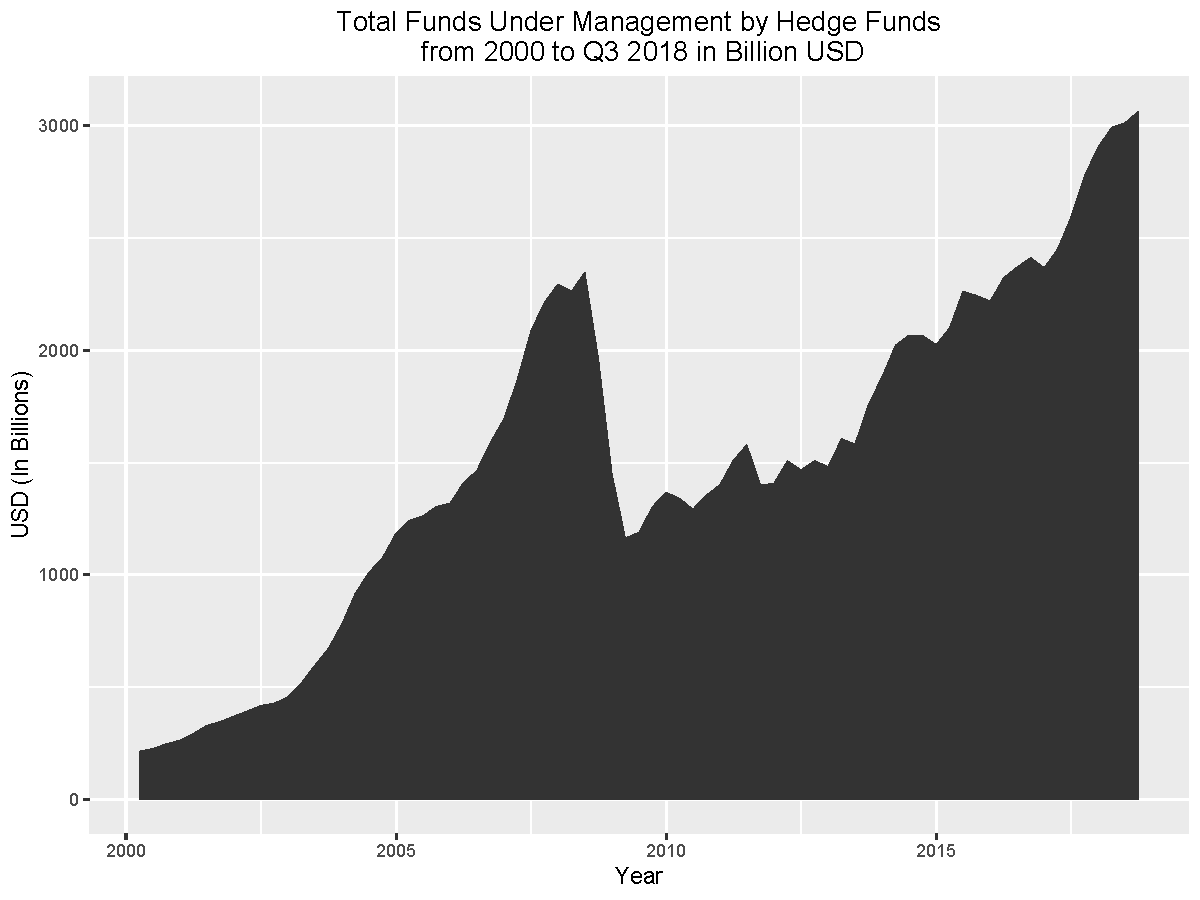
\includegraphics[width=1\textwidth]{Figures/ChapterII/Hedge_Funds_Under_Management_Barkley_Hedge.pdf}
	\caption[Funds Under Management for Hedge Funds from 2000 to Q3 2018]{Total funds under management as measured by the research firm BarkleyHedge in December 2018.}
	\label{fig:hedgefundsundermanagementbarkleyhedge}
\end{figure}
		

\nocite{BarclayHedge2018}
	

	
\subsection{Fears and Questions about Institutional Investment in the 1960s}
	
While the definition of investor capitalist can become quite broad -- anybody who engages in market activity for profit can be defined as a capitalist -- most people and institutions of modest means have a marginal impact on the market as a whole. At the other extreme, many fear that the concentration of substantial pools of capital can have a distorting effect on markets in a manner akin to how stellar objects gain influence over their peers via gravity as they accrue mass. To continue with the Newtonian gravity analogy, it was hoped that periodic disclosure of investments by the largest investors would shine a light on their stock movements and thus level the playing field with investors of more modest means. This periodic reporting would chart the distortions caused by large pools of capital, just like how gravitational distortions on other planets were used to predict and find the orbit of the planet Neptune. 
	
The legal mechanism that mandates the periodic disclosure of institutional capital is Section 13F of the SEA of 1934.  This section of law was signed by President Gerald Ford in January of 1975 and took effect in 1978 \footnote{US Code, Title 15, Chapter 2b, 78m}\nocite{US Code}. Yet, the passing of this bill was a long and tortuous affair spread over the better part of a decade and spanned four different congresses as well as the presidencies of Lyndon Banes Johnson and Richard Milhous Nixon. A look at the bill's legislative history, the rational, as well as what was discarded during the sausage-making process of getting legislation passed, can provide insight on what the bill was meant to cover, what it wasn't meant to cover, in addition to the intended use of the tools created by the bill.  
	
During much of the 1960s, there was fear that some shadowy cabal of investors were manipulating the stock market - seen as a key driver of American success in the Cold War - to their own ends and to the public's expense via underhanded techniques such as front-running and manipulating who could serve on the board of directors.  In order to allay fears and find remedies if such action were warranted, the 91\textsuperscript{st} Congress (January 3, 1969 to January 3, 1971) commissioned a study which was completed and presented in front of the 92\textsuperscript{nd} Congress \citep{Hearing71}.
	
While the 1971 report could not prove extant manipulation by institutional investors, the report did suggest that a periodic disclosure of investment positions would help allay fears by increasing transparency in the market and thus reduce the perception of corruption. Furthermore, the report shows that investors -- across different lines of investment, be it insurance, banks, pension funds among others -- were increasingly conscious of ``performance" and thus were willing to increase the risk of their portfolio in exchange for higher yields \citep{U.S.SecuritiesandExchangeCommission1971}.  However, the commission found in interviews with investors that they were unaware of the nature of the risk they were running by chasing higher yields. In order to protect investors, the report suggests that periodic disclosure of investment risk would help investors balance risk and reward in their investment decisions and looked for regulatory tools to make this a reality. The report also found that the SEC had the pre-exiting statutory authority to require increased risk reporting for mutual funds under the Investment Company Act of 1940, but that institutional investors were not covered by this Act since by their very nature institutional investors were not a public facing investment provider.  As a consequence, the SEC asked the Congress for tools to mandate regular disclosure of stock holdings for institutional investors.  
\nomenclature{SEC}{Securities and Exchange Commission}
One more problem uncovered by the report was the disparate treatment of domestic and offshore investment funds.  It was found that in practice, funds that operated outside of the territorial jurisdiction of the United States had a competitive advantage since they operated under a more permissive regulatory and taxation regime.  The report suggests that by equalizing the playing-field by forcing foreigners to register with the Securities and Exchange Commission, foreign investors would also receive stronger consumer protections.  
	
Senator Harrison Williams\footnote{Ironically Senator Williams is the only Senator successfully convicted during the ``ABSCAM'' investigation into Congressional corruption in the early 1980s. \cite{gershmanabscam1982}}  (D-NJ) shepherded the 13F amendment through multiple reform minded Congresses \citep{Shaw1981}. 	The first pieces of legislation that can be recognized as the ancestors of the current Section 13F are a pair of bills called Senate Bill 2234 and Senate Bill 2683.   The more ambitious bill (Senate Bill 2234) had a more inclusive definition of who is an institutional investor, a reporting threshold of 10 million dollars rather than 100 million dollars in S.2683, as well as mandating reporting of a broader basket of holdings, such as real estate, art, bonds, cash deposits, and commodities in addition to securities. By contrast, Senate Bill 2683 is the more modest of the two bills that Senator Williams presented concurrently to the Senate Banking committee and is substantially similar to the present section 13F of the Securities and Exchanges Act of 1934 \citep{Hearing71}. 
	
Senate Bill 2234 was deemed to be too invasive and impractical by the ranking member Bill Bennett (R-UT) since the broader basket of disclosure wasn't as easily priced as securities that are openly and regularly traded on various exchanges.  As a compromise, language was added to Senate Bill 2683 to give the SEC discretion to ratchet down the reporting threshold to 10 million dollar should they feel it necessary \citep{Hearing71}. 
	
Senate Bill 2683 sailed out of the banking committee and passed in the Senate with little opposition.  However, the bill did not make it to the House of Representatives.  Journalists covering this story attribute the failure in the lower house to the intrepid lobbying by Wall Street agents upset by the lowering of brokerage rates that was recommended by the Congressional report \citep{Zimmerman1971}.  During the lame duck session between the 93\textsuperscript{rd} and  94\textsuperscript{th} Congresses, Senator Harrison Williams went on a publicity tour in order to drum up support for the bill in the face of the New York based opposition \citep{Dallos74,Dallos74a}.  His efforts were rewarded when the language to create section 13F of the SEA of 1934 was passed by Congress early in the 94{th} Congress and was signed into law by President Gerald Ford on June 4\textsuperscript{th}, 1975 \citep{libraryofcongress}. 
	
\section{Political Regimes}	

Spatial patterns in Human Geography, and Economic Geography in particular can often show different spatial patterns from similar economic conditions due to the political and regulatory realities on the ground.  For example, \cite{Lefebvre2014} discovered that Toronto was more central to the Canadian institutional investor city hierarchy than New York City was for America.  \cite{calomiris2013} ascribes this difference to the constitutional differences in Canadian and American federalism, where the Canadian Constitution under article 91 gives the regulatory responsibility of banking to the federal government in Ottawa, whereas in the American case, the absence of explicit language dealing with banking activities in the American Constitution moved the responsibility for banking to the States under the reserve clause in the 10th amendment. 
This State responsibility for banking activities severely constrained inter-state and even inter-county business activities. 

\begin{quote}

The only real constraint was geography. Banks were not able to cross state lines and, in many states such as New York, were not able to cross city and county lines. As a result, the most successful of them were concentrated in New York City and, to lesser extent in Chicago. Their power derived from the connections they had forged over the years with businesses and corporations.\citep[p.120]{geisst1997wall}
\end{quote}

This doctrine of State banking started being reversed under the Ronald Reagan administration in response to increasing foreign competition as well as dealing with bankruptcies.  In 1982, an amendment to the Bank Holding Company Act of 1956 gave a mechanism to the Federal government to facilitate banks to buy distressed competitors across state lines as an alternative instead of relying on Federal Deposit Insurance Corporation (FDIC) funds \citep{Calomiris2000,CalomirisHaber14}.  Lastly, the Riegle-Neal Interstate Banking and Branching Efficiency Act of 1994 streamlined the process of mergers and acquisitions for financial institutions and paved the way for branch banking in the United States.

It is apparent that constitutional regimes can play a part in setting different organizational structures.  Due to the branch banking approach in the Canadian system, there are only 86 banks that fall under the supervision of the Canadian Deposit Insurance Cooperation, whereas the American FDIC insures 5 116 banking institutions \citep{CanadianDepositInsuranceCooperation2020,FDIC2020}.  This is much larger than the usual order of magnitude rule-of-thumb when comparing Canadian and American count data, indicating that political regimes can have a large influence on spatial patterns. 
	
\section{Why Geography and not Economics}


One the first papers to seriously examine the portfolio of a state pension fund is \cite{bottspension1987}.  The paper examined the investment locations for the Wisconsin State pension fund, and found that contrary to their public goal of using pension funds for the economic development of Wisconsin, a larger proportion of their investments were done in rapidly growing sunbelt states, due to their higher rate of return.  This posed an interesting question as to the priorities of State pension funds - absolute return for the beneficiaries, or should the community also benefit from this investment capital? 




\subsection{Trading in Aspatial Random Walks}
	
\nocite{Bachelier1900} 
In 1900, French mathematician Louis Bachellier submitted his thesis called \textit{"Th\'{e}orie de Sp\'{e}culation"}, in which Bachellier formulated that the long-run expected value of speculation on a market experiencing a random walk process was zero. In other words, if one were to assume that the stock market was truly random and thus had a long term trend of zero, it would be impossible to gain money off the stock market by buying and selling stocks only at the opportune time over a sufficiently long time period. While the mathematical proofs in Bachellier's work was more intuitive than rigorous, often hinting mathematical concepts that would shape the field of Mathematics in the twentieth century such as Brownian motion and Markov chains, this work was an important stepping stone to Eugene Fama's Efficient Market Hypothesis \citep{Courtault2000}. 
	
\nomenclature{EMH}{Efficient Market Hypothesis}
The Efficient Market Hypothesis (EMH) \citep{Fama1970,Fama1991} posits that asset prices fully reflect all available information.  As such, it follows that it's impossible for the average investor to continuously outperform the market average performance on a risk adjusted basis since any information is updated and baked-into the price of the security. Eugene Fama offers the theory in three related variants: Weak, Semi-Strong, and Strong. The Weak variant posits that it is impossible to derive future prices from past information, the Semi-Strong variant posits that current prices reflect all known public information and the Strong version that all information (private and public) is reflected in the price \citep{Fama1970}.  \cite{Graves2003} argues that this seminal paper cast a long shadow on the field of investment research, to the point that many papers fail to consider geography as a plausible explanation for sustained trading advantage, since it would violate the Semi-Strong and Strong version of the EMH. For example, \cite{Easley2011} find that hedge funds survive on information asymmetry, private knowledge and price ambiguity, but fail to inquire about possible sources for these sustained advantages.  Similarly, \cite{Cohen2008} find that mutual funds overweight stocks of firms in which the directors of the mutual funds have a board of directors connection with a shared educational network (\textit{alma matter}), but fail to consider current social networks and geographical proximity as confounding variables.	
That being said, the literature is rife with studies that appear to conciliate on the point that there is some geographic bias in investment returns and that these abnormal returns stem mostly from local information asymmetry. However, it does appear that this phenomenon was stronger prior to the information technology and telecommunications revolution that was ushered in during the 1980s.  
	
\subsection{Big Role for Geography} 
	
From the first market towns to Marshallian industrial districts, commerce and other economic activities are the \textit{sine qua non} of its existence. An inherent advantage of being located at a trade nexus is the ability to easily compile information on market conditions. \cite{Westaway1974} finds that as firms grow, management functions aggregate towards larger urban centres since these places have greater access to necessary specialized information.  This serves as a foundation for \cite{pred1977}, where they theorizes that the location of information-intensive activities is a positive feedback process. Furthermore, \cite{JAMES1988} as well as \cite{WheelerMitchelson89,Wheeler1989} show that urban centres see benefits proportional to their relative importance in corporate decision making.  This fits nicely with Quaternary Location Theory (QLT)\citep{Semple85}\nomenclature{QLT}{Quaternary Location Theory} which emphasises that command and control functions will naturally aggregate to large urban centres.
	
While the initial flurry of Quaternary Location Theory papers focused mostly on corporate locational preferences -- specifically command and control centres, it wasn't long before the field turned its attention towards banking and investment. An early paper \citep{greena1993} looked at the geography of institutional investment.  This paper looks at inter-city ownership of American institutional investors by using a sample of 395 institutional investors that held stocks in Fortune 500 companies for the year 1980.  In this sample, New York City is the only city in the first tier of urban hierarchy, followed by a set of four second tier cities and a steep decline thereafter.  The ranking in between city population and financial ownership is not correlated and the ordinary least-squares (OLS) spatial gravity model explains about 6 to 9 percent of the local bias in holdings.  In a follow-up paper \citep{Green1995} the author adds an additional time window (1990) and compares the new data with the data from 1980.  The OLS spatial gravity model for 1990 is quite different than the model for 1980, showing a more diffused spatial process, which the author ascribes to the increased role of telecommunications.  Green also notes the absolute increase of investors in New York City, but that its role is less dominant in the urban hierarchy in 1990 than it was in 1980.  
	
\cite{GreenMeyer1996} examined the spatial distribution of mutual funds from 1940 to 1985.  They find that most mutual funds are managed out of three main cities: New York, Boston and Chicago (in that order).  Using log-linear analysis on three explanatory variables (location  tier \footnote{Core, Semi-Core and Periphery}, year and mutual fund type), the researchers find that they can rule out a 3 way interaction, but can't rule out a 2-way interaction in the data.  Closer examination shows that the most profitable funds are located in core cities.  
	
\cite{gravesthe1998} examines the location of mutual fund companies for the year 1996. The author posits that the size of a fund is a function of the fund's past performance, and that the past performance is somewhat dependant on the amount and quality of information available. 
	
\cite{gravesthe1998} gives three reasons why mutual funds have different spatial patterns than banks.  The first reason is that mutual funds and banks have a different history of spatially-based regulations.  More specifically, mutual funds did not experience the State banking era regulatory regime.  Secondly, unlike banks which need to interact with customers on a regular basis to perform banking functions such as check cashing and bill payment, mutual funds can conduct their business by mail and other methods of communication.  Lastly, banks and mutual funds have different economies/diseconomies of scale curves with regards to personnel and investment positions.  This is mostly due to the fact that investment positions do not scale well, as they become more illiquid with size.  
	
While \cite{gravesthe1998} hypothesizes that the control nexus of investment funds will coalesce into the cities at the top of the urban hierarchy, the opposite seems to be happening, for smaller centres are growing faster than larger cities.  A possible explanation for the drop in the growth rate of funds in New York City is that modern telecommunications have reduced benefit of co-location to the point that the higher rent is no longer commensurate with the locational advantage. According to Graves, this result calls into question the ability of Quaternary Location Theory to explain the contemporary pattern of investment locations. Graves offers as an explanation that the theory was written during an era with highly aggregated data and inferior communications technology -- lacking fax, internet and low cost wireless communication.     
	
Outside of Geography and located mainly in Finance and Business, there exists a parallel literature examining the influence of locational choice and investment returns. Furthermore, this literature is highly steeped in empirical examinations over fitting evidence into established geographical theories. \cite{Hau2001} finds that traders on the Frankfurt Stock Exchange who are located in Frankfurt outperform traders located outside of Frankfurt on a intra-day basis, suggesting that there is an information distance decay function.  Similarly, \cite{Dovak2005} reports that foreign traders fare worse than domestic traders at the Jakarta stock exchange, and	\cite{choedo2004} discover that foreign-born traders pay on average 21 basis points more than domestic traders when buying stocks, and received 16 basis points less than domestic traders when selling. Meanwhile, \cite{teothe2009} found that hedge funds with offices in the same country as their investments outperform hedge funds without an office in the same country as their investment. 
	
Following this trend,  \cite{Zhu2002} used data from a discount brokerage firm and found that individual investors show a propensity to invest in companies that are local to them, and that this propensity cannot be explained by fundamentals-based investment strategies.  Since these individual investors are also more likely to invest in firms that advertise heavily, the author suggests that this is a results of investors being biased by firms they find familiar.  This finding is similar to the findings of \cite{Huberman2001}, who found that owners of Regional Bell Operating Companies tend to live in areas that were served by the company.  That being said, \cite{Monk2009} states that while investing in firms in which the investor has a high level of familiarity may represent a sub-optimal strategy from the point of view of traditional portfolio theory. In some cases, it can provide for those willing to look beyond the efficient market hypothesis a source of information overlooked by the market and thus a way to profit from information asymmetry. That being said, well publicised investment flops in which State pension funds are used to prop-up failing local champions leading to large losses, such as the 80 percent haircut the State of Connecticut experienced on its loan to Colt Industries in the early 1990s, can make this type of strategy politically difficult to execute. 
	
\cite{Bradley2016} report that, in a sample of 16 internally managed state pension funds, they are over-weighted in local companies by 26 percent relative to the average portfolio.  Furthermore, these investments occur predominately in companies that are active in local politics, as measured by both political donations and active lobbying.  The authors explore three non-mutually exclusive explanations for this over-investment: 
\begin{enumerate}
	\item \textbf{Information advantages due to local effect:}  This theory posits that political connections lead to better information flow to the pension fund trustees, and this can be used for trading advantage.
	\item  \textbf{Familiarity:}  This theory posits that managers are more familiar with local firms and over-estimate the quality of their information, but is otherwise a neutral position.
	\item \textbf{Pay to Play:}  This theory posits that political bias and influence peddling leads to malinvestment of State pension funds into politically connected firms.  These conflicted motives lead to worse performance. 
\end{enumerate}
In total, the evidence (that the effect is stronger in States with a larger share of politically appointed pension fund board trustees as well as States with more powerful members of congress) points towards solution 3 as being the most likely.  
	
\cite{malloythe2005} reports that geographically proximate analysts outperform distant analysts in their buy and sell recommendations. The author posits that analysts who make house calls rather than conference calls can obtain more valuable and actionable private information via face to face communication, direct view of the operations floor, talk to floor employees as well as being better positioned to talk to suppliers.  The effect is stronger in smaller locals.  Similarly, \cite{Farooq2013} studied the buy and sell recommendations by foreign and local stock analysis covering Thailand, Indonesia, Malaysia and South Korea during the Asian Financial crisis (1997-1999).  This study found that foreign-based analysts had more accurate buy recommendations, whereas local analysts had more accurate sell recommendations.  Furthermore, \cite{Eckel2011} found, via spatial regression analysis, larger returns than what would be expected for investment firms that invested in companies within a headquarters with 50 miles of their location compared to a random portfolio of companies with similar attributes.  
	
Continuing on the theme of information decaying over distance providing real investment advantages,	\cite{Cashman2017} use the cost of borrowing capital for publicly traded real estate companies in Asia-Pacific as a proxy for the cost of information opacity. The authors conclude that more diffused firms (those operating in more than one country) have higher capital costs than firms that only operate in one country and thus they posit that companies pay an opacity tax.   

In an interesting parallel to the debate on the importance of Marshallian agglomeration with regards to footloose industries, that is to say those that do not necessitate large fixed upfront costs such as factories, \cite{Mitchell_London_2019} looks at the productivity of literary authors of the 18\textsuperscript{th} and 19\textsuperscript{th} century. This study found that when controlling for a multitude of factors authors were most productive when located in London UK and that there's a statistically robust relationship between time spent in London and increased productivity.  Furthermore, the results of this paper suggest that there was a benefit to being located in London that was not present in other UK and Irish literary cities such as Edinburgh or Dublin.  The paper posits that geographic concentration fosters thicker social networks with their peers, individuals of influence (agents, editors, publishers) and patrons, thus facilitating the ease of getting published. 	
\nomenclature{OLS}{ordinary least squares}
	
\subsection{Moderate Role for Geography}
	
There exists an other branch of the literature that walks the middle ground between the importance and irrelevance of space with regards to investing.  At a coarse level, this literature can be summarized as believing that locational advantages were quite measurable prior to the telecommunications revolution of the 1970s and 1980s, and accepts a limited role at best for locational advantages to accrue in the face of modern telecommunications technology.
	
During the time period between 1925 and 1978, \cite{rhoades1982size} looked at the distribution of deposits in commercial banks and found that due to bank consolidation that were mostly driven by mergers and acquisitions, the distribution of bank deposits were increasingly concentrated towards the top end of the top 100 largest banks list. Furthermore, while this period saw important demographic changes in the US with the increasing population in the Southern and South-Western United States, changes in the location of the top 100 largest banks were less reflective of the demographic shift than would be expected in a naive model in which bank size is a function of population.  This suggests that large urban centres with preexisting banking infrastructure have an innate pull factor that make banks less footloose than would otherwise be assumed.  
	
With a more expansive look at locational preferences, \cite{bodenmanthe1998} examines the exodus of  Finance, Insurance and Real Estate (FIRE)\nomenclature{FIRE}{Finance, Insurance and Real Estate} sector firms in downtown Philadelphia, Pennsylvania.   During the period between 1983 and 1993, the concentration of FIRE firms located in downtown Central Business District (CBD)\nomenclature{CBD}{Central Business District} fell from 61.9 percent to 24.9 percent.  Examining why firms were leaving the Central Business District, the author asked FIRE sector businesses for factors that were at the heart of the locational preferences.  Personal preference and quality of life were given as top answers, whereas access to information was not given as a priority.  In a related study, \cite{bodenmanfirm2000} looks at how the information technology revolution permits institutional investors broader choice of location without sacrificing access to high quality and quantity of data/information.  Bodenman finds that not all actions taken by institutional investors require face to face contact, such as accounting and regulatory compliance, portfolio management, and trading.  In contrast, activities that do require face to face contact, such as finding and/or managing clients as well as researching investment opportunities do not require a constant downtown presence. As a consequence, \cite{bodenmanfirm2000} posits that active traders will have a propensity to locate in the CBD, whereas passive investors and quantitative traders will locate in suburban office parks where rent is less expensive.  
	
\cite{gongthe2012} examine the geographical dispersion and return on the island of Manhattan shortly before and in the aftermath of the 9/11 terrorist attack. Of the 79 firms surveyed, fifty-four did not change location, while ten moved on a temporary basis (one month to a year and a half), and fifteen changed locations permanently.  Of the ten who changed locations toward the periphery of the New York area, the most common reason for returning to Manhattan is the ability to meet with clients.  Most of the firms that moved were located in Downtown and Midtown, in contrast,  those that returned were located exclusively in Downtown Manhattan. Furthermore, the survey says that prior to the 9/11 attack, most firm managers were reporting that their locational preferences were shaped by maximising the prestige of the building, adjacency to the New York Subway system, as well as being conveniently located in order to meet with clients.    After the attack, the location preference was dominated by an emphasis on office space, building infrastructure and rental costs, while keeping in mind that high prestige buildings would be more susceptible to terrorism in the future.  
	
\section{Conclusion}	

The literature on location choice for stock market investors can be divided into three broad categories.  The first stems from the Eugene Fama's Efficient Market Hypothesis  and Louis Bachellier's  \textit{``Th\'{e}orie de Sp\'{e}culation"}, which states that it should be impossible to derive a long term trading advantage from one's physical location.  The second stems from a more Industrial Geography perspective that values the use of tacit knowledge networks derived from co-location to create long-term trading advantages \citep{Westaway1974,covalthe2001}.  The last category tries to bridge the first two, for the telecommunications revolution has reduced the benefits of co-location and thus liberalized location choice as explored by \cite{Moriset2009} where they argue that modern telecommunications re-arrange spatial forces of agglomeration, and thus reduces the need for vertical hierarchies.  The following chapters will examine which school of thought on location choice best reflects the actual location of investment firms in the twenty-first century.

%While we may not have seen the death of distance as predicted by \cite{Obrian1992}, \cite{gongthe2012} described the stickiness of location choice in Manhattan, despite it being one of the most expensive real-estate markets in the world, explicitly showing that co-location is important factor in location choice.  That being said, it can be argued that while there is a role for space and place, the telecommunications revolution may reducing the benefits of co-location. This is the main trust of the paper by \cite{Moriset2009} where they argue that modern telecommunications re-arrange spatial forces of agglomeration.  Better communications reduces the need for vertical hierarchies and remove the premiums of co-location, and by extension allows for the liberalization of location choice. 


	
	
	
	

		\chapter{The Data Pipeline}
\label{ChapterIII}
\nocite{rgdal}
\section{Introduction}


The 13F-HR report is the cornerstone of this study, for it offers a very detailed peek into the stock holdings of all institutional investors with holdings above 100 million dollars USD in fair market value, as well as voluntary reports for firms with smaller holdings\footnote{Some institutional investors with holdings under 100 million USD are compulsory rather than voluntary in nature due to having exceeded the 100 million USD reporting threshold in the previous 4 quarters.}.  Understanding the data pipeline, that is to say how the data went from the SEC's Edgar server, wrangled into the databases, and then cleaned prior to use in statistical models is important in understanding the strengths and limitations of these models.  Otherwise it's garbage in, garbage out (GIGO) research.  

\section{The 13F-Holding Report}

There are countless news articles that use 13F-Holding Reports (13F-HR) data as a basis for ``whale watching", that is to say, poring over the 13F reports of successful investors such as, but not limited to Warren Buffet, and imitating their strategies and/or replicating their holdings on a smaller scale \citep{Whale_Watching_CNBC_12}.  While some may debate the wisdom of buying and selling stocks based on what experts were holding 45 days in the past\footnote{13F-HR reports are due to the SEC for public access no more than 45 days after the end of a quarter.  For example, reports for the period ending March 31st would be due no later than May 15th (or the next Monday if that date would fall on a Saturday or Sunday)}, other say that these reports allow smaller investors to gain insights based on the research departments of larger investors \citep{WhaleReport13}.  

The data for this thesis was collected from the SEC's Edgar database between 2015 and February \nth{18}, 2019.  The Edgar database provides 13F filings in two different formats.  The first of these formats is the ``.txt" format, which covers the period of March 31, 1999 to March 31, 2013. It should be noted that despite the existence of older filings on the Edgar server prior to March 31, 1999, these filings covering the time period of 1990 to 1998 only exist for a handful of filers each quarter and thus would provide an incomplete and biased sample.  This era of filings contain holding information in an unstructured format that are easily human readable, but unreliable when parsed by computers.  The second era of filing formats covers the periods of June \nth{30}, 2013 to December \nth{31}, 2018.  These filings are in the newer ``XBRL" file format which is a derivative of the popular ``XML" file structure.  This file format has the benefit of being easily machine readable.  Furthermore, all 13F-HR/A files represent amendments to previous filings were integrated in to the database. 

Due to the difficulties in parsing the older ``.txt" file formats, this mandated the creation of two different databases of institutional investors.  One piece of information that was easily extracted from the ``.txt" files was the business address of the investor.  This leads to the creation of a database containing what is essentially a ``phone book" information for all institutional investors that filed at least one quarterly report during the 20 year period covered by this research ($n = 242084$). The second database is derived from the ``XBRL" encoded files and contains a list of all positions reported by the filer to the SEC. Since some filers chose to disclose more information than required, and in the interest of maintaining a fair comparison across firms, only positions containing securities were kept in the database ($n=92539$).  

\label{Section:13F}

When plotting the duration of how long different filers (as defined by unique Central Index Key (CIK)) exist in the database, as seen in Figure \ref{fig:countoffilers}, one notices a pattern in the data where peeks can be found at $n+1$ quarters where $n$ is zero or an integer divisible by 4.  The most likely explanation for this reporting artifact is the requirement to report for the next four quarters after which they have fallen back under the 100 million dollar reporting threshold.   

\begin{figure}
	\centering
	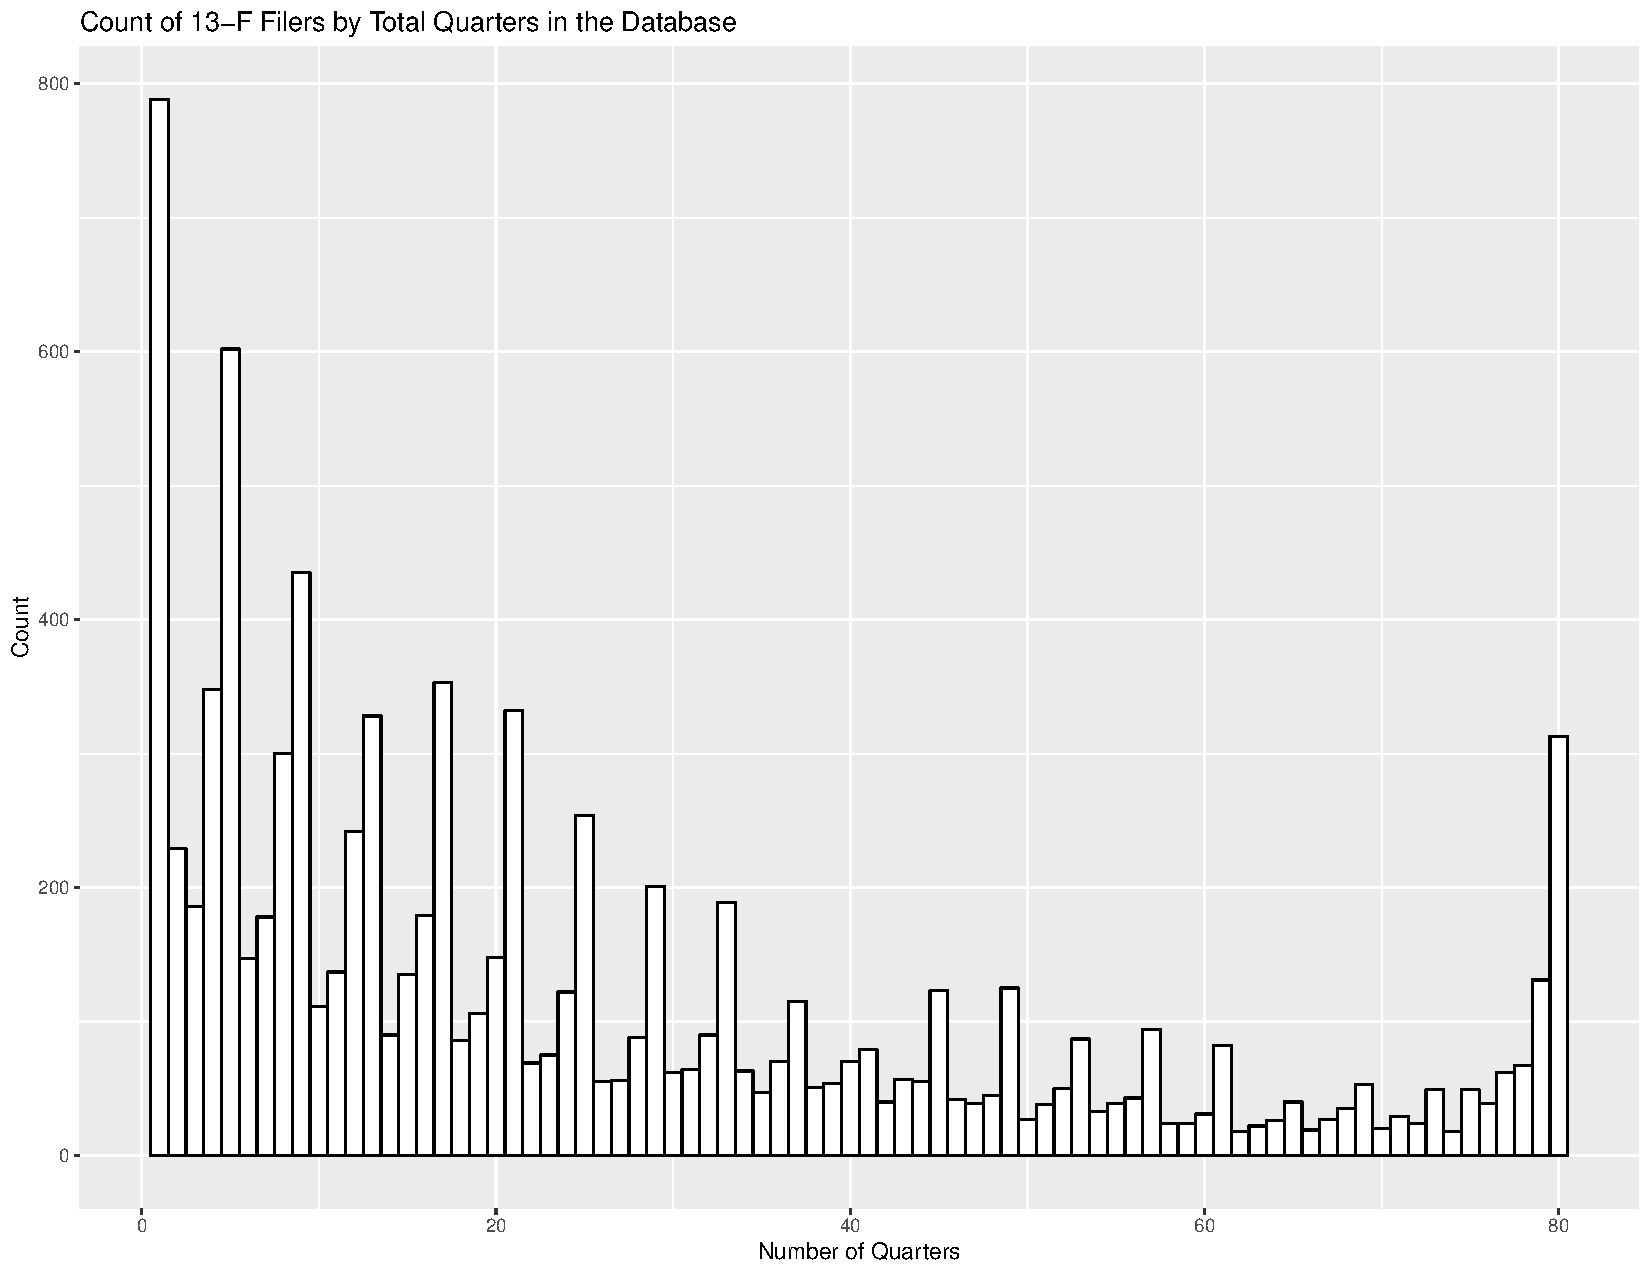
\includegraphics[width=1\linewidth]{Figures/ChapterIII/Count_of_Filers}
	\caption[Count of 13-F Filers by Quarter]{Count of 13-F filers by quarter in the EDGAR 13-F Database. One should note the regular pattern of $n+1$ quarters, where $n$ is zero or an integer divisible by 4.}
	\label{fig:countoffilers}
\end{figure}



\subsection{Investors by Country}


While these filings are filed under pain of perjury, there is no guarantee that these filings are a true and accurate reflection of the investor's books\footnote{For example, Bernie Madoff's fraudulent fund is still listed in the pre-2008 data}.  In fact, the SEC's EDGAR server warns users that they are not responsible for any damages caused by acting on incorrect information.  In line with this warning, it is obvious that some filings are incorrect.  In a few cases, one quarter's filings were orders of magnitude larger than all other filings reported by that filer.  For example, Firm 0000863748's filing for March \nth{31}, 2016 reported a total fund value of 5,632,710,967,874.14 USD.  This value is more than twice the value recorded for BlackRock family of funds, as well as being orders magnitude larger than the neighbouring filings.  While there is no absolute guarantee that all filings are accurate, the yearly totals were verified for anomalous values using the Rosner Test as found in the EnvStats R package \citep{EnvStats-book}. During the period of June 2013 to December 2018, there were 570 filings with anomalous top-line values flagged by the Rosner Test. However, not all abrupt changes in top-line valuation are due to erroneous filings.  One such example is BlackRock which underwent a change of reporting scheme for 2017 onwards, where it decided to consolidate more reports under one filing ( BlackRock Advisors, LLC, BlackRock Fund Advisors, BlackRock Investment Management, LLC, BlackRock Group Limited, BlackRock Institutional Trust Company, N.A. and BlackRock Japan Co., Ltd.), and thus went from reporting 70.6 billion USD to 1.8 trillion USD. For the suspect filings that could not otherwise be explained, these values were extracted from the database and replaced with a synthetic entry using a weighted average of the surrounding 4 quarters\footnote{The main weighting is a (0.2/0.3/suspect entry/0.3/0.2), however, June 2013 and first company filings are treated with a suspect entry/0.6/0.4 (opposite weights for last filing and December 2018), the filing for September 2013 and filers with suspect second entry is 0.4/suspect entry/0.4/0.2. (Inverse weights for September 2018 and December 2018)}. 

This is further complicated by the fact that the legal basis for 13F-HR disclosure mandates only the disclosure of securities and thus the conversion of an investment position to a non-reportable position has a warping effect on the top-line value for each fund. For example, if an investor were to convert a million dollar position in a company into a million dollars worth of real estate, the 13F-HR filing would show a drop of 1 million dollars in the subsequent filing, however the fund's true bottom line did not change.  Furthermore, research conducted by \cite{griffinhow2009} looked at the difference between institutional investors and mutual funds, and how they organize their respective short and long positions.  As a matter of law, mutual funds can't short stocks and thus are forced to make their profit off of their long positions.  By contrast, the hedge fund's more permissive regulatory regime allows for short-selling and thus allows for the set-up of using long positions for hedges, and short-selling as a profit-generator.  That being said, the researchers found that there is no statistical difference between the long position profitability between hedge funds and mutual funds.  As a consequence, the long positions as reported in the 13F-HR filings should still hold valuable insights in corporate command and control functions, especially since many firms have a waiting period before the power to vote on board of directors vest.  



\nomenclature{USD}{United States Dollar}

Interestingly, Bernard L. Madoff Investment Securities LLC (CIK number 00001386924) exists within the database from June 2006 to September 2008.  However, as was revealed in December 2008, Bernie Madoff was at the centre of a 50 billion USD Ponzi scheme \citep{Appelbaum2008} in which instead of investing his client's money, he would deposit investments into his personal bank account, as well as pay redemption from this account.   As Harry Markopolos detailed in his testimony to the House Financial Services Committee in the aftermath of the Bernie Madoff scheme's unravelling, use of 13F-HR should have uncovered the scheme years earlier, since what he reported on the disclosure form did not match what he was telling clients \citep{Marko09}.   Due to being a known fraud,  Bernard L. Madoff Investment Securities LLC (CIK number 00001386924) was censored from the database.  While it's unknown how many other fraudulent investment funds exist, there is no other choice than to believe that all the filings are done in good faith, and that the 570 anomalous filings were based on human error.  

\section{Tying Capital to Physical Space}

Financial Capital is inherently global while money often acts on the local scale \citep{clarkmoney2005}.  An apt metaphor according to Clark is that money will flow like mercury due to the following properties: 


\begin{quote}Characteristically, mercury tends to (1) run together at speed, (2) form in pools, (3) re-form in pools if disturbed, (4) follow the rivulets and channels of any surface however smooth it may appear to be, and (5) is poisonous in small and large doses if poorly managed. \citep[p105]{clarkmoney2005}
\end{quote}

These characteristics can make mapping global finance difficult. With the information available in the form 13F-HR, the best one can do to tie the command and control functions of the decision makers is to use the business address in which investors deal with the US regulatory system, and the Securities and Exchange Commission in particular. 


\section{The Time Period}
\begin{figure}[H]
	\centering
	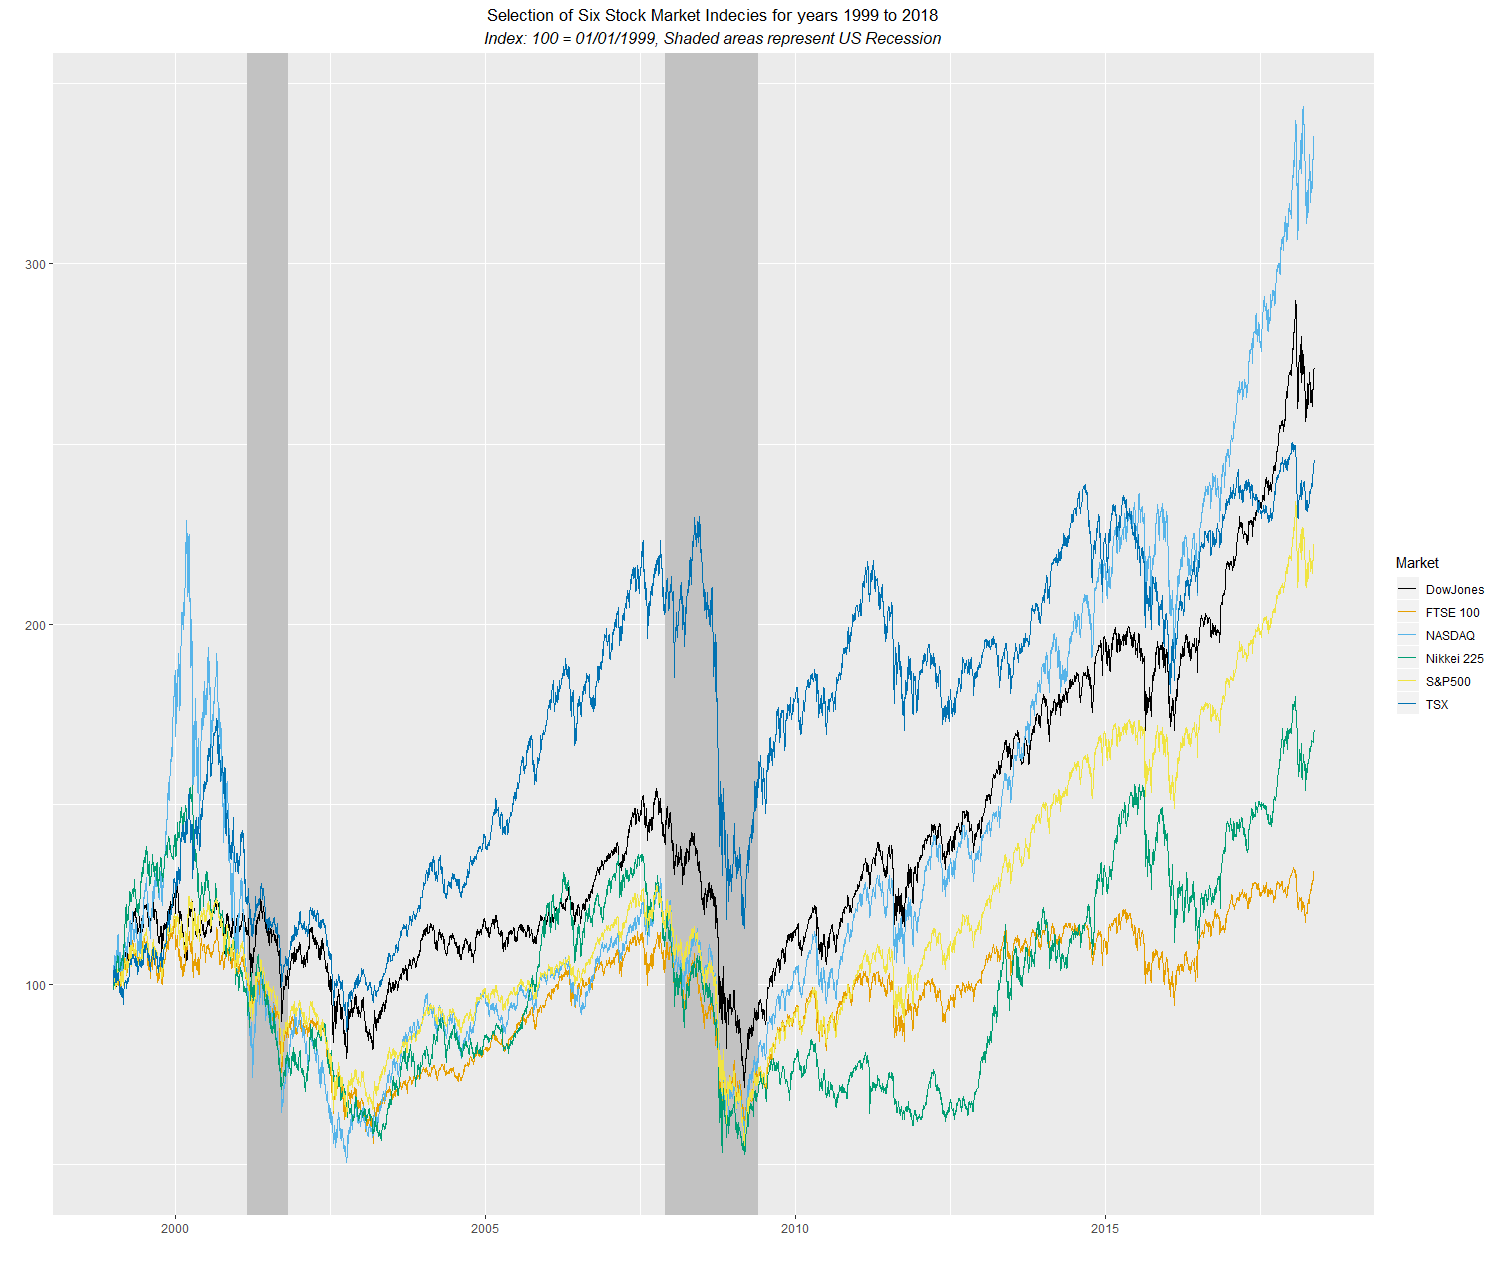
\includegraphics[width=1\textwidth]{Figures/ChapterII/Stock_Market}
	\caption[Stock Indices for 1999 to May 2018]{Collection of six stock indices for the years 1999 to 2018. The information was collected from Yahoo! Finance API on December 28, 2018.  Shaded Areas represent recessions as defined by the National Bureau of Economic Research's Business Cycle Dating Committee \url{https://www.nber.org/cycles/cyclesmain.html}.  The first recession dates from March 2001 to November 2001 and the second dates from December 2007 to June 2009. }
	\label{fig:stockmarket}
\end{figure}

Stock market indices provide a general guideline on the overall health of the stock market \citep{Lo21}.  From the investor's point of view, this is often used as a performance benchmark in which to evaluate their return \textit{vis-a-vis} their peers. Figure \ref{fig:stockmarket} shows a collection of six stock indices.  Three of these indices are used as bell-weathers of the US Stock-Market: The Dow Jones Industrial Average (DJIA/DOW)\footnote{The Dow Jones Industrial Average is an index of 30 blue chip US stocks covering the US economy except for transportation and utilities.  The mix of 30 stocks has changed over time to reflect changes in the economy \citep{DOW2020}.}, The Standard and Poors 500 (S\&P 500)\footnote{The S\&P 500 is an index of 500 large-cap stocks that tries to be representative of the US economy \citep{SNP2020}} and the National Association of Securities Dealers Automated Quotations Composite (NASDAQ Composite)\footnote{The NASDAQ is a broad-based index of over 3000 stocks listed on the NASDAQ stock exchange.  This index is heavily weighted towards the tech sector, and as such the ``irrational exuberance" of the DotCom era cast a large shadow over this index, taking 15 years to surpass to the record highs that were recorded during this era (NASDAQ, 2018)\nocite{NASDAQ2018}.}.   The three other indices give insights to the national stock markets of various important regions for this study.  The first is the UK's FTSE 100, Japan's Nikkei 225 and Canada's TSX.  

Examining the correlations over time of various stock index is beyond the scope of this thesis, one would be remiss to forget to draw attention to the correlated nature of the various stock indices.  That being said, being aware of the general nature of the stock market (Bear vs Bull market) gives context to whether growth in an investor's position can be partially explained by capital gains rather than attracting new clients and capital.  More specifically, the 20 year period of 1999 to 2018 is an era that can be characterised as having strong overall growth, punctuated by two rather large financial crises: the DotCom crash of 2000 and the Great Financial Crisis of 2008-2009.  As a consequence, this time period contains 2 powerful bull markets in which the market recovers powerfully from crash.  The first being the mid-aughts economic boom and the other the Obama recovery.



\nomenclature{NASDAQ}{National Association of Securities Dealers Automated Quotations Composite}
\nomenclature{S\&P 500}{The Standard and Poors 500 Index}
\nomenclature{DJIA}{Dow Jones Industrial Average}
\nomenclature{DOW}{Dow Jones Industrial Average}

While stock markets are somewhat useful in determining the scope and duration of a recession, \cite{Samuelson1966} oft-quoted quip of ``the
stock market has forecast nine of the last five recessions" has a certain amount of truth to it. This is why the significant stock market correction that took place in 2016 isn't shaded as a recession in figure \ref{fig:stockmarket}, since this did not have a significantly negative impact on the broader economy. This is why the National Bureau of Economic Research (NBER) does not have a fixed definition of what exactly constitutes a recession, going for an approach similar to Justice Potter Stuart's definition of obscenity - ``You know it when you see it" (Jacobellis v. Ohio, 378 U.S. 184. 1964). As such, the NBER's Business Cycle Dating Committee is charged at taking a holistic view of the economy when determining the length and breath of a recession such as changes in employment, housing starts, payroll numbers, manufacturing output and aggregate hours worked in the economy rather than fixate of certain metrics such as stock market contractions or changes in Gross Domestic Product \citep{NBERBCDC2020}.  




\section{Conclusion}


This section explores the data collection pipeline from the SEC's Edgar server to the decision to create two separate databases of 13F investors. As seen from the examples of inconceivable wealth declared in certain 13F-HR files due to various clerical errors, the data cleaning was an important factor in being able to trust the outputs of the models.  Furthermore, the inability to trust the semi-structured text format led to the creation of the "phone book" database and the more machine readable ``XBRL'' based database.  The first database covers the time period of 1999 to 2018 and contains what is essentially phone book information such as years active and locations. The more detailed ``XBRL'' based database covers the time period of June 2013 to December 2018.  This second database contains a detailed stock listing of their end of quarter holdings.  Both databases were then geocoded using Google Maps API.  Next, these databases were contextualized by exploring the time period in which they were active.  

In the following chapters, these databases will permit this paper to map the evolution of institutional investing in the United States for time periods they cover in order to examine if there are any significant changes in the hierarchies of cities from the time of \cite{greena1993} and \cite{gravesthe1998}.  Secondly, the more detailed database will allow for the examination of whether portfolio preferences play a role \textit{vis-a-vis} the locational choices of investors.  


		\chapter{Exploring the Data}
\label{ChapterIIIb}
\section{Introduction}

Statistician John Tukey is a strong advocate for exploratory data analysis (EDA).  Collectively, EDA is a series of graphical and quantitative techniques used to explore novel data in order to examine its data structure, and thus generate insights that can be used as a springboard for hypothesis and model generation \citep{tukey77,Hoaglin1982}.  

This chapter performs EDA on the data at various ground scales (country, state, core-based statistical area (CBSA), county and point) using a variety of techniques such as simple counts to more elaborate techniques such as Ripley's K and the gravity model of trade. 

\nomenclature{EDA}{Exploratory Data Analysis}
\section{Count and Percentage by Region}
\begin{figure}[h]
	\centering
	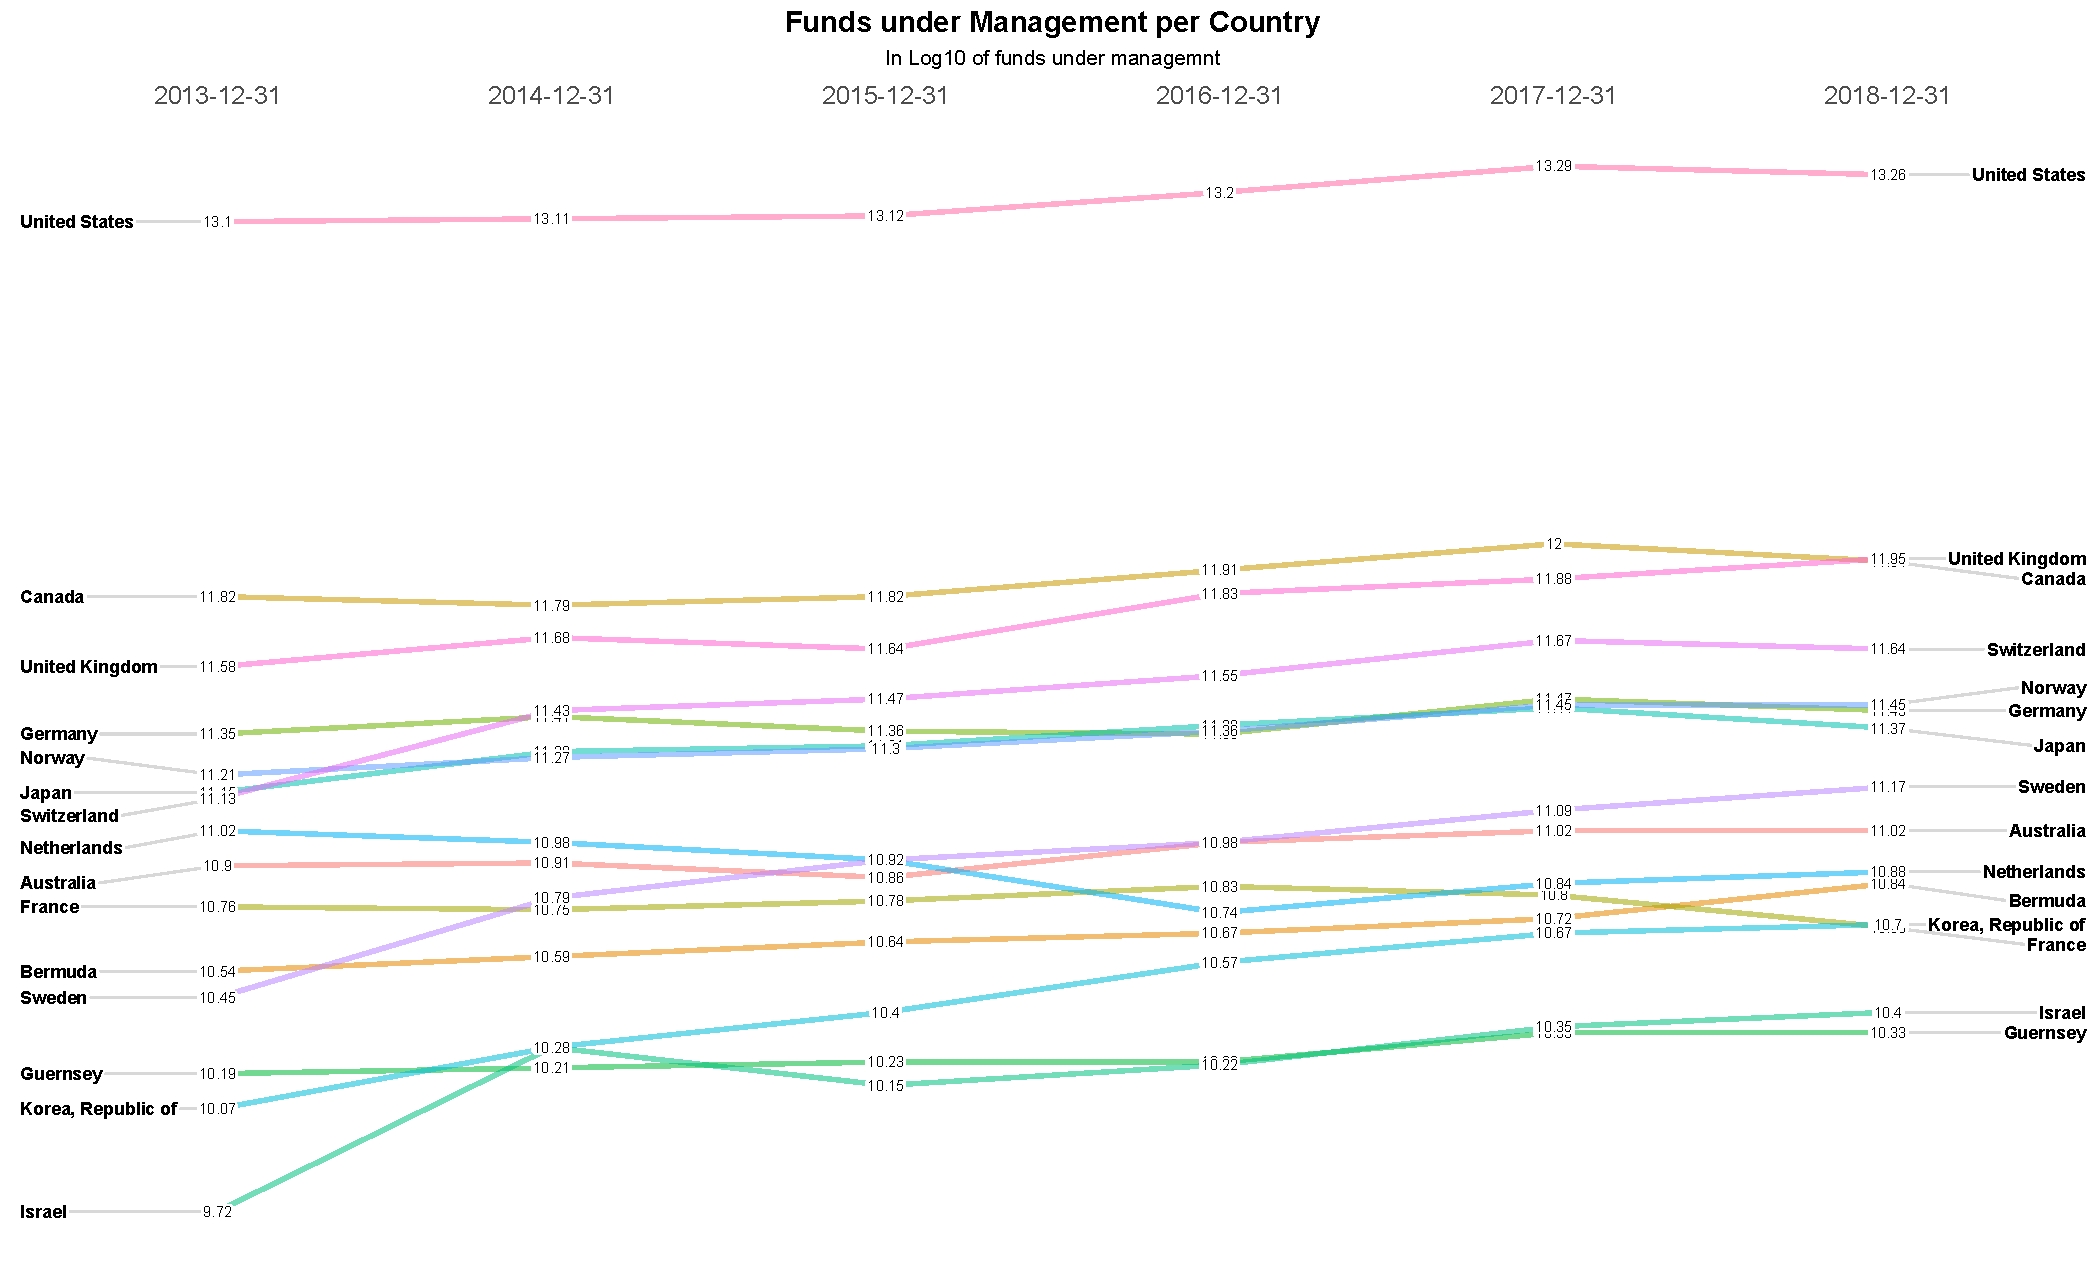
\includegraphics[width=1\linewidth]{Figures/ChapterIII/Funds_Per_Country_Slopegraph}
	\caption[Funds Under Management per Country in Log10]{Funds under management by country/political entity for top 15 countries in the world by funds under management.  Due to the very large gap between the USA and all other countries, the dollar value is represented in log10 form.}
	\label{fig:fundspercountryslopegraph}
\end{figure}


Figure \ref{fig:fundspercountryslopegraph} is a slope graph showing the sum of funds under management for all firms headquartered in each country.  As explored earlier, the 13F holdings report is a US legal instrument primarily interested in reporting the holdings of shares of US headquartered companies. It is no surprise that the United States of America is over-represented in this database.  Furthermore, since many of the other countries on this list have their own robust domestic stock markets, one should take caution before making direct comparison between the US-based investors and foreign investors.  Secondly, it is interesting to note that Canada, despite being a smaller economy than the United Kingdom, is home to more investors as measured by funds under management than UK based investors\footnote{This is strictly true provided that Crown Dependencies (Guernsey, Jersey, and the Isle of Mann) and British Overseas Territory (Gibraltar and Bermuda being the most prominent) are excluded from the UK's total.  With respect to the law, the Crown Dependencies are not part of the UK legislative and legal apparatus, and are autonomous with regard to their legal system, however the Crown is ultimately responsible for maintain good governance of these territories.  \citep{CrownDependencies}}. Finally, it is not surprising that the list of countries in Figure \ref{fig:fundspercountryslopegraph} are mostly populated by advanced economies and countries/political entities that specialise in financial services, such as Switzerland, Guernsey, and Bermuda.



\subsection{Investors By State}

While the 13F data has global reach with regards to foreign investors using US investment system, the use of domestic stock market is a significant confounding variable.  Therefore, for practical purposes, the focus of this research will be centred to a greater extent on the United States of America, its commonwealths and oversees territories.

\begin{figure}[h]
	\centering
	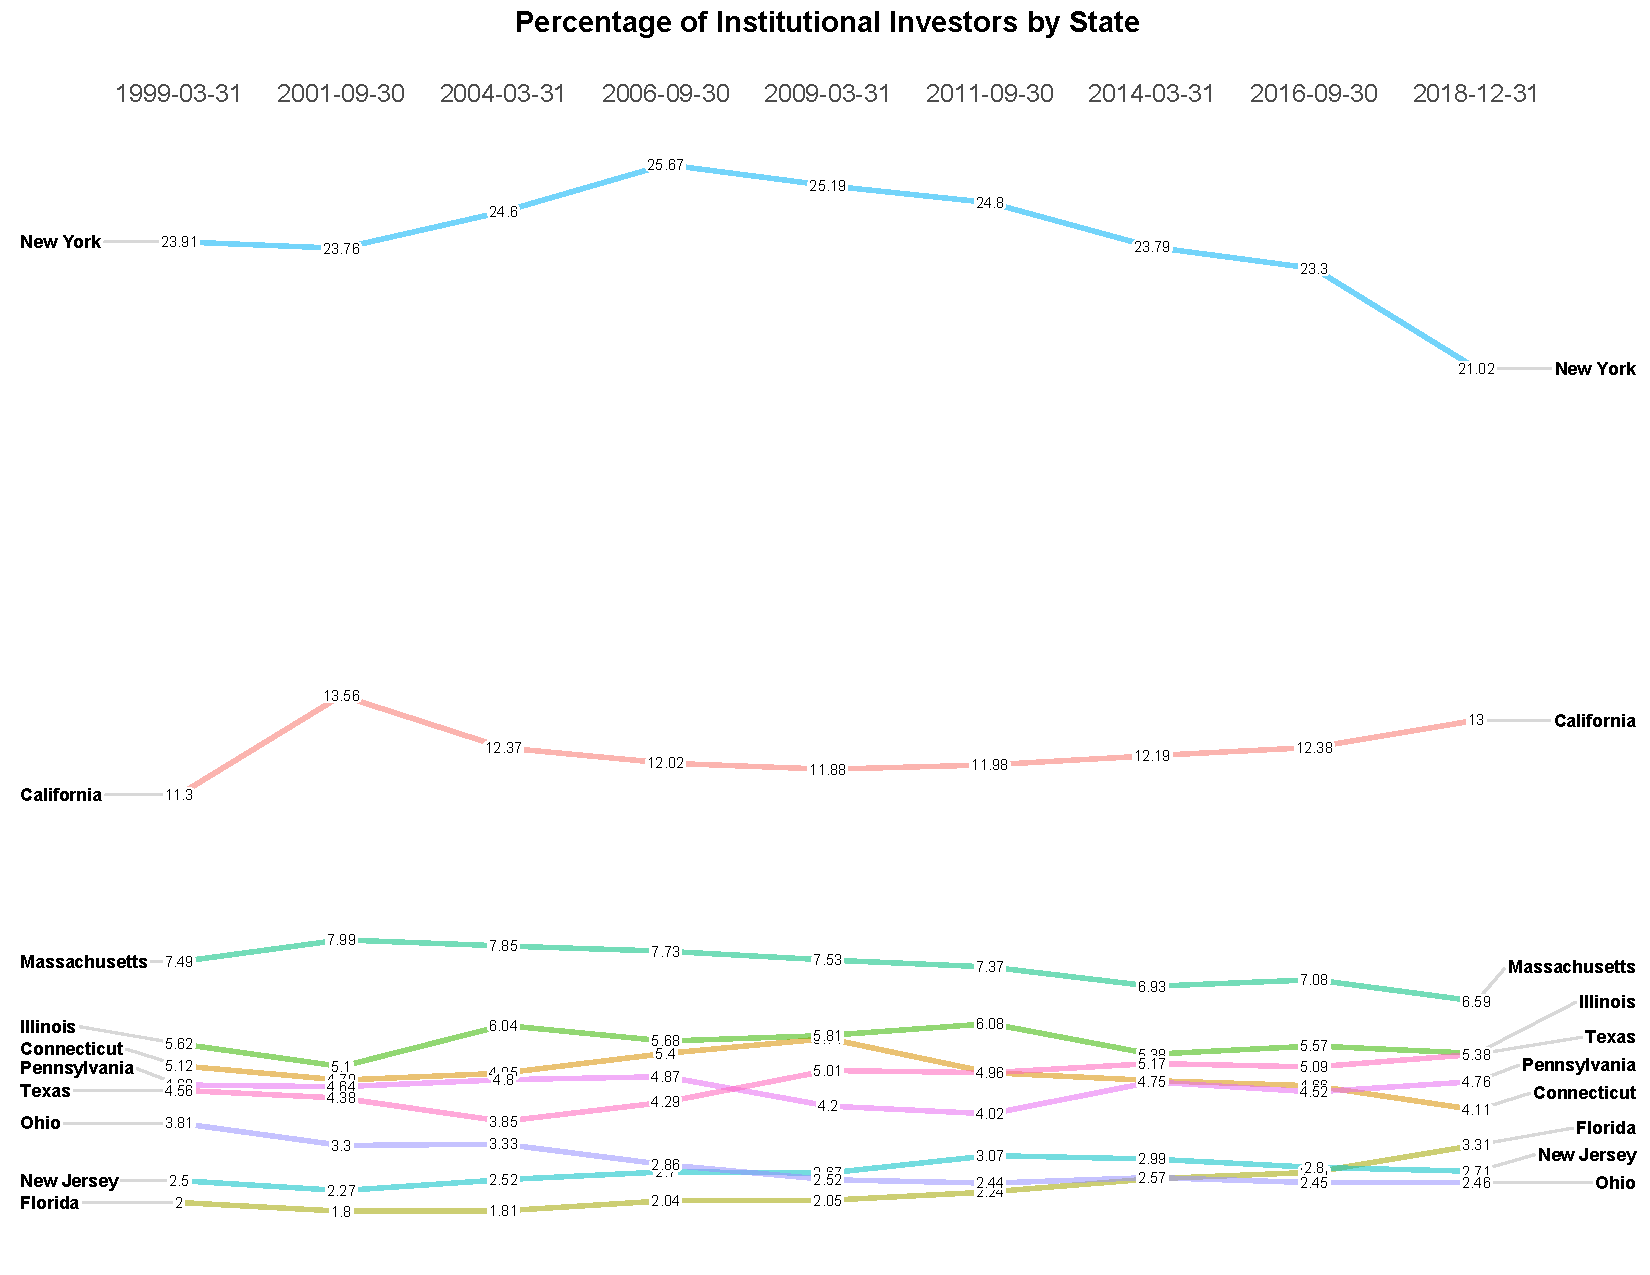
\includegraphics[width=\linewidth]{Figures/ChapterIII/Precentage_State}
	\caption[Percentage of Investor by  by State]{Percentage of Institutional Investors locational preference by share of investors by State.}
	\label{fig:precentagestate}
\end{figure}
There exists institutional investors in every US State, however there is a very unequal distribution when it comes to their location, by both number of investors and funds under management. \cite{WheelerMitchelson89,Green1995,bodenmanfirm2000, Graves2003} have seen and forecasted the continued relative decline of New York, and specifically it's namesake city.  And yet, despite the continual relative decline of New York State's position at the centre of the United States's financial system (Figure \ref{fig:precentagestate}), New York State is still home to the largest growth in institutional investors in absolute terms for this time period (Figure \ref{fig:countiibystate}). It should be noted that the renewal of New York's relative decline resumes on or around the first quarter of 2007.  This will be discussed in further detail at the county level (Section \ref{investorsbycounty}) and in point pattern analysis using Ripley's K (Section \ref{kfunction}).  	

\begin{figure}[h]
	\centering
	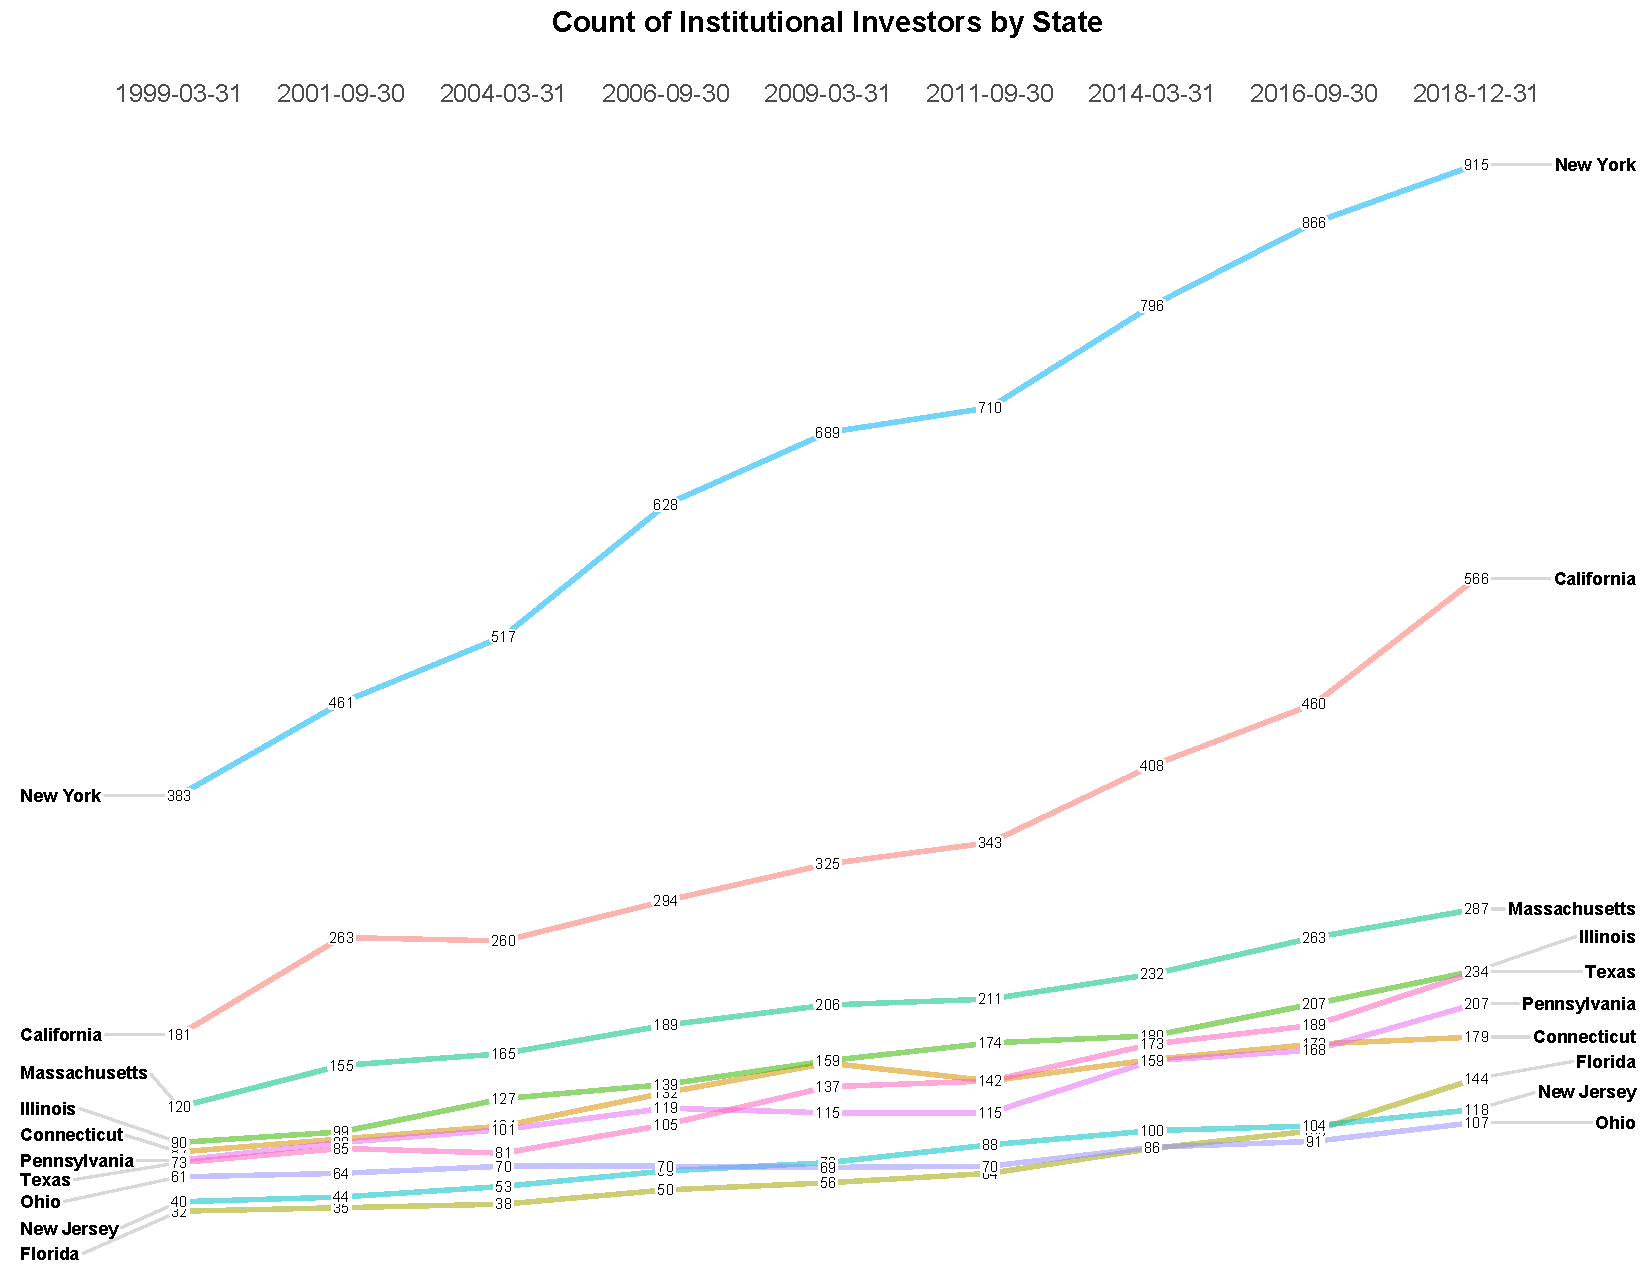
\includegraphics[width=1\linewidth]{Figures/ChapterIII/Count_II_BY_State}
	\caption[Count of Institutional Investors by State]{Count of Institutional Investors by State for the period 1999 to 2018.}
	\label{fig:countiibystate}
\end{figure}

While the region that contained the former industrial heart of the United States of America is experiencing a rather severe relative decline, these regions still manage to grow their number of firms in absolute terms.  This suggests that the cause of relative decline is a slower genesis of new firms rather than a migration of footloose firms.  This is consistent with the findings of \cite{gongthe2012}, which shows that despite large shocks, a firm's geographical preferences are sticky.  

Further evidence for the point that firms are sticky can be found in figure \ref{fig:distancemovedhistogram}, where the great circle distance was measured between the locations of the first and second, second and third, third and fourth, ect... locations of firms in the ``phonebook'' database of 13F filers created by the author.  In the database there are 14 922 unique location and CIK combinations, of which 5 603 firms (CIK) stay in the same location for the duration.  For the remainder of 3 649 firms (CIKs), the database show them making 5 190 moves, for a total of 9 319 unique CIK/locations.  While this 9 319 unique locations may make the moves to appear very footloose, one must remember that a move implies two distinct locations.  In this database, the most footloose firm has a total of 7 moves, but this is the far end of the distribution as seen in Table \ref{tab:Numberofmoves}.  

% Table created by stargazer v.5.2.2 by Marek Hlavac, Harvard University. E-mail: hlavac at fas.harvard.edu
% Date and time: Thu, Feb 20, 2020 - 2:39:04 PM
\begin{table}[!htbp] \centering 
	\begin{tabular}{@{\extracolsep{5pt}} lccccccc} 
		\\[-1.8ex]\hline 
		\hline \\[-1.8ex] 
		Number of Moves & 1 & 2 & 3 & 4 & 5 & 6 & 7 \\ 
		\hline \\[-1.8ex] 
		Count & $2,477$ & $886$ & $221$ & $52$ & $9$ & $3$ & $1$ \\ 
		\hline \\[-1.8ex] 
	\end{tabular} 
	\caption[Number Moved by Firms]{Number of Moves by an Institutional Investor between the years 1999 and 2018}
	\label{tab:Numberofmoves}
\end{table} 

During this time period, 4 917 of 5 190 (94.7\%) of location changes have been what can be considered intra-city/intra-metro area (less than 150 km) rather than 
47
 inter-city.  This lack of long-distance movement makes attracting firms to a new locale a near-non factor in location changes over time, suggesting some costs in movement, or that rent isn't a top-line deciding factor in location.  Even more important for how sticky firms are in their locational preference are that 2 903 of 5 190 (55.9\% ) of firm locational changes are of less than 1 km in distance.

One would be remiss to not point out that movement can evade capture in this data set by closing down firm A in location Alpha and creating firm B in location Beta.  However, since this would necessitate a non-negligible amount of paperwork, it is doubtful that this would occur only for the purpose of concealing changes in location.   


\begin{figure}
	\centering
	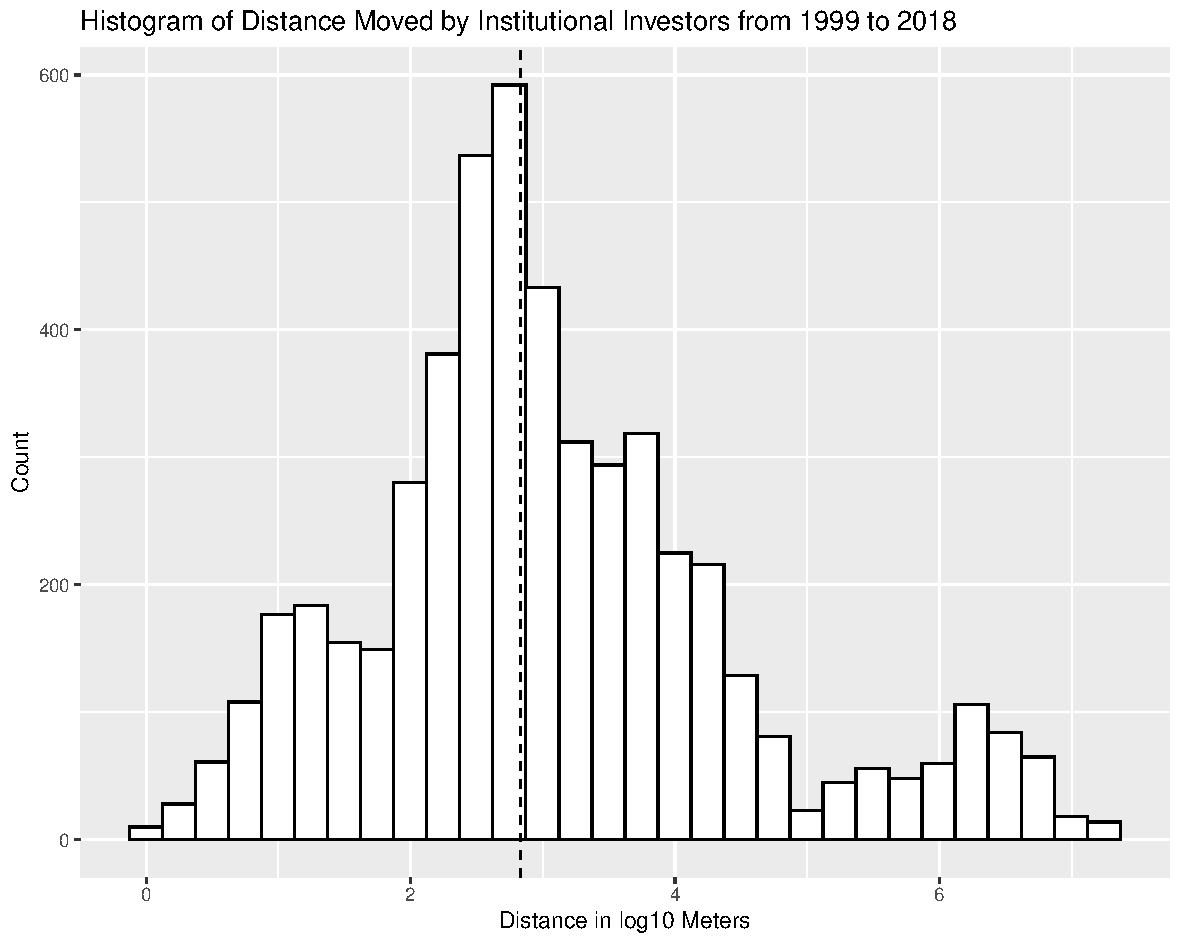
\includegraphics[width=0.7\linewidth]{Figures/ChapterIII/Distance_Moved_Histogram}
	\caption[Distance Moved by Firms]{Distance Moved by firms during the time period of 1999 to 2018 in Log10 meters.  The dashed vertical bar represents the median distance traveled of 680 meters and a mean distance of 269 040 meters (rounded to the nearest 10m).}
	\label{fig:distancemovedhistogram}
\end{figure}

A further cause for the widespread distribution of institutional investors in the United States is the historical legacy of US banking regulations.  The 10th Amendment of the US Constitution reserved banking regulations to the States, whereas the commerce clause gave the Federal government jurisdiction over interstate commerce.  This division in jurisdiction lead to the creation of a regime of regional banks rather than a small clique of national banks \citep{Calomiris2000}. Furthermore, the proliferation of State-managed employee pension funds ensures the existence of institutional investors outside of financially centred metropolitan areas such as New York, Boston, Chicago or San Francisco.  This remains the case despite the recent trend of outsourcing a sizable portions of pension funds into more opaque (and thus outside of the purview of 13F disclosure) and hopefully high yielding private placement deals \cite{lerner2019investing}. 



\subsection{Investors by Core-Based Statistical Area}


\nomenclature{CBSA}{Core-Based Statistical Area}
Core-Based Statistical Areas (CBSA) are a relatively recent geographical construct by the U.S. Office of Management and Budget with the goal of creating a set of nationally consistent geographies that are useful for tabulating and comparing statistics.  These areas consist of at least 1 core county with a population greater than 10 000 inhabitants, as well as all adjacent counties with substantial economic and social integration \citep{USCensusCBSAdef}.  The CBSA is a useful construct for comparing urban areas since it creates a more homogeneous unit of comparison between different urban areas in the United States, particularly since the USA has a disparate mix of regional sub-units such as New England townships and Louisiana parishes.  Furthermore, the CBSA is subdivided into either a Metropolitan Statistical Area (population greater than 50 000) or a Micropolitan Statistical Area (population less than 50 000).  

Figure \ref{fig:countbycbsalegal} illustrates the absolute count of institutional investors by CBSA.  As previously mentioned in the State breakdown of institutional investors in the previous section, the New York - Newark - Jersey City CBSA gains the largest absolute amount of new institutional investors by a considerable margin, and Figure \ref{fig:percentageofinvestmentfirmsbycbsa} shows a similar picture to Figure \ref{fig:precentagestate} in which New York sees a relative decline.  Due to the presence of a few investors in non-CBSA counties, the investors located outside of CBSA were added to figures \ref{fig:countbycbsalegal} and \ref{fig:percentageofinvestmentfirmsbycbsa}.  Of particular note is the rapid rise of investment firms outside of the USA during this time period.  Figure \ref{fig:percentageoffirmsbycbsa} is similar to figure \ref{fig:percentageofinvestmentfirmsbycbsa}, but with the absence of foreign investment firms. When comparing these graphs, the difference in slope trajectory when the number of foreign firms is removed from the baseline is remarkable.   At this scale, the relative density of investment firms still follows the same inverted U shape, with a peak on or about the first quarter of 2007.  

\begin{figure}[h]
	\centering
	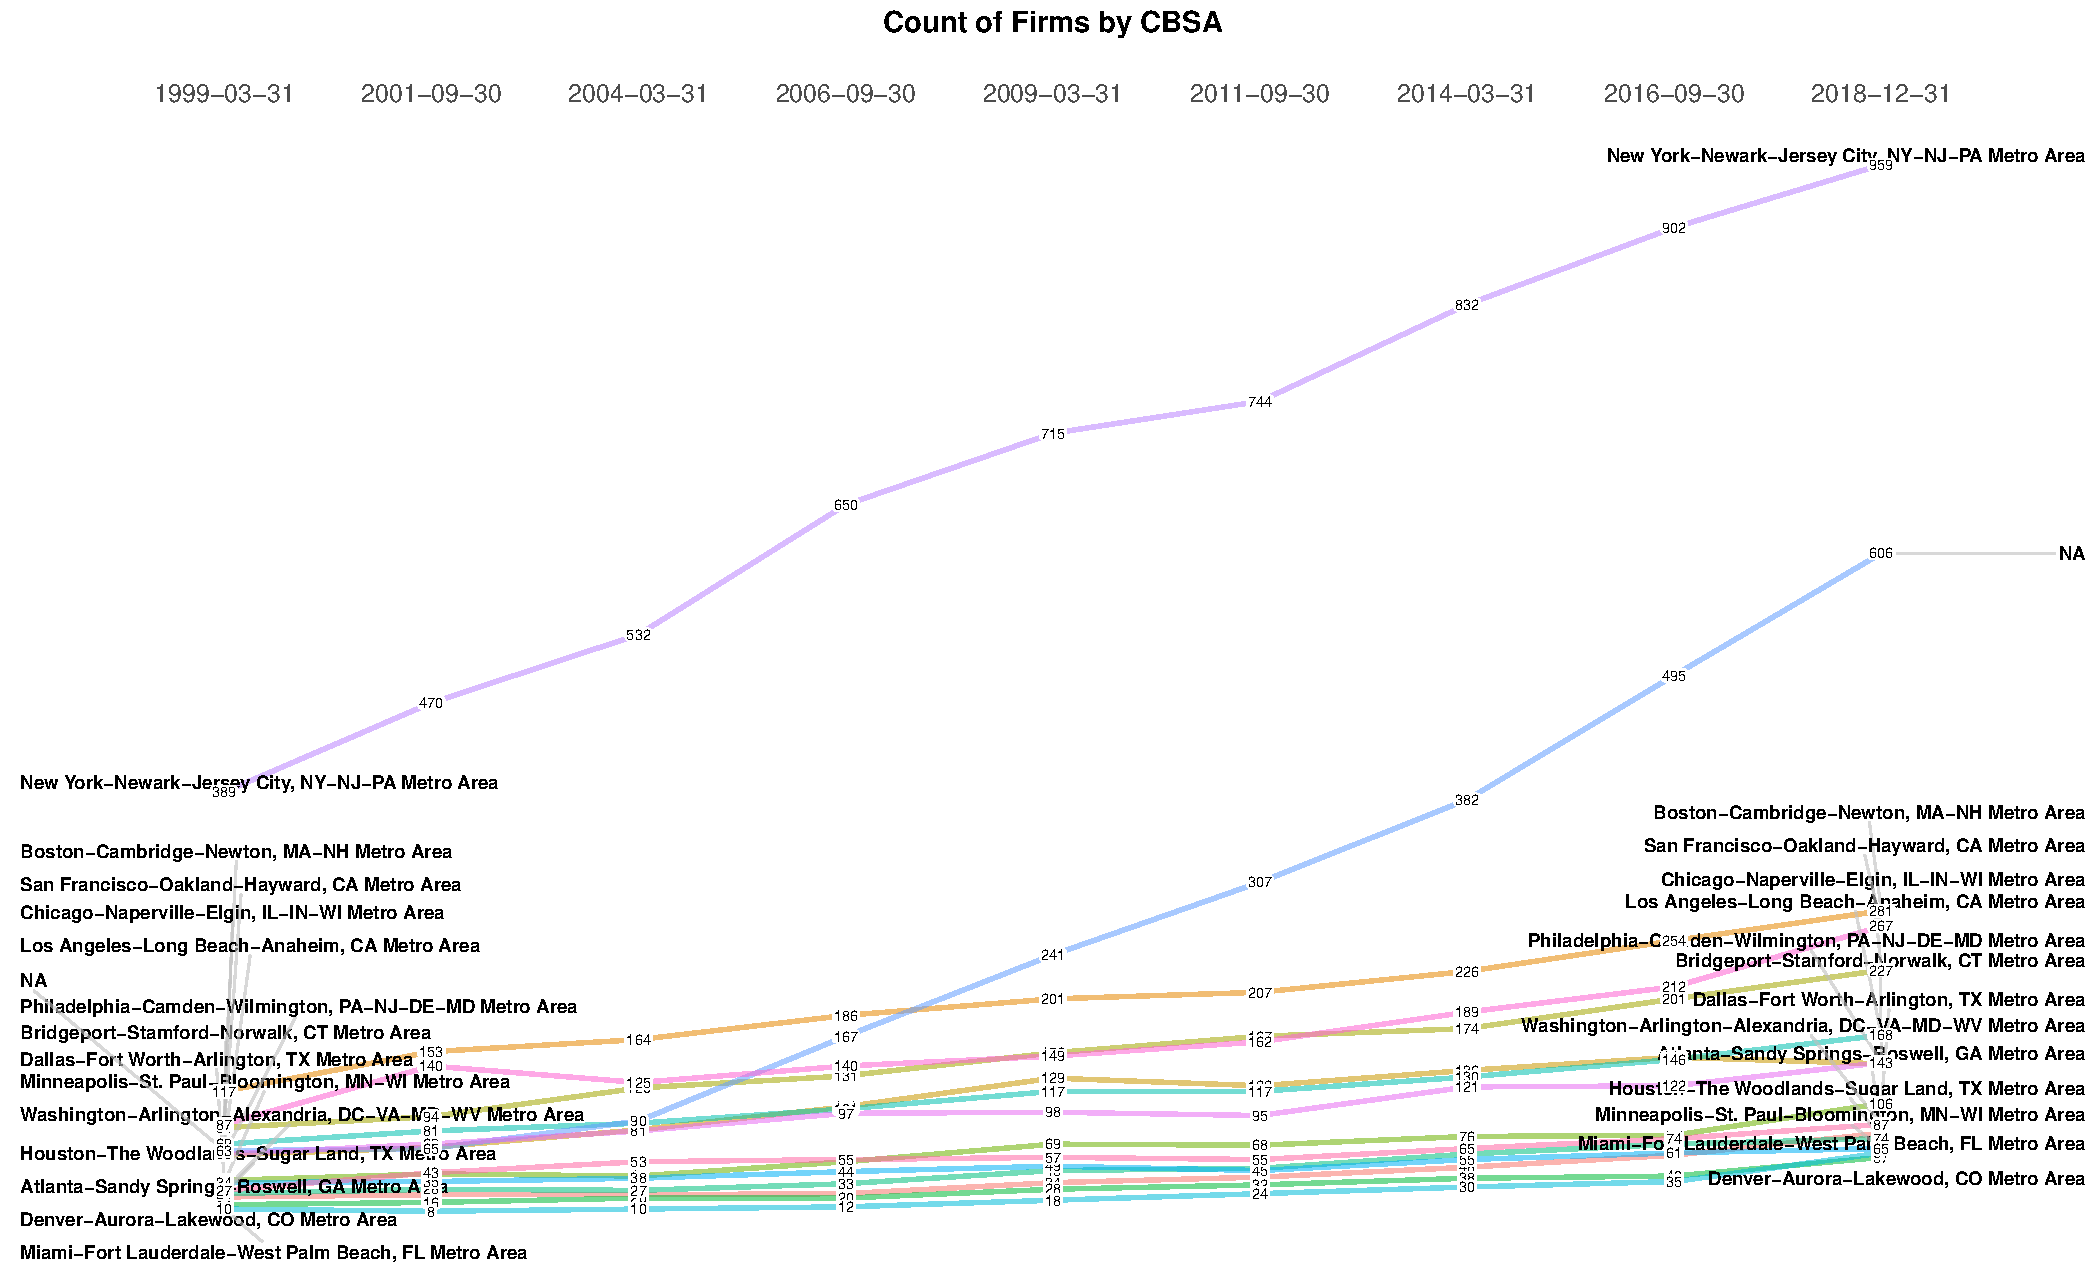
\includegraphics[width=1\linewidth]{Figures/ChapterIII/Count_by_CBSA_Legal}
	\caption[CBSA Legal]{Count of Institutional investors by Core-Based Statistical Areas for the period 1999 to 2018}
	\label{fig:countbycbsalegal}
\end{figure}


\begin{figure}[h]
	\centering
	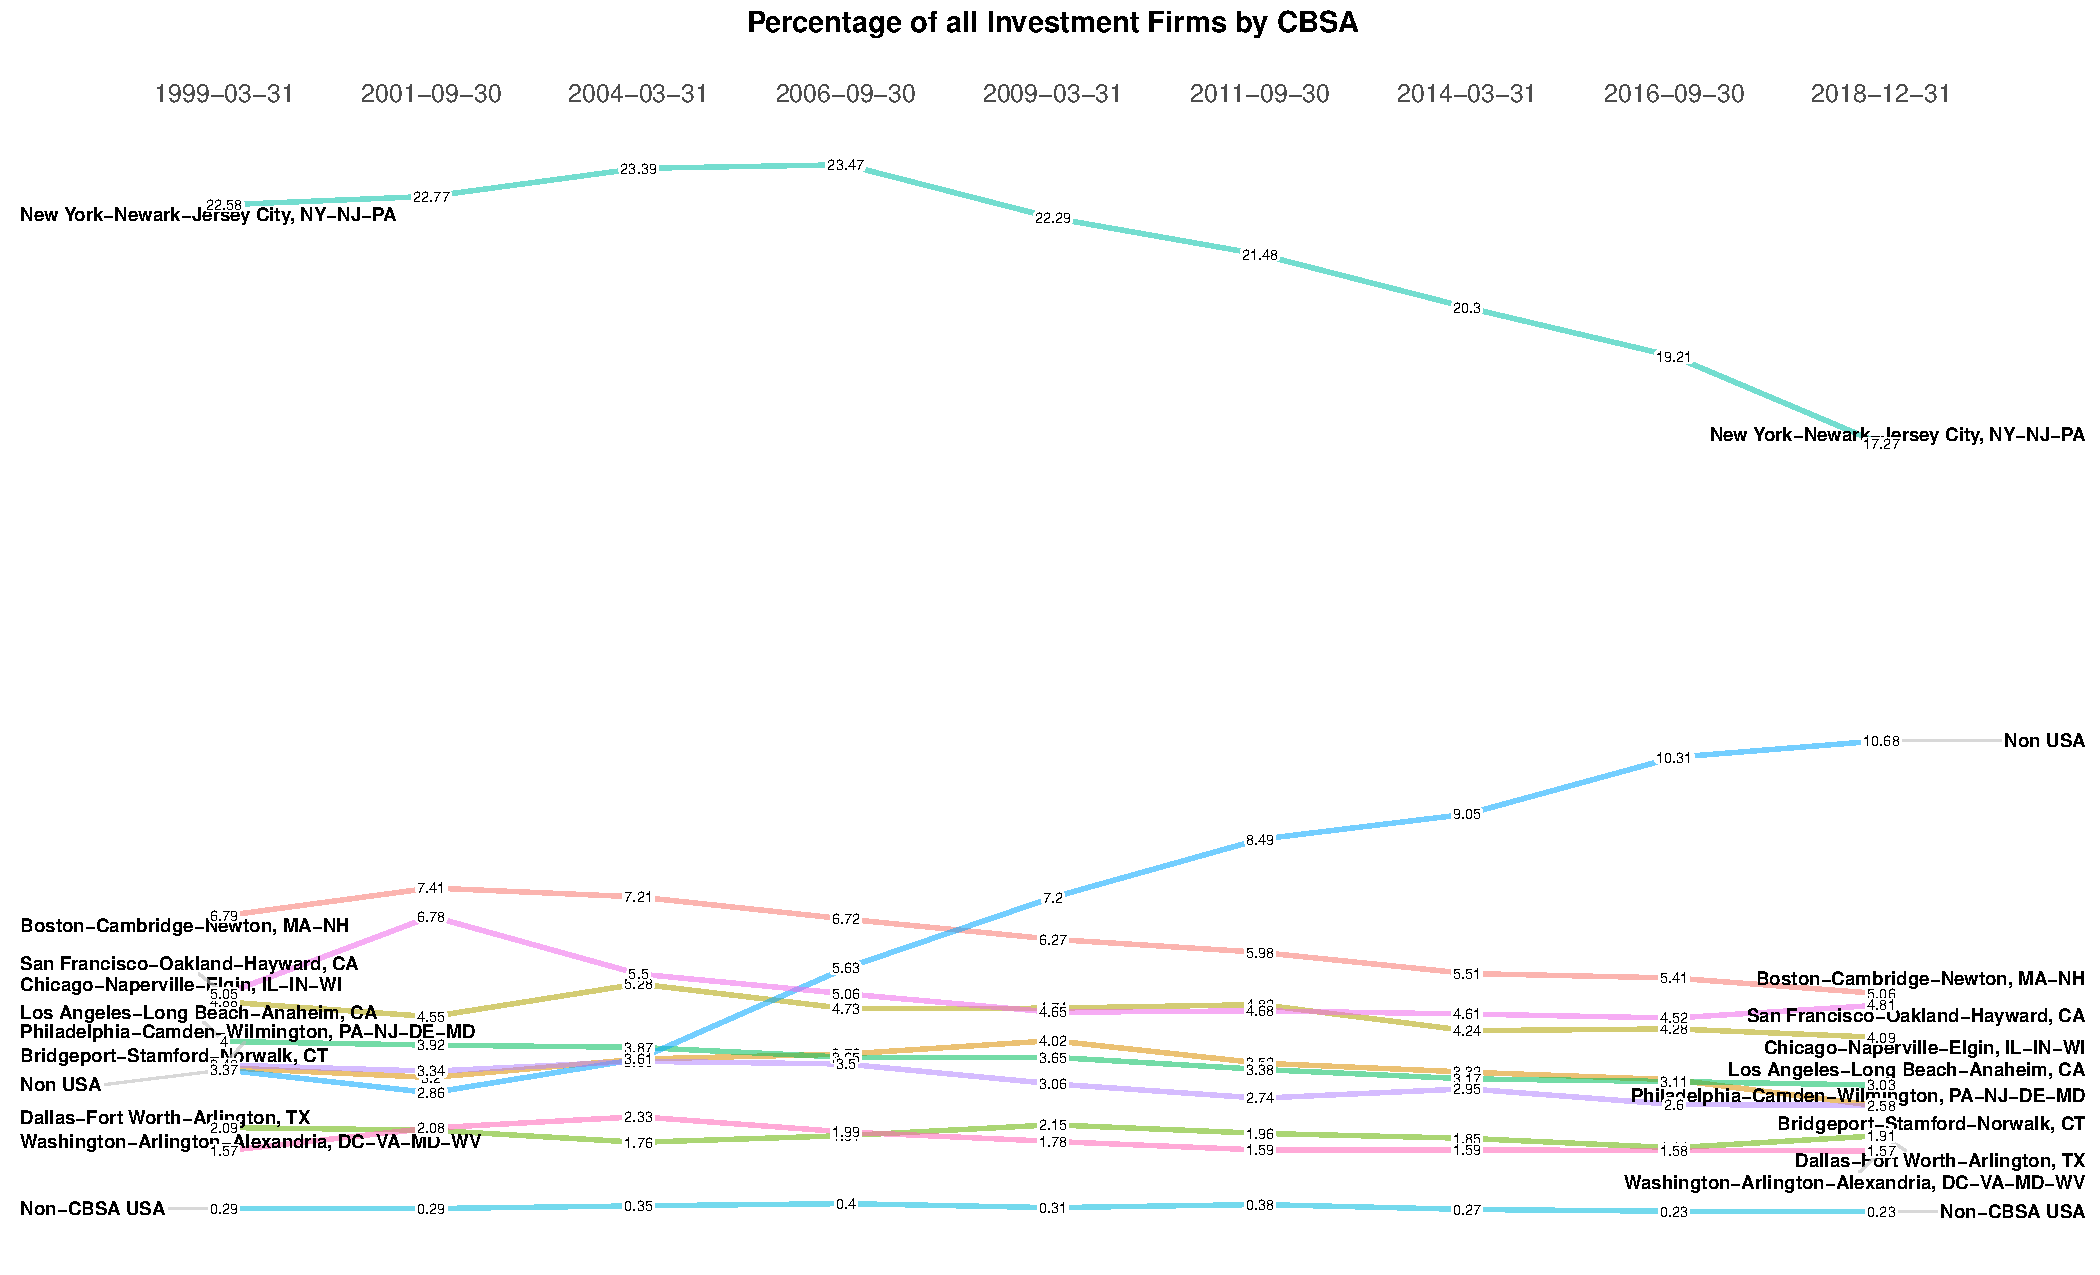
\includegraphics[width=1\linewidth]{Figures/ChapterIII/Percentage_of_Investment_Firms_by_CBSA}
	\caption[Precent Investment]{Share of Institutional investors by Core-Based Statistical Areas for the period 1999 to 2018}
	\label{fig:percentageofinvestmentfirmsbycbsa}
\end{figure}



\begin{figure}
	\centering
	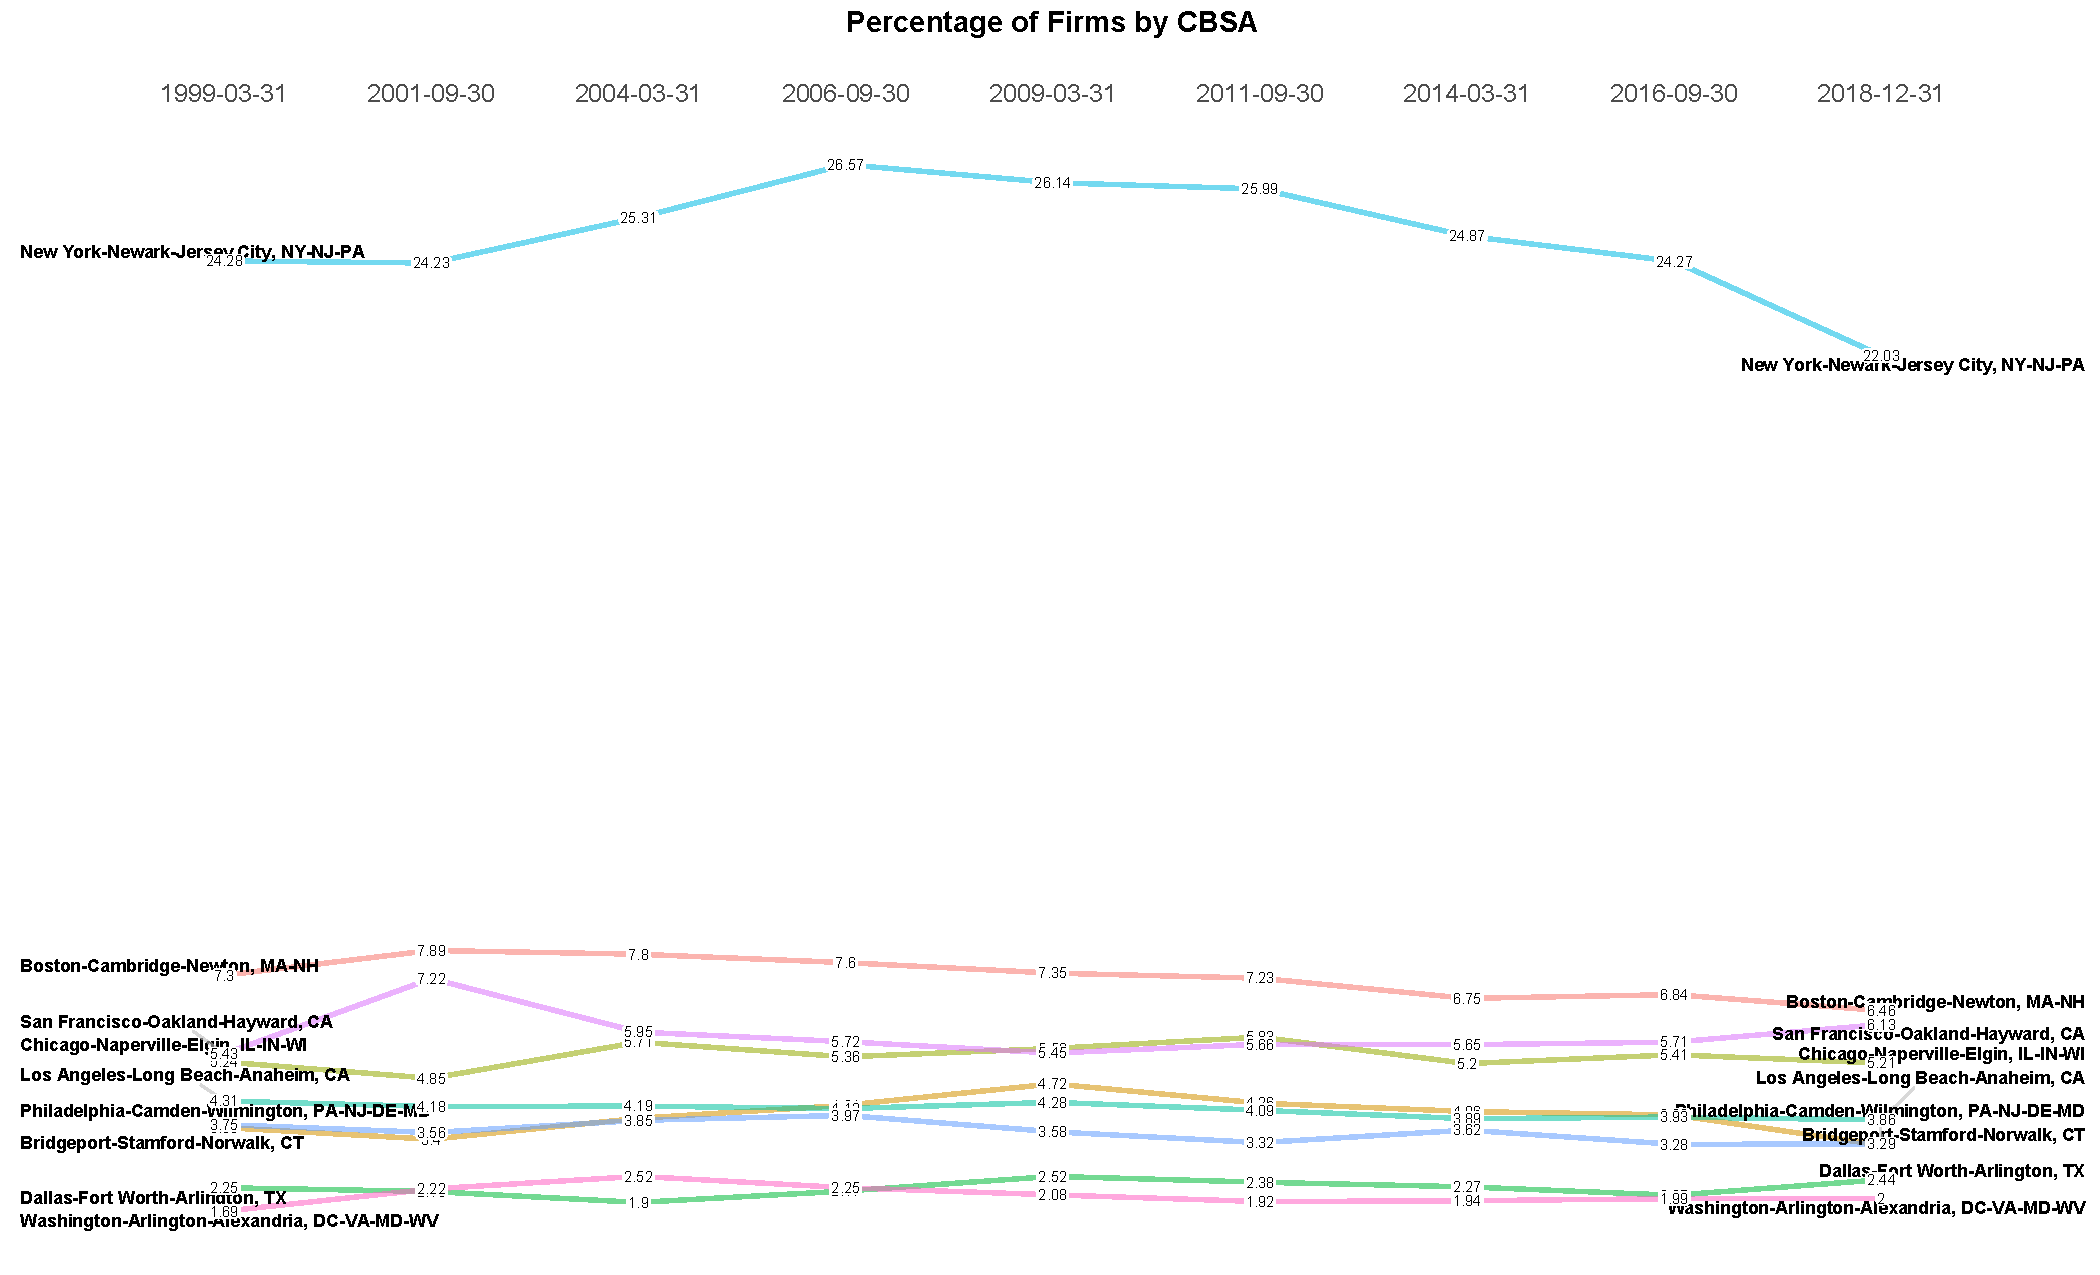
\includegraphics[width=1\linewidth]{Figures/ChapterIII/Percentage_of_Firms_by_CBSA}
	\caption[Percent by CBSA]{Percent by Share of Institutional investors by Core-Based Statistical Areas for the period 1999 to 2018}
	\label{fig:percentageoffirmsbycbsa}
\end{figure}



\subsection{Investors by County}
\label{investorsbycounty}
Diving further down the building blocks of US territorial systems, the next level down is that of the county. There are 3 242 counties and county equivalents in the USA, and its territories,  of which 2 707 do not have institutional investors during the entire period. In March of 1999, 2 972 counties do not host an institutional investor, however, by December 2018, the number of counties devoid of institutional investors falls to 2 786.  Considering that the USA added over 2 500 institutional investors during this period, this suggests that new institutional investors are attracted to counties with a pre-existing institutional investor population rather than filling-out empty counties.  



\begin{figure}
	\centering
	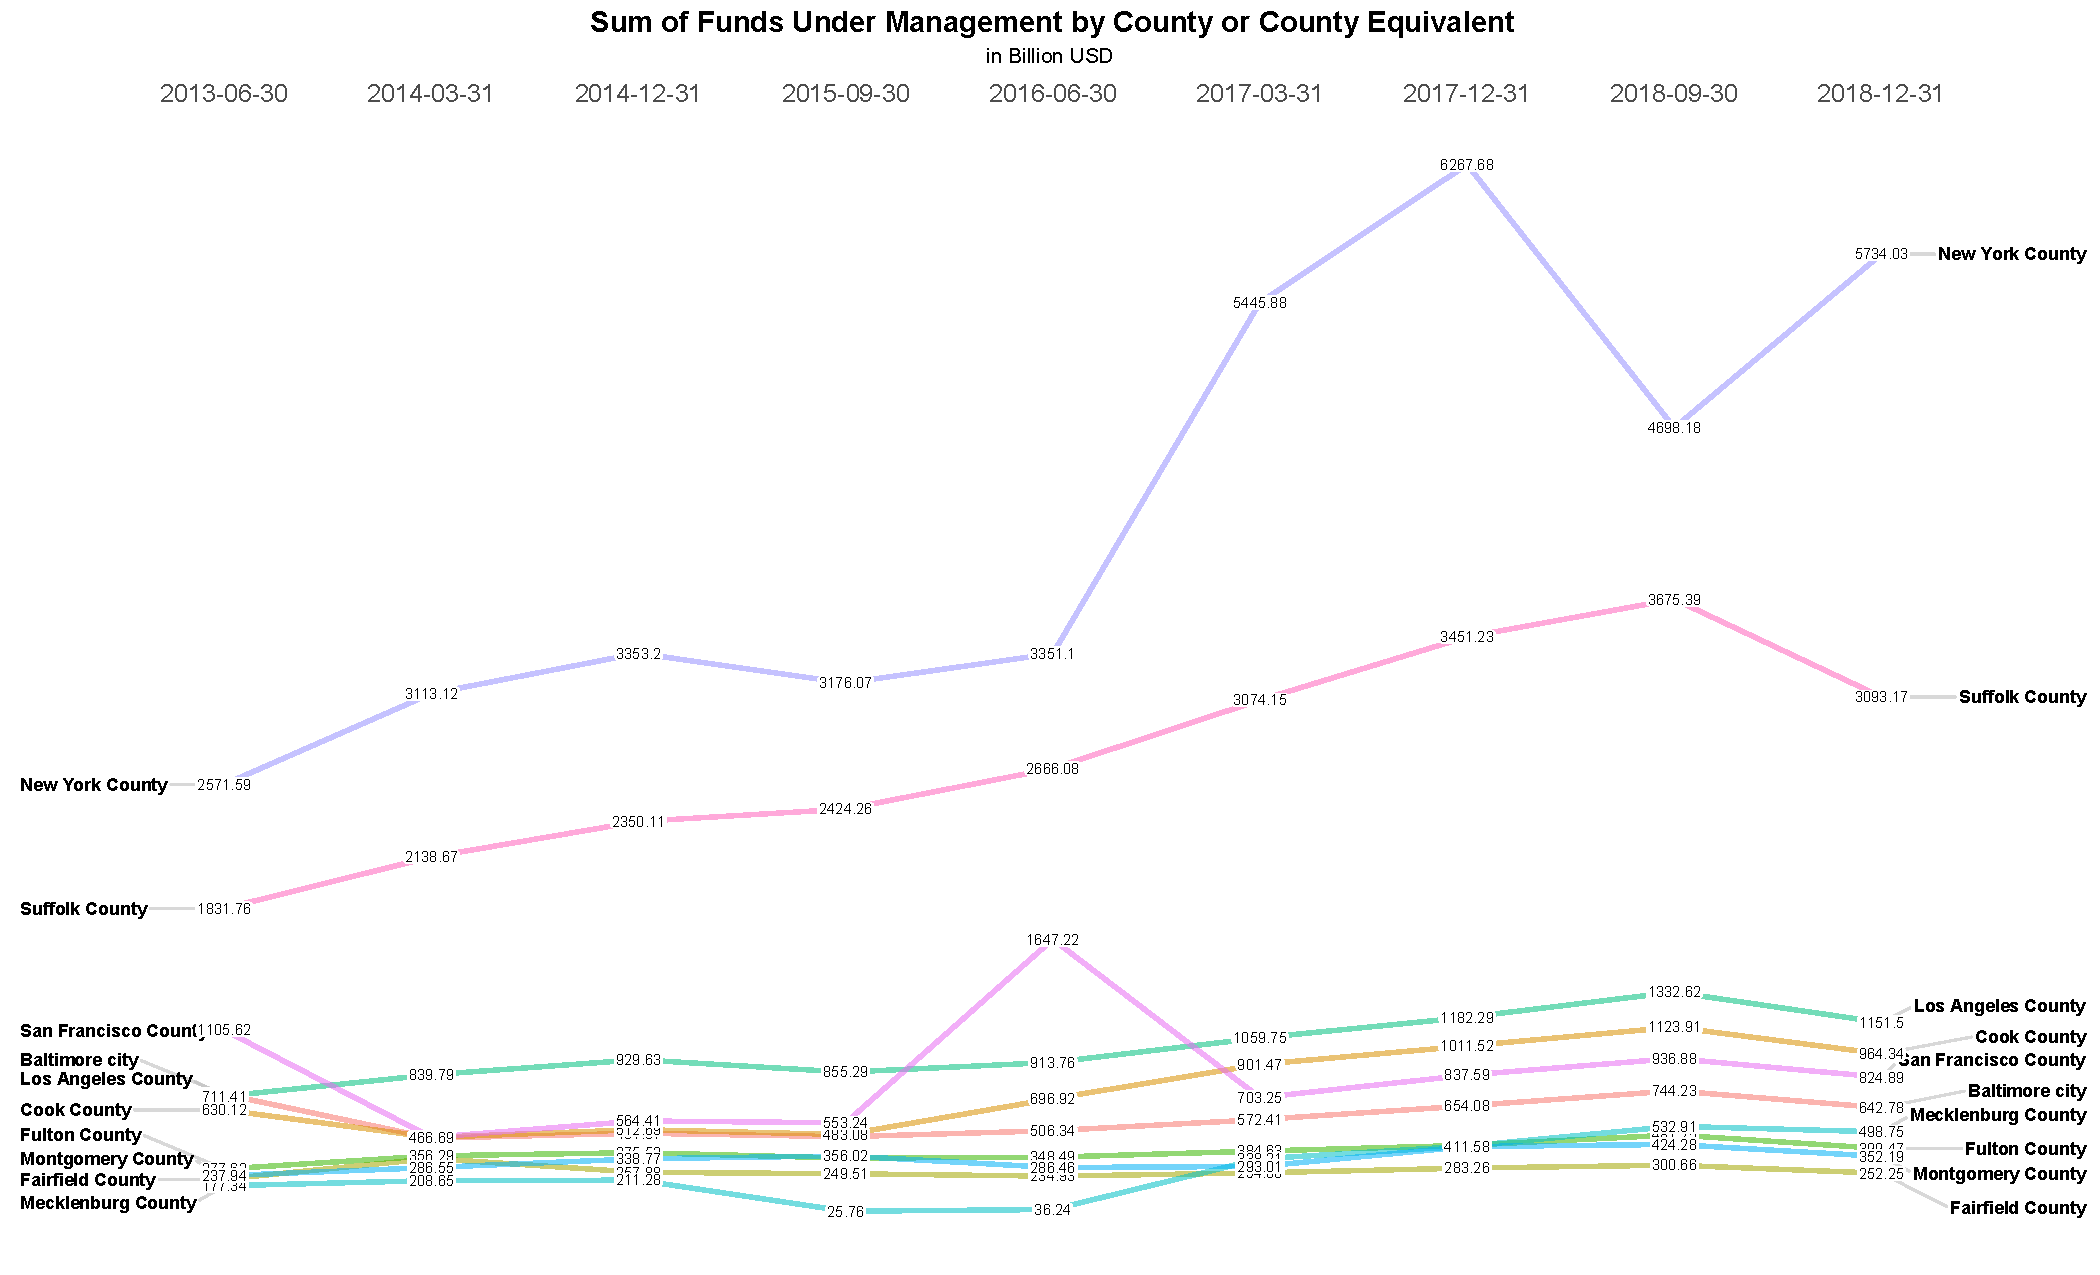
\includegraphics[width=1\linewidth]{Figures/ChapterIII/Sum_by_County}
	\caption[Sum by County]{Share of Institutional investors by county for the period 1999 to 2018}
	\label{fig:sumbycounty}
\end{figure}


\begin{figure}
	\centering
	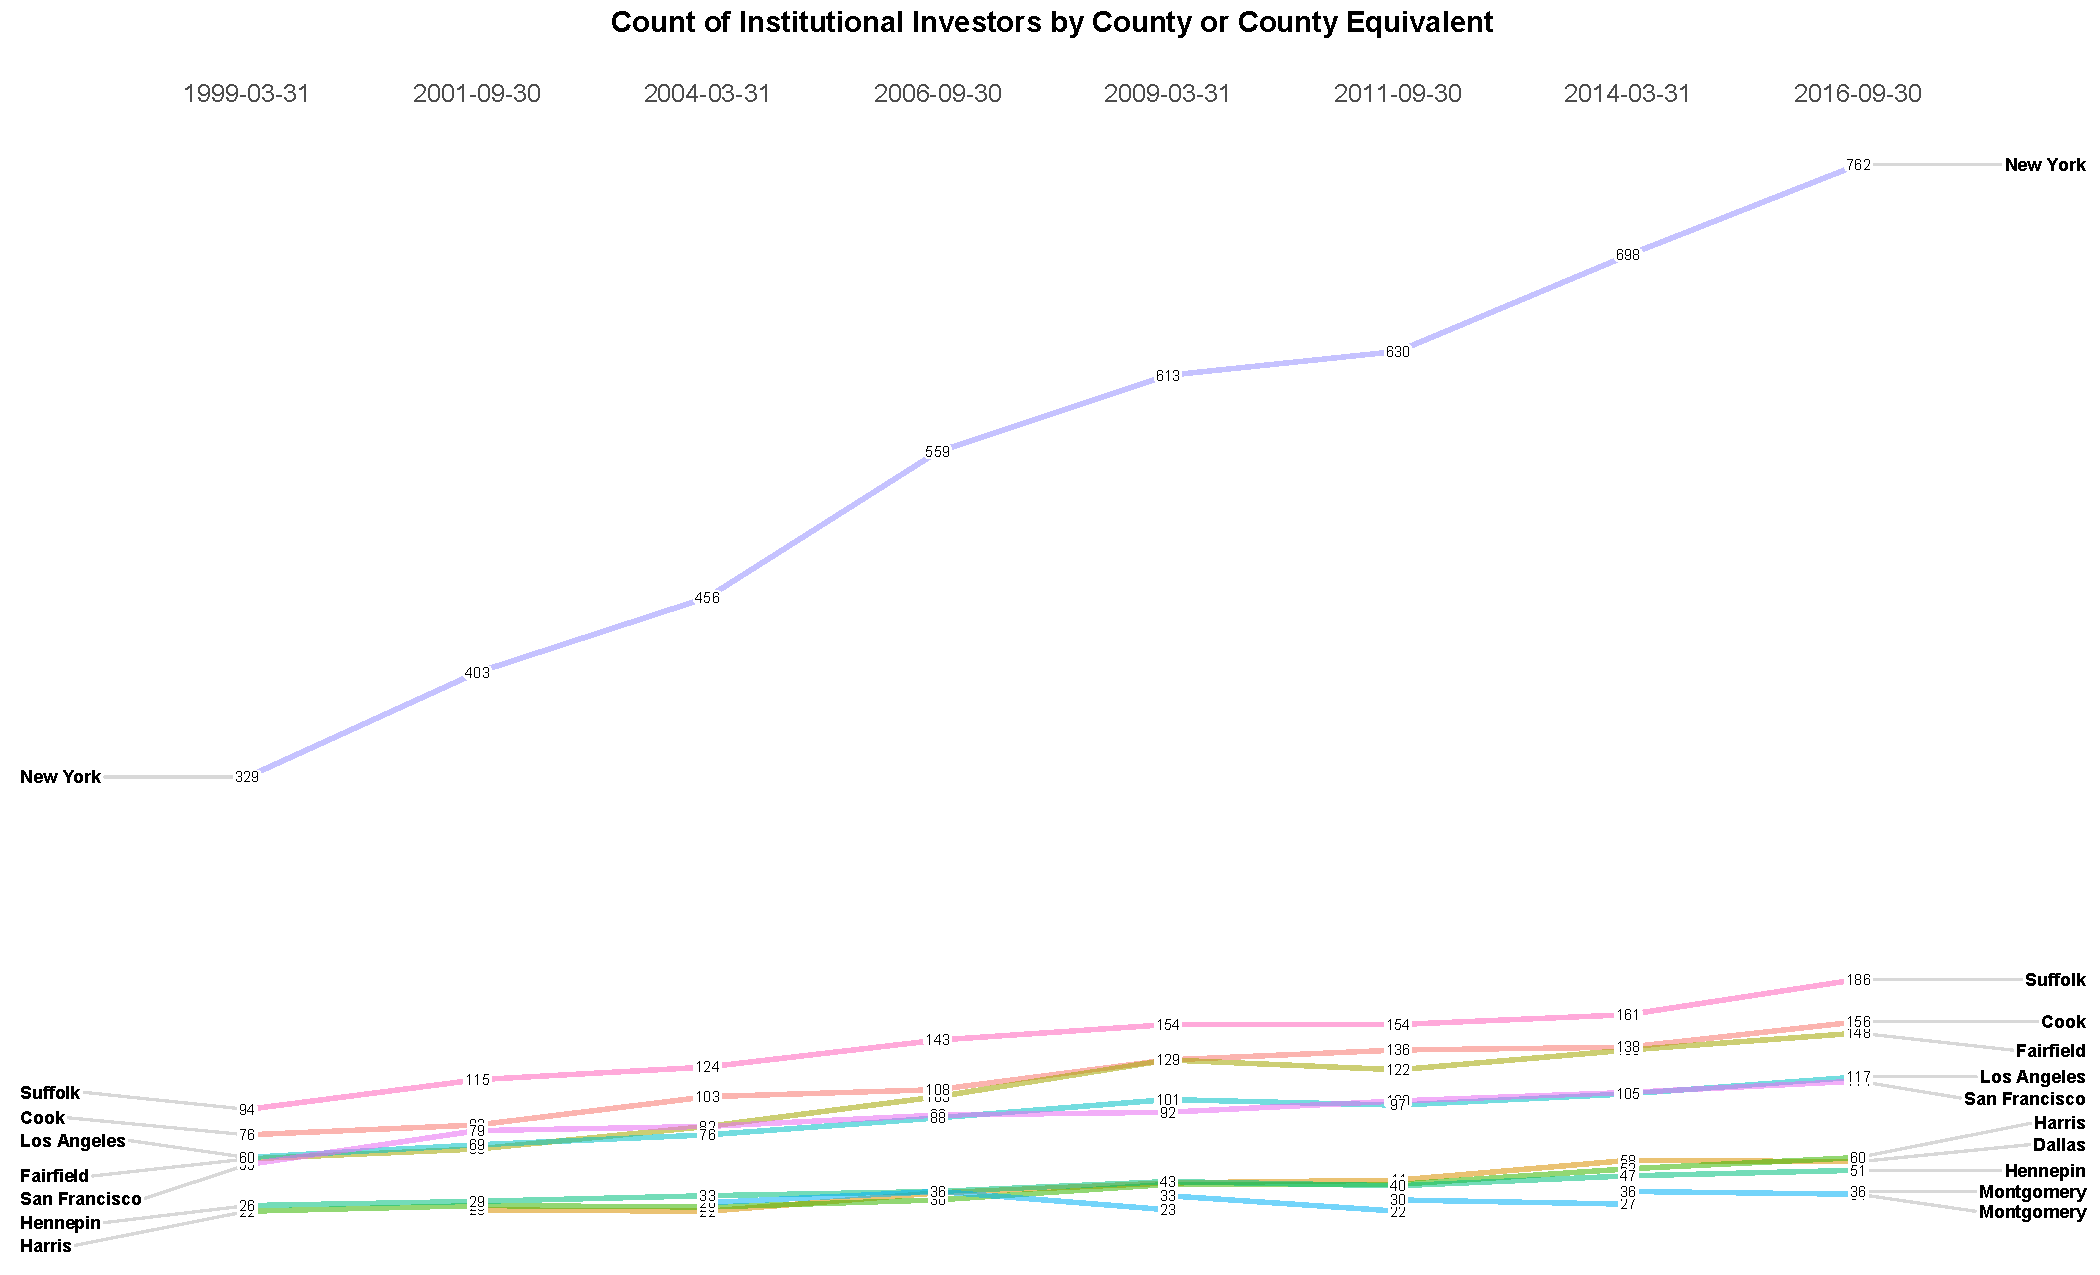
\includegraphics[width=1\linewidth]{Figures/ChapterIII/Count_by_County}
	\caption[Count by County]{Count Institutional investors by county for the period 1999 to 2018}
	\label{fig:countbycounty}
\end{figure}

This larger number of counties permits a different sort of analysis to be used: that of comparing Gini coefficients over time.  The Gini coefficient is a common descriptive statistic of inequality, with a value of 1 describing perfect inequality (one case having all of the measured variable) and 0 describing perfect equality (all cases having equal amounts of the variable). 

The Chow test is a statistical test developed by econometrician Gregory Chow for determining if two regression lines are equal.  Within the field of time series analysis, this is useful for determining if there is the presence of a structural break in the data.  	A look at figure \ref{fig:ginicounty} shows an increase in spatial dispersion over time.  Using a Chow test  (Figure \ref{fig:Chow Test}) to find the change in linear trend of the Gini coefficient indicates that there is a breakpoint in trend on June 30th, 2011  \citep{Chow1960}.  This is much later than the breakpoints mentioned earlier when looking at the concentration of firms in States and CBSAs. 	This can be somewhat explained by the Gini coefficient being more sensitive to areas going from 0 to 1 than say 15 to 16.  




\begin{figure}[h]
	\centering
	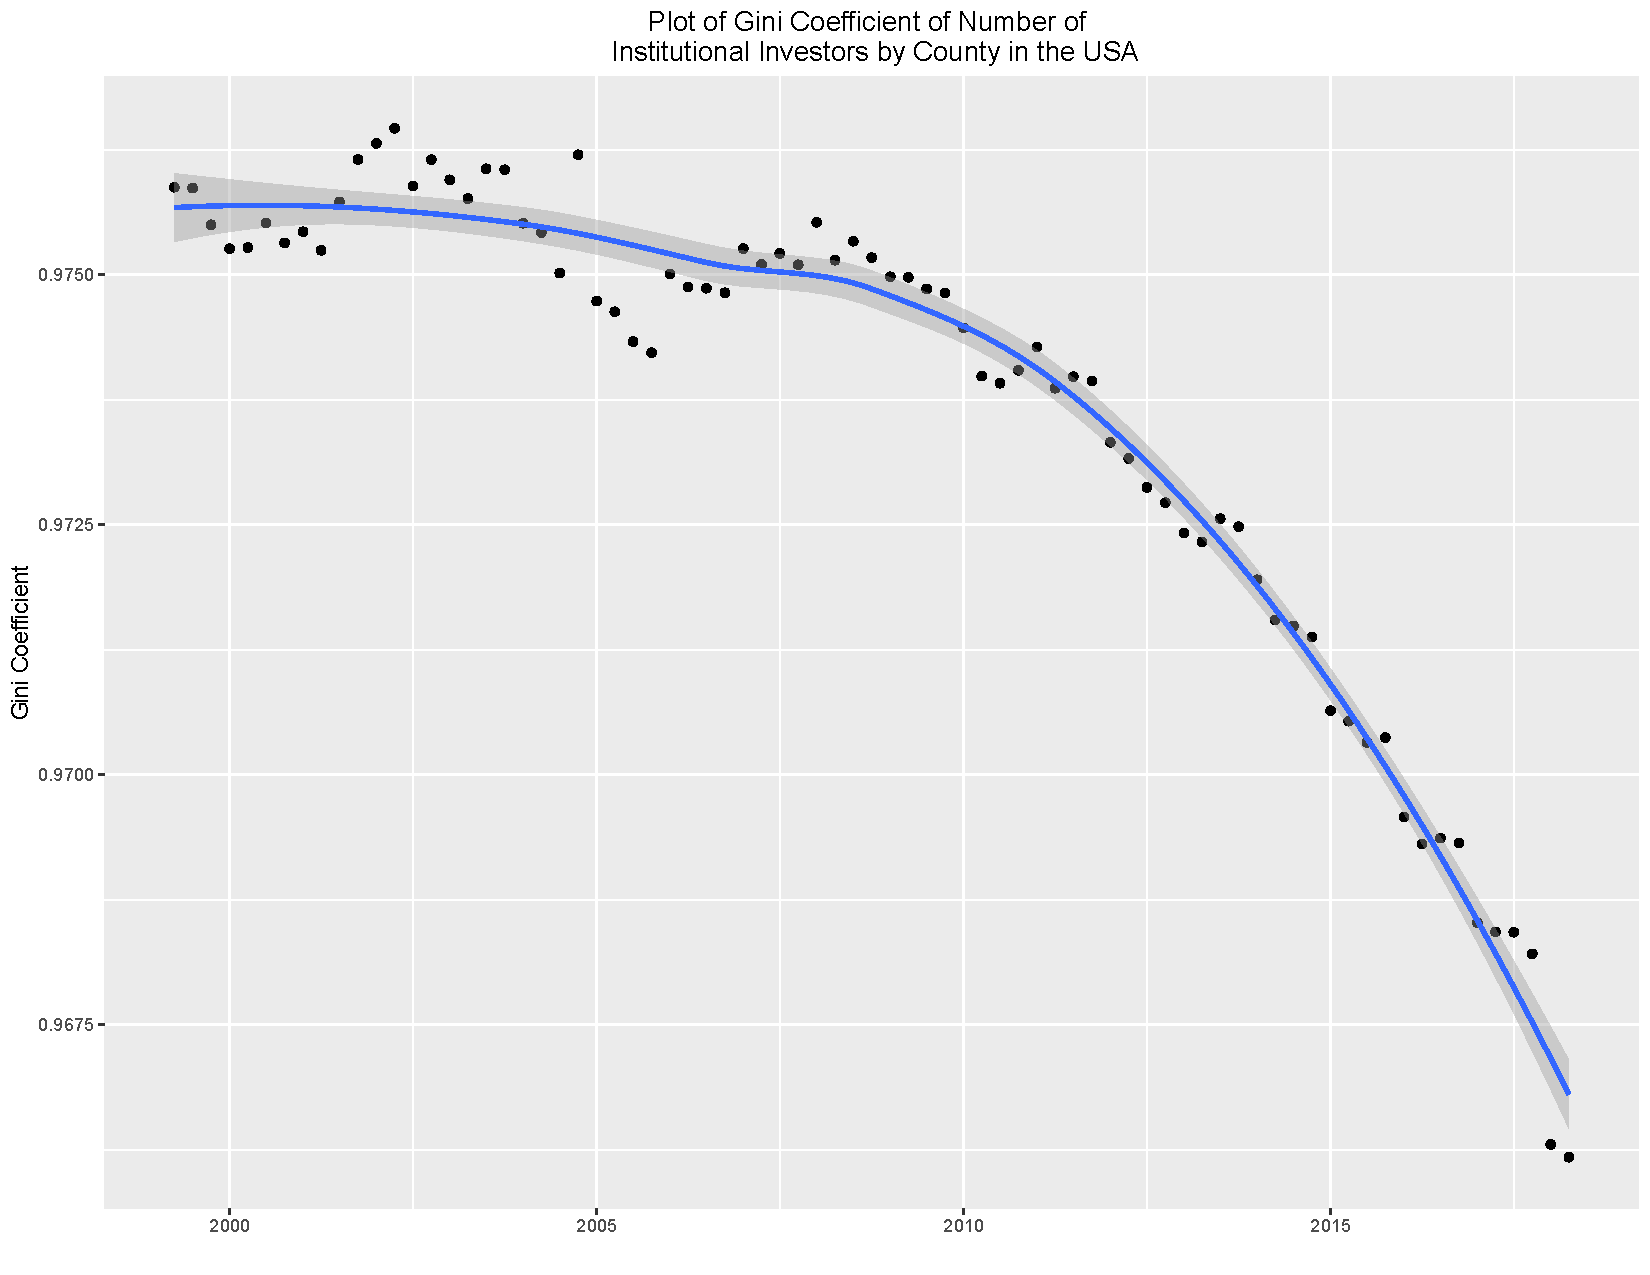
\includegraphics[width=1\textwidth]{Figures/ChapterIII/GINI_County}
	\caption[Gini Coefficent of US County Count]{Gini Coefficent of US County Count}
	\label{fig:ginicounty}
\end{figure}


\begin{figure}[h]
	\centering
	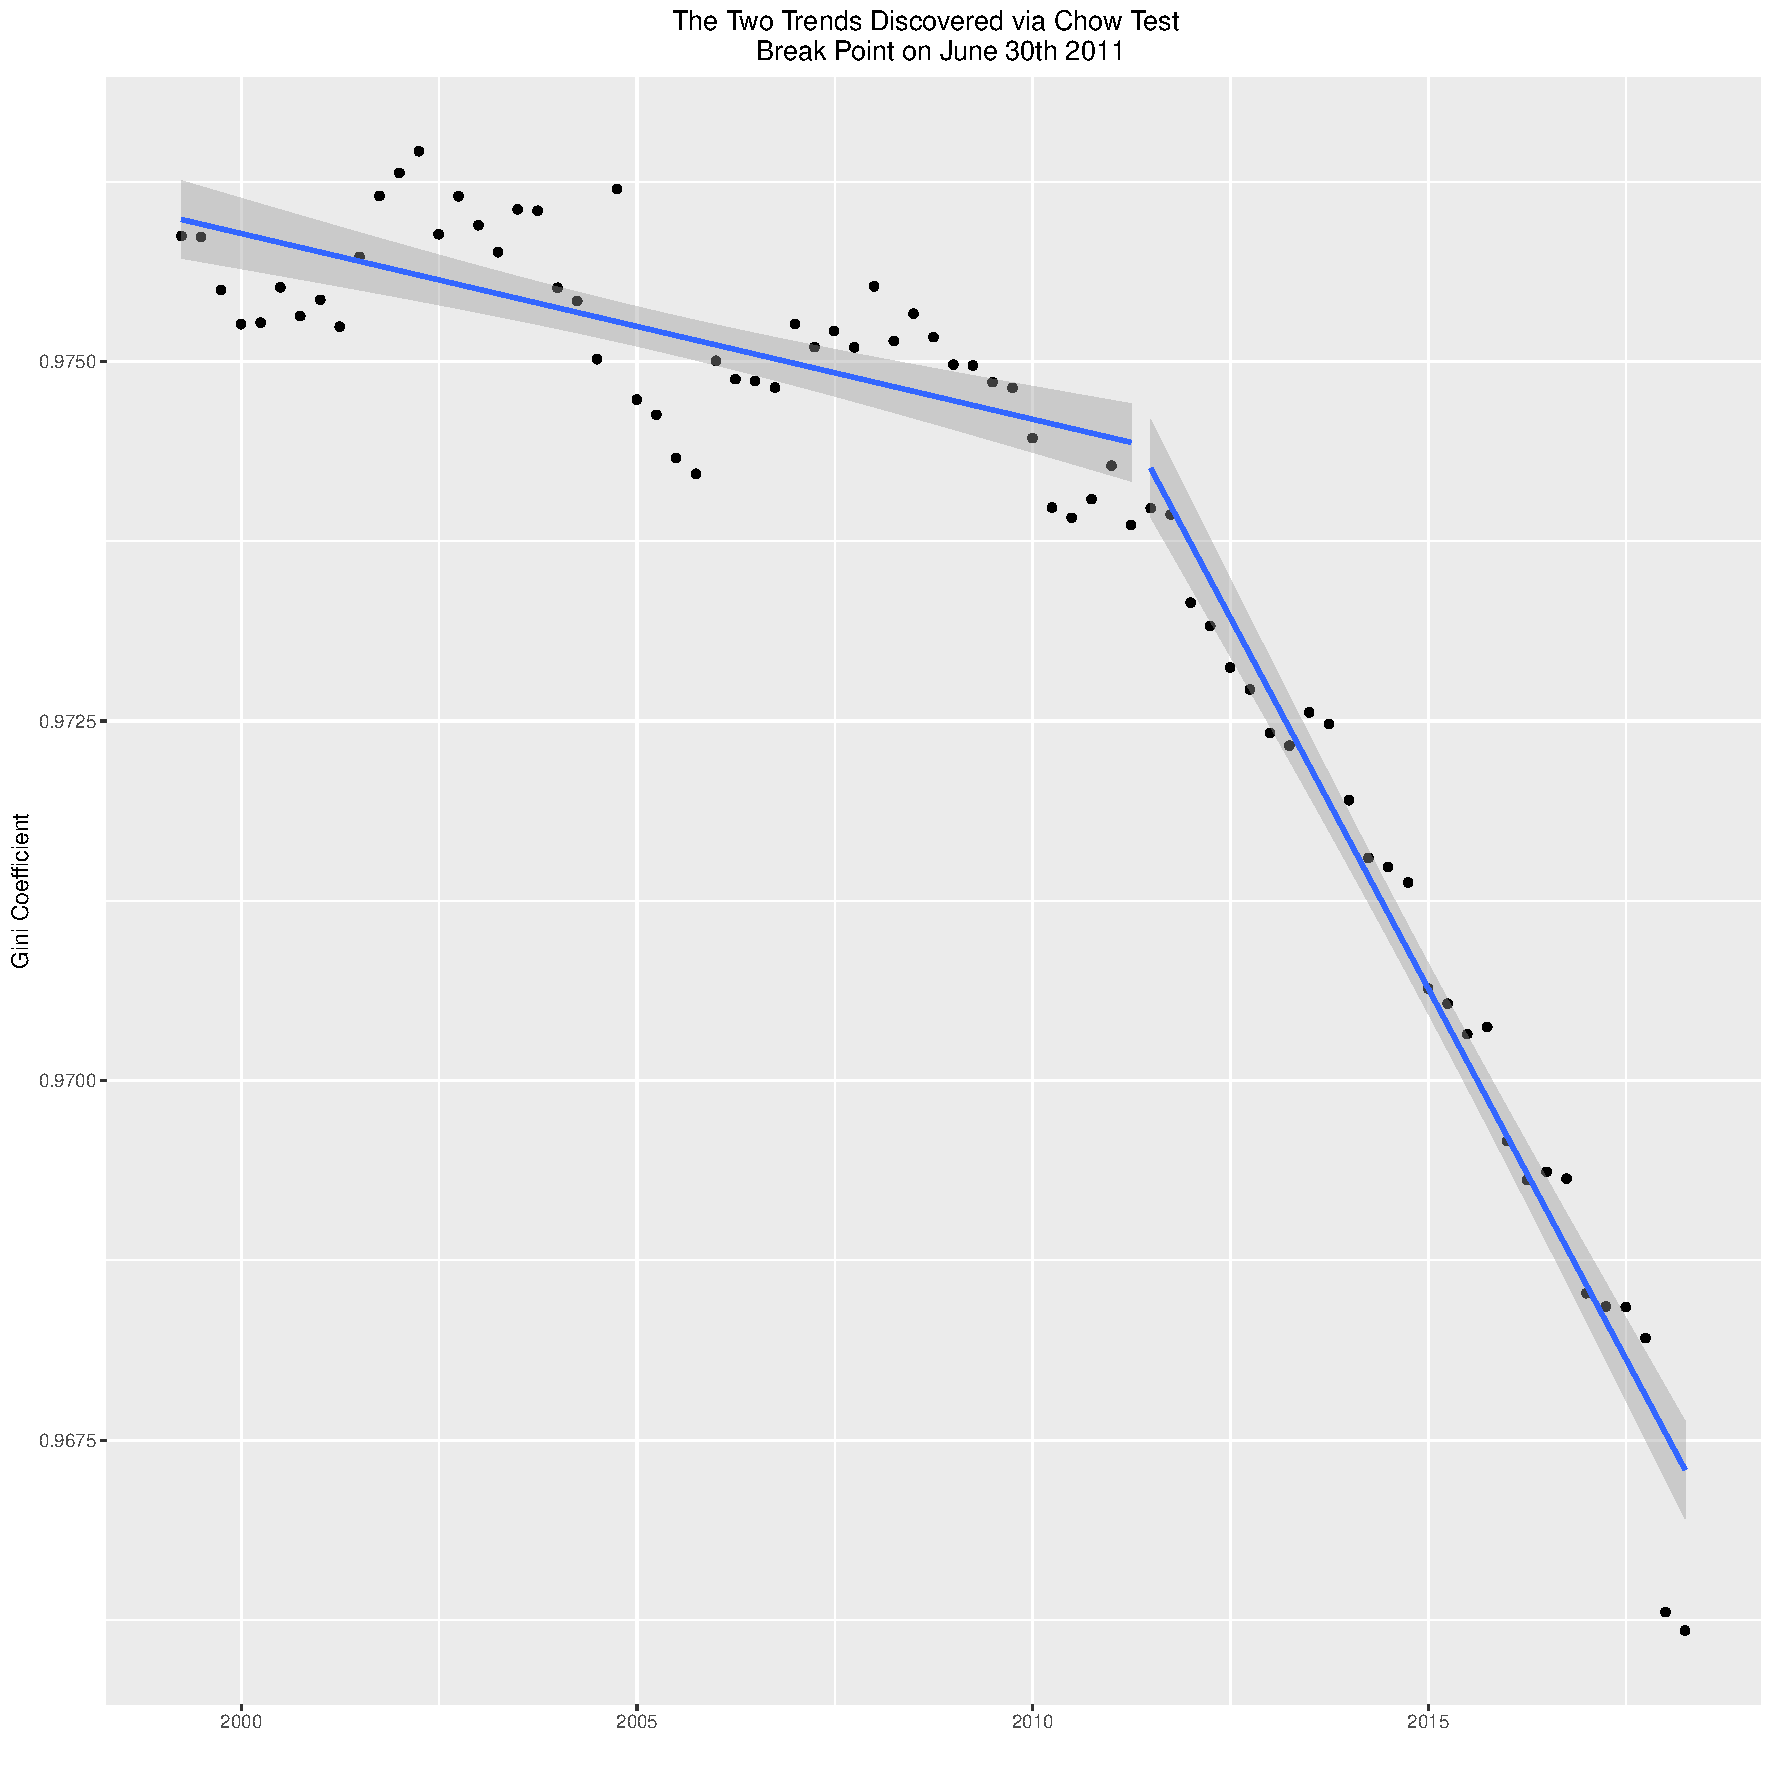
\includegraphics[width=1\textwidth]{Figures/ChapterIII/ChowTest.pdf}
	\caption[Chow Test Result]{Result of Chow test.  Breakpoint on June 30th 2011}
	\label{fig:Chow Test}
\end{figure}

\subsection{By County Urban Intensity Index}

Counties (and their equivalents) are important building blocks in the American territorial administration.  However, not all counties are created equal.  For example, Los Angeles County in California has a population approaching 10 million people, whereas rural counties such as Loving County in Texas contains less than 200 inhabitants \citep{USCensus13}.  In the field of health geography and epidemiology, rural-urban divide can play a role in predicting health outcomes.  The National Center for Health Statistics devised a classification scheme for all US counties that can be used as a proxy for the degree of urban surface area in each county \citep{national2014urban}. This classifies counties into one of 6 different categories.
\begin{enumerate}
	\item Metropolitan Categories:
	\begin{enumerate}
		\item \textbf{Large Central Metropolitan counties} (Category 1) are counties in Metropolitan Statistical Areas (MSAs) with at least 1 million inhabitants, and one of the following characteristics: 
		\begin{enumerate}
			\item contain the entire population of the largest principal city of the MSA, or 
			\item are completely contained within the largest principal city of the MSA, or 
			\item contain at least 250,000 residents of any principal city in the MSA.
		\end{enumerate}
		Examples: New York County New York\footnote{Coterminous with Manhattan Borough in the City of New York}, Bronx County New York, Los Angeles County California, Cook County Illinois. 
		
		\item  \textbf{Large peripheral metro counties} (Category 2) are counties in a MSA with a population greater than or equal to 1 million, but do not qualify as category 1 county.  
		
		Examples: Orange County New York, San Mateo County California
		
		
		\item \textbf{Medium metro counties} (Category 3)are counties in MSA with a population greater than 250,000 but less than one million in population.
		
		Example: Fresno County California, New London County Connecticut
		
		\item \textbf{Small metro counties} (Category 4)are counties in MSAs with populations greater than 50,000 but less than 250,000 in population.
		
		Example: Yuma County Arizona, Franklin County Vermont
		
	\end{enumerate}
	\item	Non-metropolitan Categories:
	\begin{enumerate}
		\item \textbf{Micropolitan counties} (Category 5) are counties in a micropolitan statistical area
		
		Example:  Juneau City and Borough Alaska, Talladega County Alabama
		
		\item \textbf{Noncore counties} (Category 6) are counties that do not contain a micropolitan statistical areas
		
		Example: Loving County Texas, Denali Borough Alaska
	\end{enumerate}
\end{enumerate}


This categorisation of counties gives insight into the type of region the new institutional investors prefer. As predicted by Quaternary Location Theory, it is hardly surprising that institutional investors are primarily found in large urban areas. This was also hinted in Figures \ref{fig:countbycbsalegal},  \ref{fig:percentageofinvestmentfirmsbycbsa}, and \ref{fig:percentageoffirmsbycbsa}, where it shows that the majority of investors are clustered around the topmost cities in the USA urban hierarchy.  Therefore it should be of no surprise that Figure \ref{fig:changeinrelativenumberruralurban} indicates that 95 percent of institutional investors are located in Metropolitan counties, and that the share of investors in Micropolitan counties is quite stable over time.  The largest change is that category 2 counties see an increase in market share, which mostly comes at the expense of category 1 counties. This provides evidence that while downtown areas are slightly less attractive to investors, going for bargain basement land costs is also not a preferred strategy, or else we would see an uptick over time in the counts of category 5 or category 6 counties.  While the relative gains of category 2 counties are impressive, one should not loose sight of the fact that the largest absolute growth in the number of institutional investors occurs in category 1 counties (Figure \ref{fig:changeinabsolutenumberruralurban}).     

It should be noted that the drop in number of firms in the aftermath of the 2008 great financial crisis is of nearly equal proportion in all categories of counties (Figure \ref{fig:changeinrelativenumberruralurban}).  Yet it is quite evident when looking in absolute numbers of extant institutional investors (Figure \ref{fig:changeinabsolutenumberruralurban}) that category 1 counties take a longer period of time to reestablish their number of investors.  

This growth in secondary counties in a conurbation may also hint a second phenomenon, such as an increase preference/and or availability of suburban office space in response to the expense of downtown offices.  \cite{Pohl2004} examines the remaining stock of real-estate in Manhattan after the terrorist attack on the World Trade Center and concludes that the destruction of World Trade Center Buildings 1, 2 and 7, as well as the damage on the other buildings essentially removed nearly a quarter of Manhattan's tier 1 and 2 office space from the market, and that the resulting scramble for office space tightened Manhattans' office market, spilling over into the other 4 boroughs as well as suburban New York, New Jersey, and Connecticut.  



\begin{figure}
	\centering
	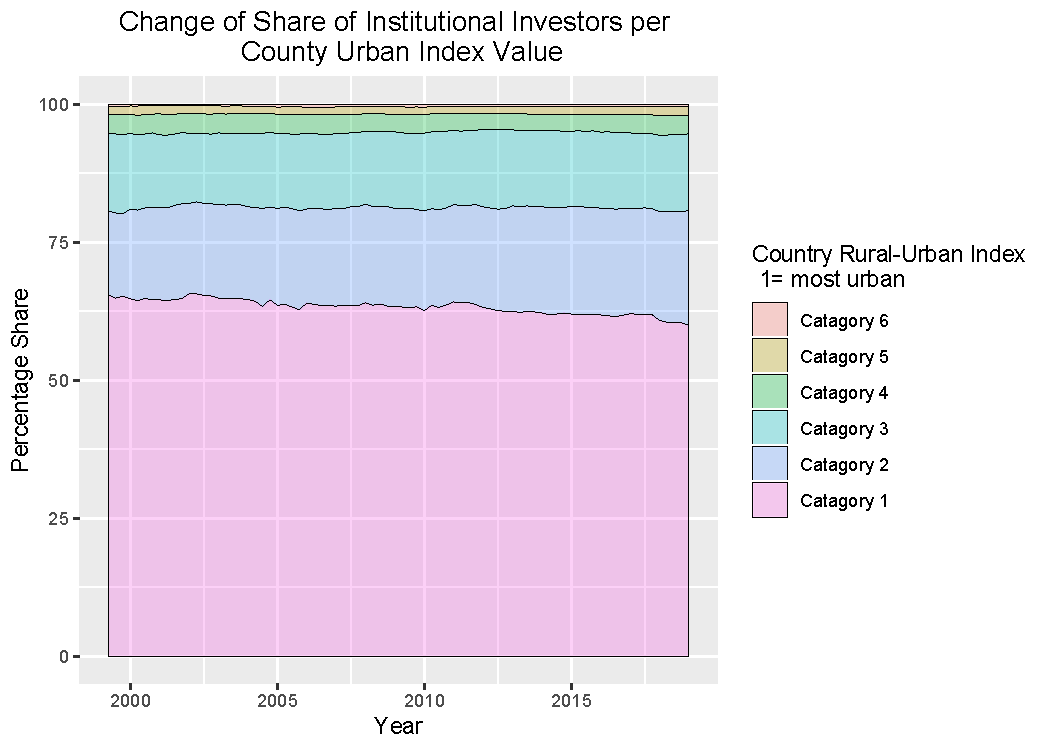
\includegraphics[width=1\linewidth]{Figures/ChapterIII/ChangeInRelativeNumberRuralUrban}
	\caption[Relative Numbers of Institutional Investors Over Time by County Urban-Rural Index]{Percentage Share of firms by County Urban Index Value from 1999 to 2018}
	\label{fig:changeinrelativenumberruralurban}
\end{figure}

\begin{figure}
	\centering
	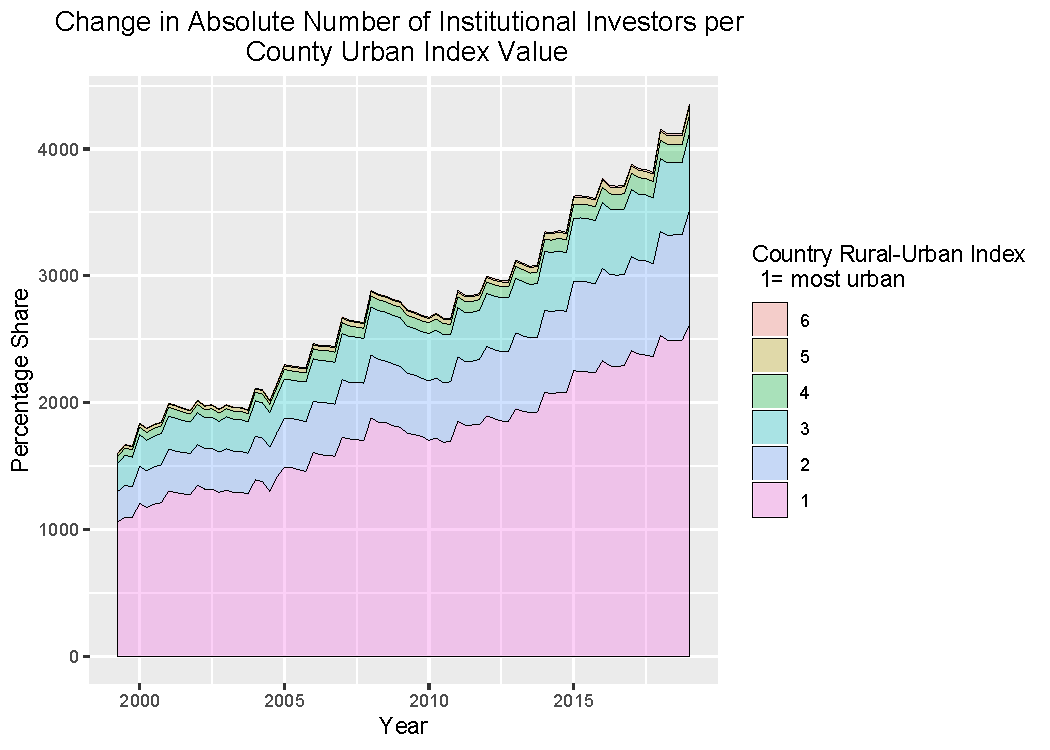
\includegraphics[width=1\linewidth]{Figures/ChapterIII/ChangeInAbsoluteNumberRuralUrban}
	\caption[Absolute Numbers of Institutional Investors Over Time by County Urban-Rural Index]{Count of firms by County Urban Index Value from 1999 to 2018}
	\label{fig:changeinabsolutenumberruralurban}
\end{figure}


\subsection{Investors By Region}

A way to reconcile the decline in market share of the New York region in Figures \ref{fig:precentagestate}, \ref{fig:percentageofinvestmentfirmsbycbsa}, and \ref{fig:percentageoffirmsbycbsa}  with Figures \ref{fig:changeinrelativenumberruralurban} and \ref{fig:changeinabsolutenumberruralurban} is to ask if the traditional definition of State or CBSA is too narrow, and that the declines may be partially explained by the modifiable area problem (MAP). \nomenclature{MAP}{Modifiable Areal Problem} The MAP is a source of statistical bias in geography-based data aggregation, since boundaries on reporting areas can have an outsized influence \citep{Fotheringham1991}.  A common extreme case of the MAP is gerrymandering, in which a political party can gain more seats relative to its vote share by controlling how the votes are aggregated into different districts.  In this case, all of the levels of aggregation seen so far (State, CBSA and County) fail to holistically capture Megaregions in the USA, and in particular the Boston-New York-Washington (Bos-Ny-Wash) megaregion  \citep{lang2007america}. While it may not fully encompass the Bos-Ny-Wash, the US Census Bureau's Region\footnote{\url{https://www2.census.gov/geo/pdfs/maps-data/maps/reference/us_regdiv.pdf} for a map listing the geographies encompassed by the different regions} does a good approximation of this.  

\label{Atlanta}

\nomenclature{Bos-Ny-Wash}{Boston-New York-Washington DC Megaregion}

In the case of Figure \ref{fig:Percentage_firms_Region_USA}, the decline of the North East is much slower than one would expect from previous graphs, mostly due to the inclusion of the south shore of Connecticut and the North shore of New Jersey.  


Increases in the number of Southern-based investors lies mainly in the growth of firms located in the DC/Arlington Virginia region, as well as Atlanta. With regards to the decline of the Mid-West, as mentioned previously, this is more of a relative decline than an absolute decline, for while it started the study period with 321 (20\%) institutional investors and ended with 728 (17.6\%).


\begin{figure}
	\centering
	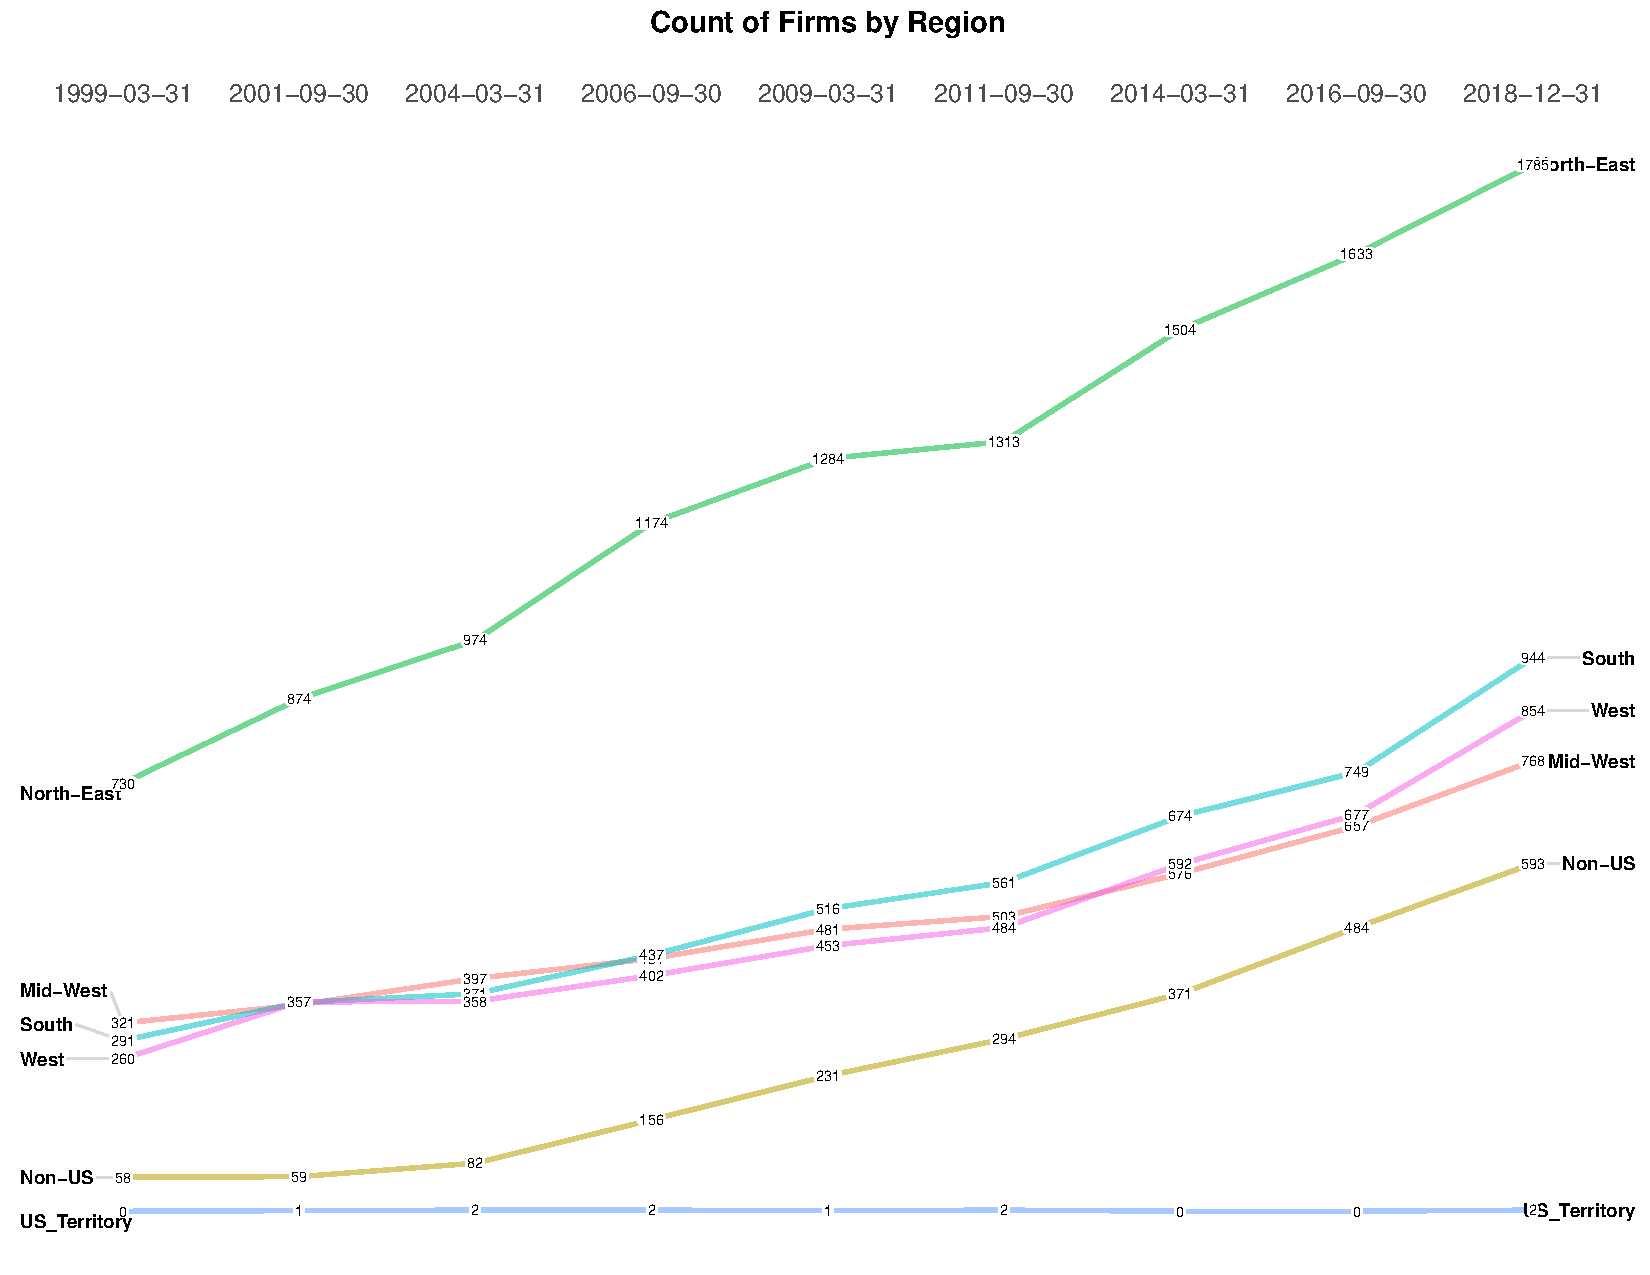
\includegraphics[width=1\linewidth]{Figures/ChapterIII/Count_firms_USA}
	\caption[Count of Institutional investors by region (as defined by the US Census Bureau) for the period 1999 to 2018]{Relative percentage of institutional investors by region during the study period (March 1999 to December 2018)}
	\label{fig:countfirmsusa}
\end{figure}

\begin{figure}
	\centering
	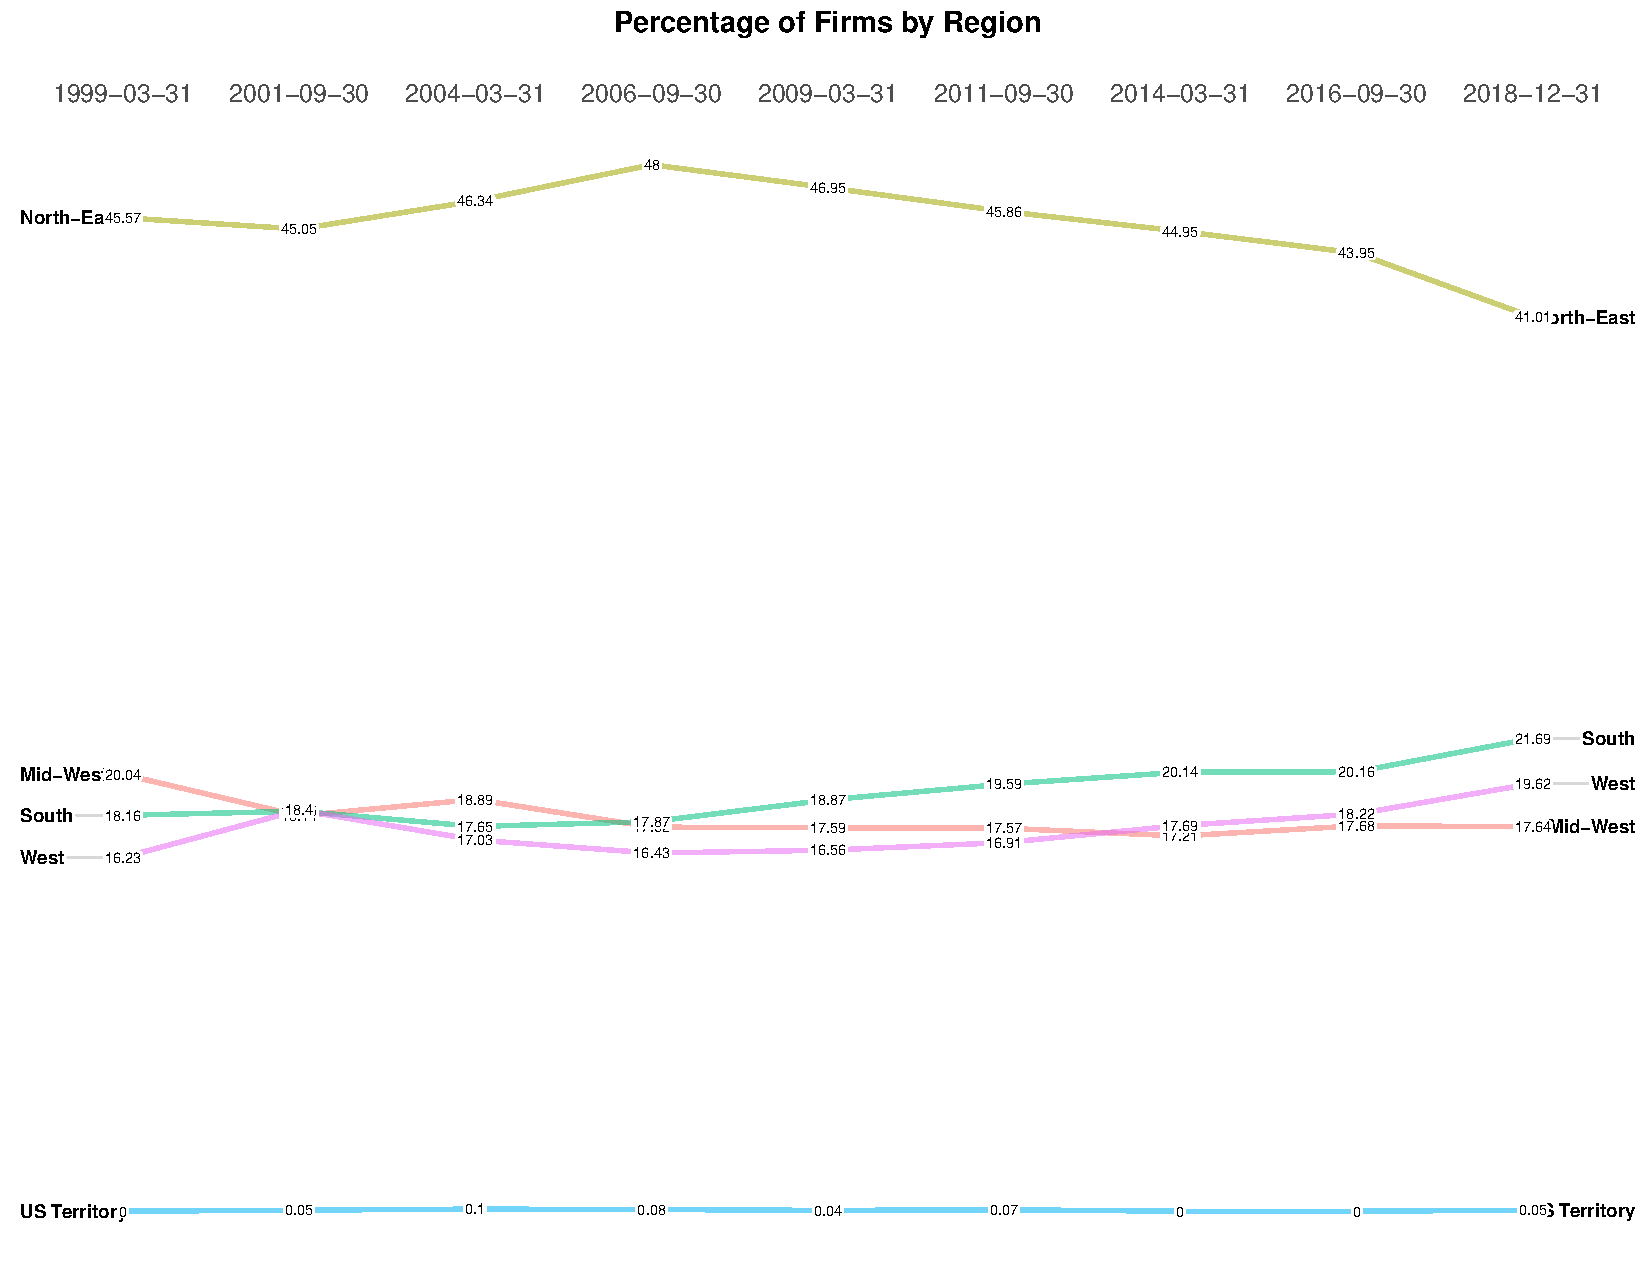
\includegraphics[width=1\linewidth]{Figures/ChapterIII/Percentage_firms_Region_USA}
	\caption{Number of Firms by Country}[Total Number of firms by region  (as defined by the US Census Bureau) during the study period (March 1999 to December 2018)]
	\label{fig:Percentage_firms_Region_USA}
\end{figure}

%\subsection{Distances}

%distances calculated with the geosphere package citep{geosphere}

\section{The K-function} 
\label{kfunction}
One of the earliest uses of point pattern analysis is the famous cholera map by Dr. John Snow.  Although he knew nothing about the cause of the bacterial outbreak, he did discover that the cases of cholera were clustered around a particular water pump on Broad Street.  Although scholarship such as \cite{brody2000map} call into question whether Dr.Snow's map was more confirmatory than exploratory since the insights into the cause of the cholera epidemic requires an understanding of germ theory.  That is to say, that Dr. Snow's maps would not be able to create their historic insights without subject matter expertise.  Regardless of whether Dr. Snow used his point density mapping technique as a starting point or only for confirmation of his hypothesis,  a common method of quantifying points in space, is measuring the intensity of the point pattern per unit of area.  Old staples used for measuring point patterns are quadrat analysis and nearest neighbour index.  However, these techniques have well known limitations such as the undue influence caused by border selection as well as the inability to determine whether points cluster or disperse at different ground scales \citep{spatstatBook}.

The examination of various ground scales is important since firms may exhibit different clustering tendencies at various scales.  The mirroring of population maps and geographic profile maps at a national scale is humorously examined in XKCD comic 1138 (Figure \ref{fig:heatmapxkcd}) \citep{XKCD1138}.  However, firms may behave differently at different scales.  For example, a national maps of firms such as coffee shops, fast food chains, banks, automated teller machines, gas stations and grocery stores may mirror the national population map, yet they would appear diffuse on a local map, for each operates their own local catchment areas.  However, other sectors such as software development have a tendency to cluster at the local and regional level \todo{Grant citation}.  

\begin{figure}
	\centering
	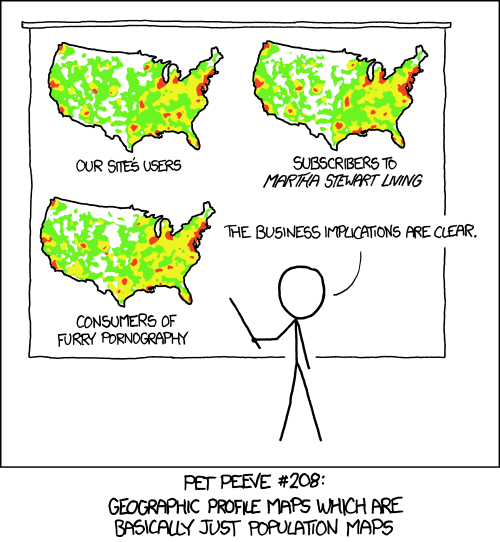
\includegraphics[width=0.7\linewidth]{Figures/ChapterIII/heatmap_XKCD}
	\caption[XKCD 1138 - Heatmaps]{XKCD \#1138 - Heatmaps by Randall Monroe. This illustrates the point that many paterns can be aproximated by human density. Used with Permission (Creative Commons Attribution-NonCommercial 2.5 License)}
	\label{fig:heatmapxkcd}
\end{figure}

At its most basic form, the K-function calculates using a Poisson process of actual vs expected counts of points within distance $h$ of each point in the data set\citep{dixon2014r}.  This yields a density function, which can be compared to the expected point pattern intensity under the conditions of complete spatial randomness at different distances.  For more information about\textit{ Ripley's K}, see \cite{ripley1976second,fischer2009handbook,spatstatBook}.

With regards to examining the clustering behaviour of institutional investors at various scales, the inherent ability to be used at various ground scales makes Ripley's K well suited for examining the clustering behaviour of institutional investors.  This facilitates the examination  of spatial clustering of institutional investors  and determines if they exhibit locational preferences closer to that of ATMs or software developers. 

The K-function in it's most basic form can be written as follows: \todo{fix this}

\begin{equation}
K(d) = \lambda^{-1}E(Nd)
\end{equation}
Where $Nd$ is the number of events $Xi$ within distance $d$ of a randomly chosen event from all points $\{X_{i},...,X_{j} \}$.  When working with a sample of data points $\{ X_{j} \}$, the K-function for the underlying distribution isn't usually known.  However, it can be estimated by using a sample.  If $d_{ij}$ 

\begin{equation}
\hat{K}(d) = \hat{\lambda}^{-1}\sum_{i}\sum_{i \neq j}\dfrac{(d_{ij} < d)}{n(n-1)}
\end{equation}

\begin{equation}
    \hat{\lambda} = \dfrac{n}{|A|}
\end{equation}

The CSR equation
\begin{equation}
    K_{csr}(d) = \pi d^{2}
    \label{eq:csr}
\end{equation}

\cite{brunsdon2015introduction}
\subsection{Spherical K-function}

The basic implementation of \textit{Ripley's K} technique assumes that the point pattern exists on a Euclidean surface.  While it may be justifiable to assume a Euclidean plain for regions of less than a few hundred kilometres \citep{HeatherJ.Lynch2008,wilschut2015spatial},  the use of Euclidean space becomes problematic above such distances, and the global distribution of institutional investors is certainly more than a few hundred kilometers, and thus spherical geometry becomes a better option. Furthermore, \cite{Tobler2002} demonstrates that while the Earth is technically an oblate spheroid, most statistical techniques on a continental scale can be done adequately on a sphere.  

The K-function displayed in Figures \ref{fig:Kfunction1}, \ref{fig:Kfunction5to100}, \ref{fig:Kfunction100to750}, and \ref{fig:Kfunction1000to5000} were performed in statistical language R using Robeson's implementation of spherical geometry \citep{SphericalK}.  This analysis was conducted with a 99-fold cross-validation, in which for each time step, the 1/99 of the data was randomly reserved from the data set\footnote{The calculation of the K function for the 80 quarters involved in this study was performed on 3 different computers for a duration of 3 months for a total of 9-computer/months calculation time}.  This creates an envelope of possible K-functions. Particular care should be noted for the third and fourth quarters of 2004.  These quarters were run a second time with a similar result, suggesting that the problem may lie with the data pipeline from Edgar rather than a sudden and reversible shift in locations preference. A similar, but less extreme discontinuity exists between the fourth quarter of 2013 and the first quarter of 2014. 

As with the other forms of measuring the concentration and dispersion at various scales seen earlier, the overall trend of initial concentration and dispersion on or after 2007 continues with the K-function.  In greater detail, Figure \ref{fig:Kfunction1} looks at the 1 km scale, where there is an initial concentration followed by a gradual diffusion starting on or around 2003. Figure \ref{fig:Kfunction5to100} shows a slightly different picture, more akin to the County and CBSA graphs of concentration from 1999 to on or about 2007 and an increased diffusion afterwards.  Figure \ref{fig:Kfunction100to750} shows a similar pattern - just not as starkly.  Finally, Figure \ref{fig:Kfunction1000to5000} shows that the continental scales resemble the shape seen in Figure \ref{fig:Kfunction1}, since there is a continual diffusion of firms from a earlier peak.  

This is an important confirmation of the trend, since Ripley's K is a point pattern analysis, and is thus immune to the  modifiable areal unit problem.  This suggests that something fundamental in the business world occurred in the time-frame of the pivot that changed the calculus in terms of benefits of the forces of agglomeration and desegregation.  There is precedence in the location preferences shifting in the past, with a substantial amount of dispersion occurring in the 1970s and 1980s when the first telecommunication revolution occurred \citep{bodenmanfirm2000}.

While it is beyond the scope of this research, it would be interesting to examine if the rise of so called business-oriented ``smartphones" by Blackberry (formerly known as Research In Motion), touchscreen smartphones such as ``iPhone" and ``Android" devices, in addition to widespread wifi-enabled cafes have reduced the productivity tax of conducting business away from the office, and thus reduce the costs of locating outside of the central business district.   

\begin{figure}[h]
	\centering
	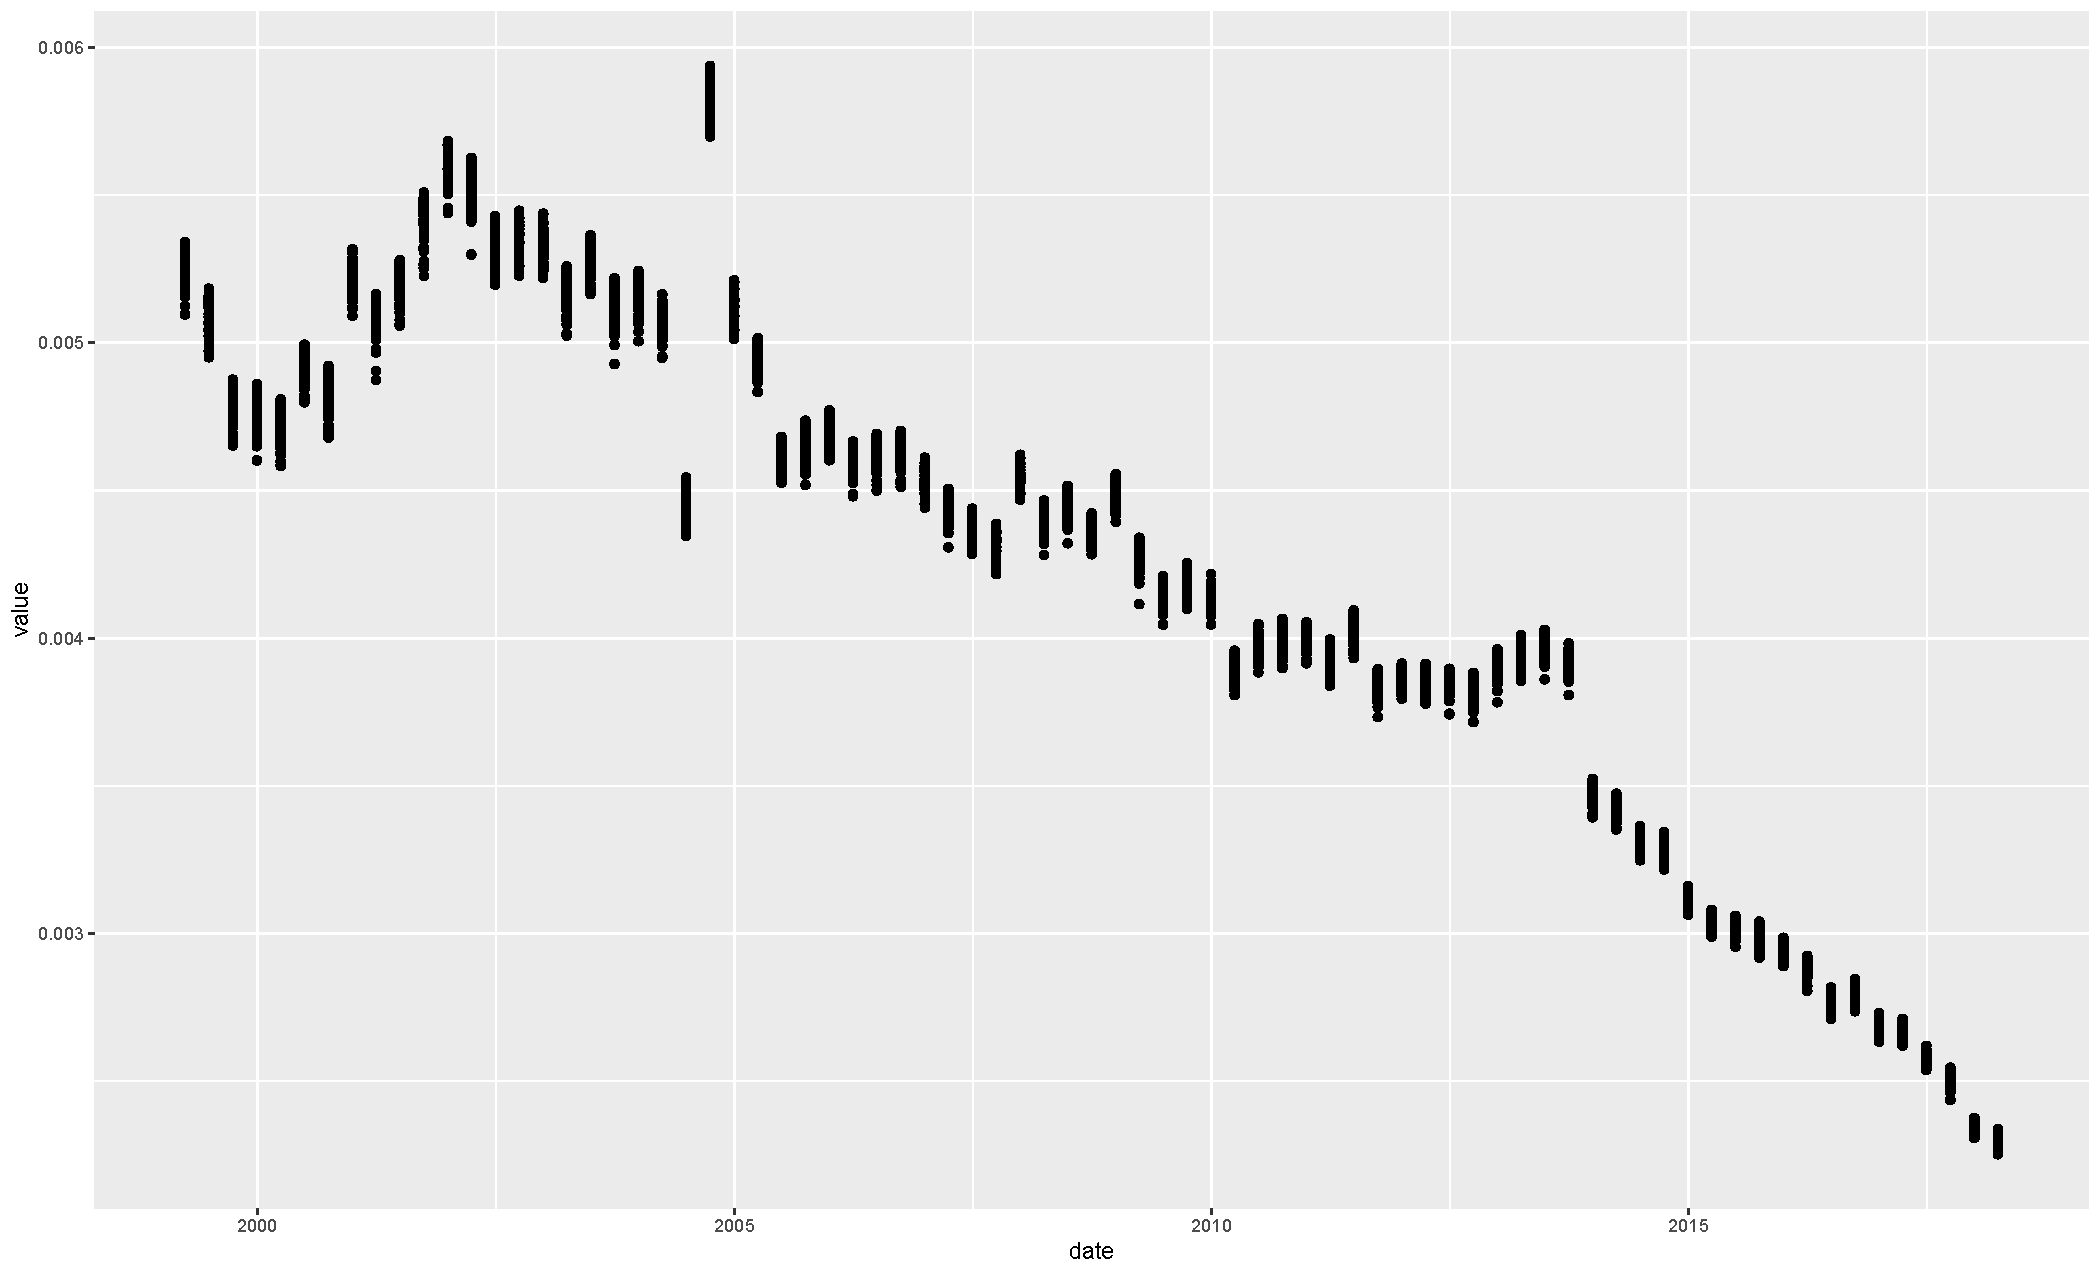
\includegraphics[width=1\textwidth]{Figures/ChapterIII/Cross_Val_1k.pdf} 
	\caption{Spherical K-function for the range band of 1 km for the years 1999 to 2018.  Each quarter consist of 99 points representing a cross-validated K-function.  }
	\label{fig:Kfunction1}
\end{figure}

\begin{figure}[h]
	\centering
	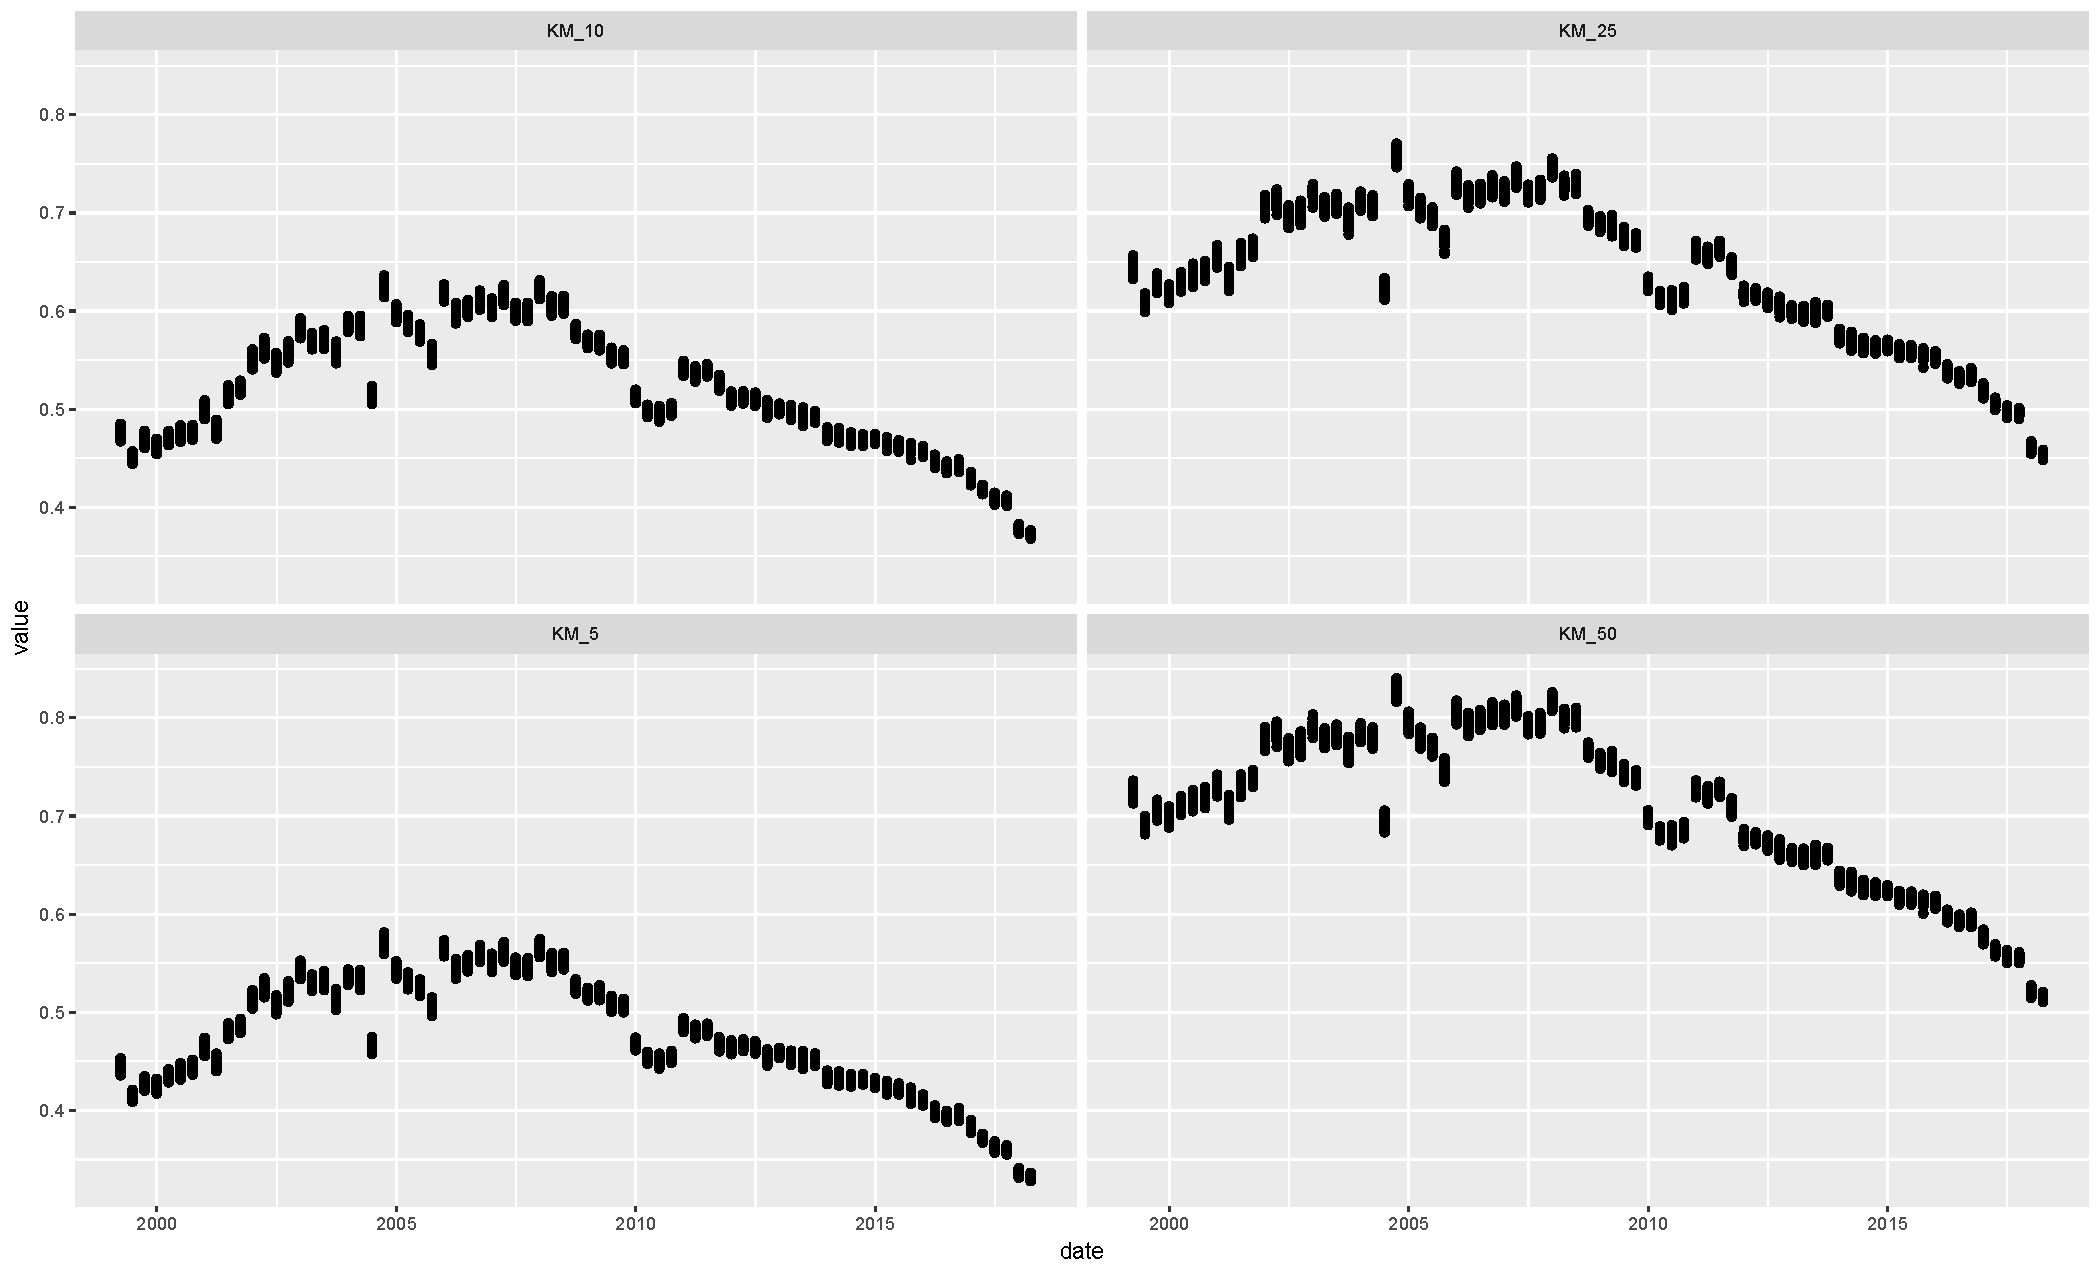
\includegraphics[width=1\textwidth]{Figures/ChapterIII/K_Function_5to50.pdf} 
	\caption{Spherical K-function for range bands 5km, 10km, 50km, 100km for the years 1999 to 2018.}
	\label{fig:Kfunction5to100}
\end{figure}

\begin{figure}[h]
	\centering
	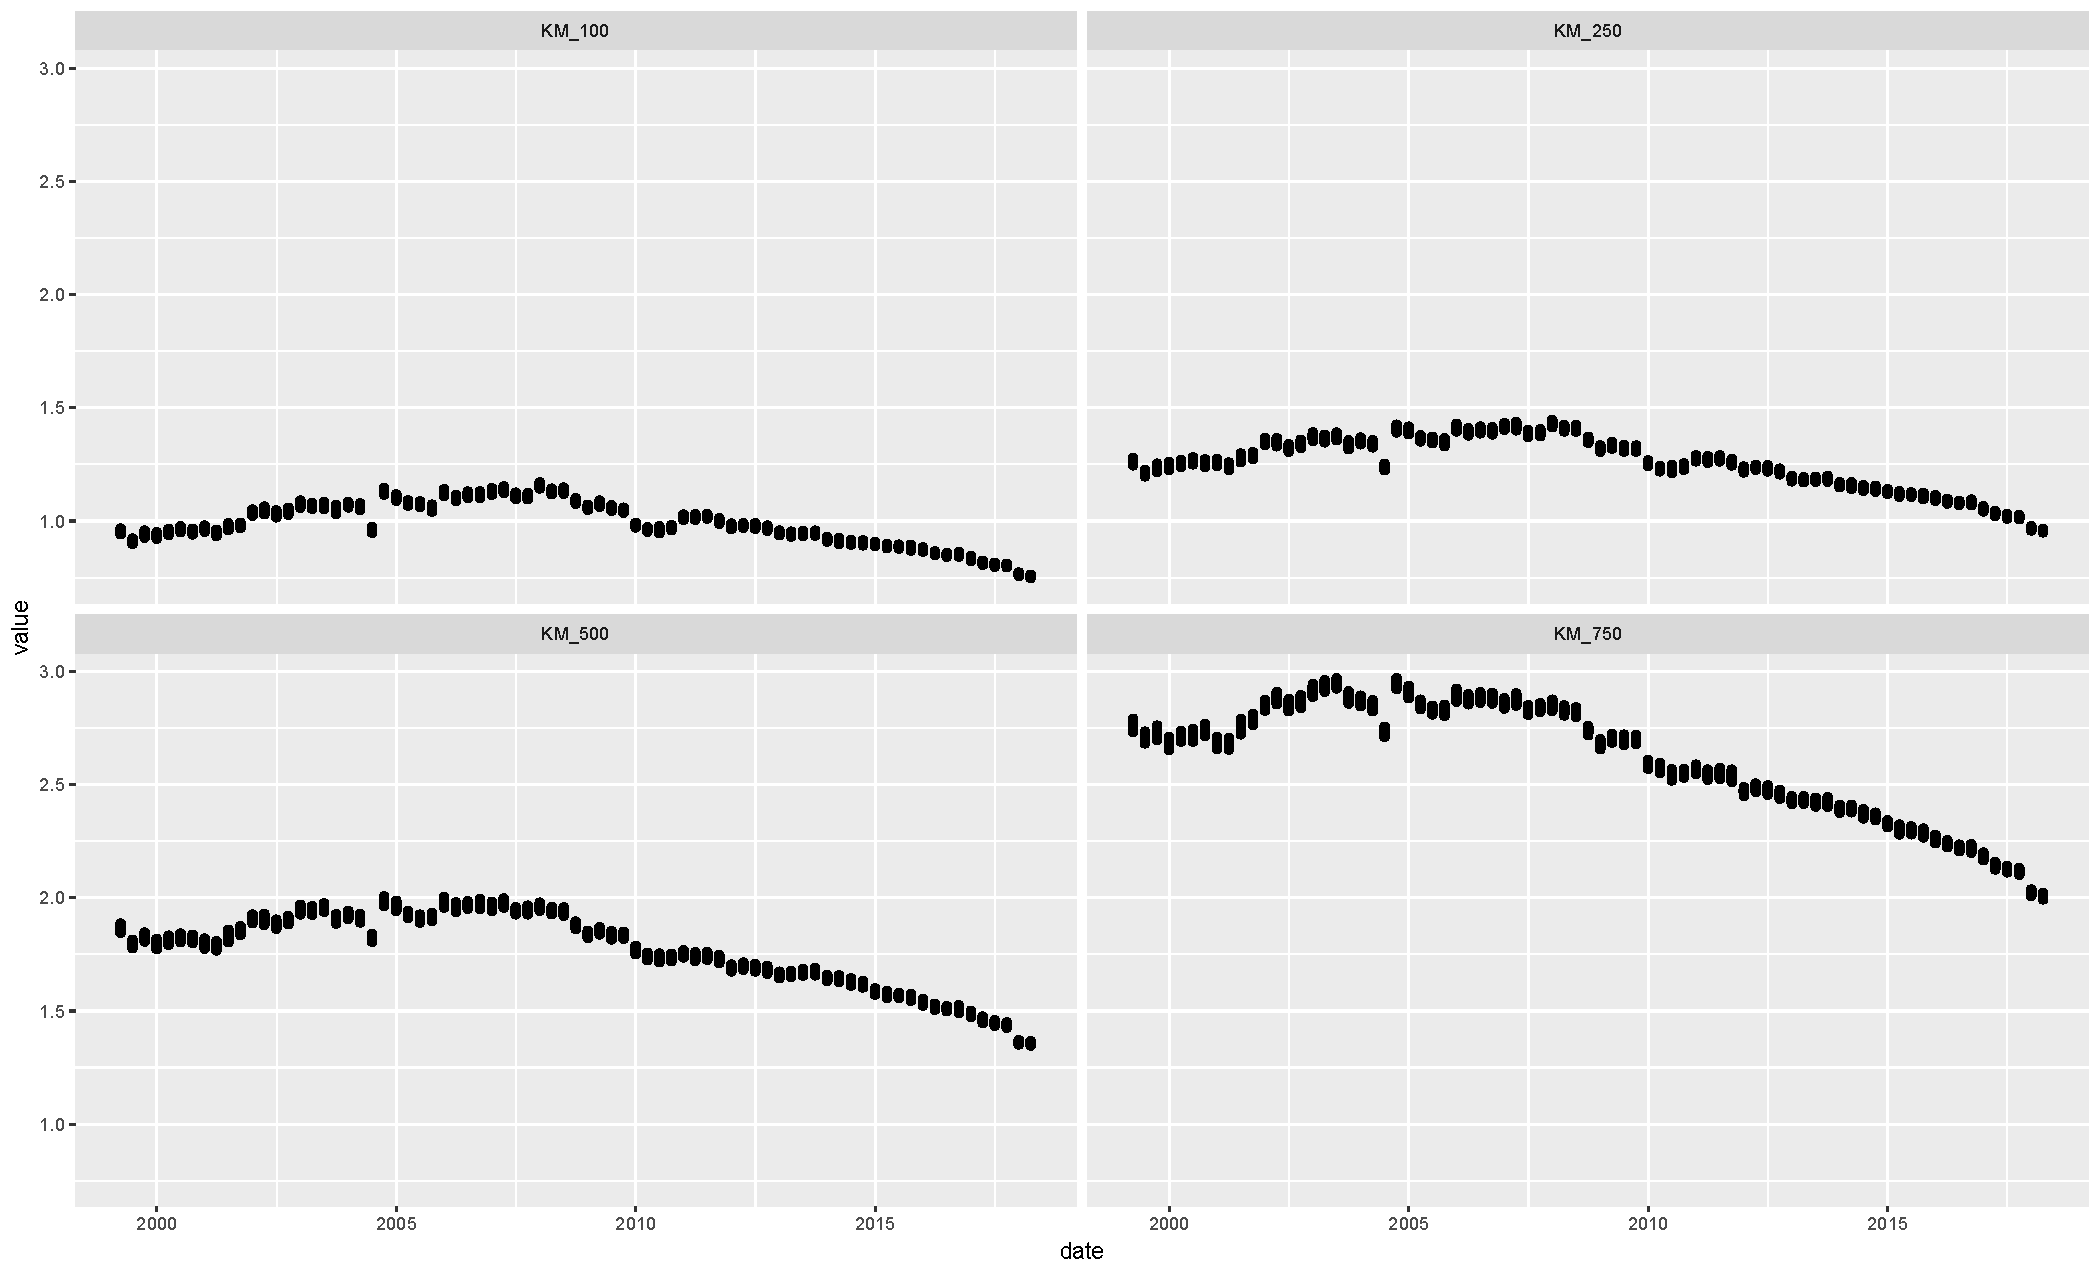
\includegraphics[width=1\textwidth]{Figures/ChapterIII/RIpley_K_100_750.pdf} 
	\caption{Spherical K-function for range bands 100 km, 250 km, 500 km, 750 km for the years 1999 to 2018.}
	\label{fig:Kfunction100to750}
\end{figure}


\begin{figure}[h]
	\centering
	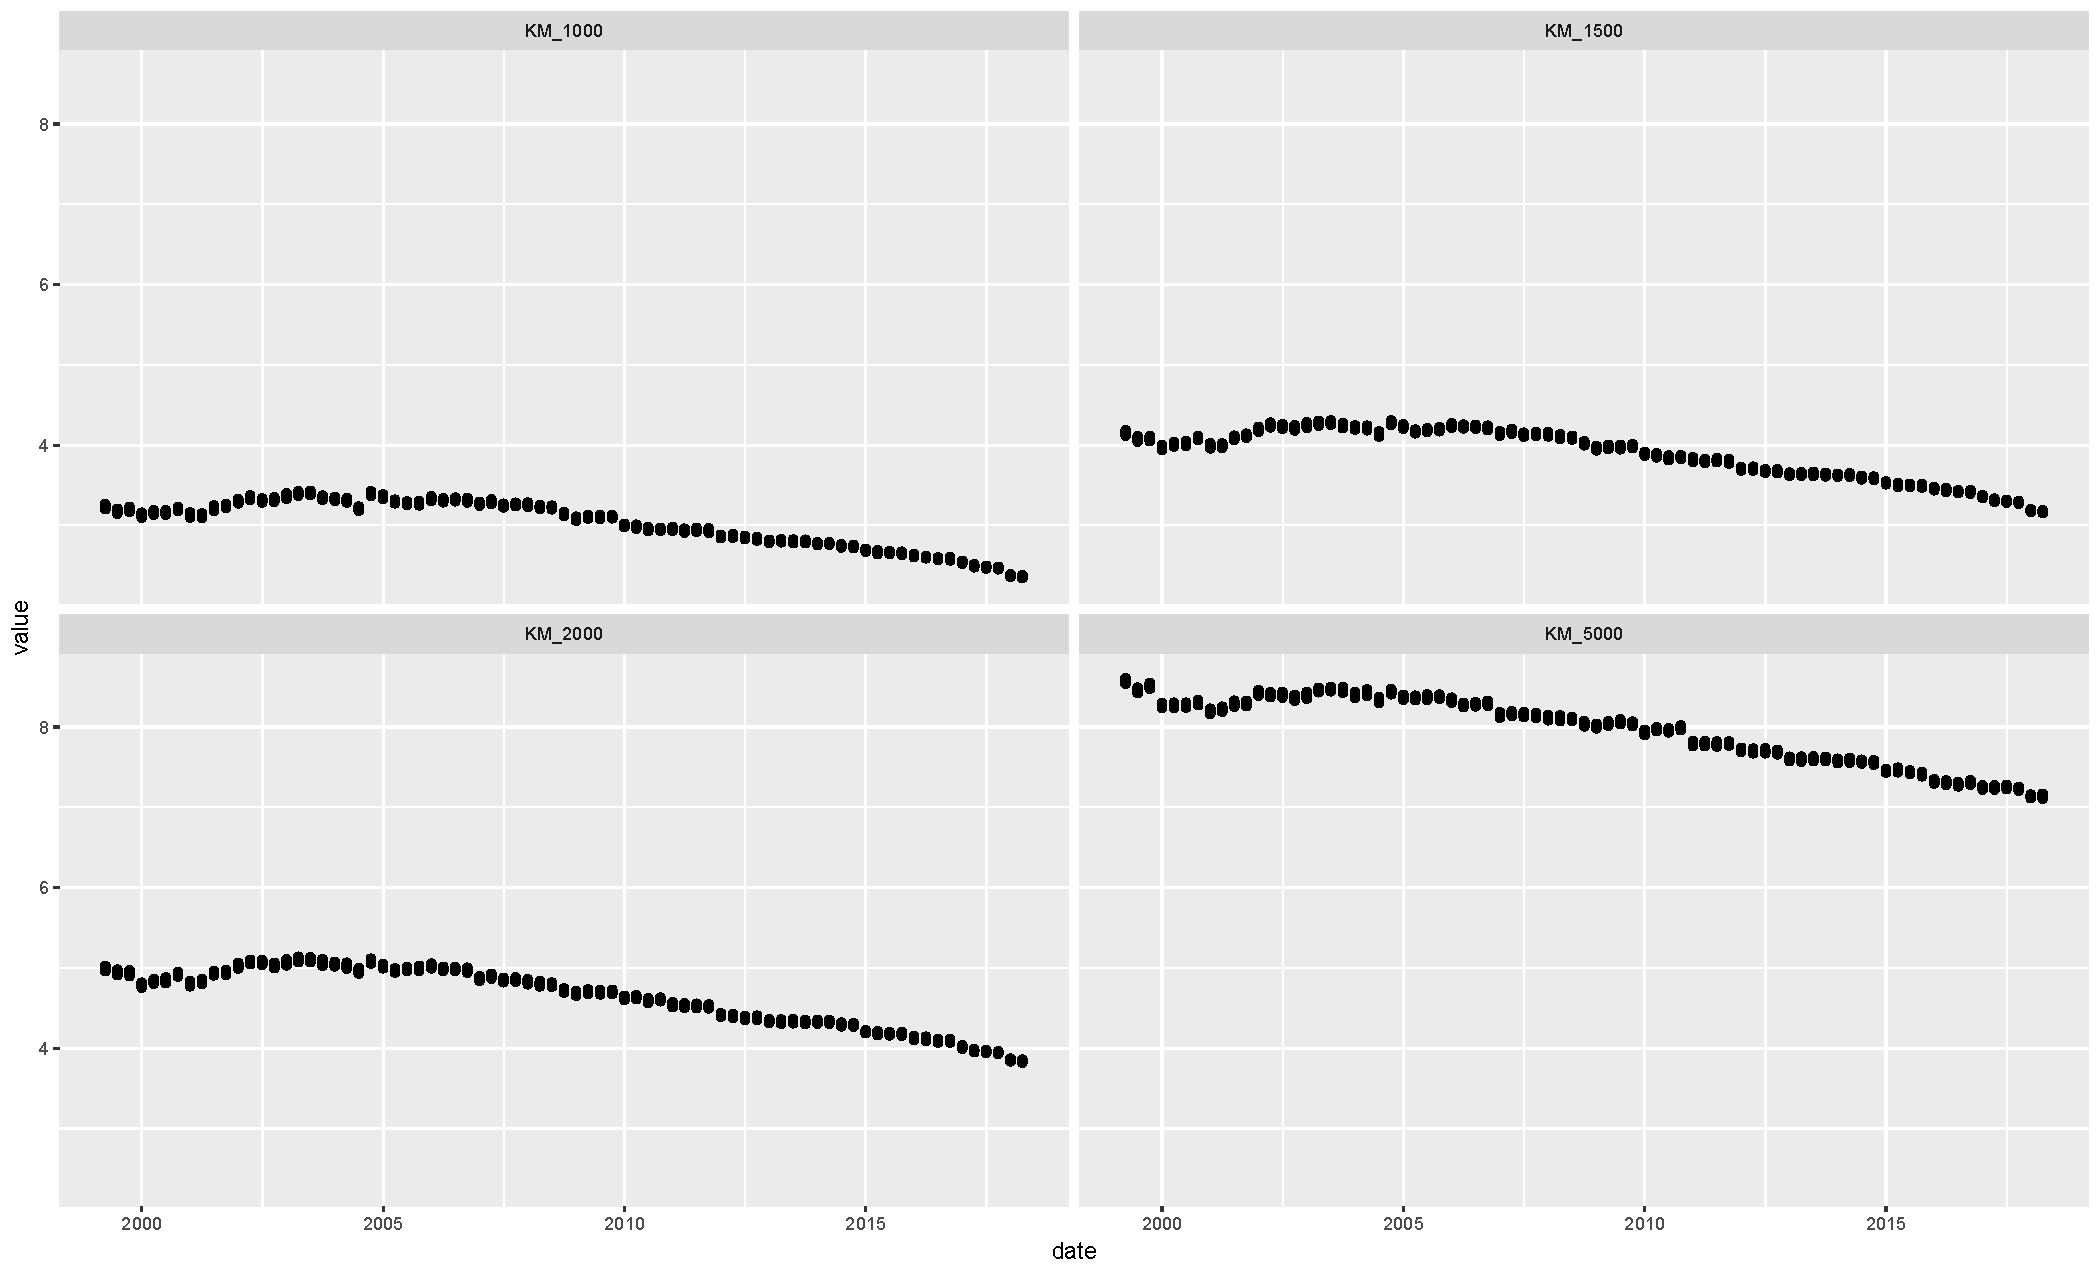
\includegraphics[width=1\textwidth]{Figures/ChapterIII/Cross_val_1000_5000.pdf} 
	\caption{Spherical K-function for range bands 1000 km, 1500 km, 2000 km, 5000 km for the years 1999 to 2018.}
	\label{fig:Kfunction1000to5000}
\end{figure}





\section{Standard Deviation Ellipsis}

The standard deviation ellipse is a useful tool in measuring the dispersion of a point pattern, and comparing the same region at different points in time in order to draw insights about a particular phenomenon \citep{Yuill1971}. The standard deviation ellipse, and its simpler cousin the standard deviation circle, create a line that enclose one standard deviation of all points from the centre of all points.  The surface area contained by this line allows researchers to characterise the concentration or diffusion of a phenomena, and multiple such ellipses allow for the examining of a trend.  Figure \ref{fig:standarddeviationellipse} shows the evolution in time of the standard deviation ellipse for the 5 cities that contain the largest amount of institutional investors. As is consistent with the other measures of clustering examined so far, these 5 cities show a long-term trend towards diffusion as investors start to show up in suburban office parks. Furthermore, while it can be somewhat imprecise to directly compare densities across cities due to the vagaries of urban planning, it is almost impossible for Los Angeles County to appear denser or more concentrated in a particular metric than New York County (Manhattan). It is immediately apparent that Los Angeles' famous urban sprawl and lack of a proper CBD create a rather diffuse concentration of institutional investors - a point that will be visited in more detail in the following chapter.  

That being said, the advantage of the standard deviation ellipse over the standard deviation circle is the addition of orientation and eccentricity. Eccentricity is measured on a scale of 0 (perfect circle) to 1 (perfect line).  An increase in eccentricity with a commensurate increase in surface area is suggestive of a new cluster being created near the perimeter of the ellipse. This is the case with regards to Boston in the mid-aughts in the Route 128 corridor (Figure \ref{fig:Standard_Deviation_ellipse_Eccentricity}). This will be examined in further detail Chapter \ref{subsection:Boston}.     

For the detailed metrics of the one standard deviation ellipse, see Appendices \ref{tab:Bos_SE} for Boston, \ref{tab:Chi_SE} for Chicago, \ref{tab:LA_SE} for Lost Angeles, \ref{tab:NY_SE} New York City and, \ref{tab:SF_SE} San Francisco.  

\begin{figure}
	\centering
	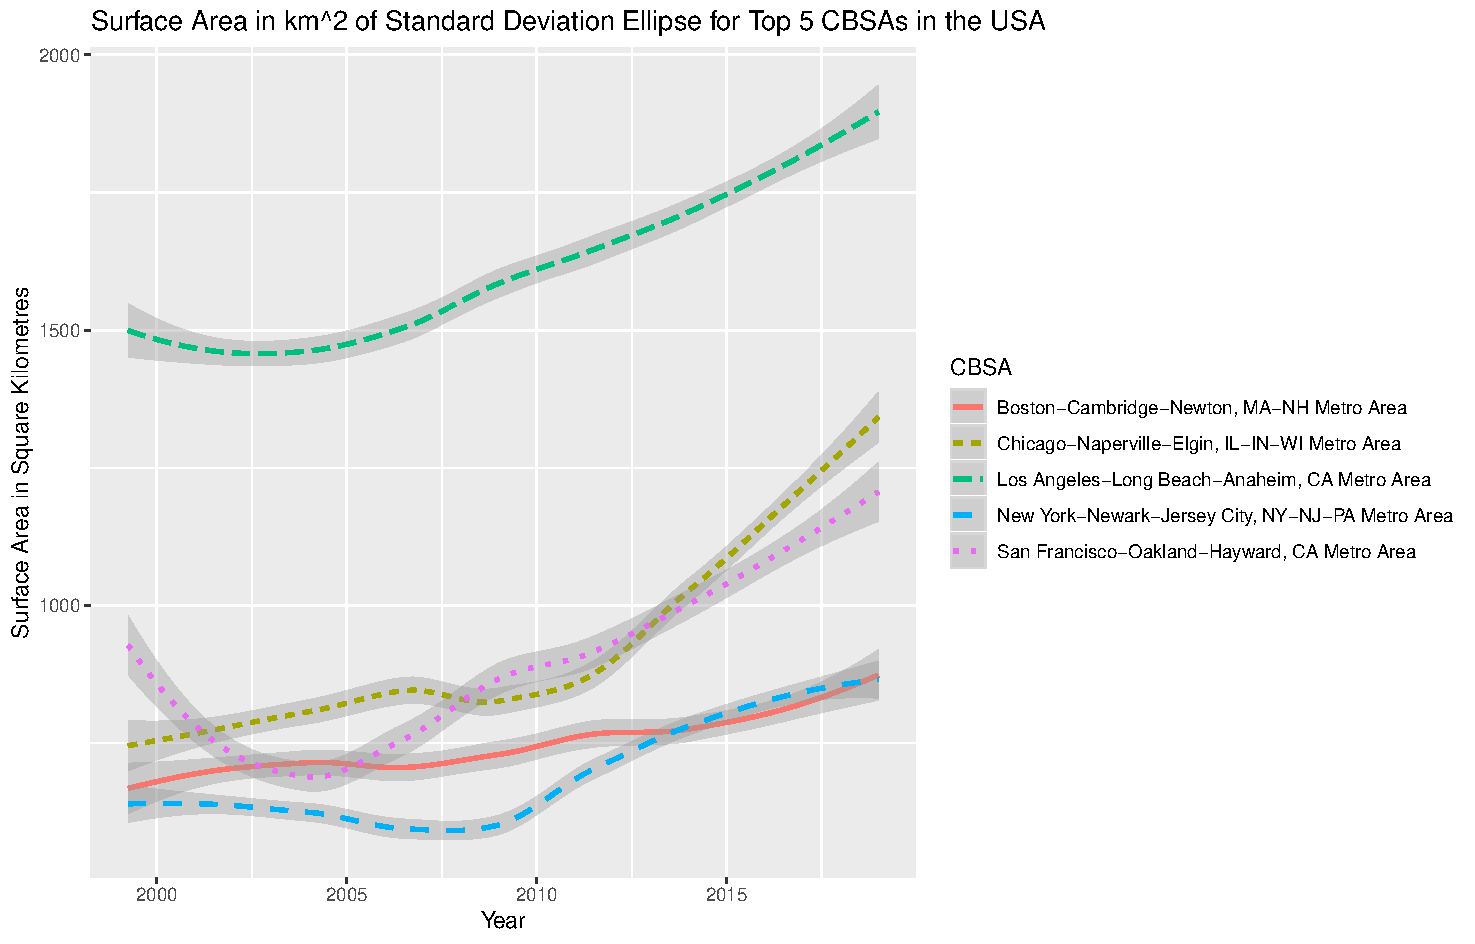
\includegraphics[width=1\linewidth]{Figures/ChapterIII/Standard_Deviation_ellipse}
	\caption[Standard Deviation Ellipse]{Standard Deviation Ellipse over time for the top 5 CBSAs by number of institutional investors for the time period of 1999 to 2018.}
	\label{fig:standarddeviationellipse}
\end{figure}

\begin{figure}
	\centering
	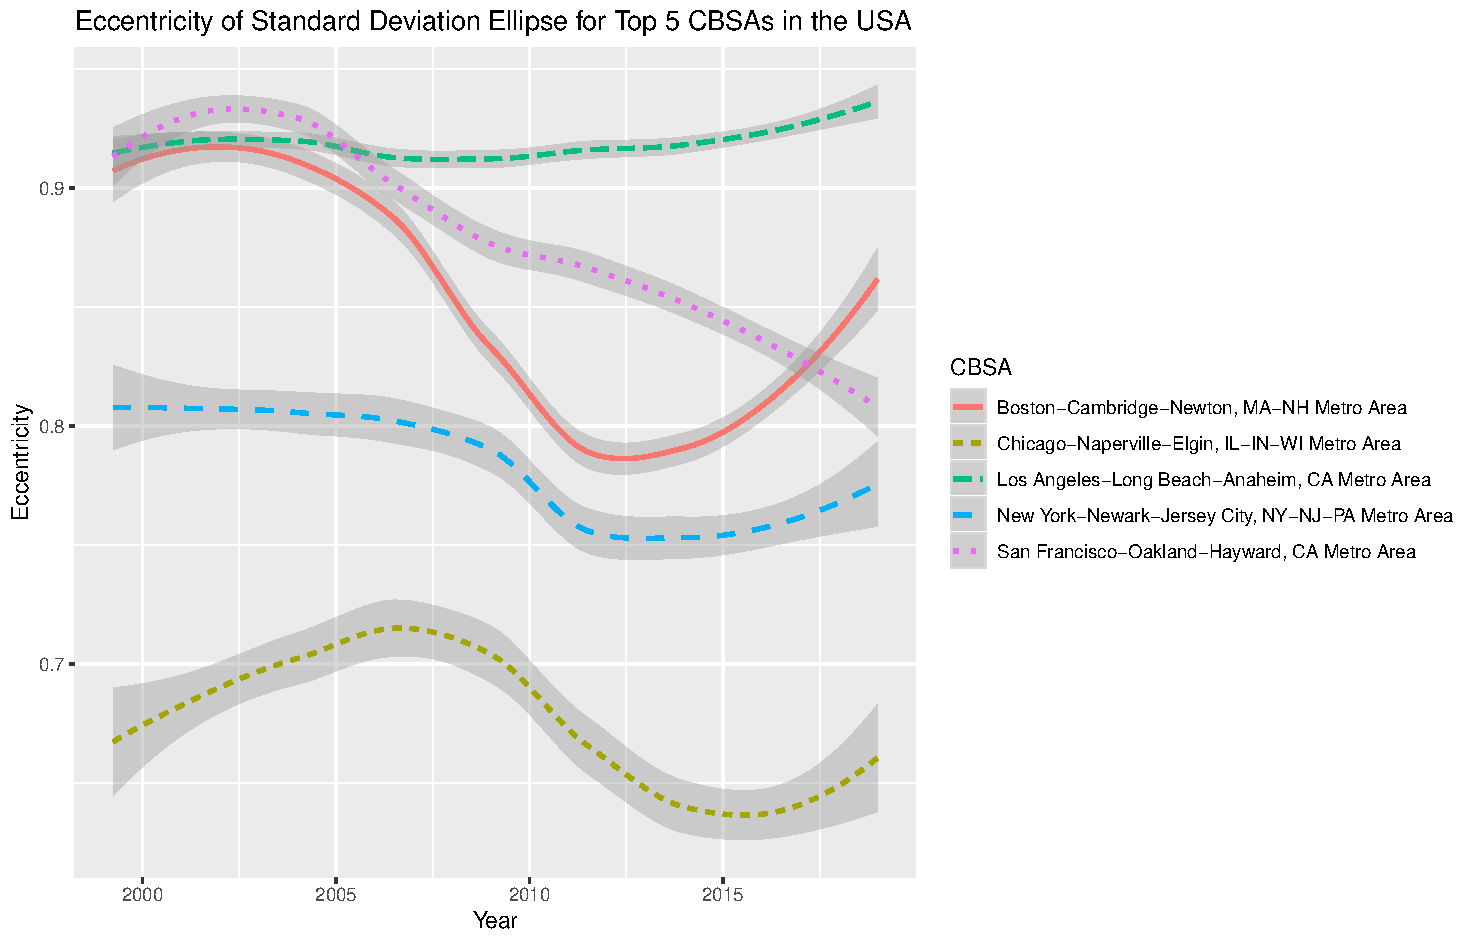
\includegraphics[width=1\linewidth]{Figures/ChapterIII/Standard_Deviation_ellipse_Eccentricity}
	\caption[Standard Deviation Ellipse Eccentricity]{Standard Deviation Ellipse Eccentricity over time for the top 5 CBSAs by number of institutional investors for the time period of 1999 to 2018.}
	\label{fig:Standard_Deviation_ellipse_Eccentricity}
\end{figure}


\section{The Gravity Model of Trade}


Gravity model of trade is an empirically derived technique to describe and predict flows from a variety of origins to destinations.  One of the first researchers to propose a model for explaining flows of population across space is  \cite{ravenstein1885laws}. He identified a series of "laws" of migration, while not explicitly referencing Newtonian gravity, identified the key variables of distance as well as push and pull factors \citep{Tobler1995}.  

The most naive way of allocating flows across a land mass is to assume a uniform distribution.  However, this is questionable at best, for this disregards a myriad of variables that can be used to account for differences in trade.  Nobody would seriously expect that trade between New York County, New York (Manhattan) and Loving County, Texas to be on the same level as that between New York County, New York and Los Angeles County, California.  Standardizing the flow by a variable such as population might help, but there's no guarantee that the flow scales solely with population \citep{Crymble19}.   

The most naive version of the gravity model is as follows:
\begin{equation}
F = G \frac{M_{1}M_{2}}{r^{2}}
\label{Naive_Gravity_Model}
\end{equation}  

Equation \ref{Naive_Gravity_Model} is inspired by Sir Issac Newton's gravity equation.  As with the gravity equation, $F$ represent the trade in goods from points $M_{1}$ to $M_{2}$. $M_{1}$ and $M_{2}$ represents the aggregate push and pull factors and is traditionally measured as the size of each's market. $r^{2}$ is the square of the distance between these points and $G$ is a constant representing the friction of trade, such as the conditions of the roads, the productivity of the longshorepeople or tariff regimes.  Unlike the theoretical apple falling from a tree (or the spherical cow thrown by a frictionless trebuchet in a vacuum), human endeavours are plagued by free will and the myriad of uncertainty that follows.  However, in an insight that could have come from Isaac Asimov's Hari Seldon, populations are easier to model than individuals, since the vagaries of human existence averages out in the aggregate.  

A gravity model's goal is to tell the user: Given a number of influencing forces (distance, costs of living, desirability, access to services, access to markets) affecting the movements of a large number of entities of the same type (fungible commodities or similarly situated people) between a set number of points, what is the most probable distribution?  Furthermore, comparing real-world flows to the model's prediction can be used to find anomalies, and these can be useful starting points for future research\citep{Crymble19}.  

With respect to the gravity model, one must make sure that the data is either complete or a representative sample of the underlying flows, else the model will be hopelessly biased.  In this case, the model will be using the universe of 13F holdings for the period of June 2013 to December 2018 to create flows between investors and to the company in which the stocks belong.  The destination information is drawn from the COMPUSAT database of stock information filings, and more specifically, the address of their headquarters which was subsequently geocoded using Google Maps \citep{Compustat}.  The push and pull factors were calculated as the total stock ownership in the 13F database for each quarter in each CBSA.  CBSAs were used for this analysis rather than States ($n=50$) or counties and their equivalents($n=3,142$) due to the CBSA's occupation of a ``sweet spot'' with regards to detail and manageability  ($n= 935$, of which there are 465 CBSAs which contain at least one flow).  

\begin{table} 
	\begin{center}
	\small
		\caption[Gravity Model of trade for Q2 2013]{Gravity model of trade as applied to investment flows between US CBSAs for the period of 2013Q2}
		\begin{tabular}{l c c c c c c }
			\hline
			& Model 1 & Model 2 & Model 3 & Model 4 & Model 5 & Model 6 \\
			\hline
			(Intercept)                  & $-7.70^{***}$ & $-7.46^{***}$ & $-6.41^{***}$ & $-29.94^{***}$ & $-6.20^{***}$ & $-29.19^{***}$ \\
			& $(0.10)$      & $(0.10)$      & $(0.10)$      & $(0.18)$       & $(0.10)$      & $(0.18)$       \\
			Distance(log)                   & $-0.09^{***}$ & $-0.13^{***}$ & $-0.23^{***}$ & $-0.31^{***}$  & $-0.26^{***}$ & $-0.33^{***}$  \\
			& $(0.01)$      & $(0.01)$      & $(0.01)$      & $(0.01)$       & $(0.01)$      & $(0.01)$       \\
			Invest. at Origin(log)                  & $0.23^{***}$  & $0.22^{***}$  & $0.18^{***}$  & $0.14^{***}$   & $0.16^{***}$  & $0.14^{***}$   \\
			& $(0.00)$      & $(0.00)$      & $(0.00)$      & $(0.00)$       & $(0.00)$      & $(0.00)$       \\
			Invest. at Destination(log)                 & $0.20^{***}$  & $0.20^{***}$  & $0.15^{***}$  & $0.12^{***}$   & $0.15^{***}$  & $0.12^{***}$   \\
			& $(0.00)$      & $(0.00)$      & $(0.00)$      & $(0.00)$       & $(0.00)$      & $(0.00)$       \\
			Origin Is State Capital          &               & $1.86^{***}$  &               &                & $1.82^{***}$  & $1.45^{***}$   \\
			&               & $(0.04)$      &               &                & $(0.04)$      & $(0.04)$       \\
			Dest. is State Capital     &               & $0.93^{***}$  &               &                & $0.70^{***}$  & $0.18^{***}$   \\
			&               & $(0.04)$      &               &                & $(0.03)$      & $(0.04)$       \\
			Origin Population           &               &               & $0.00^{***}$  &                & $0.00^{***}$  &                \\
			&               &               & $(0.00)$      &                & $(0.00)$      &                \\
			Destination Population      &               &               & $0.00^{***}$  &                & $0.00^{***}$  &                \\
			&               &               & $(0.00)$      &                & $(0.00)$      &                \\
			Origin Population(log)      &               &               &               & $2.50^{***}$   &               & $2.38^{***}$   \\
			&               &               &               & $(0.02)$       &               & $(0.02)$       \\
			Destination Population(log) &               &               &               & $2.40^{***}$   &               & $2.38^{***}$   \\
			&               &               &               & $(0.02)$       &               & $(0.02)$       \\
			\hline
			R$^2$                        & 0.24          & 0.25          & 0.33          & 0.31           & 0.34          & 0.31           \\
			Adj. R$^2$                   & 0.24          & 0.25          & 0.33          & 0.31           & 0.34          & 0.31           \\
			Num. obs.                    & 214832        & 214832        & 214832        & 214832         & 214832        & 214832         \\
			RMSE                         & 5.17          & 5.14          & 4.85          & 4.93           & 4.82          & 4.91           \\
			\hline
			\multicolumn{7}{l}{\scriptsize{$^{***}p<0.001$, $^{**}p<0.01$, $^*p<0.05$}}
		\end{tabular}
		
		\label{table:coefficients_gravity_2013Q2}
	\end{center}
\end{table}

The resultant flows matrix was quite porous, with X of Y cells being otherwise empty.  This poses a problem for the model, since zero is undefined when transformed by logarithm.  A quick and dirty remedy for this is to add a dummy transaction of 1/10 000 of USD to each CBSA.  For each cell that would otherwise reported zero flow now reports 0.005 USD in flows.  While the value of 0.005 USD is too small to be represented in hard currency, this value will give a defined value when transformed.  

\subsection{Discussion}

In total, 6 models were run for each quarter for a total of 114 total models.  Since there is very little quarter to quarter variation between model runs, only the model for the second quarter of 2013 (June 30th, 2013) will be discussed here.  The results of the other quarters are available in Appendix \ref{GravityModelappendix}.  

The first model is the most naive model possible where only the distance between CBSAs, as measured CBSA centroid to CBSA centroid, as well as the investment capital available in each origin and destination are considered.  Consistent with previous literature such as \cite{Green1995,gravesthe1998,covalhome1999,covalthe2001,Dovak2005}, model 1 (Table \ref{table:coefficients_gravity_2013Q2}) shows a significant distance decay function in the flows between different CBSAs. Furthermore, this naive model can explain 24 percent of the variance seen in the network of flows.  

Examining the residuals of the naive model, the largest outliers are where the model drastically underestimated the flows between large cities with robust financial centres, such as Boston to New York, San-Francisco to New York, New York to San-Francisco, New York to Boston. At the other side of the outliers the model has trouble factoring eccentric portfolio choices, such as foundations being bequeathed large amounts of a single stock.  One such notable example is the Kellogg W. K. Foundation Trust, for it is a holder of a large amount of Kellogg stock located in the relatively rural city of Battle Creek Michigan, the historical home of the Kellogg Corporation, yet shows no ties to nearby large financial centres such as Chicago or New York, as well as mid to lower tier financial centres such as Detroit or Minneapolis-Saint Paul.  

Models 2 through 4 build on the naive model by adding an extra explanatory variable.  In the case of model 2, binary variables were added to the model representing if the CBSA contained a State capital.  This was added in order to control for the observation that many State pension funds are located in their Capitol city (at least from an administrative capacity) rather than in a nearby financial centre, such as the various New York State employees and teachers pension funds being controlled out of Albany NY rather than New York City.  Similarly, one can point to the California Public Employees' Retirement System  (CalPERS) and the California State Teachers' Retirement System (CalSTRS) being run out of Sacramento California rather than San Francisco or Los Angeles.  Unsurprisingly, model 2 shows this to be a significant factor in predicting monetary flows. This is consistent with the literature such as \cite{Bradley2016} that examines the role of State-level power brokers in fostering a suitable business environment.

Model 3 adds the human population of the CBSA as a variable, while model 4 adds this population transformed by the logarithm of the population.  Here the untransformed population count is a better predictor variable of flows than the log of the population when looking at the adjusted $r^{2}$ and Root Mean Square Error (RMSE).  \nomenclature{RMSE}{Root Mean Square Error}

Models 5 and 6 are kitchen sink approaches, where all of the explored explanatory variables are included in the model.  It should be noted that the human population of the origins and destinations are not examined at the same time as the log of human population since this would be in effect measuring the same thing twice, and thus unbalancing the model by adding covariates.  

Taken as an ensemble, Model 5 has the lowest residual mean square error and hightest $r^{2}$.  This model suggests that there is definitely is a distance decay function with regards to investing.   

\section{Conclusion}

This chapter performs an exploratory treatment of the data from various geographic scales and using simple geographic techniques.  Across the different scales of analysis (state, CBSA, county, and point), and technique from simple counts to more computer intensive techniques such as the K-function and standard ellipse, there is a broad agreement that overtime the locational preferences of investors steer toward slightly less concentration, while still maintaining a decidedly major metro area preference.  This time period shows a continued relative decline of New York City within the American hierarchy of financial cities.  However, it is important to note that this decline is only relative, and that New York City is still the number one location for new institutional investors in the absolute sense.  

Lastly, the gravity model of trade as applied to institutional investors suggests that distance plays a part in investment flows, and that distance decay can be measured.  Furthermore, the less naive models continue to show the importance of State Capitals and large metro areas with regards to locating institutional investors, suggesting that institutional investment continues to play a strong command and control function within the American and world economy. 
		\chapter{Space Time}	
\label{chapterIV}
\section{Introduction}

The previous chapter shows that institutional investment is mostly an urban phenomenon.  This chapter examines the evolution of institutional investors across space and time.  Furthermore, for ease of statistical analysis, both databases will only draw from investors located in the continental United States (CONUS), as well as for the top 5 core-based statistical areas (CBSA) in terms of total institutional investment.  In alphabetical order, these 5 metro regions are Boston, Chicago, Los Angeles, New York City and San Francisco.  


\section{Space-Time Cube}

The space-time cube is a space-time analytical technique that bins point objects into a space-time grid in order to examine the relationship between points not only in space, but across time \cite{Esri}. Two types of space-time cubes are created, the first one aggregates the total number of institutional investors for the time period of March 1999 to December 2018.  The second space-time cube aggregates the total number of funds under management for the period of June 2013 to December 2018.  

The first step in creating a space-time cube is the creation of a Network Common Data Form (NetCDF) file.   This file format permits ArcGIS to store multidimensional information with a defined geographical position (x and y) alongside a defined time period as well as any additional relevant information such as count data, sum, average, median and standard deviation.  This creates a data-structure in which further analysis can be performed, such as emerging hotspot analysis and local outlier analysis. Figure \ref{fig:timecube1} provides two perspectives on the data aggregation process. 

\begin{figure}
	\centering
	
	
	\begin{subfigure}[b]{0.45\textwidth}
		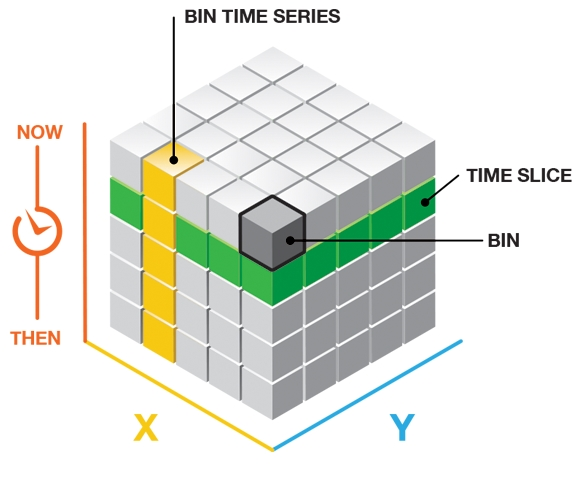
\includegraphics[width=1\linewidth]{Figures/ChapterIV/TimeCube}
		\caption{A schematic explanation of the timecube }
		\label{fig:Timecube}
	\end{subfigure}
	\begin{subfigure}[b]{0.45\textwidth}
		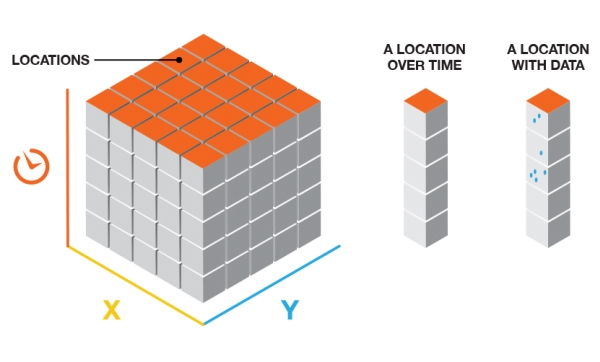
\includegraphics[width=1\linewidth]{Figures/ChapterIV/Time_Cube_Slice}
		\caption{Examination of a timecube cell}
		\label{fig:timesclice}
	\end{subfigure}
	
	\caption[ESRI Schematic Illustrations of a TimeCube]{Schematic Illustration of a TimeCube. It should be noted that unlike this schematic representation of the time cube, the analysis in this paper uses a hexagonal bin rather than a square bin for spatial data.  Image from: \url{http://desktop.arcgis.com/en/arcmap/10.3/tools/space-time-pattern-mining-toolbox/visualizing-cube-data.htm}}
	\label{fig:timecube1}
\end{figure}


It should be noted that unlike Figure \ref{fig:Timecube} and \ref{fig:timesclice}, this analysis was run using hexagonal bins. Unlike the traditional square bins (or in Esri's parlance, a fishnet grid), the hexagons have multiple advantages over squares, such as:  of the three geometric forms that can tessellate (repeat a shape over and over without overlap), the  square, the hexagon and the equilateral triangle, hexagons have the lowest perimeter to area ratio.  This is due to hexagons being the closest of the three tessellating shapes to a circle.  As such, this reduces the border effect when binning points, since the hexagon has the shortest average distance between perimeter and centroid.  Furthermore, the centroids of hexagons are equidistant from each other when tessellated.  This cannot be said about squares in a grid using the queen's movement, for the distances between centroids in square bins are shorter along the rook's movement than the bishop's movement due the the Pythagorean theorem.  Lastly, at larger distances hexagons suffer less distortion than squares.  Unfortunately for square bins, the implementation of spatial bins in this project does not play to its strengths, such as ease of use when conducting matrix algebra and having an orthogonal coordinate system \citep{birch2007rectangular}. 

With regards to the time dimension of the data, the dates are aligned such that bins coincide with the last date in the datasets (December 31, 2018), and work backwards from there in 3 month intervals.  As such, each temporal bin covers one filing period for 13F-HR disclosures.  (Figure \ref{fig:timesclice})

\subsection{Emerging Hot Spot Analysis}

Emerging hot spot analysis is the space-time implementation of the Getis-Ord Gi* statistic \citep{getis2010analysis}, and examines whether high or low values cluster geographically.  High $g$ values are created when the local sum and that of its neighbours are significantly larger than their proportion to the global sum, with low values in the reverse case. The ArcGIS implementation of Emerging Hot Spot Analysis performs the False Discovery Rate (FDR) correction.  FDR accounts for multiple testing, and therefore compensates for the possibility that certain features would be classified as hot or cold by chance alone \citep{Esri}.

The next step is to perform Mann-Kendall trend test to detect temporal trends at each spatial location. Depending on the results of the Getis-Ord Gi* statistic and the trend direction from the Mann-Kendall test, there is a total of 17 possible answers, and their definitions are listed in Table \ref{App:EmergingHotspotdef} in Appendix \ref{Definition_appendix} \citep{Esri}.

\subsection{Local Outlier Analysis}

Local outlier analysis is the space-time implementation of the Anselin Local Moran's I statistic.  This tool identifies concentrations of high values (high-high), low values (low-low) in addition to spatial ouliers in which high values are surrounded by low values (high-low), and low values that are surrounded by high values (low-high).  Unlike traditional Anselin Local Moran's I statistic, the local outlier analysis variant offers a 5th category, in which it flags bins that have different Anselin Local Moran's I statistic values during the timeframe.  

\section{United States of America}

The first use of space-time analysis will focus on the United States as a whole, after which the basic analysis will be repeated on the five largest metro areas. 

When creating the NetCDF file for the United States of America, the size of spatial bins was set at 50 km.  This value was chosen since this permitted a local window with a radius of 300 km according to the ESRI implementations of Emerging Hotspot Analysis and Local Outlier Analysis.  This latter figure is important since it would represent the longest possible day trip during a business day \citep{Fritsch06}.  Furthermore, we should keep in mind that the 50 km range band showed one of the highest level of change over time with regards to the K-function.  

\subsection{Count Data}

Figure \ref{fig:usahspcount} shows the results of the emerging hotspot analysis using the address book database. These results should come as no surprise after reading the previous chapter, in which the vast majority of institutional investors are located in the New York, Boston, Chicago, Los Angeles and San Francisco regions.  After all, institutional investment is a decidedly urban phenomenon despite being a theoretically footloose industry in an era of wireless telecommunications and computerized stock trading.  In addition to these regions, there is some strong, but inconsistent growth in the Texas Triangle (a megaregion that encompasses San Antonio, Dallas-Fort Worth and Houston), the Miami-Dade region of South Florida, the Ohio Valley and the Raleigh Triangle (Raleigh, Durham and Chapel Hill, North Carolina).  


\begin{figure}[h]
	\centering
	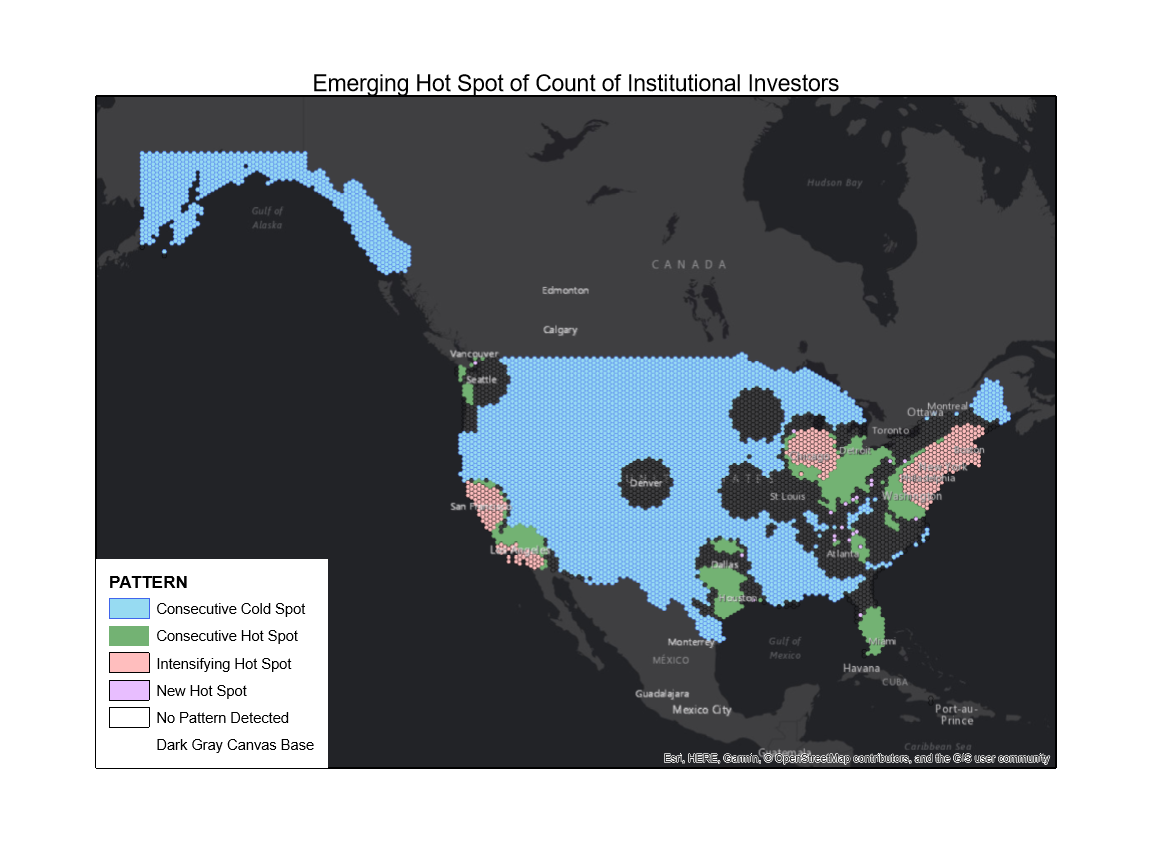
\includegraphics[width=1\linewidth]{Figures/ChapterIV/USA_HSP_Count}
	\caption[Emerging Hot Spot Analysis of Locations of Institutional Investors in the USA]{Emerging Hot Spot Analysis of locations of Institutional Investors in the United States of America for the period of March 1999 to December 2018.}
	\label{fig:usahspcount}
\end{figure}

Painting a similar picture than Figure \ref{fig:usahspcount},  the local outlier analysis (Figure \ref{fig:usaloacount}) indicates that the cities of New York, Boston, Chicago, Los Angeles and San Francisco are high-high clusters.  

What is also of interest, is the light sprinkling of high-low clusters in Figure \ref{fig:usaloacount}.  These light blue dots coincide with secondary and tertiary financial centres as well as State capitals where State-employee pension funds are managed.  
Low-high clusters appear to be confined to bridging the gaps between nearby high-high clusters, such as the peripheral areas of the North-East mega-region.  These low-high clusters are not unexpected, since they are definitionally low areas surrounded on multiple sides by high areas.     

\begin{figure}
	\centering
	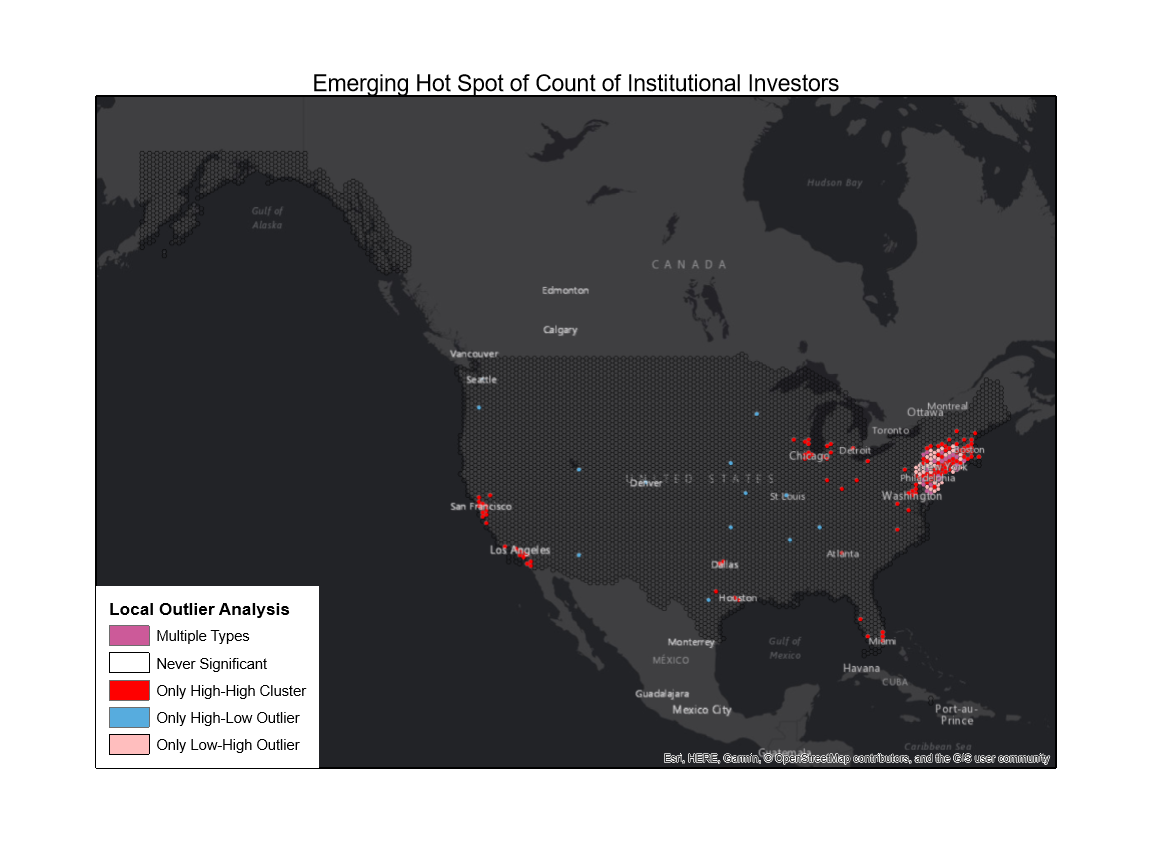
\includegraphics[width=1\linewidth]{Figures/ChapterIV/USA_LOA_Count}
	\caption[Local Outlier Analysis for Number of Institutional Investors in the USA]{Local Outlier Analysis for Number of Institutional Investors in the USA for the time period March 1999 to December 2018}
	\label{fig:usaloacount}
\end{figure}

\subsection{Funds under Management}

Using the same technique on the holdings database presents a slightly different  outcome as seen in Figure \ref{fig:usaHSP_Money}. Using money under management rather than count data puts more emphasis on New York and San Francisco, while at the same time removing all of the consecutive cold spot areas and turning them into regions with no detectable patterns.  	

\begin{figure}
	\centering
	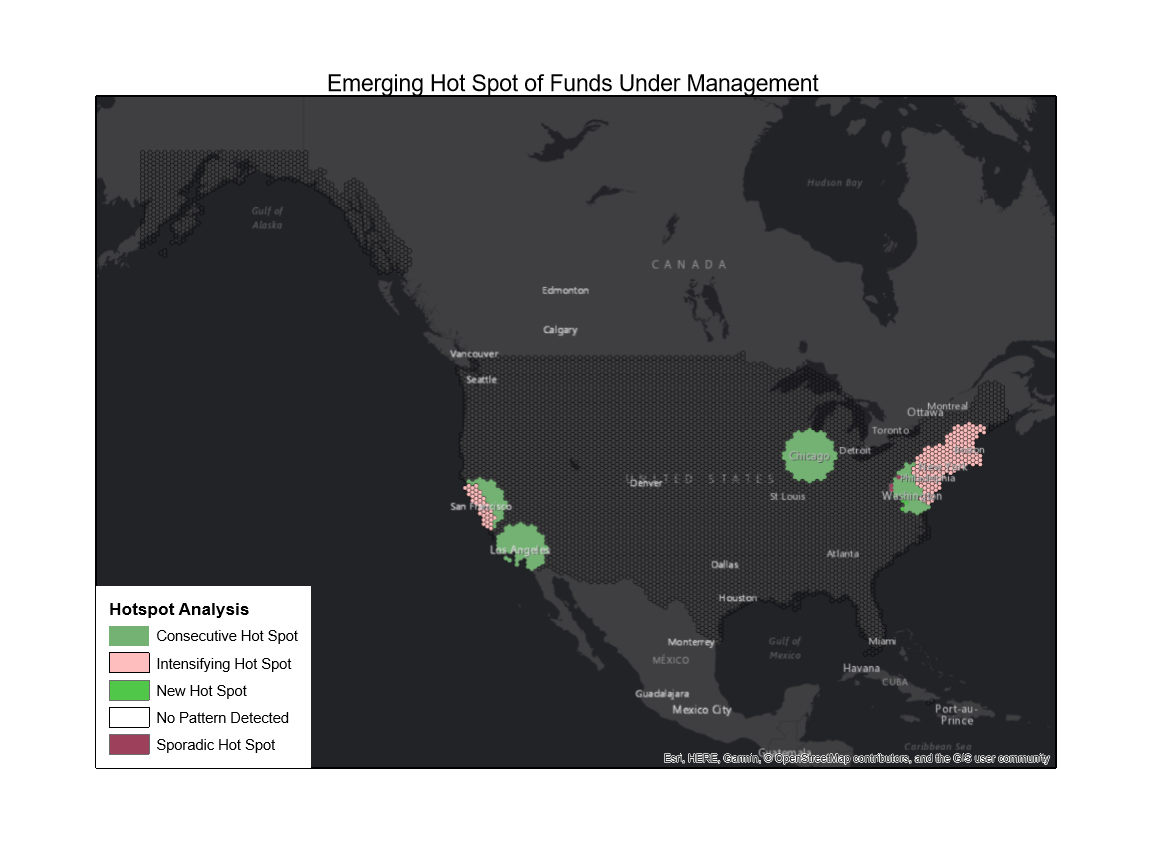
\includegraphics[width=1\linewidth]{Figures/ChapterIV/USA_HSP_Money}
	\caption[Local Outlier Analysis of USA-based Institutional Investors]{Local Outlier Analysis of USA-based Institutional Investors located in the United States of America for the period of March 1999 to December 2018. }
	\label{fig:usaHSP_Money}
\end{figure}	


As with Figure \ref{fig:usaHSP_Money}, which is based on the holdings database, the local outlier analysis (Figure \ref{fig:usaloamoney}) is much more restrained than the analysis done on the address book database.  Immediately noticeable is the absence of the high-low hexes dotting the capitals of fly-over states, as well as the more restrained presence of low-high clusters in the Bos-NY-Wash.  Lastly, as a lone bright spot in a sea of nothingness, Atlanta is the only place outside of the 5 largest US cities for institutional investment that is a high-high hex.  This is consistent with the trend seen in Chapter \ref{Atlanta} where Atlanta was becoming the financial centre of the US South-East. 

\begin{figure}
	\centering
	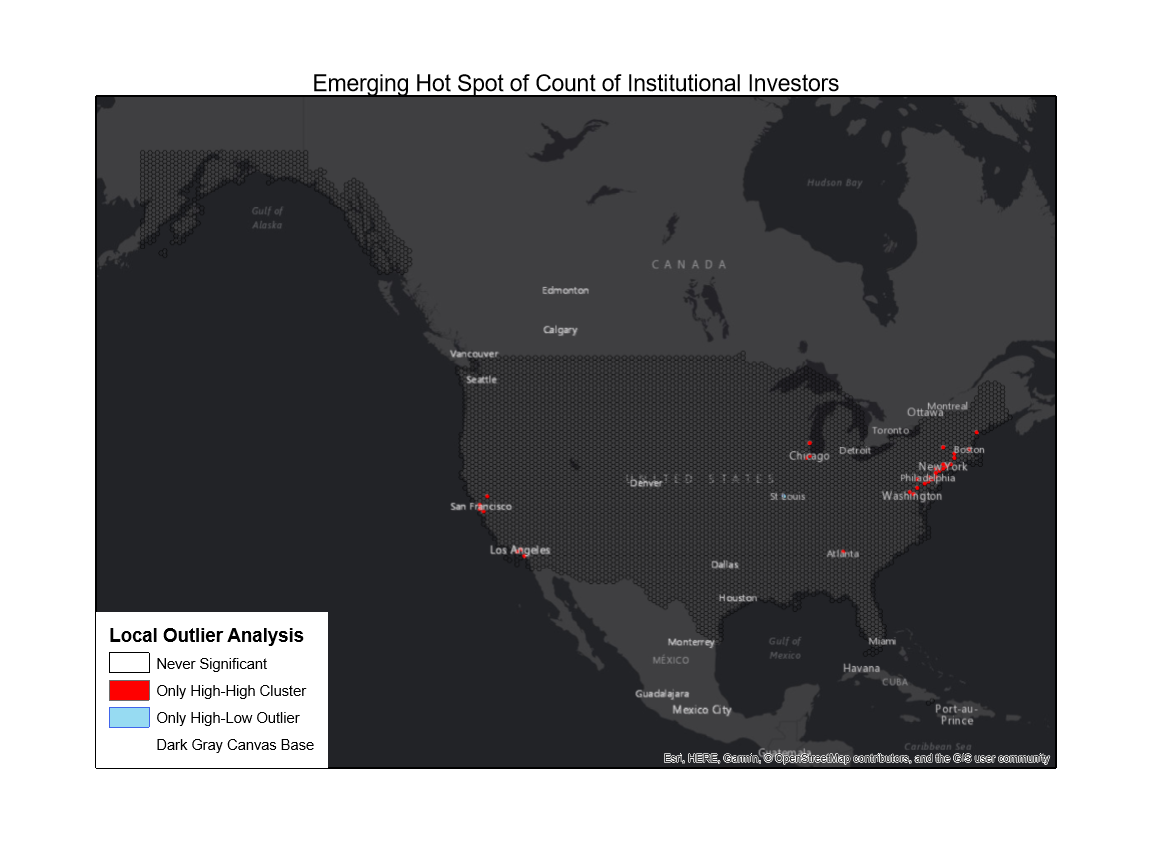
\includegraphics[width=\linewidth]{Figures/ChapterIV/USA_LOA_Money}
	\caption[Local Outlier Analysis For Funds under Management in the United States]{Local outlier analysis for funds under management in the United States for the Time Period of June 2013 to December 2018.}
	\label{fig:usaloamoney}
\end{figure}


\section{Boston}
\label{subsection:Boston}	
As seen in the various tables and analysis in Chapter \ref{ChapterIIIb}, Boston consistently ranks at the second most important metro area in terms of count of institutional investors and funds under management.  The hex bins for the Boston analysis measure 1 km between horizontal parallels and use a local window radius of 8 km.  In order to make the comparisons between cities meaningful, this scheme of hexagonal grid  and local window size was kept across different metro areas (Chicago, Los Angeles, New York City, and San Francisco).  

\subsection{Count Data}

Figure \ref{fig:bostoncounthotspot} identifies a large cluster covering the areas of Central Boston as well as the southern tip of the Massachusetts Route 128 corridor between the suburban cities of Dedham, Needham and Wellsley.  This cluster essentially contains 3 different types of hot spots.  The first area of central Boston is classified as an intensifying hot spot. This indicates a very high rate of increase in density of institutional investors by hex bin in the area around Boston Commons in downtown Boston.  The second type of hot spot covers the outer periphery of central Boston, as well as the southern arc of Highway 128.  Lastly, the southern part of the community of Dedham contains a sporadic hot spot indicating that this zone sees intermittent changes in institutional investor count over time.  The inclusion of the southern part of the route 128 high tech corridor in the investment cluster isn't surprising considering the long history of partnership between high tech research and development and finance capital \citep{kenney1999technology}.  

\begin{figure}
	\centering
	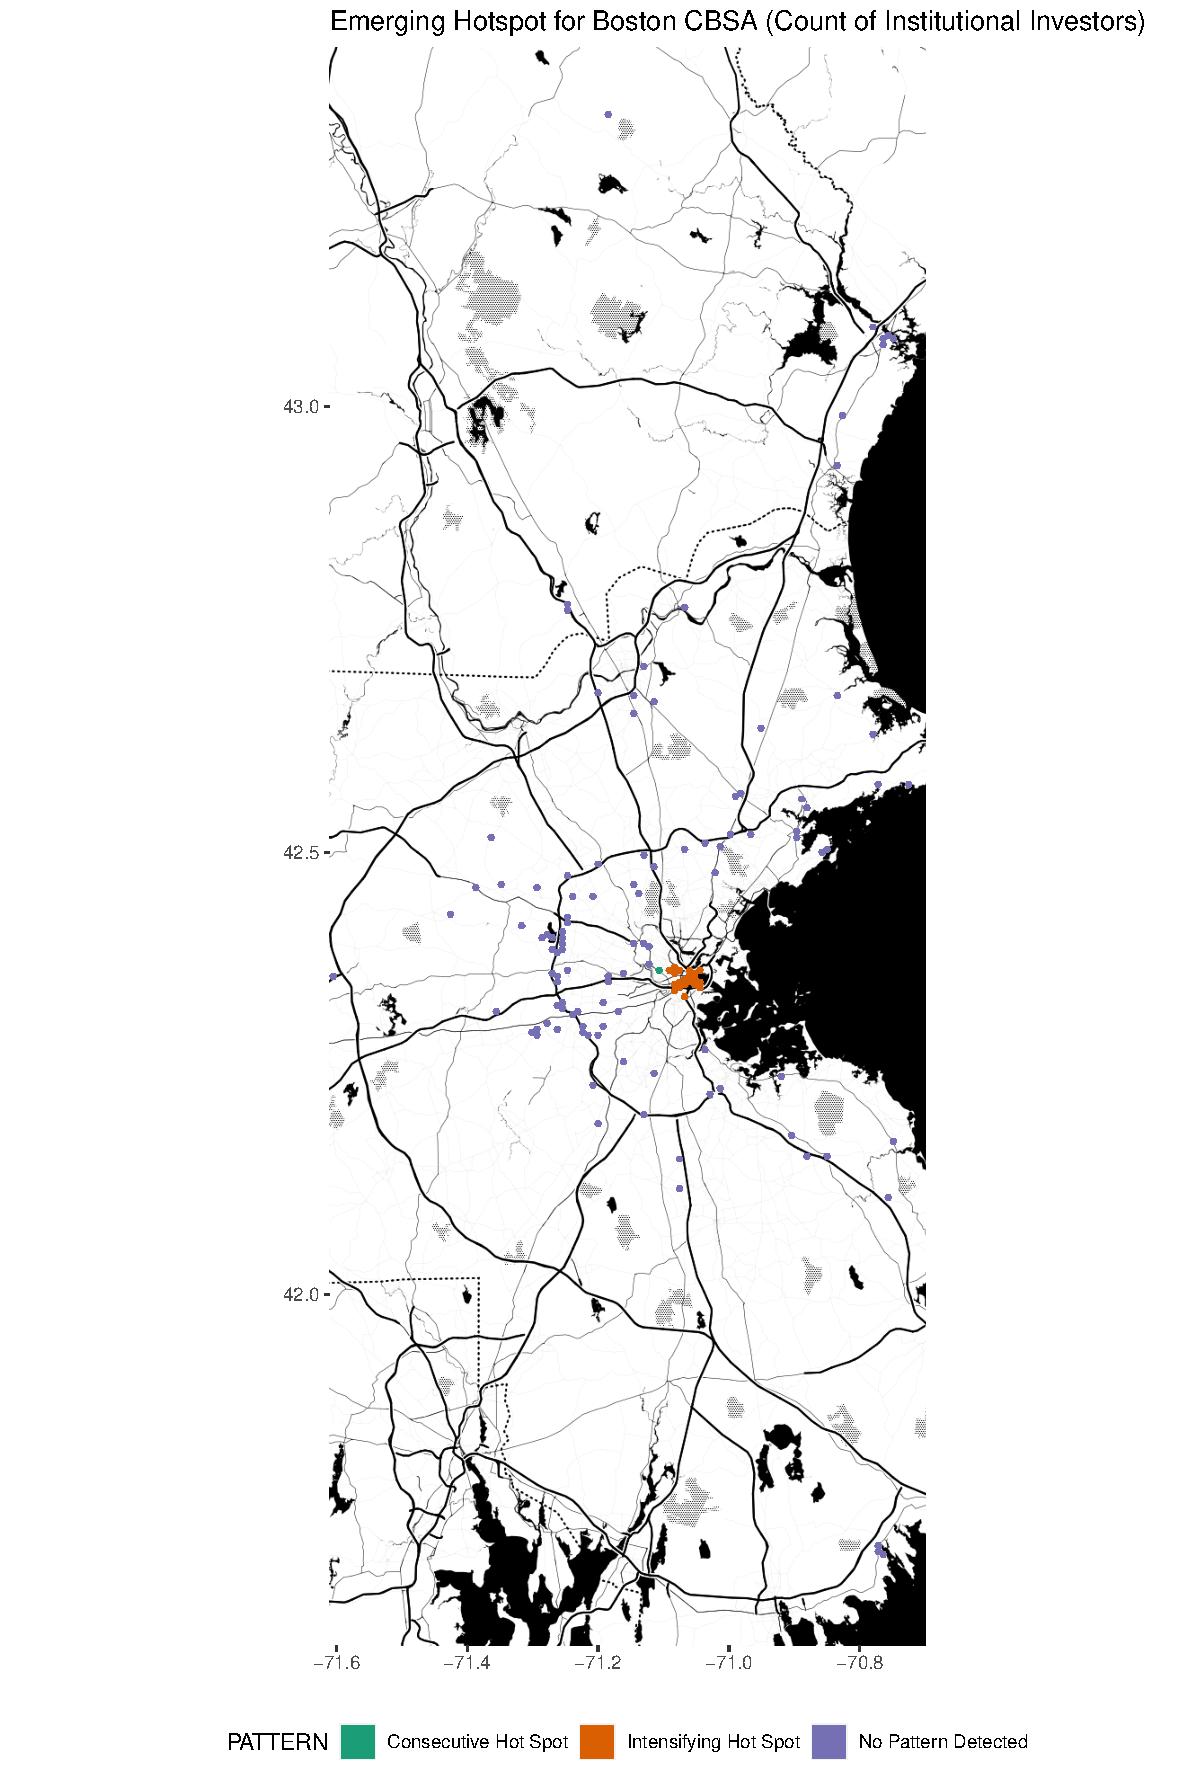
\includegraphics[width=1\linewidth]{Figures/ChapterIV/Bos_Count_EH}
	\caption[Hot Spot Analysis of Number of Firms in Boston]{Hot Spot Analysis of Number of Firms in Boston for the time period March 1999 to December 2018}
	\label{fig:bostoncounthotspot}
\end{figure}

Figure \ref{fig:bostoncountlocaloutliercount} displays of local outlier analysis confirms the importance of both central Boston as well as the southern arch of the route 128 corridor.   	

\begin{figure}
	\centering
	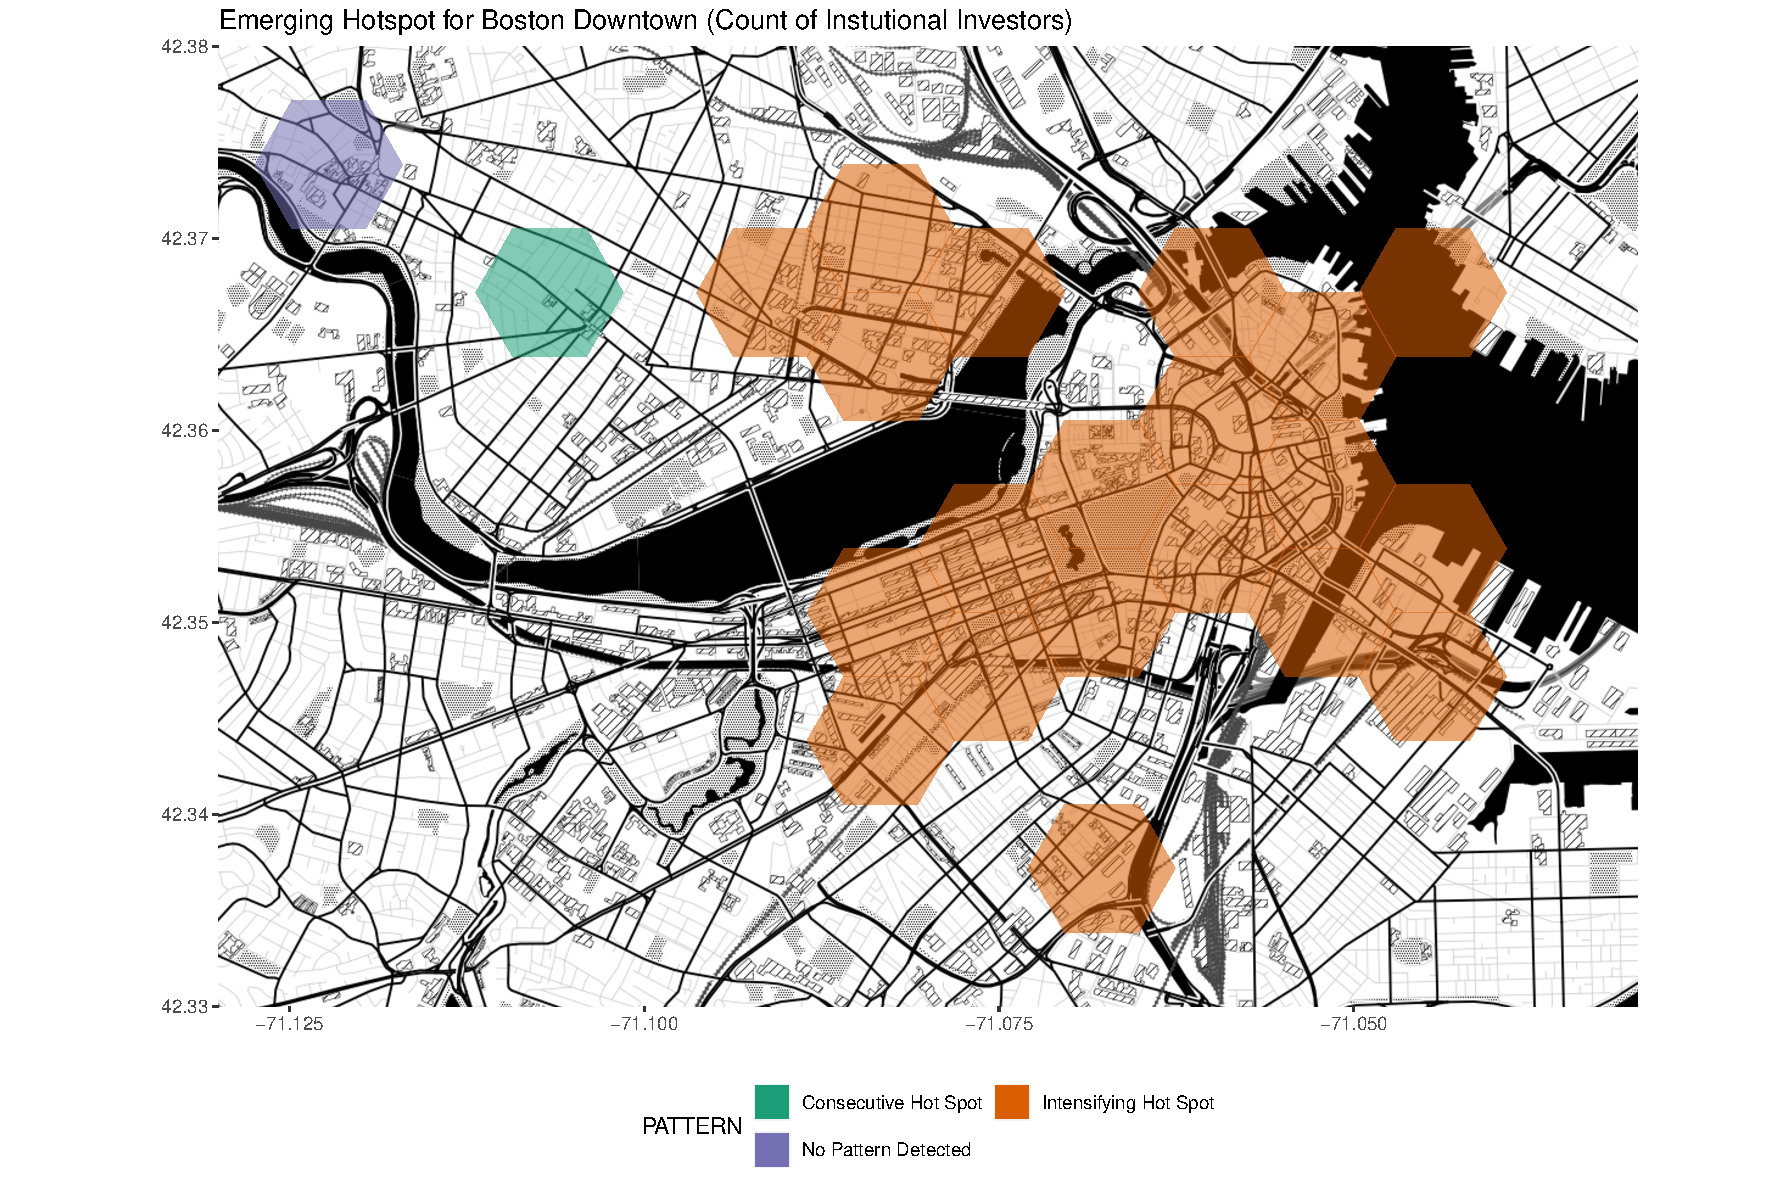
\includegraphics[width=1\linewidth]{Figures/ChapterIV/Bos_Count_EH_Downtown}
	\caption[Hot Spot Analysis of Number of Firms in Downtown Boston]{Hot Spot Analysis of Number of Firms in Downtown Boston for the time period March 1999 to December 2018}
	\label{fig:bostoncounthotspot_Downtown}
\end{figure}

\begin{figure}
	\centering
	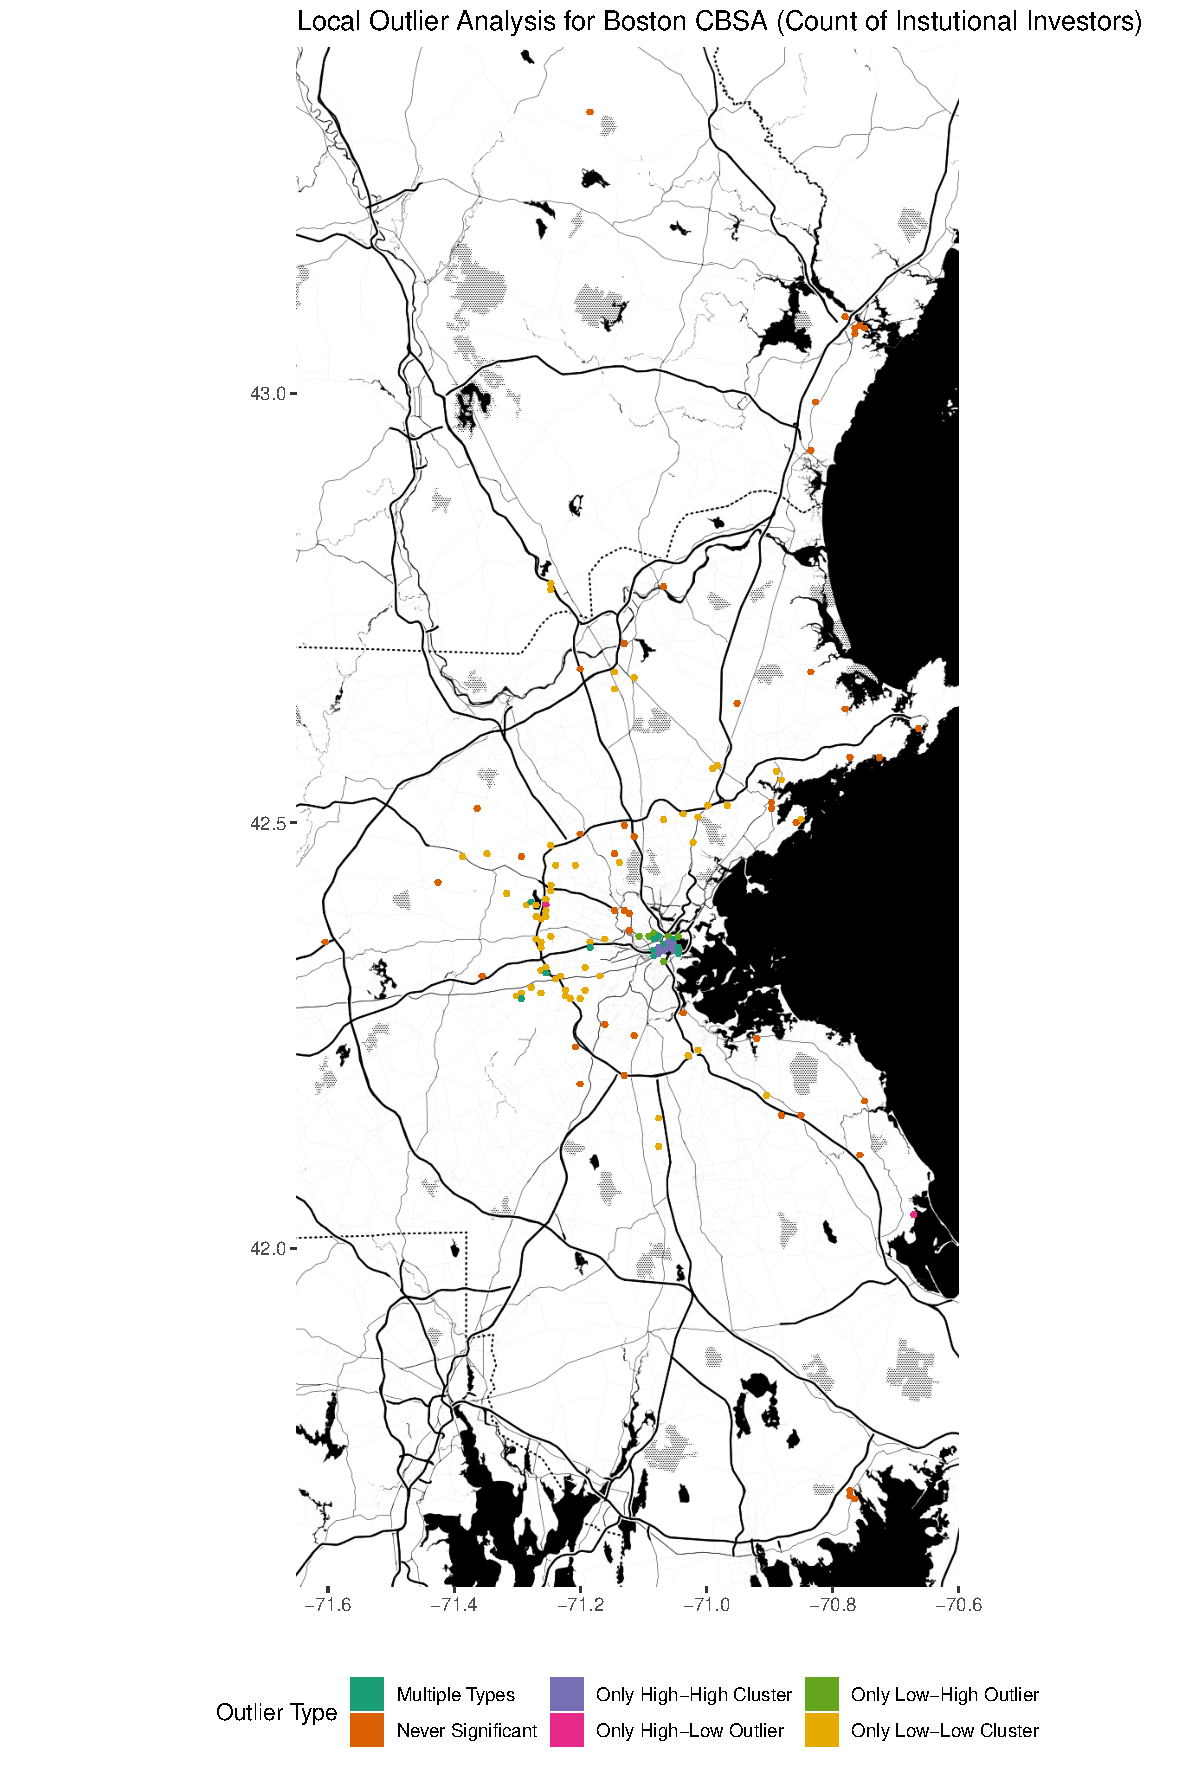
\includegraphics[width=1\linewidth]{Figures/ChapterIV/Bos_Count_LO}
	\caption[Boston Local Outlier Analysis - Count of Institutional Investors]{Boston Local Outlier Analysis - Count of Institutional Investors}
	\label{fig:bostoncountlocaloutliercount}
\end{figure}

\begin{figure}
	\centering
	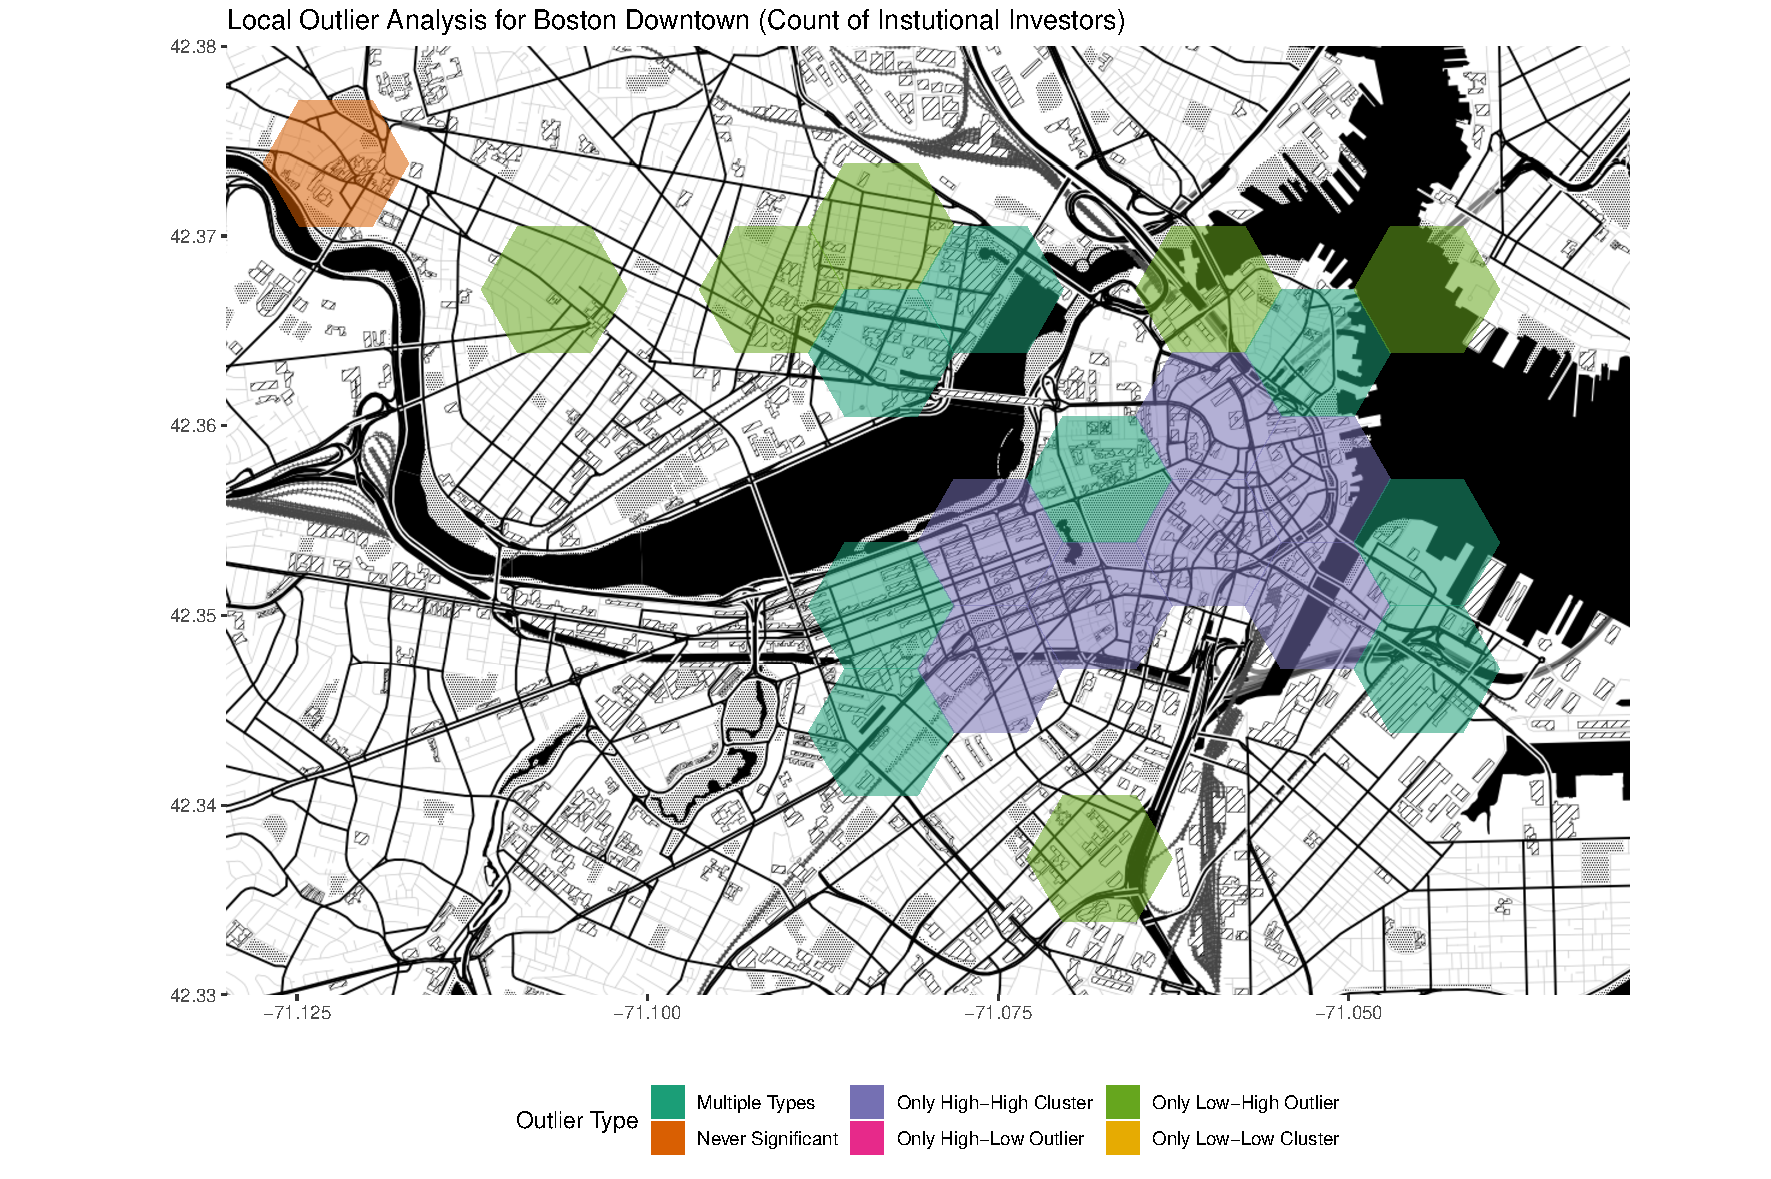
\includegraphics[width=1\linewidth]{Figures/ChapterIV/Bos_Count_LO_Downtown}
	\caption[Downtown Boston Local Outlier Analysis - Count of Institutional Investors]{Downtown Boston Local Outlier Analysis - Count of Institutional Investors}
	\label{fig:bostoncountlocaloutliercount_Downtown}
\end{figure}


\subsection{Funds under Management}

Unlike Figure \ref{fig:bostoncounthotspot}'s larger cluster, the emerging hot spot analysis in Figure \ref{fig:bostonmoneyhotspot} using funds under management as a criteria is more exclusionary since it only contains central Boston, and ignores the Massachusetts Route 128 corridor.  A partial explanation for this is the high collection of bank and insurance based institutional investors located in Boston's financial district that abuts Boston Common .    	

\begin{figure}
	\centering
	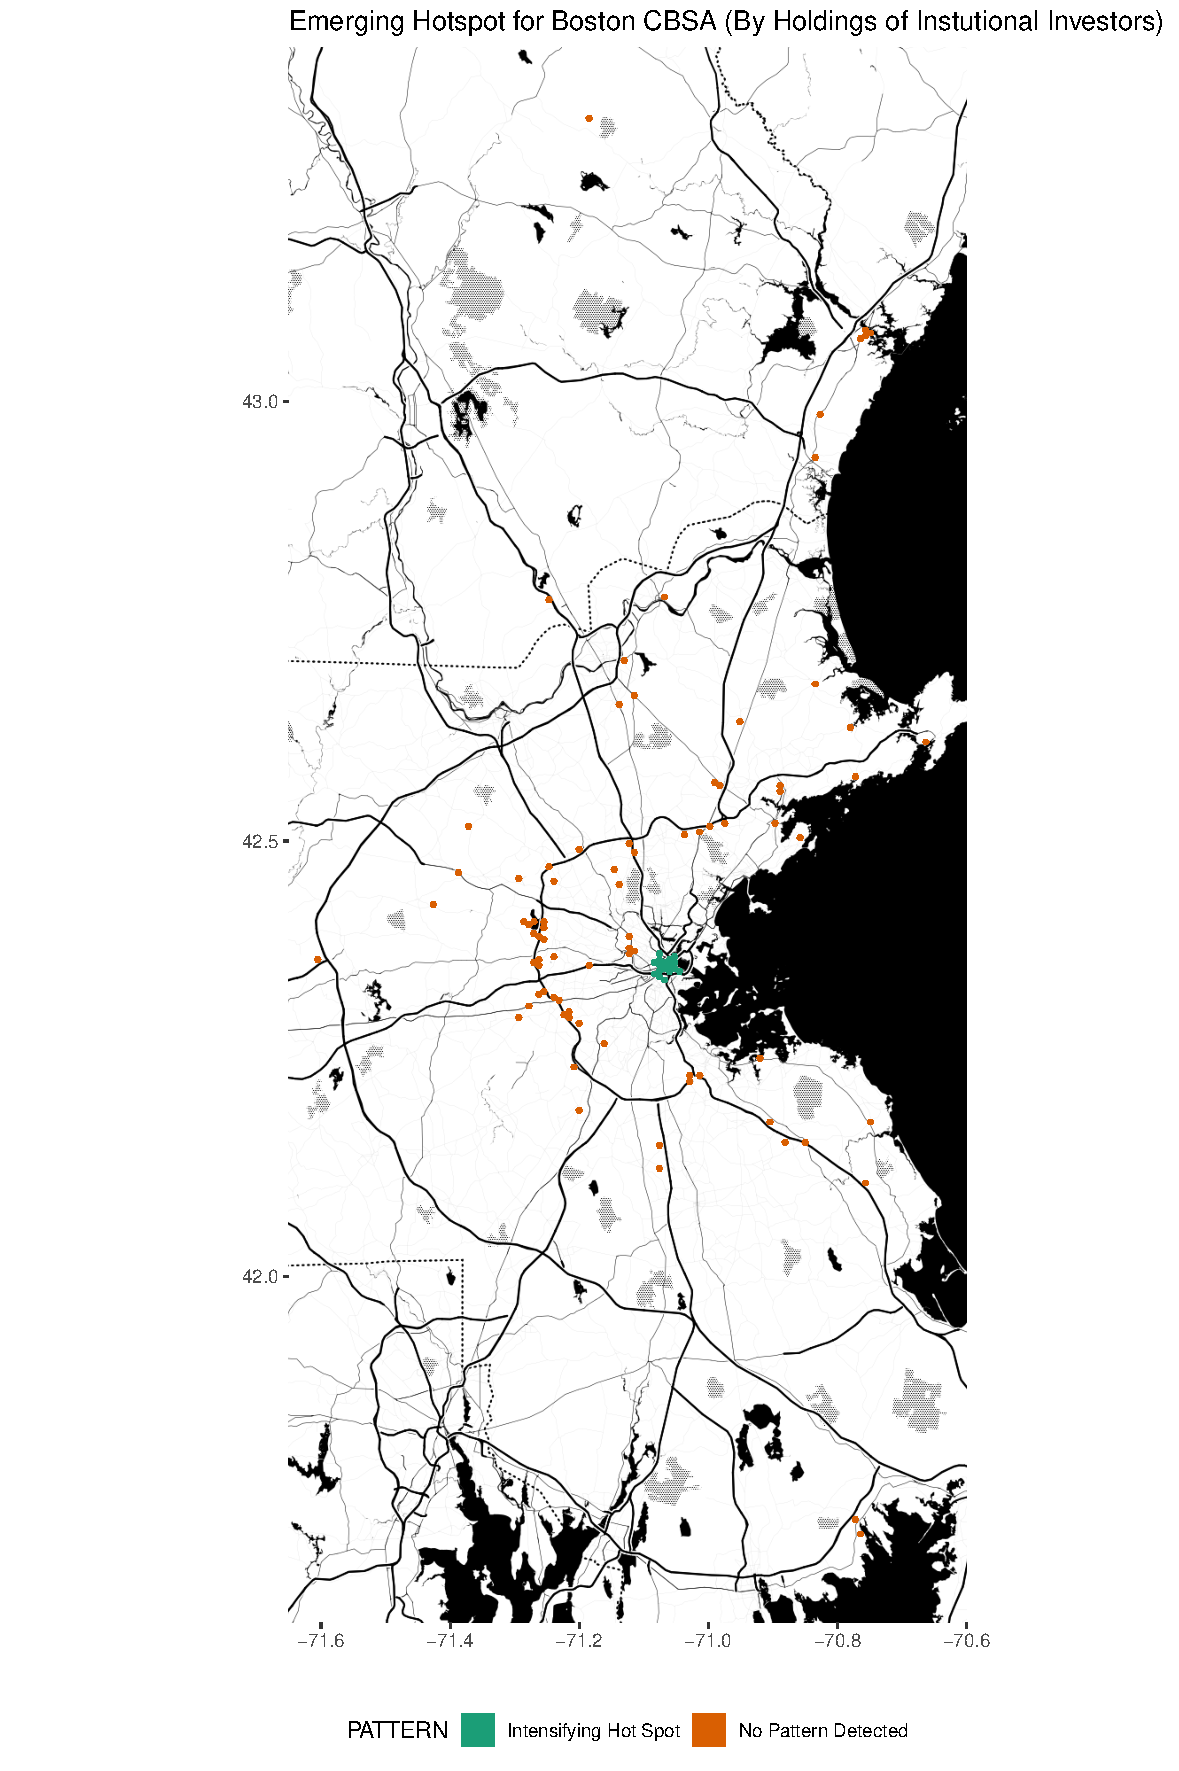
\includegraphics[width=1\linewidth]{Figures/ChapterIV/Bos_Money_EH}
	\caption[Emerging Hot Spot Analysis of Funds under Management for Boston]{Emerging Hot Spot Analysis of Funds under Management for Boston for period June 2013 to December 2018}
	\label{fig:bostonmoneyhotspot}
\end{figure}

\begin{figure}
	\centering
	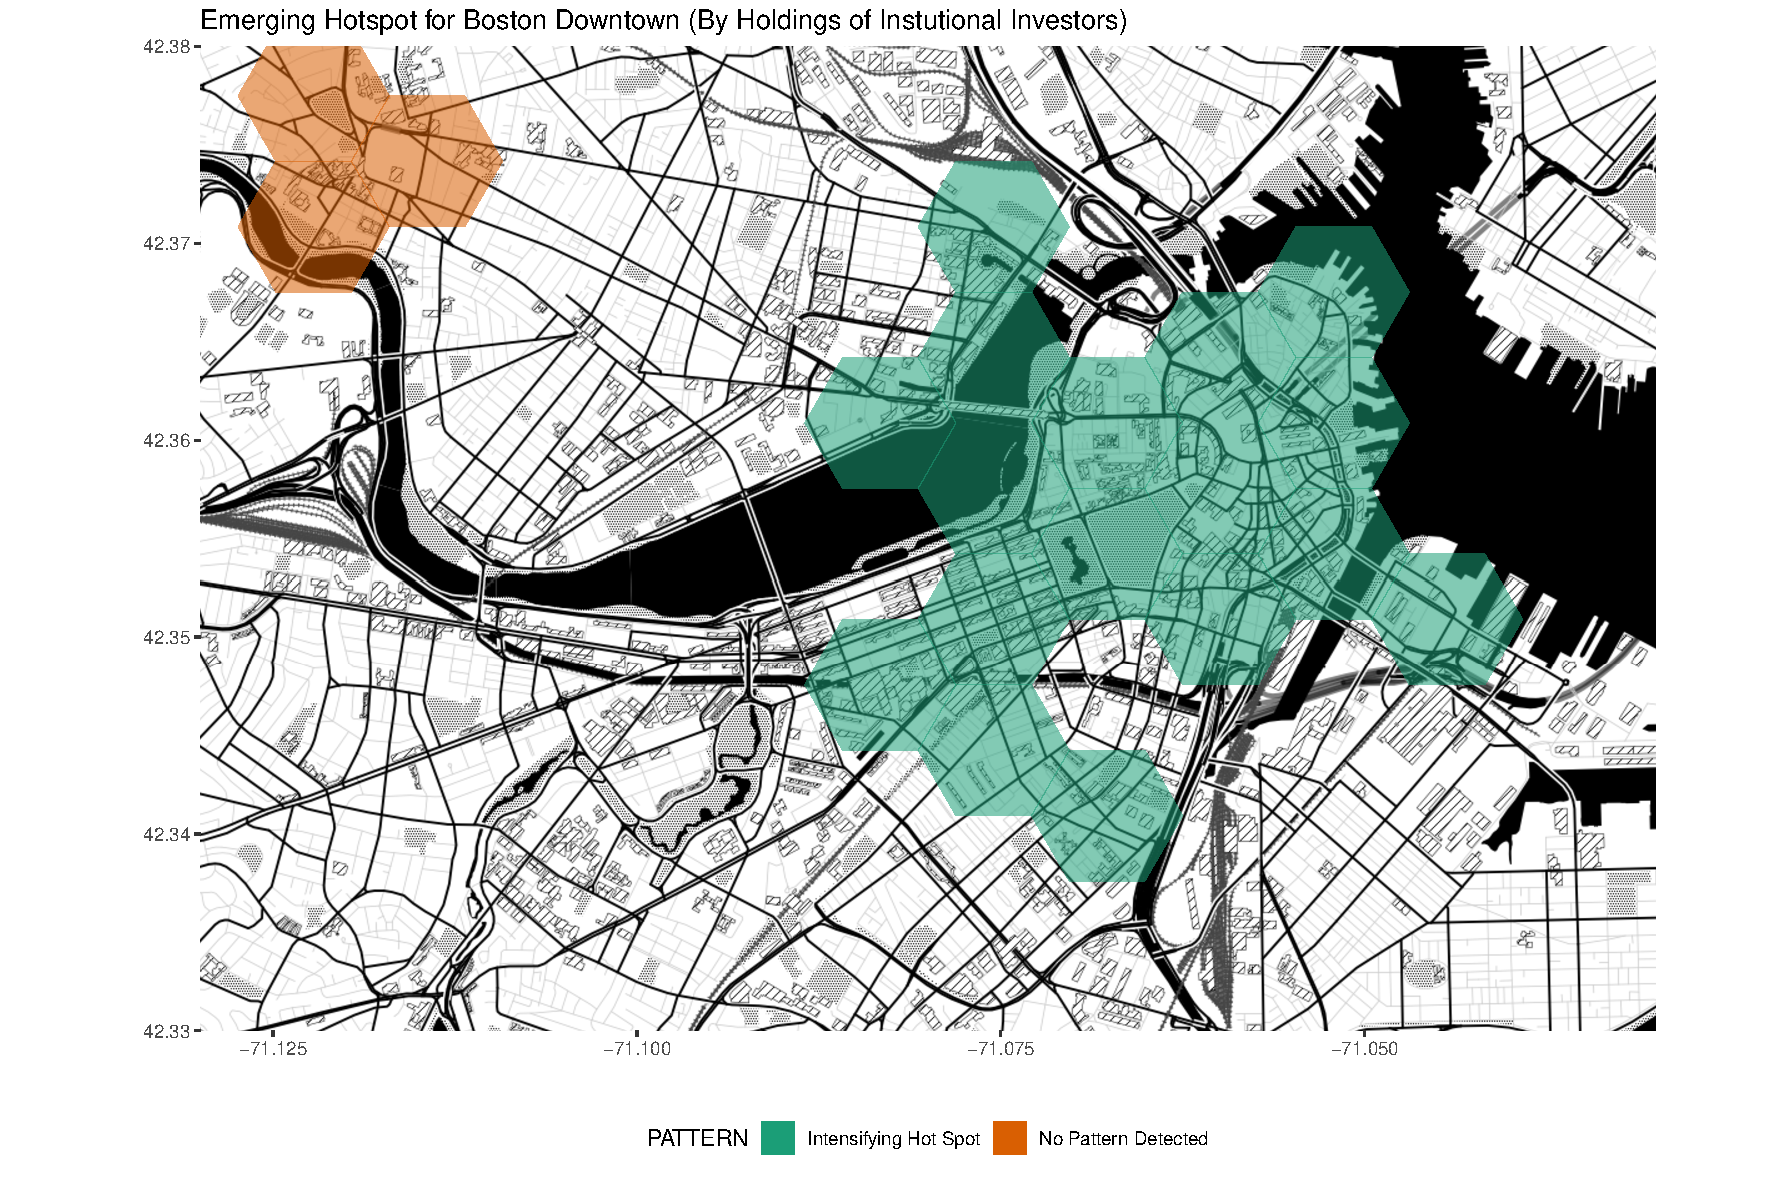
\includegraphics[width=1\linewidth]{Figures/ChapterIV/Bos_Money_EH_Downtown}
	\caption[Emerging Hot Spot Analysis of Funds under Management for Downtown Boston]{Emerging Hot Spot Analysis of Funds under Management for Downtown Boston for period June 2013 to December 2018}
	\label{fig:bostonmoneyhotspot_Downtown}
\end{figure}


Following in a similar theme to Figure \ref{fig:bostonmoneyhotspot}, the local outlier analysis only finds high-high clusters in central Boston. Interestingly, the model accurately picks out Boston Common as a non-cluster.  A look at the region shows that many institutional investors surround this 25 hectare urban park, and this creates a discontinuity.  

\begin{figure}
	\centering
	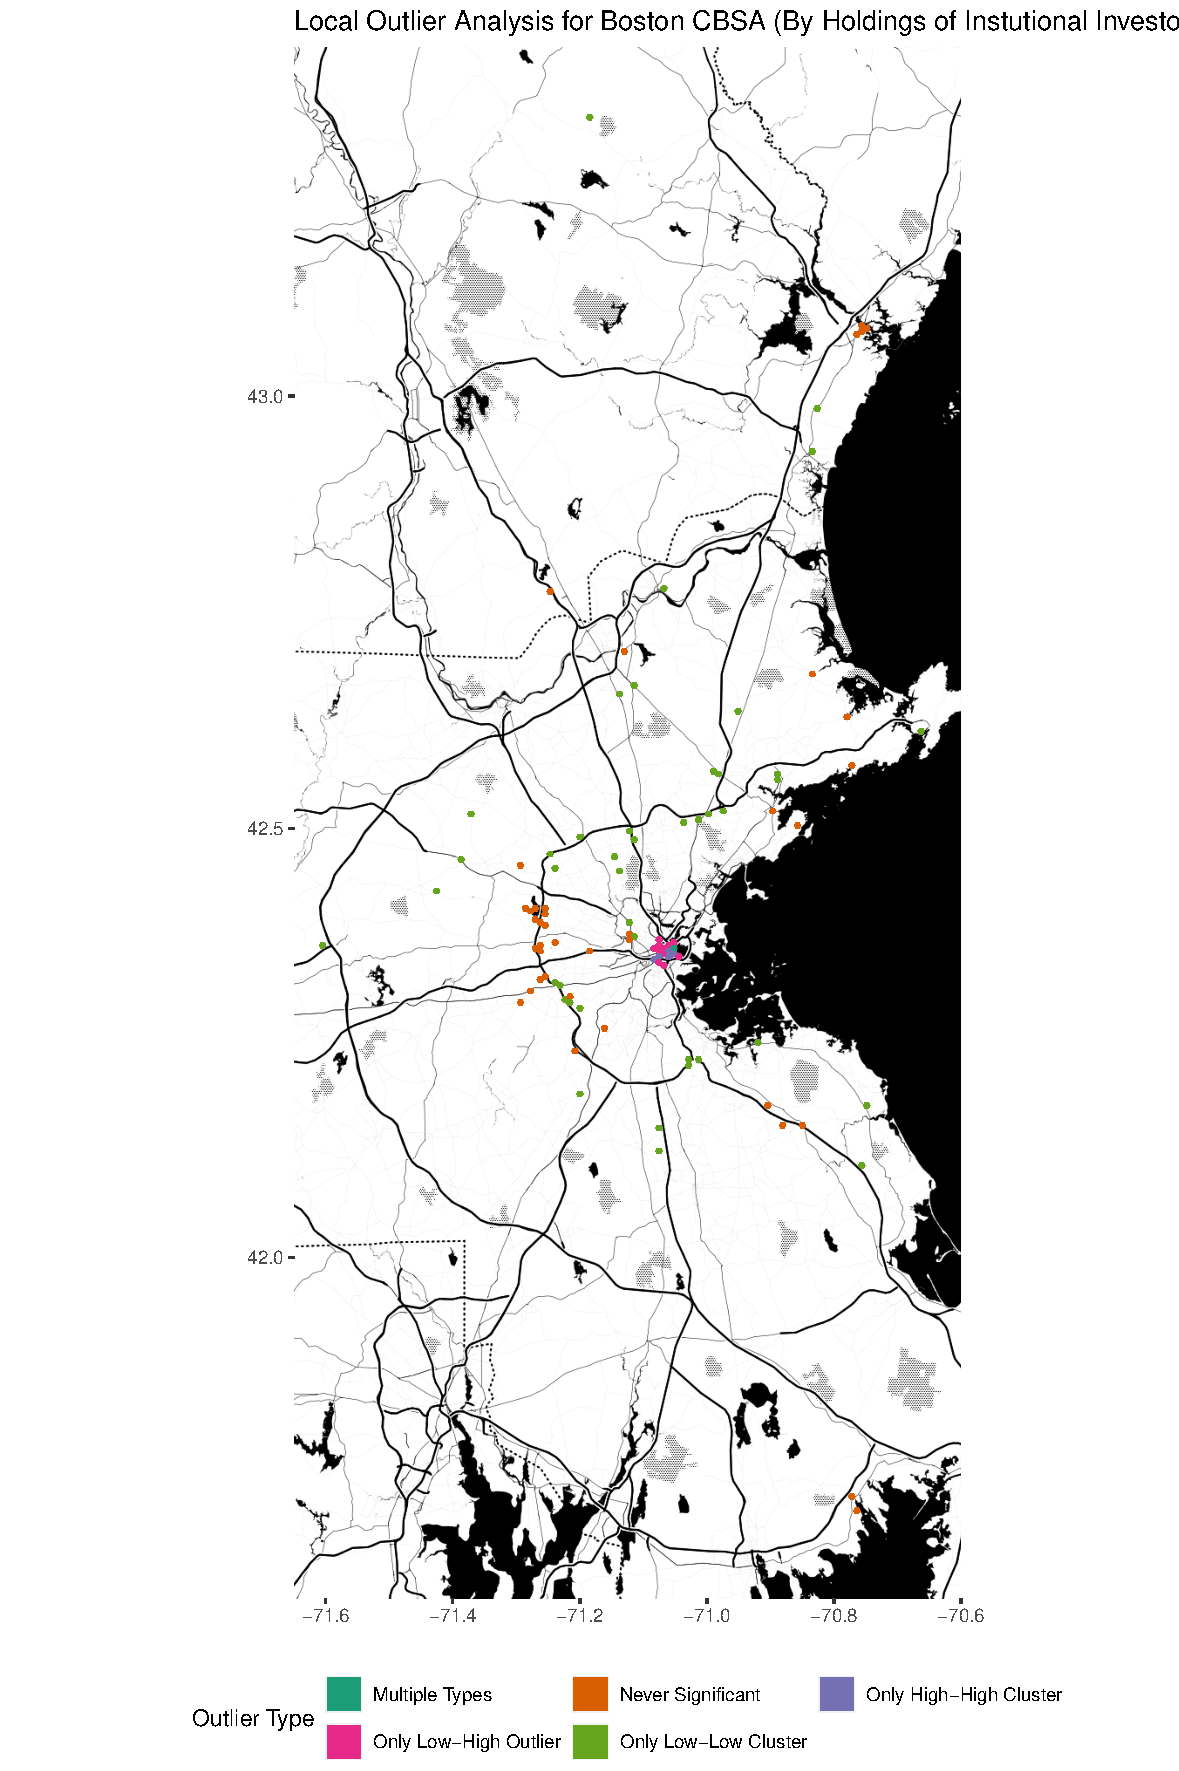
\includegraphics[width=1\linewidth]{Figures/ChapterIV/Bos_Money_LO}
	\caption[Boston Local Outlier Analysis - Funds under Management]{Boston Local Outlier Analysis - Funds under Management}
	\label{fig:bostonlocaloutlier}
\end{figure}


\begin{figure}
	\centering
	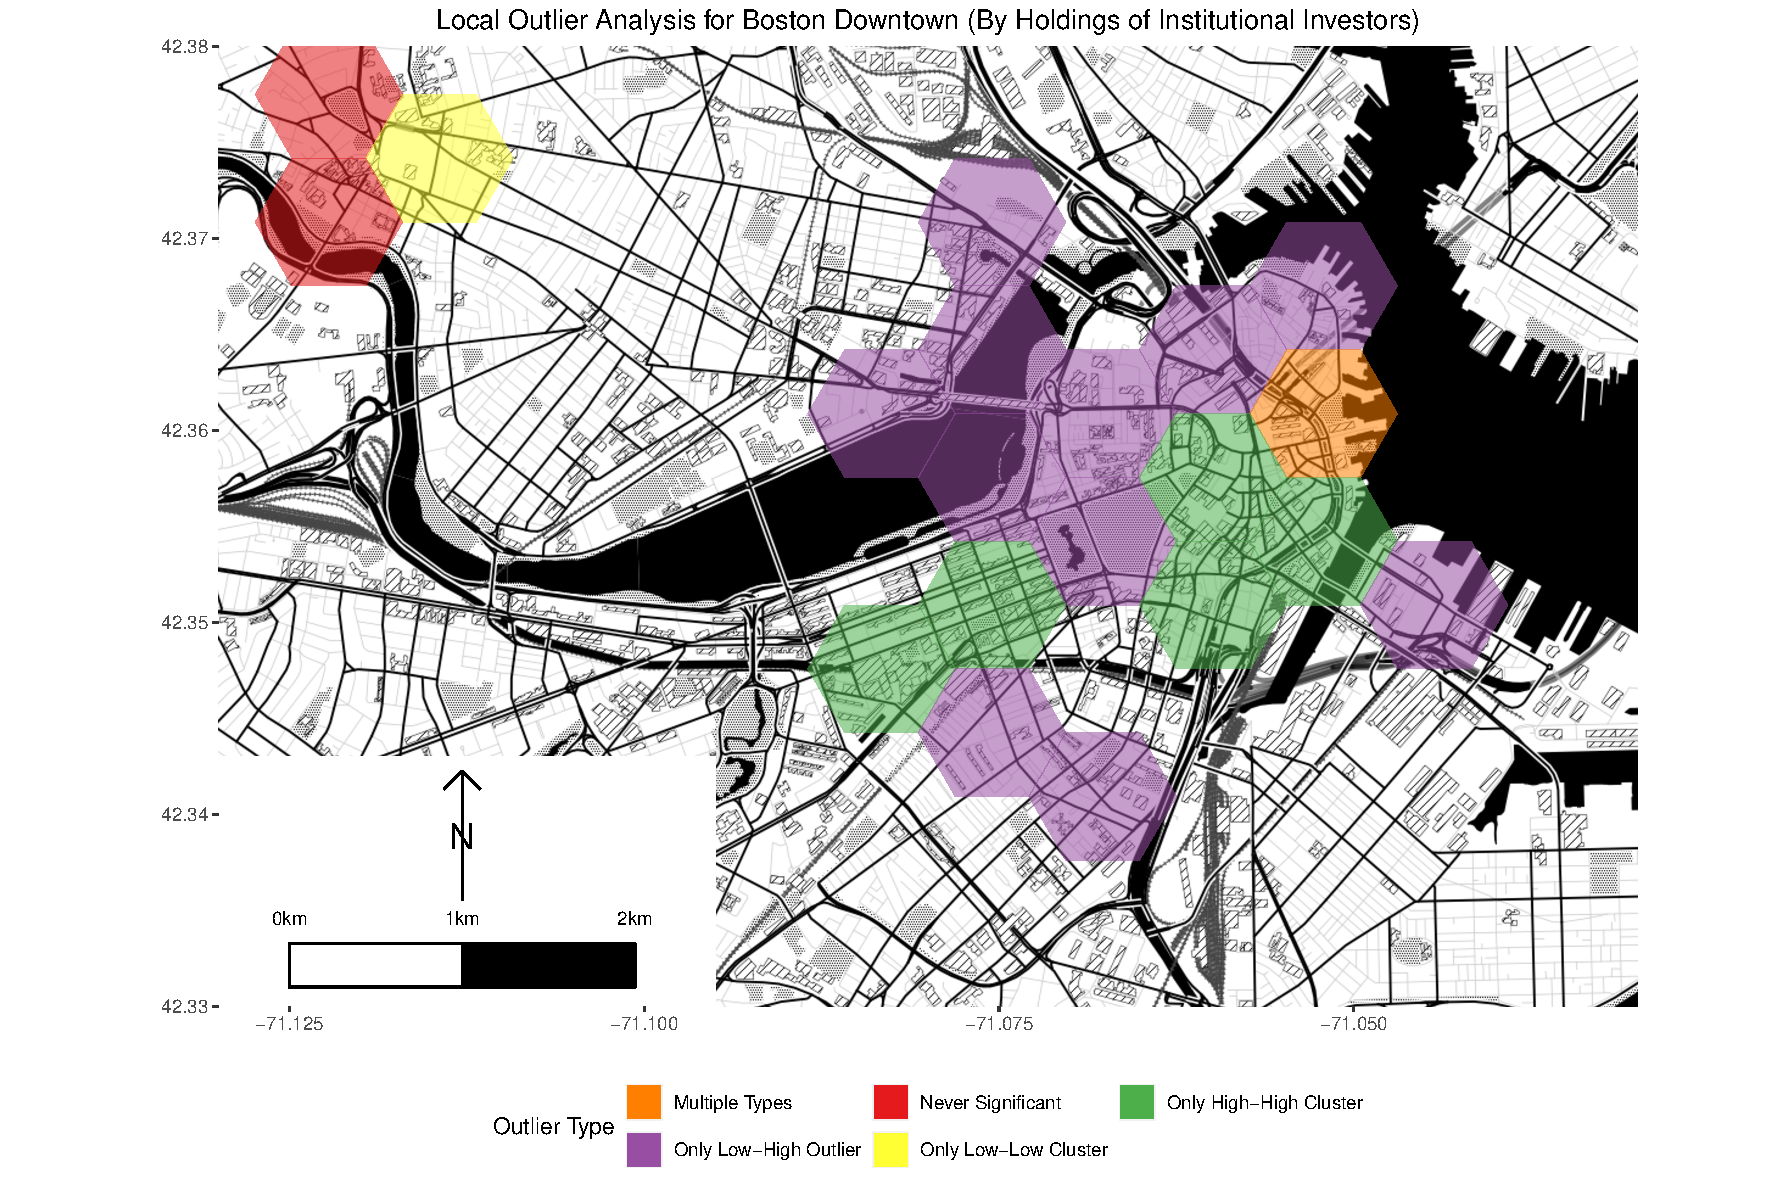
\includegraphics[width=1\linewidth]{Figures/ChapterIV/Bos_Money_LO_Downtown}
	\caption[Boston Downtown Local Outlier Analysis - Funds under Management]{Boston Downtown Local Outlier Analysis - Funds under Management}
	\label{fig:bostonlocaloutlier_Downtown}
\end{figure}



\section{Chicago}

\subsection{Count Data}
As displayed in Figure \ref{fig:Chicagocounthotspot}, Chicago contains one intensifying hot spot in the Chicago Loop neighbourhood, including satellite hot spots in the Napierville-Aurora suburb to the West, as well as Evanston and Highland Park to the North.  
\begin{figure}
	\centering
	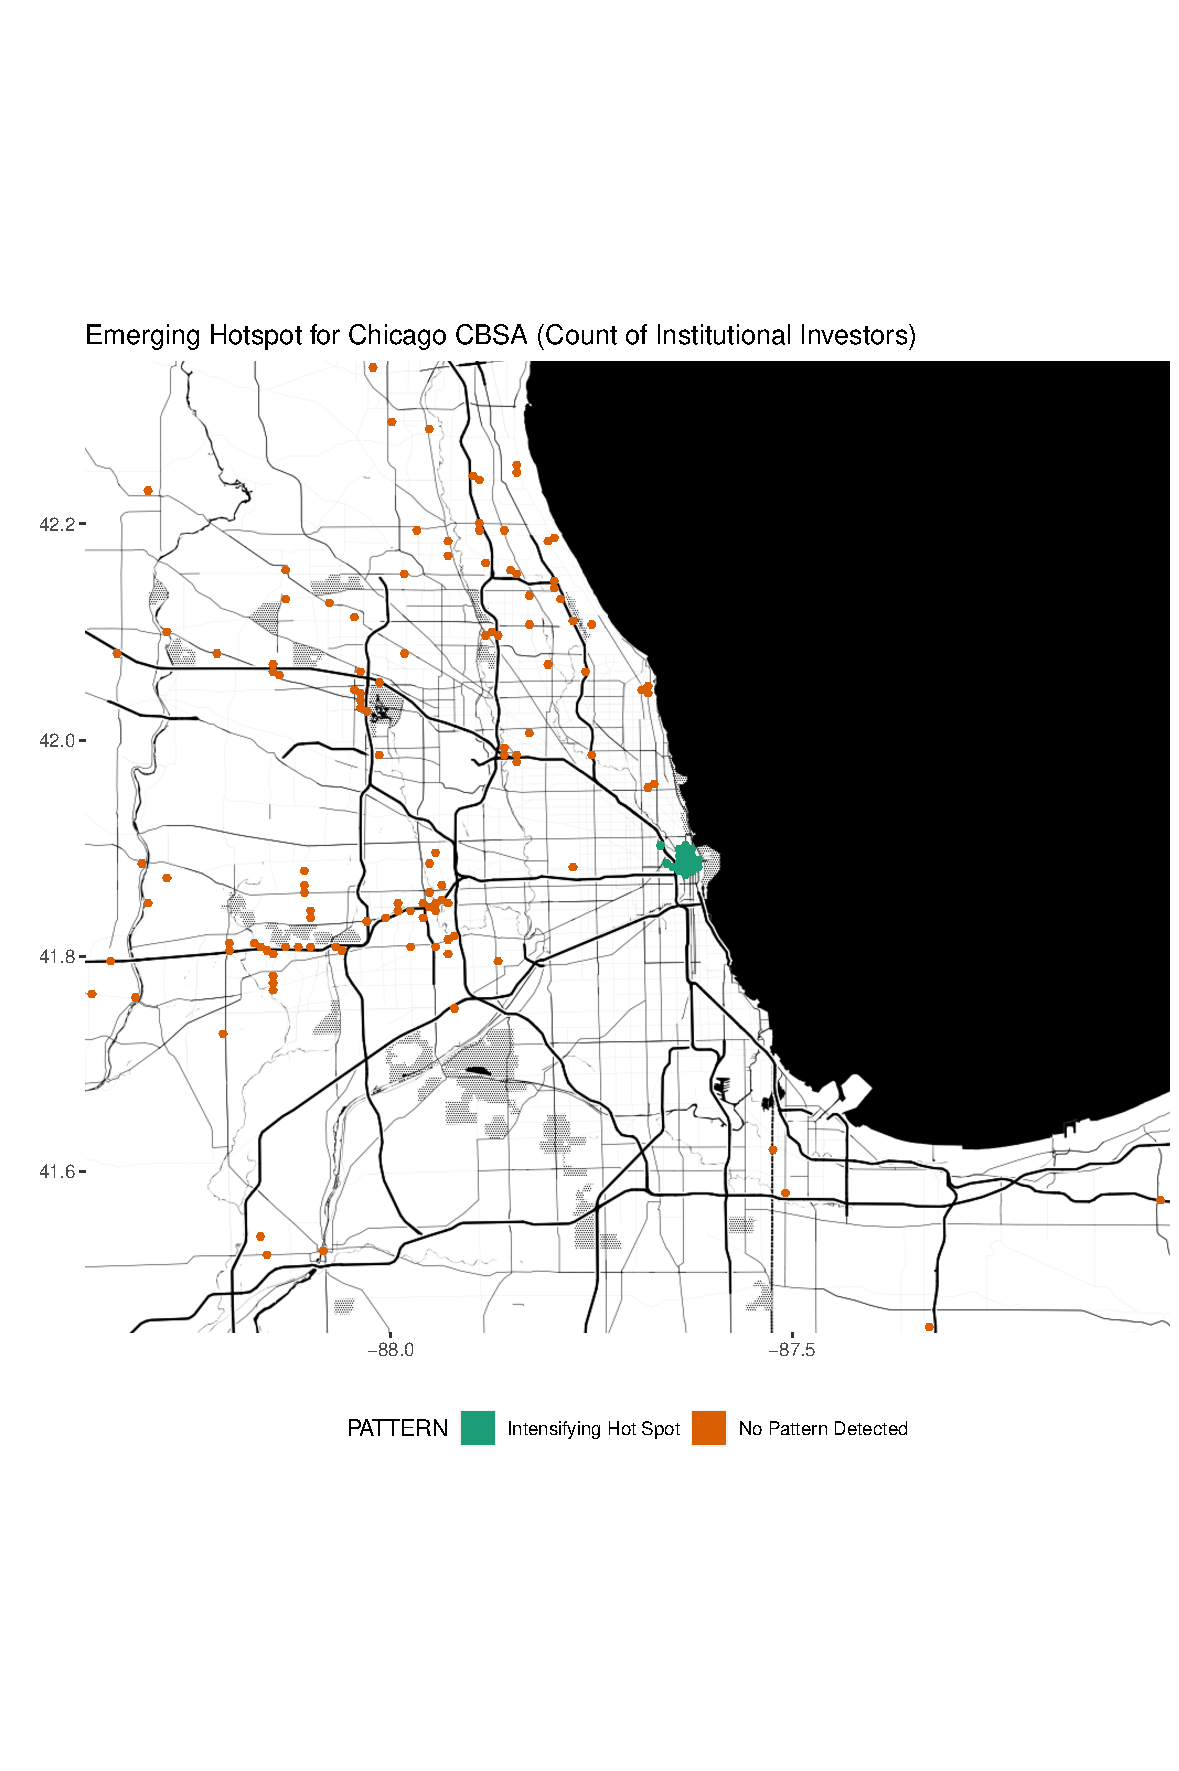
\includegraphics[width=1\linewidth]{Figures/ChapterIV/Chi_Count_EH}
	\caption[Hot Spot Analysis of Number of Firms in Chicago]{Hot Spot Analysis of Number of Firms in Chicago for the time period March 1999 to December 2018}
	\label{fig:Chicagocounthotspot}
\end{figure}

\begin{figure}
	\centering
	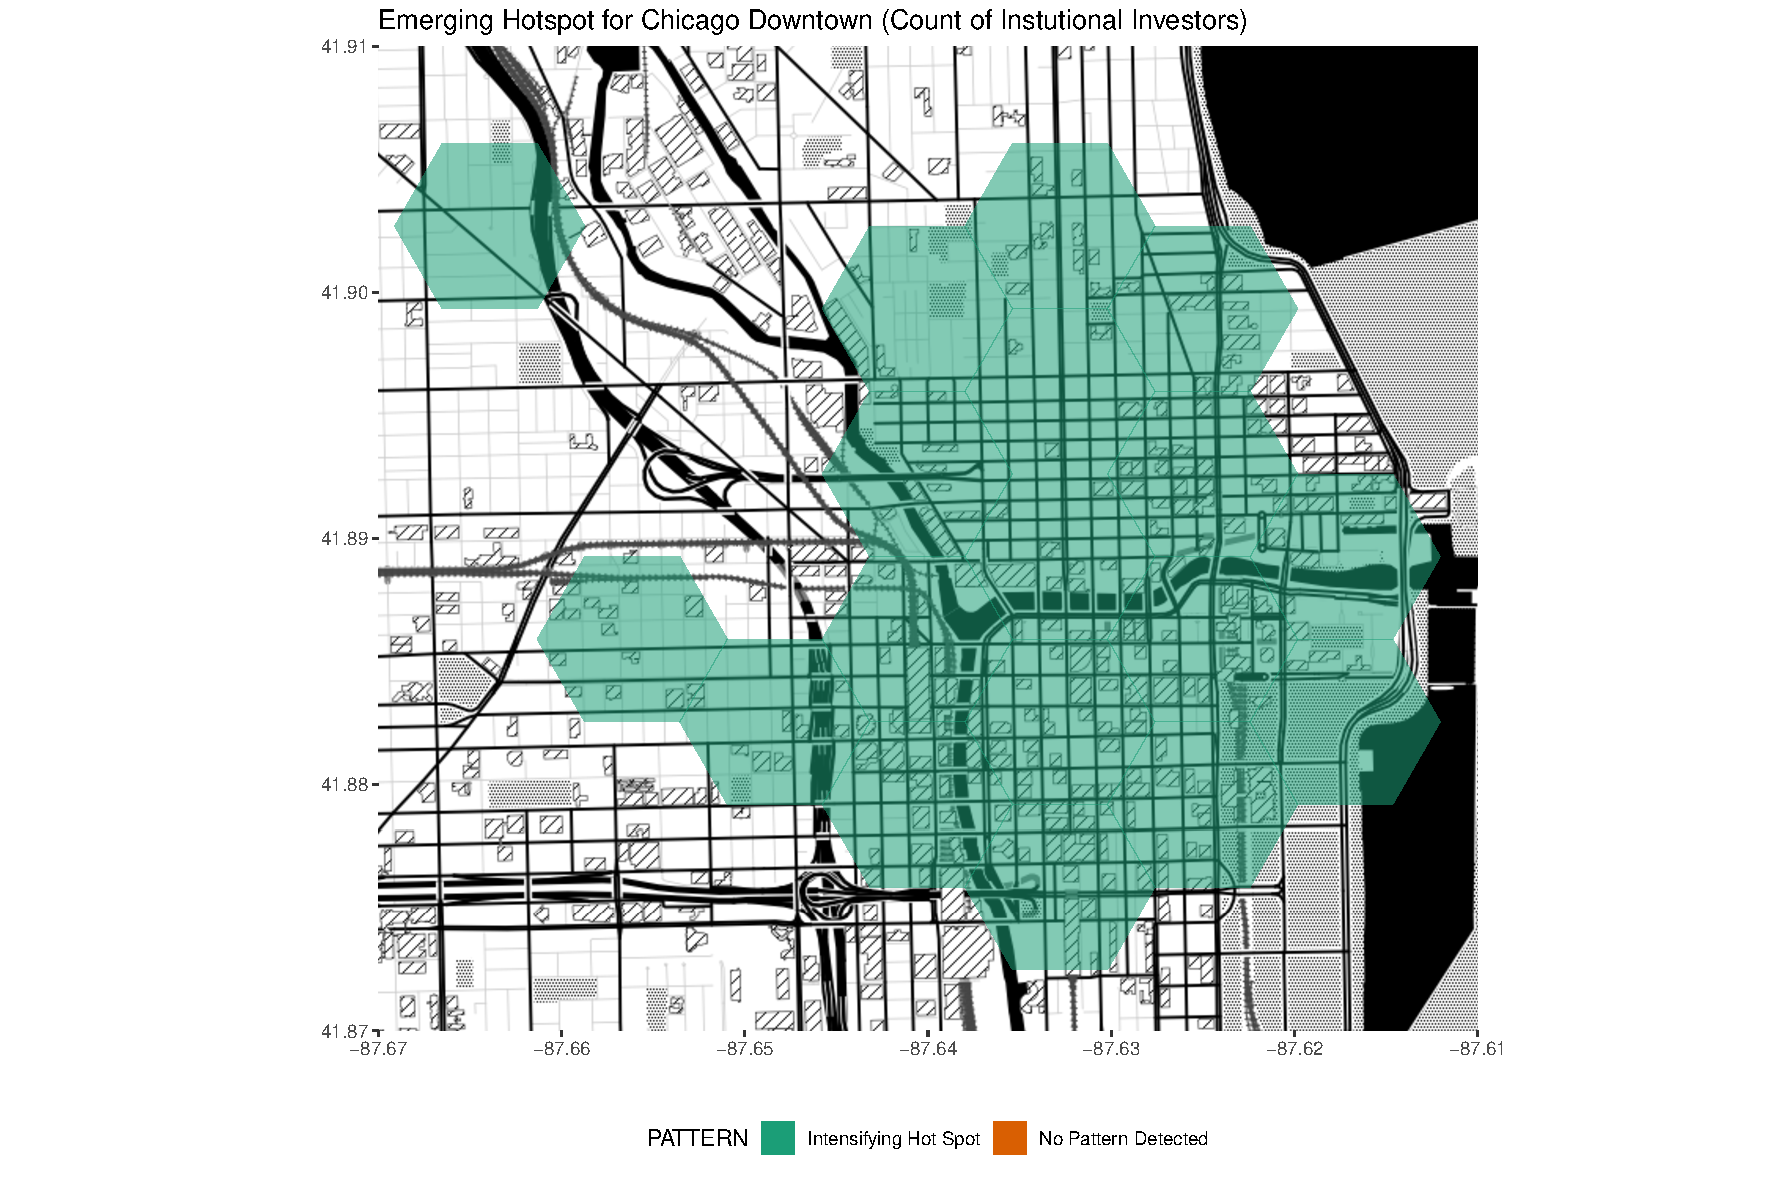
\includegraphics[width=1\linewidth]{Figures/ChapterIV/Chi_Count_EH_Downtown}
	\caption[Hot Spot Analysis of Number of Firms in Chicago]{Hot Spot Analysis of Number of Firms in Chicago for the time period March 1999 to December 2018}
	\label{fig:Chicagocounthotspot_Downtown}
\end{figure}


Using local outlier analysis, only the Loop district contains high-high hexagons. This is consistent with institutional investors perfering CBDs.  Futhermore, there is a conspicuous absence of investors on the South Side of Chicago, however this is not a region of Chicago known for having much financial capital.  
\begin{figure}
	\centering
	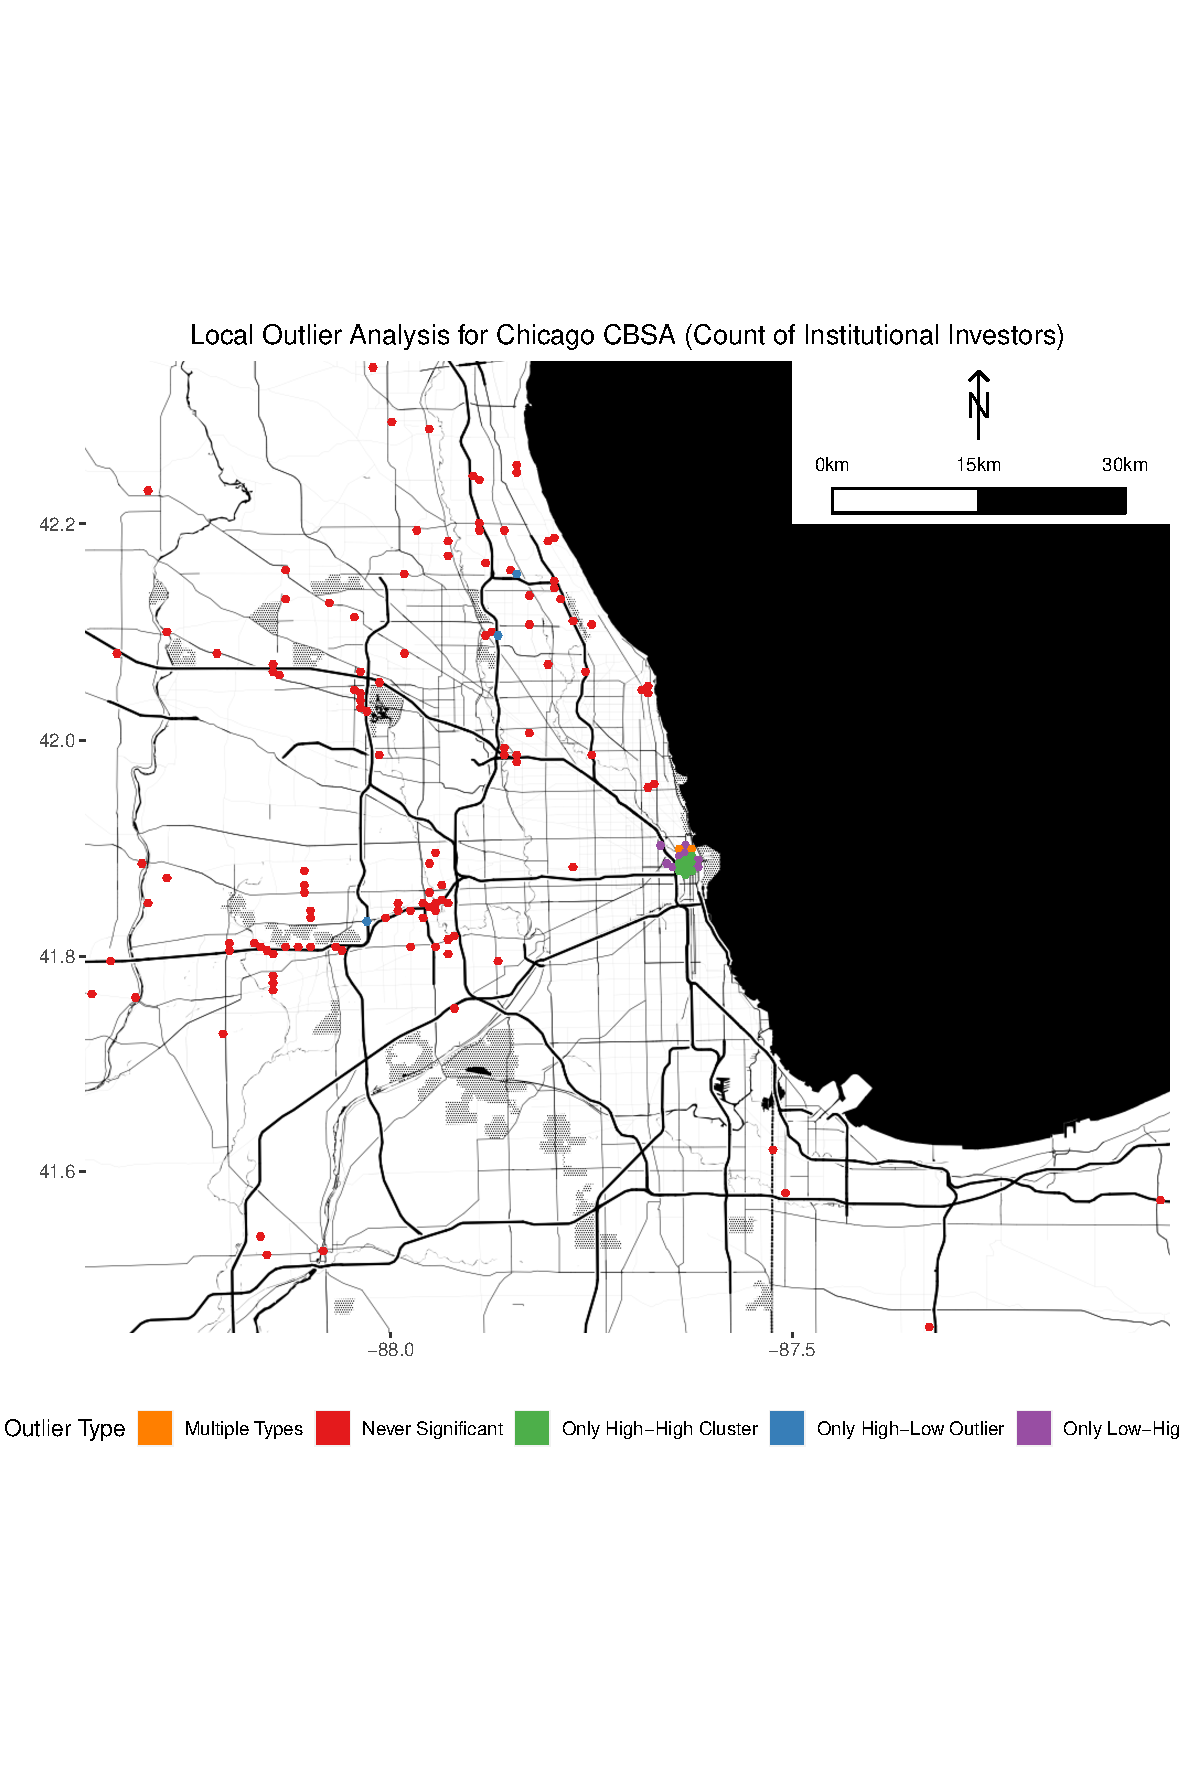
\includegraphics[width=1\linewidth]{Figures/ChapterIV/Chi_Count_LO}
	\caption[Chicago Local Outlier Analysis - Count of Institutional Investors]{Chicago Local Outlier Analysis - Count of Institutional Investors}
	\label{fig:Chicagocountlocaloutliercount}
\end{figure}	

\begin{figure}
	\centering
	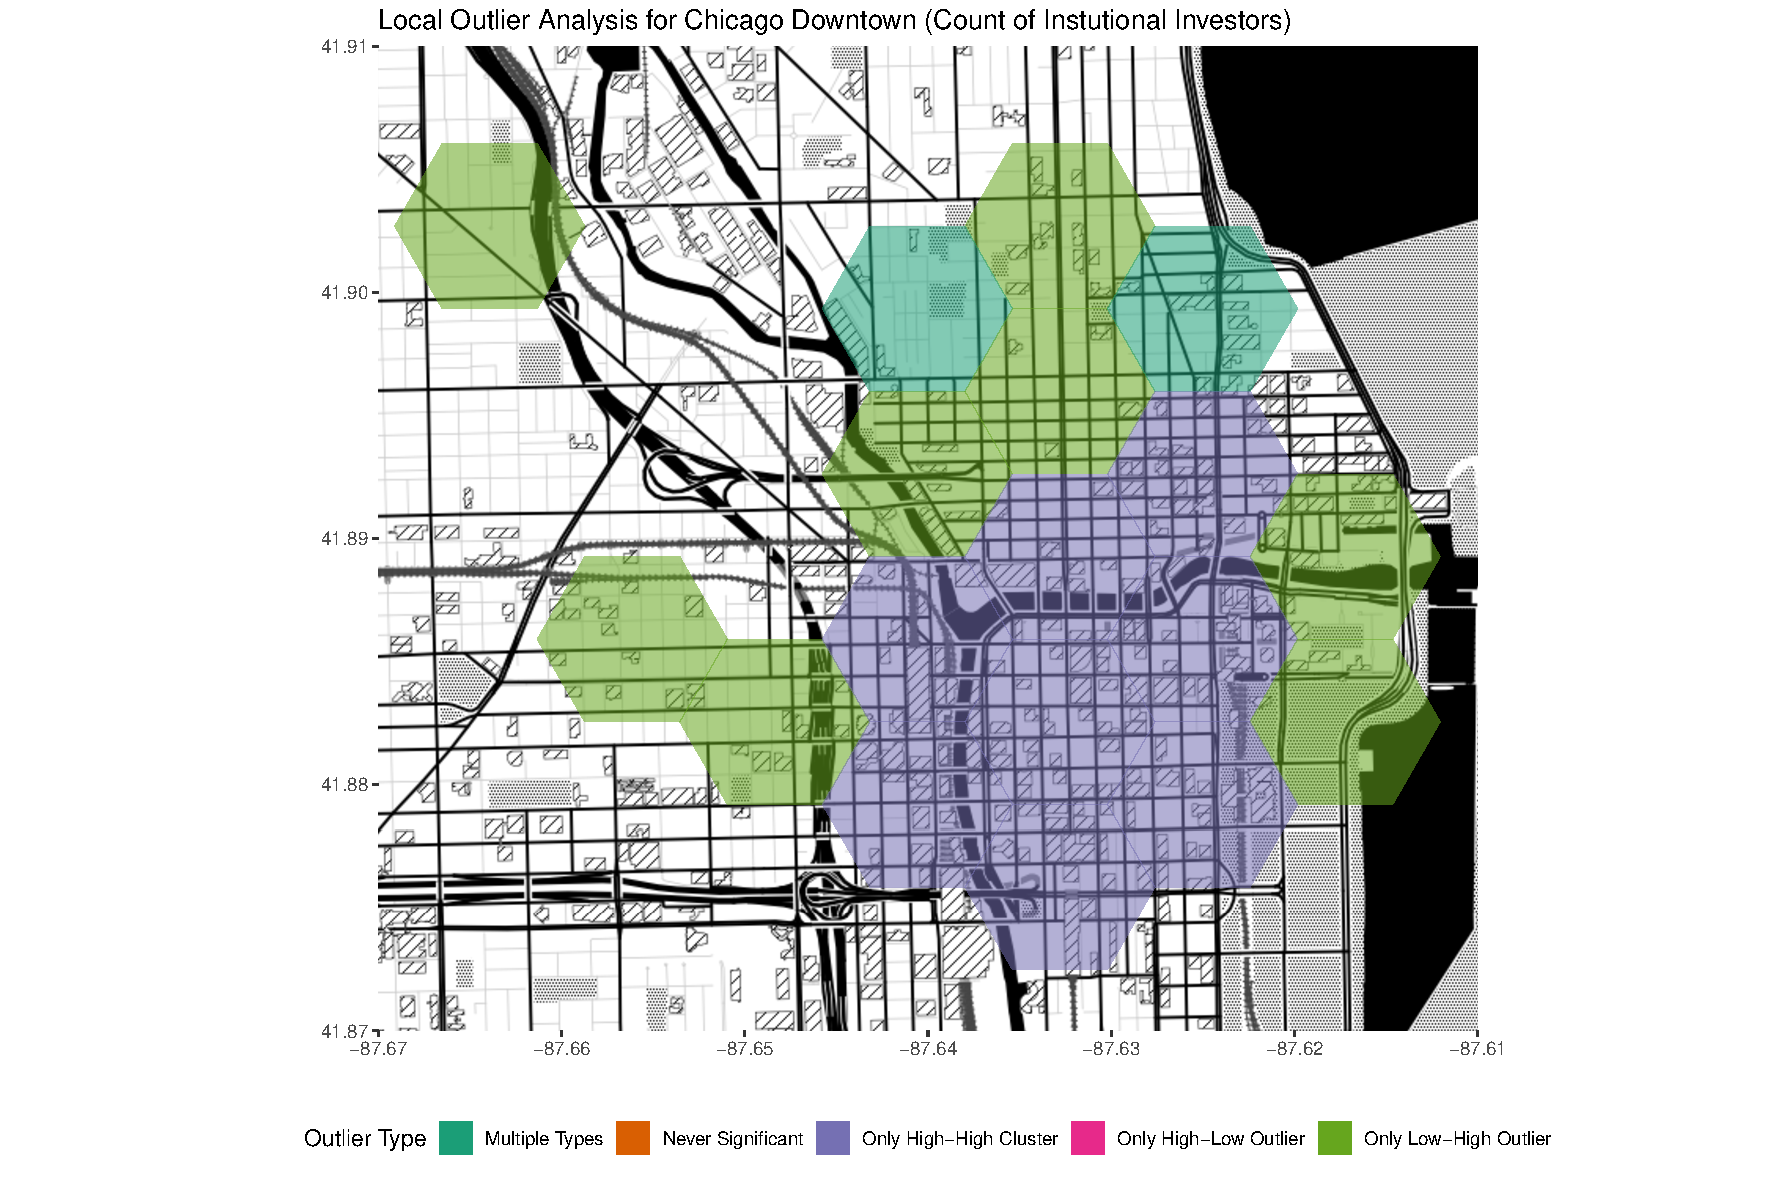
\includegraphics[width=1\linewidth]{Figures/ChapterIV/Chi_Count_LO_Downtown}
	\caption[Chicago Local Outlier Analysis - Count of Institutional Investors]{Chicago Local Outlier Analysis - Count of Institutional Investors}
	\label{fig:Chicagocountlocaloutliercount_Downtown}
\end{figure}	

\subsection{Funds under Management}

Figure \ref{fig:Chicagonmoneyhotspot} suggests a similar picture to the other emerging hot spot analysis maps where the key variable is funds under management, for there are less regions defined as a hot spot.  In this case, the hot spots in Evanston and Highland Park disappear, and the Napierville-Aurora cluster is much smaller in size.    

\begin{figure}
	\centering
	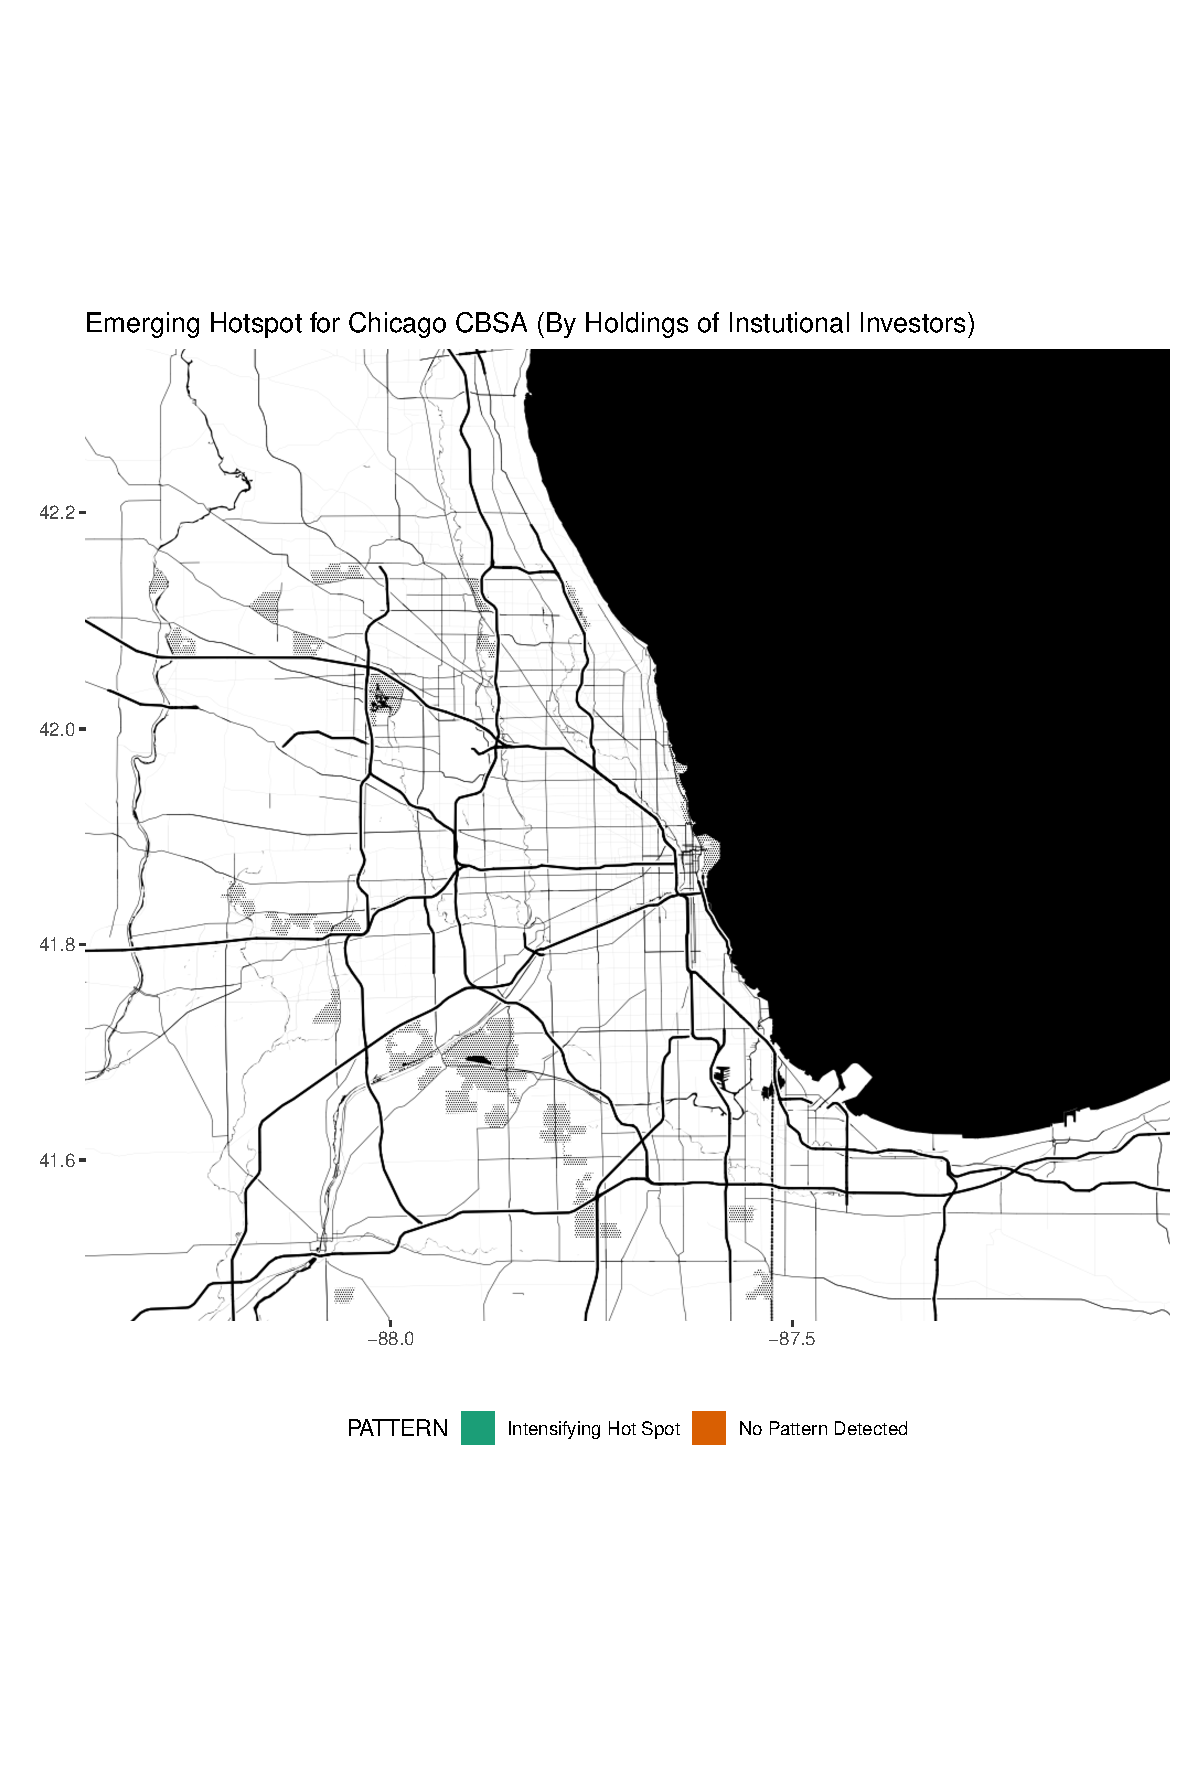
\includegraphics[width=1\linewidth]{Figures/ChapterIV/Chi_Money_EH}
	\caption[Emerging Hot Spot Analysis of Funds under Management for Chicago]{Emerging Hot Spot Analysis of Funds under Management for Chicago for period June 2013 to December 2018}
	\label{fig:Chicagonmoneyhotspot}
\end{figure}

\begin{figure}
	\centering
	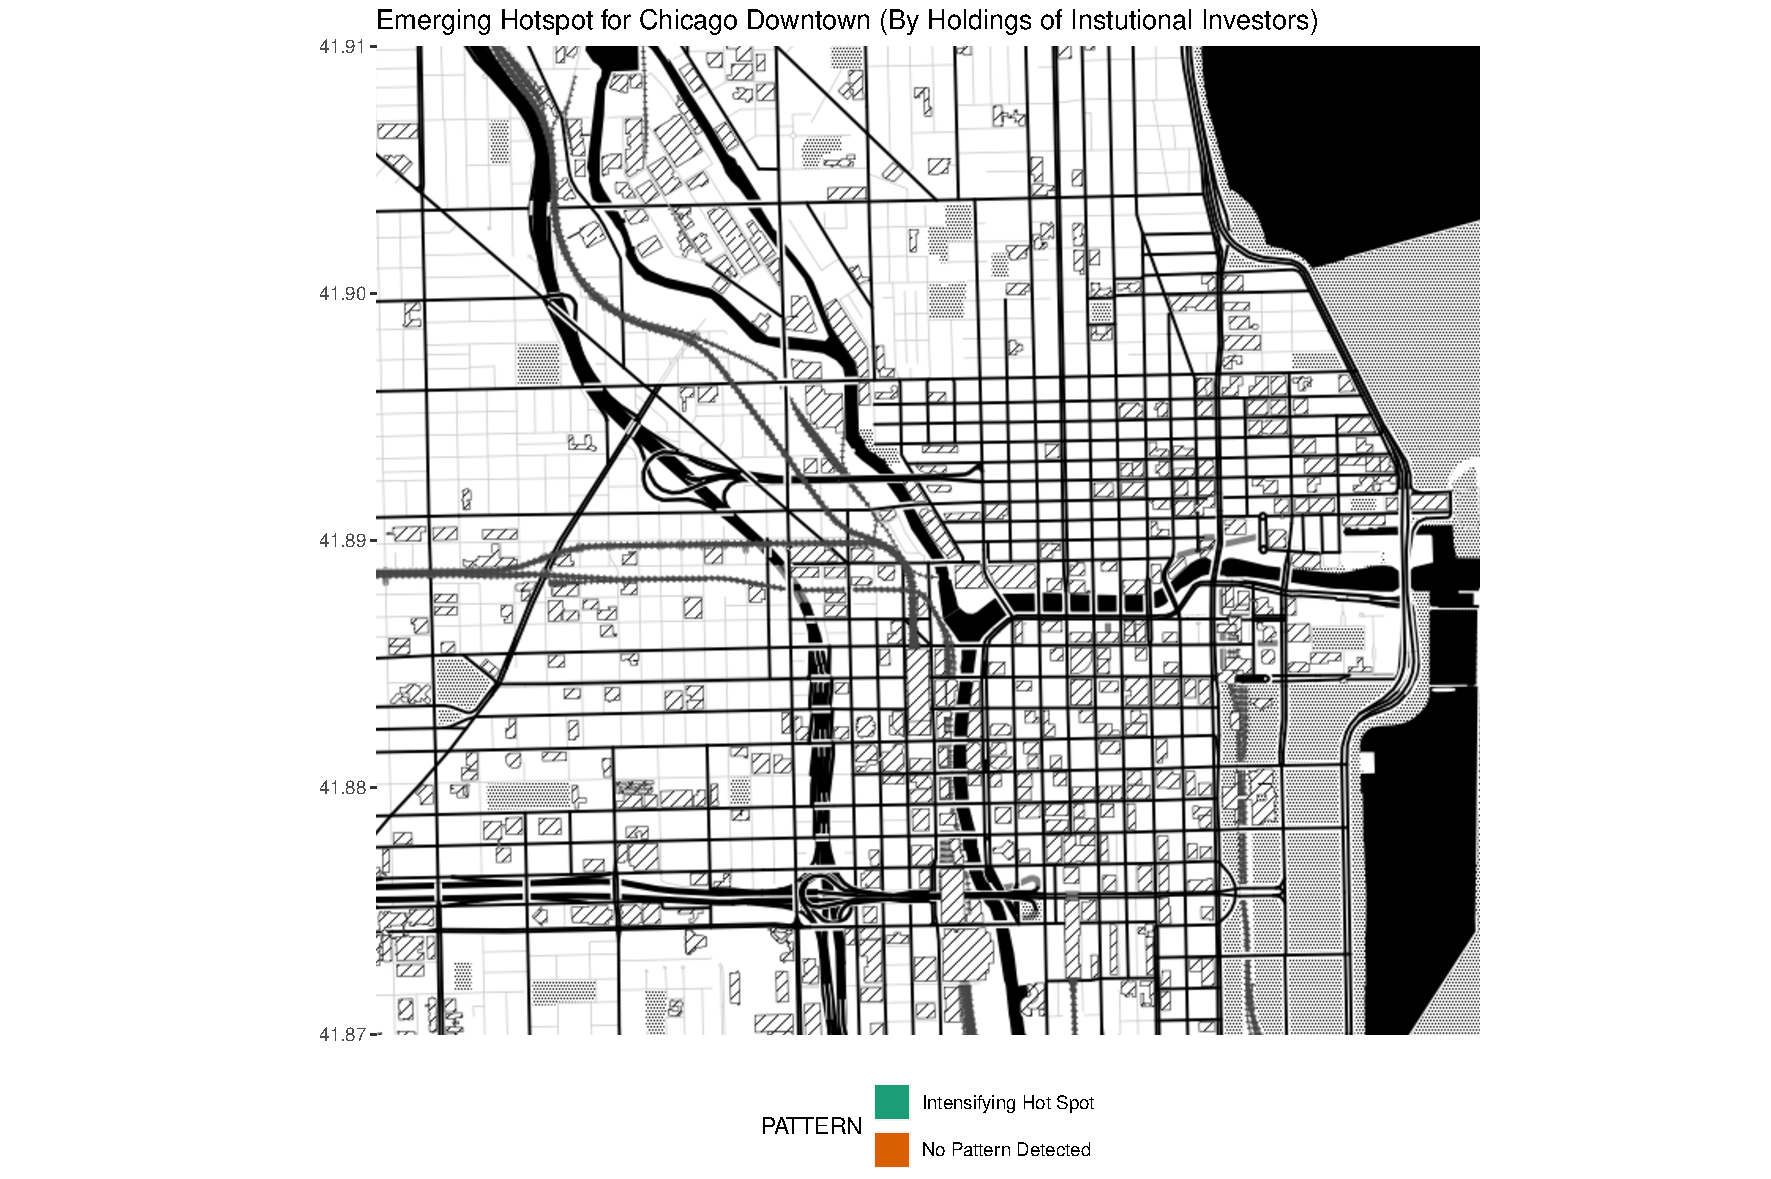
\includegraphics[width=1\linewidth]{Figures/ChapterIV/Chi_Money_EH_Downtown}
	\caption[Emerging Hot Spot Analysis of Funds under Management for Chicago]{Emerging Hot Spot Analysis of Funds under Management for Chicago for period June 2013 to December 2018}
	\label{fig:Chicagonmoneyhotspot_Downtown}
\end{figure}

Figure \ref{fig:Chicagolocaloutlier} paints a similar story than Figure \ref{fig:Chicagonmoneyhotspot}, for the main cluster of high-high hexagons is located in the Chicago Loop district.  A secondary cluster of a single high-high hexagon exists in the Napierville-Aurora region.  Furthermore, the cluster in the Loop neighbourhood of Chicago is much more defined in this analysis compared to the count map. This sharper cluster is not surprising considering the presence of the Chicago financial district, anchored by the Chicago Mercantile Exchange, at the centre of the Loop.


\begin{figure}
	\centering
	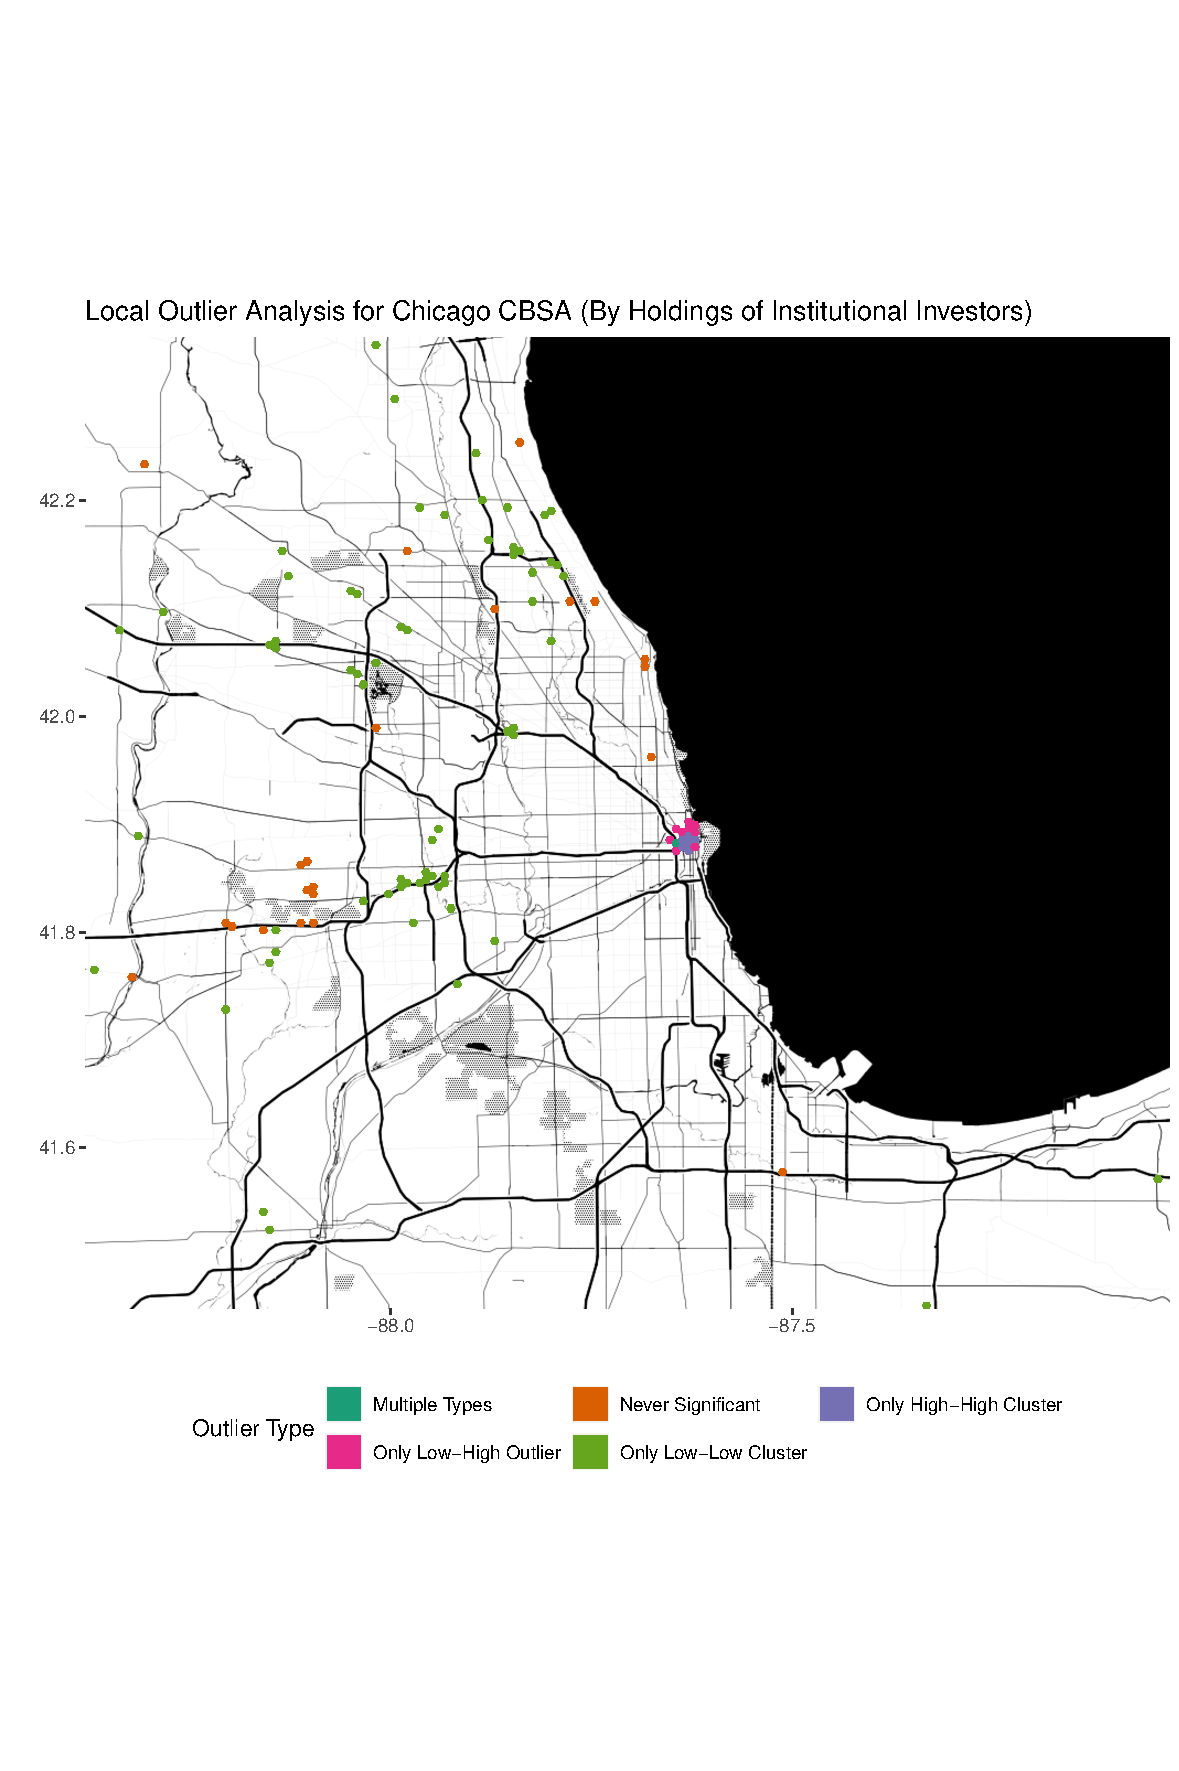
\includegraphics[width=1\linewidth]{Figures/ChapterIV/Chi_Money_LO}
	\caption[Chicago Local Outlier Analysis - Funds under Management]{Chicago Local Outlier Analysis - Funds under Management}
	\label{fig:Chicagolocaloutlier}
\end{figure}


\begin{figure}
	\centering
	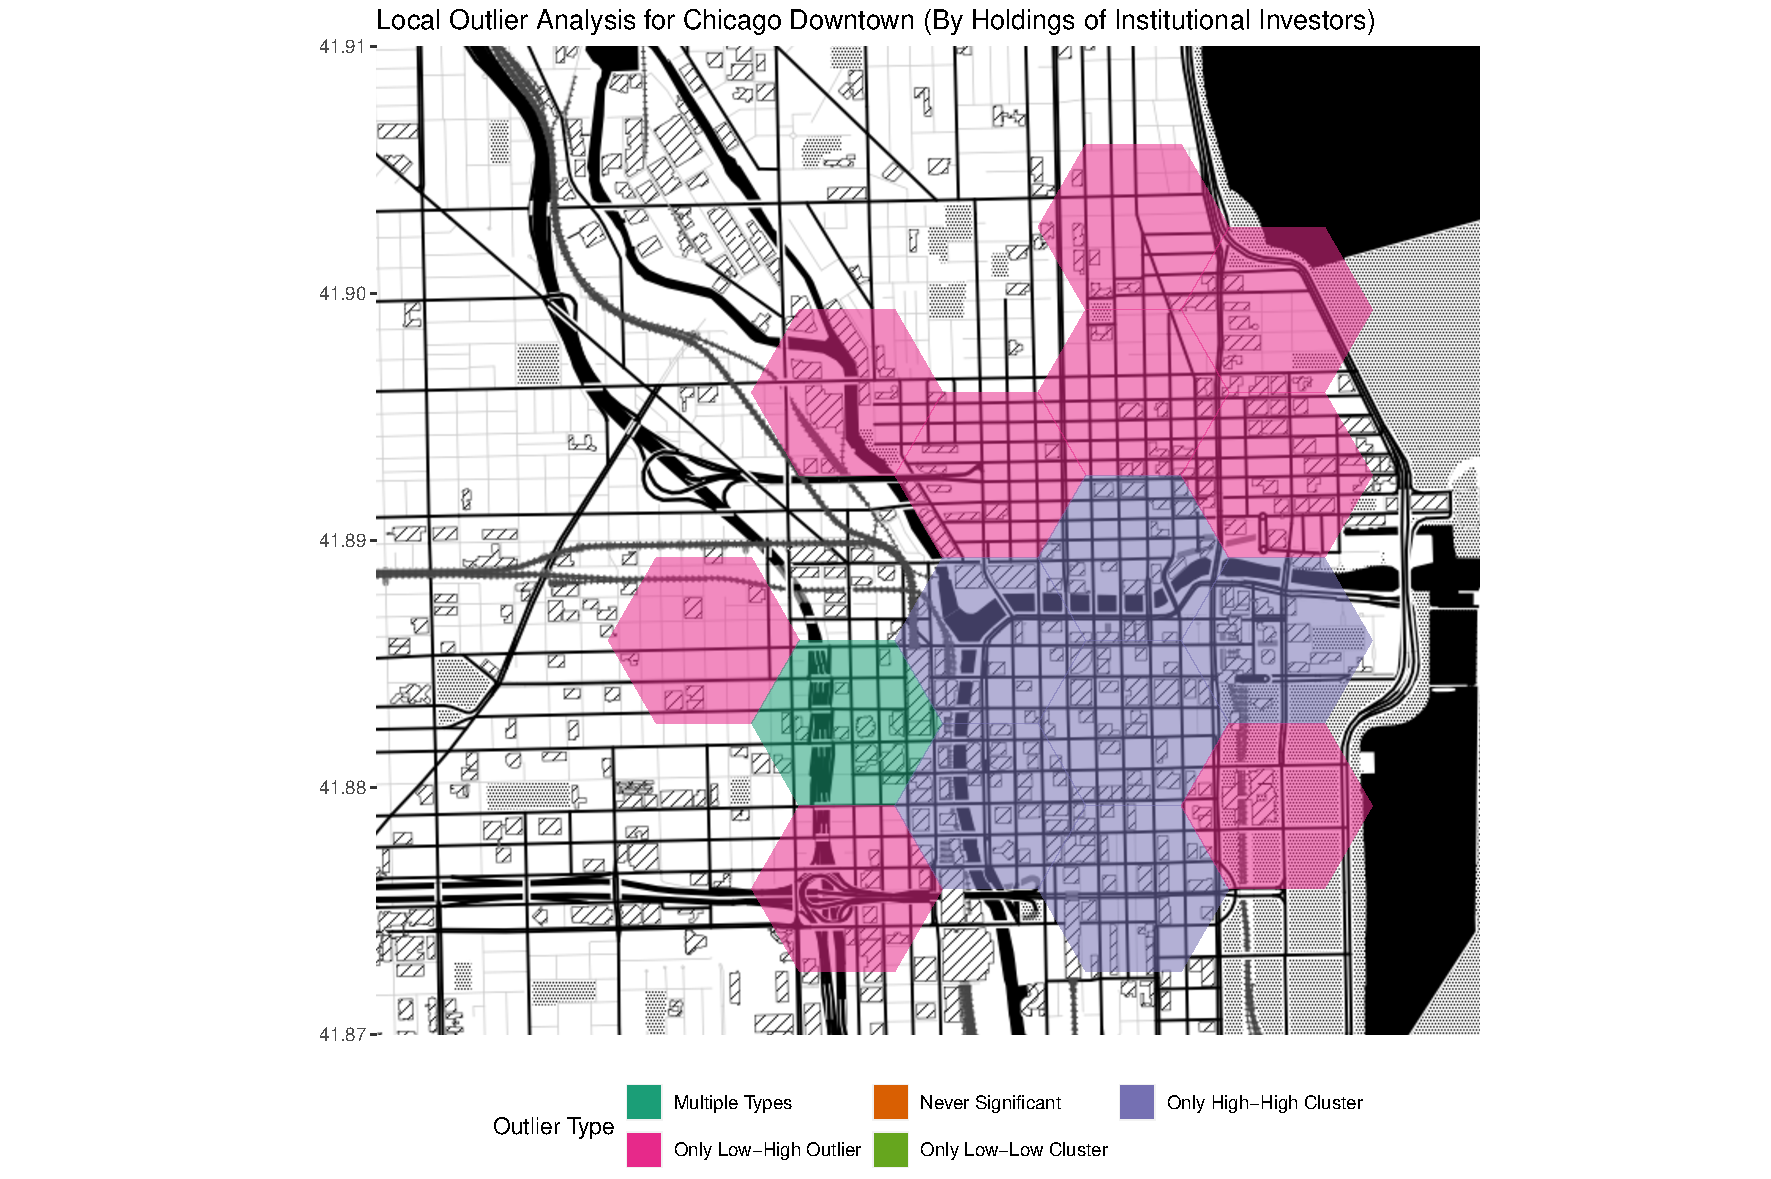
\includegraphics[width=1\linewidth]{Figures/ChapterIV/Chi_Money_LO_Downtown}
	\caption[Chicago Local Outlier Analysis - Funds under Management]{Chicago Local Outlier Analysis - Funds under Management}
	\label{fig:Chicagolocaloutlier_Downtown}
\end{figure}

\section{Los Angeles}



\subsection{Count Data}

Figure \ref{fig:LAcounthotspot} indicates that there is an absence of a central financial district and that investors are more diffused.	As such, unlike Boston and Chicago, the emerging hot spot analysis map for Los Angeles offers more categories.  This broad spread of hot spots is not really surprising considering Los Angeles's history and reputation for urban sprawl and suburban office parks \citep{dearpostmodern1998,harrisconstructing1998}.  The lack of a historic CBD comprised of skyscrapers on the scale of New York's Wall Street and Midtown or Chicago's Loop district and decentralized city administration certainly help in creating multiple small intensifying hot spots around the city such as Downtown, Santa Monica, Beverly Hills, Costa Mesa and Irvine. 

These hot spot locations also show up in Figure \ref{fig:LAcountlocaloutliercount} as local outliers.  However, there is a large amount of hexagons displaying the  mixed outlier type in Santa Monica.  This can be partially explained by the diffuse nature of locations in Santa Monica compared to other clusters such that across time they might appear as high-highs or high-lows due to neighbourhood effects.  

\begin{figure}
	\centering
	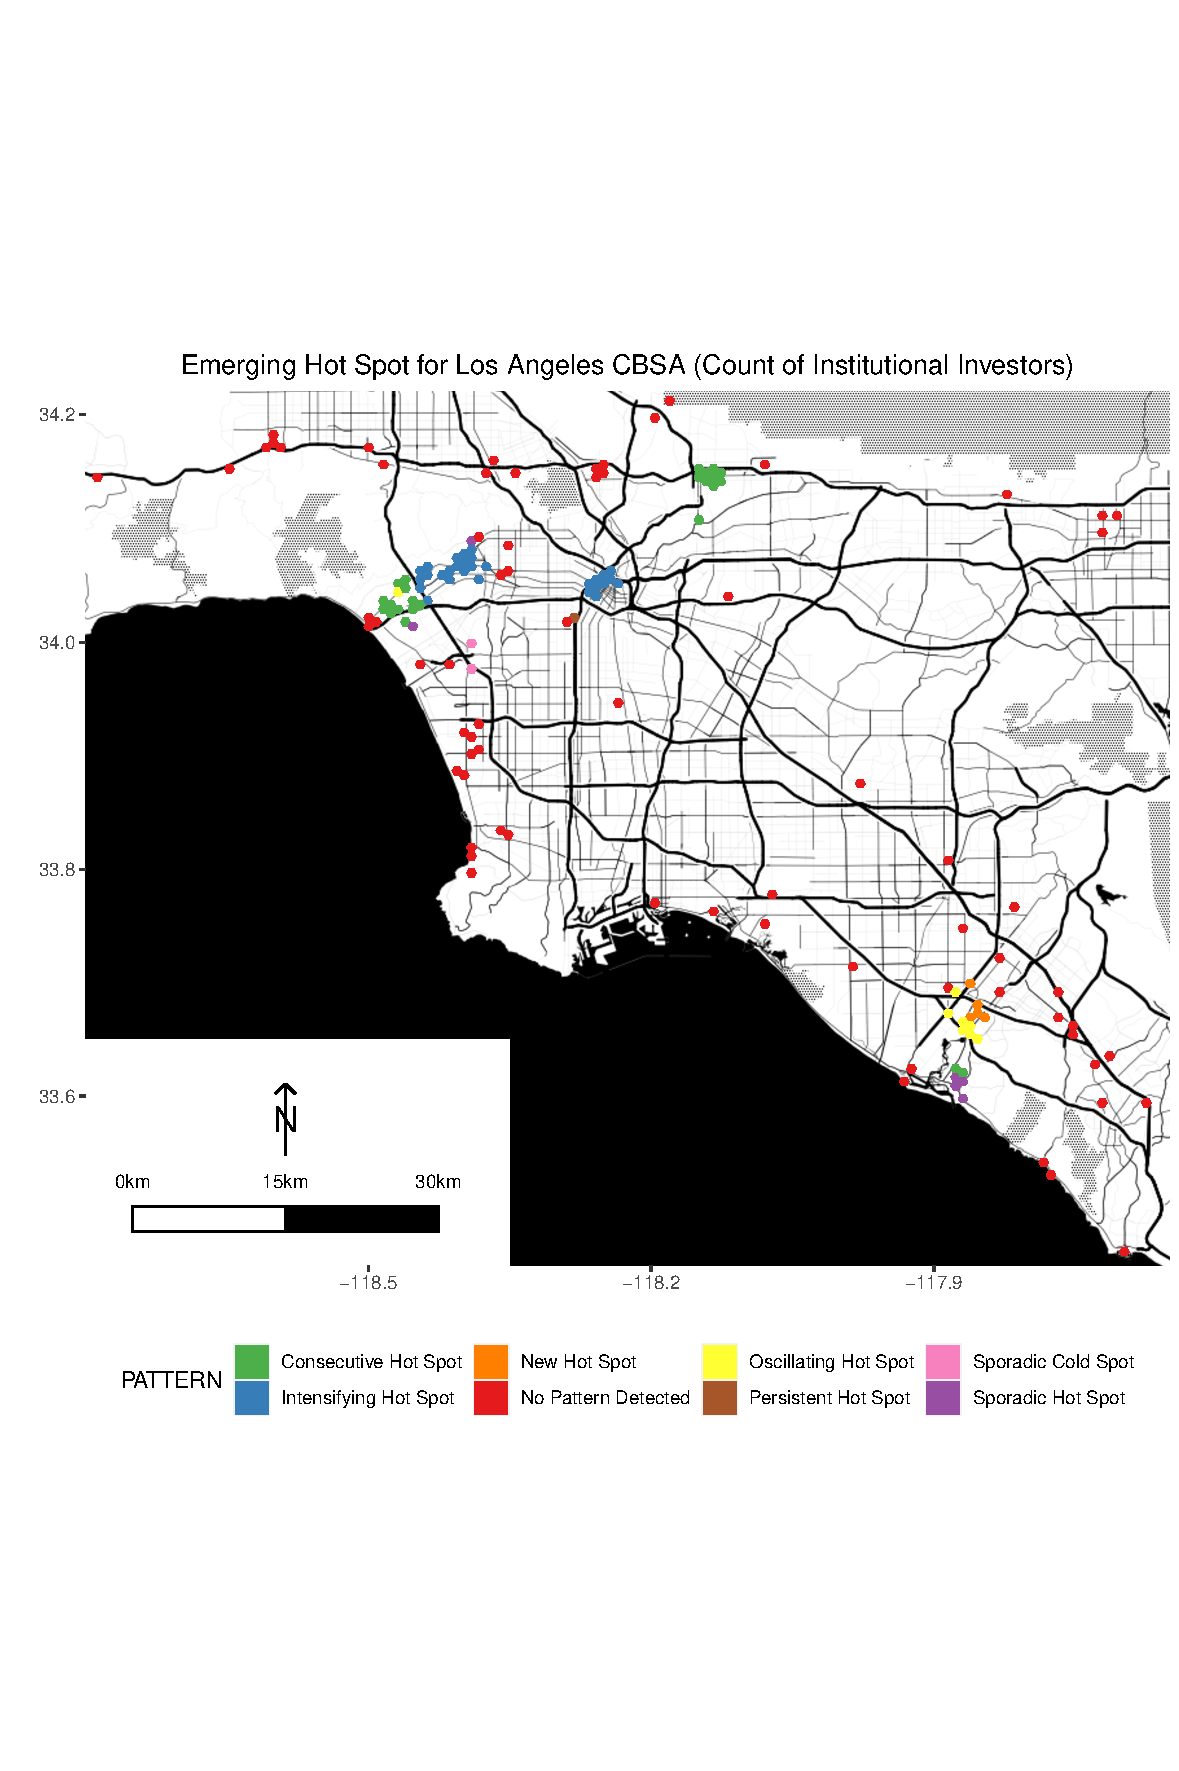
\includegraphics[width=1\linewidth]{Figures/ChapterIV/LA_Count_EH}
	\caption[Hot Spot Analysis of Number of Firms in Los Angeles]{Hot Spot Analysis of Number of Firms in Los Angeles for the time period March 1999 to December 2018}
	\label{fig:LAcounthotspot}
\end{figure}

\begin{figure}
	\centering
	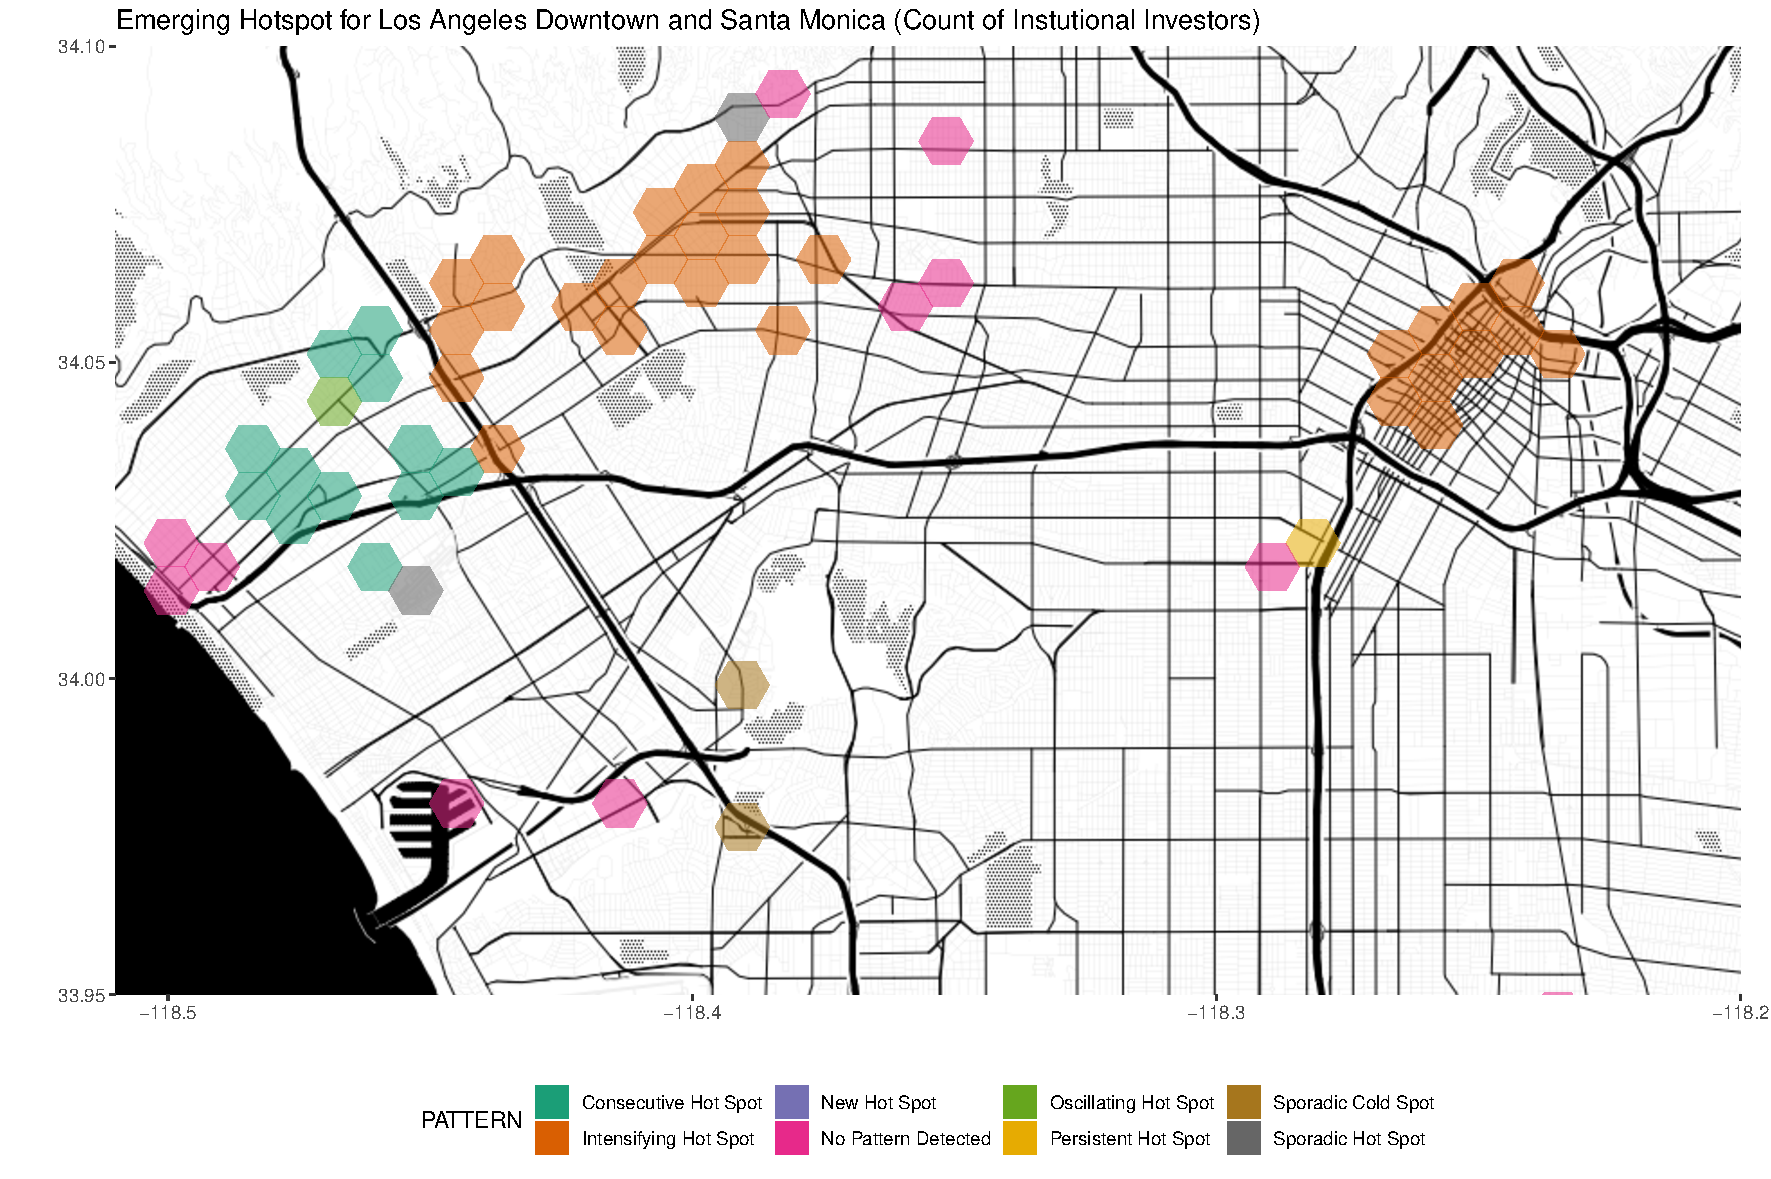
\includegraphics[width=1\linewidth]{Figures/ChapterIV/LA_Count_EH_Downtown}
	\caption[Hot Spot Analysis of Number of Firms in Downtown Los Angeles and Santa Monica]{Hot Spot Analysis of Number of Firms in Downtown Los Angeles and Santa Monica for the time period March 1999 to December 2018}
	\label{fig:LAcounthotspot_Downtown}
\end{figure}


\begin{figure}
	\centering
	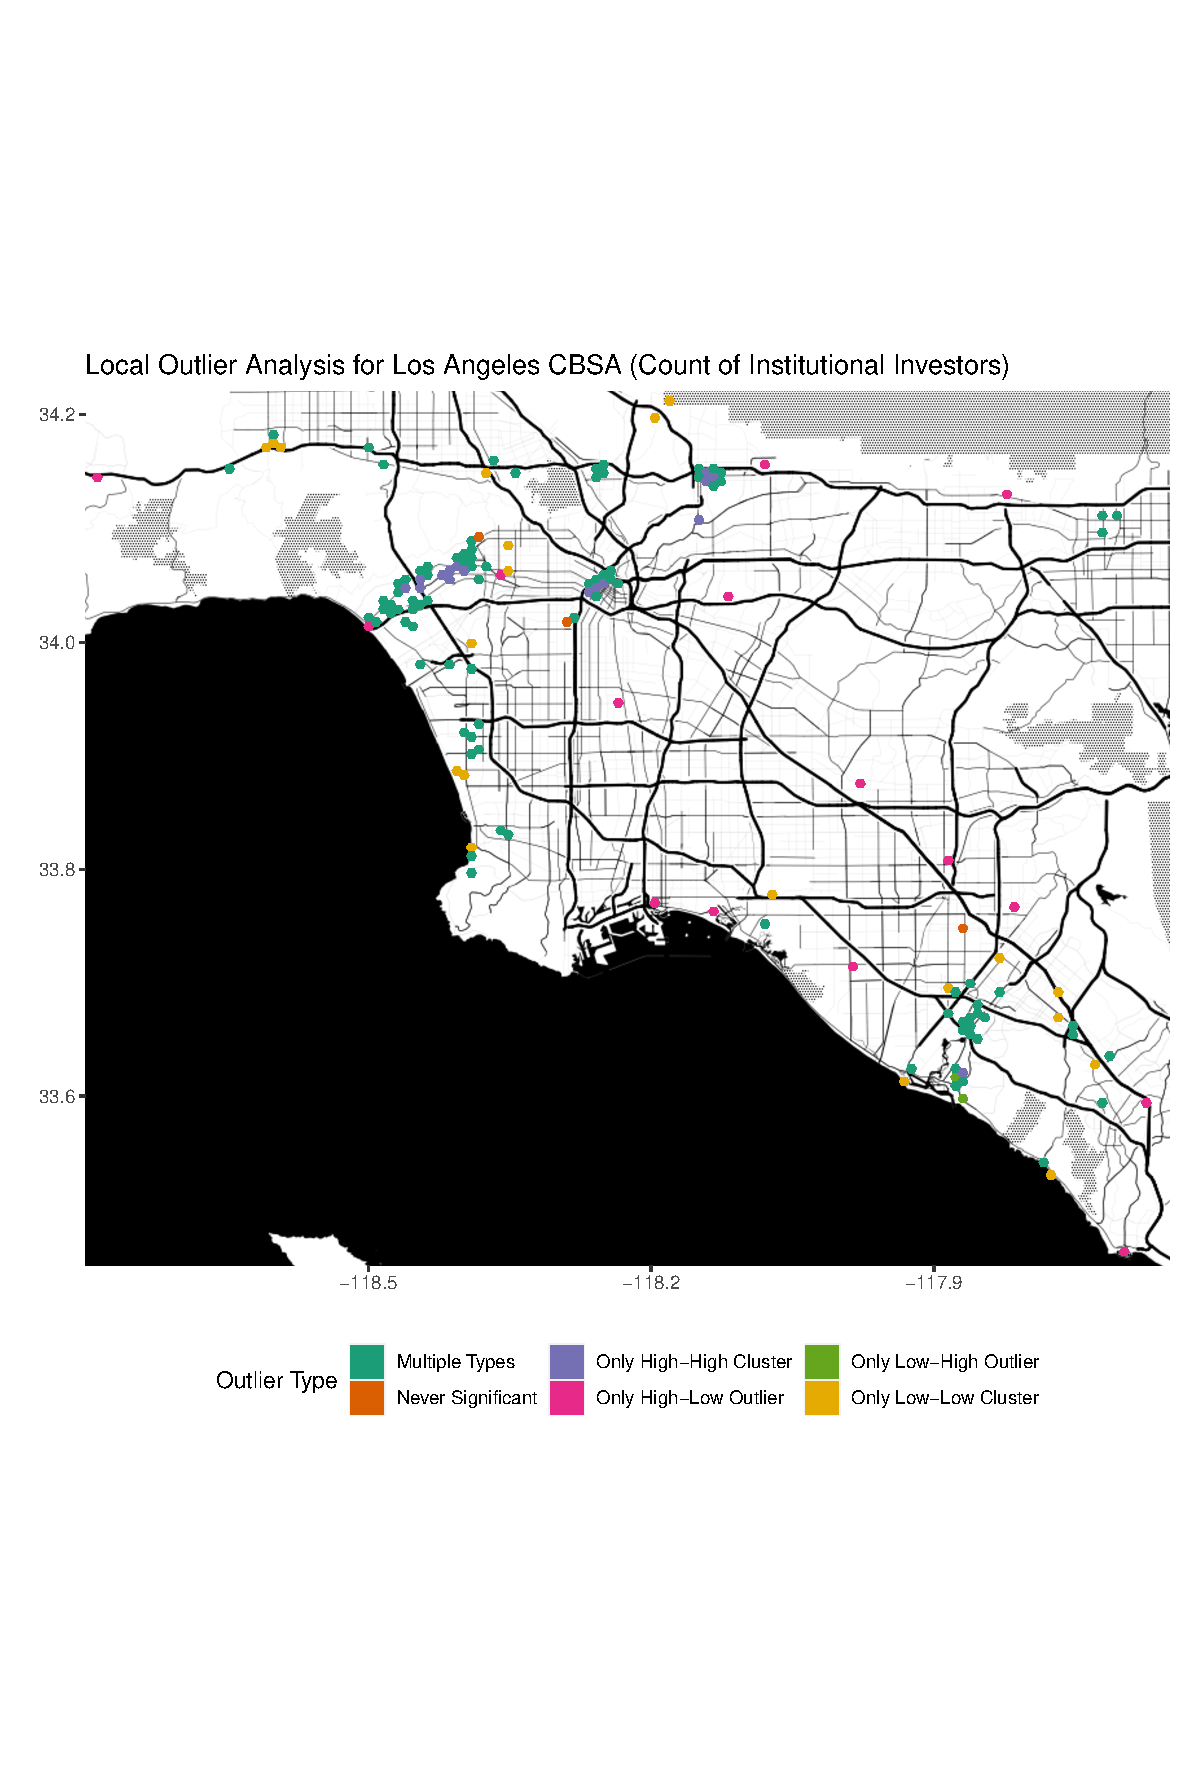
\includegraphics[width=1\linewidth]{Figures/ChapterIV/LA_Count_LO}
	\caption[Los Angeles Local Outlier Analysis - Count of Institutional Investors]{Los Angeles Local Outlier Analysis - Count of Institutional Investors}
	\label{fig:LAcountlocaloutliercount}
\end{figure}	

\begin{figure}
	\centering
	\includegraphics[width=1\linewidth]{Figures/ChapterIV/LA_Count_LO_Downtown}
	\caption[Downtown Los Angeles and Santa Monica Local Outlier Analysis - Count of Institutional Investors]{Downtown Los Angeles and Santa Monica Local Outlier Analysis - Count of Institutional Investors}
	\label{fig:LAcountlocaloutliercount_Downtown}
\end{figure}	

\subsection{Funds Under Management}

Continuing the theme seen in all previous maps with regards to analysing funds under management, the map that is weighted by money rather then the mere presence of an investor reduces the importance of suburban investors.  This suggests that while suburban investors are becoming more common, their portfolio of holdings are smaller than CBD-based investors.  

The emerging hot spot analysis for Figure \ref{fig:LAmoneyhotspot} as well as the local outlier analysis in Figure \ref{fig:LAlocaloutlier} drops the Costa Mesa  and Irvine hot spots.  Furthermore, the Downtown Los Angeles hot spot remains the only one that is still an intensifying hot spot.  This can be explained by the recent construction boom in high grade office towers being built in the Downtown after an influx of foreign capital and a planning mandate towards densification \citep{Marino19}.  


\begin{figure}
	\centering
	\includegraphics[width=1\linewidth]{Figures/ChapterIV/LA_Money_EH}
	\caption[Emerging Hot Spot Analysis of Funds under Monument for Los Angeles]{Emerging Hot Spot Analysis of Funds under Monument for Los Angeles for period June 2013 to December 2018}
	\label{fig:LAmoneyhotspot}
\end{figure}

\begin{figure}
	\centering
	\includegraphics[width=1\linewidth]{Figures/ChapterIV/LA_Money_EH_Downtown}
	\caption[Emerging Hot Spot Analysis of Funds under Monument for Downtown Los Angeles and Santa Monica]{Emerging Hot Spot Analysis of Funds under Monument for Downtown Los Angeles and Santa Monica for period June 2013 to December 2018}
	\label{fig:LAmoneyhotspot_Downtown}
\end{figure}

\begin{figure}
	\centering
	\includegraphics[width=1\linewidth]{Figures/ChapterIV/LA_Money_LO}
	\caption[Los Angeles Local Outlier Analysis - Funds under Management]{Los Angeles Local Outlier Analysis - Funds under Management}
	\label{fig:LAlocaloutlier}
\end{figure}

\begin{figure}
	\centering
	\includegraphics[width=1\linewidth]{Figures/ChapterIV/LA_Money_LO_Downtown}
	\caption[Downtown Los Angeles and Santa Monica Local Outlier Analysis - Funds under Management]{Downtown Los Angeles and Santa Monica Local Outlier Analysis - Funds under Management}
	\label{fig:LAlocaloutlier_Downtown}
\end{figure}

\section{New York City}

\subsection{Count Data}

Figure \ref{fig:NYCcounthotspot} displays the singular emerging hot spot cluster for the New York region.  Unsurprisingly, this hot spot covers the heart of the US financial universe: the Financial District and Midtown on Manhattan Island, and extending somewhat into the Bronx, Brooklyn and Hudson County, New Jersey.   Furthermore, the intensifying hotspot over Manhattan and the constant hot spot to the south of it is evidence in the shift northwards towards Midtown Manhattan due to the desire to be near the intercontinental exchange - that is to say where transatlantic fiber optic cables come to shore in North America.     

Providing more detailed spatial resolution on high-high hot spots, Figure \ref{fig:NYCcountlocaloutliercount} finds that most of the high-high hexes are located in Manhattan, and a few isolated hexes are located in Brooklyn, Bronx and Hudson Counties.  Notable by its absence, the highly residential Stuyvesant Town neighbourhood on the east side of Manhattan is largely devoid of institutional investors.      



\begin{figure}
	\centering
	\includegraphics[width=1\linewidth]{Figures/ChapterIV/NY_Count_EH}
	\caption[Hot Spot Analysis of Number of Firms in New York]{Hot Spot Analysis of Number of Firms in New York for the time period March 1999 to December 2018}
	\label{fig:NYCcounthotspot}
\end{figure}


\begin{figure}
	\centering
	\includegraphics[width=1\linewidth]{Figures/ChapterIV/NY_Count_EH_Downtown}
	\caption[Hot Spot Analysis of Number of Firms in New York]{Hot Spot Analysis of Number of Firms in New York for the time period March 1999 to December 2018}
	\label{fig:NYCcounthotspot_Downtown}
\end{figure}

\begin{figure}
	\centering
	\includegraphics[width=1\linewidth]{Figures/ChapterIV/NY_Count_LO}
	\caption[New York Local Outlier Analysis - Count of Institutional Investors]{New York Local Outlier Analysis - Count of Institutional Investors}
	\label{fig:NYCcountlocaloutliercount}
\end{figure}	

\begin{figure}
	\centering
	\includegraphics[width=1\linewidth]{Figures/ChapterIV/NY_Count_LO_Downtown}
	\caption[New York Local Outlier Analysis - Count of Institutional Investors]{New York Local Outlier Analysis - Count of Institutional Investors}
	\label{fig:NYCcountlocaloutliercount_Downtown}
\end{figure}
\subsection{Funds Under Management}

Once again, the use of funds under management as the unit of measure for emerging hot spot analysis shows a more restrictive hot spot. In fact, Figure \ref{fig:NYCmoneyhotspot} is simply a more restrictive version of Figure \ref{fig:NYCcounthotspot}.  The same can be said of Figure \ref{fig:NYClocaloutlier} treatment of local outlier analysis when compared to Figure \ref{fig:NYCcountlocaloutliercount}.  That being said, this more restrictive criteria removes most of the high-high clusters in Hudson County and Brooklyn County, suggesting once again that these investors located outside of the CBD have a smaller bankroll than the investors located in the CBD.   

\begin{figure}
	\centering
	\includegraphics[width=1\linewidth]{Figures/ChapterIV/NY_Money_EH}
	\caption[Emerging Hot Spot Analysis of Funds under Management for New York]{Emerging Hot Spot Analysis of Funds under Management for New York for period June 2013 to December 2018}
	\label{fig:NYCmoneyhotspot}
\end{figure}

\begin{figure}
	\centering
	\includegraphics[width=1\linewidth]{Figures/ChapterIV/NY_Money_EH_Downtown}
	\caption[Emerging Hot Spot Analysis of Funds under Management for New York]{Emerging Hot Spot Analysis of Funds under Management for New York for period June 2013 to December 2018}
	\label{fig:NYCmoneyhotspot_Downtown}
\end{figure}


\begin{figure}
	\centering
	\includegraphics[width=1\linewidth]{Figures/ChapterIV/NY_Money_LO}
	\caption[New York Local Outlier Analysis - Funds under Management]{New York Local Outlier Analysis - Funds under Management}
	\label{fig:NYClocaloutlier}
\end{figure}

\begin{figure}
	\centering
	\includegraphics[width=1\linewidth]{Figures/ChapterIV/NY_Money_LO_Downtown}
	\caption[New York Local Outlier Analysis - Funds under Management]{New York Local Outlier Analysis - Funds under Management}
	\label{fig:NYClocaloutlier_Downtown}
\end{figure}


\section{San Francisco}


\subsection{Count Data}

Figure \ref{fig:SFcounthotspot} displays five hot spots: an emerging hot spot in San Francisco's central business district, San Mateo, a small emerging centre north of the Golden Gate Bridge along with consecutive hot spots in Palo Alto and Walnut Creek.   

\begin{figure}
	\centering
	\includegraphics[width=1\linewidth]{Figures/ChapterIV/SF_Count_EH}
	\caption[Hot Spot Analysis of Number of Firms in San Francisco]{Hot Spot Analysis of Number of Firms in San Francisco for the time period March 1999 to December 2018}
	\label{fig:SFcounthotspot}
\end{figure}

\begin{figure}
	\centering
	\includegraphics[width=1\linewidth]{Figures/ChapterIV/SF_Count_EH_Downtown}
	\caption[Hot Spot Analysis of Number of Firms in San Francisco]{Hot Spot Analysis of Number of Firms in San Francisco for the time period March 1999 to December 2018}
	\label{fig:SFcounthotspot_Downtown}
\end{figure}

Figure \ref{fig:SFcountlocaloutliercount} displays the results of the local outlier analysis and finds the same five clusters.     

\begin{figure}
	\centering
	\includegraphics[width=1\linewidth]{Figures/ChapterIV/SF_Count_LO}
	\caption[San Francisco Local Outlier Analysis - Count of Institutional Investors]{San Francisco Local Outlier Analysis - Count of Institutional Investors}
	\label{fig:SFcountlocaloutliercount}
\end{figure}

\begin{figure}
	\centering
	\includegraphics[width=1\linewidth]{Figures/ChapterIV/SF_Count_LO_Downtown}
	\caption[San Francisco Local Outlier Analysis - Count of Institutional Investors]{San Francisco Local Outlier Analysis - Count of Institutional Investors}
	\label{fig:SFcountlocaloutliercount_Downtown}
\end{figure}

\subsection{Funds Under Management}

In a continuing theme of having the funds under management Figures \ref{fig:SFnmoneyhotspot} and \ref{fig:SFlocaloutlier} show fewer hot spots than count data.  These hot spots are located in San Francisco's CBD and in San Mateo.  	

\begin{figure}
	\centering
	\includegraphics[width=1\linewidth]{Figures/ChapterIV/SF_Money_EH}
	\caption[Emerging Hot Spot Analysis of Funds under Management for San Francisco]{Emerging Hot Spot Analysis of Funds under Management for San Francisco for period June 2013 to December 2018}
	\label{fig:SFnmoneyhotspot}
\end{figure}

\begin{figure}
	\centering
	\includegraphics[width=1\linewidth]{Figures/ChapterIV/SF_Money_EH_Downtown}
	\caption[Emerging Hot Spot Analysis of Funds under Management for San Francisco]{Emerging Hot Spot Analysis of Funds under Management for San Francisco for period June 2013 to December 2018}
	\label{fig:SFnmoneyhotspot_Downtown}
\end{figure}


\begin{figure}
	\centering
	\includegraphics[width=1\linewidth]{Figures/ChapterIV/SF_Money_LO}
	\caption[San Francisco Local Outlier Analysis - Funds under Management]{San Francisco Local Outlier Analysis - Funds under Management}
	\label{fig:SFlocaloutlier}
\end{figure}

\begin{figure}
	\centering
	\includegraphics[width=1\linewidth]{Figures/ChapterIV/SF_Money_LO_Downtown}
	\caption[San Francisco Local Outlier Analysis - Funds under Management]{San Francisco Local Outlier Analysis - Funds under Management}
	\label{fig:SFlocaloutlier_Downtown}
\end{figure}
\section{Conclusion}	


When looking at the Continental United States, it appears that institutional investors are not evenly distributed across its vast surface.  As a matter of fact, other than a few outlying homesteads of institutional investors located in State capitals, most of the investors are located in the major metro areas of Boston, Chicago, Los Angeles, New York and San Francisco.  While one might be tempted to think that this is merely a collection of large US metro areas, the absence of population rich regions such as Dallas-Fort Worth, Houston, Philadelphia, Washington DC, Miami and Atlanta from the ranks of top cities is reassuring that the top 5 cities isn't simply a replication of XKCD Comic 1138 (Figure \ref{fig:heatmapxkcd}) using institutional investors rather than subscribers to Martha Stewart. 

Across these five cities, institutional investors exhibit a strong propensity to cluster, and more often than not these clusters are located in the downtown cores of cities.  Even with Los Angeles lack of a highly developed CBD for a city of it's size, its sprawling nature and deliberately decentralized history, the  existence of investor clusters somewhat pushes back against Graves's assertion that the benefits of co-location in an urban core were more than offset by the ever increasing cost of rents, and that investors of the future might seek more peripheral locations \citep{Graves2003}.   

That being said, one should not forget that identifying clusters can be problematic.  It is possible that new firms showing up on the periphery of a metro area's suburbia might not have the required density to show up a cluster, even as the total ratio between CBD and suburbs may tilt evermore into the suburban office park's favour.  This is probably the most likely explanation for reconciling this chapter with Chapter \ref{ChapterIIIb}.  There are some hints at suburban centres being centres of clustering, notably the Route 128 in Boston, Evenston and Highland Park in Chicago, Irvine CA, and Walnut Creek in San Francisco.  However, it should be noted that these areas have a historically smaller bankroll than the investors that tend to aggregate into CBD, suggesting that there might be a size threshold where being in the CBD becomes more worthwhile than in suburban office parks.  

The buyer's remorse over choosing low land costs over a central location can been seen in the saga of the Swiss bank UBS.  This Swiss-headquartered multinational bank was attracted by Stamford Connecticut's low land prices and generous tax incentives.  However, this out of the way location became a severe hindrance in attracting top tier talent from New York's financial sector due to long commutes, as well as chronic difficulties in meeting with Manhattan-based clients \citep{NYT_2011}.    

		\chapter{LDA of Investments in the United States} 
\section{Introduction}
\nocite{tmpackage} \nocite{LDAvis} \nocite{Stargazer}
\nomenclature{MPT}{Modern Portfolio Theory}	

While chapter \ref{chapterIV} explored the locational preferences of institutional investors in the US as a whole and in the five largest American metropolitan areas by total funds under management, this chapter will explore whether geography can play a role in individual investors portfolio choices.   

While Modern Portfolio Theory (MPT), as established by \cite{Markowitz1952} advocates for holding a broad and negatively correlated portfolio, the notion of "not putting all of one's eggs in a single basket" is an old one, for \cite{Lofthouse53} finds that such advice was formally practised by the British investment firm Investment Registry as far back as 1904.  

In concert with MPT's emphasis on diversification, the reaction to the Crash of October 1987 placed renewed emphasis on risk management and the rise of ``Value at Risk'' (VAR) based investing in which firms would try to maximise returns while minimizing risk.  This led to a homogenizing effect in investment strategies, as explained by Andrew G. Haldane, executive director of the Financial Stability at the Bank of England at a conference on risk management:

\nomenclature{VAR}{Value at Risk}
\begin{quote}
	Within the financial sector, diversity appears to have been reduced for two separate, but related, reasons:  the pursuit of return;  and the management of risk.  The pursuit of yield resulted in a return on equity race among all types of financial firm.  As they collectively migrated to high-yield activities, business strategies came to be replicated across the financial sector.  Imitation became the sincerest form of flattery.
	
	So savings cooperatives transformed themselves into private commercial banks.  Commercial banks ventured into investment banking.  Investment banks developed in-house hedge funds through large proprietary trading desks.  Funds of hedge funds competed with traditional investment funds.  And investment funds - pension, money market mutual, insurance - imported the risk the others were shedding.   \citep{Haldane2009}[p.18]
\end{quote} 

As explored in Chapter \ref{ChapterII}, there is a substantial literature showing that stock pickers are biased towards industries in which they are knowledgeable or have personal connections.  In particular, \cite{covalthe2001} find that investors can draw abnormally high returns from local knowledge, and another study by \cite{Cohen2008} makes a compelling case that stock pickers are biased towards selecting stocks of companies that their board of directors contain shared alumni networks.  

Rather than looking at geographic differences of investors based on the type of institution they belong to such as but not limited to banks, hedge funds, pension funds, and insurance companies, this study will attempt to create a functional portfolio archetypes using machine learning and aggregate these archetypes by geography in order to look for regional patterns.   

\section{Latent Dirichlet allocation}

\nomenclature{LDA}{Latent Dirichlet allocation}

Latent Dirichlet allocation (LDA) \nomenclature{LDA}{Latent Dirichlet allocation} is a generative statistical technique developed by David Blei to find themes that are common across a corpus of texts \citep{blei2003latent}.  This technique is a derivation and refinement of \cite{Papadimitriou98} and \cite{PAPADIMITRIOU2000217} work on Latent Semantic Indexing.  

LDA has made certain classification tasks feasible to conduct in a short time, such as analysing a large sample of digitized 18th century American newspapers for the topics of the day that would otherwise be unfeasible for any individual to read \citep{newman2006probabilistic}.  Another well known use of LDA is for finding in near-realtime the topics of controversy and/or debate at an academic conference via Twitter usage by the participants of the conference \citep{Marwick2013}.

In addition to text analysis, LDA has been used in multiple different fields such as finding latent patterns in biodiversity data \citep{Vale2014}, genetic data, images, social networks \citep{Blei2012} as well as remote sensing data \cite{Lienou2010}.

\subsection{How does LDA work?}

Ted Underwood, who studies the intersection of Information Science and English Literature, contends in his academic blog post entitled ``Topic modeling made just simple enough[sic]" that academic papers make LDA look much harder than it is in practice, since their main goal is to show how and why their underlying formulas work and the mathematical proofs rely on highly advanced mathematics. If we take the algorithms to work as intended, the practice of LDA can be easily explained in practice \citep{Underwood2012}.

LDA assumes that each document being analyzed contains a multitude of different topics, and each of these topics are latent, that is to say they can't be directly observed, but can be defined indirectly. Edwin Chen's classic introduction to LDA example is quite straight forward \citep{Chen2011}.  Take the following five sentences:

\begin{enumerate}
	\singlespacing 
	\item I like to eat broccoli and bananas.
	\item I ate a banana and spinach smoothie for breakfast.
	\item Chinchillas and kittens are cute.
	\item My sister adopted a kitten yesterday.
	\item Look at this cute hamster munching on a piece of broccoli.
\end{enumerate}

If we treat each sentence as a document for LDA purposes, and we were to limit ourselves to two topics, we would see something to the effect of the following:

\begin{itemize}
	\item \textbf{Sentences 1 and 2:} 100\% Topic A
	\item \textbf{Sentences 3 and 4:} 100\% Topic B
	\item \textbf{Sentence 5:} 60\% Topic A, 40\% Topic B
\end{itemize}

At this point, we see that the topics consists of:
\begin{itemize}	
	\item \textbf{Topic A:} 30\% broccoli, 15\% bananas, 10\% breakfast, 10\% munching, etc... 
	
	\item \textbf{Topic B:} 20\% chinchillas, 20\% kittens, 20\% cute, 15\% hamster, etc...  
\end{itemize}

At which point, we can see that Topic A consists mostly of food and food adjacent activities, whereas Topic B is about animals and their general cuteness. 

At this point, it is important to state that LDA assumes that language is a "bag of words". That is to say that for the purpose of the model, the order of words and punctuation isn't considered important information.  While this may cause some miss-coding of information in a limited context, since grammar, punctuation and word order can relay important information, larger corpora smooth-out these ambiguities. For example, an LDA model would treat the following two sentences as being identical:

\begin{itemize}	
	\item  Have you eaten, my child?
	
	\item  Have you eaten my child\textinterrobang 
\end{itemize}

This study will be using LDA on Stock unique identifiers (CUSIP), the "bag of words" methodology works to our advantage, since the presented order of stocks in an institutional investor's portfolio will not influence the sorting algorithm. This relative location agnosticism is useful in this case, since unlike earth movers' distance classification \citep{rubner2000earth}, this method of classification is dependant on the initial relative distribution within the input variables, and therefore there is no need for a special ordering of stock positions in the input file.  


The LDA process is mapped out graphically in Figure \ref{fig:LDA_graphic} and written out in Equation \ref{LDAequation}. For each possible topic (Z), 


\begin{equation}
P(Z|W,D) = \dfrac{\# \text{ of words } W \text{ in topic } Z + \beta_{w}}{\text{total tokens in } Z + \beta}*(\# \text{ of words in } D \text{ that belong to } Z + \alpha)
\label{LDAequation}
\end{equation}



\begin{figure}[H]
	\tikzset{every picture/.style={line width=0.75pt}} %set default line width to 0.75pt        
	
	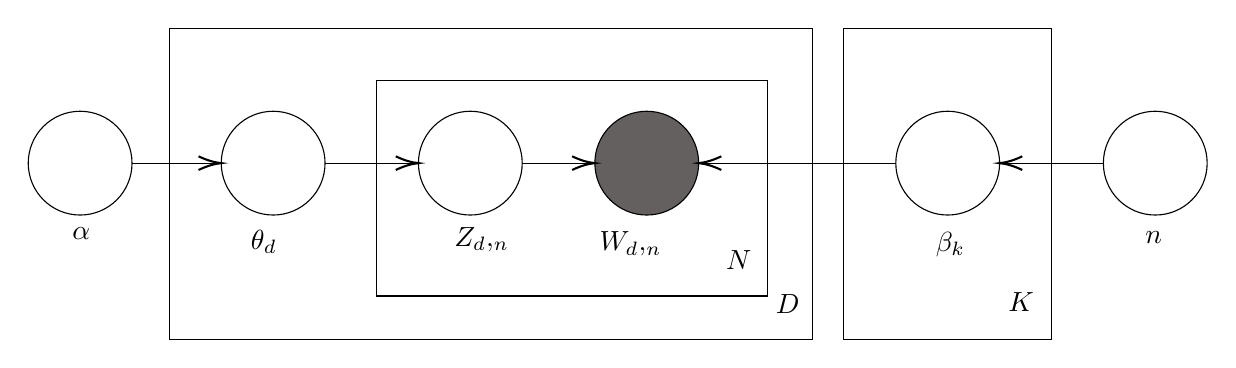
\begin{tikzpicture}[x=0.75pt,y=0.75pt,yscale=-1,xscale=1]
	%uncomment if require: \path (0,179); %set diagram left start at 0, and has height of 179
	
	%Shape: Rectangle [id:dp21726410884148195] 
	\draw   (235,38) -- (423,38) -- (423,142) -- (235,142) -- cycle ;
	%Shape: Rectangle [id:dp8470156804479287] 
	\draw   (135,13) -- (445,13) -- (445,163) -- (135,163) -- cycle ;
	%Shape: Rectangle [id:dp5437180445728402] 
	\draw   (460,13) -- (560,13) -- (560,163) -- (460,163) -- cycle ;
	%Shape: Circle [id:dp6027361372166333] 
	\draw   (67,78) .. controls (67,64.19) and (78.19,53) .. (92,53) .. controls (105.81,53) and (117,64.19) .. (117,78) .. controls (117,91.81) and (105.81,103) .. (92,103) .. controls (78.19,103) and (67,91.81) .. (67,78) -- cycle ;
	%Shape: Circle [id:dp5441473658198903] 
	\draw   (160,78) .. controls (160,64.19) and (171.19,53) .. (185,53) .. controls (198.81,53) and (210,64.19) .. (210,78) .. controls (210,91.81) and (198.81,103) .. (185,103) .. controls (171.19,103) and (160,91.81) .. (160,78) -- cycle ;
	%Shape: Circle [id:dp028671426160656655] 
	\draw   (255,78) .. controls (255,64.19) and (266.19,53) .. (280,53) .. controls (293.81,53) and (305,64.19) .. (305,78) .. controls (305,91.81) and (293.81,103) .. (280,103) .. controls (266.19,103) and (255,91.81) .. (255,78) -- cycle ;
	%Shape: Circle [id:dp6901716019104538] 
	\draw  [fill={rgb, 255:red, 101; green, 96; blue, 96 }  ,fill opacity=1 ] (340,78) .. controls (340,64.19) and (351.19,53) .. (365,53) .. controls (378.81,53) and (390,64.19) .. (390,78) .. controls (390,91.81) and (378.81,103) .. (365,103) .. controls (351.19,103) and (340,91.81) .. (340,78) -- cycle ;
	%Shape: Circle [id:dp7815059339533368] 
	\draw   (485,78) .. controls (485,64.19) and (496.19,53) .. (510,53) .. controls (523.81,53) and (535,64.19) .. (535,78) .. controls (535,91.81) and (523.81,103) .. (510,103) .. controls (496.19,103) and (485,91.81) .. (485,78) -- cycle ;
	%Shape: Circle [id:dp45137687393472814] 
	\draw   (585,78) .. controls (585,64.19) and (596.19,53) .. (610,53) .. controls (623.81,53) and (635,64.19) .. (635,78) .. controls (635,91.81) and (623.81,103) .. (610,103) .. controls (596.19,103) and (585,91.81) .. (585,78) -- cycle ;
	%Straight Lines [id:da3313227430829817] 
	\draw    (117,78) -- (158,78) ;
	\draw [shift={(160,78)}, rotate = 180] [color={rgb, 255:red, 0; green, 0; blue, 0 }  ][line width=0.75]    (10.93,-3.29) .. controls (6.95,-1.4) and (3.31,-0.3) .. (0,0) .. controls (3.31,0.3) and (6.95,1.4) .. (10.93,3.29)   ;
	%Straight Lines [id:da2686493807462953] 
	\draw    (210,78) -- (253,78) ;
	\draw [shift={(255,78)}, rotate = 180] [color={rgb, 255:red, 0; green, 0; blue, 0 }  ][line width=0.75]    (10.93,-3.29) .. controls (6.95,-1.4) and (3.31,-0.3) .. (0,0) .. controls (3.31,0.3) and (6.95,1.4) .. (10.93,3.29)   ;
	%Straight Lines [id:da5780607817492671] 
	\draw    (305,78) -- (338,78) ;
	\draw [shift={(340,78)}, rotate = 180] [color={rgb, 255:red, 0; green, 0; blue, 0 }  ][line width=0.75]    (10.93,-3.29) .. controls (6.95,-1.4) and (3.31,-0.3) .. (0,0) .. controls (3.31,0.3) and (6.95,1.4) .. (10.93,3.29)   ;
	%Straight Lines [id:da026847412265174286] 
	\draw    (485,78) -- (392,78) ;
	\draw [shift={(390,78)}, rotate = 360] [color={rgb, 255:red, 0; green, 0; blue, 0 }  ][line width=0.75]    (10.93,-3.29) .. controls (6.95,-1.4) and (3.31,-0.3) .. (0,0) .. controls (3.31,0.3) and (6.95,1.4) .. (10.93,3.29)   ;
	%Straight Lines [id:da15128656608765012] 
	\draw    (585,78) -- (537,78) ;
	\draw [shift={(535,78)}, rotate = 360] [color={rgb, 255:red, 0; green, 0; blue, 0 }  ][line width=0.75]    (10.93,-3.29) .. controls (6.95,-1.4) and (3.31,-0.3) .. (0,0) .. controls (3.31,0.3) and (6.95,1.4) .. (10.93,3.29)   ;
	
	% Text Node
	\draw (87,107.9) node [anchor=north west][inner sep=0.75pt]    {$\alpha $};
	% Text Node
	\draw (173,108.9) node [anchor=north west][inner sep=0.75pt]    {$\theta _{d}$};
	% Text Node
	\draw (271,107.9) node [anchor=north west][inner sep=0.75pt]    {$Z_{d} ,_{n}$};
	% Text Node
	\draw (402,118.9) node [anchor=north west][inner sep=0.75pt]    {$N$};
	% Text Node
	\draw (341,109.9) node [anchor=north west][inner sep=0.75pt]    {$W_{d},_{n}$};
	% Text Node
	\draw (426,139.9) node [anchor=north west][inner sep=0.75pt]    {$D$};
	% Text Node
	\draw (503,109.9) node [anchor=north west][inner sep=0.75pt]    {$ \beta_{k}$};
	% Text Node
	\draw (538,138.9) node [anchor=north west][inner sep=0.75pt]    {$K$};
	% Text Node
	\draw (604,109.9) node [anchor=north west][inner sep=0.75pt]    {$n$};
	
	
	\end{tikzpicture}
	\caption[Graphical Model of Latent Dirichlet allocation]{Graphical Model of Latent Dirichlet allocation replicated from the graphic in Blei (2012), where K is the total number of topics, $ \beta _{k}$ is the topic, a distribution over the vocabulary, $D$ is the total number of documents, $\Theta_{d}$ is the per-document topic proportions, N is the total number of words in a document, $Z_{d},_{n}$ is the per-word topic assignment, $W_{d},_{n}$ observed word, and finally $\alpha$ and $n$ as dirichlet parameters. }
	
	\label{fig:LDA_graphic}
\end{figure}



\section{Preparing the Data}
A closer analogue to using LDA is using this technique to classifying card selection in games such as Magic:The Gathering \citep{Hlynsson2017}.  This collectible card game uses 60 cards decks that are selected ahead of time by the player.  Due the game's complex resource system and multiple different strategies for attacking one's opponent, cards are not fungible, and thus the game consolidates towards certain discreet collection of cards.  Similarly, the use LDA can be used to aggregate different stock portfolios into different investment strategies strategies.  

In order to conduct an LDA analysis, the data was taken from the XBRL database of 13-F HR database for the period of the second quarter of 2013 to the end of 2018.  The process used in collecting and cleaning this data was explained in Chapter \ref{Section:13F}.  

Unfortunately the database had to be pruned of all holdings of less than 1 million dollars so that the matrix operations conducted by the LDA package would fit within the computer's available RAM (Random Access Memory).  At the time, these computers contained 32gb of RAM. This value of 1 million dollars was achieved in an iterative manner, with one computer starting with all transactions above 10 million dollars and reducing this threshold by 1 million dollars every time the LDA converged on a solution and a second computer starting with all transactions and pruning by increments of 100 000 USD until the algorithm converged rather than crash the program due to overwhelming the available RAM.  Furthermore, due to the nature of the LDA algorithm (needing full matrix operations), it was unfeasible to spread the workload across multiple computers, nor to slice the program into year-long slices and perform 5 LDA analyses, since this would give us the worst of both worlds - no time continuity, and the multiple testing problem. 

In practice, this reduces the size of the database from X to Y filers, and the value Xhat to Yhat.  That being said, the pruning of the database focuses the analysis on stock positions that have substantial, if theoretical, corporate power
%\footnote{Such as but not limited to voting rights and the threat of lowering stock prices in a mass sell-off being the best alternative to a negotiated solution.} 
rather than holdings that are simply intended passively to accrue in value and render dividends as part of a diversification strategy under the modern portfolio theory.

Furthermore, in this LDA analysis each filer-quarter is treated as independent filers in the LDA model. Stock positions do shift over time to the point that acting on information 45 days old can be ruinous, a fact that many whale watchers repeat in their newsletters and news reports \citep{Whale_Watching_CNBC_12,cramerwhale}. Since stock positions shift over time to newer strategies, this should not pose a problem; for example this would treat a caterpillar and a butterfly differently.  While indubitably the same creature, the caterpillar and the butterfly look, act, and occupy different ecological niches.  This returns to the lumper-splitter problem. In this case, do we value tracing the metamorphosis, or the different niches both ends occupy?  This treatment of investors and filing periods as discrete periods allows for the tracing of an investor's strategy shifting from predominantly X to predominantly Y.  However, since the follow-on analysis will take time into effect, not having it in the original training model is simply a nod to feasibility. 

Literary-based LDA suggests removing stop words.  These words are command grammatical words such but not limited to pronouns, common adjectives and articles  that make text understandable, but don't necessarily convey the latent topic. For example, any LDA analysis that uses English language prose would be overwhelmed by articles such as "the" and as such the most common word, and would thus saturate any analysis of say Sherlock Holmes books by Arthur Conan Doyle \citep{Silge2018}.  That being said, there are no "words" - that is to say stock - that are as common as the word "the" in this analysis.  In fact the most common CUSIP in the training database is CUSIP 037833100 (Apple Inc.), accounting for approximately one percent of all positions in the pruned database. While this popularity should not be surprising considering Apple's status in the investing world during the late aughts and the early to mid twenty-tens, this is nowhere as common as "the" or "they" in English prose.   

Another practice that is common in literary-based uses of of LDA is stemming words. This removes prefixes and suffixes of words such that only their roots are used.  For example, faster and fastest relate the same idea -- fast.  However, since the words used in this analysis are in-fact CUSIP numbers, there is no need for stemming.   A case can be made that various class of stocks could have been stemmed since they are related to the same company, however this was not chosen since different class of stocks can be held for different reasons, such as using preferred stocks in a manner similar to bonds with the reduced voting rights exchanged for higher dividends and seniority. In other words, while different classes of stocks may be tied to the same company, they operate in different segments of portfolio allocation. For example, due to their promise to never force a stock split on their shareholders, Berkshire Hathaway was finding that their stock was getting into unwieldy large stock price, for investors would have to liquidate more stock value than they would usually need by selling one share.  As such, partly to offer a more manageable stock denomination in order to ease buying into the fund by smaller investors, as well as scare-off index funds that would coast on Berkshire Hathaway's 13-F HR reports which chairperson Warren Buffet mused would lead to loss of goodwill due to the lower performance of these imitation index funds, Berkshire Hathaway renamed their existing stocks into Berkshire Hathaway A and offered a newer stock with 1/30 the face value of Berkshire Hathaway A and lessor voting rights as Berkshire Hathaway B. \citep{Buffet96}  The class B stock was further split at a 1/50 ratio in 2010 to make the Berkshire Hathaway Class B stock to be equivalent to 1/1500th of a Berkshire Hathaway Class A stock \citep{Crippen2010}



\section{Number of Topics}

LDA requires the user to determine \textit{a priori} the number of topics used in the Topic Model.  This leads to the lumper vs splitter problem.  Where one has to classify $n$ objects, the optimal number of categories will exist between 1 and $n$, for 1 category encompasses the ensemble of things to be classified, and $n$ categories will have perfect fit, but is utterly meaningless since it does not reduce data into a meaningful form.  As such, classification is an art as well as a science, since many categories can exist as part of a continuum.

In this case, the optimal number of topics selected was facilitated by the R package LDAtuning \citep{LDAtuning}. This package takes the Document-Term matrix and runs an ensemble of 4 different information criteria in order to find the optimal number of topics.  These methods are \cite{Arun2010} \cite{CAO2009} \cite{Griffiths2004} and \cite{deveaud2014}.  From these four information criterion techniques, the suggested number of topics occurs where differences between these methods are minimized. Figure \ref{fig:topicselection} displays the results of LDAtunings' estimates for the number of topics.  This resultant plot shows that the numbers of topics where the differences are minimized occur at 8, 14, 34 and 72 topics.  However, we can further refine this for a better fit.  A $n$ of 8 and 14 offer a poor fit under \cite{Griffiths2004}, and thus this method suggest a much larger optimal number.  By contrast, \cite{CAO2009} and \cite{deveaud2014} suggest topics at 8, 14 and 34, with \cite{deveaud2014} offering poorer solutions as the number of topics increases.  As such, 34 topics offers the best compromise between the different tuning methods and was chosen. 

\begin{figure}
	\centering
	\includegraphics[width=1\linewidth]{Figures/ChapterV/TopicSelection}
	\caption[LDAtuning Ensemble for Determining the Number of Topics in LDA]{LDAtuning Ensemble for Determining the Number of Topics in LDA.   As can be seen from the short distance between Deveaud(2014) and CaoJuan(2009) around 14 topics and the close agreement between the Griffiths(2004) and Arun(2010) measure as the number of topics increases - especially after 58.  This suggests that a number of topics should be between 14 and 58.  within  this band, all 4 metrics are in closest agreement at 34 topics, therefore 34 topics will be used in the LDA analysis.    }
	\label{fig:topicselection}
\end{figure}

\section{Applying the Model to the Data}

After the model is trained, the LDA provides two tables: beta table and gamma table. The first table, beta table, gives the probability of each stock belonging to each topic, whereas the second table, gamma table, contains the probability of each investor belonging to each topic. 


%per-document-per-topic probabilities
\subsection{Per-Topic Probabilities}

Figures \ref{fig:lda34-1-9} to \ref{fig:lda34-28-34} display the 10 stocks with the highest probability of being assigned to each Topic.  It should be noted that the order of each topic number is purely arbitrary, and nothing should be read in the rank-order of the different topics, nor the relative distance between topic numbers \citep{Silge2018}.  

Within these topics, some are easier to label than others.  For example, Topic 7 appears to be concentrated in Canadian banks as well as energy companies, Topic 9 suggests to be a smorgasbord of various ETF and indexed securities, whereas Topic 25 appears to be a strong collection of bluechip staples.  

On the other hand, this 34 topic LDA gives us topics that would appear superficially similar, but are treated as different topics.  For example, Topics 10 and 13 are anchored by Berkshire Hathaway stock, but the main difference between the two is that Topic 13 puts a much larger importance on the acumen of Warren Buffet than Topic 10's more diversified approach.  

\begin{figure}
	\centering
	\includegraphics[width=\linewidth]{Figures/ChapterV/LDA34_1-9}
	\caption[Topic Model with 34 Topics, Topics 1 thought 9]{Topic Model with 34 Topics, Topics 1 thought 9. This represents the 10 most likely stocks being associated to a particular portfolio archetype.}
	\label{fig:lda34-1-9}
\end{figure}

\begin{figure}
	\centering
	\includegraphics[width=\linewidth]{Figures/ChapterV/LDA34_10_18}
	\caption[Topic Model with 34 Topics, Topics 10 thought 19]{Topic Model with 34 Topics, Topics 10 thought 19. This represents the 10 most likely stocks being associated to a particular portfolio archetype.}
	\label{fig:lda34-10-18}
\end{figure}

\begin{figure}
	\centering
	\includegraphics[width=\linewidth]{Figures/ChapterV/LDA34_19_27}
	\caption[Topic Model with 34 Topics, Topics 19 thought 27]{Topic Model with 34 Topics, Topics 19 thought 27. This represents the 10 most likely stocks being associated to a particular portfolio archetype.}
	\label{fig:lda34-19-27}
\end{figure}

\begin{figure}
	\centering
	\includegraphics[width=\linewidth]{Figures/ChapterV/LDA34_28_34}
	\caption[Topic Model with 34 Topics, Topics 28 thought 34]{Topic Model with 34 Topics, Topics 28 thought 34. This represents the 10 most likely stocks being associated to a particular portfolio archetype.}
	\label{fig:lda34-28-34}
\end{figure}


\subsection{Per-Document-Per-Topic Probabilities}

The per-document-per-topic probabilities are found in gamma table of the output.  This table aggregates each stock's probability of belonging to a topic for each investor and thus gives the probability of each investor of belonging to each topic.  The aggregate probability of each topic is displayed in Tables \ref{tab:Topics_investors_2013-2014} to \ref{tab:Topics_investors_2017-2018}, giving us an idea of how the popularity of each topic fares over time.  For example, Topic 26 saw a precipitous decline from 172.40 to 14.15 aggregate investor probability of belonging to this topic, conversely Topic 23 grew from 3.58 to 198.21 in this same metric.  

Given that the investors were already geocoded in a previous chapter, the investors' topic probability was aggregated by State, and Figures \ref{fig:StateLDA1} to \ref{fig:StateLDA34} were created using the geofacet package in R. These geofacet maps allows for the thematic representation of line graphs in a geometric patters that resembles the adjacency of US States, facilitating an easier to grok representation of the data than a series of choropleth maps representing different time slices.  

Looking deeply at the aggregate investor probability tables offer hints at why  certain seemingly related topics, such as Topics 10 and 13 -- high concentrations of ETFs -- as mentioned earlier might have a high thematic similarity, however these investors are given high probability classification to one topic and have a correspondingly low probability classification for the other topic.  Going back to the fundamentals of Modern Portfolio Theory (MPT) might give insights into this outcome, and we are simply seeing two broadly similar strategies that are conceptually similar, but use different securities in the process.  Furthermore, a look at the tables \ref{tab:Topics_investors_2013-2014} to \ref{tab:Topics_investors_2017-2018} indicates that these topics are getting more followers over time, however figures \ref{fig:StateLDA10} and \ref{fig:StateLDA13} show that this growth is geographically uneven, given that Topic 13 has most of its growth coming from investors located outside of New York State than is the case with Topic 10. 

In a more general sense, the maps from Figure \ref{fig:StateLDA1} to \ref{fig:StateLDA34} are a reflection of the national locational trends seen in Chapter \ref{ChapterIII} (Exploring the Data), in that institutional investor firms prefer to locate in places where there are already other institutional investors (mainly NY and to some extent California, Massachusetts and Texas).  Furthermore, this fractional accounting of investment firms by percentage probability of belonging to an investment strategy will reflect this reality.  That being said, this isn't really surprising in light of the literature on location decisions.  \cite{covalthe2001} show that it was the smaller investors that had out-sized returns from pursuing locality-based investment strategies, and that these strategies -- due to the required personal interaction -- would be very hard to scale up.  Secondly, the reliance of HQ location for tying an investor to their location does not preclude an investor having an oil specialist in Houston or Calgary for their oil portfolio research. 

Overall, what does this mean?  Best practices and strategies tend to homogenize portfolios.  Some strategies might be geographically concentrated to a certain extent, but the nature of trading as it is currently practiced has reduced the friction of information transfer, and thus while not quite unshackling the geography of trading, has added additional links to the chains. 

\section{Shift-Share}

Shift-share is a technique used in econometrics and regional studies developed by Edgar Dunn Jr. to ascribe changes in the share of a particular sector of the local economy into 3 main factors: a national factor, that is to say how the global economy is doing, an industry factor, that is to say how well a particular industry is doing, and a regional factor, that is to say taking into account the national and industry trends \citep{dunn1960statistical}.   This last factor is important, since it allows various regions to see how they are doing relative to the set of global and industry headwinds, such that for an industry in decline, a regional decline of 3\% in an industry declining 10\% with a national economy growing by 2\% is doing relatively well all things considered.  Similarly, the use of regional shifts to measure how well a region is doing with regards to an investment topic is useful for determining how well a given strategy is doing when keeping with the investment topic and the national trends. 

The equation for shift share is as follows:
\begin{equation}
   e^{t+n}_{i} - e^{t}_{i} = NS_{i} + IM_{i} + RS_{i}
    \label{Eq:Shft_share}
\end{equation}

Where $e$ is the shift-share in industry $i$ between the time periods $t$ and $t+n$.  This shift-share is the sum of the three effects: national growth effect ($NS_{i}$), the industry mix effect ($IM_{i}$) and the local shift ($RS_{i}$). 

The national share is calculated as follows:

\begin{equation}
    NS = e^{r}_{i}g^{n}
    \label{Eq:NationalShare}
\end{equation}

The industry mix is calculated as follows:
\begin{equation}
    IM = e^{r}_{i}(g^{n}_{i} - g^{n})
    \label{Eq:IndustryMix}
\end{equation}
and the regional shift is calculated as follows: 
\begin{equation}
    RS =  e^{r}_{i}(g^{r}_{i} - g^{n}_{i})
    \label{Eq:RegionalShare}
\end{equation}

Where $e^{r}_{i}$ is the value in Sector $i$ in Region $r$ at the beginning of the period, $g^{n}$ is the growth rate for the value for the total area under study over the time period, $g^{n}_{i}$ is the growth rate of Sector $i$ for the total area under study for the time period, and $g^{r}_{i}$ growth rate in sector $i$ in Region $r$ for the time period. \citep{Houston67}. 

\subsection{Dynamic Shift-Share}

However, as the release of data became more granular, both in terms of time period and geography, a more nuanced version of shift-share was developed: the dynamic shift-share.  This version of shift-share takes into account the period to period fluctuations by performing the shift-share in a time-series and adding together all of the shifts \citep{BarffKnight88}.  Since this model uses a time-series, it is less vulnerable to effects caused by choosing the start and end years. Furthermore, \cite{BarffKnight88} and \cite{harris1994dynamic} show that the use of a dynamic shift-share with regular reporting periods (as is the case of 13F-HR data) means that there is less of a compounding effect. That is to say that one abnormally large change in a short period of time in the data creates an change in regional-shift that is disproportional to the underlying trend. In this case, this could be exemplified by the start-up of one large fund entering the data-set and having a profound quarter-to-quarter change in the data during the quarter it entered and then returning to a national growth rate.  The dynamic shift-share is better prepared to deal with this type of data intrusion.  

The dynamic shift-share is written as follows:

\begin{equation}
    e^{t+n}_{i} - e^{t}_{i} = NS_{i} + IM_{i} + RS_{i}
\end{equation}

If the study period ranges from year $t$ to year $t+n$, the traditional shift-share effects are calculated for every year $k$, where k spans from $t+1$ to $t+n$. 

\begin{equation}
    NS_{i} = \sum_{k=t+1}^{t+n}[e^{k-1}_{i}(G^{k})]
    \label{Eq:NationalShare_dynamic}
\end{equation}

\begin{equation}
    IM_{i} = \sum_{k=t+1}^{t+n}[e^{k-1}_i(G^{k}_{i}-G^{k})]
     \label{Eq:IndustryMix_dynamic}
\end{equation}

\begin{equation}
    RS_{i} = \sum_{k=t+1}^{t+n}[e^{k-1}_i(g^{k}_{i} - G^{k}_{i} )]
        \label{Eq:RegionalShare_dynamic}
\end{equation}

For the dynamic model shift-share, Equation \ref{Eq:NationalShare_dynamic} replaces Equation \ref{Eq:NationalShare} for the national share, Equation \ref{Eq:IndustryMix_dynamic} replaces Equation \ref{Eq:IndustryMix}  for the industry mix and Equation \ref{Eq:RegionalShare_dynamic} replaces Equation \ref{Eq:RegionalShare} for the regional share.  The dynamic model shift-share is then calculated at the sum of the annual effects \citep{BarffKnight88}.  

In this case, rather than calculate yearly effects for $k$, this application of the dynamic shift-share used each quarterly filing between the second quarter of 2013 to the fourth quarter of 2018, therefore creating 23 discreet time steps.

The analysis was performed using \cite{Soudis2019} R package implementation for dynamic shift-share. The holdings of each portfolio was weighted by the $\beta$ of each topic/portfolio archetype as determined by the 34 topic LDA analysis, and summed by relevant geography. The results in tabular form are in Appendix \ref{appendix:shiftshare}.

By taking the regional shift values and then mapping them onto a map of the USA, this displays the local/regional effects of a given topic/portfolio archetype in a given geography while keeping the overall growth of the stock market and the varying popularity of a particular strategy constant. In order to minimize the role of outlier-values over-exposing the linear scale of the regional-shift, the regional shifts were binned into 10 categories using the Jenks method via the ClassInt package in R \citep{classInt}.  The Jenks natural breaks method classifies continuous data by grouping them iteratively into $k$ groups such that it maximizes the square of variance between groups and minimizes the square of variance within groups \citep{jenks1967data}.  




\section{Regional results}

Throughout the ensemble of the 34 maps displaying the regional shifts for the continental USA, a re-occurring theme is that New York State and the State of California are often at odds with one-another. In the majority of these cases, New York State has a positive regional-shift value, and California has a corresponding negative shift value, whereas the reverse is only true in two cases: Topic 13 (majority Berkshire Hathaway) and Topic 32 (mostly broad sector and indexed ETFs).   The question then becomes, why is California suffering such as persistent subordinate position to New York, despite being ranked second in the number of firms and firm growth during the time period of 1999 to 2018?  

Assuming a scenario in which New York State isn't at the centre of the US financial system would strain the credulity of the credulous considering that Wall Street has been the toponyme of the US financial and business concerns for nearly a hundred years.  New York is not only number 1 in terms of absolute number of new firms, but also these firms proportionally handle more money (see Chapter \ref{ChapterIII}).  While California's tech sector might be a massive economic engine, these investment firms growing in San Francisco and Los Angeles are smaller than the new firms in New York City and Manhattan in particular. This may be explained by leaning into New York City's historic role as the United States' financial centre as well as California's history as a centre of venture capital driven investment.  

First of all, the preeminent position of Wall Street and the Financial District is further cemented by the wave of consolidation in the aftermath of the Great Financial Crisis of 2008 \citep{wheelock2011banking}. In fact, New York is home to 5 of the 8 systemically important banks located in the USA\footnote{Morgan Stanley, JPMorgan Chase, Goldman Sachs, Citigroup and Bank of NY Mellon}, and 2 of the 3 other banks have substantial operations in New York\footnote{Wells Fargo has its official Headquarters in San Francisco and a substantial operation in the Seagram Building on Park Avenue,  Bank of America has substantial operations in New York in the Bank of America Tower on Sixth Avenue}, while the remaining is State Street headquartered out of Boston Massachusetts \citep{FSB2019}. 


As to why California lags behind may well be an artifact of the dataset, for California is quite famous for its venture capital investment culture \citep{greenventure2004} and its large herd of unicorns\footnote{A unicorn is a private start-up with a valuation above one billion USD. \citep{Lee2013}} \citep{kenney2019unicorns}. This long history of venture capital-backed firm creation model gives an enticing hint that there is a substantial pool of money in California that exists largely outside of the 13F-HR universe, since privately held corporations as well as stocks for firms that are not publicly listed do not show up in 13F-HR reports.  Furthermore, due to recent changes in American regulations for start-ups, 2012's JOBs Act in particular allowing for greater number of qualified investors in a company before requiring companies to go public, has incentivized institutional capital to invest in star-ups prior to their initial public offering (IPO), as well as delaying the need for firms to create an IPO in order to access the capital needed to grow their company \citep{kenney2019unicorns}.

\nomenclature{IPO}{Initial Public Offering}

As per \cite{florida2016rise}, California contains four of the top 6 metro areas for venture capital, with the San Francisco Bay area (San Francisco and San Jose) accounting for nearly one of every four dollars invested in venture capital nationwide, and Southern California (Los Angeles, San Diego and Orange County) when taken collectively outranks New York City. Furthermore, \cite{adams2018diversified} shows that the investment culture of the San Francisco Bay area prioritized plowing back the capital gained from previous ventures such as gold mining, shipping and the military-industrial complex into new ventures directly rather than invest in the stock market. 

In their most recent report  the National Venture Capital Association\citeyearpar{NVCA2020} -- a national trade and lobbying organization for venture capital firms -- found that for the  years of this study (2013 to 2018), the total funds under management for venture capital firms headquartered in California grew from 128.7 billion to 241.9 billion USD (annual average growth of 22.24 billion USD), whereas in the same time period, New York grew from 26.9 billion to 56.3 billion (annual average growth of 4.925 billion USD). While the NVCA data shows a strong growth trend for venture capital investing for VC firms located in California, it should be re-iterated that capital will flow like water towards where it anticipates future returns.  As such, there is no mechanism preventing a VC fund in California from investing in a NY based start-up, and similarly, there is no mechanism preventing a NY based institutional investor from investing in a Silicone Valley tech giant. That being said, the report notes that there is a strong local bias in venture capital investment patterns. 


\nocite{NVCA2020data}



\begin{figure}
	\centering
	\includegraphics[width=\linewidth]{Figures/ChapterV/States_01_09}
	\caption[Regional shifts using 34 Topic LDA, Topics 1 thought 9]{Regional shifts for topics 1 though 9 of the 34 topic LDA for the Continental USA.}
	\label{fig:shift-share_lda34-1-9}
\end{figure}

\begin{figure}
	\centering
	\includegraphics[width=\linewidth]{Figures/ChapterV/States_10_18}
	\caption[Regional shifts using 34 Topic LDA, Topics 10 thought 19]{Regional shifts for topics 10 though 18 of the 34 topic LDA for the Continental USA.}
	\label{fig:shift-share_lda34-10-18}
\end{figure}

\begin{figure}
	\centering
	\includegraphics[width=\linewidth]{Figures/ChapterV/States_19_27}
	\caption[Regional shifts using 34 Topic LDA, Topics 19 thought 27]{Regional shifts for topics 19 though 27 of the 34 topic LDA for the Continental USA.}
	\label{fig:shift-share_lda34-19-27}
\end{figure}

\begin{figure}
	\centering
	\includegraphics[width=\linewidth]{Figures/ChapterV/States_28_34}
	\caption[Regional shifts using 34 Topic LDA, Topics 28 thought 34]{Regional shifts for topics 28 though 34 of the 34 topic LDA for the Continental USA.}
	\label{fig:shift-share_lda34-28-34}
\end{figure}

\begin{figure}
    \centering
	\includegraphics[width=1\linewidth]{Figures/ChapterV/Violinplot_q1}
	\caption[Violin Plot of Firm holding Size for CA, IL, MA and NY.]{Violin Plot of Firm holding Size for the States of California, Illinois, Massachusetts and New York.}
	\label{fig:violinplotq1}
\end{figure}


In light of this marked difference between New York and California, the absence of the number 2 and three 3 cities in the rank-order of metro areas by funds under management, Boston and Chicago are the dogs that didn't bark\footnote{In Arthur Conan Doyle's "Silver Blaze", the absence of barking from the guard dogs narrowed down the list of suspects since they had to be known to the dogs -- hence the lack of barking at an intruder -- and allowed Sherlock Holmes to crack the case.}.  In this case, Boston and Chicago have firm size distribution that is similar to New York and California (Figure \ref{fig:violinplotq1}), however these two large second tier cities drive the middle road between California's penchant for VC investment and New York's role as a stock-trading  nexus.

\section{Conclusion}

Overall, the LDA analysis did not show much geographical segregation.  This is to be somewhat expected given the homogenization of investment best-practices, and the long shadow of the Efficient Market Hypothesis.  That being said, the shift-share analysis on the resulting LDA Topics underscores the massive difference in stock investing fund under management growth over time between New York and California. While not obvious in term of top line numbers for funds under management, number of firms, and the distribution of size of firms by funds under management, this LDA analysis and shift-share show a massive difference between New York and California. Furthermore, while the democratization of institutional investor locations in the USA made it possible to run an institutional investor firm outside of New York City, New York State's very strong growth for funds under management across the multitude of different investment strategies belies New York City's strength as a financial nexus.  Or put another way, California's weakness in the institutional investor game is akin to the odd perturbations of Jupiter and Saturn's orbits that could not be explained until the discovery of Uranus and Neptune during the later half of the XIX\textsuperscript{th} Century.  


		\chapter {Conclusion}

The main goal of this paper was to update the literature on the locational preferences of institutional investors in the United States of America for a twenty-year long time period.  The existing literature, especially from a Geography perspective declines precipitously after the mid 1990s, reflecting the culture turn in geographic research.  The culture turn's emphasis on the human decision making processes and how humans interact with their environment coincided with a period of intellectual colonization by economists, who once again discovered the role of distance in their trade models \citep{scotta2004}.  This second source of research from economics and financial professionals is more up to date than the geography literature, but often elides over or omits important considerations for the geographer, and stands in the stifling shadow of the Efficient Market Hypothesis.  A third source for the decline of geographic research is tied to the so called "death of distance" hypothesis that is the hallmark of certain techno-futurists \citep{Obrian1992}.  Their belief is that the telecommunications revolution has effectively replaced "space" with "place", and that social networks are more important than proximity, falls somewhat short as practiced during this study period.  While the telecommunications revolution of the 1970s and 1980s unshackled financial operations from city centres that were then undergoing a wave of urban blight and dis-investment\footnote{The only increases in spending, when adjusted for inflation, that North-Eastern and Mid-West cities have seen is in the police budget \citep{derenoncourt2019can}}, the data examined here shows that the twenty-first century partially reversed that trend of suburbanization of financial institutions. 

While \cite{gongthe2012} showed that New York's FIRE sector was very resilient in the face of the 9/11 terrorist attack on the World Trade Centre in New York, there was still that underlying belief that the trend of suburbanization and fleeing to lower-tax jurisdiction would ultimately doom New York's financial sector.  The exploratory data analysis using graphing techniques proposed by  \cite{tufte1998visual}, as well as the spherical application of Ripley's K and the Gravity Model of Trade done in Chapter \ref{ChapterIIIb} confirms Gong and Keenan's finding of a resilient New York, for no other jurisdiction was remotely close in terms of adding new institutional investors in absolute numbers.  That being said, this same data does show that New York is loosing pace to a multitude of regional centres in relative number of investors.  If one were to ignore New York's continued edge in absolute terms of new institutional investors, this would nearly be a perfect example of  stage III of Quaternary Location Theory, where the regional headquarters are catching up to the national headquarter \citep{Semple_Phipps82}.  Finally, the Gravity Model of Trade is applied to inter-county investment flows data for the United States of America for the years 2013 to 2018.  The model's output shows that population count in the home and host county is a key factor in determining the amount of investment flows between these counties.  This stands in contrast to \cite{greena1993} and \cite{GreenOLef2014}, however this study's application of the Gravity Model of Trade included a much larger swath of the population, and thus showing the importance of the mid-tier cities and their "stadium-scale banks" as well as other financial firms in this size range. This poses the question as to why certain lower-tier large cities such as Miami have a comparatively small institutional investor presence for their population.  

A key tenet in Paul Krugmans's New Economic Geography was the role of increasing returns to scale \citep{krugman1991increasing}.  That is to say that early advantage snowballs into continued prosperity.  Similarly, \cite{davis2002bones} find compelling evidence that these early advantages need large shocks, such as but not limited to fundamental changes in underling patterns of trade, in order to disrupt the long-term growth of a sector.  For example, their paper finds that many of the key cities in Japan's economy today were mostly the same cities that were fundamental to Japan's economy during the Sengoku-Jidai civil war and the rise of the Bamboo Curtain in 1615, and that the massive disruptions cause by Curtis LeMay's aerial campaign during World War II did not significantly change the long-term economic growth of Japan.  Similarly, a point density map of US-based financial investors for the year 2018 would not bring that many surprises to somebody who was familiar with the location of institutional investment in the 1990s.  But within this overarching theme of continuity much change can lie hidden.  Therefore, in order to tease out patterns in the creation of new institutional investors, ESRI's time-cube analysis module can offer insights about emerging data by looking at space as well as time. 

The national hot-spot analysis highlights the location of State capitals in the flyover states which as mentioned previously are home to "stadium sized banks" as well as State employee pension funds.  That being said, while these veritable islands of high concentrations of funds under management among the vast American landscape were expected, they still paled in comparison to the major hot-spots of the BOS-NY-Wash metropolis, as well as the San Francisco Bay area and Southern California.   Digging deeper into the cities of Boston, Chicago, Los Angeles, New York and San Francisco, it is apparent that while these cities may have a multitude of suburban office parks in which institutional investment is carried out, the largest hot-spots of activities are in the Downtown core of these cities, and this remained true whether one looked at the longer scale phone book database, or the funds under management database.  This is consistent with the Ripley's k and gini coefficient analyses done in previous chapters, thus confirming that this advanced command and control function of the economy is of a decidedly urban nature.  
     
The last chapter takes a bit of a departure from the classical institutional investor literature.  Since there is broad homogenization of best practices among different types of institutional investors, from banks, hedge funds and insurance companies, this paper explored whether a classification scheme based on investor portfolio archetypes would provide novel insights into the geography of institutional investment.  The Latent Dirichlet allocation topic model of the holdings of institutional investors for the time period of 2013-2018 shows that there isn't a large pattern of regional specialization in investment strategies.  However, a shift-share analysis of the holdings when weighted by investment strategy reveals a sharp contrast between New York State and California.  New York showed a very commanding position at the centre of the American investment world, showing very high levels of returns when adjusting for the performance of their peers, and California on the other hand showed dismal performance.  This edges along a major weakness of the 13F-HR database, in that it only contains information on the holdings of publicly traded companies by institutional investors, and not their private equity or venture capital activities.  Viewing this data in light of California-based investors penchant for venture capital investing, this provides an easy explanation for California's poor performance (the money was outside the scope of view of the database).  
 
















idea for future research: Tying the 13F-HR's political contributions to their portfolio, and see if there is a correlation between their political contributions and investment archetypes.

Examine how the events of the past few years, such as examine if Brexit's influenced the British banking system can be seen in British based 13F-HR filers

- How the massive 5 trillion dollar money coccaine line provided to the Fed by congress in response to the COIVD-19 epidemic and the uncoupling of stock market performance from the real economy (tie back to lack of good investments and money sloshing around). 










- \cite{harrison2019venture}[p.26] "[...]increasingly we see more and more sophisticated analytical sledgehammers being used to crack increasingly small and trivial research question nuts"


		
		\begin{appendices}
			\chapter{Total of Investors in US Counties by Year}
\label{App:CountiesCount}
   \begin{landscape}
   	  	\tiny 
	\begin{longtable}{lcccccccccccccccc}
	\caption[Total Investors by County and Quarter 1999-2002]{Total investors by county and quarter 1999-2002}
		\setlength{\tabcolsep}{8pt}
County &1999Q1 &1999Q2 &1999Q3 &1999Q4 &2000Q1 &2000Q2 &2000Q3 &2000Q4 &2001Q1 & 2001Q2 &2001Q3 &2001Q4 &2002Q1 &2002Q2 &2002Q3 & 2002Q4 \\
	New York County, New York & 329 & 328 & 333 & 365 & 360 & 371 & 375 & 414 & 400 & 402 & 403 & 436 & 429 & 422 & 418 & 435 \\
	Suffolk County, Massachusetts & 94 & 105 & 101 & 106 & 108 & 106 & 110 & 113 & 113 & 118 & 115 & 118 & 120 & 122 & 119 & 121 \\
	Cook County, Illinois & 76 & 77 & 78 & 82 & 80 & 83 & 86 & 83 & 87 & 90 & 83 & 99 & 91 & 90 & 89 & 95 \\
	Fairfield County, Connecticut & 59 & 63 & 61 & 66 & 65 & 63 & 62 & 65 & 66 & 68 & 66 & 70 & 66 & 66 & 67 & 72 \\
	San Francisco County, California & 55 & 54 & 56 & 73 & 73 & 72 & 73 & 82 & 81 & 79 & 79 & 84 & 83 & 82 & 83 & 80 \\
	Los Angeles County, California & 60 & 69 & 67 & 72 & 66 & 69 & 71 & 71 & 73 & 71 & 69 & 71 & 68 & 73 & 67 & 73 \\
	Harris County, Texas & 22 & 21 & 24 & 30 & 27 & 27 & 27 & 29 & 28 & 26 & 26 & 23 & 24 & 23 & 22 & 23 \\
	Dallas County, Texas & 18 & 17 & 16 & 19 & 17 & 21 & 18 & 23 & 24 & 23 & 23 & 20 & 19 & 18 & 18 & 16 \\
	Hennepin County, Minnesota & 26 & 26 & 26 & 25 & 26 & 24 & 25 & 32 & 32 & 29 & 29 & 30 & 27 & 26 & 26 & 26 \\
	King County, Washington & 16 & 15 & 15 & 18 & 18 & 17 & 18 & 21 & 21 & 21 & 21 & 20 & 21 & 21 & 19 & 20 \\
	Montgomery County, Pennsylvania & 13 & 13 & 12 & 13 & 14 & 16 & 14 & 18 & 18 & 18 & 16 & 18 & 17 & 18 & 19 & 20 \\
	San Mateo County, California & 17 & 17 & 16 & 28 & 28 & 28 & 29 & 40 & 38 & 37 & 36 & 26 & 25 & 25 & 25 & 21 \\
	Westchester County, New York & 18 & 17 & 17 & 21 & 21 & 21 & 22 & 21 & 20 & 22 & 25 & 25 & 27 & 24 & 24 & 25 \\
	San Diego County, California & 12 & 15 & 13 & 18 & 17 & 18 & 17 & 21 & 19 & 19 & 19 & 20 & 19 & 17 & 19 & 17 \\
	Fulton County, Georgia & 17 & 16 & 15 & 15 & 12 & 18 & 14 & 15 & 17 & 17 & 18 & 18 & 17 & 19 & 17 & 16 \\
	Middlesex County, Massachusetts & 10 & 10 & 9 & 10 & 10 & 9 & 10 & 13 & 12 & 13 & 13 & 15 & 16 & 15 & 14 & 16 \\
	Hamilton County, Ohio & 15 & 16 & 15 & 16 & 16 & 15 & 14 & 16 & 18 & 19 & 17 & 19 & 20 & 20 & 20 & 20 \\
	Milwaukee County, Wisconsin & 15 & 14 & 14 & 15 & 14 & 15 & 14 & 14 & 14 & 12 & 14 & 15 & 14 & 16 & 15 & 15 \\
	St. Louis County, Missouri & 8 & 8 & 8 & 10 & 12 & 13 & 13 & 16 & 16 & 17 & 17 & 18 & 17 & 16 & 17 & 16 \\
	Montgomery County, Maryland & 6 & 7 & 8 & 9 & 10 & 10 & 12 & 11 & 11 & 11 & 12 & 13 & 14 & 14 & 13 & 14 \\
	Denver County, Colorado & 10 & 11 & 11 & 13 & 13 & 14 & 13 & 15 & 12 & 10 & 10 & 10 & 9 & 11 & 10 & 9 \\
	Santa Clara County, California & 7 & 7 & 7 & 11 & 11 & 13 & 12 & 18 & 18 & 17 & 17 & 18 & 16 & 16 & 17 & 14 \\
	Baltimore County, Maryland & 20 & 21 & 21 & 22 & 18 & 20 & 20 & 20 & 21 & 21 & 21 & 21 & 21 & 20 & 20 & 17 \\
	Cuyahoga County, Ohio & 20 & 19 & 17 & 17 & 17 & 19 & 21 & 24 & 26 & 22 & 20 & 21 & 20 & 20 & 18 & 18 \\
	Orange County, California & 9 & 11 & 12 & 12 & 13 & 13 & 14 & 13 & 13 & 13 & 12 & 14 & 15 & 14 & 14 & 14 \\
	Marin County, California & 7 & 8 & 8 & 12 & 13 & 12 & 11 & 17 & 17 & 18 & 16 & 14 & 15 & 15 & 15 & 15 \\
	Chester County, Pennsylvania & 10 & 12 & 12 & 13 & 15 & 15 & 15 & 15 & 13 & 13 & 15 & 14 & 14 & 14 & 14 & 15 \\
	Oakland County, Michigan & 8 & 9 & 8 & 9 & 10 & 10 & 10 & 9 & 11 & 10 & 10 & 9 & 9 & 9 & 9 & 9 \\
	Tarrant County, Texas & 18 & 18 & 18 & 19 & 18 & 18 & 18 & 19 & 17 & 17 & 17 & 21 & 21 & 22 & 22 & 18 \\
	Allegheny County, Pennsylvania & 13 & 13 & 12 & 14 & 13 & 13 & 13 & 12 & 13 & 14 & 14 & 16 & 15 & 15 & 13 & 14 \\
	New Castle County, Delaware & 12 & 13 & 13 & 14 & 12 & 9 & 12 & 11 & 13 & 11 & 12 & 12 & 12 & 12 & 10 & 11 \\
	Philadelphia County, Pennsylvania & 9 & 10 & 11 & 12 & 12 & 13 & 13 & 12 & 13 & 14 & 14 & 14 & 14 & 16 & 15 & 16 \\
	Mecklenburg County, North Carolina & 8 & 8 & 7 & 8 & 8 & 8 & 9 & 9 & 9 & 9 & 9 & 10 & 10 & 10 & 10 & 10 \\
	Hartford County, Connecticut & 14 & 12 & 14 & 15 & 14 & 14 & 15 & 16 & 16 & 16 & 17 & 15 & 15 & 13 & 14 & 15 \\
	DuPage County, Illinois & 4 & 4 & 4 & 6 & 5 & 5 & 6 & 6 & 5 & 5 & 5 & 5 & 5 & 5 & 4 & 6 \\
	Delaware County, Pennsylvania & 15 & 14 & 12 & 12 & 11 & 12 & 9 & 13 & 12 & 11 & 11 & 11 & 11 & 12 & 12 & 11 \\
	Shelby County, Tennessee & 9 & 7 & 9 & 9 & 9 & 9 & 9 & 9 & 8 & 8 & 9 & 10 & 10 & 10 & 10 & 10 \\
	Travis County, Texas & 6 & 7 & 7 & 6 & 7 & 7 & 6 & 7 & 8 & 7 & 9 & 7 & 7 & 7 & 7 & 6 \\
	Morris County, New Jersey & 8 & 8 & 8 & 7 & 8 & 8 & 7 & 7 & 8 & 8 & 8 & 10 & 10 & 12 & 11 & 12 \\
	District of Columbia & 9 & 10 & 10 & 15 & 14 & 13 & 13 & 14 & 15 & 13 & 14 & 14 & 15 & 15 & 15 & 16 \\
	Bergen County, New Jersey & 11 & 12 & 11 & 12 & 11 & 11 & 10 & 10 & 10 & 9 & 8 & 9 & 8 & 10 & 9 & 10 \\
	Douglas County, Nebraska & 7 & 6 & 7 & 8 & 8 & 8 & 8 & 9 & 9 & 8 & 8 & 7 & 7 & 7 & 7 & 8 \\
	Johnson County, Kansas & 3 & 3 & 3 & 4 & 4 & 3 & 4 & 4 & 4 & 4 & 4 & 5 & 5 & 5 & 5 & 5 \\
	Palm Beach County, Florida & 6 & 6 & 6 & 6 & 6 & 3 & 3 & 5 & 4 & 5 & 5 & 6 & 5 & 4 & 4 & 4 \\
	Multnomah County, Oregon & 11 & 11 & 11 & 13 & 13 & 14 & 13 & 13 & 10 & 10 & 10 & 10 & 10 & 10 & 10 & 10 \\
	Contra Costa County, California & 4 & 5 & 5 & 7 & 5 & 5 & 6 & 7 & 6 & 6 & 6 & 6 & 5 & 5 & 5 & 5 \\
	Jefferson County, Kentucky & 8 & 8 & 8 & 9 & 9 & 9 & 9 & 9 & 9 & 8 & 8 & 10 & 9 & 9 & 9 & 8 \\
	Richmond County, Virginia & 7 & 9 & 9 & 8 & 7 & 6 & 7 & 7 & 7 & 9 & 9 & 8 & 8 & 8 & 8 & 8 \\
	Mercer County, New Jersey & 5 & 5 & 5 & 8 & 8 & 9 & 10 & 8 & 10 & 8 & 8 & 6 & 5 & 6 & 5 & 4 \\
	Providence County, Rhode Island & 9 & 9 & 7 & 9 & 7 & 6 & 6 & 6 & 6 & 6 & 6 & 6 & 6 & 6 & 6 & 5 \\
	Jackson County, Missouri & 10 & 8 & 10 & 10 & 9 & 10 & 10 & 12 & 10 & 10 & 10 & 9 & 9 & 10 & 10 & 10 \\
	New Haven County, Connecticut & 8 & 9 & 9 & 9 & 7 & 8 & 8 & 8 & 9 & 9 & 9 & 11 & 10 & 9 & 9 & 9 \\
	Norfolk County, Massachusetts & 6 & 7 & 6 & 7 & 6 & 8 & 9 & 10 & 11 & 9 & 10 & 10 & 9 & 7 & 10 & 10 \\
	Maricopa County, Arizona & 3 & 3 & 3 & 5 & 7 & 4 & 6 & 8 & 9 & 7 & 7 & 7 & 7 & 7 & 7 & 6 \\
	Monroe County, New York & 6 & 5 & 6 & 6 & 6 & 6 & 6 & 6 & 5 & 7 & 6 & 6 & 8 & 6 & 6 & 5 \\
	Essex County, Massachusetts & 2 & 2 & 2 & 5 & 5 & 6 & 6 & 8 & 7 & 7 & 8 & 7 & 7 & 6 & 6 & 5 \\
	Pinellas County, Florida & 5 & 5 & 6 & 6 & 5 & 6 & 5 & 7 & 7 & 7 & 7 & 7 & 7 & 6 & 6 & 6 \\
	Hudson County, New Jersey & 5 & 4 & 4 & 4 & 4 & 3 & 3 & 3 & 3 & 4 & 4 & 5 & 5 & 6 & 6 & 5 \\
	Jefferson County, Alabama & 5 & 7 & 6 & 7 & 7 & 7 & 6 & 6 & 6 & 7 & 7 & 7 & 6 & 6 & 6 & 6 \\
	Henrico County, Virginia & 3 & 3 & 3 & 3 & 3 & 4 & 4 & 4 & 4 & 6 & 6 & 5 & 5 & 5 & 5 & 5 \\
	Franklin County, Ohio & 9 & 11 & 10 & 7 & 7 & 7 & 8 & 7 & 6 & 7 & 7 & 7 & 6 & 8 & 6 & 7 \\
	Cumberland County, Maine & 7 & 6 & 6 & 7 & 7 & 7 & 7 & 6 & 4 & 3 & 4 & 5 & 5 & 5 & 4 & 7 \\
	Nassau County, New York & 4 & 3 & 4 & 4 & 4 & 4 & 4 & 3 & 3 & 3 & 3 & 3 & 4 & 3 & 5 & 4 \\
	Baltimore County, Maryland & 2 & 1 & 2 & 2 & 2 & 3 & 2 & 2 & 3 & 3 & 3 & 3 & 3 & 3 & 3 & 3 \\
	Arlington County, Virginia & 7 & 7 & 7 & 6 & 7 & 7 & 8 & 6 & 6 & 6 & 7 & 9 & 8 & 8 & 7 & 8 \\
	Dane County, Wisconsin & 6 & 6 & 6 & 6 & 6 & 6 & 6 & 7 & 7 & 7 & 7 & 7 & 7 & 7 & 7 & 7 \\
	Davidson County, Tennessee & 4 & 5 & 5 & 3 & 3 & 2 & 2 & 3 & 3 & 4 & 3 & 4 & 4 & 4 & 4 & 5 \\
	Duval County, Florida & 2 & 3 & 2 & 4 & 4 & 4 & 4 & 5 & 5 & 5 & 5 & 6 & 6 & 6 & 5 & 6 \\
	Pulaski County, Arkansas & 3 & 3 & 3 & 3 & 3 & 3 & 3 & 3 & 3 & 3 & 3 & 3 & 3 & 3 & 3 & 4 \\
	Fairfax County, Virginia & 3 & 5 & 3 & 4 & 3 & 4 & 4 & 4 & 3 & 3 & 3 & 3 & 3 & 4 & 2 & 3 \\
	Bexar County, Texas & 4 & 3 & 3 & 3 & 3 & 3 & 3 & 3 & 3 & 5 & 5 & 3 & 3 & 3 & 3 & 3 \\
	Somerset County, New Jersey & 3 & 4 & 4 & 4 & 3 & 4 & 4 & 4 & 5 & 5 & 5 & 5 & 4 & 5 & 5 & 5 \\
	Union County, New Jersey & 0 & 0 & 0 & 0 & 0 & 0 & 0 & 0 & 0 & 0 & 1 & 2 & 2 & 2 & 2 & 3 \\
	Salt Lake County, Utah & 4 & 15 & 9 & 9 & 9 & 9 & 9 & 9 & 9 & 5 & 5 & 5 & 5 & 5 & 5 & 5 \\
	Wake County, North Carolina & 0 & 2 & 1 & 1 & 1 & 0 & 2 & 1 & 2 & 2 & 3 & 5 & 5 & 5 & 5 & 5 \\
	Butler County, Ohio & 1 & 2 & 1 & 3 & 2 & 2 & 3 & 2 & 4 & 3 & 3 & 3 & 3 & 3 & 3 & 3 \\
	Miami-Dade County, Florida & 1 & 1 & 1 & 1 & 1 & 1 & 1 & 1 & 1 & 1 & 1 & 2 & 2 & 2 & 2 & 2 \\
	Lake County, Illinois & 2 & 2 & 2 & 2 & 2 & 2 & 2 & 2 & 2 & 1 & 3 & 3 & 3 & 3 & 3 & 3 \\
	Arapahoe County, Colorado & 4 & 5 & 4 & 4 & 4 & 5 & 4 & 5 & 6 & 6 & 6 & 6 & 5 & 6 & 6 & 6 \\
	Tulsa County, Oklahoma & 3 & 4 & 3 & 3 & 3 & 3 & 3 & 3 & 3 & 3 & 3 & 4 & 4 & 4 & 4 & 4 \\
	Essex County, New Jersey & 4 & 4 & 4 & 7 & 7 & 7 & 7 & 7 & 7 & 6 & 5 & 7 & 6 & 6 & 6 & 6 \\
	Marion County, Indiana & 4 & 4 & 4 & 3 & 3 & 3 & 4 & 6 & 5 & 7 & 6 & 7 & 7 & 8 & 8 & 8 \\
	Forsyth County, North Carolina & 2 & 6 & 5 & 6 & 6 & 6 & 7 & 7 & 7 & 7 & 6 & 5 & 6 & 5 & 4 & 5 \\
	Wayne County, Michigan & 3 & 3 & 3 & 5 & 4 & 4 & 4 & 5 & 5 & 5 & 5 & 5 & 4 & 4 & 4 & 4 \\
	Alameda County, California & 4 & 4 & 4 & 4 & 4 & 4 & 3 & 3 & 3 & 3 & 3 & 3 & 3 & 3 & 3 & 3 \\
	Lancaster County, Pennsylvania & 3 & 3 & 3 & 3 & 3 & 3 & 3 & 3 & 3 & 4 & 4 & 4 & 4 & 3 & 4 & 4 \\
	Ramsey County, Minnesota & 7 & 6 & 5 & 6 & 6 & 6 & 6 & 5 & 5 & 4 & 5 & 5 & 5 & 5 & 4 & 5 \\
	Charlottesville County, Virginia & 1 & 2 & 2 & 3 & 3 & 3 & 3 & 5 & 5 & 5 & 4 & 4 & 5 & 5 & 5 & 5 \\
	Ozaukee County, Wisconsin & 4 & 5 & 4 & 5 & 5 & 5 & 5 & 5 & 6 & 6 & 6 & 5 & 6 & 6 & 6 & 5 \\
	Polk County, Iowa & 7 & 6 & 6 & 5 & 5 & 5 & 5 & 5 & 4 & 2 & 3 & 4 & 4 & 4 & 4 & 4 \\
	Cobb County, Georgia & 4 & 5 & 5 & 6 & 6 & 6 & 6 & 5 & 4 & 4 & 4 & 5 & 5 & 5 & 4 & 6 \\
	Albany County, New York & 3 & 3 & 3 & 1 & 2 & 2 & 2 & 2 & 2 & 2 & 2 & 2 & 2 & 2 & 2 & 2 \\
	Collier County, Florida & 1 & 2 & 1 & 1 & 1 & 1 & 1 & 1 & 1 & 1 & 1 & 2 & 2 & 3 & 3 & 3 \\
	Kent County, Michigan & 4 & 5 & 5 & 5 & 5 & 5 & 5 & 6 & 6 & 5 & 5 & 4 & 4 & 4 & 4 & 4 \\
	Rockingham County, New Hampshire & 3 & 3 & 3 & 4 & 4 & 4 & 5 & 7 & 4 & 4 & 4 & 5 & 5 & 5 & 5 & 5 \\
	Erie County, New York & 4 & 4 & 4 & 4 & 4 & 4 & 4 & 5 & 4 & 4 & 4 & 4 & 5 & 5 & 5 & 4 \\
	Plymouth County, Massachusetts & 2 & 2 & 2 & 3 & 3 & 1 & 4 & 3 & 3 & 3 & 3 & 1 & 2 & 2 & 2 & 2 \\
	Montgomery County, Ohio & 5 & 4 & 4 & 4 & 4 & 4 & 4 & 4 & 4 & 4 & 5 & 5 & 5 & 5 & 5 & 5 \\
	Merrimack County, New Hampshire & 3 & 3 & 3 & 4 & 4 & 4 & 4 & 4 & 6 & 6 & 6 & 5 & 6 & 5 & 5 & 5 \\
	Orange County, Florida & 4 & 5 & 5 & 4 & 5 & 5 & 5 & 6 & 6 & 5 & 5 & 5 & 5 & 4 & 4 & 4
	\end{longtable}


\newpage


	\begin{longtable}{lcccccccccccccccc}
	\setlength{\tabcolsep}{8pt}
		\caption[Total Investors by County and Quarter 2003-2006]{Total investors by county and quarter 2003-2006}
	County &2003Q1 &2003Q2 &2003Q3 &2003Q4 &2004Q1 &2004Q2 &2004Q3 &2004Q4 &2005Q1 & 2005Q2 &2005Q3 &2005Q4 &2006Q1 &2006Q2 &2006Q3 & 2006Q4 \\
		New York County, New York & 425 & 425 & 413 & 461 & 456 & 406 & 492 & 512 & 507 & 500 & 489 & 562 & 554 & 555 & 559 & 611 \\
		Suffolk County, Massachusetts & 123 & 123 & 124 & 126 & 124 & 119 & 125 & 133 & 128 & 126 & 130 & 144 & 143 & 143 & 143 & 155 \\
		Cook County, Illinois & 95 & 96 & 96 & 105 & 103 & 96 & 106 & 104 & 103 & 101 & 99 & 111 & 109 & 111 & 108 & 117 \\
		Fairfield County, Connecticut & 74 & 75 & 71 & 83 & 82 & 75 & 87 & 92 & 89 & 91 & 91 & 105 & 103 & 105 & 103 & 123 \\
		San Francisco County, California & 74 & 71 & 72 & 81 & 82 & 79 & 84 & 94 & 91 & 91 & 90 & 96 & 96 & 94 & 90 & 89 \\
		Los Angeles County, California & 70 & 73 & 70 & 78 & 76 & 75 & 74 & 79 & 81 & 80 & 77 & 87 & 86 & 87 & 88 & 101 \\
		Harris County, Texas & 23 & 21 & 22 & 22 & 25 & 24 & 24 & 27 & 28 & 29 & 29 & 30 & 31 & 31 & 30 & 36 \\
		Dallas County, Texas & 15 & 16 & 17 & 22 & 22 & 20 & 23 & 32 & 33 & 33 & 32 & 34 & 35 & 34 & 35 & 40 \\
		Hennepin County, Minnesota & 27 & 27 & 27 & 32 & 33 & 33 & 32 & 35 & 35 & 34 & 35 & 36 & 36 & 36 & 36 & 40 \\
		King County, Washington & 20 & 20 & 21 & 25 & 24 & 24 & 25 & 23 & 25 & 24 & 23 & 23 & 25 & 24 & 24 & 25 \\
		Montgomery County, Pennsylvania & 23 & 23 & 23 & 27 & 28 & 28 & 27 & 31 & 32 & 29 & 34 & 36 & 34 & 34 & 36 & 37 \\
		San Mateo County, California & 20 & 19 & 22 & 19 & 19 & 19 & 19 & 18 & 18 & 17 & 18 & 21 & 21 & 20 & 20 & 27 \\
		Westchester County, New York & 25 & 25 & 23 & 22 & 21 & 22 & 21 & 29 & 28 & 29 & 30 & 28 & 28 & 27 & 26 & 28 \\
		San Diego County, California & 17 & 17 & 17 & 19 & 19 & 20 & 20 & 21 & 20 & 21 & 21 & 21 & 23 & 22 & 22 & 28 \\
		Fulton County, Georgia & 16 & 17 & 17 & 17 & 17 & 17 & 16 & 15 & 16 & 14 & 17 & 16 & 17 & 17 & 17 & 19 \\
		Middlesex County, Massachusetts & 16 & 16 & 16 & 16 & 17 & 17 & 17 & 19 & 19 & 20 & 18 & 18 & 19 & 19 & 18 & 21 \\
		Hamilton County, Ohio & 20 & 20 & 20 & 19 & 19 & 17 & 19 & 19 & 22 & 22 & 23 & 23 & 23 & 23 & 22 & 24 \\
		Milwaukee County, Wisconsin & 16 & 18 & 16 & 18 & 17 & 17 & 23 & 23 & 23 & 23 & 23 & 22 & 21 & 21 & 20 & 24 \\
		St. Louis County, Missouri & 16 & 16 & 16 & 15 & 16 & 15 & 15 & 16 & 14 & 14 & 14 & 16 & 15 & 14 & 17 & 17 \\
		Montgomery County, Maryland & 14 & 14 & 14 & 16 & 17 & 17 & 17 & 19 & 18 & 18 & 18 & 18 & 18 & 19 & 20 & 21 \\
		Denver County, Colorado & 9 & 10 & 9 & 13 & 14 & 14 & 13 & 15 & 16 & 14 & 14 & 16 & 16 & 15 & 15 & 19 \\
		Santa Clara County, California & 15 & 15 & 16 & 16 & 15 & 15 & 14 & 18 & 16 & 15 & 16 & 17 & 16 & 16 & 17 & 17 \\
		Baltimore County, Maryland & 18 & 18 & 17 & 17 & 16 & 17 & 17 & 16 & 16 & 16 & 16 & 18 & 18 & 16 & 16 & 19 \\
		Cuyahoga County, Ohio & 17 & 18 & 17 & 19 & 19 & 19 & 19 & 18 & 18 & 19 & 19 & 19 & 18 & 18 & 17 & 17 \\
		Orange County, California & 13 & 13 & 13 & 13 & 12 & 10 & 13 & 14 & 14 & 15 & 13 & 15 & 13 & 13 & 13 & 19 \\
		Marin County, California & 13 & 13 & 13 & 15 & 16 & 16 & 17 & 18 & 17 & 17 & 16 & 16 & 18 & 18 & 18 & 22 \\
		Chester County, Pennsylvania & 15 & 15 & 15 & 17 & 16 & 18 & 18 & 17 & 18 & 17 & 17 & 18 & 21 & 21 & 21 & 24 \\
		Oakland County, Michigan & 9 & 9 & 9 & 10 & 10 & 10 & 11 & 11 & 11 & 12 & 12 & 12 & 11 & 12 & 12 & 17 \\
		Tarrant County, Texas & 16 & 16 & 16 & 15 & 15 & 15 & 15 & 16 & 16 & 16 & 16 & 15 & 15 & 15 & 15 & 18 \\
		Allegheny County, Pennsylvania & 14 & 14 & 14 & 16 & 14 & 15 & 15 & 15 & 15 & 14 & 15 & 14 & 14 & 14 & 15 & 15 \\
		New Castle County, Delaware & 10 & 10 & 10 & 11 & 10 & 10 & 10 & 9 & 10 & 14 & 10 & 11 & 12 & 13 & 13 & 10 \\
		Philadelphia County, Pennsylvania & 15 & 15 & 15 & 15 & 15 & 15 & 13 & 14 & 12 & 11 & 11 & 12 & 12 & 12 & 13 & 14 \\
		Mecklenburg County, North Carolina & 12 & 12 & 12 & 13 & 12 & 13 & 11 & 12 & 14 & 14 & 13 & 15 & 14 & 14 & 14 & 14 \\
		Hartford County, Connecticut & 14 & 14 & 13 & 13 & 13 & 13 & 11 & 12 & 12 & 11 & 10 & 14 & 13 & 14 & 14 & 15 \\
		DuPage County, Illinois & 6 & 6 & 6 & 9 & 9 & 9 & 9 & 12 & 11 & 11 & 12 & 14 & 13 & 13 & 13 & 14 \\
		Delaware County, Pennsylvania & 9 & 10 & 9 & 11 & 11 & 12 & 12 & 11 & 11 & 12 & 10 & 10 & 11 & 11 & 10 & 9 \\
		Shelby County, Tennessee & 11 & 10 & 9 & 11 & 11 & 11 & 11 & 10 & 10 & 10 & 10 & 11 & 11 & 11 & 11 & 11 \\
		Travis County, Texas & 7 & 7 & 7 & 7 & 7 & 7 & 7 & 7 & 7 & 7 & 7 & 8 & 8 & 8 & 8 & 9 \\
		Morris County, New Jersey & 13 & 13 & 12 & 14 & 13 & 12 & 13 & 12 & 12 & 13 & 13 & 13 & 13 & 13 & 13 & 14 \\
		District of Columbia & 16 & 16 & 16 & 17 & 16 & 14 & 14 & 15 & 15 & 14 & 14 & 16 & 15 & 15 & 13 & 17 \\
		Bergen County, New Jersey & 10 & 10 & 10 & 9 & 9 & 6 & 8 & 11 & 10 & 11 & 12 & 12 & 11 & 12 & 11 & 15 \\
		Douglas County, Nebraska & 8 & 8 & 8 & 8 & 8 & 8 & 10 & 10 & 10 & 10 & 10 & 12 & 11 & 11 & 11 & 13 \\
		Johnson County, Kansas & 5 & 5 & 5 & 5 & 5 & 5 & 5 & 6 & 6 & 6 & 6 & 6 & 6 & 6 & 6 & 7 \\
		Palm Beach County, Florida & 4 & 4 & 5 & 5 & 6 & 7 & 7 & 7 & 8 & 8 & 6 & 7 & 8 & 8 & 9 & 10 \\
		Multnomah County, Oregon & 10 & 10 & 9 & 7 & 7 & 7 & 8 & 8 & 8 & 8 & 8 & 8 & 8 & 8 & 8 & 10 \\
		Contra Costa County, California & 5 & 5 & 5 & 6 & 6 & 6 & 6 & 6 & 7 & 7 & 7 & 9 & 8 & 9 & 9 & 11 \\
		Jefferson County, Kentucky & 9 & 9 & 9 & 9 & 8 & 9 & 9 & 11 & 12 & 12 & 12 & 14 & 13 & 13 & 12 & 13 \\
		Richmond County, Virginia & 8 & 7 & 7 & 8 & 9 & 9 & 9 & 10 & 10 & 10 & 10 & 12 & 11 & 10 & 10 & 9 \\
		Mercer County, New Jersey & 4 & 5 & 5 & 5 & 6 & 6 & 6 & 8 & 8 & 8 & 8 & 8 & 8 & 8 & 7 & 8 \\
		Providence County, Rhode Island & 4 & 5 & 5 & 7 & 7 & 7 & 7 & 8 & 8 & 7 & 8 & 9 & 9 & 9 & 9 & 11 \\
		Jackson County, Missouri & 10 & 10 & 10 & 10 & 10 & 10 & 9 & 9 & 9 & 9 & 9 & 10 & 10 & 10 & 10 & 10 \\
		New Haven County, Connecticut & 9 & 9 & 10 & 10 & 9 & 11 & 10 & 11 & 8 & 7 & 16 & 12 & 11 & 11 & 12 & 12 \\
		Norfolk County, Massachusetts & 10 & 10 & 10 & 10 & 10 & 10 & 10 & 11 & 11 & 11 & 11 & 12 & 12 & 10 & 10 & 8 \\
		Maricopa County, Arizona & 7 & 7 & 7 & 3 & 3 & 3 & 3 & 5 & 5 & 8 & 6 & 7 & 6 & 6 & 6 & 7 \\
		Monroe County, New York & 6 & 6 & 6 & 8 & 8 & 8 & 8 & 8 & 8 & 9 & 8 & 9 & 9 & 9 & 8 & 8 \\
		Essex County, Massachusetts & 5 & 5 & 6 & 6 & 6 & 6 & 6 & 7 & 7 & 7 & 7 & 6 & 6 & 7 & 7 & 8 \\
		Pinellas County, Florida & 6 & 6 & 6 & 6 & 5 & 6 & 6 & 8 & 9 & 10 & 10 & 10 & 10 & 9 & 9 & 8 \\
		Hudson County, New Jersey & 4 & 5 & 6 & 7 & 7 & 7 & 7 & 6 & 6 & 7 & 8 & 5 & 7 & 7 & 7 & 7 \\
		Jefferson County, Alabama & 6 & 6 & 6 & 6 & 6 & 6 & 6 & 5 & 6 & 6 & 6 & 6 & 6 & 6 & 6 & 7 \\
		Henrico County, Virginia & 5 & 5 & 5 & 5 & 5 & 5 & 5 & 5 & 5 & 5 & 5 & 5 & 5 & 6 & 6 & 8 \\
		Franklin County, Ohio & 7 & 6 & 6 & 7 & 7 & 7 & 7 & 7 & 6 & 7 & 5 & 7 & 8 & 7 & 7 & 8 \\
		Cumberland County, Maine & 5 & 6 & 6 & 6 & 6 & 6 & 6 & 6 & 6 & 6 & 6 & 7 & 7 & 8 & 7 & 7 \\
		Nassau County, New York & 4 & 4 & 4 & 5 & 5 & 6 & 6 & 8 & 8 & 8 & 8 & 7 & 7 & 8 & 6 & 8 \\
		Baltimore County, Maryland & 3 & 3 & 3 & 4 & 4 & 5 & 5 & 5 & 5 & 5 & 5 & 5 & 6 & 6 & 6 & 6 \\
		Arlington County, Virginia & 8 & 8 & 8 & 10 & 9 & 9 & 9 & 9 & 11 & 10 & 10 & 11 & 11 & 10 & 10 & 10 \\
		Dane County, Wisconsin & 7 & 7 & 7 & 7 & 8 & 8 & 8 & 8 & 8 & 8 & 8 & 8 & 8 & 8 & 8 & 8 \\
		Davidson County, Tennessee & 5 & 5 & 5 & 6 & 6 & 6 & 7 & 7 & 9 & 8 & 8 & 8 & 7 & 8 & 8 & 8 \\
		Duval County, Florida & 7 & 7 & 8 & 8 & 8 & 6 & 8 & 7 & 7 & 7 & 7 & 10 & 9 & 10 & 11 & 10 \\
		Pulaski County, Arkansas & 4 & 4 & 4 & 4 & 6 & 4 & 4 & 3 & 5 & 5 & 5 & 5 & 5 & 5 & 5 & 8 \\
		Fairfax County, Virginia & 3 & 3 & 3 & 2 & 3 & 4 & 4 & 4 & 4 & 4 & 4 & 4 & 5 & 4 & 4 & 6 \\
		Bexar County, Texas & 3 & 3 & 3 & 4 & 4 & 4 & 4 & 5 & 5 & 5 & 5 & 5 & 5 & 5 & 5 & 5 \\
		Somerset County, New Jersey & 5 & 5 & 5 & 5 & 4 & 4 & 4 & 4 & 4 & 4 & 4 & 4 & 4 & 4 & 4 & 5 \\
		Union County, New Jersey & 2 & 2 & 2 & 2 & 3 & 3 & 3 & 5 & 5 & 4 & 6 & 5 & 5 & 5 & 5 & 7 \\
		Salt Lake County, Utah & 5 & 4 & 4 & 5 & 5 & 5 & 5 & 5 & 5 & 5 & 5 & 5 & 5 & 5 & 5 & 5 \\
		Wake County, North Carolina & 4 & 4 & 4 & 6 & 5 & 5 & 5 & 5 & 5 & 5 & 5 & 5 & 5 & 4 & 4 & 5 \\
		Butler County, Ohio & 3 & 3 & 3 & 8 & 8 & 8 & 8 & 8 & 8 & 8 & 8 & 8 & 8 & 9 & 9 & 8 \\
		Miami-Dade County, Florida & 2 & 2 & 2 & 2 & 2 & 1 & 3 & 1 & 1 & 1 & 1 & 1 & 2 & 2 & 2 & 5 \\
		Lake County, Illinois & 2 & 2 & 3 & 4 & 4 & 5 & 5 & 6 & 6 & 6 & 6 & 6 & 6 & 6 & 6 & 6 \\
		Arapahoe County, Colorado & 7 & 7 & 7 & 7 & 6 & 6 & 6 & 7 & 7 & 7 & 7 & 7 & 7 & 5 & 5 & 7 \\
		Tulsa County, Oklahoma & 4 & 4 & 4 & 4 & 4 & 4 & 4 & 4 & 4 & 4 & 4 & 4 & 3 & 4 & 4 & 4 \\
		Essex County, New Jersey & 6 & 6 & 5 & 4 & 4 & 4 & 4 & 5 & 5 & 5 & 5 & 6 & 6 & 6 & 5 & 5 \\
		Marion County, Indiana & 8 & 8 & 8 & 6 & 6 & 6 & 6 & 6 & 6 & 5 & 5 & 5 & 4 & 4 & 4 & 4 \\
		Forsyth County, North Carolina & 4 & 4 & 4 & 5 & 4 & 4 & 4 & 6 & 6 & 6 & 6 & 6 & 6 & 5 & 5 & 6 \\
		Wayne County, Michigan & 4 & 4 & 4 & 4 & 4 & 4 & 4 & 5 & 4 & 4 & 4 & 5 & 5 & 5 & 5 & 5 \\
		Alameda County, California & 3 & 2 & 2 & 2 & 2 & 2 & 3 & 3 & 3 & 3 & 3 & 3 & 3 & 3 & 3 & 5 \\
		Lancaster County, Pennsylvania & 4 & 4 & 4 & 4 & 4 & 4 & 4 & 4 & 4 & 4 & 4 & 5 & 5 & 5 & 5 & 6 \\
		Ramsey County, Minnesota & 5 & 5 & 5 & 6 & 5 & 6 & 6 & 6 & 6 & 6 & 6 & 8 & 7 & 7 & 7 & 7 \\
		Charlottesville County, Virginia & 5 & 5 & 5 & 4 & 4 & 4 & 4 & 4 & 3 & 3 & 3 & 4 & 4 & 4 & 4 & 4 \\
		Ozaukee County, Wisconsin & 5 & 5 & 5 & 5 & 5 & 5 & 5 & 4 & 4 & 4 & 4 & 4 & 4 & 4 & 4 & 5 \\
		Polk County, Iowa & 4 & 4 & 4 & 4 & 4 & 4 & 4 & 4 & 4 & 4 & 4 & 4 & 4 & 4 & 4 & 5 \\
		Cobb County, Georgia & 5 & 3 & 3 & 3 & 3 & 3 & 3 & 4 & 4 & 4 & 4 & 4 & 4 & 4 & 4 & 4 \\
		Albany County, New York & 3 & 3 & 3 & 3 & 4 & 4 & 4 & 5 & 5 & 6 & 5 & 7 & 6 & 6 & 6 & 6 \\
		Collier County, Florida & 3 & 3 & 2 & 2 & 3 & 3 & 3 & 3 & 2 & 2 & 2 & 2 & 2 & 2 & 2 & 3 \\
		Kent County, Michigan & 4 & 4 & 4 & 4 & 5 & 4 & 5 & 5 & 5 & 5 & 4 & 5 & 4 & 4 & 4 & 4 \\
		Rockingham County, New Hampshire & 5 & 5 & 4 & 5 & 5 & 5 & 5 & 5 & 5 & 5 & 5 & 4 & 5 & 6 & 5 & 5 \\
		Erie County, New York & 5 & 5 & 5 & 5 & 5 & 5 & 5 & 6 & 6 & 5 & 5 & 5 & 5 & 5 & 5 & 5 \\
		Plymouth County, Massachusetts & 3 & 2 & 1 & 2 & 2 & 2 & 2 & 2 & 2 & 2 & 2 & 2 & 2 & 3 & 3 & 4 \\
		Montgomery County, Ohio & 5 & 5 & 5 & 5 & 5 & 4 & 4 & 5 & 5 & 5 & 5 & 5 & 5 & 5 & 5 & 5 \\
		Merrimack County, New Hampshire & 4 & 4 & 4 & 4 & 4 & 4 & 4 & 4 & 4 & 4 & 4 & 4 & 4 & 4 & 4 & 4 \\
		Orange County, Florida & 4 & 4 & 4 & 4 & 4 & 3 & 3 & 3 & 3 & 3 & 3 & 5 & 4 & 5 & 5 & 4

\end{longtable}



\newpage


\begin{longtable}{lcccccccccccccccc}
	\setlength{\tabcolsep}{8pt}
			\caption[Total Investors by County and Quarter 2007-2010]{Total investors by county and quarter 2007-2010}
	County &2007Q1 &2007Q2 &2007Q3 &2007Q4 &2008Q1 &2008Q2 &2008Q3 &2008Q4 &2009Q1 & 2009Q2 &2009Q3 &2009Q4 &2010Q1 &2010Q2 &2010Q3 & 2010Q4 \\

New York County, New York & 612 & 603 & 602 & 676 & 660 & 657 & 635 & 628 & 613 & 603 & 596 & 569 & 569 & 560 & 562 & 645 \\
Suffolk County, Massachusetts & 154 & 152 & 154 & 164 & 159 & 163 & 162 & 160 & 154 & 158 & 159 & 156 & 154 & 152 & 150 & 160 \\
Cook County, Illinois & 114 & 117 & 114 & 128 & 132 & 130 & 125 & 137 & 129 & 134 & 130 & 136 & 132 & 133 & 132 & 137 \\
Fairfield County, Connecticut & 120 & 116 & 115 & 130 & 132 & 131 & 129 & 127 & 129 & 122 & 123 & 118 & 114 & 115 & 114 & 120 \\
San Francisco County, California & 89 & 87 & 89 & 97 & 97 & 98 & 96 & 95 & 92 & 92 & 93 & 97 & 98 & 100 & 100 & 106 \\
Los Angeles County, California & 100 & 103 & 99 & 110 & 110 & 109 & 110 & 108 & 101 & 94 & 91 & 91 & 92 & 88 & 88 & 98 \\
Harris County, Texas & 36 & 36 & 38 & 44 & 42 & 42 & 40 & 41 & 41 & 41 & 41 & 39 & 41 & 39 & 40 & 41 \\
Dallas County, Texas & 40 & 40 & 40 & 44 & 44 & 45 & 46 & 44 & 42 & 43 & 44 & 38 & 37 & 37 & 38 & 41 \\
Hennepin County, Minnesota & 39 & 38 & 39 & 43 & 43 & 43 & 43 & 43 & 43 & 42 & 41 & 39 & 39 & 39 & 40 & 39 \\
King County, Washington & 25 & 25 & 24 & 28 & 28 & 28 & 27 & 32 & 31 & 29 & 29 & 30 & 30 & 31 & 29 & 32 \\
Montgomery County, Pennsylvania & 35 & 36 & 34 & 34 & 33 & 32 & 34 & 33 & 33 & 32 & 31 & 31 & 30 & 30 & 28 & 30 \\
San Mateo County, California & 26 & 26 & 26 & 27 & 27 & 26 & 28 & 25 & 23 & 21 & 22 & 22 & 23 & 24 & 23 & 25 \\
Westchester County, New York & 28 & 28 & 29 & 32 & 31 & 31 & 29 & 28 & 27 & 30 & 28 & 27 & 30 & 29 & 30 & 32 \\
San Diego County, California & 27 & 27 & 25 & 28 & 28 & 29 & 30 & 27 & 26 & 26 & 25 & 26 & 26 & 25 & 25 & 27 \\
Fulton County, Georgia & 19 & 20 & 20 & 24 & 22 & 25 & 24 & 26 & 26 & 27 & 26 & 28 & 28 & 28 & 28 & 29 \\
Middlesex County, Massachusetts & 19 & 20 & 20 & 25 & 27 & 24 & 26 & 23 & 22 & 22 & 21 & 23 & 23 & 23 & 23 & 25 \\
Hamilton County, Ohio & 23 & 21 & 22 & 24 & 24 & 24 & 25 & 24 & 24 & 23 & 23 & 23 & 25 & 24 & 24 & 24 \\
Milwaukee County, Wisconsin & 21 & 23 & 24 & 23 & 23 & 23 & 24 & 25 & 26 & 25 & 25 & 26 & 25 & 25 & 25 & 25 \\
St. Louis County, Missouri & 16 & 17 & 17 & 20 & 20 & 20 & 20 & 20 & 19 & 21 & 20 & 23 & 23 & 23 & 22 & 28 \\
Montgomery County, Maryland & 21 & 20 & 21 & 21 & 24 & 22 & 22 & 23 & 23 & 24 & 24 & 23 & 25 & 23 & 21 & 22 \\
Denver County, Colorado & 19 & 19 & 19 & 19 & 19 & 19 & 19 & 19 & 19 & 20 & 20 & 22 & 21 & 22 & 21 & 22 \\
Santa Clara County, California & 17 & 17 & 17 & 19 & 17 & 18 & 17 & 19 & 17 & 17 & 17 & 17 & 15 & 15 & 16 & 18 \\
Baltimore County, Maryland & 17 & 17 & 17 & 23 & 23 & 23 & 22 & 21 & 21 & 20 & 21 & 15 & 26 & 14 & 20 & 21 \\
Cuyahoga County, Ohio & 15 & 14 & 15 & 16 & 15 & 13 & 14 & 13 & 13 & 12 & 13 & 14 & 16 & 15 & 16 & 17 \\
Orange County, California & 18 & 18 & 17 & 20 & 18 & 19 & 17 & 17 & 16 & 17 & 18 & 17 & 17 & 16 & 15 & 21 \\
Marin County, California & 20 & 20 & 19 & 19 & 19 & 18 & 20 & 19 & 18 & 17 & 15 & 18 & 16 & 16 & 16 & 19 \\
Chester County, Pennsylvania & 24 & 24 & 23 & 25 & 24 & 23 & 23 & 23 & 21 & 21 & 21 & 21 & 19 & 17 & 16 & 17 \\
Oakland County, Michigan & 17 & 17 & 17 & 18 & 18 & 20 & 19 & 22 & 22 & 22 & 21 & 21 & 22 & 22 & 21 & 23 \\
Tarrant County, Texas & 18 & 18 & 18 & 18 & 18 & 18 & 19 & 21 & 20 & 20 & 20 & 16 & 17 & 18 & 18 & 20 \\
Allegheny County, Pennsylvania & 15 & 15 & 13 & 14 & 13 & 12 & 14 & 13 & 13 & 12 & 14 & 13 & 15 & 15 & 15 & 15 \\
New Castle County, Delaware & 10 & 12 & 13 & 14 & 13 & 13 & 14 & 16 & 16 & 15 & 14 & 18 & 18 & 18 & 19 & 20 \\
Philadelphia County, Pennsylvania & 14 & 14 & 14 & 14 & 13 & 13 & 11 & 11 & 13 & 14 & 14 & 12 & 16 & 14 & 15 & 15 \\
Mecklenburg County, North Carolina & 14 & 14 & 14 & 16 & 16 & 15 & 16 & 15 & 16 & 15 & 14 & 16 & 16 & 16 & 16 & 18 \\
Hartford County, Connecticut & 16 & 16 & 16 & 16 & 17 & 17 & 17 & 15 & 15 & 14 & 14 & 13 & 13 & 13 & 13 & 12 \\
DuPage County, Illinois & 14 & 14 & 15 & 16 & 15 & 15 & 16 & 15 & 15 & 15 & 15 & 13 & 14 & 13 & 14 & 16 \\
Delaware County, Pennsylvania & 10 & 10 & 12 & 10 & 12 & 11 & 11 & 10 & 9 & 9 & 9 & 10 & 10 & 10 & 10 & 11 \\
Shelby County, Tennessee & 11 & 11 & 10 & 13 & 11 & 12 & 12 & 12 & 12 & 11 & 11 & 14 & 15 & 15 & 15 & 17 \\
Travis County, Texas & 9 & 9 & 9 & 13 & 13 & 12 & 14 & 12 & 12 & 12 & 12 & 12 & 13 & 13 & 14 & 14 \\
Morris County, New Jersey & 14 & 14 & 14 & 14 & 14 & 12 & 13 & 13 & 13 & 13 & 12 & 12 & 12 & 11 & 11 & 12 \\
District of Columbia & 18 & 19 & 18 & 19 & 18 & 18 & 18 & 16 & 15 & 16 & 14 & 14 & 13 & 12 & 12 & 15 \\
Bergen County, New Jersey & 12 & 11 & 9 & 13 & 13 & 13 & 13 & 7 & 9 & 9 & 9 & 11 & 11 & 11 & 11 & 13 \\
Douglas County, Nebraska & 12 & 11 & 11 & 11 & 11 & 10 & 12 & 12 & 10 & 11 & 11 & 12 & 12 & 12 & 12 & 12 \\
Johnson County, Kansas & 7 & 7 & 7 & 9 & 9 & 10 & 10 & 10 & 11 & 11 & 10 & 12 & 12 & 12 & 12 & 13 \\
Palm Beach County, Florida & 11 & 13 & 11 & 11 & 11 & 12 & 12 & 12 & 12 & 11 & 9 & 12 & 13 & 13 & 13 & 14 \\
Multnomah County, Oregon & 10 & 10 & 10 & 11 & 11 & 11 & 11 & 11 & 11 & 11 & 11 & 12 & 12 & 10 & 10 & 10 \\
Contra Costa County, California & 11 & 11 & 11 & 10 & 10 & 10 & 9 & 11 & 10 & 9 & 8 & 8 & 9 & 10 & 10 & 10 \\
Jefferson County, Kentucky & 13 & 13 & 13 & 13 & 13 & 12 & 12 & 13 & 11 & 10 & 10 & 11 & 9 & 9 & 9 & 11 \\
Richmond County, Virginia & 10 & 10 & 10 & 10 & 10 & 10 & 10 & 10 & 8 & 8 & 8 & 8 & 8 & 8 & 8 & 8 \\
Mercer County, New Jersey & 8 & 8 & 7 & 9 & 9 & 9 & 10 & 8 & 7 & 8 & 10 & 15 & 14 & 14 & 14 & 14 \\
Providence County, Rhode Island & 11 & 11 & 11 & 11 & 11 & 11 & 10 & 10 & 10 & 10 & 10 & 10 & 11 & 10 & 10 & 10 \\
Jackson County, Missouri & 10 & 10 & 10 & 10 & 10 & 10 & 10 & 10 & 10 & 10 & 10 & 9 & 10 & 10 & 10 & 10 \\
New Haven County, Connecticut & 12 & 11 & 11 & 11 & 11 & 13 & 11 & 11 & 11 & 12 & 12 & 12 & 11 & 11 & 11 & 8 \\
Norfolk County, Massachusetts & 8 & 8 & 8 & 7 & 6 & 6 & 6 & 5 & 5 & 4 & 5 & 5 & 5 & 5 & 5 & 5 \\
Maricopa County, Arizona & 7 & 6 & 6 & 8 & 7 & 7 & 7 & 6 & 5 & 4 & 3 & 4 & 4 & 4 & 4 & 5 \\
Monroe County, New York & 8 & 8 & 8 & 9 & 9 & 10 & 10 & 8 & 9 & 8 & 8 & 8 & 8 & 8 & 7 & 8 \\
Essex County, Massachusetts & 8 & 8 & 8 & 10 & 9 & 9 & 8 & 8 & 9 & 10 & 10 & 10 & 10 & 11 & 10 & 10 \\
Pinellas County, Florida & 9 & 9 & 9 & 9 & 9 & 9 & 8 & 8 & 8 & 7 & 7 & 7 & 7 & 7 & 9 & 9 \\
Hudson County, New Jersey & 8 & 8 & 9 & 9 & 9 & 9 & 9 & 10 & 10 & 10 & 10 & 10 & 10 & 10 & 10 & 12 \\
Jefferson County, Alabama & 7 & 6 & 6 & 6 & 5 & 7 & 7 & 7 & 7 & 9 & 9 & 8 & 8 & 8 & 8 & 9 \\
Henrico County, Virginia & 8 & 8 & 8 & 9 & 8 & 9 & 9 & 10 & 11 & 11 & 11 & 10 & 10 & 10 & 10 & 10 \\
Franklin County, Ohio & 8 & 8 & 7 & 8 & 7 & 7 & 8 & 7 & 9 & 9 & 9 & 9 & 9 & 8 & 8 & 9 \\
Cumberland County, Maine & 7 & 8 & 8 & 10 & 10 & 10 & 10 & 10 & 9 & 9 & 9 & 9 & 9 & 9 & 8 & 10 \\
Nassau County, New York & 10 & 10 & 10 & 9 & 9 & 9 & 10 & 10 & 11 & 11 & 10 & 8 & 9 & 9 & 9 & 8 \\
Baltimore County, Maryland & 7 & 7 & 7 & 8 & 8 & 8 & 8 & 8 & 8 & 8 & 8 & 10 & 10 & 10 & 9 & 11 \\
Arlington County, Virginia & 10 & 10 & 9 & 9 & 8 & 8 & 7 & 5 & 5 & 6 & 6 & 6 & 6 & 6 & 6 & 6 \\
Dane County, Wisconsin & 8 & 8 & 8 & 9 & 9 & 9 & 9 & 9 & 9 & 8 & 8 & 7 & 7 & 9 & 8 & 7 \\
Davidson County, Tennessee & 7 & 7 & 7 & 9 & 9 & 8 & 8 & 8 & 8 & 8 & 8 & 7 & 7 & 8 & 8 & 8 \\
Duval County, Florida & 9 & 9 & 9 & 8 & 8 & 7 & 7 & 6 & 6 & 6 & 5 & 4 & 5 & 5 & 5 & 5 \\
Pulaski County, Arkansas & 7 & 7 & 7 & 7 & 7 & 7 & 7 & 7 & 7 & 7 & 7 & 7 & 8 & 8 & 8 & 8 \\
Fairfax County, Virginia & 6 & 7 & 7 & 9 & 9 & 9 & 8 & 8 & 7 & 7 & 7 & 6 & 6 & 6 & 6 & 5 \\
Bexar County, Texas & 5 & 5 & 5 & 6 & 6 & 6 & 6 & 6 & 6 & 6 & 7 & 7 & 7 & 7 & 7 & 7 \\
Somerset County, New Jersey & 6 & 6 & 6 & 6 & 6 & 6 & 6 & 7 & 7 & 7 & 7 & 8 & 8 & 8 & 8 & 8 \\
Union County, New Jersey & 6 & 6 & 6 & 9 & 8 & 8 & 8 & 7 & 7 & 7 & 7 & 5 & 5 & 5 & 5 & 6 \\
Salt Lake County, Utah & 4 & 5 & 6 & 4 & 4 & 4 & 4 & 4 & 4 & 4 & 4 & 4 & 4 & 4 & 4 & 5 \\
Wake County, North Carolina & 5 & 5 & 6 & 6 & 7 & 7 & 7 & 7 & 7 & 8 & 8 & 8 & 8 & 8 & 8 & 8 \\
Butler County, Ohio & 8 & 8 & 7 & 9 & 9 & 9 & 9 & 9 & 8 & 7 & 7 & 7 & 8 & 8 & 8 & 7 \\
Miami-Dade County, Florida & 6 & 6 & 6 & 6 & 7 & 7 & 6 & 5 & 5 & 5 & 5 & 3 & 3 & 4 & 4 & 8 \\
Lake County, Illinois & 6 & 6 & 6 & 6 & 4 & 4 & 4 & 4 & 4 & 3 & 3 & 4 & 4 & 4 & 5 & 7 \\
Arapahoe County, Colorado & 7 & 7 & 7 & 8 & 8 & 8 & 8 & 8 & 8 & 8 & 8 & 8 & 8 & 8 & 8 & 9 \\
Tulsa County, Oklahoma & 4 & 4 & 4 & 5 & 5 & 5 & 5 & 6 & 6 & 8 & 8 & 8 & 8 & 8 & 8 & 8 \\
Essex County, New Jersey & 4 & 4 & 3 & 5 & 3 & 3 & 3 & 3 & 3 & 3 & 4 & 5 & 5 & 5 & 5 & 5 \\
Marion County, Indiana & 3 & 3 & 3 & 4 & 4 & 4 & 4 & 4 & 4 & 4 & 4 & 4 & 4 & 4 & 4 & 4 \\
Forsyth County, North Carolina & 6 & 6 & 6 & 5 & 5 & 5 & 5 & 5 & 5 & 5 & 5 & 5 & 5 & 5 & 5 & 6 \\
Wayne County, Michigan & 5 & 6 & 6 & 6 & 6 & 6 & 5 & 5 & 4 & 4 & 4 & 4 & 5 & 4 & 4 & 5 \\
Alameda County, California & 5 & 5 & 5 & 5 & 6 & 6 & 6 & 6 & 6 & 6 & 6 & 7 & 7 & 7 & 7 & 7 \\
Lancaster County, Pennsylvania & 6 & 6 & 6 & 5 & 5 & 5 & 5 & 5 & 5 & 5 & 5 & 6 & 6 & 6 & 6 & 6 \\
Ramsey County, Minnesota & 7 & 7 & 6 & 8 & 8 & 8 & 7 & 5 & 5 & 5 & 5 & 4 & 5 & 5 & 5 & 4 \\
Charlottesville County, Virginia & 4 & 4 & 4 & 6 & 6 & 6 & 6 & 6 & 6 & 6 & 6 & 7 & 7 & 7 & 7 & 7 \\
Ozaukee County, Wisconsin & 5 & 5 & 5 & 6 & 6 & 6 & 6 & 6 & 5 & 5 & 5 & 5 & 5 & 5 & 5 & 5 \\
Polk County, Iowa & 5 & 5 & 5 & 5 & 5 & 5 & 5 & 5 & 5 & 5 & 5 & 5 & 5 & 5 & 5 & 5 \\
Cobb County, Georgia & 4 & 4 & 4 & 4 & 4 & 4 & 4 & 4 & 5 & 5 & 4 & 5 & 5 & 5 & 5 & 6 \\
Albany County, New York & 5 & 5 & 5 & 6 & 6 & 6 & 5 & 7 & 6 & 6 & 6 & 6 & 6 & 6 & 6 & 5 \\
Collier County, Florida & 3 & 3 & 3 & 3 & 3 & 3 & 3 & 3 & 3 & 2 & 3 & 3 & 3 & 3 & 3 & 4 \\
Kent County, Michigan & 3 & 3 & 3 & 3 & 3 & 3 & 3 & 3 & 3 & 3 & 3 & 3 & 4 & 4 & 4 & 4 \\
Rockingham County, New Hampshire & 5 & 5 & 5 & 6 & 6 & 5 & 4 & 4 & 4 & 4 & 4 & 3 & 3 & 3 & 3 & 4 \\
Erie County, New York & 5 & 5 & 5 & 5 & 5 & 5 & 5 & 5 & 5 & 5 & 5 & 5 & 4 & 4 & 4 & 4 \\
Plymouth County, Massachusetts & 4 & 4 & 4 & 4 & 4 & 4 & 4 & 5 & 7 & 5 & 6 & 5 & 6 & 6 & 6 & 8 \\
Montgomery County, Ohio & 5 & 5 & 5 & 4 & 4 & 4 & 4 & 5 & 4 & 4 & 4 & 4 & 4 & 4 & 4 & 4 \\
Merrimack County, New Hampshire & 3 & 4 & 5 & 3 & 3 & 4 & 4 & 4 & 4 & 4 & 4 & 4 & 4 & 4 & 4 & 4 \\
Orange County, Florida & 5 & 5 & 4 & 5 & 5 & 5 & 5 & 6 & 6 & 6 & 6 & 5 & 5 & 4 & 4 & 4
\end{longtable}

\newpage

\begin{longtable}{lcccccccccccccccc}
	\setlength{\tabcolsep}{8pt}
				\caption[Total Investors by County and Quarter 2011-2014]{Total investors by county and quarter 2011-2014}
	County &2011Q1 &2011Q2 &2011Q3 &2011Q4 &2012Q1 &2012Q2 &2012Q3 &2012Q4 &2013Q1 & 2013Q2 &2013Q3 &2013Q4 &2014Q1 &2014Q2 &2014Q3 & 2014Q4 \\
	New York County, New York & 635 & 637 & 630 & 649 & 645 & 639 & 636 & 672 & 664 & 663 & 665 & 703 & 698 & 699 & 695 & 762 \\
	Suffolk County, Massachusetts & 154 & 153 & 154 & 155 & 156 & 155 & 155 & 162 & 163 & 158 & 157 & 162 & 161 & 163 & 164 & 178 \\
	Cook County, Illinois & 138 & 138 & 136 & 136 & 134 & 130 & 130 & 135 & 135 & 131 & 132 & 139 & 138 & 141 & 144 & 150 \\
	Fairfield County, Connecticut & 119 & 120 & 122 & 132 & 133 & 136 & 134 & 128 & 127 & 122 & 123 & 135 & 136 & 135 & 133 & 140 \\
	San Francisco County, California & 103 & 102 & 100 & 103 & 98 & 96 & 96 & 102 & 103 & 99 & 103 & 107 & 106 & 106 & 105 & 118 \\
	Los Angeles County, California & 96 & 96 & 97 & 100 & 98 & 96 & 97 & 103 & 104 & 103 & 102 & 108 & 105 & 105 & 104 & 108 \\
	Harris County, Texas & 41 & 40 & 41 & 45 & 45 & 45 & 44 & 48 & 48 & 50 & 51 & 51 & 52 & 53 & 52 & 58 \\
	Dallas County, Texas & 39 & 42 & 44 & 48 & 47 & 48 & 47 & 50 & 52 & 51 & 52 & 58 & 58 & 58 & 56 & 59 \\
	Hennepin County, Minnesota & 39 & 39 & 40 & 41 & 40 & 41 & 41 & 43 & 41 & 40 & 40 & 48 & 47 & 47 & 46 & 53 \\
	King County, Washington & 32 & 35 & 34 & 38 & 38 & 40 & 40 & 43 & 44 & 43 & 43 & 42 & 42 & 43 & 44 & 47 \\
	Montgomery County, Pennsylvania & 30 & 30 & 30 & 30 & 29 & 29 & 29 & 32 & 33 & 33 & 33 & 36 & 36 & 36 & 36 & 36 \\
	San Mateo County, California & 27 & 26 & 28 & 29 & 29 & 29 & 29 & 32 & 32 & 31 & 31 & 36 & 36 & 38 & 38 & 47 \\
	Westchester County, New York & 31 & 30 & 30 & 35 & 36 & 36 & 36 & 38 & 38 & 37 & 37 & 34 & 32 & 32 & 32 & 34 \\
	San Diego County, California & 26 & 26 & 26 & 29 & 29 & 29 & 28 & 34 & 33 & 34 & 34 & 39 & 39 & 38 & 38 & 42 \\
	Fulton County, Georgia & 30 & 30 & 30 & 32 & 32 & 31 & 31 & 31 & 31 & 31 & 30 & 35 & 36 & 37 & 37 & 43 \\
	Middlesex County, Massachusetts & 20 & 25 & 25 & 28 & 28 & 29 & 29 & 34 & 32 & 31 & 29 & 33 & 34 & 34 & 34 & 38 \\
	Hamilton County, Ohio & 24 & 24 & 24 & 24 & 24 & 23 & 24 & 24 & 24 & 25 & 26 & 29 & 29 & 29 & 29 & 30 \\
	Milwaukee County, Wisconsin & 24 & 25 & 25 & 26 & 26 & 26 & 26 & 26 & 26 & 27 & 27 & 26 & 26 & 26 & 26 & 25 \\
	St. Louis County, Missouri & 27 & 27 & 26 & 28 & 28 & 28 & 28 & 28 & 28 & 27 & 27 & 31 & 31 & 31 & 31 & 31 \\
	Montgomery County, Maryland & 22 & 22 & 22 & 24 & 24 & 24 & 24 & 24 & 24 & 25 & 25 & 28 & 27 & 27 & 25 & 34 \\
	Denver County, Colorado & 21 & 22 & 22 & 30 & 28 & 25 & 25 & 26 & 25 & 25 & 25 & 29 & 30 & 31 & 31 & 33 \\
	Santa Clara County, California & 19 & 19 & 19 & 19 & 20 & 20 & 19 & 21 & 20 & 19 & 19 & 26 & 26 & 26 & 26 & 31 \\
	Baltimore County, Maryland & 20 & 19 & 24 & 19 & 19 & 20 & 19 & 20 & 20 & 19 & 19 & 21 & 20 & 19 & 20 & 18 \\
	Cuyahoga County, Ohio & 16 & 15 & 16 & 16 & 16 & 16 & 16 & 17 & 17 & 16 & 17 & 24 & 24 & 25 & 25 & 26 \\
	Orange County, California & 22 & 22 & 20 & 20 & 22 & 19 & 20 & 21 & 20 & 20 & 20 & 25 & 25 & 25 & 25 & 29 \\
	Marin County, California & 18 & 18 & 19 & 18 & 18 & 18 & 17 & 20 & 20 & 20 & 18 & 22 & 23 & 23 & 23 & 23 \\
	Chester County, Pennsylvania & 17 & 15 & 15 & 16 & 15 & 14 & 15 & 17 & 17 & 18 & 17 & 18 & 17 & 16 & 17 & 20 \\
	Oakland County, Michigan & 22 & 22 & 23 & 24 & 24 & 24 & 24 & 26 & 26 & 26 & 26 & 28 & 28 & 27 & 27 & 26 \\
	Tarrant County, Texas & 20 & 19 & 17 & 22 & 22 & 22 & 22 & 18 & 16 & 14 & 14 & 14 & 14 & 14 & 15 & 16 \\
	Allegheny County, Pennsylvania & 14 & 14 & 14 & 14 & 14 & 14 & 16 & 18 & 18 & 18 & 18 & 22 & 22 & 22 & 22 & 23 \\
	New Castle County, Delaware & 19 & 19 & 20 & 20 & 20 & 20 & 20 & 27 & 27 & 26 & 26 & 23 & 21 & 23 & 19 & 20 \\
	Philadelphia County, Pennsylvania & 13 & 14 & 15 & 18 & 18 & 18 & 18 & 17 & 17 & 18 & 18 & 20 & 20 & 21 & 21 & 21 \\
	Mecklenburg County, North Carolina & 17 & 17 & 17 & 17 & 16 & 16 & 16 & 18 & 16 & 16 & 16 & 18 & 18 & 18 & 18 & 20 \\
	Hartford County, Connecticut & 12 & 12 & 13 & 12 & 11 & 11 & 11 & 11 & 11 & 11 & 13 & 15 & 16 & 16 & 16 & 16 \\
	DuPage County, Illinois & 16 & 18 & 18 & 17 & 17 & 17 & 17 & 20 & 20 & 19 & 20 & 23 & 23 & 23 & 23 & 24 \\
	Delaware County, Pennsylvania & 11 & 11 & 11 & 13 & 13 & 13 & 14 & 17 & 18 & 19 & 19 & 21 & 21 & 21 & 20 & 21 \\
	Shelby County, Tennessee & 17 & 17 & 17 & 17 & 17 & 18 & 17 & 17 & 16 & 16 & 15 & 18 & 18 & 19 & 18 & 19 \\
	Travis County, Texas & 15 & 15 & 17 & 16 & 16 & 18 & 18 & 18 & 17 & 18 & 18 & 21 & 20 & 20 & 20 & 20 \\
	Morris County, New Jersey & 12 & 12 & 13 & 13 & 13 & 12 & 12 & 11 & 11 & 11 & 12 & 15 & 17 & 17 & 17 & 17 \\
	District of Columbia & 15 & 13 & 13 & 13 & 13 & 11 & 11 & 11 & 11 & 9 & 7 & 8 & 8 & 7 & 7 & 8 \\
	Bergen County, New Jersey & 13 & 12 & 12 & 13 & 12 & 12 & 12 & 11 & 10 & 12 & 12 & 13 & 14 & 14 & 15 & 16 \\
	Douglas County, Nebraska & 11 & 11 & 11 & 13 & 13 & 13 & 12 & 11 & 11 & 12 & 13 & 15 & 15 & 15 & 15 & 18 \\
	Johnson County, Kansas & 13 & 13 & 13 & 17 & 16 & 17 & 17 & 17 & 17 & 17 & 18 & 20 & 20 & 20 & 20 & 23 \\
	Palm Beach County, Florida & 14 & 14 & 15 & 16 & 15 & 15 & 17 & 20 & 21 & 19 & 19 & 19 & 18 & 18 & 16 & 16 \\
	Multnomah County, Oregon & 10 & 10 & 10 & 11 & 11 & 11 & 11 & 12 & 11 & 12 & 12 & 12 & 13 & 13 & 13 & 16 \\
	Contra Costa County, California & 10 & 10 & 9 & 10 & 11 & 12 & 14 & 13 & 13 & 14 & 15 & 16 & 17 & 16 & 16 & 18 \\
	Jefferson County, Kentucky & 10 & 10 & 10 & 11 & 9 & 9 & 10 & 11 & 10 & 11 & 11 & 11 & 10 & 10 & 10 & 11 \\
	Richmond County, Virginia & 8 & 8 & 9 & 9 & 8 & 7 & 8 & 7 & 7 & 8 & 8 & 11 & 12 & 12 & 12 & 14 \\
	Mercer County, New Jersey & 14 & 14 & 14 & 12 & 13 & 13 & 13 & 13 & 14 & 15 & 15 & 16 & 16 & 14 & 14 & 14 \\
	Providence County, Rhode Island & 9 & 9 & 9 & 10 & 10 & 10 & 10 & 11 & 11 & 11 & 11 & 14 & 14 & 14 & 14 & 14 \\
	Jackson County, Missouri & 10 & 9 & 9 & 9 & 9 & 8 & 8 & 8 & 8 & 8 & 8 & 9 & 9 & 10 & 10 & 10 \\
	New Haven County, Connecticut & 7 & 7 & 6 & 7 & 7 & 7 & 6 & 6 & 6 & 7 & 6 & 6 & 6 & 6 & 6 & 7 \\
	Norfolk County, Massachusetts & 5 & 5 & 6 & 7 & 7 & 7 & 7 & 9 & 9 & 8 & 9 & 11 & 11 & 11 & 11 & 13 \\
	Maricopa County, Arizona & 5 & 6 & 5 & 7 & 7 & 7 & 7 & 7 & 8 & 9 & 9 & 13 & 11 & 11 & 11 & 15 \\
	Monroe County, New York & 8 & 8 & 8 & 8 & 8 & 8 & 8 & 8 & 9 & 10 & 10 & 10 & 9 & 9 & 10 & 11 \\
	Essex County, Massachusetts & 10 & 10 & 10 & 11 & 11 & 11 & 11 & 11 & 11 & 9 & 9 & 9 & 9 & 9 & 9 & 11 \\
	Pinellas County, Florida & 9 & 9 & 9 & 9 & 9 & 9 & 9 & 9 & 9 & 9 & 9 & 9 & 9 & 9 & 9 & 9 \\
	Hudson County, New Jersey & 12 & 12 & 12 & 11 & 11 & 11 & 11 & 11 & 11 & 10 & 11 & 12 & 12 & 11 & 10 & 9 \\
	Jefferson County, Alabama & 9 & 8 & 10 & 10 & 10 & 10 & 10 & 12 & 12 & 10 & 10 & 12 & 12 & 12 & 12 & 11 \\
	Henrico County, Virginia & 10 & 10 & 10 & 11 & 11 & 11 & 10 & 12 & 12 & 12 & 11 & 12 & 12 & 12 & 12 & 10 \\
	Franklin County, Ohio & 9 & 9 & 9 & 9 & 9 & 9 & 9 & 9 & 9 & 9 & 8 & 8 & 7 & 7 & 7 & 9 \\
	Cumberland County, Maine & 10 & 11 & 11 & 11 & 12 & 10 & 10 & 10 & 10 & 10 & 10 & 9 & 9 & 9 & 9 & 9 \\
	Nassau County, New York & 9 & 8 & 8 & 9 & 10 & 10 & 10 & 11 & 11 & 11 & 11 & 11 & 11 & 11 & 11 & 11 \\
	Baltimore County, Maryland & 11 & 11 & 11 & 11 & 11 & 10 & 10 & 10 & 9 & 10 & 10 & 12 & 13 & 13 & 11 & 12 \\
	Arlington County, Virginia & 6 & 5 & 6 & 7 & 7 & 6 & 6 & 8 & 7 & 7 & 7 & 8 & 7 & 7 & 7 & 7 \\
	Dane County, Wisconsin & 7 & 7 & 7 & 6 & 6 & 6 & 6 & 7 & 7 & 8 & 9 & 8 & 7 & 7 & 7 & 9 \\
	Davidson County, Tennessee & 8 & 7 & 7 & 8 & 7 & 8 & 7 & 8 & 7 & 9 & 9 & 10 & 10 & 10 & 9 & 10 \\
	Duval County, Florida & 5 & 5 & 5 & 7 & 7 & 7 & 7 & 7 & 7 & 7 & 7 & 8 & 9 & 9 & 9 & 9 \\
	Pulaski County, Arkansas & 8 & 8 & 8 & 8 & 7 & 8 & 8 & 9 & 9 & 9 & 9 & 11 & 11 & 11 & 11 & 11 \\
	Fairfax County, Virginia & 5 & 5 & 5 & 5 & 5 & 5 & 5 & 6 & 8 & 8 & 8 & 11 & 11 & 11 & 12 & 14 \\
	Bexar County, Texas & 6 & 6 & 6 & 8 & 7 & 7 & 7 & 8 & 8 & 8 & 9 & 12 & 11 & 11 & 11 & 11 \\
	Somerset County, New Jersey & 8 & 8 & 9 & 10 & 10 & 10 & 10 & 12 & 11 & 11 & 11 & 11 & 10 & 10 & 10 & 9 \\
	Union County, New Jersey & 6 & 6 & 6 & 6 & 7 & 8 & 8 & 10 & 10 & 10 & 10 & 12 & 12 & 12 & 12 & 12 \\
	Salt Lake County, Utah & 5 & 5 & 5 & 5 & 5 & 6 & 6 & 8 & 8 & 9 & 9 & 9 & 8 & 8 & 8 & 8 \\
	Wake County, North Carolina & 9 & 9 & 9 & 10 & 10 & 9 & 9 & 8 & 8 & 8 & 8 & 8 & 8 & 8 & 8 & 8 \\
	Butler County, Ohio & 7 & 7 & 8 & 8 & 8 & 8 & 8 & 8 & 8 & 7 & 7 & 7 & 7 & 7 & 7 & 7 \\
	Miami-Dade County, Florida & 8 & 8 & 8 & 10 & 10 & 10 & 10 & 10 & 10 & 10 & 10 & 9 & 9 & 9 & 9 & 10 \\
	Lake County, Illinois & 7 & 6 & 8 & 8 & 7 & 7 & 7 & 9 & 9 & 8 & 8 & 8 & 8 & 8 & 8 & 11 \\
	Arapahoe County, Colorado & 9 & 8 & 8 & 4 & 4 & 4 & 4 & 4 & 4 & 5 & 4 & 4 & 4 & 3 & 3 & 3 \\
	Tulsa County, Oklahoma & 7 & 7 & 7 & 8 & 8 & 8 & 8 & 8 & 8 & 8 & 8 & 8 & 8 & 8 & 8 & 9 \\
	Essex County, New Jersey & 6 & 6 & 6 & 5 & 5 & 5 & 5 & 6 & 5 & 5 & 5 & 5 & 5 & 6 & 6 & 9 \\
	Marion County, Indiana & 4 & 4 & 4 & 4 & 5 & 5 & 4 & 4 & 4 & 4 & 4 & 6 & 6 & 6 & 6 & 8 \\
	Forsyth County, North Carolina & 6 & 6 & 6 & 6 & 6 & 6 & 6 & 6 & 6 & 6 & 6 & 5 & 5 & 5 & 5 & 6 \\
	Wayne County, Michigan & 5 & 5 & 3 & 4 & 4 & 3 & 4 & 4 & 4 & 4 & 4 & 7 & 7 & 7 & 7 & 7 \\
	Alameda County, California & 5 & 6 & 6 & 6 & 6 & 6 & 6 & 5 & 5 & 5 & 5 & 7 & 7 & 8 & 8 & 9 \\
	Lancaster County, Pennsylvania & 6 & 6 & 6 & 6 & 6 & 6 & 6 & 6 & 6 & 6 & 6 & 7 & 8 & 8 & 8 & 8 \\
	Ramsey County, Minnesota & 4 & 4 & 4 & 5 & 5 & 5 & 5 & 5 & 4 & 4 & 4 & 4 & 4 & 4 & 4 & 4 \\
	Charlottesville County, Virginia & 7 & 7 & 6 & 5 & 4 & 4 & 4 & 5 & 5 & 5 & 5 & 7 & 7 & 7 & 7 & 7 \\
	Ozaukee County, Wisconsin & 5 & 5 & 5 & 5 & 5 & 5 & 6 & 7 & 7 & 6 & 6 & 5 & 5 & 5 & 5 & 5 \\
	Polk County, Iowa & 5 & 5 & 5 & 5 & 6 & 6 & 6 & 6 & 6 & 7 & 7 & 7 & 7 & 7 & 6 & 6 \\
	Cobb County, Georgia & 5 & 5 & 5 & 5 & 5 & 5 & 5 & 6 & 5 & 7 & 7 & 6 & 6 & 7 & 6 & 7 \\
	Albany County, New York & 5 & 5 & 5 & 5 & 5 & 5 & 5 & 6 & 7 & 6 & 6 & 6 & 6 & 6 & 6 & 7 \\
	Collier County, Florida & 4 & 4 & 4 & 7 & 7 & 7 & 7 & 9 & 7 & 8 & 8 & 9 & 8 & 8 & 8 & 10 \\
	Kent County, Michigan & 4 & 4 & 4 & 5 & 5 & 5 & 5 & 5 & 6 & 6 & 6 & 7 & 7 & 7 & 7 & 7 \\
	Rockingham County, New Hampshire & 4 & 4 & 4 & 4 & 4 & 4 & 4 & 4 & 4 & 4 & 4 & 5 & 5 & 5 & 5 & 6 \\
	Erie County, New York & 4 & 5 & 5 & 5 & 4 & 4 & 4 & 4 & 4 & 4 & 4 & 4 & 4 & 4 & 4 & 5 \\
	Plymouth County, Massachusetts & 8 & 8 & 8 & 8 & 7 & 8 & 7 & 8 & 5 & 5 & 5 & 5 & 6 & 6 & 6 & 6 \\
	Montgomery County, Ohio & 4 & 4 & 4 & 3 & 3 & 3 & 3 & 4 & 3 & 4 & 4 & 6 & 6 & 6 & 6 & 6 \\
	Merrimack County, New Hampshire & 4 & 4 & 4 & 4 & 5 & 5 & 5 & 5 & 5 & 5 & 5 & 5 & 6 & 5 & 5 & 6 \\
	Orange County, Florida & 5 & 5 & 4 & 3 & 3 & 3 & 3 & 3 & 3 & 3 & 3 & 5 & 5 & 6 & 6 & 6

\end{longtable}

\newpage

\begin{longtable}{lccccccccccccc}
	\setlength{\tabcolsep}{8pt}
	\caption[Total Investors by County and Quarter 2015-2018]{Total investors by county and quarter 2015-2018}
	County &2015Q1 &2015Q2 &2015Q3 &2015Q4 &2016Q1 &20126Q2 &2016Q3 &2016Q4 &2017Q1 & 2017Q2 &2017Q3 &2017Q4 &2018Q1 \\
	
	New York County, New York & 760 & 757 & 752 & 783 & 760 & 755 & 762 & 782 & 764 & 755 & 751 & 783 & 769 \\
	Suffolk County, Massachusetts & 178 & 179 & 179 & 188 & 186 & 182 & 186 & 188 & 184 & 184 & 183 & 190 & 186 \\
	Cook County, Illinois & 151 & 151 & 152 & 155 & 152 & 157 & 156 & 169 & 169 & 167 & 165 & 171 & 172 \\
	Fairfield County, Connecticut & 141 & 140 & 143 & 152 & 149 & 148 & 148 & 147 & 145 & 142 & 142 & 145 & 141 \\
	San Francisco County, California & 114 & 116 & 114 & 119 & 115 & 117 & 114 & 131 & 129 & 128 & 127 & 136 & 138 \\
	Los Angeles County, California & 109 & 108 & 109 & 117 & 117 & 117 & 117 & 121 & 119 & 117 & 117 & 122 & 119 \\
	Harris County, Texas & 58 & 57 & 56 & 57 & 57 & 58 & 60 & 63 & 63 & 65 & 64 & 66 & 61 \\
	Dallas County, Texas & 59 & 60 & 57 & 58 & 56 & 56 & 57 & 63 & 65 & 67 & 63 & 69 & 68 \\
	Hennepin County, Minnesota & 53 & 53 & 53 & 53 & 54 & 52 & 51 & 53 & 53 & 54 & 53 & 52 & 55 \\
	King County, Washington & 48 & 48 & 48 & 55 & 53 & 54 & 52 & 54 & 52 & 50 & 50 & 52 & 52 \\
	Montgomery County, Pennsylvania & 35 & 36 & 35 & 40 & 35 & 36 & 36 & 39 & 39 & 40 & 38 & 40 & 42 \\
	San Mateo County, California & 44 & 44 & 43 & 45 & 43 & 44 & 43 & 42 & 43 & 42 & 41 & 48 & 52 \\
	Westchester County, New York & 34 & 34 & 32 & 32 & 32 & 31 & 30 & 32 & 31 & 31 & 31 & 37 & 37 \\
	San Diego County, California & 43 & 43 & 42 & 46 & 43 & 42 & 42 & 44 & 42 & 41 & 41 & 50 & 49 \\
	Fulton County, Georgia & 44 & 44 & 44 & 45 & 45 & 46 & 45 & 48 & 48 & 48 & 47 & 53 & 53 \\
	Middlesex County, Massachusetts & 36 & 35 & 32 & 35 & 34 & 35 & 32 & 37 & 34 & 35 & 35 & 41 & 42 \\
	Hamilton County, Ohio & 30 & 29 & 29 & 29 & 30 & 29 & 29 & 29 & 29 & 29 & 29 & 29 & 29 \\
	Milwaukee County, Wisconsin & 26 & 26 & 26 & 27 & 27 & 26 & 26 & 24 & 24 & 24 & 25 & 25 & 25 \\
	St. Louis County, Missouri & 31 & 29 & 30 & 33 & 32 & 32 & 32 & 33 & 33 & 35 & 35 & 35 & 35 \\
	Montgomery County, Maryland & 34 & 35 & 35 & 34 & 34 & 34 & 34 & 34 & 33 & 33 & 33 & 37 & 36 \\
	Denver County, Colorado & 33 & 33 & 32 & 31 & 28 & 28 & 27 & 28 & 29 & 29 & 30 & 34 & 34 \\
	Santa Clara County, California & 29 & 28 & 29 & 30 & 33 & 32 & 32 & 29 & 30 & 30 & 30 & 36 & 31 \\
	Baltimore County, Maryland & 18 & 18 & 18 & 19 & 18 & 18 & 18 & 20 & 20 & 19 & 19 & 19 & 17 \\
	Cuyahoga County, Ohio & 26 & 26 & 26 & 26 & 26 & 26 & 27 & 24 & 23 & 23 & 23 & 24 & 23 \\
	Orange County, California & 28 & 28 & 28 & 28 & 27 & 28 & 29 & 31 & 31 & 32 & 32 & 39 & 38 \\
	Marin County, California & 24 & 24 & 23 & 24 & 25 & 25 & 26 & 26 & 27 & 27 & 27 & 33 & 33 \\
	Chester County, Pennsylvania & 23 & 23 & 23 & 23 & 23 & 23 & 23 & 25 & 24 & 23 & 22 & 21 & 21 \\
	Oakland County, Michigan & 28 & 28 & 28 & 28 & 29 & 28 & 28 & 26 & 25 & 25 & 25 & 25 & 25 \\
	Tarrant County, Texas & 16 & 16 & 15 & 15 & 15 & 15 & 15 & 17 & 19 & 18 & 18 & 22 & 22 \\
	Allegheny County, Pennsylvania & 24 & 24 & 24 & 25 & 24 & 23 & 23 & 24 & 24 & 24 & 23 & 29 & 28 \\
	New Castle County, Delaware & 20 & 20 & 20 & 20 & 19 & 20 & 19 & 19 & 18 & 17 & 17 & 18 & 18 \\
	Philadelphia County, Pennsylvania & 20 & 19 & 19 & 17 & 17 & 17 & 17 & 21 & 21 & 21 & 21 & 23 & 22 \\
	Mecklenburg County, North Carolina & 21 & 21 & 20 & 20 & 20 & 20 & 20 & 21 & 21 & 22 & 22 & 24 & 22 \\
	Hartford County, Connecticut & 15 & 15 & 15 & 16 & 16 & 16 & 16 & 21 & 21 & 21 & 21 & 20 & 21 \\
	DuPage County, Illinois & 25 & 25 & 25 & 24 & 24 & 24 & 24 & 24 & 23 & 22 & 21 & 24 & 24 \\
	Delaware County, Pennsylvania & 22 & 22 & 22 & 21 & 21 & 21 & 21 & 24 & 24 & 24 & 25 & 24 & 26 \\
	Shelby County, Tennessee & 20 & 20 & 20 & 20 & 21 & 19 & 20 & 19 & 19 & 19 & 19 & 21 & 19 \\
	Travis County, Texas & 21 & 21 & 21 & 23 & 23 & 23 & 23 & 24 & 24 & 24 & 24 & 26 & 27 \\
	Morris County, New Jersey & 18 & 18 & 18 & 17 & 16 & 16 & 16 & 20 & 20 & 19 & 18 & 20 & 20 \\
	District of Columbia & 7 & 7 & 7 & 8 & 8 & 8 & 9 & 10 & 9 & 9 & 9 & 11 & 10 \\
	Bergen County, New Jersey & 16 & 16 & 16 & 16 & 17 & 17 & 17 & 16 & 17 & 18 & 18 & 20 & 20 \\
	Douglas County, Nebraska & 19 & 19 & 17 & 19 & 18 & 19 & 19 & 18 & 19 & 19 & 19 & 22 & 21 \\
	Johnson County, Kansas & 24 & 23 & 24 & 23 & 22 & 22 & 23 & 21 & 23 & 24 & 24 & 30 & 29 \\
	Palm Beach County, Florida & 17 & 17 & 17 & 17 & 17 & 18 & 19 & 20 & 20 & 20 & 18 & 20 & 20 \\
	Multnomah County, Oregon & 16 & 15 & 16 & 16 & 16 & 16 & 15 & 15 & 15 & 15 & 15 & 16 & 16 \\
	Contra Costa County, California & 19 & 19 & 19 & 21 & 19 & 19 & 19 & 21 & 22 & 22 & 22 & 25 & 25 \\
	Jefferson County, Kentucky & 10 & 10 & 11 & 12 & 11 & 11 & 12 & 13 & 13 & 13 & 13 & 13 & 13 \\
	Richmond County, Virginia & 14 & 14 & 15 & 16 & 16 & 17 & 17 & 18 & 18 & 18 & 17 & 19 & 19 \\
	Mercer County, New Jersey & 14 & 13 & 13 & 15 & 15 & 16 & 16 & 14 & 12 & 12 & 11 & 12 & 13 \\
	Providence County, Rhode Island & 14 & 14 & 14 & 15 & 15 & 14 & 15 & 16 & 16 & 16 & 16 & 15 & 15 \\
	Jackson County, Missouri & 10 & 11 & 11 & 11 & 11 & 11 & 10 & 11 & 10 & 10 & 10 & 10 & 11 \\
	New Haven County, Connecticut & 6 & 7 & 7 & 7 & 7 & 7 & 7 & 8 & 9 & 9 & 9 & 9 & 10 \\
	Norfolk County, Massachusetts & 13 & 13 & 12 & 14 & 14 & 14 & 12 & 10 & 9 & 10 & 9 & 14 & 13 \\
	Maricopa County, Arizona & 14 & 14 & 15 & 18 & 18 & 18 & 18 & 21 & 22 & 22 & 23 & 26 & 27 \\
	Monroe County, New York & 11 & 11 & 11 & 13 & 13 & 13 & 13 & 13 & 13 & 13 & 13 & 14 & 14 \\
	Essex County, Massachusetts & 11 & 11 & 11 & 11 & 12 & 12 & 11 & 11 & 11 & 13 & 13 & 15 & 14 \\
	Pinellas County, Florida & 9 & 9 & 9 & 9 & 9 & 10 & 10 & 11 & 12 & 12 & 13 & 16 & 15 \\
	Hudson County, New Jersey & 9 & 10 & 10 & 11 & 11 & 11 & 10 & 10 & 11 & 11 & 10 & 10 & 9 \\
	Jefferson County, Alabama & 11 & 10 & 10 & 10 & 10 & 10 & 10 & 12 & 12 & 12 & 11 & 14 & 13 \\
	Henrico County, Virginia & 10 & 10 & 9 & 11 & 11 & 11 & 11 & 11 & 11 & 11 & 11 & 12 & 12 \\
	Franklin County, Ohio & 9 & 9 & 9 & 8 & 9 & 8 & 8 & 9 & 9 & 9 & 9 & 14 & 14 \\
	Cumberland County, Maine & 9 & 9 & 9 & 9 & 9 & 9 & 9 & 9 & 9 & 8 & 9 & 12 & 12 \\
	Nassau County, New York & 11 & 10 & 11 & 10 & 10 & 10 & 10 & 9 & 9 & 9 & 9 & 11 & 11 \\
	Baltimore County, Maryland & 12 & 12 & 12 & 12 & 13 & 12 & 12 & 13 & 14 & 14 & 13 & 13 & 13 \\
	Arlington County, Virginia & 7 & 7 & 7 & 8 & 8 & 8 & 8 & 8 & 8 & 8 & 8 & 8 & 8 \\
	Dane County, Wisconsin & 8 & 8 & 8 & 8 & 8 & 8 & 9 & 9 & 9 & 9 & 9 & 10 & 10 \\
	Davidson County, Tennessee & 10 & 9 & 9 & 9 & 9 & 9 & 10 & 10 & 11 & 11 & 11 & 12 & 11 \\
	Duval County, Florida & 9 & 9 & 9 & 9 & 9 & 9 & 9 & 11 & 11 & 11 & 11 & 12 & 12 \\
	Pulaski County, Arkansas & 11 & 11 & 11 & 11 & 11 & 11 & 11 & 11 & 11 & 11 & 11 & 12 & 12 \\
	Fairfax County, Virginia & 13 & 13 & 13 & 12 & 12 & 13 & 13 & 14 & 14 & 14 & 14 & 17 & 17 \\
	Bexar County, Texas & 11 & 11 & 11 & 12 & 12 & 12 & 12 & 13 & 13 & 13 & 13 & 14 & 14 \\
	Somerset County, New Jersey & 9 & 8 & 8 & 8 & 7 & 7 & 7 & 8 & 9 & 8 & 8 & 9 & 9 \\
	Union County, New Jersey & 12 & 13 & 12 & 12 & 13 & 12 & 13 & 15 & 14 & 15 & 15 & 16 & 16 \\
	Salt Lake County, Utah & 8 & 8 & 8 & 9 & 9 & 9 & 9 & 10 & 10 & 11 & 11 & 13 & 13 \\
	Wake County, North Carolina & 8 & 8 & 8 & 9 & 9 & 9 & 10 & 11 & 11 & 11 & 10 & 14 & 14 \\
	Butler County, Ohio & 7 & 7 & 7 & 7 & 7 & 7 & 7 & 7 & 7 & 7 & 7 & 7 & 7 \\
	Miami-Dade County, Florida & 10 & 10 & 10 & 13 & 12 & 12 & 12 & 19 & 19 & 19 & 21 & 23 & 24 \\
	Lake County, Illinois & 11 & 11 & 11 & 13 & 13 & 13 & 13 & 13 & 14 & 15 & 13 & 14 & 15 \\
	Arapahoe County, Colorado & 4 & 4 & 5 & 6 & 6 & 7 & 7 & 8 & 8 & 8 & 8 & 9 & 9 \\
	Tulsa County, Oklahoma & 9 & 9 & 9 & 10 & 10 & 10 & 10 & 10 & 10 & 10 & 10 & 11 & 11 \\
	Essex County, New Jersey & 8 & 8 & 9 & 8 & 8 & 8 & 8 & 10 & 10 & 11 & 11 & 12 & 11 \\
	Marion County, Indiana & 8 & 8 & 8 & 8 & 8 & 8 & 10 & 9 & 9 & 9 & 10 & 12 & 12 \\
	Forsyth County, North Carolina & 6 & 6 & 6 & 6 & 6 & 6 & 6 & 6 & 6 & 6 & 6 & 6 & 6 \\
	Wayne County, Michigan & 8 & 8 & 8 & 10 & 10 & 10 & 10 & 10 & 9 & 10 & 10 & 10 & 10 \\
	Alameda County, California & 9 & 9 & 9 & 9 & 9 & 9 & 9 & 9 & 9 & 8 & 8 & 10 & 11 \\
	Lancaster County, Pennsylvania & 9 & 8 & 7 & 7 & 7 & 7 & 7 & 7 & 7 & 7 & 7 & 7 & 7 \\
	Ramsey County, Minnesota & 4 & 4 & 5 & 5 & 5 & 5 & 5 & 5 & 5 & 5 & 5 & 6 & 6 \\
	Charlottesville County, Virginia & 7 & 7 & 7 & 8 & 8 & 8 & 8 & 8 & 7 & 7 & 8 & 8 & 8 \\
	Ozaukee County, Wisconsin & 5 & 6 & 6 & 6 & 6 & 6 & 6 & 6 & 6 & 5 & 5 & 6 & 6 \\
	Polk County, Iowa & 6 & 6 & 6 & 6 & 6 & 6 & 6 & 7 & 7 & 7 & 7 & 8 & 8 \\
	Cobb County, Georgia & 6 & 6 & 6 & 7 & 7 & 7 & 7 & 8 & 8 & 8 & 8 & 10 & 10 \\
	Albany County, New York & 7 & 7 & 8 & 7 & 7 & 7 & 7 & 7 & 7 & 7 & 7 & 7 & 7 \\
	Collier County, Florida & 10 & 10 & 10 & 11 & 11 & 11 & 11 & 11 & 11 & 11 & 11 & 13 & 13 \\
	Kent County, Michigan & 6 & 6 & 7 & 7 & 7 & 7 & 6 & 6 & 6 & 6 & 6 & 6 & 5 \\
	Rockingham County, New Hampshire & 6 & 6 & 6 & 6 & 6 & 6 & 5 & 5 & 5 & 5 & 6 & 7 & 7 \\
	Erie County, New York & 5 & 5 & 5 & 5 & 5 & 5 & 5 & 5 & 5 & 5 & 4 & 7 & 7 \\
	Plymouth County, Massachusetts & 7 & 7 & 7 & 7 & 7 & 7 & 8 & 8 & 8 & 8 & 8 & 8 & 8 \\
	Montgomery County, Ohio & 6 & 6 & 6 & 6 & 6 & 5 & 5 & 5 & 5 & 5 & 5 & 5 & 5 \\
	Merrimack County, New Hampshire & 6 & 6 & 6 & 6 & 5 & 6 & 6 & 6 & 6 & 6 & 6 & 6 & 5 \\
	Orange County, Florida & 7 & 5 & 4 & 5 & 5 & 5 & 5 & 5 & 5 & 5 & 5 & 5 & 6
\end{longtable}


\end{landscape}

			%% Table created by stargazer v.5.2.2 by Marek Hlavac, Harvard University. E-mail: hlavac at fas.harvard.edu
% Date and time: Mon, Mar 18, 2019 - 3:13:15 PM
\label{Appendix:Countycount}
\begin{table}[!htbp] \centering 
  \caption{} 
  \label{} 
\begin{tabular}{@{\extracolsep{5pt}}lccccccc} 
\\[-1.8ex]\hline 
\hline \\[-1.8ex] 
Statistic & \multicolumn{1}{c}{N} & \multicolumn{1}{c}{Mean} & \multicolumn{1}{c}{St. Dev.} & \multicolumn{1}{c}{Min} & \multicolumn{1}{c}{Pctl(25)} & \multicolumn{1}{c}{Pctl(75)} & \multicolumn{1}{c}{Max} \\ 
\hline \\[-1.8ex] 
2013-06-30 & 37 & 361,724,599,086.000 & 1,895,074,090,837.000 & 5,262,489.000 & 508,346,100.000 & 45,626,087,951.000 & 11,557,013,440,134.000 \\ 
2013-09-30 & 36 & 471,786,382,800.000 & 2,469,232,987,050.000 & 6,938,906.000 & 666,285,358.000 & 57,947,353,571.000 & 14,855,162,499,170.000 \\ 
2013-12-31 & 38 & 387,872,845,153.000 & 2,048,164,709,854.000 & 6,410,356.000 & 506,257,186.000 & 51,655,227,440.000 & 12,657,250,214,788.000 \\ 
2014-03-31 & 36 & 393,452,554,491.000 & 1,999,895,653,327.000 & 6,003,780.000 & 715,848,108.000 & 62,149,685,707.000 & 12,033,123,499,595.000 \\ 
2014-06-30 & 36 & 409,884,028,525.000 & 2,111,515,536,315.000 & 6,517,894.000 & 836,577,738.000 & 40,388,779,878.000 & 12,698,764,702,241.000 \\ 
2014-09-30 & 36 & 416,210,625,582.000 & 2,105,702,195,361.000 & 0.000 & 756,239,791.000 & 58,719,542,350.000 & 12,674,607,420,724.000 \\ 
2014-12-31 & 36 & 429,802,525,820.000 & 2,159,087,137,130.000 & 3,370,399.000 & 1,284,989,917.000 & 67,025,090,393.000 & 12,998,275,680,711.000 \\ 
2015-03-31 & 35 & 441,553,408,839.000 & 2,199,717,803,638.000 & 4,350,822.000 & 1,258,095,020.000 & 71,317,691,470.000 & 13,060,224,948,690.000 \\ 
2015-06-30 & 36 & 458,439,328,282.000 & 2,332,537,222,491.000 & 2,050,956.000 & 1,479,575,955.000 & 69,262,347,780.000 & 14,042,100,026,521.000 \\ 
2015-09-30 & 35 & 424,452,295,009.000 & 2,093,120,903,709.000 & 2,202,779.000 & 1,503,822,986.000 & 61,989,562,245.000 & 12,426,686,621,743.000 \\ 
2015-12-31 & 38 & 409,865,192,159.000 & 2,115,137,423,473.000 & 6,082,505.000 & 930,208,495.000 & 69,747,546,566.000 & 13,078,428,425,399.000 \\ 
2016-03-31 & 37 & 568,498,343,229.000 & 2,303,107,049,805.000 & 13,506,315.000 & 1,421,005,233.000 & 61,742,468,914.000 & 12,825,020,872,314.000 \\ 
2016-06-30 & 37 & 466,721,844,528.000 & 2,353,517,694,736.000 & 21,398,550.000 & 1,348,027,680.000 & 80,210,575,163.000 & 14,360,901,229,974.000 \\ 
2016-09-30 & 37 & 497,999,695,980.000 & 2,530,238,141,435.000 & 21,490,771.000 & 1,382,778,565.000 & 68,084,747,109.000 & 15,437,944,037,397.000 \\ 
2016-12-31 & 41 & 461,389,130,696.000 & 2,473,701,776,177.000 & 27,399,132.000 & 652,373,977.000 & 54,720,390,769.000 & 15,876,531,156,483.000 \\ 
2017-03-31 & 42 & 473,690,668,475.000 & 2,628,482,894,763.000 & 21,584,298.000 & 764,742,336.000 & 46,478,066,956.000 & 17,068,971,968,714.000 \\ 
2017-06-30 & 41 & 464,779,342,875.000 & 2,470,420,098,231.000 & 5,422,220.000 & 1,292,703,473.000 & 62,151,747,370.000 & 15,856,193,342,738.000 \\ 
2017-09-30 & 40 & 499,719,108,823.000 & 2,614,704,069,783.000 & 5,401,694.000 & 1,248,087,476.000 & 69,209,593,862.000 & 16,579,048,598,528.000 \\ 
2017-12-31 & 37 & 626,497,690,160.000 & 3,193,364,218,034.000 & 12,389,701.000 & 2,480,364,150.000 & 68,683,424,589.000 & 19,482,191,532,435.000 \\ 
2018-03-31 & 38 & 609,496,322,391.000 & 3,198,970,993,146.000 & 14,660,470.000 & 1,952,852,726.000 & 61,545,678,882.000 & 19,769,289,925,852.000 \\ 
2018-06-30 & 39 & 614,266,799,706.000 & 3,256,499,600,178.000 & 20,797,646.000 & 1,609,488,442.000 & 75,946,716,271.000 & 20,385,956,269,872.000 \\ 
2018-09-30 & 38 & 638,507,176,794.000 & 3,114,353,951,398.000 & 5,130,178.000 & 1,692,093,317.000 & 79,429,640,825.000 & 19,239,180,243,528.000 \\ 
2018-12-31 & 38 & 603,993,931,418.000 & 2,943,453,939,244.000 & 2,866,856.000 & 1,877,447,283.000 & 64,882,256,073.000 & 18,172,771,564,157.000 \\ 
\hline \\[-1.8ex] 
\end{tabular} 
\end{table} 	
			\chapter{Standard Ellipse for Top 5 CBSAs}


\begin{landscape}
\singlespacing
\small
\centering
\begin{longtable}{llllllllll}
\caption{Boston-Cambridge-Newton, MA-NH Metro Area} 
\endfirsthead
\caption{Boston-Cambridge-Newton, MA-NH Metro Area} 
\endhead
Date       & Centre.x   & Centre.y   & Sigma.x  & Sigma.y  & Theta  & Eccentricity & Area.sde & TanTheta & SinTheta \\
\hline\\
1999-03-31 & 2017284.03 & 2418332.10 & 9203.99  & 21864.11 & 177.20 & 0.91         & 632.20   & -0.05    & 0.05     \\
1999-06-30 & 2017338.74 & 2418075.13 & 8604.81  & 20909.38 & 177.43 & 0.91         & 565.24   & -0.04    & 0.04     \\
1999-09-30 & 2017440.34 & 2418162.84 & 8724.14  & 21398.07 & 177.33 & 0.91         & 586.47   & -0.05    & 0.05     \\
1999-12-31 & 2017339.10 & 2419136.75 & 9645.27  & 23714.33 & 176.49 & 0.91         & 718.58   & -0.06    & 0.06     \\
2000-03-31 & 2017464.67 & 2419331.66 & 9412.29  & 23544.74 & 175.47 & 0.92         & 696.21   & -0.08    & 0.08     \\
2000-06-30 & 2016882.18 & 2420073.45 & 7962.14  & 22323.71 & 2.67   & 0.93         & 558.40   & 0.05     & 0.05     \\
2000-09-30 & 2017671.02 & 2419302.14 & 10630.91 & 26389.12 & 173.85 & 0.92         & 881.34   & -0.11    & 0.11     \\
2000-12-31 & 2017340.35 & 2421010.94 & 9760.17  & 27855.89 & 179.18 & 0.94         & 854.13   & -0.01    & 0.01     \\
2001-03-31 & 2017216.10 & 2419096.32 & 9863.02  & 22802.96 & 177.82 & 0.90         & 706.56   & -0.04    & 0.04     \\
2001-06-30 & 2017433.45 & 2419236.30 & 9817.06  & 22674.11 & 178.41 & 0.90         & 699.30   & -0.03    & 0.03     \\
2001-09-30 & 2017420.37 & 2419346.16 & 10106.31 & 22862.42 & 179.09 & 0.90         & 725.88   & -0.02    & 0.02     \\
2001-12-31 & 2017136.91 & 2419831.46 & 9375.40  & 24103.73 & 1.47   & 0.92         & 709.94   & 0.03     & 0.03     \\
2002-03-31 & 2017282.68 & 2419722.81 & 9737.25  & 23950.33 & 0.58   & 0.91         & 732.65   & 0.01     & 0.01     \\
2002-06-30 & 2017481.43 & 2419825.01 & 9265.43  & 23902.16 & 179.39 & 0.92         & 695.75   & -0.01    & 0.01     \\
2002-09-30 & 2017204.20 & 2419623.86 & 9798.96  & 24126.13 & 0.43   & 0.91         & 742.71   & 0.01     & 0.01     \\
2002-12-31 & 2017154.22 & 2419307.58 & 9822.89  & 23704.85 & 1.57   & 0.91         & 731.52   & 0.03     & 0.03     \\
2003-03-31 & 2017307.55 & 2419159.94 & 10083.29 & 23580.02 & 0.86   & 0.90         & 746.96   & 0.01     & 0.01     \\
2003-06-30 & 2017168.18 & 2419284.56 & 9762.77  & 23556.96 & 1.56   & 0.91         & 722.51   & 0.03     & 0.03     \\
2003-09-30 & 2017125.99 & 2419061.52 & 9558.14  & 21797.97 & 3.12   & 0.90         & 654.54   & 0.05     & 0.05     \\
2003-12-31 & 2017297.17 & 2419418.82 & 9812.25  & 23473.34 & 2.26   & 0.91         & 723.59   & 0.04     & 0.04     \\
2004-03-31 & 2017260.17 & 2419380.99 & 9939.07  & 23493.41 & 2.39   & 0.91         & 733.57   & 0.04     & 0.04     \\
2004-06-30 & 2017248.36 & 2419507.24 & 10051.36 & 23858.74 & 2.27   & 0.91         & 753.39   & 0.04     & 0.04     \\
2004-09-30 & 2017230.11 & 2419386.92 & 9827.34  & 23360.57 & 2.00   & 0.91         & 721.22   & 0.03     & 0.03     \\
2004-12-31 & 2016958.32 & 2419338.08 & 10021.83 & 22812.13 & 1.48   & 0.90         & 718.23   & 0.03     & 0.03     \\
2005-03-31 & 2016927.61 & 2419397.36 & 10142.36 & 23141.39 & 1.49   & 0.90         & 737.36   & 0.03     & 0.03     \\
2005-06-30 & 2016910.01 & 2419414.80 & 10171.40 & 23207.57 & 1.50   & 0.90         & 741.58   & 0.03     & 0.03     \\
2005-09-30 & 2016968.29 & 2419379.48 & 10116.56 & 23057.83 & 1.83   & 0.90         & 732.83   & 0.03     & 0.03     \\
2005-12-31 & 2016869.60 & 2418538.75 & 9777.40  & 20508.90 & 1.58   & 0.88         & 629.96   & 0.03     & 0.03     \\
2006-03-31 & 2016772.31 & 2418980.38 & 9990.21  & 22189.63 & 1.77   & 0.89         & 696.43   & 0.03     & 0.03     \\
2006-06-30 & 2017018.44 & 2419512.84 & 10163.34 & 23810.62 & 1.45   & 0.90         & 760.25   & 0.03     & 0.03     \\
2006-09-30 & 2017034.22 & 2419067.24 & 10197.99 & 22349.95 & 1.29   & 0.89         & 716.05   & 0.02     & 0.02     \\
2006-12-31 & 2017429.84 & 2419102.92 & 10246.04 & 21658.06 & 0.79   & 0.88         & 697.15   & 0.01     & 0.01     \\
2007-03-31 & 2017484.21 & 2419174.89 & 10285.07 & 21789.00 & 0.61   & 0.88         & 704.04   & 0.01     & 0.01     \\
2007-06-30 & 2017434.57 & 2419143.62 & 10348.84 & 21874.70 & 0.78   & 0.88         & 711.19   & 0.01     & 0.01     \\
2007-09-30 & 2017444.96 & 2419129.62 & 10297.46 & 21767.21 & 0.77   & 0.88         & 704.18   & 0.01     & 0.01     \\
2007-12-31 & 2017232.33 & 2419460.47 & 10253.49 & 22128.34 & 0.42   & 0.89         & 712.80   & 0.01     & 0.01     \\
2008-03-31 & 2017108.19 & 2419452.06 & 10697.74 & 22319.79 & 0.34   & 0.88         & 750.12   & 0.01     & 0.01     \\
2008-06-30 & 2017304.50 & 2419081.89 & 10234.82 & 20799.45 & 179.63 & 0.87         & 668.78   & -0.01    & 0.01     \\
2008-09-30 & 2017184.26 & 2418585.76 & 10455.96 & 19404.29 & 0.48   & 0.84         & 637.40   & 0.01     & 0.01     \\
2008-12-31 & 2017497.67 & 2418613.16 & 11433.90 & 19909.64 & 175.71 & 0.82         & 715.17   & -0.08    & 0.07     \\
2009-03-31 & 2018099.75 & 2418706.57 & 11591.70 & 20615.97 & 174.80 & 0.83         & 750.76   & -0.09    & 0.09     \\
2009-06-30 & 2017958.95 & 2419083.49 & 11291.14 & 20394.37 & 177.40 & 0.83         & 723.43   & -0.05    & 0.05     \\
2009-09-30 & 2018016.74 & 2418938.17 & 11512.29 & 20415.68 & 176.78 & 0.83         & 738.37   & -0.06    & 0.06     \\
2009-12-31 & 2017668.44 & 2418608.09 & 11565.10 & 18778.34 & 176.52 & 0.79         & 682.27   & -0.06    & 0.06     \\
2010-03-31 & 2017816.62 & 2418553.83 & 11949.13 & 18895.55 & 175.26 & 0.77         & 709.33   & -0.08    & 0.08     \\
2010-06-30 & 2017912.14 & 2418715.10 & 12181.40 & 19140.48 & 176.87 & 0.77         & 732.49   & -0.05    & 0.05     \\
2010-09-30 & 2017813.05 & 2418587.68 & 12066.10 & 19078.30 & 175.22 & 0.77         & 723.20   & -0.08    & 0.08     \\
2010-12-31 & 2017754.06 & 2418326.26 & 12815.26 & 20218.24 & 166.01 & 0.77         & 813.99   & -0.25    & 0.24     \\
2011-03-31 & 2018074.17 & 2418390.78 & 12638.56 & 20751.67 & 166.61 & 0.79         & 823.95   & -0.24    & 0.23     \\
2011-06-30 & 2017829.94 & 2418379.13 & 12903.91 & 20556.09 & 166.17 & 0.78         & 833.32   & -0.25    & 0.24     \\
2011-09-30 & 2017776.51 & 2418283.41 & 12895.20 & 20453.79 & 166.91 & 0.78         & 828.61   & -0.23    & 0.23     \\
2011-12-31 & 2017474.17 & 2418396.13 & 13056.44 & 20536.18 & 165.96 & 0.77         & 842.35   & -0.25    & 0.24     \\
2012-03-31 & 2017463.08 & 2418441.58 & 12579.16 & 20432.07 & 167.41 & 0.79         & 807.45   & -0.22    & 0.22     \\
2012-06-30 & 2017516.88 & 2418377.33 & 12919.50 & 20484.84 & 166.14 & 0.78         & 831.43   & -0.25    & 0.24     \\
2012-09-30 & 2017383.49 & 2418450.70 & 12694.28 & 20435.06 & 167.28 & 0.78         & 814.96   & -0.23    & 0.22     \\
2012-12-31 & 2017076.84 & 2418242.34 & 13124.20 & 20086.21 & 167.15 & 0.76         & 828.17   & -0.23    & 0.22     \\
2013-03-31 & 2016605.73 & 2418547.33 & 12030.90 & 19670.72 & 173.57 & 0.79         & 743.48   & -0.11    & 0.11     \\
2013-06-30 & 2016519.77 & 2418389.71 & 11763.01 & 19825.87 & 172.54 & 0.80         & 732.66   & -0.13    & 0.13     \\
2013-09-30 & 2016522.01 & 2418397.91 & 11791.45 & 19920.57 & 172.45 & 0.81         & 737.94   & -0.13    & 0.13     \\
2013-12-31 & 2016485.51 & 2418400.95 & 11649.20 & 19914.22 & 170.37 & 0.81         & 728.80   & -0.17    & 0.17     \\
2014-03-31 & 2016554.11 & 2418344.01 & 12023.19 & 19954.94 & 169.19 & 0.80         & 753.74   & -0.19    & 0.19     \\
2014-06-30 & 2016583.06 & 2418324.34 & 11944.61 & 19876.37 & 169.22 & 0.80         & 745.86   & -0.19    & 0.19     \\
2014-09-30 & 2016605.71 & 2418268.21 & 11906.73 & 19810.16 & 169.56 & 0.80         & 741.02   & -0.18    & 0.18     \\
2014-12-31 & 2016754.43 & 2418527.96 & 11544.07 & 20683.14 & 172.04 & 0.83         & 750.11   & -0.14    & 0.14     \\
2015-03-31 & 2016975.73 & 2418484.99 & 11739.78 & 20790.75 & 171.26 & 0.83         & 766.80   & -0.15    & 0.15     \\
2015-06-30 & 2017005.45 & 2418474.42 & 11728.58 & 20790.91 & 171.26 & 0.83         & 766.07   & -0.15    & 0.15     \\
2015-09-30 & 2017215.11 & 2418559.45 & 11557.69 & 20878.66 & 171.18 & 0.83         & 758.09   & -0.16    & 0.15     \\
2015-12-31 & 2016991.62 & 2418222.18 & 11772.66 & 21267.59 & 168.97 & 0.83         & 786.58   & -0.19    & 0.19     \\
2016-03-31 & 2017053.00 & 2418341.28 & 11894.29 & 21415.41 & 169.16 & 0.83         & 800.23   & -0.19    & 0.19     \\
2016-06-30 & 2016992.61 & 2418380.90 & 12041.08 & 21541.36 & 169.09 & 0.83         & 814.87   & -0.19    & 0.19     \\
2016-09-30 & 2017195.22 & 2417993.38 & 11952.27 & 20319.40 & 166.16 & 0.81         & 762.98   & -0.25    & 0.24     \\
2016-12-31 & 2017099.68 & 2418136.92 & 11795.47 & 19934.61 & 163.76 & 0.81         & 738.71   & -0.29    & 0.28     \\
2017-03-31 & 2017311.89 & 2418230.82 & 11548.23 & 20227.18 & 163.94 & 0.82         & 733.84   & -0.29    & 0.28     \\
2017-06-30 & 2016971.03 & 2418381.48 & 11995.83 & 20756.13 & 164.56 & 0.82         & 782.22   & -0.28    & 0.27     \\
2017-09-30 & 2016898.73 & 2418720.91 & 11824.28 & 21789.07 & 165.85 & 0.84         & 809.40   & -0.25    & 0.24     \\
2017-12-31 & 2016577.02 & 2418878.66 & 12428.23 & 22453.41 & 170.24 & 0.83         & 876.68   & -0.17    & 0.17     \\
2018-03-31 & 2016510.18 & 2418814.92 & 12160.65 & 22503.44 & 168.98 & 0.84         & 859.72   & -0.19    & 0.19     \\
2018-06-30 & 2016632.09 & 2419094.40 & 12720.97 & 23701.48 & 171.05 & 0.84         & 947.21   & -0.16    & 0.16     \\
2018-09-30 & 2016582.38 & 2418822.21 & 12660.46 & 22713.01 & 169.35 & 0.83         & 903.39   & -0.19    & 0.18     \\
2018-12-31 & 2016634.02 & 2419482.82 & 12586.75 & 24936.52 & 168.33 & 0.86         & 986.05   & -0.21    & 0.20  
\label{tab:Bos_SE} 
\end{longtable}
\end{landscape}


\begin{landscape}
\singlespacing
\small
\centering
\begin{longtable}{llllllllll}
\caption{Chicago-Naperville-Elgin, IL-IN-WI Metro Area} 
\endfirsthead
\caption{Chicago-Naperville-Elgin, IL-IN-WI Metro Area} 
\endhead
\label{tab:Chi_SE} 

Date       & Centre.x   & Centre.y   & Sigma.x  & Sigma.y  & Theta  & Eccentricity & Area.sde & TanTheta & SinTheta \\
1999-03-31 & 683188.54 & 2129480.69 & 13489.79 & 17695.75 & 102.44 & 0.65 & 749.94  & -4.53  & 0.98 \\
1999-06-30 & 682814.48 & 2129776.21 & 13576.48 & 18920.19 & 104.38 & 0.70 & 806.98  & -3.90  & 0.97 \\
1999-09-30 & 682886.67 & 2129763.45 & 13495.40 & 18831.73 & 104.36 & 0.70 & 798.41  & -3.91  & 0.97 \\
1999-12-31 & 682490.54 & 2129396.83 & 13587.71 & 19121.54 & 97.27  & 0.70 & 816.24  & -7.84  & 0.99 \\
2000-03-31 & 682684.61 & 2129565.96 & 13571.80 & 18968.73 & 100.62 & 0.70 & 808.77  & -5.34  & 0.98 \\
2000-06-30 & 682886.70 & 2129510.34 & 13344.16 & 18719.97 & 100.69 & 0.70 & 784.78  & -5.30  & 0.98 \\
2000-09-30 & 682935.17 & 2129040.79 & 13775.27 & 18974.25 & 101.43 & 0.69 & 821.14  & -4.95  & 0.98 \\
2000-12-31 & 682557.20 & 2129371.44 & 13512.88 & 19039.08 & 97.34  & 0.70 & 808.25  & -7.76  & 0.99 \\
2001-03-31 & 683822.99 & 2128978.54 & 13476.78 & 17317.45 & 102.75 & 0.63 & 733.20  & -4.42  & 0.98 \\
2001-06-30 & 684111.49 & 2128556.58 & 12299.94 & 16880.96 & 95.31  & 0.68 & 652.30  & -10.77 & 1.00 \\
2001-09-30 & 684654.74 & 2128105.55 & 12493.83 & 16404.81 & 86.06  & 0.65 & 643.90  & 14.53  & 1.00 \\
2001-12-31 & 683260.59 & 2130021.24 & 13354.17 & 18079.06 & 117.76 & 0.67 & 758.48  & -1.90  & 0.88 \\
2002-03-31 & 683686.10 & 2129302.64 & 13428.88 & 17530.06 & 108.58 & 0.64 & 739.56  & -2.97  & 0.95 \\
2002-06-30 & 684080.08 & 2128880.46 & 13194.75 & 16731.20 & 102.50 & 0.61 & 693.55  & -4.51  & 0.98 \\
2002-09-30 & 683630.77 & 2129565.70 & 12852.20 & 17355.18 & 104.58 & 0.67 & 700.74  & -3.84  & 0.97 \\
2002-12-31 & 683206.37 & 2129094.91 & 13468.06 & 18393.75 & 99.03  & 0.68 & 778.26  & -6.29  & 0.99 \\
2003-03-31 & 683348.98 & 2128734.81 & 12548.84 & 18280.28 & 94.31  & 0.73 & 720.67  & -13.26 & 1.00 \\
2003-06-30 & 683400.41 & 2128731.27 & 12447.96 & 18201.26 & 94.28  & 0.73 & 711.79  & -13.35 & 1.00 \\
2003-09-30 & 683255.33 & 2129094.89 & 13380.22 & 18313.77 & 99.00  & 0.68 & 769.82  & -6.31  & 0.99 \\
2003-12-31 & 682854.91 & 2129065.54 & 13234.74 & 18525.38 & 98.37  & 0.70 & 770.25  & -6.80  & 0.99 \\
2004-03-31 & 682762.38 & 2129076.25 & 13346.82 & 18653.10 & 98.38  & 0.70 & 782.13  & -6.79  & 0.99 \\
2004-06-30 & 682315.34 & 2129425.90 & 14241.89 & 19138.67 & 101.02 & 0.67 & 856.31  & -5.13  & 0.98 \\
2004-09-30 & 682657.40 & 2129274.23 & 13751.38 & 18925.60 & 98.61  & 0.69 & 817.61  & -6.60  & 0.99 \\
2004-12-31 & 681111.06 & 2129932.84 & 13829.28 & 20731.90 & 99.14  & 0.75 & 900.72  & -6.22  & 0.99 \\
2005-03-31 & 681238.79 & 2129914.58 & 13891.82 & 20634.21 & 98.90  & 0.74 & 900.53  & -6.39  & 0.99 \\
2005-06-30 & 681087.55 & 2130107.36 & 13872.97 & 20931.92 & 100.13 & 0.75 & 912.28  & -5.59  & 0.98 \\
2005-09-30 & 681057.60 & 2129820.46 & 14002.14 & 20705.10 & 95.79  & 0.74 & 910.80  & -9.86  & 0.99 \\
2005-12-31 & 681192.57 & 2129987.90 & 13786.96 & 20244.39 & 94.91  & 0.73 & 876.85  & -11.63 & 1.00 \\
2006-03-31 & 681538.25 & 2129875.71 & 13936.85 & 19627.24 & 90.79  & 0.70 & 859.36  & -72.56 & 1.00 \\
2006-06-30 & 681432.28 & 2129861.54 & 13886.75 & 20337.69 & 92.42  & 0.73 & 887.26  & -23.68 & 1.00 \\
2006-09-30 & 681267.75 & 2129905.77 & 14042.77 & 20511.71 & 92.27  & 0.73 & 904.91  & -25.18 & 1.00 \\
2006-12-31 & 681418.45 & 2129876.70 & 13973.37 & 19999.08 & 92.15  & 0.72 & 877.93  & -26.67 & 1.00 \\
2007-03-31 & 681253.30 & 2129935.52 & 14118.99 & 20152.45 & 91.98  & 0.71 & 893.88  & -28.88 & 1.00 \\
2007-06-30 & 681500.35 & 2129778.62 & 13809.13 & 20004.34 & 91.70  & 0.72 & 867.84  & -33.67 & 1.00 \\
2007-09-30 & 681064.48 & 2130055.11 & 14255.16 & 20173.85 & 91.58  & 0.71 & 903.46  & -36.26 & 1.00 \\
2007-12-31 & 681849.27 & 2129616.46 & 14419.05 & 19216.55 & 95.73  & 0.66 & 870.49  & -9.96  & 0.99 \\
2008-03-31 & 682430.57 & 2129287.05 & 13559.91 & 18654.56 & 92.99  & 0.69 & 794.68  & -19.12 & 1.00 \\
2008-06-30 & 682304.44 & 2129402.76 & 13781.78 & 18730.68 & 93.01  & 0.68 & 810.98  & -19.00 & 1.00 \\
2008-09-30 & 681961.45 & 2129306.01 & 13809.47 & 19177.49 & 92.61  & 0.69 & 831.99  & -21.96 & 1.00 \\
2008-12-31 & 682698.29 & 2129264.78 & 13207.74 & 18206.97 & 95.57  & 0.69 & 755.47  & -10.25 & 1.00 \\
2009-03-31 & 682402.55 & 2129122.69 & 13274.54 & 18748.82 & 92.77  & 0.71 & 781.89  & -20.66 & 1.00 \\
2009-06-30 & 682549.16 & 2128978.39 & 12588.54 & 18556.01 & 91.75  & 0.73 & 733.85  & -32.77 & 1.00 \\
2009-09-30 & 682533.98 & 2128846.62 & 12671.22 & 18707.72 & 91.04  & 0.74 & 744.71  & -55.04 & 1.00 \\
2009-12-31 & 682872.79 & 2129396.43 & 13133.42 & 18286.46 & 103.33 & 0.70 & 754.50  & -4.22  & 0.97 \\
2010-03-31 & 682519.93 & 2129372.55 & 13392.23 & 18725.87 & 101.16 & 0.70 & 787.85  & -5.07  & 0.98 \\
2010-06-30 & 682737.66 & 2129410.16 & 13402.73 & 18484.00 & 101.55 & 0.69 & 778.29  & -4.89  & 0.98 \\
2010-09-30 & 682406.12 & 2129551.39 & 13693.38 & 18820.09 & 101.31 & 0.69 & 809.62  & -5.00  & 0.98 \\
2010-12-31 & 681954.38 & 2129992.86 & 14560.49 & 19050.35 & 103.57 & 0.64 & 871.42  & -4.14  & 0.97 \\
2011-03-31 & 682215.96 & 2129837.28 & 14386.13 & 18774.78 & 100.67 & 0.64 & 848.53  & -5.31  & 0.98 \\
2011-06-30 & 681741.92 & 2129828.89 & 14109.25 & 19808.09 & 101.86 & 0.70 & 878.00  & -4.76  & 0.98 \\
2011-09-30 & 681446.68 & 2130273.66 & 14879.03 & 20216.66 & 107.84 & 0.68 & 945.00  & -3.11  & 0.95 \\
2011-12-31 & 681555.33 & 2130352.81 & 14799.91 & 20157.25 & 107.55 & 0.68 & 937.22  & -3.16  & 0.95 \\
2012-03-31 & 681609.12 & 2130253.47 & 14855.22 & 20090.75 & 105.86 & 0.67 & 937.62  & -3.52  & 0.96 \\
2012-06-30 & 681558.02 & 2130162.24 & 14939.34 & 20169.99 & 104.70 & 0.67 & 946.64  & -3.81  & 0.97 \\
2012-09-30 & 681560.60 & 2130166.32 & 14939.23 & 20171.04 & 104.68 & 0.67 & 946.69  & -3.82  & 0.97 \\
2012-12-31 & 681157.69 & 2130463.63 & 15791.37 & 20320.87 & 106.18 & 0.63 & 1008.12 & -3.45  & 0.96 \\
2013-03-31 & 681281.23 & 2130419.03 & 15787.06 & 20284.18 & 105.85 & 0.63 & 1006.02 & -3.52  & 0.96 \\
2013-06-30 & 681292.63 & 2130531.13 & 15801.76 & 20274.39 & 106.10 & 0.63 & 1006.47 & -3.46  & 0.96 \\
2013-09-30 & 681162.05 & 2130600.41 & 15938.81 & 20211.81 & 104.89 & 0.61 & 1012.07 & -3.76  & 0.97 \\
2013-12-31 & 680255.84 & 2131002.20 & 16537.25 & 20843.95 & 104.70 & 0.61 & 1082.91 & -3.81  & 0.97 \\
2014-03-31 & 680209.76 & 2131015.86 & 16585.20 & 20884.89 & 104.69 & 0.61 & 1088.18 & -3.81  & 0.97 \\
2014-06-30 & 680339.72 & 2130960.92 & 16443.82 & 20760.21 & 104.81 & 0.61 & 1072.47 & -3.78  & 0.97 \\
2014-09-30 & 680295.63 & 2131206.98 & 16590.95 & 20722.78 & 107.28 & 0.60 & 1080.11 & -3.22  & 0.95 \\
2014-12-31 & 680099.41 & 2131408.71 & 16630.00 & 21204.36 & 113.27 & 0.62 & 1107.81 & -2.33  & 0.92 \\
2015-03-31 & 679853.01 & 2131347.45 & 17146.68 & 21589.73 & 112.33 & 0.61 & 1162.99 & -2.44  & 0.93 \\
2015-06-30 & 679846.64 & 2131281.24 & 17076.52 & 21566.66 & 111.55 & 0.61 & 1157.00 & -2.53  & 0.93 \\
2015-09-30 & 680188.59 & 2131019.27 & 16886.07 & 21266.52 & 109.69 & 0.61 & 1128.17 & -2.79  & 0.94 \\
2015-12-31 & 680293.78 & 2131179.78 & 17213.37 & 22110.91 & 120.02 & 0.63 & 1195.70 & -1.73  & 0.87 \\
2016-03-31 & 680158.74 & 2131210.43 & 17339.85 & 22229.60 & 120.23 & 0.63 & 1210.95 & -1.72  & 0.86 \\
2016-06-30 & 680043.39 & 2131354.20 & 17133.14 & 22534.86 & 118.00 & 0.65 & 1212.95 & -1.88  & 0.88 \\
2016-09-30 & 680094.32 & 2131406.81 & 17197.11 & 23752.42 & 118.65 & 0.69 & 1283.26 & -1.83  & 0.88 \\
2016-12-31 & 680123.61 & 2131440.60 & 17208.01 & 23597.73 & 116.43 & 0.68 & 1275.71 & -2.01  & 0.90 \\
2017-03-31 & 679965.15 & 2131669.78 & 17287.67 & 23504.89 & 118.49 & 0.68 & 1276.57 & -1.84  & 0.88 \\
2017-06-30 & 679715.01 & 2132006.22 & 17506.74 & 22797.02 & 120.88 & 0.64 & 1253.81 & -1.67  & 0.86 \\
2017-09-30 & 679997.57 & 2131508.98 & 17186.54 & 22565.73 & 116.22 & 0.65 & 1218.39 & -2.03  & 0.90 \\
2017-12-31 & 679163.80 & 2131897.57 & 17535.34 & 23129.23 & 116.59 & 0.65 & 1274.16 & -2.00  & 0.89 \\
2018-03-31 & 679034.26 & 2131819.27 & 17474.69 & 23374.96 & 115.47 & 0.66 & 1283.25 & -2.10  & 0.90 \\
2018-06-30 & 679627.97 & 2131829.71 & 17110.25 & 22832.96 & 118.87 & 0.66 & 1227.35 & -1.81  & 0.88 \\
2018-09-30 & 679571.85 & 2131905.76 & 17247.92 & 23079.54 & 118.45 & 0.66 & 1250.59 & -1.85  & 0.88 \\
2018-12-31 & 679220.07 & 2131677.84 & 18023.82 & 23018.52 & 116.32 & 0.62 & 1303.39 & -2.02  & 0.90

\end{longtable}
\end{landscape}

\begin{landscape}
\singlespacing
\small
\centering
\begin{longtable}{llllllllll}

\caption{Los Angeles-Long Beach-Anaheim, CA Metro Area} 
\endfirsthead
\caption{Los Angeles-Long Beach-Anaheim, CA Metro Area} 
\endhead
\label{tab:LA_SE} 

Date       & Centre.x   & Centre.y   & Sigma.x  & Sigma.y  & Theta  & Eccentricity & Area.sde & TanTheta & SinTheta \\

1999-03-31 & -2023593.19 & 1454511.02 & 13042.32 & 31548.43 & 146.13 & 0.91 & 1292.66 & -0.67 & 0.56 \\
1999-06-30 & -2022911.69 & 1453732.65 & 14419.24 & 33153.61 & 142.56 & 0.90 & 1501.84 & -0.77 & 0.61 \\
1999-09-30 & -2021810.87 & 1453055.39 & 14687.26 & 35317.81 & 142.62 & 0.91 & 1629.61 & -0.76 & 0.61 \\
1999-12-31 & -2022703.09 & 1452789.83 & 15039.88 & 34496.32 & 143.75 & 0.90 & 1629.92 & -0.73 & 0.59 \\
2000-03-31 & -2022530.45 & 1451787.22 & 13231.22 & 35710.72 & 145.87 & 0.93 & 1484.39 & -0.68 & 0.56 \\
2000-06-30 & -2022510.73 & 1452292.70 & 13470.70 & 33814.03 & 146.87 & 0.92 & 1430.99 & -0.65 & 0.55 \\
2000-09-30 & -2022849.11 & 1451899.80 & 13055.67 & 34507.76 & 146.83 & 0.93 & 1415.36 & -0.65 & 0.55 \\
2000-12-31 & -2022629.58 & 1452778.35 & 14429.23 & 34746.82 & 145.21 & 0.91 & 1575.10 & -0.69 & 0.57 \\
2001-03-31 & -2022972.01 & 1452960.58 & 13520.52 & 34210.89 & 146.18 & 0.92 & 1453.14 & -0.67 & 0.56 \\
2001-06-30 & -2023088.66 & 1452681.32 & 13043.43 & 34576.56 & 146.00 & 0.93 & 1416.85 & -0.67 & 0.56 \\
2001-09-30 & -2023406.69 & 1453234.04 & 13503.64 & 34664.90 & 146.42 & 0.92 & 1470.59 & -0.66 & 0.55 \\
2001-12-31 & -2022502.19 & 1451862.91 & 13131.79 & 36059.51 & 146.84 & 0.93 & 1487.63 & -0.65 & 0.55 \\
2002-03-31 & -2021782.29 & 1451259.97 & 13207.61 & 36616.93 & 146.16 & 0.93 & 1519.34 & -0.67 & 0.56 \\
2002-06-30 & -2022719.70 & 1452481.52 & 12867.46 & 35691.99 & 146.21 & 0.93 & 1442.82 & -0.67 & 0.56 \\
2002-09-30 & -2022026.10 & 1452231.28 & 12924.97 & 36463.48 & 146.37 & 0.94 & 1480.60 & -0.67 & 0.55 \\
2002-12-31 & -2022887.30 & 1453142.14 & 12541.84 & 35936.62 & 145.81 & 0.94 & 1415.95 & -0.68 & 0.56 \\
2003-03-31 & -2022964.00 & 1453201.51 & 12986.63 & 35525.58 & 145.48 & 0.93 & 1449.40 & -0.69 & 0.57 \\
2003-06-30 & -2022867.74 & 1453397.03 & 12901.07 & 34972.92 & 145.36 & 0.93 & 1417.45 & -0.69 & 0.57 \\
2003-09-30 & -2022530.18 & 1453124.88 & 13060.80 & 35435.29 & 145.62 & 0.93 & 1453.97 & -0.68 & 0.56 \\
2003-12-31 & -2023156.71 & 1453754.56 & 13103.91 & 34135.54 & 145.20 & 0.92 & 1405.26 & -0.70 & 0.57 \\
2004-03-31 & -2023315.44 & 1454357.84 & 13051.63 & 33645.44 & 144.60 & 0.92 & 1379.56 & -0.71 & 0.58 \\
2004-06-30 & -2023892.93 & 1455126.92 & 13304.40 & 32512.61 & 145.17 & 0.91 & 1358.93 & -0.70 & 0.57 \\
2004-09-30 & -2022580.84 & 1453464.64 & 13136.04 & 34802.17 & 146.06 & 0.93 & 1436.22 & -0.67 & 0.56 \\
2004-12-31 & -2022989.87 & 1453280.38 & 13521.08 & 34930.77 & 145.92 & 0.92 & 1483.78 & -0.68 & 0.56 \\
2005-03-31 & -2023071.90 & 1453426.83 & 13380.15 & 34605.72 & 145.90 & 0.92 & 1454.65 & -0.68 & 0.56 \\
2005-06-30 & -2022682.11 & 1452936.57 & 13686.57 & 35545.25 & 146.38 & 0.92 & 1528.36 & -0.66 & 0.55 \\
2005-09-30 & -2023266.03 & 1453736.39 & 13778.89 & 34245.58 & 147.04 & 0.92 & 1482.41 & -0.65 & 0.54 \\
2005-12-31 & -2022846.85 & 1453818.64 & 13829.11 & 34564.79 & 144.39 & 0.92 & 1501.68 & -0.72 & 0.58 \\
2006-03-31 & -2023188.39 & 1454500.96 & 14028.24 & 33230.67 & 143.84 & 0.91 & 1464.51 & -0.73 & 0.59 \\
2006-06-30 & -2023292.85 & 1454671.17 & 14344.61 & 32948.97 & 143.25 & 0.90 & 1484.84 & -0.75 & 0.60 \\
2006-09-30 & -2023544.07 & 1454661.88 & 14056.58 & 32836.33 & 143.15 & 0.90 & 1450.05 & -0.75 & 0.60 \\
2006-12-31 & -2022851.59 & 1452900.53 & 14634.99 & 35086.93 & 144.85 & 0.91 & 1613.20 & -0.70 & 0.58 \\
2007-03-31 & -2023112.48 & 1453229.74 & 14539.25 & 34814.03 & 144.90 & 0.91 & 1590.18 & -0.70 & 0.57 \\
2007-06-30 & -2023550.09 & 1453434.57 & 14420.34 & 34676.88 & 145.49 & 0.91 & 1570.96 & -0.69 & 0.57 \\
2007-09-30 & -2023532.05 & 1453601.16 & 14686.64 & 34409.41 & 144.82 & 0.90 & 1587.63 & -0.71 & 0.58 \\
2007-12-31 & -2024498.15 & 1453334.62 & 14090.49 & 35286.31 & 144.38 & 0.92 & 1562.00 & -0.72 & 0.58 \\
2008-03-31 & -2024301.11 & 1453804.01 & 15197.16 & 34315.30 & 142.75 & 0.90 & 1638.33 & -0.76 & 0.61 \\
2008-06-30 & -2023848.53 & 1453427.70 & 15101.69 & 34868.31 & 143.17 & 0.90 & 1654.27 & -0.75 & 0.60 \\
2008-09-30 & -2024426.59 & 1454184.39 & 15142.13 & 33927.09 & 143.43 & 0.89 & 1613.92 & -0.74 & 0.60 \\
2008-12-31 & -2024207.78 & 1454153.42 & 14831.54 & 34095.94 & 142.84 & 0.90 & 1588.69 & -0.76 & 0.60 \\
2009-03-31 & -2024204.92 & 1454564.29 & 13743.45 & 34155.63 & 144.68 & 0.92 & 1474.71 & -0.71 & 0.58 \\
2009-06-30 & -2023327.54 & 1453647.41 & 13983.34 & 35589.89 & 145.61 & 0.92 & 1563.46 & -0.68 & 0.56 \\
2009-09-30 & -2023490.65 & 1452853.32 & 13453.34 & 36503.82 & 145.70 & 0.93 & 1542.83 & -0.68 & 0.56 \\
2009-12-31 & -2023140.76 & 1453076.89 & 13994.83 & 36158.49 & 145.55 & 0.92 & 1589.75 & -0.69 & 0.57 \\
2010-03-31 & -2023046.02 & 1453207.67 & 14156.65 & 36012.59 & 145.61 & 0.92 & 1601.64 & -0.68 & 0.56 \\
2010-06-30 & -2023736.06 & 1453141.89 & 13455.64 & 35981.75 & 145.02 & 0.93 & 1521.03 & -0.70 & 0.57 \\
2010-09-30 & -2023896.70 & 1453663.02 & 13776.36 & 35354.65 & 144.87 & 0.92 & 1530.14 & -0.70 & 0.58 \\
2010-12-31 & -2022934.97 & 1451965.34 & 14292.27 & 37076.87 & 143.98 & 0.92 & 1664.77 & -0.73 & 0.59 \\
2011-03-31 & -2022755.35 & 1451545.62 & 14369.86 & 37889.29 & 144.31 & 0.93 & 1710.48 & -0.72 & 0.58 \\
2011-06-30 & -2022755.35 & 1451545.62 & 14369.86 & 37889.29 & 144.31 & 0.93 & 1710.48 & -0.72 & 0.58 \\
2011-09-30 & -2022868.98 & 1452132.47 & 14726.09 & 37101.70 & 143.78 & 0.92 & 1716.45 & -0.73 & 0.59 \\
2011-12-31 & -2023550.09 & 1451796.88 & 14683.16 & 36950.27 & 143.38 & 0.92 & 1704.46 & -0.74 & 0.60 \\
2012-03-31 & -2022907.48 & 1451185.56 & 14573.15 & 37789.89 & 143.55 & 0.92 & 1730.13 & -0.74 & 0.59 \\
2012-06-30 & -2023280.07 & 1452013.05 & 14652.84 & 36495.24 & 143.27 & 0.92 & 1679.99 & -0.75 & 0.60 \\
2012-09-30 & -2023173.83 & 1451804.37 & 14612.86 & 36385.72 & 143.53 & 0.92 & 1670.38 & -0.74 & 0.59 \\
2012-12-31 & -2022962.64 & 1451970.30 & 14873.14 & 35501.12 & 143.25 & 0.91 & 1658.80 & -0.75 & 0.60 \\
2013-03-31 & -2023143.86 & 1452270.19 & 14917.88 & 34980.16 & 143.23 & 0.90 & 1639.38 & -0.75 & 0.60 \\
2013-06-30 & -2023142.59 & 1452123.89 & 14939.68 & 34995.56 & 143.11 & 0.90 & 1642.49 & -0.75 & 0.60 \\
2013-09-30 & -2022995.54 & 1452035.88 & 14968.79 & 35089.39 & 143.35 & 0.90 & 1650.11 & -0.74 & 0.60 \\
2013-12-31 & -2022435.16 & 1450575.25 & 14925.76 & 36918.40 & 144.80 & 0.91 & 1731.13 & -0.71 & 0.58 \\
2014-03-31 & -2022107.07 & 1450373.76 & 15022.41 & 37186.40 & 145.03 & 0.91 & 1754.99 & -0.70 & 0.57 \\
2014-06-30 & -2022113.18 & 1450400.05 & 15011.02 & 37212.01 & 145.03 & 0.92 & 1754.86 & -0.70 & 0.57 \\
2014-09-30 & -2021901.10 & 1450256.54 & 15004.00 & 37163.31 & 145.24 & 0.91 & 1751.75 & -0.69 & 0.57 \\
2014-12-31 & -2021593.22 & 1448993.68 & 14822.69 & 38283.51 & 145.54 & 0.92 & 1782.74 & -0.69 & 0.57 \\
2015-03-31 & -2021837.04 & 1449244.90 & 14781.51 & 38189.12 & 145.38 & 0.92 & 1773.41 & -0.69 & 0.57 \\
2015-06-30 & -2021826.81 & 1449190.65 & 14799.02 & 38323.43 & 145.38 & 0.92 & 1781.75 & -0.69 & 0.57 \\
2015-09-30 & -2021966.89 & 1449131.51 & 14512.30 & 38651.25 & 145.28 & 0.93 & 1762.18 & -0.69 & 0.57 \\
2015-12-31 & -2022583.27 & 1450342.59 & 14800.40 & 37733.94 & 144.61 & 0.92 & 1754.51 & -0.71 & 0.58 \\
2016-03-31 & -2022632.48 & 1450531.52 & 14823.84 & 37702.23 & 144.47 & 0.92 & 1755.81 & -0.71 & 0.58 \\
2016-06-30 & -2022535.78 & 1450350.08 & 14771.02 & 37706.22 & 144.72 & 0.92 & 1749.74 & -0.71 & 0.58 \\
2016-09-30 & -2022315.93 & 1449985.14 & 14721.71 & 38033.47 & 145.05 & 0.92 & 1759.03 & -0.70 & 0.57 \\
2016-12-31 & -2021555.18 & 1449583.41 & 14821.36 & 38814.23 & 145.79 & 0.92 & 1807.30 & -0.68 & 0.56 \\
2017-03-31 & -2021358.41 & 1449409.45 & 14898.94 & 38960.49 & 145.92 & 0.92 & 1823.60 & -0.68 & 0.56 \\
2017-06-30 & -2021088.00 & 1448938.84 & 14713.95 & 39525.81 & 145.81 & 0.93 & 1827.09 & -0.68 & 0.56 \\
2017-09-30 & -2021211.19 & 1449043.91 & 14754.60 & 39766.99 & 145.61 & 0.93 & 1843.32 & -0.68 & 0.56 \\
2017-12-31 & -2020714.55 & 1447689.31 & 14664.76 & 41519.60 & 145.08 & 0.94 & 1912.84 & -0.70 & 0.57 \\
2018-03-31 & -2020877.32 & 1447791.08 & 14525.85 & 41585.42 & 145.16 & 0.94 & 1897.72 & -0.70 & 0.57 \\
2018-06-30 & -2020657.98 & 1447694.91 & 14388.31 & 41820.51 & 145.14 & 0.94 & 1890.38 & -0.70 & 0.57 \\
2018-09-30 & -2021186.23 & 1448444.59 & 14524.31 & 41055.09 & 145.27 & 0.94 & 1873.32 & -0.69 & 0.57 \\
2018-12-31 & -2020665.85 & 1446998.10 & 14296.57 & 42132.20 & 145.41 & 0.94 & 1892.33 & -0.69 & 0.57
\end{longtable}
\end{landscape}

\begin{landscape}
\singlespacing
\small
\centering
\begin{longtable}{llllllllll}

\caption{New York-Newark-Jersey City, NY-NJ-PA Metro Area} 
\endfirsthead
\caption{New York-Newark-Jersey City, NY-NJ-PA Metro Area} 
\endhead
\label{tab:NY_SE} 

Date       & Centre.x   & Centre.y   & Sigma.x  & Sigma.y  & Theta  & Eccentricity & Area.sde & TanTheta & SinTheta \\
1999-03-31 & 1826489.60 & 2185498.50 & 10716.28 & 18070.34 & 28.32 & 0.81 & 608.36 & 0.54 & 0.47 \\
1999-06-30 & 1826285.94 & 2185108.81 & 10871.93 & 18067.84 & 29.76 & 0.80 & 617.11 & 0.57 & 0.50 \\
1999-09-30 & 1826395.64 & 2185074.51 & 10851.36 & 17995.06 & 30.44 & 0.80 & 613.46 & 0.59 & 0.51 \\
1999-12-31 & 1826488.75 & 2185436.63 & 10696.88 & 18500.20 & 27.75 & 0.82 & 621.70 & 0.53 & 0.47 \\
2000-03-31 & 1826510.63 & 2185456.18 & 10641.77 & 18674.77 & 26.58 & 0.82 & 624.34 & 0.50 & 0.45 \\
2000-06-30 & 1826604.46 & 2185401.00 & 11106.52 & 18791.64 & 31.28 & 0.81 & 655.68 & 0.61 & 0.52 \\
2000-09-30 & 1826801.62 & 2185613.57 & 10937.95 & 19091.76 & 28.97 & 0.82 & 656.04 & 0.55 & 0.48 \\
2000-12-31 & 1826770.56 & 2185335.68 & 10355.00 & 17985.13 & 30.52 & 0.82 & 585.08 & 0.59 & 0.51 \\
2001-03-31 & 1826552.68 & 2185345.98 & 10939.91 & 18030.14 & 32.93 & 0.79 & 619.67 & 0.65 & 0.54 \\
2001-06-30 & 1826598.86 & 2185552.82 & 10981.44 & 18794.12 & 32.04 & 0.81 & 648.38 & 0.63 & 0.53 \\
2001-09-30 & 1826708.26 & 2185903.20 & 10743.48 & 19297.05 & 31.59 & 0.83 & 651.31 & 0.61 & 0.52 \\
2001-12-31 & 1826418.28 & 2185623.48 & 11141.30 & 18980.70 & 32.62 & 0.81 & 664.35 & 0.64 & 0.54 \\
2002-03-31 & 1826660.02 & 2185882.27 & 11186.69 & 19415.53 & 31.12 & 0.82 & 682.34 & 0.60 & 0.52 \\
2002-06-30 & 1826255.66 & 2185559.89 & 11392.53 & 19014.93 & 34.77 & 0.80 & 680.56 & 0.69 & 0.57 \\
2002-09-30 & 1826482.54 & 2185670.00 & 11474.98 & 19200.35 & 35.88 & 0.80 & 692.17 & 0.72 & 0.59 \\
2002-12-31 & 1826354.93 & 2185647.47 & 11347.66 & 19097.65 & 36.78 & 0.80 & 680.83 & 0.75 & 0.60 \\
2003-03-31 & 1826293.41 & 2185677.63 & 11598.79 & 19209.08 & 36.89 & 0.80 & 699.95 & 0.75 & 0.60 \\
2003-06-30 & 1826300.42 & 2185692.94 & 11630.19 & 19202.57 & 36.66 & 0.80 & 701.61 & 0.74 & 0.60 \\
2003-09-30 & 1826368.37 & 2185488.14 & 11633.25 & 19114.14 & 35.51 & 0.79 & 698.56 & 0.71 & 0.58 \\
2003-12-31 & 1826331.29 & 2185236.76 & 11073.22 & 17787.03 & 38.42 & 0.78 & 618.77 & 0.79 & 0.62 \\
2004-03-31 & 1826414.50 & 2185263.70 & 10945.70 & 17480.32 & 37.21 & 0.78 & 601.09 & 0.76 & 0.60 \\
2004-06-30 & 1826476.68 & 2185400.76 & 11494.38 & 18457.38 & 37.31 & 0.78 & 666.51 & 0.76 & 0.61 \\
2004-09-30 & 1826539.88 & 2185146.00 & 10567.74 & 16840.21 & 39.04 & 0.78 & 559.09 & 0.81 & 0.63 \\
2004-12-31 & 1826675.16 & 2185607.29 & 10981.47 & 18526.30 & 33.44 & 0.81 & 639.14 & 0.66 & 0.55 \\
2005-03-31 & 1826666.87 & 2185483.96 & 10906.79 & 18294.07 & 35.19 & 0.80 & 626.84 & 0.71 & 0.58 \\
2005-06-30 & 1826657.39 & 2185577.66 & 11036.54 & 18454.19 & 35.42 & 0.80 & 639.85 & 0.71 & 0.58 \\
2005-09-30 & 1826505.86 & 2185636.77 & 11302.68 & 18740.52 & 35.44 & 0.80 & 665.45 & 0.71 & 0.58 \\
2005-12-31 & 1826538.25 & 2185400.81 & 10345.33 & 17415.98 & 37.92 & 0.80 & 566.03 & 0.78 & 0.61 \\
2006-03-31 & 1826312.22 & 2185011.84 & 10170.23 & 19204.86 & 37.23 & 0.85 & 613.61 & 0.76 & 0.60 \\
2006-06-30 & 1826346.65 & 2184954.17 & 10072.02 & 18823.38 & 38.93 & 0.84 & 595.61 & 0.81 & 0.63 \\
2006-09-30 & 1826327.74 & 2184903.25 & 9795.09  & 17931.89 & 39.25 & 0.84 & 551.80 & 0.82 & 0.63 \\
2006-12-31 & 1826304.58 & 2185021.17 & 10659.54 & 17469.66 & 38.86 & 0.79 & 585.02 & 0.81 & 0.63 \\
2007-03-31 & 1826607.44 & 2185209.22 & 10679.95 & 16352.37 & 41.25 & 0.76 & 548.66 & 0.88 & 0.66 \\
2007-06-30 & 1826611.56 & 2185191.38 & 10710.91 & 16470.06 & 41.25 & 0.76 & 554.21 & 0.88 & 0.66 \\
2007-09-30 & 1826493.14 & 2184860.01 & 10555.15 & 18119.27 & 39.05 & 0.81 & 600.83 & 0.81 & 0.63 \\
2007-12-31 & 1826324.42 & 2184862.38 & 10562.43 & 17727.64 & 38.33 & 0.80 & 588.25 & 0.79 & 0.62 \\
2008-03-31 & 1826419.79 & 2184909.40 & 10634.68 & 17633.24 & 38.19 & 0.80 & 589.12 & 0.79 & 0.62 \\
2008-06-30 & 1826535.85 & 2184960.01 & 10466.79 & 17309.36 & 37.20 & 0.80 & 569.17 & 0.76 & 0.60 \\
2008-09-30 & 1826464.01 & 2184888.01 & 10678.59 & 17438.25 & 39.74 & 0.79 & 585.01 & 0.83 & 0.64 \\
2008-12-31 & 1826491.79 & 2184872.47 & 10220.55 & 17105.32 & 43.56 & 0.80 & 549.23 & 0.95 & 0.69 \\
2009-03-31 & 1826456.35 & 2184853.37 & 10458.26 & 17277.58 & 42.51 & 0.80 & 567.67 & 0.92 & 0.68 \\
2009-06-30 & 1826573.89 & 2185032.72 & 10752.09 & 17896.67 & 42.28 & 0.80 & 604.53 & 0.91 & 0.67 \\
2009-09-30 & 1826482.27 & 2184956.12 & 10744.83 & 17784.16 & 42.53 & 0.80 & 600.32 & 0.92 & 0.68 \\
2009-12-31 & 1826343.91 & 2184975.37 & 11257.92 & 18108.82 & 40.97 & 0.78 & 640.47 & 0.87 & 0.66 \\
2010-03-31 & 1826428.81 & 2185101.31 & 11336.57 & 18348.25 & 40.58 & 0.79 & 653.47 & 0.86 & 0.65 \\
2010-06-30 & 1826484.36 & 2185204.43 & 11638.78 & 18887.81 & 37.17 & 0.79 & 690.62 & 0.76 & 0.60 \\
2010-09-30 & 1826501.01 & 2185243.94 & 11624.66 & 18906.44 & 36.96 & 0.79 & 690.46 & 0.75 & 0.60 \\
2010-12-31 & 1826433.51 & 2185260.64 & 11723.86 & 18009.29 & 35.68 & 0.76 & 663.31 & 0.72 & 0.58 \\
2011-03-31 & 1826312.82 & 2185266.27 & 12070.26 & 18150.38 & 33.00 & 0.75 & 688.26 & 0.65 & 0.54 \\
2011-06-30 & 1826262.13 & 2185069.99 & 11759.53 & 17533.77 & 36.19 & 0.74 & 647.76 & 0.73 & 0.59 \\
2011-09-30 & 1826176.54 & 2184985.59 & 12045.62 & 17917.91 & 37.29 & 0.74 & 678.06 & 0.76 & 0.61 \\
2011-12-31 & 1826345.19 & 2185427.42 & 12928.59 & 19066.88 & 30.12 & 0.74 & 774.43 & 0.58 & 0.50 \\
2012-03-31 & 1826375.84 & 2185454.96 & 12997.07 & 19209.39 & 30.87 & 0.74 & 784.35 & 0.60 & 0.51 \\
2012-06-30 & 1826383.38 & 2185556.80 & 12956.88 & 19187.72 & 31.92 & 0.74 & 781.04 & 0.62 & 0.53 \\
2012-09-30 & 1826356.41 & 2185556.53 & 12929.22 & 19237.52 & 31.52 & 0.74 & 781.40 & 0.61 & 0.52 \\
2012-12-31 & 1826326.33 & 2185697.50 & 12801.93 & 19215.72 & 33.32 & 0.75 & 772.83 & 0.66 & 0.55 \\
2013-03-31 & 1826408.26 & 2185713.50 & 12766.20 & 19230.61 & 32.73 & 0.75 & 771.27 & 0.64 & 0.54 \\
2013-06-30 & 1826427.04 & 2185719.39 & 12857.06 & 18643.28 & 32.05 & 0.72 & 753.03 & 0.63 & 0.53 \\
2013-09-30 & 1826368.18 & 2185707.71 & 12940.92 & 18676.21 & 32.11 & 0.72 & 759.28 & 0.63 & 0.53 \\
2013-12-31 & 1826354.18 & 2185594.42 & 13357.01 & 19243.52 & 42.77 & 0.72 & 807.50 & 0.93 & 0.68 \\
2014-03-31 & 1826410.02 & 2185634.89 & 13687.82 & 19964.60 & 47.56 & 0.73 & 858.51 & 1.09 & 0.74 \\
2014-06-30 & 1826508.43 & 2185707.21 & 13901.16 & 20747.69 & 50.89 & 0.74 & 906.09 & 1.23 & 0.78 \\
2014-09-30 & 1826525.78 & 2185563.76 & 12675.68 & 20563.29 & 55.08 & 0.79 & 818.87 & 1.43 & 0.82 \\
2014-12-31 & 1826458.70 & 2185677.13 & 13683.31 & 20327.89 & 49.81 & 0.74 & 873.84 & 1.18 & 0.76 \\
2015-03-31 & 1826520.46 & 2185607.01 & 12731.49 & 20378.87 & 51.91 & 0.78 & 815.10 & 1.28 & 0.79 \\
2015-06-30 & 1826542.75 & 2185653.61 & 12801.28 & 20232.99 & 52.75 & 0.77 & 813.70 & 1.32 & 0.80 \\
2015-09-30 & 1826553.37 & 2185574.78 & 12719.33 & 20140.51 & 54.13 & 0.78 & 804.79 & 1.38 & 0.81 \\
2015-12-31 & 1826554.43 & 2185321.54 & 12493.21 & 20206.44 & 52.38 & 0.79 & 793.07 & 1.30 & 0.79 \\
2016-03-31 & 1826571.02 & 2185307.01 & 12210.16 & 20194.86 & 53.49 & 0.80 & 774.66 & 1.35 & 0.80 \\
2016-06-30 & 1826639.77 & 2185284.30 & 12126.23 & 20272.68 & 54.06 & 0.80 & 772.30 & 1.38 & 0.81 \\
2016-09-30 & 1826522.30 & 2185194.36 & 12067.99 & 20457.26 & 55.01 & 0.81 & 775.59 & 1.43 & 0.82 \\
2016-12-31 & 1826059.87 & 2184908.51 & 12618.39 & 20300.95 & 52.13 & 0.78 & 804.77 & 1.29 & 0.79 \\
2017-03-31 & 1825994.80 & 2185060.48 & 12547.64 & 20294.67 & 54.31 & 0.79 & 800.01 & 1.39 & 0.81 \\
2017-06-30 & 1825981.35 & 2185240.61 & 13816.22 & 20558.71 & 49.87 & 0.74 & 892.35 & 1.19 & 0.76 \\
2017-09-30 & 1826038.63 & 2185090.96 & 12615.87 & 20341.79 & 53.70 & 0.78 & 806.23 & 1.36 & 0.81 \\
2017-12-31 & 1826028.54 & 2185382.99 & 13135.30 & 20407.78 & 53.06 & 0.77 & 842.14 & 1.33 & 0.80 \\
2018-03-31 & 1826043.98 & 2185373.17 & 13211.14 & 20536.14 & 53.05 & 0.77 & 852.33 & 1.33 & 0.80 \\
2018-06-30 & 1825933.07 & 2185357.94 & 13758.33 & 20620.32 & 55.17 & 0.74 & 891.27 & 1.44 & 0.82 \\
2018-09-30 & 1825883.23 & 2185327.09 & 13835.64 & 20723.12 & 55.00 & 0.74 & 900.75 & 1.43 & 0.82 \\
2018-12-31 & 1825904.61 & 2185266.52 & 14098.91 & 20771.99 & 55.06 & 0.73 & 920.05 & 1.43 & 0.82

\end{longtable}
\end{landscape}


\begin{landscape}
\singlespacing
\small
\centering
\begin{longtable}{llllllllll}
\caption{San Francisco-Oakland-Hayward, CA Metro Area} 
\endfirsthead
\caption{San Francisco-Oakland-Hayward, CA Metro Area} 
\endhead
\label{tab:SF_SE} 
Date       & Centre.x   & Centre.y   & Sigma.x  & Sigma.y  & Theta  & Eccentricity & Area.sde & TanTheta & SinTheta \\

1999-03-31 & -2271098.50 & 1951744.25 & 11619.49 & 25357.42 & 174.57 & 0.89 & 925.64  & -0.10 & 0.09 \\
1999-06-30 & -2270950.28 & 1952069.72 & 11936.19 & 25511.46 & 174.67 & 0.88 & 956.65  & -0.09 & 0.09 \\
1999-09-30 & -2271031.81 & 1952555.24 & 11893.69 & 24576.70 & 174.35 & 0.88 & 918.31  & -0.10 & 0.10 \\
1999-12-31 & -2271110.60 & 1950865.24 & 11207.77 & 26723.12 & 174.19 & 0.91 & 940.93  & -0.10 & 0.10 \\
2000-03-31 & -2271575.47 & 1950912.82 & 10400.03 & 26928.92 & 173.60 & 0.92 & 879.84  & -0.11 & 0.11 \\
2000-06-30 & -2271481.98 & 1950708.92 & 10444.54 & 27030.83 & 173.86 & 0.92 & 886.95  & -0.11 & 0.11 \\
2000-09-30 & -2271807.14 & 1950614.42 & 8595.84  & 26676.71 & 176.16 & 0.95 & 720.39  & -0.07 & 0.07 \\
2000-12-31 & -2271654.37 & 1949185.33 & 8937.33  & 29561.79 & 175.30 & 0.95 & 830.02  & -0.08 & 0.08 \\
2001-03-31 & -2271832.37 & 1949372.84 & 8270.71  & 29518.50 & 174.97 & 0.96 & 766.99  & -0.09 & 0.09 \\
2001-06-30 & -2271864.14 & 1949656.94 & 8397.29  & 29647.30 & 175.02 & 0.96 & 782.12  & -0.09 & 0.09 \\
2001-09-30 & -2271783.30 & 1949399.75 & 8470.62  & 29459.26 & 175.01 & 0.96 & 783.95  & -0.09 & 0.09 \\
2001-12-31 & -2272124.20 & 1952351.67 & 8684.80  & 25448.38 & 175.64 & 0.94 & 694.34  & -0.08 & 0.08 \\
2002-03-31 & -2272414.59 & 1952578.33 & 7529.38  & 25737.52 & 175.27 & 0.96 & 608.80  & -0.08 & 0.08 \\
2002-06-30 & -2272404.01 & 1952540.92 & 7570.95  & 25829.93 & 175.27 & 0.96 & 614.36  & -0.08 & 0.08 \\
2002-09-30 & -2272414.24 & 1952576.51 & 7547.07  & 25734.42 & 175.25 & 0.96 & 610.16  & -0.08 & 0.08 \\
2002-12-31 & -2272497.49 & 1953616.77 & 7708.72  & 24749.30 & 175.52 & 0.95 & 599.37  & -0.08 & 0.08 \\
2003-03-31 & -2272374.71 & 1953450.34 & 7963.14  & 24852.76 & 175.81 & 0.95 & 621.74  & -0.07 & 0.07 \\
2003-06-30 & -2272470.45 & 1953692.61 & 7999.02  & 24790.68 & 175.86 & 0.95 & 622.98  & -0.07 & 0.07 \\
2003-09-30 & -2272416.31 & 1952797.96 & 7859.96  & 25730.81 & 175.81 & 0.95 & 635.37  & -0.07 & 0.07 \\
2003-12-31 & -2272424.48 & 1954572.25 & 8749.87  & 23370.84 & 175.82 & 0.93 & 642.43  & -0.07 & 0.07 \\
2004-03-31 & -2272484.41 & 1954762.69 & 8702.26  & 23329.57 & 175.61 & 0.93 & 637.81  & -0.08 & 0.08 \\
2004-06-30 & -2272469.56 & 1954703.82 & 8805.56  & 23615.45 & 175.64 & 0.93 & 653.29  & -0.08 & 0.08 \\
2004-09-30 & -2272463.17 & 1954903.33 & 8698.30  & 23007.81 & 175.49 & 0.93 & 628.72  & -0.08 & 0.08 \\
2004-12-31 & -2272557.83 & 1955271.11 & 8497.22  & 22009.18 & 173.89 & 0.92 & 587.53  & -0.11 & 0.11 \\
2005-03-31 & -2272268.54 & 1955112.02 & 9386.47  & 22092.99 & 174.29 & 0.91 & 651.49  & -0.10 & 0.10 \\
2005-06-30 & -2272245.09 & 1955207.50 & 9397.79  & 22131.61 & 174.03 & 0.91 & 653.41  & -0.10 & 0.10 \\
2005-09-30 & -2272225.76 & 1955012.92 & 9444.09  & 22217.22 & 174.32 & 0.91 & 659.17  & -0.10 & 0.10 \\
2005-12-31 & -2271889.19 & 1954218.18 & 9914.82  & 22902.63 & 174.66 & 0.90 & 713.38  & -0.09 & 0.09 \\
2006-03-31 & -2272139.26 & 1954471.69 & 9470.11  & 23126.57 & 174.11 & 0.91 & 688.04  & -0.10 & 0.10 \\
2006-06-30 & -2271970.72 & 1954706.46 & 9977.96  & 22672.30 & 174.23 & 0.90 & 710.70  & -0.10 & 0.10 \\
2006-09-30 & -2271942.92 & 1954621.20 & 10123.40 & 22986.20 & 174.25 & 0.90 & 731.04  & -0.10 & 0.10 \\
2006-12-31 & -2271217.33 & 1953343.89 & 11899.69 & 25536.77 & 172.70 & 0.88 & 954.67  & -0.13 & 0.13 \\
2007-03-31 & -2271072.73 & 1953143.04 & 11950.39 & 25509.60 & 172.97 & 0.88 & 957.71  & -0.12 & 0.12 \\
2007-06-30 & -2271027.46 & 1953105.95 & 12018.90 & 25711.53 & 173.01 & 0.88 & 970.83  & -0.12 & 0.12 \\
2007-09-30 & -2271017.14 & 1953022.54 & 11971.75 & 25505.34 & 173.15 & 0.88 & 959.26  & -0.12 & 0.12 \\
2007-12-31 & -2271322.73 & 1953146.54 & 11439.45 & 24802.00 & 172.86 & 0.89 & 891.34  & -0.13 & 0.12 \\
2008-03-31 & -2271289.92 & 1953124.40 & 11458.20 & 24684.20 & 172.83 & 0.89 & 888.56  & -0.13 & 0.12 \\
2008-06-30 & -2271280.65 & 1953270.29 & 11479.23 & 24208.19 & 172.89 & 0.88 & 873.02  & -0.12 & 0.12 \\
2008-09-30 & -2271414.03 & 1952915.38 & 11241.28 & 25219.94 & 172.74 & 0.90 & 890.66  & -0.13 & 0.13 \\
2008-12-31 & -2271100.38 & 1953542.99 & 11695.53 & 24579.52 & 173.09 & 0.88 & 903.11  & -0.12 & 0.12 \\
2009-03-31 & -2271147.16 & 1953840.71 & 11711.55 & 24104.94 & 172.77 & 0.87 & 886.89  & -0.13 & 0.13 \\
2009-06-30 & -2271304.28 & 1954187.95 & 11517.79 & 23275.84 & 172.30 & 0.87 & 842.22  & -0.14 & 0.13 \\
2009-09-30 & -2271311.65 & 1953546.83 & 11301.69 & 23444.27 & 172.36 & 0.88 & 832.40  & -0.13 & 0.13 \\
2009-12-31 & -2271493.50 & 1954268.71 & 11152.37 & 23242.84 & 172.86 & 0.88 & 814.34  & -0.13 & 0.12 \\
2010-03-31 & -2271227.14 & 1953992.63 & 11690.19 & 22661.79 & 174.06 & 0.86 & 832.27  & -0.10 & 0.10 \\
2010-06-30 & -2271021.82 & 1953619.83 & 12080.21 & 23233.25 & 173.44 & 0.85 & 881.73  & -0.11 & 0.11 \\
2010-09-30 & -2271033.69 & 1953866.47 & 12115.00 & 22846.96 & 173.20 & 0.85 & 869.56  & -0.12 & 0.12 \\
2010-12-31 & -2271151.27 & 1954029.42 & 11754.80 & 23219.11 & 171.89 & 0.86 & 857.45  & -0.14 & 0.14 \\
2011-03-31 & -2271189.43 & 1953165.44 & 11696.47 & 24181.83 & 172.08 & 0.88 & 888.57  & -0.14 & 0.14 \\
2011-06-30 & -2271143.29 & 1953466.00 & 11823.20 & 23843.99 & 171.99 & 0.87 & 885.65  & -0.14 & 0.14 \\
2011-09-30 & -2271310.60 & 1953132.45 & 11533.17 & 24500.93 & 172.04 & 0.88 & 887.73  & -0.14 & 0.14 \\
2011-12-31 & -2270997.62 & 1952845.98 & 11859.40 & 24354.92 & 171.58 & 0.87 & 907.40  & -0.15 & 0.15 \\
2012-03-31 & -2270780.23 & 1952750.23 & 12302.58 & 24630.31 & 171.84 & 0.87 & 951.95  & -0.14 & 0.14 \\
2012-06-30 & -2270716.45 & 1952949.57 & 12722.28 & 24392.07 & 172.28 & 0.85 & 974.91  & -0.14 & 0.13 \\
2012-09-30 & -2270383.10 & 1952910.62 & 13159.60 & 24189.79 & 173.04 & 0.84 & 1000.06 & -0.12 & 0.12 \\
2012-12-31 & -2271054.87 & 1952706.84 & 11812.84 & 24956.65 & 173.72 & 0.88 & 926.17  & -0.11 & 0.11 \\
2013-03-31 & -2271017.10 & 1952765.61 & 11976.75 & 24868.09 & 173.43 & 0.88 & 935.69  & -0.12 & 0.11 \\
2013-06-30 & -2270829.01 & 1952936.50 & 12410.50 & 24759.18 & 173.59 & 0.87 & 965.33  & -0.11 & 0.11 \\
2013-09-30 & -2270603.73 & 1952886.95 & 12842.01 & 24128.04 & 174.13 & 0.85 & 973.43  & -0.10 & 0.10 \\
2013-12-31 & -2270519.53 & 1952711.59 & 12865.85 & 24935.00 & 174.26 & 0.86 & 1007.85 & -0.10 & 0.10 \\
2014-03-31 & -2270401.17 & 1952813.12 & 13210.79 & 24914.42 & 174.37 & 0.85 & 1034.02 & -0.10 & 0.10 \\
2014-06-30 & -2270479.75 & 1952472.46 & 12972.72 & 25192.38 & 174.19 & 0.86 & 1026.72 & -0.10 & 0.10 \\
2014-09-30 & -2270493.17 & 1952440.30 & 13047.18 & 25265.86 & 174.27 & 0.86 & 1035.62 & -0.10 & 0.10 \\
2014-12-31 & -2270143.86 & 1950992.31 & 13637.89 & 26246.54 & 172.99 & 0.85 & 1124.52 & -0.12 & 0.12 \\
2015-03-31 & -2270029.49 & 1951565.37 & 14091.91 & 25973.67 & 172.69 & 0.84 & 1149.88 & -0.13 & 0.13 \\
2015-06-30 & -2270095.67 & 1951887.93 & 14071.34 & 25479.41 & 172.33 & 0.83 & 1126.35 & -0.13 & 0.13 \\
2015-09-30 & -2269993.25 & 1951864.96 & 14163.67 & 25555.42 & 172.36 & 0.83 & 1137.13 & -0.13 & 0.13 \\
2015-12-31 & -2269875.61 & 1951730.90 & 14045.14 & 25520.52 & 172.86 & 0.83 & 1126.07 & -0.13 & 0.12 \\
2016-03-31 & -2270100.12 & 1952102.05 & 13819.53 & 25350.16 & 172.59 & 0.84 & 1100.59 & -0.13 & 0.13 \\
2016-06-30 & -2270102.37 & 1951973.87 & 13723.77 & 25438.91 & 172.51 & 0.84 & 1096.79 & -0.13 & 0.13 \\
2016-09-30 & -2270056.09 & 1952158.46 & 13997.93 & 25368.20 & 172.35 & 0.83 & 1115.59 & -0.13 & 0.13 \\
2016-12-31 & -2270153.71 & 1953025.85 & 13991.28 & 24242.83 & 171.06 & 0.82 & 1065.59 & -0.16 & 0.16 \\
2017-03-31 & -2270034.26 & 1952921.64 & 14271.78 & 24493.59 & 170.77 & 0.81 & 1098.20 & -0.16 & 0.16 \\
2017-06-30 & -2269924.13 & 1952981.34 & 14538.30 & 24343.69 & 170.26 & 0.80 & 1111.86 & -0.17 & 0.17 \\
2017-09-30 & -2269892.17 & 1953127.04 & 14561.53 & 24320.32 & 170.72 & 0.80 & 1112.57 & -0.16 & 0.16 \\
2017-12-31 & -2269889.83 & 1952871.58 & 14691.40 & 24949.93 & 170.99 & 0.81 & 1151.55 & -0.16 & 0.16 \\
2018-03-31 & -2269802.52 & 1952382.22 & 14429.27 & 25513.97 & 170.67 & 0.82 & 1156.57 & -0.16 & 0.16 \\
2018-06-30 & -2269730.55 & 1952266.81 & 14553.57 & 25767.13 & 170.78 & 0.83 & 1178.11 & -0.16 & 0.16 \\
2018-09-30 & -2269509.49 & 1952268.26 & 14776.42 & 25965.08 & 170.94 & 0.82 & 1205.34 & -0.16 & 0.16 \\
2018-12-31 & -2269552.63 & 1952321.38 & 14898.39 & 25787.05 & 171.21 & 0.82 & 1206.95 & -0.15 & 0.15

\end{longtable}
\end{landscape}
			\chapter{Gravity Model}

\label{GravityModelappendix}

\begin{table}
	\small
	\begin{center}
			\caption[Gravity Model of trade for Q3 2013]{Gravity Model of Trade applied to Institutional Investment for the third quarter of 2013}
		
		\begin{tabular}{l c c c c c c }
		\hline
		& Model 1 & Model 2 & Model 3 & Model 4 & Model 5 & Model 6 \\
		\hline
		(Intercept)                  & $-7.65^{***}$ & $-7.40^{***}$ & $-6.31^{***}$ & $-29.51^{***}$ & $-6.10^{***}$ & $-28.74^{***}$ \\
		& $(0.10)$      & $(0.10)$      & $(0.10)$      & $(0.18)$       & $(0.10)$      & $(0.18)$       \\
		dist\_log                    & $-0.10^{***}$ & $-0.14^{***}$ & $-0.24^{***}$ & $-0.33^{***}$  & $-0.28^{***}$ & $-0.34^{***}$  \\
		& $(0.01)$      & $(0.01)$      & $(0.01)$      & $(0.01)$       & $(0.01)$      & $(0.01)$       \\
		inc\_o\_log                  & $0.23^{***}$  & $0.22^{***}$  & $0.17^{***}$  & $0.15^{***}$   & $0.16^{***}$  & $0.14^{***}$   \\
		& $(0.00)$      & $(0.00)$      & $(0.00)$      & $(0.00)$       & $(0.00)$      & $(0.00)$       \\
		inc\_d\_log                  & $0.20^{***}$  & $0.20^{***}$  & $0.15^{***}$  & $0.12^{***}$   & $0.15^{***}$  & $0.12^{***}$   \\
		& $(0.00)$      & $(0.00)$      & $(0.00)$      & $(0.00)$       & $(0.00)$      & $(0.00)$       \\
		Origin\_Is\_Capital          &               & $1.88^{***}$  &               &                & $1.82^{***}$  & $1.48^{***}$   \\
		&               & $(0.04)$      &               &                & $(0.04)$      & $(0.04)$       \\
		Destination\_Is\_Capital     &               & $0.96^{***}$  &               &                & $0.71^{***}$  & $0.19^{***}$   \\
		&               & $(0.04)$      &               &                & $(0.03)$      & $(0.04)$       \\
		Origin\_Population           &               &               & $0.00^{***}$  &                & $0.00^{***}$  &                \\
		&               &               & $(0.00)$      &                & $(0.00)$      &                \\
		Destination\_Population      &               &               & $0.00^{***}$  &                & $0.00^{***}$  &                \\
		&               &               & $(0.00)$      &                & $(0.00)$      &                \\
		Origin\_Population\_log      &               &               &               & $2.43^{***}$   &               & $2.31^{***}$   \\
		&               &               &               & $(0.02)$       &               & $(0.02)$       \\
		Destination\_Population\_log &               &               &               & $2.40^{***}$   &               & $2.38^{***}$   \\
		&               &               &               & $(0.02)$       &               & $(0.02)$       \\
		\hline
		R$^2$                        & 0.24          & 0.25          & 0.33          & 0.31           & 0.34          & 0.32           \\
		Adj. R$^2$                   & 0.24          & 0.25          & 0.33          & 0.31           & 0.34          & 0.32           \\
		Num. obs.                    & 214832        & 214832        & 214832        & 214832         & 214832        & 214832         \\
		RMSE                         & 5.18          & 5.15          & 4.86          & 4.94           & 4.82          & 4.92           \\
		\hline			\multicolumn{7}{l}{\scriptsize{$^{***}p<0.001$, $^{**}p<0.01$, $^*p<0.05$}}
		\end{tabular}
		\label{table:Gravity2013Q3}
	\end{center}
\end{table}

\begin{table}
	\small
	\begin{center}
		\caption[Gravity Model of trade for Q4 2013]{Gravity Model of Trade applied to Institutional Investment for the fourth quarter of 2013}
		\begin{tabular}{l c c c c c c }
\hline
& Model 1 & Model 2 & Model 3 & Model 4 & Model 5 & Model 6 \\
\hline
(Intercept)                  & $-7.49^{***}$ & $-7.25^{***}$ & $-6.13^{***}$ & $-29.90^{***}$ & $-5.93^{***}$ & $-29.09^{***}$ \\
& $(0.10)$      & $(0.10)$      & $(0.10)$      & $(0.18)$       & $(0.10)$      & $(0.18)$       \\
dist\_log                    & $-0.14^{***}$ & $-0.17^{***}$ & $-0.28^{***}$ & $-0.37^{***}$  & $-0.31^{***}$ & $-0.38^{***}$  \\
& $(0.01)$      & $(0.01)$      & $(0.01)$      & $(0.01)$       & $(0.01)$      & $(0.01)$       \\
inc\_o\_log                  & $0.23^{***}$  & $0.22^{***}$  & $0.18^{***}$  & $0.15^{***}$   & $0.16^{***}$  & $0.14^{***}$   \\
& $(0.00)$      & $(0.00)$      & $(0.00)$      & $(0.00)$       & $(0.00)$      & $(0.00)$       \\
inc\_d\_log                  & $0.21^{***}$  & $0.20^{***}$  & $0.16^{***}$  & $0.12^{***}$   & $0.15^{***}$  & $0.12^{***}$   \\
& $(0.00)$      & $(0.00)$      & $(0.00)$      & $(0.00)$       & $(0.00)$      & $(0.00)$       \\
Origin\_Is\_Capital          &               & $1.92^{***}$  &               &                & $1.85^{***}$  & $1.49^{***}$   \\
&               & $(0.04)$      &               &                & $(0.04)$      & $(0.04)$       \\
Destination\_Is\_Capital     &               & $1.02^{***}$  &               &                & $0.76^{***}$  & $0.22^{***}$   \\
&               & $(0.04)$      &               &                & $(0.04)$      & $(0.04)$       \\
Origin\_Population           &               &               & $0.00^{***}$  &                & $0.00^{***}$  &                \\
&               &               & $(0.00)$      &                & $(0.00)$      &                \\
Destination\_Population      &               &               & $0.00^{***}$  &                & $0.00^{***}$  &                \\
&               &               & $(0.00)$      &                & $(0.00)$      &                \\
Origin\_Population\_log      &               &               &               & $2.47^{***}$   &               & $2.36^{***}$   \\
&               &               &               & $(0.02)$       &               & $(0.02)$       \\
Destination\_Population\_log &               &               &               & $2.48^{***}$   &               & $2.45^{***}$   \\
&               &               &               & $(0.02)$       &               & $(0.02)$       \\
			\hline
R$^2$                        & 0.24          & 0.25          & 0.33          & 0.31           & 0.34          & 0.32           \\
Adj. R$^2$                   & 0.24          & 0.25          & 0.33          & 0.31           & 0.34          & 0.32           \\
Num. obs.                    & 214832        & 214832        & 214832        & 214832         & 214832        & 214832         \\
RMSE                         & 5.23          & 5.19          & 4.90          & 4.97           & 4.86          & 4.96           \\
			\hline
			\multicolumn{7}{l}{\scriptsize{$^{***}p<0.001$, $^{**}p<0.01$, $^*p<0.05$}}
		\end{tabular}

		\label{table:GravityModel2013Q4}
	\end{center}
\end{table}

\begin{table}
	\small
	\begin{center}
		\caption[Gravity Model of trade for Q1 2014]{Gravity Model of Trade applied to Institutional Investment for the first quarter of 2014}
		\begin{tabular}{l c c c c c c }
			\hline
			& Model 1 & Model 2 & Model 3 & Model 4 & Model 5 & Model 6 \\
			\hline
			(Intercept)                  & $-7.47^{***}$ & $-7.22^{***}$ & $-6.13^{***}$ & $-29.99^{***}$ & $-5.92^{***}$ & $-29.16^{***}$ \\
			& $(0.10)$      & $(0.10)$      & $(0.10)$      & $(0.18)$       & $(0.10)$      & $(0.18)$       \\
			dist\_log                    & $-0.15^{***}$ & $-0.19^{***}$ & $-0.29^{***}$ & $-0.37^{***}$  & $-0.32^{***}$ & $-0.39^{***}$  \\
			& $(0.01)$      & $(0.01)$      & $(0.01)$      & $(0.01)$       & $(0.01)$      & $(0.01)$       \\
			inc\_o\_log                  & $0.24^{***}$  & $0.22^{***}$  & $0.18^{***}$  & $0.15^{***}$   & $0.16^{***}$  & $0.14^{***}$   \\
			& $(0.00)$      & $(0.00)$      & $(0.00)$      & $(0.00)$       & $(0.00)$      & $(0.00)$       \\
			inc\_d\_log                  & $0.21^{***}$  & $0.20^{***}$  & $0.16^{***}$  & $0.12^{***}$   & $0.16^{***}$  & $0.12^{***}$   \\
			& $(0.00)$      & $(0.00)$      & $(0.00)$      & $(0.00)$       & $(0.00)$      & $(0.00)$       \\
			Origin\_Is\_Capital          &               & $1.94^{***}$  &               &                & $1.88^{***}$  & $1.52^{***}$   \\
			&               & $(0.04)$      &               &                & $(0.04)$      & $(0.04)$       \\
			Destination\_Is\_Capital     &               & $1.05^{***}$  &               &                & $0.79^{***}$  & $0.25^{***}$   \\
			&               & $(0.04)$      &               &                & $(0.04)$      & $(0.04)$       \\
			Origin\_Population           &               &               & $0.00^{***}$  &                & $0.00^{***}$  &                \\
			&               &               & $(0.00)$      &                & $(0.00)$      &                \\
			Destination\_Population      &               &               & $0.00^{***}$  &                & $0.00^{***}$  &                \\
			&               &               & $(0.00)$      &                & $(0.00)$      &                \\
			Origin\_Population\_log      &               &               &               & $2.48^{***}$   &               & $2.36^{***}$   \\
			&               &               &               & $(0.02)$       &               & $(0.02)$       \\
			Destination\_Population\_log &               &               &               & $2.50^{***}$   &               & $2.47^{***}$   \\
			&               &               &               & $(0.02)$       &               & $(0.02)$       \\
			\hline
			R$^2$                        & 0.24          & 0.26          & 0.34          & 0.31           & 0.34          & 0.32           \\
			Adj. R$^2$                   & 0.24          & 0.26          & 0.34          & 0.31           & 0.34          & 0.32           \\
			Num. obs.                    & 214832        & 214832        & 214832        & 214832         & 214832        & 214832         \\
			RMSE                         & 5.25          & 5.21          & 4.92          & 5.00           & 4.89          & 4.98           \\
			\hline
			\multicolumn{7}{l}{\scriptsize{$^{***}p<0.001$, $^{**}p<0.01$, $^*p<0.05$}}
		\end{tabular}

		\label{table:Gravity2014Q1}
	\end{center}
\end{table}

\begin{table}
	\small
	\begin{center}
		\caption[Gravity Model of trade for Q2 2014]{Gravity Model of Trade applied to Institutional Investment for the second quarter of 2014}
		
		\begin{tabular}{l c c c c c c }
			\hline
			& Model 1 & Model 2 & Model 3 & Model 4 & Model 5 & Model 6 \\
			\hline
			(Intercept)                  & $-7.50^{***}$ & $-7.25^{***}$ & $-6.14^{***}$ & $-30.26^{***}$ & $-5.93^{***}$ & $-29.42^{***}$ \\
			& $(0.11)$      & $(0.10)$      & $(0.10)$      & $(0.18)$       & $(0.10)$      & $(0.18)$       \\
			dist\_log                    & $-0.15^{***}$ & $-0.19^{***}$ & $-0.29^{***}$ & $-0.38^{***}$  & $-0.33^{***}$ & $-0.40^{***}$  \\
			& $(0.01)$      & $(0.01)$      & $(0.01)$      & $(0.01)$       & $(0.01)$      & $(0.01)$       \\
			inc\_o\_log                  & $0.24^{***}$  & $0.22^{***}$  & $0.18^{***}$  & $0.15^{***}$   & $0.17^{***}$  & $0.14^{***}$   \\
			& $(0.00)$      & $(0.00)$      & $(0.00)$      & $(0.00)$       & $(0.00)$      & $(0.00)$       \\
			inc\_d\_log                  & $0.21^{***}$  & $0.21^{***}$  & $0.16^{***}$  & $0.12^{***}$   & $0.16^{***}$  & $0.12^{***}$   \\
			& $(0.00)$      & $(0.00)$      & $(0.00)$      & $(0.00)$       & $(0.00)$      & $(0.00)$       \\
			Origin\_Is\_Capital          &               & $1.90^{***}$  &               &                & $1.83^{***}$  & $1.48^{***}$   \\
			&               & $(0.04)$      &               &                & $(0.04)$      & $(0.04)$       \\
			Destination\_Is\_Capital     &               & $1.09^{***}$  &               &                & $0.83^{***}$  & $0.29^{***}$   \\
			&               & $(0.04)$      &               &                & $(0.04)$      & $(0.04)$       \\
			Origin\_Population           &               &               & $0.00^{***}$  &                & $0.00^{***}$  &                \\
			&               &               & $(0.00)$      &                & $(0.00)$      &                \\
			Destination\_Population      &               &               & $0.00^{***}$  &                & $0.00^{***}$  &                \\
			&               &               & $(0.00)$      &                & $(0.00)$      &                \\
			Origin\_Population\_log      &               &               &               & $2.50^{***}$   &               & $2.38^{***}$   \\
			&               &               &               & $(0.02)$       &               & $(0.02)$       \\
			Destination\_Population\_log &               &               &               & $2.54^{***}$   &               & $2.51^{***}$   \\
			&               &               &               & $(0.02)$       &               & $(0.02)$       \\
			\hline
			R$^2$                        & 0.25          & 0.26          & 0.34          & 0.32           & 0.35          & 0.32           \\
			Adj. R$^2$                   & 0.25          & 0.26          & 0.34          & 0.32           & 0.35          & 0.32           \\
			Num. obs.                    & 214832        & 214832        & 214832        & 214832         & 214832        & 214832         \\
			RMSE                         & 5.28          & 5.24          & 4.95          & 5.02           & 4.92          & 5.01           \\
			\hline
			\multicolumn{7}{l}{\scriptsize{$^{***}p<0.001$, $^{**}p<0.01$, $^*p<0.05$}}
		\end{tabular}
	\label{table:Gravity2014Q2}
	\end{center}
\end{table}


\begin{table}
	\small
	\caption[Gravity Model of trade for Q3 2014]{Gravity Model of Trade applied to Institutional Investment for the third quarter of 2014}
	\begin{center}
		\begin{tabular}{l c c c c c c }
			\hline
			& Model 1 & Model 2 & Model 3 & Model 4 & Model 5 & Model 6 \\
			\hline
			(Intercept)                  & $-7.48^{***}$ & $-7.23^{***}$ & $-6.13^{***}$ & $-29.73^{***}$ & $-5.93^{***}$ & $-28.93^{***}$ \\
			& $(0.11)$      & $(0.10)$      & $(0.10)$      & $(0.18)$       & $(0.10)$      & $(0.18)$       \\
			dist\_log                    & $-0.15^{***}$ & $-0.18^{***}$ & $-0.29^{***}$ & $-0.38^{***}$  & $-0.32^{***}$ & $-0.39^{***}$  \\
			& $(0.01)$      & $(0.01)$      & $(0.01)$      & $(0.01)$       & $(0.01)$      & $(0.01)$       \\
			inc\_o\_log                  & $0.24^{***}$  & $0.22^{***}$  & $0.18^{***}$  & $0.15^{***}$   & $0.17^{***}$  & $0.14^{***}$   \\
			& $(0.00)$      & $(0.00)$      & $(0.00)$      & $(0.00)$       & $(0.00)$      & $(0.00)$       \\
			inc\_d\_log                  & $0.21^{***}$  & $0.21^{***}$  & $0.16^{***}$  & $0.13^{***}$   & $0.16^{***}$  & $0.12^{***}$   \\
			& $(0.00)$      & $(0.00)$      & $(0.00)$      & $(0.00)$       & $(0.00)$      & $(0.00)$       \\
			Origin\_Is\_Capital          &               & $1.84^{***}$  &               &                & $1.78^{***}$  & $1.44^{***}$   \\
			&               & $(0.04)$      &               &                & $(0.04)$      & $(0.04)$       \\
			Destination\_Is\_Capital     &               & $1.06^{***}$  &               &                & $0.81^{***}$  & $0.28^{***}$   \\
			&               & $(0.04)$      &               &                & $(0.04)$      & $(0.04)$       \\
			Origin\_Population           &               &               & $0.00^{***}$  &                & $0.00^{***}$  &                \\
			&               &               & $(0.00)$      &                & $(0.00)$      &                \\
			Destination\_Population      &               &               & $0.00^{***}$  &                & $0.00^{***}$  &                \\
			&               &               & $(0.00)$      &                & $(0.00)$      &                \\
			Origin\_Population\_log      &               &               &               & $2.42^{***}$   &               & $2.31^{***}$   \\
			&               &               &               & $(0.02)$       &               & $(0.02)$       \\
			Destination\_Population\_log &               &               &               & $2.51^{***}$   &               & $2.48^{***}$   \\
			&               &               &               & $(0.02)$       &               & $(0.02)$       \\
			\hline
			R$^2$                        & 0.25          & 0.26          & 0.34          & 0.32           & 0.35          & 0.32           \\
			Adj. R$^2$                   & 0.25          & 0.26          & 0.34          & 0.32           & 0.35          & 0.32           \\
			Num. obs.                    & 214832        & 214832        & 214832        & 214832         & 214832        & 214832         \\
			RMSE                         & 5.26          & 5.22          & 4.94          & 5.01           & 4.91          & 4.99           \\
			\hline
			\multicolumn{7}{l}{\scriptsize{$^{***}p<0.001$, $^{**}p<0.01$, $^*p<0.05$}}
		\end{tabular}

		\label{table:Gravity2014Q3}
	\end{center}
\end{table}


\begin{table}
	\small
	\begin{center}
		\caption[Gravity Model of trade for Q4 2014]{Gravity Model of Trade applied to Institutional Investment for the fourth quarter of 2014}
		\begin{tabular}{l c c c c c c }
			\hline
			& Model 1 & Model 2 & Model 3 & Model 4 & Model 5 & Model 6 \\
			\hline
			(Intercept)                  & $-7.38^{***}$ & $-7.14^{***}$ & $-6.03^{***}$ & $-30.82^{***}$ & $-5.83^{***}$ & $-29.92^{***}$ \\
			& $(0.11)$      & $(0.11)$      & $(0.10)$      & $(0.18)$       & $(0.10)$      & $(0.19)$       \\
			dist\_log                    & $-0.18^{***}$ & $-0.22^{***}$ & $-0.32^{***}$ & $-0.41^{***}$  & $-0.35^{***}$ & $-0.42^{***}$  \\
			& $(0.01)$      & $(0.01)$      & $(0.01)$      & $(0.01)$       & $(0.01)$      & $(0.01)$       \\
			inc\_o\_log                  & $0.24^{***}$  & $0.22^{***}$  & $0.18^{***}$  & $0.15^{***}$   & $0.16^{***}$  & $0.14^{***}$   \\
			& $(0.00)$      & $(0.00)$      & $(0.00)$      & $(0.00)$       & $(0.00)$      & $(0.00)$       \\
			inc\_d\_log                  & $0.22^{***}$  & $0.21^{***}$  & $0.17^{***}$  & $0.13^{***}$   & $0.16^{***}$  & $0.13^{***}$   \\
			& $(0.00)$      & $(0.00)$      & $(0.00)$      & $(0.00)$       & $(0.00)$      & $(0.00)$       \\
			Origin\_Is\_Capital          &               & $1.97^{***}$  &               &                & $1.88^{***}$  & $1.50^{***}$   \\
			&               & $(0.04)$      &               &                & $(0.04)$      & $(0.04)$       \\
			Destination\_Is\_Capital     &               & $1.13^{***}$  &               &                & $0.87^{***}$  & $0.30^{***}$   \\
			&               & $(0.04)$      &               &                & $(0.04)$      & $(0.04)$       \\
			Origin\_Population           &               &               & $0.00^{***}$  &                & $0.00^{***}$  &                \\
			&               &               & $(0.00)$      &                & $(0.00)$      &                \\
			Destination\_Population      &               &               & $0.00^{***}$  &                & $0.00^{***}$  &                \\
			&               &               & $(0.00)$      &                & $(0.00)$      &                \\
			Origin\_Population\_log      &               &               &               & $2.51^{***}$   &               & $2.38^{***}$   \\
			&               &               &               & $(0.02)$       &               & $(0.02)$       \\
			Destination\_Population\_log &               &               &               & $2.66^{***}$   &               & $2.63^{***}$   \\
			&               &               &               & $(0.02)$       &               & $(0.02)$       \\
			\hline
			R$^2$                        & 0.24          & 0.26          & 0.34          & 0.32           & 0.35          & 0.32           \\
			Adj. R$^2$                   & 0.24          & 0.26          & 0.34          & 0.32           & 0.35          & 0.32           \\
			Num. obs.                    & 214832        & 214832        & 214832        & 214832         & 214832        & 214832         \\
			RMSE                         & 5.35          & 5.30          & 5.01          & 5.07           & 4.97          & 5.06           \\
			\hline
			\multicolumn{7}{l}{\scriptsize{$^{***}p<0.001$, $^{**}p<0.01$, $^*p<0.05$}}
		\end{tabular}
		\label{table:Gravity2014Q4}
	\end{center}
\end{table}


\begin{table}
	\begin{center}
		\small
		\caption[Gravity Model of trade for Q1 2015]{Gravity Model of Trade applied to Institutional Investment for the first quarter of 2015}
		\begin{tabular}{l c c c c c c }
			\hline
			& Model 1 & Model 2 & Model 3 & Model 4 & Model 5 & Model 6 \\
			\hline
			(Intercept)                  & $-7.35^{***}$ & $-7.12^{***}$ & $-5.99^{***}$ & $-30.93^{***}$ & $-5.80^{***}$ & $-30.10^{***}$ \\
			& $(0.11)$      & $(0.11)$      & $(0.10)$      & $(0.18)$       & $(0.10)$      & $(0.19)$       \\
			dist\_log                    & $-0.18^{***}$ & $-0.22^{***}$ & $-0.32^{***}$ & $-0.41^{***}$  & $-0.35^{***}$ & $-0.43^{***}$  \\
			& $(0.01)$      & $(0.01)$      & $(0.01)$      & $(0.01)$       & $(0.01)$      & $(0.01)$       \\
			inc\_o\_log                  & $0.23^{***}$  & $0.22^{***}$  & $0.18^{***}$  & $0.15^{***}$   & $0.16^{***}$  & $0.14^{***}$   \\
			& $(0.00)$      & $(0.00)$      & $(0.00)$      & $(0.00)$       & $(0.00)$      & $(0.00)$       \\
			inc\_d\_log                  & $0.22^{***}$  & $0.21^{***}$  & $0.16^{***}$  & $0.12^{***}$   & $0.16^{***}$  & $0.12^{***}$   \\
			& $(0.00)$      & $(0.00)$      & $(0.00)$      & $(0.00)$       & $(0.00)$      & $(0.00)$       \\
			Origin\_Is\_Capital          &               & $1.85^{***}$  &               &                & $1.74^{***}$  & $1.36^{***}$   \\
			&               & $(0.04)$      &               &                & $(0.04)$      & $(0.04)$       \\
			Destination\_Is\_Capital     &               & $1.11^{***}$  &               &                & $0.84^{***}$  & $0.27^{***}$   \\
			&               & $(0.04)$      &               &                & $(0.04)$      & $(0.04)$       \\
			Origin\_Population           &               &               & $0.00^{***}$  &                & $0.00^{***}$  &                \\
			&               &               & $(0.00)$      &                & $(0.00)$      &                \\
			Destination\_Population      &               &               & $0.00^{***}$  &                & $0.00^{***}$  &                \\
			&               &               & $(0.00)$      &                & $(0.00)$      &                \\
			Origin\_Population\_log      &               &               &               & $2.51^{***}$   &               & $2.39^{***}$   \\
			&               &               &               & $(0.02)$       &               & $(0.02)$       \\
			Destination\_Population\_log &               &               &               & $2.69^{***}$   &               & $2.66^{***}$   \\
			&               &               &               & $(0.02)$       &               & $(0.02)$       \\
			\hline
			R$^2$                        & 0.24          & 0.25          & 0.34          & 0.32           & 0.34          & 0.32           \\
			Adj. R$^2$                   & 0.24          & 0.25          & 0.34          & 0.32           & 0.34          & 0.32           \\
			Num. obs.                    & 214832        & 214832        & 214832        & 214832         & 214832        & 214832         \\
			RMSE                         & 5.35          & 5.31          & 5.01          & 5.08           & 4.98          & 5.06           \\
			\hline
			\multicolumn{7}{l}{\scriptsize{$^{***}p<0.001$, $^{**}p<0.01$, $^*p<0.05$}}
		\end{tabular}
		\label{table:GravityModel2015Q1}
	\end{center}
\end{table}

\begin{table}
	\begin{center}
		\small
		\caption[Gravity Model of trade for Q2 2015]{Gravity Model of Trade applied to Institutional Investment for the second quarter of 2015}
		\begin{tabular}{l c c c c c c }
			\hline
			& Model 1 & Model 2 & Model 3 & Model 4 & Model 5 & Model 6 \\
			\hline
			(Intercept)                  & $-7.55^{***}$ & $-7.31^{***}$ & $-6.15^{***}$ & $-31.62^{***}$ & $-5.95^{***}$ & $-30.72^{***}$ \\
			& $(0.11)$      & $(0.11)$      & $(0.10)$      & $(0.18)$       & $(0.10)$      & $(0.19)$       \\
			dist\_log                    & $-0.17^{***}$ & $-0.21^{***}$ & $-0.31^{***}$ & $-0.40^{***}$  & $-0.34^{***}$ & $-0.42^{***}$  \\
			& $(0.01)$      & $(0.01)$      & $(0.01)$      & $(0.01)$       & $(0.01)$      & $(0.01)$       \\
			inc\_o\_log                  & $0.24^{***}$  & $0.22^{***}$  & $0.18^{***}$  & $0.15^{***}$   & $0.17^{***}$  & $0.14^{***}$   \\
			& $(0.00)$      & $(0.00)$      & $(0.00)$      & $(0.00)$       & $(0.00)$      & $(0.00)$       \\
			inc\_d\_log                  & $0.22^{***}$  & $0.22^{***}$  & $0.17^{***}$  & $0.13^{***}$   & $0.16^{***}$  & $0.13^{***}$   \\
			& $(0.00)$      & $(0.00)$      & $(0.00)$      & $(0.00)$       & $(0.00)$      & $(0.00)$       \\
			Origin\_Is\_Capital          &               & $1.97^{***}$  &               &                & $1.86^{***}$  & $1.46^{***}$   \\
			&               & $(0.04)$      &               &                & $(0.04)$      & $(0.04)$       \\
			Destination\_Is\_Capital     &               & $1.15^{***}$  &               &                & $0.87^{***}$  & $0.28^{***}$   \\
			&               & $(0.04)$      &               &                & $(0.04)$      & $(0.04)$       \\
			Origin\_Population           &               &               & $0.00^{***}$  &                & $0.00^{***}$  &                \\
			&               &               & $(0.00)$      &                & $(0.00)$      &                \\
			Destination\_Population      &               &               & $0.00^{***}$  &                & $0.00^{***}$  &                \\
			&               &               & $(0.00)$      &                & $(0.00)$      &                \\
			Origin\_Population\_log      &               &               &               & $2.57^{***}$   &               & $2.44^{***}$   \\
			&               &               &               & $(0.02)$       &               & $(0.02)$       \\
			Destination\_Population\_log &               &               &               & $2.74^{***}$   &               & $2.71^{***}$   \\
			&               &               &               & $(0.02)$       &               & $(0.02)$       \\
			\hline
			R$^2$                        & 0.24          & 0.26          & 0.34          & 0.32           & 0.35          & 0.33           \\
			Adj. R$^2$                   & 0.24          & 0.26          & 0.34          & 0.32           & 0.35          & 0.33           \\
			Num. obs.                    & 214832        & 214832        & 214832        & 214832         & 214832        & 214832         \\
			RMSE                         & 5.38          & 5.34          & 5.04          & 5.10           & 5.00          & 5.08           \\
			\hline
			\multicolumn{7}{l}{\scriptsize{$^{***}p<0.001$, $^{**}p<0.01$, $^*p<0.05$}}
		\end{tabular}
		\label{table:GravityModel2015Q2}
	\end{center}
\end{table}


\begin{table}
	\begin{center}
		\small
		\caption[Gravity Model of trade for Q3 2015]{Gravity Model of Trade applied to Institutional Investment for the third quarter of 2015}
		\begin{tabular}{l c c c c c c }
			\hline
			& Model 1 & Model 2 & Model 3 & Model 4 & Model 5 & Model 6 \\
			\hline
			(Intercept)                  & $-7.64^{***}$ & $-7.39^{***}$ & $-6.22^{***}$ & $-31.74^{***}$ & $-6.01^{***}$ & $-30.79^{***}$ \\
			& $(0.11)$      & $(0.11)$      & $(0.10)$      & $(0.18)$       & $(0.10)$      & $(0.19)$       \\
			dist\_log                    & $-0.16^{***}$ & $-0.20^{***}$ & $-0.30^{***}$ & $-0.40^{***}$  & $-0.34^{***}$ & $-0.41^{***}$  \\
			& $(0.01)$      & $(0.01)$      & $(0.01)$      & $(0.01)$       & $(0.01)$      & $(0.01)$       \\
			inc\_o\_log                  & $0.24^{***}$  & $0.22^{***}$  & $0.18^{***}$  & $0.15^{***}$   & $0.17^{***}$  & $0.14^{***}$   \\
			& $(0.00)$      & $(0.00)$      & $(0.00)$      & $(0.00)$       & $(0.00)$      & $(0.00)$       \\
			inc\_d\_log                  & $0.22^{***}$  & $0.22^{***}$  & $0.17^{***}$  & $0.13^{***}$   & $0.16^{***}$  & $0.13^{***}$   \\
			& $(0.00)$      & $(0.00)$      & $(0.00)$      & $(0.00)$       & $(0.00)$      & $(0.00)$       \\
			Origin\_Is\_Capital          &               & $2.02^{***}$  &               &                & $1.91^{***}$  & $1.52^{***}$   \\
			&               & $(0.04)$      &               &                & $(0.04)$      & $(0.04)$       \\
			Destination\_Is\_Capital     &               & $1.20^{***}$  &               &                & $0.92^{***}$  & $0.32^{***}$   \\
			&               & $(0.04)$      &               &                & $(0.04)$      & $(0.04)$       \\
			Origin\_Population           &               &               & $0.00^{***}$  &                & $0.00^{***}$  &                \\
			&               &               & $(0.00)$      &                & $(0.00)$      &                \\
			Destination\_Population      &               &               & $0.00^{***}$  &                & $0.00^{***}$  &                \\
			&               &               & $(0.00)$      &                & $(0.00)$      &                \\
			Origin\_Population\_log      &               &               &               & $2.59^{***}$   &               & $2.45^{***}$   \\
			&               &               &               & $(0.02)$       &               & $(0.02)$       \\
			Destination\_Population\_log &               &               &               & $2.75^{***}$   &               & $2.71^{***}$   \\
			&               &               &               & $(0.02)$       &               & $(0.02)$       \\
			\hline
			R$^2$                        & 0.24          & 0.26          & 0.34          & 0.32           & 0.35          & 0.33           \\
			Adj. R$^2$                   & 0.24          & 0.26          & 0.34          & 0.32           & 0.35          & 0.33           \\
			Num. obs.                    & 214832        & 214832        & 214832        & 214832         & 214832        & 214832         \\
			RMSE                         & 5.38          & 5.33          & 5.03          & 5.09           & 4.99          & 5.07           \\
			\hline
			\multicolumn{7}{l}{\scriptsize{$^{***}p<0.001$, $^{**}p<0.01$, $^*p<0.05$}}
		\end{tabular}
		\label{table:GravityModel2015Q3}
	\end{center}
\end{table}


\begin{table}
	\begin{center}
		\small
		\caption[Gravity Model of trade for Q4 2015]{Gravity Model of Trade applied to Institutional Investment for the fourth quarter of 2015}
		\begin{tabular}{l c c c c c c }
			\hline
			& Model 1 & Model 2 & Model 3 & Model 4 & Model 5 & Model 6 \\
			\hline
			(Intercept)                  & $-7.57^{***}$ & $-7.30^{***}$ & $-6.12^{***}$ & $-32.13^{***}$ & $-5.90^{***}$ & $-31.20^{***}$ \\
			& $(0.11)$      & $(0.11)$      & $(0.10)$      & $(0.18)$       & $(0.10)$      & $(0.19)$       \\
			dist\_log                    & $-0.18^{***}$ & $-0.22^{***}$ & $-0.32^{***}$ & $-0.42^{***}$  & $-0.36^{***}$ & $-0.44^{***}$  \\
			& $(0.01)$      & $(0.01)$      & $(0.01)$      & $(0.01)$       & $(0.01)$      & $(0.01)$       \\
			inc\_o\_log                  & $0.24^{***}$  & $0.22^{***}$  & $0.18^{***}$  & $0.15^{***}$   & $0.16^{***}$  & $0.14^{***}$   \\
			& $(0.00)$      & $(0.00)$      & $(0.00)$      & $(0.00)$       & $(0.00)$      & $(0.00)$       \\
			inc\_d\_log                  & $0.23^{***}$  & $0.22^{***}$  & $0.17^{***}$  & $0.13^{***}$   & $0.17^{***}$  & $0.13^{***}$   \\
			& $(0.00)$      & $(0.00)$      & $(0.00)$      & $(0.00)$       & $(0.00)$      & $(0.00)$       \\
			Origin\_Is\_Capital          &               & $2.07^{***}$  &               &                & $1.97^{***}$  & $1.58^{***}$   \\
			&               & $(0.04)$      &               &                & $(0.04)$      & $(0.04)$       \\
			Destination\_Is\_Capital     &               & $1.20^{***}$  &               &                & $0.91^{***}$  & $0.30^{***}$   \\
			&               & $(0.04)$      &               &                & $(0.04)$      & $(0.04)$       \\
			Origin\_Population           &               &               & $0.00^{***}$  &                & $0.00^{***}$  &                \\
			&               &               & $(0.00)$      &                & $(0.00)$      &                \\
			Destination\_Population      &               &               & $0.00^{***}$  &                & $0.00^{***}$  &                \\
			&               &               & $(0.00)$      &                & $(0.00)$      &                \\
			Origin\_Population\_log      &               &               &               & $2.63^{***}$   &               & $2.50^{***}$   \\
			&               &               &               & $(0.02)$       &               & $(0.02)$       \\
			Destination\_Population\_log &               &               &               & $2.81^{***}$   &               & $2.77^{***}$   \\
			&               &               &               & $(0.02)$       &               & $(0.02)$       \\
			\hline
			R$^2$                        & 0.24          & 0.26          & 0.34          & 0.32           & 0.35          & 0.33           \\
			Adj. R$^2$                   & 0.24          & 0.26          & 0.34          & 0.32           & 0.35          & 0.33           \\
			Num. obs.                    & 214832        & 214832        & 214832        & 214832         & 214832        & 214832         \\
			RMSE                         & 5.42          & 5.37          & 5.06          & 5.12           & 5.02          & 5.10           \\
			\hline
			\multicolumn{7}{l}{\scriptsize{$^{***}p<0.001$, $^{**}p<0.01$, $^*p<0.05$}}
		\end{tabular}
		\label{table:GravityModel2015Q4}
	\end{center}
\end{table}


\begin{table}
	\small
	\caption[Gravity Model of trade for Q1 2016]{Gravity Model of Trade applied to Institutional Investment for the first quarter of 2016}
	\begin{center}
		\begin{tabular}{l c c c c c c }
			\hline
			& Model 1 & Model 2 & Model 3 & Model 4 & Model 5 & Model 6 \\
			\hline
			(Intercept)                  & $-7.36^{***}$ & $-7.08^{***}$ & $-5.92^{***}$ & $-31.88^{***}$ & $-5.69^{***}$ & $-31.01^{***}$ \\
			& $(0.11)$      & $(0.11)$      & $(0.10)$      & $(0.19)$       & $(0.10)$      & $(0.19)$       \\
			dist\_log                    & $-0.21^{***}$ & $-0.25^{***}$ & $-0.35^{***}$ & $-0.45^{***}$  & $-0.39^{***}$ & $-0.46^{***}$  \\
			& $(0.01)$      & $(0.01)$      & $(0.01)$      & $(0.01)$       & $(0.01)$      & $(0.01)$       \\
			inc\_o\_log                  & $0.24^{***}$  & $0.22^{***}$  & $0.18^{***}$  & $0.15^{***}$   & $0.16^{***}$  & $0.14^{***}$   \\
			& $(0.00)$      & $(0.00)$      & $(0.00)$      & $(0.00)$       & $(0.00)$      & $(0.00)$       \\
			inc\_d\_log                  & $0.23^{***}$  & $0.22^{***}$  & $0.17^{***}$  & $0.13^{***}$   & $0.17^{***}$  & $0.13^{***}$   \\
			& $(0.00)$      & $(0.00)$      & $(0.00)$      & $(0.00)$       & $(0.00)$      & $(0.00)$       \\
			Origin\_Is\_Capital          &               & $2.02^{***}$  &               &                & $1.95^{***}$  & $1.56^{***}$   \\
			&               & $(0.04)$      &               &                & $(0.04)$      & $(0.04)$       \\
			Destination\_Is\_Capital     &               & $1.15^{***}$  &               &                & $0.87^{***}$  & $0.29^{***}$   \\
			&               & $(0.04)$      &               &                & $(0.04)$      & $(0.04)$       \\
			Origin\_Population           &               &               & $0.00^{***}$  &                & $0.00^{***}$  &                \\
			&               &               & $(0.00)$      &                & $(0.00)$      &                \\
			Destination\_Population      &               &               & $0.00^{***}$  &                & $0.00^{***}$  &                \\
			&               &               & $(0.00)$      &                & $(0.00)$      &                \\
			Origin\_Population\_log      &               &               &               & $2.66^{***}$   &               & $2.54^{***}$   \\
			&               &               &               & $(0.02)$       &               & $(0.02)$       \\
			Destination\_Population\_log &               &               &               & $2.77^{***}$   &               & $2.74^{***}$   \\
			&               &               &               & $(0.02)$       &               & $(0.02)$       \\
			\hline
			R$^2$                        & 0.24          & 0.26          & 0.34          & 0.32           & 0.35          & 0.33           \\
			Adj. R$^2$                   & 0.24          & 0.26          & 0.34          & 0.32           & 0.35          & 0.33           \\
			Num. obs.                    & 214832        & 214832        & 214832        & 214832         & 214832        & 214832         \\
			RMSE                         & 5.43          & 5.39          & 5.07          & 5.14           & 5.03          & 5.12           \\
			\hline
			\multicolumn{7}{l}{\scriptsize{$^{***}p<0.001$, $^{**}p<0.01$, $^*p<0.05$}}
		\end{tabular}
		\label{table:GravityModel2016Q1}
	\end{center}
\end{table}

\begin{table}
	\begin{center}
		\small
		\caption[Gravity Model of trade for Q2 2016]{Gravity Model of Trade applied to Institutional Investment for the second quarter of 2016}
		\begin{tabular}{l c c c c c c }
			\hline
			& Model 1 & Model 2 & Model 3 & Model 4 & Model 5 & Model 6 \\
			\hline
			(Intercept)                  & $-7.54^{***}$ & $-7.25^{***}$ & $-6.10^{***}$ & $-32.09^{***}$ & $-5.86^{***}$ & $-31.12^{***}$ \\
			& $(0.11)$      & $(0.11)$      & $(0.10)$      & $(0.19)$       & $(0.10)$      & $(0.19)$       \\
			dist\_log                    & $-0.19^{***}$ & $-0.24^{***}$ & $-0.34^{***}$ & $-0.44^{***}$  & $-0.38^{***}$ & $-0.46^{***}$  \\
			& $(0.01)$      & $(0.01)$      & $(0.01)$      & $(0.01)$       & $(0.01)$      & $(0.01)$       \\
			inc\_o\_log                  & $0.24^{***}$  & $0.23^{***}$  & $0.19^{***}$  & $0.15^{***}$   & $0.17^{***}$  & $0.15^{***}$   \\
			& $(0.00)$      & $(0.00)$      & $(0.00)$      & $(0.00)$       & $(0.00)$      & $(0.00)$       \\
			inc\_d\_log                  & $0.23^{***}$  & $0.22^{***}$  & $0.18^{***}$  & $0.13^{***}$   & $0.17^{***}$  & $0.13^{***}$   \\
			& $(0.00)$      & $(0.00)$      & $(0.00)$      & $(0.00)$       & $(0.00)$      & $(0.00)$       \\
			Origin\_Is\_Capital          &               & $2.21^{***}$  &               &                & $2.10^{***}$  & $1.70^{***}$   \\
			&               & $(0.04)$      &               &                & $(0.04)$      & $(0.04)$       \\
			Destination\_Is\_Capital     &               & $1.13^{***}$  &               &                & $0.86^{***}$  & $0.28^{***}$   \\
			&               & $(0.04)$      &               &                & $(0.04)$      & $(0.04)$       \\
			Origin\_Population           &               &               & $0.00^{***}$  &                & $0.00^{***}$  &                \\
			&               &               & $(0.00)$      &                & $(0.00)$      &                \\
			Destination\_Population      &               &               & $0.00^{***}$  &                & $0.00^{***}$  &                \\
			&               &               & $(0.00)$      &                & $(0.00)$      &                \\
			Origin\_Population\_log      &               &               &               & $2.65^{***}$   &               & $2.51^{***}$   \\
			&               &               &               & $(0.02)$       &               & $(0.02)$       \\
			Destination\_Population\_log &               &               &               & $2.79^{***}$   &               & $2.75^{***}$   \\
			&               &               &               & $(0.02)$       &               & $(0.02)$       \\
			\hline
			R$^2$                        & 0.25          & 0.26          & 0.34          & 0.33           & 0.35          & 0.33           \\
			Adj. R$^2$                   & 0.25          & 0.26          & 0.34          & 0.33           & 0.35          & 0.33           \\
			Num. obs.                    & 214832        & 214832        & 214832        & 214832         & 214832        & 214832         \\
			RMSE                         & 5.47          & 5.42          & 5.12          & 5.18           & 5.08          & 5.15           \\
			\hline
			\multicolumn{7}{l}{\scriptsize{$^{***}p<0.001$, $^{**}p<0.01$, $^*p<0.05$}}
		\end{tabular}
		\label{table:GravityModel2016Q2}
	\end{center}
\end{table}


\begin{table}
	\begin{center}
		\small
		\caption[Gravity Model of trade for Q3 2016]{Gravity Model of Trade applied to Institutional Investment for the third quarter of 2016}
		\begin{tabular}{l c c c c c c }
			\hline
			& Model 1 & Model 2 & Model 3 & Model 4 & Model 5 & Model 6 \\
			\hline
			(Intercept)                  & $-7.56^{***}$ & $-7.26^{***}$ & $-6.14^{***}$ & $-32.41^{***}$ & $-5.89^{***}$ & $-31.43^{***}$ \\
			& $(0.11)$      & $(0.11)$      & $(0.10)$      & $(0.19)$       & $(0.10)$      & $(0.19)$       \\
			dist\_log                    & $-0.20^{***}$ & $-0.24^{***}$ & $-0.34^{***}$ & $-0.44^{***}$  & $-0.38^{***}$ & $-0.46^{***}$  \\
			& $(0.01)$      & $(0.01)$      & $(0.01)$      & $(0.01)$       & $(0.01)$      & $(0.01)$       \\
			inc\_o\_log                  & $0.25^{***}$  & $0.23^{***}$  & $0.19^{***}$  & $0.16^{***}$   & $0.17^{***}$  & $0.14^{***}$   \\
			& $(0.00)$      & $(0.00)$      & $(0.00)$      & $(0.00)$       & $(0.00)$      & $(0.00)$       \\
			inc\_d\_log                  & $0.23^{***}$  & $0.23^{***}$  & $0.18^{***}$  & $0.13^{***}$   & $0.17^{***}$  & $0.13^{***}$   \\
			& $(0.00)$      & $(0.00)$      & $(0.00)$      & $(0.00)$       & $(0.00)$      & $(0.00)$       \\
			Origin\_Is\_Capital          &               & $2.25^{***}$  &               &                & $2.18^{***}$  & $1.78^{***}$   \\
			&               & $(0.04)$      &               &                & $(0.04)$      & $(0.04)$       \\
			Destination\_Is\_Capital     &               & $1.18^{***}$  &               &                & $0.89^{***}$  & $0.30^{***}$   \\
			&               & $(0.04)$      &               &                & $(0.04)$      & $(0.04)$       \\
			Origin\_Population           &               &               & $0.00^{***}$  &                & $0.00^{***}$  &                \\
			&               &               & $(0.00)$      &                & $(0.00)$      &                \\
			Destination\_Population      &               &               & $0.00^{***}$  &                & $0.00^{***}$  &                \\
			&               &               & $(0.00)$      &                & $(0.00)$      &                \\
			Origin\_Population\_log      &               &               &               & $2.71^{***}$   &               & $2.57^{***}$   \\
			&               &               &               & $(0.02)$       &               & $(0.02)$       \\
			Destination\_Population\_log &               &               &               & $2.79^{***}$   &               & $2.75^{***}$   \\
			&               &               &               & $(0.02)$       &               & $(0.02)$       \\
			\hline
			R$^2$                        & 0.25          & 0.26          & 0.34          & 0.33           & 0.36          & 0.34           \\
			Adj. R$^2$                   & 0.25          & 0.26          & 0.34          & 0.33           & 0.36          & 0.34           \\
			Num. obs.                    & 214832        & 214832        & 214832        & 214832         & 214832        & 214832         \\
			RMSE                         & 5.52          & 5.46          & 5.16          & 5.22           & 5.11          & 5.19           \\
			\hline
			\multicolumn{7}{l}{\scriptsize{$^{***}p<0.001$, $^{**}p<0.01$, $^*p<0.05$}}
		\end{tabular}
		\label{table:GravityModel2016Q3}
	\end{center}
\end{table}

\begin{table}
	\begin{center}
		\small
		\caption[Gravity Model of trade for Q4 2016]{Gravity Model of Trade applied to Institutional Investment for the fourth quarter of 2016}
		\begin{tabular}{l c c c c c c }
			\hline
			& Model 1 & Model 2 & Model 3 & Model 4 & Model 5 & Model 6 \\
			\hline
			(Intercept)                  & $-7.48^{***}$ & $-7.17^{***}$ & $-6.04^{***}$ & $-33.28^{***}$ & $-5.78^{***}$ & $-32.25^{***}$ \\
			& $(0.11)$      & $(0.11)$      & $(0.10)$      & $(0.19)$       & $(0.10)$      & $(0.19)$       \\
			dist\_log                    & $-0.24^{***}$ & $-0.28^{***}$ & $-0.37^{***}$ & $-0.47^{***}$  & $-0.41^{***}$ & $-0.49^{***}$  \\
			& $(0.02)$      & $(0.02)$      & $(0.01)$      & $(0.01)$       & $(0.01)$      & $(0.01)$       \\
			inc\_o\_log                  & $0.25^{***}$  & $0.23^{***}$  & $0.19^{***}$  & $0.15^{***}$   & $0.17^{***}$  & $0.14^{***}$   \\
			& $(0.00)$      & $(0.00)$      & $(0.00)$      & $(0.00)$       & $(0.00)$      & $(0.00)$       \\
			inc\_d\_log                  & $0.24^{***}$  & $0.23^{***}$  & $0.18^{***}$  & $0.14^{***}$   & $0.18^{***}$  & $0.14^{***}$   \\
			& $(0.00)$      & $(0.00)$      & $(0.00)$      & $(0.00)$       & $(0.00)$      & $(0.00)$       \\
			Origin\_Is\_Capital          &               & $2.41^{***}$  &               &                & $2.34^{***}$  & $1.95^{***}$   \\
			&               & $(0.04)$      &               &                & $(0.04)$      & $(0.04)$       \\
			Destination\_Is\_Capital     &               & $1.20^{***}$  &               &                & $0.91^{***}$  & $0.30^{***}$   \\
			&               & $(0.04)$      &               &                & $(0.04)$      & $(0.04)$       \\
			Origin\_Population           &               &               & $0.00^{***}$  &                & $0.00^{***}$  &                \\
			&               &               & $(0.00)$      &                & $(0.00)$      &                \\
			Destination\_Population      &               &               & $0.00^{***}$  &                & $0.00^{***}$  &                \\
			&               &               & $(0.00)$      &                & $(0.00)$      &                \\
			Origin\_Population\_log      &               &               &               & $2.77^{***}$   &               & $2.62^{***}$   \\
			&               &               &               & $(0.03)$       &               & $(0.03)$       \\
			Destination\_Population\_log &               &               &               & $2.93^{***}$   &               & $2.89^{***}$   \\
			&               &               &               & $(0.02)$       &               & $(0.02)$       \\
			\hline
			R$^2$                        & 0.25          & 0.26          & 0.34          & 0.33           & 0.36          & 0.34           \\
			Adj. R$^2$                   & 0.25          & 0.26          & 0.34          & 0.33           & 0.36          & 0.34           \\
			Num. obs.                    & 214832        & 214832        & 214832        & 214832         & 214832        & 214832         \\
			RMSE                         & 5.61          & 5.55          & 5.24          & 5.30           & 5.18          & 5.26           \\
			\hline
			\multicolumn{7}{l}{\scriptsize{$^{***}p<0.001$, $^{**}p<0.01$, $^*p<0.05$}}
		\end{tabular}
		\label{table:GravityModel2016Q4}
	\end{center}
\end{table}

\begin{table}
	\begin{center}
		\small
		\caption[Gravity Model of trade for Q1 2017]{Gravity Model of Trade applied to Institutional Investment for the first quarter of 2017}
		\begin{tabular}{l c c c c c c }
			\hline
			& Model 1 & Model 2 & Model 3 & Model 4 & Model 5 & Model 6 \\
			\hline
			(Intercept)                  & $-7.50^{***}$ & $-7.19^{***}$ & $-6.06^{***}$ & $-33.03^{***}$ & $-5.80^{***}$ & $-31.99^{***}$ \\
			& $(0.11)$      & $(0.11)$      & $(0.10)$      & $(0.19)$       & $(0.10)$      & $(0.19)$       \\
			dist\_log                    & $-0.23^{***}$ & $-0.27^{***}$ & $-0.37^{***}$ & $-0.46^{***}$  & $-0.40^{***}$ & $-0.48^{***}$  \\
			& $(0.02)$      & $(0.02)$      & $(0.01)$      & $(0.01)$       & $(0.01)$      & $(0.01)$       \\
			inc\_o\_log                  & $0.25^{***}$  & $0.23^{***}$  & $0.19^{***}$  & $0.15^{***}$   & $0.17^{***}$  & $0.14^{***}$   \\
			& $(0.00)$      & $(0.00)$      & $(0.00)$      & $(0.00)$       & $(0.00)$      & $(0.00)$       \\
			inc\_d\_log                  & $0.24^{***}$  & $0.23^{***}$  & $0.18^{***}$  & $0.13^{***}$   & $0.18^{***}$  & $0.13^{***}$   \\
			& $(0.00)$      & $(0.00)$      & $(0.00)$      & $(0.00)$       & $(0.00)$      & $(0.00)$       \\
			Origin\_Is\_Capital          &               & $2.38^{***}$  &               &                & $2.31^{***}$  & $1.93^{***}$   \\
			&               & $(0.04)$      &               &                & $(0.04)$      & $(0.04)$       \\
			Destination\_Is\_Capital     &               & $1.24^{***}$  &               &                & $0.94^{***}$  & $0.33^{***}$   \\
			&               & $(0.04)$      &               &                & $(0.04)$      & $(0.04)$       \\
			Origin\_Population           &               &               & $0.00^{***}$  &                & $0.00^{***}$  &                \\
			&               &               & $(0.00)$      &                & $(0.00)$      &                \\
			Destination\_Population      &               &               & $0.00^{***}$  &                & $0.00^{***}$  &                \\
			&               &               & $(0.00)$      &                & $(0.00)$      &                \\
			Origin\_Population\_log      &               &               &               & $2.68^{***}$   &               & $2.54^{***}$   \\
			&               &               &               & $(0.03)$       &               & $(0.03)$       \\
			Destination\_Population\_log &               &               &               & $2.95^{***}$   &               & $2.91^{***}$   \\
			&               &               &               & $(0.02)$       &               & $(0.02)$       \\
			\hline
			R$^2$                        & 0.25          & 0.26          & 0.34          & 0.33           & 0.36          & 0.34           \\
			Adj. R$^2$                   & 0.25          & 0.26          & 0.34          & 0.33           & 0.36          & 0.34           \\
			Num. obs.                    & 214832        & 214832        & 214832        & 214832         & 214832        & 214832         \\
			RMSE                         & 5.61          & 5.55          & 5.23          & 5.30           & 5.18          & 5.27           \\
			\hline
			\multicolumn{7}{l}{\scriptsize{$^{***}p<0.001$, $^{**}p<0.01$, $^*p<0.05$}}
		\end{tabular}
		\label{table:GravityModel2017Q1}
	\end{center}
\end{table}



\begin{table}
	\begin{center}
		\small
		\caption[Gravity Model of trade for Q2 2017]{Gravity Model of Trade applied to Institutional Investment for the second quarter of 2017}
		\begin{tabular}{l c c c c c c }
			\hline
			& Model 1 & Model 2 & Model 3 & Model 4 & Model 5 & Model 6 \\
			\hline
			(Intercept)                  & $-7.62^{***}$ & $-7.30^{***}$ & $-6.17^{***}$ & $-33.34^{***}$ & $-5.90^{***}$ & $-32.29^{***}$ \\
			& $(0.11)$      & $(0.11)$      & $(0.10)$      & $(0.19)$       & $(0.10)$      & $(0.19)$       \\
			dist\_log                    & $-0.21^{***}$ & $-0.25^{***}$ & $-0.35^{***}$ & $-0.45^{***}$  & $-0.39^{***}$ & $-0.46^{***}$  \\
			& $(0.02)$      & $(0.02)$      & $(0.01)$      & $(0.01)$       & $(0.01)$      & $(0.01)$       \\
			inc\_o\_log                  & $0.25^{***}$  & $0.23^{***}$  & $0.19^{***}$  & $0.15^{***}$   & $0.17^{***}$  & $0.14^{***}$   \\
			& $(0.00)$      & $(0.00)$      & $(0.00)$      & $(0.00)$       & $(0.00)$      & $(0.00)$       \\
			inc\_d\_log                  & $0.24^{***}$  & $0.23^{***}$  & $0.18^{***}$  & $0.13^{***}$   & $0.17^{***}$  & $0.13^{***}$   \\
			& $(0.00)$      & $(0.00)$      & $(0.00)$      & $(0.00)$       & $(0.00)$      & $(0.00)$       \\
			Origin\_Is\_Capital          &               & $2.44^{***}$  &               &                & $2.38^{***}$  & $1.99^{***}$   \\
			&               & $(0.04)$      &               &                & $(0.04)$      & $(0.04)$       \\
			Destination\_Is\_Capital     &               & $1.24^{***}$  &               &                & $0.94^{***}$  & $0.31^{***}$   \\
			&               & $(0.04)$      &               &                & $(0.04)$      & $(0.04)$       \\
			Origin\_Population           &               &               & $0.00^{***}$  &                & $0.00^{***}$  &                \\
			&               &               & $(0.00)$      &                & $(0.00)$      &                \\
			Destination\_Population      &               &               & $0.00^{***}$  &                & $0.00^{***}$  &                \\
			&               &               & $(0.00)$      &                & $(0.00)$      &                \\
			Origin\_Population\_log      &               &               &               & $2.73^{***}$   &               & $2.58^{***}$   \\
			&               &               &               & $(0.03)$       &               & $(0.03)$       \\
			Destination\_Population\_log &               &               &               & $2.95^{***}$   &               & $2.91^{***}$   \\
			&               &               &               & $(0.02)$       &               & $(0.02)$       \\
			\hline
			R$^2$                        & 0.25          & 0.26          & 0.34          & 0.33           & 0.36          & 0.34           \\
			Adj. R$^2$                   & 0.25          & 0.26          & 0.34          & 0.33           & 0.36          & 0.34           \\
			Num. obs.                    & 214832        & 214832        & 214832        & 214832         & 214832        & 214832         \\
			RMSE                         & 5.61          & 5.55          & 5.24          & 5.30           & 5.18          & 5.26           \\
			\hline
			\multicolumn{7}{l}{\scriptsize{$^{***}p<0.001$, $^{**}p<0.01$, $^*p<0.05$}}
		\end{tabular}
		\label{table:GravityModel2017Q2}
	\end{center}
\end{table}



\begin{table}
	\begin{center}
		\small
		\caption[Gravity Model of trade for Q3 2017]{Gravity Model of Trade applied to Institutional Investment for the third quarter of 2017}
		\begin{tabular}{l c c c c c c }
			\hline
			& Model 1 & Model 2 & Model 3 & Model 4 & Model 5 & Model 6 \\
			\hline
			(Intercept)                  & $-7.50^{***}$ & $-7.17^{***}$ & $-6.03^{***}$ & $-33.19^{***}$ & $-5.75^{***}$ & $-32.14^{***}$ \\
			& $(0.11)$      & $(0.11)$      & $(0.11)$      & $(0.19)$       & $(0.10)$      & $(0.19)$       \\
			dist\_log                    & $-0.22^{***}$ & $-0.27^{***}$ & $-0.37^{***}$ & $-0.47^{***}$  & $-0.41^{***}$ & $-0.49^{***}$  \\
			& $(0.02)$      & $(0.02)$      & $(0.01)$      & $(0.01)$       & $(0.01)$      & $(0.01)$       \\
			inc\_o\_log                  & $0.25^{***}$  & $0.23^{***}$  & $0.19^{***}$  & $0.15^{***}$   & $0.17^{***}$  & $0.14^{***}$   \\
			& $(0.00)$      & $(0.00)$      & $(0.00)$      & $(0.00)$       & $(0.00)$      & $(0.00)$       \\
			inc\_d\_log                  & $0.24^{***}$  & $0.23^{***}$  & $0.18^{***}$  & $0.14^{***}$   & $0.18^{***}$  & $0.14^{***}$   \\
			& $(0.00)$      & $(0.00)$      & $(0.00)$      & $(0.00)$       & $(0.00)$      & $(0.00)$       \\
			Origin\_Is\_Capital          &               & $2.51^{***}$  &               &                & $2.45^{***}$  & $2.06^{***}$   \\
			&               & $(0.04)$      &               &                & $(0.04)$      & $(0.04)$       \\
			Destination\_Is\_Capital     &               & $1.19^{***}$  &               &                & $0.89^{***}$  & $0.28^{***}$   \\
			&               & $(0.04)$      &               &                & $(0.04)$      & $(0.04)$       \\
			Origin\_Population           &               &               & $0.00^{***}$  &                & $0.00^{***}$  &                \\
			&               &               & $(0.00)$      &                & $(0.00)$      &                \\
			Destination\_Population      &               &               & $0.00^{***}$  &                & $0.00^{***}$  &                \\
			&               &               & $(0.00)$      &                & $(0.00)$      &                \\
			Origin\_Population\_log      &               &               &               & $2.79^{***}$   &               & $2.64^{***}$   \\
			&               &               &               & $(0.03)$       &               & $(0.03)$       \\
			Destination\_Population\_log &               &               &               & $2.90^{***}$   &               & $2.86^{***}$   \\
			&               &               &               & $(0.02)$       &               & $(0.02)$       \\
			\hline
			R$^2$                        & 0.25          & 0.26          & 0.34          & 0.33           & 0.36          & 0.34           \\
			Adj. R$^2$                   & 0.25          & 0.26          & 0.34          & 0.33           & 0.36          & 0.34           \\
			Num. obs.                    & 214832        & 214832        & 214832        & 214832         & 214832        & 214832         \\
			RMSE                         & 5.62          & 5.56          & 5.25          & 5.31           & 5.20          & 5.27           \\
			\hline
			\multicolumn{7}{l}{\scriptsize{$^{***}p<0.001$, $^{**}p<0.01$, $^*p<0.05$}}
		\end{tabular}
		\label{table:GravityModel2017Q3}
	\end{center}
\end{table}


\begin{table}
	\begin{center}
		\small
		\caption[Gravity Model of trade for Q4 2017]{Gravity Model of Trade applied to Institutional Investment for the fourth quarter of 2017}
		\begin{tabular}{l c c c c c c }
			\hline
			& Model 1 & Model 2 & Model 3 & Model 4 & Model 5 & Model 6 \\
			\hline
			(Intercept)                  & $-7.69^{***}$ & $-7.36^{***}$ & $-6.15^{***}$ & $-35.00^{***}$ & $-5.87^{***}$ & $-33.88^{***}$ \\
			& $(0.11)$      & $(0.11)$      & $(0.11)$      & $(0.19)$       & $(0.11)$      & $(0.19)$       \\
			dist\_log                    & $-0.24^{***}$ & $-0.29^{***}$ & $-0.39^{***}$ & $-0.49^{***}$  & $-0.43^{***}$ & $-0.51^{***}$  \\
			& $(0.02)$      & $(0.02)$      & $(0.01)$      & $(0.01)$       & $(0.01)$      & $(0.01)$       \\
			inc\_o\_log                  & $0.25^{***}$  & $0.23^{***}$  & $0.19^{***}$  & $0.15^{***}$   & $0.17^{***}$  & $0.14^{***}$   \\
			& $(0.00)$      & $(0.00)$      & $(0.00)$      & $(0.00)$       & $(0.00)$      & $(0.00)$       \\
			inc\_d\_log                  & $0.25^{***}$  & $0.24^{***}$  & $0.19^{***}$  & $0.14^{***}$   & $0.18^{***}$  & $0.14^{***}$   \\
			& $(0.00)$      & $(0.00)$      & $(0.00)$      & $(0.00)$       & $(0.00)$      & $(0.00)$       \\
			Origin\_Is\_Capital          &               & $2.60^{***}$  &               &                & $2.49^{***}$  & $2.05^{***}$   \\
			&               & $(0.04)$      &               &                & $(0.04)$      & $(0.04)$       \\
			Destination\_Is\_Capital     &               & $1.23^{***}$  &               &                & $0.92^{***}$  & $0.28^{***}$   \\
			&               & $(0.04)$      &               &                & $(0.04)$      & $(0.04)$       \\
			Origin\_Population           &               &               & $0.00^{***}$  &                & $0.00^{***}$  &                \\
			&               &               & $(0.00)$      &                & $(0.00)$      &                \\
			Destination\_Population      &               &               & $0.00^{***}$  &                & $0.00^{***}$  &                \\
			&               &               & $(0.00)$      &                & $(0.00)$      &                \\
			Origin\_Population\_log      &               &               &               & $2.99^{***}$   &               & $2.82^{***}$   \\
			&               &               &               & $(0.03)$       &               & $(0.03)$       \\
			Destination\_Population\_log &               &               &               & $3.05^{***}$   &               & $3.02^{***}$   \\
			&               &               &               & $(0.02)$       &               & $(0.03)$       \\
			\hline
			R$^2$                        & 0.25          & 0.26          & 0.35          & 0.34           & 0.36          & 0.35           \\
			Adj. R$^2$                   & 0.25          & 0.26          & 0.35          & 0.34           & 0.36          & 0.35           \\
			Num. obs.                    & 214832        & 214832        & 214832        & 214832         & 214832        & 214832         \\
			RMSE                         & 5.73          & 5.67          & 5.33          & 5.38           & 5.27          & 5.35           \\
			\hline
			\multicolumn{7}{l}{\scriptsize{$^{***}p<0.001$, $^{**}p<0.01$, $^*p<0.05$}}
		\end{tabular}
		\label{table:GravityModel2017Q4}
	\end{center}
\end{table}



\begin{table}
	\begin{center}
		\caption[Gravity Model of trade for Q1 2018]{Gravity Model of Trade applied to Institutional Investment for the first quarter of 2018}
		\begin{tabular}{l c c c c c c }
			\hline
			& Model 1 & Model 2 & Model 3 & Model 4 & Model 5 & Model 6 \\
			\hline
			(Intercept)                  & $-7.59^{***}$ & $-7.26^{***}$ & $-6.05^{***}$ & $-34.49^{***}$ & $-5.78^{***}$ & $-33.32^{***}$ \\
			& $(0.11)$      & $(0.11)$      & $(0.11)$      & $(0.19)$       & $(0.11)$      & $(0.19)$       \\
			dist\_log                    & $-0.25^{***}$ & $-0.30^{***}$ & $-0.40^{***}$ & $-0.51^{***}$  & $-0.44^{***}$ & $-0.52^{***}$  \\
			& $(0.02)$      & $(0.02)$      & $(0.01)$      & $(0.01)$       & $(0.01)$      & $(0.01)$       \\
			inc\_o\_log                  & $0.25^{***}$  & $0.23^{***}$  & $0.19^{***}$  & $0.15^{***}$   & $0.17^{***}$  & $0.14^{***}$   \\
			& $(0.00)$      & $(0.00)$      & $(0.00)$      & $(0.00)$       & $(0.00)$      & $(0.00)$       \\
			inc\_d\_log                  & $0.25^{***}$  & $0.24^{***}$  & $0.19^{***}$  & $0.15^{***}$   & $0.19^{***}$  & $0.15^{***}$   \\
			& $(0.00)$      & $(0.00)$      & $(0.00)$      & $(0.00)$       & $(0.00)$      & $(0.00)$       \\
			Origin\_Is\_Capital          &               & $2.66^{***}$  &               &                & $2.53^{***}$  & $2.10^{***}$   \\
			&               & $(0.04)$      &               &                & $(0.04)$      & $(0.04)$       \\
			Destination\_Is\_Capital     &               & $1.26^{***}$  &               &                & $0.93^{***}$  & $0.30^{***}$   \\
			&               & $(0.04)$      &               &                & $(0.04)$      & $(0.04)$       \\
			Origin\_Population           &               &               & $0.00^{***}$  &                & $0.00^{***}$  &                \\
			&               &               & $(0.00)$      &                & $(0.00)$      &                \\
			Destination\_Population      &               &               & $0.00^{***}$  &                & $0.00^{***}$  &                \\
			&               &               & $(0.00)$      &                & $(0.00)$      &                \\
			Origin\_Population\_log      &               &               &               & $2.95^{***}$   &               & $2.77^{***}$   \\
			&               &               &               & $(0.03)$       &               & $(0.03)$       \\
			Destination\_Population\_log &               &               &               & $3.01^{***}$   &               & $2.97^{***}$   \\
			&               &               &               & $(0.02)$       &               & $(0.02)$       \\
			\hline
			R$^2$                        & 0.25          & 0.27          & 0.35          & 0.34           & 0.37          & 0.35           \\
			Adj. R$^2$                   & 0.25          & 0.27          & 0.35          & 0.34           & 0.37          & 0.35           \\
			Num. obs.                    & 214832        & 214832        & 214832        & 214832         & 214832        & 214832         \\
			RMSE                         & 5.73          & 5.66          & 5.33          & 5.38           & 5.27          & 5.35           \\
			\hline
			\multicolumn{7}{l}{\scriptsize{$^{***}p<0.001$, $^{**}p<0.01$, $^*p<0.05$}}
		\end{tabular}
		
		\label{table:coefficients2018Q1}
	\end{center}
\end{table}

\begin{table}
	\begin{center}
		\small
		\caption[Gravity Model of trade for Q2 2018]{Gravity Model of Trade applied to Institutional Investment for the second quarter of 2018}
		\begin{tabular}{l c c c c c c }
			\hline
			& Model 1 & Model 2 & Model 3 & Model 4 & Model 5 & Model 6 \\
			\hline
			(Intercept)                  & $-7.61^{***}$ & $-7.26^{***}$ & $-6.10^{***}$ & $-35.08^{***}$ & $-5.80^{***}$ & $-33.88^{***}$ \\
			& $(0.11)$      & $(0.11)$      & $(0.11)$      & $(0.19)$       & $(0.11)$      & $(0.19)$       \\
			dist\_log                    & $-0.25^{***}$ & $-0.30^{***}$ & $-0.40^{***}$ & $-0.50^{***}$  & $-0.44^{***}$ & $-0.52^{***}$  \\
			& $(0.02)$      & $(0.02)$      & $(0.01)$      & $(0.01)$       & $(0.01)$      & $(0.01)$       \\
			inc\_o\_log                  & $0.26^{***}$  & $0.23^{***}$  & $0.20^{***}$  & $0.15^{***}$   & $0.17^{***}$  & $0.14^{***}$   \\
			& $(0.00)$      & $(0.00)$      & $(0.00)$      & $(0.00)$       & $(0.00)$      & $(0.00)$       \\
			inc\_d\_log                  & $0.25^{***}$  & $0.24^{***}$  & $0.19^{***}$  & $0.15^{***}$   & $0.19^{***}$  & $0.15^{***}$   \\
			& $(0.00)$      & $(0.00)$      & $(0.00)$      & $(0.00)$       & $(0.00)$      & $(0.00)$       \\
			Origin\_Is\_Capital          &               & $2.72^{***}$  &               &                & $2.63^{***}$  & $2.18^{***}$   \\
			&               & $(0.04)$      &               &                & $(0.04)$      & $(0.04)$       \\
			Destination\_Is\_Capital     &               & $1.31^{***}$  &               &                & $1.00^{***}$  & $0.36^{***}$   \\
			&               & $(0.04)$      &               &                & $(0.04)$      & $(0.04)$       \\
			Origin\_Population           &               &               & $0.00^{***}$  &                & $0.00^{***}$  &                \\
			&               &               & $(0.00)$      &                & $(0.00)$      &                \\
			Destination\_Population      &               &               & $0.00^{***}$  &                & $0.00^{***}$  &                \\
			&               &               & $(0.00)$      &                & $(0.00)$      &                \\
			Origin\_Population\_log      &               &               &               & $3.05^{***}$   &               & $2.88^{***}$   \\
			&               &               &               & $(0.03)$       &               & $(0.03)$       \\
			Destination\_Population\_log &               &               &               & $3.01^{***}$   &               & $2.97^{***}$   \\
			&               &               &               & $(0.02)$       &               & $(0.02)$       \\
			\hline
			R$^2$                        & 0.25          & 0.27          & 0.35          & 0.34           & 0.37          & 0.35           \\
			Adj. R$^2$                   & 0.25          & 0.27          & 0.35          & 0.34           & 0.37          & 0.35           \\
			Num. obs.                    & 214832        & 214832        & 214832        & 214832         & 214832        & 214832         \\
			RMSE                         & 5.76          & 5.69          & 5.36          & 5.40           & 5.29          & 5.36           \\
			\hline
			\multicolumn{7}{l}{\scriptsize{$^{***}p<0.001$, $^{**}p<0.01$, $^*p<0.05$}}
		\end{tabular}
		\label{table:GravityModel2018Q2}
	\end{center}
\end{table}

\begin{table}
	\begin{center}
		\caption[Gravity Model of trade for Q3 2018]{Gravity Model of Trade applied to Institutional Investment for the third quarter of 2018}
		\begin{tabular}{l c c c c c c }
			\hline
			& Model 1 & Model 2 & Model 3 & Model 4 & Model 5 & Model 6 \\
			\hline
			(Intercept)                  & $-7.68^{***}$ & $-7.32^{***}$ & $-6.21^{***}$ & $-34.60^{***}$ & $-5.91^{***}$ & $-33.33^{***}$ \\
			& $(0.11)$      & $(0.11)$      & $(0.11)$      & $(0.19)$       & $(0.11)$      & $(0.19)$       \\
			dist\_log                    & $-0.21^{***}$ & $-0.26^{***}$ & $-0.36^{***}$ & $-0.47^{***}$  & $-0.40^{***}$ & $-0.49^{***}$  \\
			& $(0.02)$      & $(0.02)$      & $(0.01)$      & $(0.01)$       & $(0.01)$      & $(0.01)$       \\
			inc\_o\_log                  & $0.26^{***}$  & $0.23^{***}$  & $0.20^{***}$  & $0.15^{***}$   & $0.17^{***}$  & $0.14^{***}$   \\
			& $(0.00)$      & $(0.00)$      & $(0.00)$      & $(0.00)$       & $(0.00)$      & $(0.00)$       \\
			inc\_d\_log                  & $0.24^{***}$  & $0.24^{***}$  & $0.19^{***}$  & $0.15^{***}$   & $0.19^{***}$  & $0.15^{***}$   \\
			& $(0.00)$      & $(0.00)$      & $(0.00)$      & $(0.00)$       & $(0.00)$      & $(0.00)$       \\
			Origin\_Is\_Capital          &               & $2.80^{***}$  &               &                & $2.72^{***}$  & $2.28^{***}$   \\
			&               & $(0.04)$      &               &                & $(0.04)$      & $(0.04)$       \\
			Destination\_Is\_Capital     &               & $1.36^{***}$  &               &                & $1.02^{***}$  & $0.41^{***}$   \\
			&               & $(0.04)$      &               &                & $(0.04)$      & $(0.04)$       \\
			Origin\_Population           &               &               & $0.00^{***}$  &                & $0.00^{***}$  &                \\
			&               &               & $(0.00)$      &                & $(0.00)$      &                \\
			Destination\_Population      &               &               & $0.00^{***}$  &                & $0.00^{***}$  &                \\
			&               &               & $(0.00)$      &                & $(0.00)$      &                \\
			Origin\_Population\_log      &               &               &               & $2.99^{***}$   &               & $2.82^{***}$   \\
			&               &               &               & $(0.03)$       &               & $(0.03)$       \\
			Destination\_Population\_log &               &               &               & $2.94^{***}$   &               & $2.89^{***}$   \\
			&               &               &               & $(0.02)$       &               & $(0.03)$       \\
			\hline
			R$^2$                        & 0.26          & 0.28          & 0.36          & 0.35           & 0.37          & 0.36           \\
			Adj. R$^2$                   & 0.26          & 0.28          & 0.36          & 0.35           & 0.37          & 0.36           \\
			Num. obs.                    & 214832        & 214832        & 214832        & 214832         & 214832        & 214832         \\
			RMSE                         & 5.73          & 5.66          & 5.35          & 5.39           & 5.28          & 5.35           \\
			\hline
			\multicolumn{7}{l}{\scriptsize{$^{***}p<0.001$, $^{**}p<0.01$, $^*p<0.05$}}
		\end{tabular}
		\label{table:coefficients2018Q3}
	\end{center}
\end{table}


\begin{table}
	\begin{center}
		\small
		\caption[Gravity Model of trade for Q4 2018]{Gravity Model of Trade applied to Institutional Investment for the fourth quarter of 2018}
		\begin{tabular}{l c c c c c c }
		\hline
		& Model 1 & Model 2 & Model 3 & Model 4 & Model 5 & Model 6 \\
		\hline
		(Intercept)                  & $-5.39^{***}$ & $-5.35^{***}$ & $-5.24^{***}$ & $-8.20^{***}$ & $-5.20^{***}$ & $-8.04^{***}$ \\
		& $(0.05)$      & $(0.05)$      & $(0.05)$      & $(0.09)$      & $(0.05)$      & $(0.09)$      \\
		dist\_log                    & $-0.03^{***}$ & $-0.03^{***}$ & $-0.04^{***}$ & $-0.05^{***}$ & $-0.05^{***}$ & $-0.05^{***}$ \\
		& $(0.01)$      & $(0.01)$      & $(0.01)$      & $(0.01)$      & $(0.01)$      & $(0.01)$      \\
		inc\_o\_log                  & $0.05^{***}$  & $0.05^{***}$  & $0.04^{***}$  & $0.03^{***}$  & $0.04^{***}$  & $0.03^{***}$  \\
		& $(0.00)$      & $(0.00)$      & $(0.00)$      & $(0.00)$      & $(0.00)$      & $(0.00)$      \\
		inc\_d\_log                  & $0.21^{***}$  & $0.21^{***}$  & $0.20^{***}$  & $0.21^{***}$  & $0.20^{***}$  & $0.21^{***}$  \\
		& $(0.00)$      & $(0.00)$      & $(0.00)$      & $(0.00)$      & $(0.00)$      & $(0.00)$      \\
		Origin\_Is\_Capital          &               & $0.44^{***}$  &               &               & $0.44^{***}$  & $0.37^{***}$  \\
		&               & $(0.02)$      &               &               & $(0.02)$      & $(0.02)$      \\
		Destination\_Is\_Capital     &               & $0.06^{***}$  &               &               & $0.03$        & $0.02$        \\
		&               & $(0.02)$      &               &               & $(0.02)$      & $(0.02)$      \\
		Origin\_Population           &               &               & $0.00^{***}$  &               & $0.00^{***}$  &               \\
		&               &               & $(0.00)$      &               & $(0.00)$      &               \\
		Destination\_Population      &               &               & $0.00^{***}$  &               & $0.00^{***}$  &               \\
		&               &               & $(0.00)$      &               & $(0.00)$      &               \\
		Origin\_Population\_log      &               &               &               & $0.49^{***}$  &               & $0.46^{***}$  \\
		&               &               &               & $(0.01)$      &               & $(0.01)$      \\
		Destination\_Population\_log &               &               &               & $0.12^{***}$  &               & $0.12^{***}$  \\
		&               &               &               & $(0.01)$      &               & $(0.01)$      \\
		\hline
		R$^2$                        & 0.24          & 0.24          & 0.25          & 0.25          & 0.25          & 0.25          \\
		Adj. R$^2$                   & 0.24          & 0.24          & 0.25          & 0.25          & 0.25          & 0.25          \\
		Num. obs.                    & 214832        & 214832        & 214832        & 214832        & 214832        & 214832        \\
		RMSE                         & 2.53          & 2.53          & 2.52          & 2.52          & 2.51          & 2.52          \\
		\hline
			\multicolumn{7}{l}{\scriptsize{$^{***}p<0.001$, $^{**}p<0.01$, $^*p<0.05$}}
		\end{tabular}
		\label{table:coefficients2018Q4}
	\end{center}
\end{table}



	
			\chapter{Definitions}
\label{Definition_appendix}

The Definition for the emerging hot spots are taken from \cite{Esri} on the help page detailing Emerging hot spot analysis\footnote{\url{https://pro.arcgis.com/en/pro-app/tool-reference/space-time-pattern-mining/learnmoreemerging.htm}}. 

\begin{longtable}{|l|p{10cm}|}
\caption[Emerging Hot Spot Analysis Definitions]{Emerging Hot Spot Analysis Definitions} 
\label{App:EmergingHotspotdef}
\endfirsthead
\caption{Emerging hot spot analysis definitions} 
\endhead
\hline
Pattern Name & Definition \\ \hline
No Pattern Detected & Does not fall into any of the hot or cold spot patterns defined below. \\ \hline
New Hot Spot & A location that is a statistically significant hot spot for the final time step and has never been a statistically significant hot spot before. \\ \hline
Consecutive Hot Spot & A location with a single uninterrupted run of statistically significant hot spot bins in the final time-step intervals. The location has never been a statistically significant hot spot prior to the final hot spot run and less than ninety percent of all bins are statistically significant hot spots. \\ \hline
Intensifying Hot Spot & A location that has been a statistically significant hot spot for ninety percent of the time-step intervals, including the final time step. In addition, the intensity of clustering of high counts in each time step is increasing overall and that increase is statistically significant. \\ \hline
Persistent Hot Spot & A location that has been a statistically significant hot spot for ninety percent of the time-step intervals with no discernible trend indicating an increase or decrease in the intensity of clustering over time. \\ \hline
Diminishing Hot Spot & A location that has been a statistically significant hot spot for ninety percent of the time-step intervals, including the final time step. In addition, the intensity of clustering in each time step is decreasing overall and that decrease is statistically significant. \\ \hline
Sporadic Hot Spot & A location that is an on-again then off-again hot spot. Less than ninety percent of the time-step intervals have been statistically significant hot spots and none of the time-step intervals have been statistically significant cold spots. \\ \hline
Oscillating Hot Spot & A statistically significant hot spot for the final time-step interval that has a history of also being a statistically significant cold spot during a prior time step. Less than ninety percent of the time-step intervals have been statistically significant hot spots. \\ \hline
Historical Hot Spot & The most recent time period is not hot, but at least ninety percent of the time-step intervals have been statistically significant hot spots. \\ \hline
New Cold Spot & A location that is a statistically significant cold spot for the final time step and has never been a statistically significant cold spot before. \\ \hline
Consecutive Cold Spot & A location with a single uninterrupted run of statistically significant cold spot bins in the final time-step intervals. The location has never been a statistically significant cold spot prior to the final cold spot run and less than ninety percent of all bins are statistically significant cold spots. \\ \hline
Intensifying Cold Spot & A location that has been a statistically significant cold spot for ninety percent of the time-step intervals, including the final time step. In addition, the intensity of clustering of low counts in each time step is increasing overall and that increase is statistically significant. \\ \hline
Persistent Cold Spot & A location that has been a statistically significant cold spot for ninety percent of the time-step intervals with no discernible trend, indicating an increase or decrease in the intensity of clustering of counts over time. \\ \hline
Diminishing Cold Spot & A location that has been a statistically significant cold spot for ninety percent of the time-step intervals, including the final time step. In addition, the intensity of clustering of low counts in each time step is decreasing overall and that decrease is statistically significant. \\ \hline
Sporadic Cold Spot & A location that is an on-again then off-again cold spot. Less than ninety percent of the time-step intervals have been statistically significant cold spots and none of the time-step intervals have been statistically significant hot spots. \\ \hline
Oscillating Cold Spot & A statistically significant cold spot for the final time-step interval that has a history of also being a statistically significant hot spot during a prior time step. Less than ninety percent of the time-step intervals have been statistically significant cold spots. \\ \hline
Historical Cold Spot & The most recent time period is not cold, but at least ninety percent of the time-step intervals have been statistically significant cold spots. \\ \hline

\end{longtable}

			\chapter{LDA Gamma Table Counts}	
	
	
	\subsection{Tables}

\begin{table}[]
		\small
	\begin{tabular}{l|rrrrrrr}
		Topic & Q2 2013 & Q3 2013 & Q4 2013 & Q1 2014 & Q2 2014 & Q3 2014 & Q4 2014 \\
		\hline
		1 & 23.28 & 25.19 & 26.70 & 22.95 & 21.42 & 20.61 & 24.40 \\
		2 & 524.14 & 498.34 & 531.56 & 521.16 & 523.32 & 529.29 & 540.23 \\
		3 & 25.33 & 24.56 & 25.92 & 32.59 & 30.87 & 29.15 & 40.45 \\
		4 & 100.68 & 103.79 & 127.26 & 135.15 & 141.69 & 149.83 & 171.77 \\
		5 & 36.42 & 39.78 & 44.60 & 49.04 & 56.87 & 57.24 & 80.39 \\
		6 & 9.78 & 8.92 & 9.20 & 10.78 & 10.60 & 10.55 & 13.38 \\
		7 & 54.09 & 52.64 & 50.46 & 52.10 & 55.12 & 56.98 & 54.73 \\
		8 & 33.46 & 31.23 & 33.02 & 32.55 & 32.72 & 35.74 & 39.68 \\
		9 & 141.96 & 151.32 & 165.15 & 163.62 & 156.84 & 143.17 & 162.96 \\
		10 & 61.79 & 61.33 & 65.02 & 67.02 & 68.78 & 72.84 & 79.48 \\
		11 & 62.61 & 66.60 & 75.55 & 77.50 & 80.50 & 82.38 & 95.93 \\
		12 & 16.50 & 16.65 & 18.58 & 19.40 & 19.52 & 19.89 & 25.48 \\
		13 & 21.13 & 18.48 & 23.50 & 24.51 & 27.70 & 29.80 & 34.57 \\
		14 & 38.39 & 37.11 & 36.74 & 42.38 & 41.08 & 45.31 & 49.11 \\
		15 & 68.72 & 69.16 & 82.88 & 86.14 & 87.46 & 90.61 & 86.85 \\
		16 & 314.44 & 306.63 & 304.31 & 278.40 & 270.54 & 222.80 & 195.87 \\
		17 & 28.82 & 29.63 & 33.21 & 32.24 & 32.65 & 32.64 & 41.71 \\
		18 & 201.16 & 201.06 & 207.73 & 211.25 & 200.58 & 190.57 & 203.84 \\
		19 & 116.77 & 117.30 & 129.18 & 129.30 & 125.47 & 129.02 & 144.79 \\
		20 & 225.17 & 234.10 & 258.97 & 261.05 & 261.07 & 262.57 & 297.43 \\
		21 & 152.19 & 140.96 & 155.17 & 153.09 & 147.40 & 150.96 & 158.72 \\
		22 & 55.67 & 58.09 & 63.41 & 65.36 & 65.55 & 62.08 & 60.02 \\
		23 & 3.58 & 3.98 & 3.26 & 4.58 & 4.49 & 4.43 & 5.02 \\
		24 & 148.99 & 148.63 & 179.08 & 184.07 & 186.73 & 194.47 & 233.87 \\
		25 & 57.60 & 54.75 & 63.14 & 63.35 & 60.36 & 61.09 & 67.52 \\
		26 & 172.40 & 191.17 & 201.08 & 192.10 & 193.55 & 196.29 & 195.40 \\
		27 & 29.79 & 32.62 & 46.62 & 48.24 & 51.02 & 54.32 & 75.91 \\
		28 & 38.87 & 42.97 & 46.61 & 40.85 & 44.96 & 50.41 & 62.17 \\
		29 & 126.87 & 132.25 & 145.09 & 152.00 & 156.54 & 158.16 & 186.48 \\
		30 & 51.39 & 50.32 & 47.21 & 52.13 & 51.82 & 50.47 & 57.45 \\
		31 & 52.70 & 49.37 & 58.75 & 53.43 & 51.97 & 59.30 & 79.55 \\
		32 & 171.44 & 171.29 & 192.07 & 188.81 & 200.29 & 198.54 & 219.59 \\
		33 & 32.34 & 33.35 & 38.56 & 41.29 & 42.78 & 42.60 & 55.69 \\
		34 & 4.54 & 4.44 & 5.40 & 6.58 & 6.73 & 7.88 & 12.54
	\end{tabular}
\caption[Topics by Quarter, 2013-2014, All Investors]{Topics by Quarter, 2013-2014, All Investors}
\label{tab:Topics_investors_2013-2014}
\end{table}


\begin{table}[]
			\small
	\begin{tabular}{l|rrrrrrrr}
		Topic & Q1 2015 & Q2 2015 & Q3 2015 & Q4 2015 & Q1 2016 & Q2 2016 & Q3 2016 & Q4 2016 \\
		\hline
		1 & 25.13 & 26.48 & 26.49 & 26.54 & 26.95 & 28.13 & 30.19 & 28.33 \\
		2 & 516.30 & 506.85 & 507.28 & 523.89 & 546.08 & 554.90 & 531.17 & 543.47 \\
		3 & 40.56 & 39.22 & 38.62 & 40.69 & 40.92 & 44.19 & 48.77 & 55.10 \\
		4 & 171.88 & 191.36 & 187.00 & 185.08 & 178.55 & 160.10 & 149.76 & 133.41 \\
		5 & 87.58 & 85.86 & 88.22 & 97.16 & 97.66 & 101.11 & 108.55 & 151.89 \\
		6 & 20.32 & 22.68 & 23.12 & 25.03 & 20.82 & 25.11 & 21.92 & 21.07 \\
		7 & 50.90 & 49.83 & 47.13 & 44.43 & 49.01 & 48.57 & 48.61 & 51.43 \\
		8 & 39.02 & 35.36 & 40.03 & 44.28 & 46.07 & 47.61 & 47.69 & 53.99 \\
		9 & 164.33 & 156.35 & 149.01 & 160.29 & 157.56 & 154.78 & 157.18 & 172.26 \\
		10 & 83.29 & 82.72 & 85.98 & 85.62 & 89.65 & 84.94 & 86.48 & 93.87 \\
		11 & 99.89 & 94.25 & 91.63 & 106.29 & 103.10 & 97.14 & 101.98 & 107.83 \\
		12 & 28.80 & 28.89 & 25.88 & 22.06 & 18.83 & 20.95 & 16.23 & 14.71 \\
		13 & 31.41 & 32.32 & 28.29 & 28.73 & 29.35 & 27.62 & 31.14 & 30.50 \\
		14 & 47.98 & 48.81 & 47.90 & 46.53 & 43.53 & 45.84 & 43.58 & 43.71 \\
		15 & 87.00 & 87.96 & 81.17 & 83.66 & 82.54 & 90.57 & 87.94 & 91.83 \\
		16 & 169.74 & 135.30 & 93.49 & 72.15 & 79.01 & 75.34 & 74.03 & 75.51 \\
		17 & 43.43 & 45.45 & 45.75 & 48.42 & 48.97 & 49.52 & 47.34 & 51.45 \\
		18 & 197.96 & 190.39 & 178.98 & 164.27 & 166.64 & 168.18 & 156.14 & 155.66 \\
		19 & 147.56 & 151.33 & 153.79 & 152.52 & 146.15 & 151.20 & 149.44 & 145.89 \\
		20 & 293.93 & 298.63 & 293.38 & 283.69 & 275.65 & 264.32 & 262.36 & 288.36 \\
		21 & 158.67 & 155.56 & 146.09 & 142.56 & 122.91 & 112.74 & 112.66 & 123.31 \\
		22 & 59.43 & 60.27 & 59.94 & 58.63 & 54.05 & 60.04 & 60.76 & 64.28 \\
		23 & 5.16 & 5.21 & 5.81 & 7.35 & 8.82 & 8.43 & 11.32 & 15.15 \\
		24 & 238.37 & 246.98 & 253.88 & 295.12 & 301.59 & 312.74 & 318.78 & 372.18 \\
		25 & 65.41 & 68.86 & 73.60 & 70.74 & 66.61 & 59.62 & 61.13 & 69.52 \\
		26 & 173.34 & 178.81 & 150.48 & 129.11 & 91.12 & 75.38 & 58.07 & 36.58 \\
		27 & 80.25 & 82.27 & 75.56 & 86.01 & 78.39 & 79.13 & 87.30 & 86.31 \\
		28 & 62.31 & 75.42 & 89.68 & 131.34 & 120.93 & 129.94 & 148.62 & 146.65 \\
		29 & 203.02 & 204.06 & 219.40 & 235.16 & 231.49 & 232.18 & 232.93 & 252.08 \\
		30 & 59.76 & 56.31 & 60.65 & 63.52 & 62.56 & 66.39 & 61.51 & 59.17 \\
		31 & 95.24 & 108.48 & 156.89 & 228.83 & 240.11 & 222.59 & 233.94 & 228.07 \\
		32 & 210.18 & 205.96 & 202.40 & 201.25 & 212.73 & 219.33 & 215.00 & 231.19 \\
		33 & 51.17 & 41.58 & 46.17 & 48.70 & 41.19 & 35.86 & 39.59 & 42.21 \\
		34 & 16.67 & 19.18 & 28.32 & 41.33 & 50.48 & 66.51 & 82.86 & 98.05
	\end{tabular}
\caption[Topics by Quarter, 2015-2016, All Investors]{Topics by Quarter, 2015-2016, All Investors}
\label{tab:Topics_investors_2015-2016}
\end{table}

\begin{table}[]
		\small
	\begin{tabular}{l|rrrrrrrr}
		Topic & Q1 2017 & Q2 2017 & Q3 2017 & Q4 2017 & Q1 2018 & Q2 2018 & Q3 2018 & Q4 2018 \\
		\hline
		1 & 27.30 & 25.32 & 24.35 & 26.40 & 23.24 & 28.09 & 27.07 & 26.59 \\
		2 & 516.69 & 490.06 & 474.48 & 525.98 & 480.04 & 464.32 & 471.88 & 508.19 \\
		3 & 55.84 & 59.95 & 62.50 & 73.66 & 74.86 & 81.66 & 83.73 & 94.92 \\
		4 & 121.44 & 96.19 & 82.03 & 80.20 & 71.90 & 66.18 & 66.38 & 69.51 \\
		5 & 176.62 & 222.77 & 238.15 & 259.60 & 267.49 & 260.67 & 260.97 & 256.51 \\
		6 & 21.96 & 23.24 & 22.44 & 21.42 & 22.02 & 21.59 & 22.04 & 24.72 \\
		7 & 55.38 & 53.28 & 55.31 & 59.92 & 55.16 & 55.66 & 53.22 & 57.53 \\
		8 & 55.81 & 56.19 & 42.63 & 42.17 & 39.32 & 38.37 & 35.12 & 35.07 \\
		9 & 167.90 & 173.77 & 174.70 & 182.46 & 182.08 & 162.74 & 150.53 & 152.56 \\
		10 & 96.29 & 95.63 & 96.78 & 100.97 & 99.12 & 95.22 & 97.28 & 108.95 \\
		11 & 114.22 & 115.64 & 116.82 & 127.19 & 128.91 & 120.49 & 115.29 & 122.39 \\
		12 & 15.12 & 13.60 & 12.59 & 14.24 & 13.35 & 13.80 & 13.21 & 17.49 \\
		13 & 30.80 & 29.40 & 30.85 & 33.59 & 32.89 & 29.60 & 33.17 & 39.17 \\
		14 & 42.89 & 42.69 & 39.30 & 39.86 & 37.75 & 31.90 & 32.40 & 34.15 \\
		15 & 88.69 & 85.27 & 83.70 & 82.24 & 77.72 & 76.29 & 78.18 & 79.92 \\
		16 & 69.98 & 59.84 & 58.90 & 60.33 & 58.14 & 56.98 & 53.38 & 55.93 \\
		17 & 47.48 & 46.09 & 49.04 & 55.66 & 55.90 & 56.49 & 53.74 & 57.51 \\
		18 & 145.68 & 139.61 & 124.85 & 130.97 & 125.08 & 111.38 & 112.29 & 114.10 \\
		19 & 143.82 & 144.71 & 143.91 & 155.47 & 154.01 & 157.54 & 154.36 & 161.59 \\
		20 & 265.34 & 252.92 & 248.15 & 251.82 & 235.83 & 226.80 & 220.00 & 227.90 \\
		21 & 111.46 & 107.90 & 101.63 & 104.71 & 101.60 & 90.67 & 89.19 & 83.76 \\
		22 & 62.09 & 57.84 & 57.89 & 61.54 & 57.80 & 52.81 & 51.35 & 56.24 \\
		23 & 16.36 & 20.22 & 55.64 & 86.46 & 125.99 & 152.78 & 172.37 & 198.21 \\
		24 & 384.19 & 398.24 & 404.35 & 483.80 & 477.37 & 455.02 & 455.27 & 528.56 \\
		25 & 68.77 & 64.23 & 61.75 & 66.34 & 60.22 & 61.59 & 55.23 & 59.91 \\
		26 & 30.51 & 26.37 & 17.83 & 19.98 & 18.43 & 14.82 & 13.49 & 14.15 \\
		27 & 88.36 & 90.44 & 94.44 & 98.13 & 97.82 & 96.57 & 98.16 & 109.14 \\
		28 & 164.97 & 179.88 & 183.62 & 207.48 & 221.05 & 244.46 & 236.75 & 235.23 \\
		29 & 249.24 & 247.97 & 247.60 & 292.55 & 311.47 & 359.03 & 369.76 & 449.72 \\
		30 & 58.49 & 57.42 & 55.08 & 51.36 & 54.26 & 56.41 & 50.57 & 60.80 \\
		31 & 239.51 & 245.86 & 236.46 & 253.31 & 247.29 & 251.41 & 260.68 & 299.54 \\
		32 & 215.92 & 202.15 & 205.74 & 231.47 & 239.90 & 249.66 & 241.78 & 253.67 \\
		33 & 40.13 & 42.39 & 42.95 & 46.24 & 44.00 & 40.19 & 42.33 & 44.43 \\
		34 & 118.76 & 127.90 & 139.54 & 151.45 & 154.00 & 148.79 & 144.84 & 135.91
	\end{tabular}
\caption[Topics by Quarter, 2017-2018, All Investors]{Topics by Quarter, 2017-2018, All Investors}
\label{tab:Topics_investors_2017-2018}
\end{table}
	
	
	
	\subsection{Maps}

	\begin{figure}
		\centering
		\includegraphics[width=1\linewidth]{Figures/ChapterV/USA_34_Topic01.pdf}
		\caption[Count of Firms for Topic 1 by Quarter]{Count of firms by highest likely topic in the 34 topic LDA for Topic 1}
		\label{fig:StateLDA1}
	\end{figure}
	
	\begin{figure}
		\centering
		\includegraphics[width=1\linewidth]{Figures/ChapterV/USA_34_Topic02.pdf}
		\caption[Count of Firms for Topic 2 by Quarter]{Count of firms by highest likely topic in the 34 topic LDA for Topic 2}
		\label{fig:StateLDA2}
	\end{figure}
	
		\begin{figure}
		\centering
		\includegraphics[width=1\linewidth]{Figures/ChapterV/USA_34_Topic03.pdf}
		\caption[Count of Firms for Topic 3 by Quarter]{Count of firms by highest likely topic in the 34 topic LDA for Topic 3}
		\label{fig:StateLDA3}
	\end{figure}
	
		\begin{figure}
		\centering
		\includegraphics[width=1\linewidth]{Figures/ChapterV/USA_34_Topic04.pdf}
		\caption[Count of Firms for Topic 4 by Quarter]{Count of firms by highest likely topic in the 34 topic LDA for Topic 4}
		\label{fig:StateLDA4}
	\end{figure}
	
		\begin{figure}
		\centering
		\includegraphics[width=1\linewidth]{Figures/ChapterV/USA_34_Topic05.pdf}
		\caption[Count of Firms for Topic 5 by Quarter]{Count of firms by highest likely topic in the 34 topic LDA for Topic 5}
		\label{fig:StateLDA5}
	\end{figure}
	
		\begin{figure}
		\centering
		\includegraphics[width=1\linewidth]{Figures/ChapterV/USA_34_Topic06.pdf}
		\caption[Count of Firms for Topic 6 by Quarter]{Count of firms by highest likely topic in the 34 topic LDA for Topic 6}
		\label{fig:StateLDA6}
	\end{figure}
	
		\begin{figure}
		\centering
		\includegraphics[width=1\linewidth]{Figures/ChapterV/USA_34_Topic07.pdf}
		\caption[Count of Firms for Topic 7 by Quarter]{Count of firms by highest likely topic in the 34 topic LDA for Topic 7}
		\label{fig:StateLDA7}
	\end{figure}
	
		\begin{figure}
		\centering
		\includegraphics[width=1\linewidth]{Figures/ChapterV/USA_34_Topic08.pdf}
		\caption[Count of Firms for Topic 8 by Quarter]{Count of firms by highest likely topic in the 34 topic LDA for Topic 8}
		\label{fig:StateLDA8}
	\end{figure}
	
		\begin{figure}
		\centering
		\includegraphics[width=1\linewidth]{Figures/ChapterV/USA_34_Topic09.pdf}
		\caption[Count of Firms for Topic 9 by Quarter]{Count of firms by highest likely topic in the 34 topic LDA for Topic 9}
		\label{fig:StateLDA9}
	\end{figure}
	
		\begin{figure}
		\centering
		\includegraphics[width=1\linewidth]{Figures/ChapterV/USA_34_Topic10.pdf}
		\caption[Count of Firms for Topic 10 by Quarter]{Count of firms by highest likely topic in the 34 topic LDA for Topic 10}
		\label{fig:StateLDA10}
	\end{figure}
	
		\begin{figure}
		\centering
		\includegraphics[width=1\linewidth]{Figures/ChapterV/USA_34_Topic11.pdf}
		\caption[Count of Firms for Topic 11 by Quarter]{Count of firms by highest likely topic in the 34 topic LDA for Topic 11}
		\label{fig:StateLDA11}
	\end{figure}
	
		\begin{figure}
		\centering
		\includegraphics[width=1\linewidth]{Figures/ChapterV/USA_34_Topic12.pdf}
		\caption[Count of Firms for Topic 12 by Quarter]{Count of firms by highest likely topic in the 34 topic LDA for Topic 12}
		\label{fig:StateLDA12}
	\end{figure}
	
		\begin{figure}
		\centering
		\includegraphics[width=1\linewidth]{Figures/ChapterV/USA_34_Topic13.pdf}
		\caption[Count of Firms for Topic 13 by Quarter]{Count of firms by highest likely topic in the 34 topic LDA for Topic 13}
		\label{fig:StateLDA13}
	\end{figure}
	
		\begin{figure}
		\centering
		\includegraphics[width=1\linewidth]{Figures/ChapterV/USA_34_Topic14.pdf}
		\caption[Count of Firms for Topic 14 by Quarter]{Count of firms by highest likely topic in the 34 topic LDA for Topic 14}
		\label{fig:StateLDA14}
	\end{figure}
	
		\begin{figure}
		\centering
		\includegraphics[width=1\linewidth]{Figures/ChapterV/USA_34_Topic15.pdf}
		\caption[Count of Firms for Topic 15 by Quarter]{Count of firms by highest likely topic in the 34 topic LDA for Topic 15}
		\label{fig:StateLDA15}
	\end{figure}
	
		\begin{figure}
		\centering
		\includegraphics[width=1\linewidth]{Figures/ChapterV/USA_34_Topic16.pdf}
		\caption[Count of Firms for Topic 16 by Quarter]{Count of firms by highest likely topic in the 34 topic LDA for Topic 16}
		\label{fig:StateLDA16}
	\end{figure}
	
		\begin{figure}
		\centering
		\includegraphics[width=1\linewidth]{Figures/ChapterV/USA_34_Topic17.pdf}
		\caption[Count of Firms for Topic 17 by Quarter]{Count of firms by highest likely topic in the 34 topic LDA for Topic 17}
		\label{fig:StateLDA17}
	\end{figure}
	
		\begin{figure}
		\centering
		\includegraphics[width=1\linewidth]{Figures/ChapterV/USA_34_Topic18.pdf}
		\caption[Count of Firms for Topic 18 by Quarter]{Count of firms by highest likely topic in the 34 topic LDA for Topic 18}
		\label{fig:StateLDA18}
	\end{figure}
	
		\begin{figure}
		\centering
		\includegraphics[width=1\linewidth]{Figures/ChapterV/USA_34_Topic19.pdf}
		\caption[Count of Firms for Topic 19 by Quarter]{Count of firms by highest likely topic in the 34 topic LDA for Topic 19}
		\label{fig:StateLDA20}
	\end{figure}
	
		\begin{figure}
		\centering
		\includegraphics[width=1\linewidth]{Figures/ChapterV/USA_34_Topic20.pdf}
		\caption[Count of Firms for Topic 20 by Quarter]{Count of firms by highest likely topic in the 34 topic LDA for Topic 20}
		\label{fig:StateLDA20}
	\end{figure}
	
\begin{figure}
	\centering
	\includegraphics[width=1\linewidth]{Figures/ChapterV/USA_34_Topic21.pdf}
	\caption[Count of Firms for Topic 21 by Quarter]{Count of firms by highest likely topic in the 34 topic LDA for Topic 21}
	\label{fig:StateLDA21}
\end{figure}

\begin{figure}
	\centering
	\includegraphics[width=1\linewidth]{Figures/ChapterV/USA_34_Topic22.pdf}
	\caption[Count of Firms for Topic 22 by Quarter]{Count of firms by highest likely topic in the 34 topic LDA for Topic 22}
	\label{fig:StateLDA22}
\end{figure}

\begin{figure}
	\centering
	\includegraphics[width=1\linewidth]{Figures/ChapterV/USA_34_Topic23.pdf}
	\caption[Count of Firms for Topic 23 by Quarter]{Count of firms by highest likely topic in the 34 topic LDA for Topic 23}
	\label{fig:StateLDA23}
\end{figure}

\begin{figure}
	\centering
	\includegraphics[width=1\linewidth]{Figures/ChapterV/USA_34_Topic24.pdf}
	\caption[Count of Firms for Topic 24 by Quarter]{Count of firms by highest likely topic in the 34 topic LDA for Topic 24}
	\label{fig:StateLDA24}
\end{figure}

\begin{figure}
	\centering
	\includegraphics[width=1\linewidth]{Figures/ChapterV/USA_34_Topic25.pdf}
	\caption[Count of Firms for Topic 25 by Quarter]{Count of firms by highest likely topic in the 34 topic LDA for Topic 25}
	\label{fig:StateLDA25}
\end{figure}

\begin{figure}
	\centering
	\includegraphics[width=1\linewidth]{Figures/ChapterV/USA_34_Topic26.pdf}
	\caption[Count of Firms for Topic 26 by Quarter]{Count of firms by highest likely topic in the 34 topic LDA for Topic 26}
	\label{fig:StateLDA26}
\end{figure}

\begin{figure}
	\centering
	\includegraphics[width=1\linewidth]{Figures/ChapterV/USA_34_Topic27.pdf}
	\caption[Count of Firms for Topic 27 by Quarter]{Count of firms by highest likely topic in the 34 topic LDA for Topic 27}
	\label{fig:StateLDA27}
\end{figure}

\begin{figure}
	\centering
	\includegraphics[width=1\linewidth]{Figures/ChapterV/USA_34_Topic28.pdf}
	\caption[Count of Firms for Topic 28 by Quarter]{Count of firms by highest likely topic in the 34 topic LDA for Topic 28}
	\label{fig:StateLDA28}
\end{figure}

\begin{figure}
	\centering
	\includegraphics[width=1\linewidth]{Figures/ChapterV/USA_34_Topic29.pdf}
	\caption[Count of Firms for Topic 29 by Quarter]{Count of firms by highest likely topic in the 34 topic LDA for Topic 29}
	\label{fig:StateLDA29}
\end{figure}

\begin{figure}
	\centering
	\includegraphics[width=1\linewidth]{Figures/ChapterV/USA_34_Topic30.pdf}
	\caption[Count of Firms for Topic 30 by Quarter]{Count of firms by highest likely topic in the 34 topic LDA for Topic 30}
	\label{fig:StateLDA30}
\end{figure}

\begin{figure}
	\centering
	\includegraphics[width=1\linewidth]{Figures/ChapterV/USA_34_Topic31.pdf}
	\caption[Count of Firms for Topic 31 by Quarter]{Count of firms by highest likely topic in the 34 topic LDA for Topic 31}
	\label{fig:StateLDA31}
\end{figure}

\begin{figure}
	\centering
	\includegraphics[width=1\linewidth]{Figures/ChapterV/USA_34_Topic32.pdf}
	\caption[Count of Firms for Topic 32 by Quarter]{Count of firms by highest likely topic in the 34 topic LDA for Topic 32}
	\label{fig:StateLDA32}
\end{figure}

\begin{figure}
	\centering
	\includegraphics[width=1\linewidth]{Figures/ChapterV/USA_34_Topic33.pdf}
	\caption[Count of Firms for Topic 33 by Quarter]{Count of firms by highest likely topic in the 34 topic LDA for Topic 33}
	\label{fig:StateLDA33}
\end{figure}

\begin{figure}
	\centering
	\includegraphics[width=1\linewidth]{Figures/ChapterV/USA_34_Topic34.pdf}
	\caption[Count of Firms for Topic 34 by Quarter]{Count of firms by highest likely topic in the 34 topic LDA for Topic 34}
	\label{fig:StateLDA34}
\end{figure}


			\chapter{Shift Share}
\label{appendix:shiftshare}
\section{Dynamic Shift Share of the States}

\begin{landscape}
\begin{singlespace}
	


	\begin{longtable}{lrrrr|lrrrr}
		
		State & Topic & NSik & IMik & RSik & State & Topic & NSik & IMik & RSik \\
		\endfirsthead
		State & Topic & NSik & IMik & RSik & State & Topic & NSik & IMik & RSik \\
		\endhead
		Alabama &  01  & 9381938 & 4246846 & -3219830 & Alaska &  01  & 301958.5 & 39702.34 & 549913.6 \\
		Alabama &  02  & 87122220 & -2.5E+07 & 49168126 & Alaska &  02  & 7065141 & -3062784 & 27947843 \\
		Alabama &  03  & 4630689 & -3814769 & 8761547 & Alaska &  03  & 111449.4 & -162126 & 1196745 \\
		Alabama &  04  & 9329579 & -9807377 & 13217817 & Alaska &  04  & 2291757 & -1052198 & -348041 \\
		Alabama &  05  & 4744915 & -1276702 & -2697642 & Alaska &  05  & 485474.5 & -431056 & 652607.5 \\
		Alabama &  06  & 42402460 & -6151090 & 26061820 & Alaska &  06  & 3359060 & -338510 & 12256168 \\
		Alabama &  07  & 7179100 & -4044443 & 4418807 & Alaska &  07  & 2790365 & -1560997 & -2299808 \\
		Alabama &  08  & 57867150 & 1648924 & 54558448 & Alaska &  08  & 6375559 & 166747.2 & 19381208 \\
		Alabama &  09  & 40916317 & -8223203 & 8942599 & Alaska &  09  & 3487196 & -1451642 & -3588281 \\
		Alabama &  10 & 53444088 & 18800856 & 34978689 & Alaska &  10 & 1244863 & 1726677 & 18679851 \\
		Alabama &  11 & 6281087 & 3375336 & -3204321 & Alaska &  11 & 5952080 & 2076162 & -6470174 \\
		Alabama &  12 & 35716690 & 7107049 & 38991563 & Alaska &  12 & 3865636 & 795833.8 & 10201216 \\
		Alabama &  13 & 19442327 & 1.95E+08 & -1.7E+08 & Alaska &  13 & 233395.5 & 4057038 & -3513129 \\
		Alabama &  14 & 44761384 & -1.9E+07 & 37313087 & Alaska &  14 & 4429698 & -2549420 & 10039198 \\
		Alabama &  15 & 2747641 & -1936033 & 966860.9 & Alaska &  15 & 346461.7 & -230408 & 840027.2 \\
		Alabama &  16 & 4824719 & -6666604 & 5716061 & Alaska &  16 & 901662.6 & -1441372 & 537515 \\
		Alabama &  17 & 38118563 & -7533871 & -1905427 & Alaska &  17 & 1430652 & -1129575 & 7340472 \\
		Alabama &  18 & 66914379 & -4.5E+07 & 39410931 & Alaska &  18 & 3206248 & -3027983 & 10656139 \\
		Alabama &  19 & 3432453 & -680567 & 2419548 & Alaska &  19 & 450634.5 & -99111.7 & 623826.7 \\
		Alabama &  20 & 2917201 & -2258085 & 4859808 & Alaska &  20 & 352286 & -230958 & 173107.2 \\
		Alabama &  21 & 51918211 & -2E+07 & 27891050 & Alaska &  21 & 3578708 & -2429965 & 11503608 \\
		Alabama &  22 & 39566980 & -1E+07 & 28124162 & Alaska &  22 & 3851058 & -1535867 & 8336579 \\
		Alabama &  23 & 54362119 & 61323292 & 77364967 & Alaska &  23 & 7605590 & 7438502 & 19861914 \\
		Alabama &  24 & 28439528 & 55776558 & 9728817 & Alaska &  24 & 4700191 & 6902859 & -8881496 \\
		Alabama &  25 & 90712036 & -4.4E+07 & 25717474 & Alaska &  25 & 6777968 & -8501483 & 25950856 \\
		Alabama &  26 & 44511165 & -2E+07 & 48542356 & Alaska &  26 & 4553259 & -2905799 & 8888658 \\
		Alabama &  27 & 21408995 & -5077024 & 23303890 & Alaska &  27 & 2658862 & -908269 & 5179252 \\
		Alabama &  28 & 49825998 & 63169102 & 1.67E+08 & Alaska &  28 & 10739620 & 13299557 & 20668182 \\
		Alabama &  29 & 12562994 & 1932376 & 3164711 & Alaska &  29 & 2140125 & 383290.1 & 1687612 \\
		Alabama &  30 & 4783254 & -4028552 & 11358332 & Alaska &  30 & 5846965 & -2963583 & 267317 \\
		Alabama &  31 & 92253242 & 50598548 & 74562887 & Alaska &  31 & 8562757 & 4323638 & 22698254 \\
		Alabama &  32 & 45813269 & -1.5E+07 & -5.4E+07 & Alaska &  32 & 16902096 & -3610099 & 27762114 \\
		Alabama &  33 & 31030818 & 2058181 & 25067814 & Alaska &  33 & 3042031 & 18707.7 & 7814492 \\
		Alabama &  34 & 21647638 & 1402802 & 16904242 & Alaska &  34 & 3050213 & -95230.9 & 6513064\\
\hline
		Arizona &  01  & 4258601 & -1639897 & -1999684 & Arkansas &  01  & 228450.3 & -150903 & 746402 \\
		Arizona &  02  & 1.08E+08 & -3.6E+07 & -7.6E+07 & Arkansas &  02  & 13943781 & -3972088 & -1409656 \\
		Arizona &  03  & 5219966 & -1483320 & -1.2E+07 & Arkansas &  03  & 464139.4 & -418490 & 763681 \\
		Arizona &  04  & 12751414 & -4685738 & -2.5E+07 & Arkansas &  04  & 1298651 & -1085356 & 2055562 \\
		Arizona &  05  & 7568915 & -1212533 & -1.5E+07 & Arkansas &  05  & 993882 & 329748.5 & -1261233 \\
		Arizona &  06  & 58519362 & -7131912 & -8E+07 & Arkansas &  06  & 7329744 & -324131 & -2582798 \\
		Arizona &  07  & 18826134 & -5141745 & -6E+07 & Arkansas &  07  & 1601287 & -889083 & -211789 \\
		Arizona &  08  & 1.26E+08 & -6678321 & -1.4E+08 & Arkansas &  08  & 8630244 & 172905.2 & -2782716 \\
		Arizona &  09  & 3491825 & -1470017 & 46667647 & Arkansas &  09  & 8767323 & -2212047 & 6104436 \\
		Arizona &  10 & 1.38E+08 & 5660380 & -2.4E+08 & Arkansas &  10 & 8373239 & 2079597 & -3179830 \\
		Arizona &  11 & 10821890 & -3990016 & 53966318 & Arkansas &  11 & 21020575 & -1.5E+07 & -3729990 \\
		Arizona &  12 & 77581435 & 14284919 & -7.1E+07 & Arkansas &  12 & 5650403 & 1132775 & -3573614 \\
		Arizona &  13 & 8.77E+08 & 5.69E+09 & -7.3E+09 & Arkansas &  13 & 11662632 & 3.16E+08 & -3.2E+08 \\
		Arizona &  14 & 51463962 & -1.4E+07 & -5.5E+07 & Arkansas &  14 & 5741062 & -2023550 & 1922743 \\
		Arizona &  15 & 1085776 & -139986 & 649136.2 & Arkansas &  15 & 1357844 & -949098 & 1324094 \\
		Arizona &  16 & 10587349 & -1.3E+07 & -5169196 & Arkansas &  16 & 1304312 & -2210476 & 634497.7 \\
		Arizona &  17 & 14706879 & -7616161 & 10750663 & Arkansas &  17 & 5309313 & -2323124 & 569550.7 \\
		Arizona &  18 & 91427785 & -6.4E+07 & -1.7E+08 & Arkansas &  18 & 4975295 & -3451948 & 3308428 \\
		Arizona &  19 & 3165243 & -277354 & -4275925 & Arkansas &  19 & 4642310 & -875845 & 5869408 \\
		Arizona &  20 & 1692087 & -883355 & -2732234 & Arkansas &  20 & 1078994 & -653001 & 257847.2 \\
		Arizona &  21 & 78988961 & -4.1E+07 & -6.9E+07 & Arkansas &  21 & 7184304 & -3019873 & -1735493 \\
		Arizona &  22 & 1.28E+08 & -3.7E+07 & -1.5E+08 & Arkansas &  22 & 5488947 & -1159718 & -668494 \\
		Arizona &  23 & 1.45E+08 & 1.21E+08 & -1.6E+08 & Arkansas &  23 & 9802062 & 6591820 & -8437402 \\
		Arizona &  24 & -1441170 & 29269608 & 1.3E+08 & Arkansas &  24 & 9106428 & 11869035 & -3784430 \\
		Arizona &  25 & 3.75E+08 & -2.1E+08 & -6.9E+08 & Arkansas &  25 & 10550752 & -6731935 & 6505870 \\
		Arizona &  26 & 42449617 & -1.5E+07 & -5.7E+07 & Arkansas &  26 & 4980694 & -2296949 & 228881.1 \\
		Arizona &  27 & 37722884 & -3518652 & -4.7E+07 & Arkansas &  27 & 3872175 & -604009 & -1346188 \\
		Arizona &  28 & 2.19E+08 & 3.03E+08 & -1.5E+08 & Arkansas &  28 & 13394767 & 15871160 & -3.5E+07 \\
		Arizona &  29 & 10482992 & 3875498 & 13365313 & Arkansas &  29 & 4902666 & 1216443 & -913539 \\
		Arizona &  30 & 12566778 & -6086101 & -1.6E+07 & Arkansas &  30 & 1551599 & -746358 & -80479.5 \\
		Arizona &  31 & 1.2E+08 & 53065484 & -1E+08 & Arkansas &  31 & 7274259 & 5053640 & -4012479 \\
		Arizona &  32 & 7960496 & -1.6E+07 & 96286682 & Arkansas &  32 & 10995021 & -2479795 & 15887317 \\
		Arizona &  33 & 67049150 & 1743565 & -9.1E+07 & Arkansas &  33 & 6337268 & -476863 & -1033664 \\
		Arizona &  34 & 28417773 & 3741493 & -2.5E+07 & Arkansas &  34 & 3440393 & 373175.8 & 553696.5\\
\hline
		California &  01  & 3E+08 & -1.3E+08 & -1.9E+08 & Colorado &  01  & 16945633 & -2.6E+07 & -5594983 \\
		California &  02  & 8.94E+09 & -2.7E+09 & -7.4E+09 & Colorado &  02  & 3.19E+08 & -1.1E+08 & -7E+08 \\
		California &  03  & 4.83E+08 & -2.4E+08 & -4.1E+08 & Colorado &  03  & 13580036 & -9454424 & -2.4E+07 \\
		California &  04  & 1.19E+09 & -7E+08 & -5.2E+08 & Colorado &  04  & 65579098 & -8026565 & -1.7E+08 \\
		California &  05  & 7.32E+08 & -3E+08 & -3.7E+08 & Colorado &  05  & 24506875 & -2067632 & -6.8E+07 \\
		California &  06  & 4.87E+09 & -9E+08 & -2.8E+09 & Colorado &  06  & 1.66E+08 & -1.4E+07 & -3.9E+08 \\
		California &  07  & 1.28E+09 & -6.4E+08 & -2.3E+08 & Colorado &  07  & 33522119 & -1.1E+07 & -8.6E+07 \\
		California &  08  & 8.7E+09 & -6.8E+08 & -6.4E+09 & Colorado &  08  & 2.45E+08 & -2790925 & -5.8E+08 \\
		California &  09  & 1.57E+09 & -2.5E+08 & -8E+08 & Colorado &  09  & 57962056 & -1.8E+07 & -1E+07 \\
		California &  10 & 4.36E+09 & 4.91E+08 & -3.6E+09 & Colorado &  10 & 1.46E+08 & -3724915 & -2.5E+08 \\
		California &  11 & 1.9E+09 & 6.02E+08 & -9.4E+08 & Colorado &  11 & 87392545 & 77608909 & -4E+08 \\
		California &  12 & 3.87E+09 & 6.24E+08 & -3.2E+09 & Colorado &  12 & 1.48E+08 & 25394823 & -3.4E+08 \\
		California &  13 & 3.65E+09 & 3.41E+10 & -3.1E+10 & Colorado &  13 & 3.68E+08 & 3.12E+09 & -3.1E+09 \\
		California &  14 & 5.83E+09 & -1.8E+09 & -3.7E+09 & Colorado &  14 & 1.59E+08 & -3.2E+07 & -3.7E+08 \\
		California &  15 & 3.56E+08 & -1.7E+08 & -2.3E+08 & Colorado &  15 & 2.19E+08 & -1.8E+08 & -1.3E+08 \\
		California &  16 & 6.69E+08 & -9.8E+08 & -3.2E+08 & Colorado &  16 & 27480154 & -4.4E+07 & -5.7E+07 \\
		California &  17 & 2.8E+09 & -1.3E+09 & -2.4E+09 & Colorado &  17 & 87606449 & -5.1E+07 & -1.5E+08 \\
		California &  18 & 3.56E+09 & -2.4E+09 & -2.2E+09 & Colorado &  18 & 1.57E+08 & -1E+08 & -3.3E+08 \\
		California &  19 & 3.12E+08 & -3.9E+07 & -1.9E+08 & Colorado &  19 & 33868833 & -1.4E+07 & -3.6E+07 \\
		California &  20 & 1.83E+08 & -7.4E+07 & -1.8E+08 & Colorado &  20 & 12323359 & -7963277 & -1.2E+07 \\
		California &  21 & 4.73E+09 & -2.3E+09 & -2.9E+09 & Colorado &  21 & 1.56E+08 & -6.6E+07 & -4E+08 \\
		California &  22 & 5.94E+09 & -1.8E+09 & -3.5E+09 & Colorado &  22 & 1.54E+08 & -2.2E+07 & -3.8E+08 \\
		California &  23 & 7.87E+09 & 6.12E+09 & -6E+09 & Colorado &  23 & 2.09E+08 & 2.19E+08 & -5.5E+08 \\
		California &  24 & 1.74E+09 & 1.54E+09 & -7.7E+08 & Colorado &  24 & 77242087 & 98010530 & -1.3E+08 \\
		California &  25 & 9.85E+09 & -4.4E+09 & -8E+09 & Colorado &  25 & 3.53E+08 & -2.1E+08 & -7.3E+08 \\
		California &  26 & 4.52E+09 & -1.4E+09 & -4E+09 & Colorado &  26 & 2.03E+08 & -6.8E+07 & -5.1E+08 \\
		California &  27 & 2.65E+09 & -3.1E+08 & -1.8E+09 & Colorado &  27 & 1.19E+08 & -1E+07 & -2.9E+08 \\
		California &  28 & 7.59E+09 & 9.68E+09 & -7.5E+09 & Colorado &  28 & 2.58E+08 & 5.13E+08 & -7.6E+08 \\
		California &  29 & 1.08E+09 & 1.42E+08 & -8.3E+08 & Colorado &  29 & 51152410 & 2514502 & -9.1E+07 \\
		California &  30 & 9.68E+08 & -7.4E+08 & -1.9E+08 & Colorado &  30 & 51758901 & -3.5E+07 & -6.7E+07 \\
		California &  31 & 7.96E+09 & 3.93E+09 & -5.7E+09 & Colorado &  31 & 2.8E+08 & 3.33E+08 & -8.4E+08 \\
		California &  32 & 8.7E+09 & -3.2E+09 & 7.88E+09 & Colorado &  32 & 2.26E+08 & -1.2E+08 & 6.85E+08 \\
		California &  33 & 5.01E+09 & 99381872 & -3E+09 & Colorado &  33 & 1.42E+08 & 6891119 & -3.7E+08 \\
		California &  34 & 2.34E+09 & 3.49E+08 & -2.2E+09 & Colorado &  34 & 1.06E+08 & 21411347 & -2.6E+08\\

		Connecticut &  01  & 36986709 & -2.2E+07 & -1.6E+07 & Delaware &  01  & 13598432 & -5496908 & -2.8E+07 \\
		Connecticut &  02  & 6.11E+08 & -2.5E+08 & -2.2E+08 & Delaware &  02  & 2.11E+08 & -7.5E+07 & -8.1E+08 \\
		Connecticut &  03  & 58799934 & -3.2E+07 & -2.4E+07 & Delaware &  03  & 10802214 & -1529465 & -3.4E+07 \\
		Connecticut &  04  & 2.48E+08 & -9.1E+07 & -2E+08 & Delaware &  04  & 35543521 & -1.1E+07 & -1E+08 \\
		Connecticut &  05  & 1.3E+08 & -8.2E+07 & -5155921 & Delaware &  05  & 10848519 & 1904083 & -4.5E+07 \\
		Connecticut &  06  & 3.33E+08 & -3.7E+07 & -1.3E+08 & Delaware &  06  & 1.08E+08 & -3.9E+07 & -4.1E+08 \\
		Connecticut &  07  & 1.14E+08 & -7.2E+07 & 30190228 & Delaware &  07  & 33007295 & -7278913 & -9.4E+07 \\
		Connecticut &  08  & 5.56E+08 & -4.9E+07 & -2.5E+08 & Delaware &  08  & 1.67E+08 & -4.1E+07 & -6.4E+08 \\
		Connecticut &  09  & 4.05E+08 & -1.9E+08 & -4.5E+08 & Delaware &  09  & 43854411 & 2389708 & -1.5E+08 \\
		Connecticut &  10 & 3.08E+08 & 58855162 & -8E+07 & Delaware &  10 & 1.04E+08 & -9323317 & -2.9E+08 \\
		Connecticut &  11 & 2.55E+08 & 1.53E+08 & -4E+07 & Delaware &  11 & 21404520 & 27013773 & -1E+08 \\
		Connecticut &  12 & 3.82E+08 & 36734122 & -2.3E+08 & Delaware &  12 & 88844236 & 15628211 & -3.2E+08 \\
		Connecticut &  13 & 2.12E+08 & 1.9E+09 & -1.9E+09 & Delaware &  13 & 52076376 & 1.27E+08 & -1.9E+08 \\
		Connecticut &  14 & 3.23E+08 & -1.1E+08 & -1.8E+08 & Delaware &  14 & 96062686 & -1.3E+07 & -3.6E+08 \\
		Connecticut &  15 & 88795421 & -4E+07 & -2.9E+07 & Delaware &  15 & 38306995 & -7730608 & -6E+07 \\
		Connecticut &  16 & 87031644 & -1.6E+08 & -2.7E+07 & Delaware &  16 & 20143057 & -1.6E+07 & -8.6E+07 \\
		Connecticut &  17 & 1.81E+08 & -1.1E+08 & -9.6E+07 & Delaware &  17 & 32790836 & -1.8E+07 & -1.2E+08 \\
		Connecticut &  18 & 3.09E+08 & -2.3E+08 & -2.3E+08 & Delaware &  18 & 1.09E+08 & -6.5E+07 & -3.9E+08 \\
		Connecticut &  19 & 40414540 & -7335341 & -2.8E+07 & Delaware &  19 & 13312166 & -856265 & -3.6E+07 \\
		Connecticut &  20 & 28599714 & -1.8E+07 & -3020777 & Delaware &  20 & 5573073 & -1012969 & -1.6E+07 \\
		Connecticut &  21 & 3.68E+08 & -1.9E+08 & -1.5E+08 & Delaware &  21 & 1.13E+08 & -6.8E+07 & -4.9E+08 \\
		Connecticut &  22 & 4.46E+08 & -1.2E+08 & -3.6E+08 & Delaware &  22 & 99127790 & -2.5E+07 & -4.4E+08 \\
		Connecticut &  23 & 6.16E+08 & 4.6E+08 & -2.4E+08 & Delaware &  23 & 1.49E+08 & 72423598 & -5E+08 \\
		Connecticut &  24 & 1.49E+08 & 1.73E+08 & -2E+08 & Delaware &  24 & 43280106 & 43170636 & -1.6E+08 \\
		Connecticut &  25 & 7.59E+08 & -4.9E+08 & -3.8E+08 & Delaware &  25 & 2.24E+08 & -9.2E+07 & -9.1E+08 \\
		Connecticut &  26 & 4.24E+08 & -1.9E+08 & -3.1E+08 & Delaware &  26 & 1.13E+08 & -1.1E+07 & -4E+08 \\
		Connecticut &  27 & 2.33E+08 & -4E+07 & -1.1E+08 & Delaware &  27 & 63975291 & 5331969 & -2.3E+08 \\
		Connecticut &  28 & 1.1E+09 & 1.18E+09 & -1E+09 & Delaware &  28 & 1.47E+08 & 1.84E+08 & -4.1E+08 \\
		Connecticut &  29 & 69832591 & 4151821 & -5E+07 & Delaware &  29 & 23404573 & 431413.1 & -9.6E+07 \\
		Connecticut &  30 & 51059296 & -1.9E+07 & -3.9E+07 & Delaware &  30 & 23571015 & -2.2E+07 & -2.7E+07 \\
		Connecticut &  31 & 7.46E+08 & 4.13E+08 & -4.8E+08 & Delaware &  31 & 1.86E+08 & 1.04E+08 & -6.2E+08 \\
		Connecticut &  32 & 2.86E+09 & -5.3E+08 & -1.2E+09 & Delaware &  32 & 55894609 & 16398003 & -2E+08 \\
		Connecticut &  33 & 3.59E+08 & 21728444 & -8.5E+07 & Delaware &  33 & 79607699 & 2343479 & -3E+08 \\
		Connecticut &  34 & 2.35E+08 & 22686923 & -1.2E+08 & Delaware &  34 & 60612374 & 14281031 & -2E+08\\

		D.C. &  01  & 27757518 & 1.25E+08 & -4.7E+08 & Florida &  01  & 22422451 & -3.8E+07 & 33687733 \\
		D.C. &  02  & 8085489 & -2409230 & 4424844 & Florida &  02  & 4.48E+08 & -1.4E+08 & 2.77E+08 \\
		D.C. &  03  & 3385270 & 1092992 & -2.4E+07 & Florida &  03  & 16972041 & -1.5E+07 & 44825297 \\
		D.C. &  04  & 2066669 & -245543 & -4556677 & Florida &  04  & 67336709 & -3.9E+07 & 7389535 \\
		D.C. &  05  & 1078180 & 271433.9 & -2224101 & Florida &  05  & 35176025 & -6943194 & -2.1E+07 \\
		D.C. &  06  & 4873523 & -236584 & 321886.2 & Florida &  06  & 2.1E+08 & -1.7E+07 & 1.33E+08 \\
		D.C. &  07  & 680816.9 & -383742 & 660009.5 & Florida &  07  & 43427590 & -3E+07 & 49289407 \\
		D.C. &  08  & 7854742 & -112429 & -311057 & Florida &  08  & 3.03E+08 & 29931142 & 2.97E+08 \\
		D.C. &  09  & 8199425 & 678754.5 & 4587133 & Florida &  09  & 1.42E+08 & -3E+07 & 65907024 \\
		D.C. &  10 & 10338679 & 1917540 & -5763898 & Florida &  10 & 2.9E+08 & 67930842 & 1.35E+08 \\
		D.C. &  11 & 1093785 & 1046110 & 3325823 & Florida &  11 & 86850404 & 17914636 & 56562666 \\
		D.C. &  12 & 4734599 & 1175843 & 480215.8 & Florida &  12 & 1.71E+08 & 39290162 & 1.61E+08 \\
		D.C. &  13 & 8995236 & 35623755 & -6.1E+07 & Florida &  13 & 1.91E+08 & 1.15E+09 & -5.6E+08 \\
		D.C. &  14 & 3976913 & -1131859 & -3062329 & Florida &  14 & 2.06E+08 & -6.7E+07 & -2958748 \\
		D.C. &  15 & 1254020 & -612828 & -100483 & Florida &  15 & 24083170 & -2E+07 & 26105399 \\
		D.C. &  16 & 1096732 & -1623271 & -463902 & Florida &  16 & 28974621 & -5.4E+07 & 19076131 \\
		D.C. &  17 & 1231818 & -584885 & 527539.7 & Florida &  17 & 1.46E+08 & -7.1E+07 & 76645665 \\
		D.C. &  18 & 6952273 & -4605638 & 1798440 & Florida &  18 & 1.94E+08 & -1.4E+08 & 1.62E+08 \\
		D.C. &  19 & 1913242 & 339427 & -7294722 & Florida &  19 & 39170555 & -2.4E+07 & 43514590 \\
		D.C. &  20 & 492950.6 & -62637 & -2392315 & Florida &  20 & 18093122 & -1.8E+07 & 8875637 \\
		D.C. &  21 & 4943168 & -2294201 & -616729 & Florida &  21 & 2.18E+08 & -1E+08 & 66771987 \\
		D.C. &  22 & 5947340 & -1728643 & -1740763 & Florida &  22 & 1.95E+08 & -4.8E+07 & 1.61E+08 \\
		D.C. &  23 & 7114372 & 7765026 & 7830363 & Florida &  23 & 2.91E+08 & 3.8E+08 & 3.09E+08 \\
		D.C. &  24 & 3525038 & 4662650 & -2435056 & Florida &  24 & 6E+08 & 9611983 & 1.38E+08 \\
		D.C. &  25 & 19286993 & -9107939 & -2.9E+07 & Florida &  25 & 5.04E+08 & -3.3E+08 & 1.56E+08 \\
		D.C. &  26 & 6129177 & -2749304 & 2993892 & Florida &  26 & 2.33E+08 & -1.2E+08 & 2.4E+08 \\
		D.C. &  27 & 2193419 & 12837.24 & -2169540 & Florida &  27 & 1.3E+08 & -3.1E+07 & 1.06E+08 \\
		D.C. &  28 & 4705169 & 7441410 & 5859442 & Florida &  28 & 3.61E+08 & 4.98E+08 & 2.92E+08 \\
		D.C. &  29 & 1054817 & 338864.2 & 1901949 & Florida &  29 & 1.26E+08 & -1253905 & 80282854 \\
		D.C. &  30 & 1413266 & -622640 & 867881 & Florida &  30 & 45288401 & -2.2E+07 & 20440027 \\
		D.C. &  31 & 10883684 & 7020843 & 4191956 & Florida &  31 & 4.16E+08 & 3.38E+08 & 4.04E+08 \\
		D.C. &  32 & 5932693 & -855159 & 33169537 & Florida &  32 & 4.62E+08 & -3.4E+08 & 1.31E+09 \\
		D.C. &  33 & 4078001 & 169331 & 3483950 & Florida &  33 & 1.83E+08 & 18233345 & 1.97E+08 \\
		D.C. &  34 & 2565749 & 609204.1 & -2184225 & Florida &  34 & 1.25E+08 & 11975275 & 1.06E+08\\

		Georgia &  01  & 43368908 & -3.2E+07 & 40578572 & Hawaii &  01  & 121277.7 & 229958 & -216653 \\
		Georgia &  02  & 1.2E+09 & -4E+08 & -3.9E+08 & Hawaii &  02  & 2502678 & -642912 & 227904.2 \\
		Georgia &  03  & 51983545 & -2.9E+07 & -96538.7 & Hawaii &  03  & 217741.8 & -158781 & 88717.07 \\
		Georgia &  04  & 1.71E+08 & -8.6E+07 & -1.2E+07 & Hawaii &  04  & 232953.7 & -42802.9 & -85308.8 \\
		Georgia &  05  & 66265710 & -1.5E+07 & -2.5E+07 & Hawaii &  05  & 68025.72 & 52676.71 & -296460 \\
		Georgia &  06  & 6.27E+08 & -5.2E+07 & -2.4E+08 & Hawaii &  06  & 1406271 & 198134.6 & -1389082 \\
		Georgia &  07  & 2.1E+08 & -1.1E+08 & -6.1E+07 & Hawaii &  07  & 163650.9 & -46667.1 & 107327.7 \\
		Georgia &  08  & 9.4E+08 & 3363081 & -3.1E+08 & Hawaii &  08  & 1354479 & 599601.4 & 2046205 \\
		Georgia &  09  & 1.39E+08 & -2.1E+07 & -2.3E+07 & Hawaii &  09  & 1368004 & 68180.86 & 3669996 \\
		Georgia &  10 & 5.29E+08 & 1.12E+08 & -3.1E+08 & Hawaii &  10 & 3950756 & 928140.8 & -2223174 \\
		Georgia &  11 & 2.64E+08 & 1.19E+08 & -1.2E+08 & Hawaii &  11 & 106257.1 & 153971.2 & -91270.2 \\
		Georgia &  12 & 5.31E+08 & 1.23E+08 & -1.3E+08 & Hawaii &  12 & 735132.3 & 622545.4 & 1394618 \\
		Georgia &  13 & 2.47E+08 & 1.16E+09 & -1.5E+09 & Hawaii &  13 & 756788.3 & 5370366 & -5512689 \\
		Georgia &  14 & 6.01E+08 & -1.8E+08 & -2.3E+08 & Hawaii &  14 & 615078.2 & 57494.77 & 860658.2 \\
		Georgia &  15 & 84894268 & -4.8E+07 & 3962513 & Hawaii &  15 & 31855.08 & 43067.62 & 118737.7 \\
		Georgia &  16 & 91535575 & -1.7E+08 & 10024801 & Hawaii &  16 & 172665 & -418997 & -216410 \\
		Georgia &  17 & 2.81E+08 & -1.3E+08 & -2.6E+07 & Hawaii &  17 & 42377.52 & -6406.02 & 671706.8 \\
		Georgia &  18 & 4.55E+08 & -3.2E+08 & -7.5E+07 & Hawaii &  18 & 1288765 & -1049790 & 126865.2 \\
		Georgia &  19 & 50656787 & -4205276 & 24624154 & Hawaii &  19 & 86507.1 & -8889.71 & 162683.7 \\
		Georgia &  20 & 35329531 & -2.1E+07 & 2119534 & Hawaii &  20 & 50251.69 & -27767.4 & 109849.3 \\
		Georgia &  21 & 7.02E+08 & -3.4E+08 & -2.3E+08 & Hawaii &  21 & 1043123 & -616808 & 725499.5 \\
		Georgia &  22 & 6.86E+08 & -1.9E+08 & -2.9E+08 & Hawaii &  22 & 747759.8 & -46463.9 & -78137 \\
		Georgia &  23 & 9.29E+08 & 9.32E+08 & -4.8E+08 & Hawaii &  23 & 745385.6 & 3028782 & 3860525 \\
		Georgia &  24 & 1.76E+08 & 3.11E+08 & -2.2E+08 & Hawaii &  24 & 6949551 & 25043670 & 27321118 \\
		Georgia &  25 & 1.45E+09 & -9.1E+08 & -1.1E+07 & Hawaii &  25 & 1744881 & -1400940 & -3705990 \\
		Georgia &  26 & 7.01E+08 & -3.4E+08 & -2E+08 & Hawaii &  26 & 470841.8 & -267050 & 2658460 \\
		Georgia &  27 & 3.96E+08 & -6.2E+07 & -1.6E+08 & Hawaii &  27 & 548509.2 & 4019.801 & 1523097 \\
		Georgia &  28 & 1.06E+09 & 1.68E+09 & -2.5E+08 & Hawaii &  28 & 568274.4 & 3217497 & 6421159 \\
		Georgia &  29 & 1.42E+08 & 27069224 & -6E+07 & Hawaii &  29 & 393700.1 & 901747.1 & 4457042 \\
		Georgia &  30 & 3.73E+08 & -1.6E+08 & -3.3E+08 & Hawaii &  30 & 248665.1 & 44080.41 & 110113 \\
		Georgia &  31 & 1.19E+09 & 7.58E+08 & -5.5E+08 & Hawaii &  31 & 872867.5 & 2928993 & 5130377 \\
		Georgia &  32 & 5.49E+08 & -6.2E+07 & -9.6E+07 & Hawaii &  32 & -881269 & 5683675 & 29424874 \\
		Georgia &  33 & 6.23E+08 & 30152644 & -2.2E+08 & Hawaii &  33 & 661930.6 & 487089.3 & 1527354 \\
		Georgia &  34 & 3.77E+08 & 49403808 & -1.2E+08 & Hawaii &  34 & 484568 & 271390.3 & 1217547\\

		Idaho &  01  & 566127.4 & 92399.67 & -613147 & Illinois &  01  & 1.17E+08 & -5.3E+07 & -1.4E+07 \\
		Idaho &  02  & 4271122 & -1090563 & -461821 & Illinois &  02  & 2.04E+09 & -7.1E+08 & 7814311 \\
		Idaho &  03  & 473571.2 & -199572 & -363577 & Illinois &  03  & 1.02E+08 & -6.2E+07 & -897396 \\
		Idaho &  04  & 3037303 & -4165537 & 5825345 & Illinois &  04  & 3.25E+08 & -2.7E+08 & 71875761 \\
		Idaho &  05  & 253617 & 21474.59 & -356767 & Illinois &  05  & 2.25E+08 & -1.4E+08 & -4937085 \\
		Idaho &  06  & 2056639 & -265416 & -241849 & Illinois &  06  & 1E+09 & -1.8E+08 & -1.1E+08 \\
		Idaho &  07  & 1019548 & -375851 & -53553.1 & Illinois &  07  & 2.07E+08 & -1.2E+08 & 71619638 \\
		Idaho &  08  & 2964885 & 41130.48 & -242775 & Illinois &  08  & 1.46E+09 & 49370777 & 3.15E+08 \\
		Idaho &  09  & 3449640 & -1096647 & 1187087 & Illinois &  09  & 3.98E+08 & -8.5E+07 & 5.06E+08 \\
		Idaho &  10 & 2296431 & 451628.1 & -561061 & Illinois &  10 & 7.36E+08 & 1.65E+08 & -3.2E+08 \\
		Idaho &  11 & 485861.2 & 195214.1 & -316531 & Illinois &  11 & 4.13E+08 & 84812329 & 1.91E+08 \\
		Idaho &  12 & 2357611 & 347230.3 & -653137 & Illinois &  12 & 8.23E+08 & 2.35E+08 & 4.32E+08 \\
		Idaho &  13 & 16365307 & 13655935 & -2.9E+07 & Illinois &  13 & -6.8E+08 & 7.27E+09 & 3.85E+09 \\
		Idaho &  14 & 1610808 & -577259 & 394594.6 & Illinois &  14 & 1.1E+09 & -4.2E+08 & 3.71E+08 \\
		Idaho &  15 & 379105 & 30992.49 & -327703 & Illinois &  15 & 1.35E+08 & -6.9E+07 & -4.1E+07 \\
		Idaho &  16 & 691805 & -1368318 & 565920.1 & Illinois &  16 & 1.87E+08 & -3.6E+08 & -2.2E+07 \\
		Idaho &  17 & 1070937 & -360287 & 1041576 & Illinois &  17 & 8.63E+08 & -4.1E+08 & 3.59E+08 \\
		Idaho &  18 & 3319321 & -2186490 & 371621.9 & Illinois &  18 & 8.66E+08 & -6.6E+08 & -1.2E+08 \\
		Idaho &  19 & 941553.7 & -143506 & -345904 & Illinois &  19 & 1.35E+08 & -1.4E+07 & -6.7E+07 \\
		Idaho &  20 & 146087.3 & -97990.7 & 144328.1 & Illinois &  20 & 87583779 & -5.3E+07 & -1.8E+07 \\
		Idaho &  21 & 1813038 & -628327 & -63372.5 & Illinois &  21 & 1.13E+09 & -5.8E+08 & -1.7E+08 \\
		Idaho &  22 & 1849185 & -384996 & -319224 & Illinois &  22 & 9.29E+08 & -3.1E+08 & -1E+08 \\
		Idaho &  23 & 2974901 & 2472845 & -1465996 & Illinois &  23 & 1.36E+09 & 1.56E+09 & 6.53E+08 \\
		Idaho &  24 & 4427694 & 5308618 & 934753 & Illinois &  24 & 6.52E+08 & 1.12E+09 & -1E+08 \\
		Idaho &  25 & 5442900 & -2429970 & -2057471 & Illinois &  25 & 2.16E+09 & -1.3E+09 & -1.4E+07 \\
		Idaho &  26 & 2166722 & -1030803 & 187320.2 & Illinois &  26 & 9.7E+08 & -4.9E+08 & -2.9E+07 \\
		Idaho &  27 & 1495922 & -285180 & -96327.7 & Illinois &  27 & 6.12E+08 & -1.4E+08 & 96432.15 \\
		Idaho &  28 & 1963643 & 1994402 & -629691 & Illinois &  28 & 1.39E+09 & 2.55E+09 & 3.06E+09 \\
		Idaho &  29 & 1586035 & 212433.8 & -108568 & Illinois &  29 & 2.66E+08 & 74804376 & 1.31E+08 \\
		Idaho &  30 & 236327.1 & -91145 & -8710.15 & Illinois &  30 & 4.22E+08 & -2.2E+08 & -2E+08 \\
		Idaho &  31 & 4391125 & 1897578 & -1934877 & Illinois &  31 & 1.68E+09 & 7.81E+08 & 1.75E+08 \\
		Idaho &  32 & 18276553 & -1.3E+07 & 17041537 & Illinois &  32 & 3.71E+09 & -3.3E+09 & 1.04E+10 \\
		Idaho &  33 & 1656905 & -5921.55 & -63231 & Illinois &  33 & 8.77E+08 & 78250566 & 1.13E+08 \\
		Idaho &  34 & 1319520 & 135231.3 & -91954.9 & Illinois &  34 & 6.09E+08 & 51924014 & -1858526\\

		Indiana &  01  & 448146.6 & -817798 & 2088338 & Iowa &  01  & 10269434 & -9208238 & 24828215 \\
		Indiana &  02  & 61489356 & -1.8E+07 & 27933883 & Iowa &  02  & 2.37E+08 & -7.4E+07 & 54527511 \\
		Indiana &  03  & 910276 & -246715 & -2362555 & Iowa &  03  & 20665792 & -1.9E+07 & 23106385 \\
		Indiana &  04  & 2924829 & -2119600 & 1786063 & Iowa &  04  & 44079702 & -3.1E+07 & 16152216 \\
		Indiana &  05  & 914132.6 & -352935 & -350990 & Iowa &  05  & 10623186 & -2879493 & -6281920 \\
		Indiana &  06  & 3.03E+08 & -1.3E+07 & 81748078 & Iowa &  06  & 1.13E+08 & -1.1E+07 & 19815968 \\
		Indiana &  07  & 3319338 & -1960340 & 2085102 & Iowa &  07  & 33223418 & -2.2E+07 & 35812405 \\
		Indiana &  08  & 24885788 & 610746.4 & 5948988 & Iowa &  08  & 1.61E+08 & 10632515 & 36500996 \\
		Indiana &  09  & 17472646 & -4213893 & 5360720 & Iowa &  09  & 38089097 & -1.2E+07 & -2.2E+07 \\
		Indiana &  10 & 10954044 & 3264154 & 6883679 & Iowa &  10 & 1.99E+08 & 31565719 & 31507739 \\
		Indiana &  11 & 1363435 & 305470.2 & 1669463 & Iowa &  11 & 27976778 & 8758022 & 8524081 \\
		Indiana &  12 & 18459333 & 4014545 & 3288928 & Iowa &  12 & 1E+08 & 21226437 & 24974117 \\
		Indiana &  13 & 79280684 & 1.11E+09 & -8E+08 & Iowa &  13 & 10706922 & 1.34E+08 & -1.1E+08 \\
		Indiana &  14 & 11488701 & -4305205 & 4670693 & Iowa &  14 & 1.02E+08 & -3.4E+07 & 4508422 \\
		Indiana &  15 & 1146993 & -761129 & 985427 & Iowa &  15 & 11995944 & -7388790 & 7926755 \\
		Indiana &  16 & 1130492 & -1788807 & -30710.5 & Iowa &  16 & 15554666 & -2.7E+07 & 4855619 \\
		Indiana &  17 & 8146743 & -3566236 & 7584383 & Iowa &  17 & 65897749 & -3E+07 & 20789520 \\
		Indiana &  18 & 13392233 & -9258476 & 4038824 & Iowa &  18 & 1.01E+08 & -7.1E+07 & 28760658 \\
		Indiana &  19 & 675669 & -114768 & 196316 & Iowa &  19 & 18020565 & -5239506 & 26145933 \\
		Indiana &  20 & 568918.2 & -352519 & 67325.46 & Iowa &  20 & 11571370 & -9058001 & 7135717 \\
		Indiana &  21 & 12273869 & -5644814 & 6137428 & Iowa &  21 & 1.19E+08 & -5.1E+07 & 16573363 \\
		Indiana &  22 & 30291449 & -7168561 & 12868147 & Iowa &  22 & 1.03E+08 & -2.5E+07 & 3131324 \\
		Indiana &  23 & 16287969 & 16247832 & 3179325 & Iowa &  23 & 1.48E+08 & 1.78E+08 & 8146446 \\
		Indiana &  24 & 44432364 & 53135008 & -5.7E+07 & Iowa &  24 & 1.01E+08 & 1.19E+08 & -2.3E+08 \\
		Indiana &  25 & 27817962 & -1.7E+07 & 11084046 & Iowa &  25 & 2.71E+08 & -1.8E+08 & 74569197 \\
		Indiana &  26 & 11322086 & -5224140 & 6667101 & Iowa &  26 & 1.08E+08 & -5.8E+07 & 58702105 \\
		Indiana &  27 & 6644647 & -1725818 & 3528510 & Iowa &  27 & 67194557 & -1.6E+07 & 12436870 \\
		Indiana &  28 & 10029818 & 12539368 & 7748807 & Iowa &  28 & 1.54E+08 & 2.47E+08 & 71841980 \\
		Indiana &  29 & 7498154 & 674923.6 & 2965274 & Iowa &  29 & 32161030 & 4051869 & -2.2E+07 \\
		Indiana &  30 & 2499501 & -3078564 & 3423043 & Iowa &  30 & 1.65E+08 & -7.7E+07 & 42762251 \\
		Indiana &  31 & 21861301 & 11811963 & 3156774 & Iowa &  31 & 1.9E+08 & 1.54E+08 & 5519450 \\
		Indiana &  32 & 37222496 & -3.2E+07 & 98125831 & Iowa &  32 & 76546604 & -3.3E+07 & 54966190 \\
		Indiana &  33 & 2.1E+08 & 15322091 & 35690440 & Iowa &  33 & 89399697 & 3179632 & 12245450 \\
		Indiana &  34 & 12856896 & 1538673 & 3320811 & Iowa &  34 & 72692853 & 5086386 & 16596727\\

		Kansas &  01  & 9399344 & -5307043 & 15969619 & Kentucky &  01  & 1931015 & 542861.6 & 3887771 \\
		Kansas &  02  & 2.37E+08 & -8.6E+07 & -8.3E+07 & Kentucky &  02  & 1E+08 & -3.4E+07 & -5.6E+07 \\
		Kansas &  03  & 13939988 & -7698416 & -7963522 & Kentucky &  03  & 4975512 & -2827729 & -690954 \\
		Kansas &  04  & 58397759 & -1.3E+07 & -8.2E+07 & Kentucky &  04  & 11622435 & -8812518 & 3421809 \\
		Kansas &  05  & 22103208 & -5761661 & -2.1E+07 & Kentucky &  05  & 4216508 & 609421 & -5572898 \\
		Kansas &  06  & 1.25E+08 & -1.2E+07 & -7.2E+07 & Kentucky &  06  & 46664182 & -5594386 & -3.6E+07 \\
		Kansas &  07  & 28779813 & -1.7E+07 & -839441 & Kentucky &  07  & 11566954 & -5889478 & -5694736 \\
		Kansas &  08  & 2.28E+08 & -7056522 & -1.3E+08 & Kentucky &  08  & 70589480 & -2469447 & -5.4E+07 \\
		Kansas &  09  & 1.16E+08 & -4.4E+07 & 27931375 & Kentucky &  09  & 15261204 & -3210420 & -6574660 \\
		Kansas &  10 & 1.14E+08 & 21821167 & 48908632 & Kentucky &  10 & 64287959 & 12031647 & -2.3E+07 \\
		Kansas &  11 & 66693988 & 25620402 & -9.4E+07 & Kentucky &  11 & 11365388 & 5790980 & -1.1E+07 \\
		Kansas &  12 & 1.24E+08 & 21588877 & -1.1E+08 & Kentucky &  12 & 34371329 & 6856565 & -2.6E+07 \\
		Kansas &  13 & 1.89E+08 & 3.8E+09 & -3.9E+09 & Kentucky &  13 & 23278291 & 1.72E+08 & -1.8E+08 \\
		Kansas &  14 & 1.21E+08 & -3.8E+07 & -1.3E+08 & Kentucky &  14 & 43512573 & -1.3E+07 & -2.7E+07 \\
		Kansas &  15 & 1.9E+08 & -2.2E+08 & 1.34E+08 & Kentucky &  15 & 2962434 & -1587794 & 3997535 \\
		Kansas &  16 & 22892840 & -4E+07 & 339035.8 & Kentucky &  16 & 5399556 & -9413455 & -3062550 \\
		Kansas &  17 & 63314825 & -3E+07 & -2.2E+07 & Kentucky &  17 & 20090689 & -9684584 & -8156843 \\
		Kansas &  18 & 88213926 & -6.1E+07 & -4.9E+07 & Kentucky &  18 & 46854257 & -3.3E+07 & -2.5E+07 \\
		Kansas &  19 & 23677029 & -2494567 & -1.7E+07 & Kentucky &  19 & 3967863 & -652711 & 1195700 \\
		Kansas &  20 & 6512209 & -3260204 & -3226195 & Kentucky &  20 & 2876171 & -1506023 & -2606870 \\
		Kansas &  21 & 1.22E+08 & -6.4E+07 & -7.4E+07 & Kentucky &  21 & 50868780 & -2.6E+07 & -2.9E+07 \\
		Kansas &  22 & 1.23E+08 & -3.9E+07 & -5E+07 & Kentucky &  22 & 45759322 & -1.4E+07 & -2.2E+07 \\
		Kansas &  23 & 2.25E+08 & 1.91E+08 & -1.8E+08 & Kentucky &  23 & 62879471 & 54833682 & -6.6E+07 \\
		Kansas &  24 & 2.96E+08 & 3.76E+08 & -2.3E+07 & Kentucky &  24 & 26189017 & 32904418 & -2.5E+07 \\
		Kansas &  25 & 2.36E+08 & -1.4E+08 & -1E+08 & Kentucky &  25 & 1.13E+08 & -6.7E+07 & -1.9E+07 \\
		Kansas &  26 & 1.75E+08 & -8.8E+07 & -1.1E+08 & Kentucky &  26 & 43346327 & -2E+07 & -1.5E+07 \\
		Kansas &  27 & 91152488 & -1.6E+07 & -7.1E+07 & Kentucky &  27 & 26896469 & -4838330 & -6940045 \\
		Kansas &  28 & 2.77E+08 & 3.61E+08 & -3.9E+08 & Kentucky &  28 & 49465770 & 66942281 & -3.6E+07 \\
		Kansas &  29 & 74532572 & 3818293 & -8728320 & Kentucky &  29 & 11641494 & 2054675 & -5130994 \\
		Kansas &  30 & 10094264 & -3851533 & 120612.9 & Kentucky &  30 & 6998143 & -3040771 & -802418 \\
		Kansas &  31 & 2.73E+08 & 1.58E+08 & -2E+08 & Kentucky &  31 & 76055334 & 44580933 & -6.2E+07 \\
		Kansas &  32 & 2.03E+08 & -8.5E+07 & 65029646 & Kentucky &  32 & 41962999 & -1.3E+07 & 56480731 \\
		Kansas &  33 & 1.39E+08 & -8271390 & -8.6E+07 & Kentucky &  33 & 41549067 & 1739319 & -1.7E+07 \\
		Kansas &  34 & 84441327 & 8594781 & -6.8E+07 & Kentucky &  34 & 24263867 & 2347056 & -1.2E+07\\

		Louisiana &  01  & 513177 & -43108.4 & 137365.9 & Maine &  01  & 642769.5 & -151138 & -3746678 \\
		Louisiana &  02  & 18949739 & -5810663 & 12982239 & Maine &  02  & 44384300 & -2.9E+07 & -1.5E+08 \\
		Louisiana &  03  & 1424792 & -838702 & -316451 & Maine &  03  & 927721.3 & 135876 & -3726556 \\
		Louisiana &  04  & 1467193 & -978808 & 846691.9 & Maine &  04  & 3898937 & 1108694 & -2.4E+07 \\
		Louisiana &  05  & 361606.9 & -76179.8 & -287020 & Maine &  05  & 1314238 & 652529.7 & -7524119 \\
		Louisiana &  06  & 8335549 & -770014 & 6329161 & Maine &  06  & 22231700 & -1.5E+07 & -9.1E+07 \\
		Louisiana &  07  & 1011677 & -749261 & 2223205 & Maine &  07  & 4967133 & -8158696 & -3E+07 \\
		Louisiana &  08  & 12273055 & 996068 & 9067702 & Maine &  08  & 27585165 & -1.3E+07 & -1.2E+08 \\
		Louisiana &  09  & 1652040 & -441222 & 11922674 & Maine &  09  & 12615772 & 1397120 & -4.2E+07 \\
		Louisiana &  10 & 6408626 & 2967949 & 7198809 & Maine &  10 & 16494159 & -4326884 & -3.7E+07 \\
		Louisiana &  11 & 986305.8 & 762243.2 & -896719 & Maine &  11 & 11461833 & 19973511 & -1.1E+08 \\
		Louisiana &  12 & 6431335 & 1487808 & 4044050 & Maine &  12 & 14190770 & 6819542 & -6.4E+07 \\
		Louisiana &  13 & 16395968 & 1.52E+08 & -1.4E+08 & Maine &  13 & 6714978 & 64937793 & -7.8E+07 \\
		Louisiana &  14 & 7646068 & -3022484 & 6446249 & Maine &  14 & 17917310 & -1877382 & -8.7E+07 \\
		Louisiana &  15 & 817880.5 & -505778 & 940179.2 & Maine &  15 & 1175724 & -353313 & -3048486 \\
		Louisiana &  16 & 1179056 & -2259838 & 1473788 & Maine &  16 & 3578768 & -3927478 & -2.2E+07 \\
		Louisiana &  17 & 4734182 & -2145248 & 4107605 & Maine &  17 & 7204103 & -5210473 & -2.2E+07 \\
		Louisiana &  18 & 8175130 & -6223080 & 7660372 & Maine &  18 & 23720840 & -1.9E+07 & -6.4E+07 \\
		Louisiana &  19 & 1996227 & -314716 & -194330 & Maine &  19 & 2241245 & 381301.4 & -8477493 \\
		Louisiana &  20 & 705394.8 & -397962 & -201074 & Maine &  20 & 1077479 & -229343 & -7789591 \\
		Louisiana &  21 & 7622110 & -3532009 & 8546300 & Maine &  21 & 20964177 & -2.3E+07 & -9.2E+07 \\
		Louisiana &  22 & 6498071 & -1931468 & 4410982 & Maine &  22 & 17942725 & -8612116 & -8.5E+07 \\
		Louisiana &  23 & 11035102 & 12331184 & 3993298 & Maine &  23 & 25815713 & 12260385 & -1.1E+08 \\
		Louisiana &  24 & 3764892 & 8981045 & 13599407 & Maine &  24 & 17837998 & 31860477 & -1.1E+08 \\
		Louisiana &  25 & 17156170 & -1.2E+07 & 10742355 & Maine &  25 & 44517910 & -2.3E+07 & -1.6E+08 \\
		Louisiana &  26 & 9209638 & -5291219 & 3911899 & Maine &  26 & 19455124 & -2974965 & -6.5E+07 \\
		Louisiana &  27 & 3990185 & -941458 & 3831149 & Maine &  27 & 9515909 & 857490.6 & -4.3E+07 \\
		Louisiana &  28 & 11675909 & 19405923 & -6275183 & Maine &  28 & 15376791 & 35338318 & -6.4E+07 \\
		Louisiana &  29 & 2199399 & 1012545 & 6526879 & Maine &  29 & 6468629 & 508213 & -1.8E+07 \\
		Louisiana &  30 & 1223164 & -381941 & 1328627 & Maine &  30 & 1398832 & -1151524 & -895596 \\
		Louisiana &  31 & 16441694 & 11227868 & -1366841 & Maine &  31 & 36234897 & 13602175 & -1.1E+08 \\
		Louisiana &  32 & 5234033 & -1.1E+07 & 98505068 & Maine &  32 & 34994123 & 15880153 & -1.3E+08 \\
		Louisiana &  33 & 6529962 & 557253.1 & 2354214 & Maine &  33 & 13810030 & -664927 & -5.9E+07 \\
		Louisiana &  34 & 4148333 & 532784.6 & 2308471 & Maine &  34 & 9361142 & 949178.5 & -3.8E+07\\

		Maryland &  01  & 2.27E+08 & -1.9E+07 & -1.4E+08 & Massachusetts &  01  & 3.34E+08 & -2.2E+08 & 3.42E+08 \\
		Maryland &  02  & 1.55E+09 & -4.6E+08 & -1.6E+09 & Massachusetts &  02  & 1.05E+10 & -3.5E+09 & 23161224 \\
		Maryland &  03  & 71909633 & -3.8E+07 & -3.9E+07 & Massachusetts &  03  & 3.69E+08 & -2.3E+08 & 65951292 \\
		Maryland &  04  & 3.36E+08 & -2.3E+08 & -1.6E+08 & Massachusetts &  04  & 1.47E+09 & -1E+09 & 3.24E+08 \\
		Maryland &  05  & 1.55E+08 & -1.6E+07 & -7.1E+07 & Massachusetts &  05  & 5.78E+08 & -2E+08 & -2.9E+08 \\
		Maryland &  06  & 9.06E+08 & -4.7E+07 & -7.1E+08 & Massachusetts &  06  & 5.86E+09 & -6.5E+08 & 2.59E+08 \\
		Maryland &  07  & 1.44E+08 & -6.8E+07 & -6177880 & Massachusetts &  07  & 1.63E+09 & -9E+08 & -5.1E+08 \\
		Maryland &  08  & 1.52E+09 & 91983337 & -7.5E+08 & Massachusetts &  08  & 7.67E+09 & 1.64E+08 & 7.78E+08 \\
		Maryland &  09  & 61760565 & -1.7E+07 & -1.4E+07 & Massachusetts &  09  & 7.18E+08 & -2E+08 & -1.1E+08 \\
		Maryland &  10 & 7.86E+08 & 2.42E+08 & -3.6E+08 & Massachusetts &  10 & 4.92E+09 & 1.08E+09 & 2.5E+08 \\
		Maryland &  11 & 4.76E+08 & 98889734 & -1.6E+08 & Massachusetts &  11 & 1.44E+09 & 2.24E+08 & -8.2E+07 \\
		Maryland &  12 & 1.48E+09 & 2.64E+08 & -1.1E+09 & Massachusetts &  12 & 4.4E+09 & 8.96E+08 & 4.54E+08 \\
		Maryland &  13 & 1.18E+08 & 7.61E+08 & -8.4E+08 & Massachusetts &  13 & 4.77E+09 & 4.42E+10 & -4.4E+10 \\
		Maryland &  14 & 1.03E+09 & -3.2E+08 & -7.4E+08 & Massachusetts &  14 & 4.79E+09 & -1.7E+09 & -4.1E+07 \\
		Maryland &  15 & 36772904 & -1.6E+07 & -6916310 & Massachusetts &  15 & 3.23E+08 & -2E+08 & 48286542 \\
		Maryland &  16 & 1.28E+08 & -2.2E+08 & -2.4E+08 & Massachusetts &  16 & 6.7E+08 & -1.2E+09 & 1.28E+08 \\
		Maryland &  17 & 5.68E+08 & -3.7E+08 & -2.4E+08 & Massachusetts &  17 & 2.54E+09 & -1.2E+09 & 1.77E+08 \\
		Maryland &  18 & 7.51E+08 & -5E+08 & -9.9E+08 & Massachusetts &  18 & 4.73E+09 & -3.4E+09 & 1.49E+08 \\
		Maryland &  19 & 1.64E+08 & -2.5E+07 & -1.5E+08 & Massachusetts &  19 & 4E+08 & -7E+07 & 70548776 \\
		Maryland &  20 & 41300269 & -2.2E+07 & -3.5E+07 & Massachusetts &  20 & 2.09E+08 & -1.3E+08 & 11550989 \\
		Maryland &  21 & 8.27E+08 & -3.6E+08 & -7.2E+08 & Massachusetts &  21 & 5.25E+09 & -2.5E+09 & 1.39E+08 \\
		Maryland &  22 & 8.36E+08 & -1.9E+08 & -4.6E+08 & Massachusetts &  22 & 4.93E+09 & -1.5E+09 & 7.95E+08 \\
		Maryland &  23 & 1.8E+09 & 1.95E+09 & -4.8E+08 & Massachusetts &  23 & 7.48E+09 & 7.63E+09 & 1.2E+08 \\
		Maryland &  24 & 59192992 & 90715243 & -4.2E+07 & Massachusetts &  24 & 5.91E+08 & 7.73E+08 & -7.9E+08 \\
		Maryland &  25 & 1.51E+09 & -9E+08 & -1.8E+09 & Massachusetts &  25 & 1.19E+10 & -7.4E+09 & -2.9E+08 \\
		Maryland &  26 & 1.06E+09 & -4E+08 & -1.4E+09 & Massachusetts &  26 & 5.24E+09 & -2.7E+09 & 7.61E+08 \\
		Maryland &  27 & 6.57E+08 & -9.2E+07 & -7.1E+08 & Massachusetts &  27 & 3.59E+09 & -7.9E+08 & 1.63E+08 \\
		Maryland &  28 & 2.85E+09 & 4.27E+09 & -1.8E+09 & Massachusetts &  28 & 9.28E+09 & 1.31E+10 & -7.2E+07 \\
		Maryland &  29 & 1.49E+08 & 24987252 & -2.4E+08 & Massachusetts &  29 & 9.6E+08 & 1.37E+08 & -3.9E+08 \\
		Maryland &  30 & 4.28E+08 & -2E+08 & -4.7E+08 & Massachusetts &  30 & 1.45E+09 & -6.6E+08 & 78846496 \\
		Maryland &  31 & 2.08E+09 & 1.24E+09 & -7.4E+08 & Massachusetts &  31 & 9.58E+09 & 5.5E+09 & -1.4E+08 \\
		Maryland &  32 & 4.59E+08 & -1E+08 & -3.7E+08 & Massachusetts &  32 & 3.56E+09 & -9E+08 & -1E+09 \\
		Maryland &  33 & 8.77E+08 & 96255223 & -7.6E+08 & Massachusetts &  33 & 4.36E+09 & 99759920 & 3.19E+08 \\
		Maryland &  34 & 5.89E+08 & 72141533 & -4.3E+08 & Massachusetts &  34 & 2.91E+09 & 2.36E+08 & 1.42E+08\\

		Michigan &  01  & 2160197 & 112709.7 & 14282.62 & Minnesota &  01  & 27932760 & -1.3E+07 & -2.5E+07 \\
		Michigan &  02  & 1.47E+08 & -5E+07 & -5.6E+07 & Minnesota &  02  & 8.86E+08 & -3.2E+08 & -3.3E+08 \\
		Michigan &  03  & 7702991 & -4036244 & -2316471 & Minnesota &  03  & 25559505 & -1.2E+07 & -1.4E+07 \\
		Michigan &  04  & 12832073 & -5541974 & -5944980 & Minnesota &  04  & 1.05E+08 & -5.6E+07 & -3E+07 \\
		Michigan &  05  & 6057618 & -1401466 & -6182405 & Minnesota &  05  & 50098297 & -3.3E+07 & 16205177 \\
		Michigan &  06  & 65324266 & -6194023 & -3.6E+07 & Minnesota &  06  & 4.73E+08 & -8.7E+07 & -1.7E+08 \\
		Michigan &  07  & 12244942 & -5903517 & -6849392 & Minnesota &  07  & 78541400 & -4.3E+07 & -1.8E+07 \\
		Michigan &  08  & 93372652 & -1993201 & -4E+07 & Minnesota &  08  & 7.01E+08 & -7.7E+07 & -2.5E+08 \\
		Michigan &  09  & 49978326 & -1E+07 & 15485446 & Minnesota &  09  & 2.07E+08 & -8.4E+07 & 72944891 \\
		Michigan &  10 & 90443075 & 15211134 & -3.9E+07 & Minnesota &  10 & 4.06E+08 & -8088373 & -2.1E+07 \\
		Michigan &  11 & 9160514 & 5991510 & -1E+07 & Minnesota &  11 & 1.45E+08 & 13567579 & -6.2E+07 \\
		Michigan &  12 & 57598971 & 10742678 & -2.9E+07 & Minnesota &  12 & 4.06E+08 & 42311003 & -2E+08 \\
		Michigan &  13 & 1.53E+08 & -1.2E+09 & 1.07E+09 & Minnesota &  13 & 1.38E+08 & 1.12E+09 & -1.2E+09 \\
		Michigan &  14 & 1.2E+08 & -3.9E+07 & -2.1E+07 & Minnesota &  14 & 4.28E+08 & -1.6E+08 & -2.1E+08 \\
		Michigan &  15 & 3771306 & 8041365 & -1.1E+07 & Minnesota &  15 & 35593509 & -2E+07 & -2.7E+07 \\
		Michigan &  16 & 8309685 & -1.6E+07 & -3783197 & Minnesota &  16 & 59404236 & -1E+08 & -8930725 \\
		Michigan &  17 & 82518529 & -4.9E+07 & -3.8E+08 & Minnesota &  17 & 2.9E+08 & -1.5E+08 & -3.9E+07 \\
		Michigan &  18 & 76222305 & -5.4E+07 & -2.1E+07 & Minnesota &  18 & 3.93E+08 & -2.8E+08 & -1.4E+08 \\
		Michigan &  19 & 5764818 & -646122 & -1955758 & Minnesota &  19 & 53018854 & -9430077 & -1.5E+07 \\
		Michigan &  20 & 4274045 & -2135515 & -3525380 & Minnesota &  20 & 25875213 & -1.6E+07 & -4322724 \\
		Michigan &  21 & 68793274 & -3.3E+07 & -3.1E+07 & Minnesota &  21 & 4.93E+08 & -2.5E+08 & -1.4E+08 \\
		Michigan &  22 & 59464634 & -1.7E+07 & -3.4E+07 & Minnesota &  22 & 4.48E+08 & -1.5E+08 & -1.3E+08 \\
		Michigan &  23 & 91018914 & 82400121 & -6.8E+07 & Minnesota &  23 & 6.38E+08 & 4.66E+08 & -2.3E+08 \\
		Michigan &  24 & 84781376 & 1.19E+08 & -2E+07 & Minnesota &  24 & 2.54E+08 & 1.64E+08 & 86131686 \\
		Michigan &  25 & 1.86E+08 & -1.1E+08 & -5.6E+07 & Minnesota &  25 & 7.25E+08 & -4.5E+08 & -3.2E+08 \\
		Michigan &  26 & 73496539 & -3.7E+07 & -1.1E+07 & Minnesota &  26 & 4.58E+08 & -2.1E+08 & -1.9E+08 \\
		Michigan &  27 & 41081632 & -6535082 & -1.9E+07 & Minnesota &  27 & 2.76E+08 & -5.2E+07 & -1.3E+08 \\
		Michigan &  28 & 86649638 & 1.28E+08 & -7.1E+07 & Minnesota &  28 & 8.01E+08 & 9.58E+08 & -5.8E+08 \\
		Michigan &  29 & 24211693 & 4341207 & 2386853 & Minnesota &  29 & 1.48E+08 & -4995322 & 7441422 \\
		Michigan &  30 & 8951759 & -2728018 & -4528850 & Minnesota &  30 & 1.07E+08 & -6.4E+07 & -9190455 \\
		Michigan &  31 & 1.25E+08 & 72869001 & -8.2E+07 & Minnesota &  31 & 8E+08 & 3.78E+08 & -3E+08 \\
		Michigan &  32 & 2.68E+08 & -6.2E+07 & -8.4E+07 & Minnesota &  32 & 1.74E+09 & -5.1E+08 & -1.3E+09 \\
		Michigan &  33 & 49528940 & 2656954 & -1.6E+07 & Minnesota &  33 & 3.94E+08 & -1.7E+07 & -1.1E+08 \\
		Michigan &  34 & 36743135 & 4356905 & -1.9E+07 & Minnesota &  34 & 2.71E+08 & 12143756 & -1.1E+08\\

		Mississippi &  01  & 177492.7 & 571809 & -1237083 & Missouri &  01  & 13751471 & -1.3E+07 & 14473101 \\
		Mississippi &  02  & 2310262 & -950342 & -1716723 & Missouri &  02  & 4.71E+08 & -1.5E+08 & -1.3E+08 \\
		Mississippi &  03  & 120963.2 & -34277.4 & -169075 & Missouri &  03  & 18654183 & -1.1E+07 & -1.4E+07 \\
		Mississippi &  04  & 306581.9 & -114478 & -396636 & Missouri &  04  & 64767736 & -3.6E+07 & -2.1E+07 \\
		Mississippi &  05  & 163589 & 76725.86 & -306126 & Missouri &  05  & 27365340 & -5710303 & -2.3E+07 \\
		Mississippi &  06  & 1118682 & -270553 & -973088 & Missouri &  06  & 2.24E+08 & -2.2E+07 & -3.6E+07 \\
		Mississippi &  07  & 403555.9 & -244552 & -324781 & Missouri &  07  & 34387661 & -1.8E+07 & -6616056 \\
		Mississippi &  08  & 1402118 & -205872 & -1402193 & Missouri &  08  & 3.11E+08 & 8123528 & -4.5E+07 \\
		Mississippi &  09  & 924217.1 & -34222.7 & -226074 & Missouri &  09  & 3.14E+08 & -8.3E+07 & 59431194 \\
		Mississippi &  10 & 439398 & -21715.5 & -247332 & Missouri &  10 & 1.98E+08 & 39546753 & -1.1E+08 \\
		Mississippi &  11 & 568046.6 & -38485.6 & -691222 & Missouri &  11 & 68499000 & 32770320 & -4.4E+07 \\
		Mississippi &  12 & 1617340 & 102432.9 & -2365729 & Missouri &  12 & 1.98E+08 & 46240459 & -5989691 \\
		Mississippi &  13 & 281154.2 & 4345111 & -4348470 & Missouri &  13 & -3.7E+10 & -1.2E+11 & 1.56E+11 \\
		Mississippi &  14 & 1407268 & -521804 & -1142411 & Missouri &  14 & 1.77E+08 & -5.6E+07 & -8.5E+07 \\
		Mississippi &  15 & 179613.5 & -136376 & 1728.448 & Missouri &  15 & 21769124 & -1.7E+07 & 30936760 \\
		Mississippi &  16 & 478919.5 & -705971 & -405464 & Missouri &  16 & 34440945 & -5.5E+07 & 8763647 \\
		Mississippi &  17 & 879180.6 & -476218 & -1254616 & Missouri &  17 & 1.27E+08 & -6.1E+07 & -4418882 \\
		Mississippi &  18 & 888559.4 & -604699 & -355976 & Missouri &  18 & 2.24E+08 & -1.6E+08 & -1.7E+07 \\
		Mississippi &  19 & 468159.6 & -81199.2 & -481029 & Missouri &  19 & 26291659 & -4098529 & -1018232 \\
		Mississippi &  20 & 587415.9 & -281321 & -389388 & Missouri &  20 & 15206626 & -9425159 & 1728240 \\
		Mississippi &  21 & 1449220 & -762717 & -1775256 & Missouri &  21 & 2.14E+08 & -1E+08 & -2.4E+07 \\
		Mississippi &  22 & 726678.2 & -273331 & -674127 & Missouri &  22 & 2.01E+08 & -5.5E+07 & -4.3E+07 \\
		Mississippi &  23 & 1558857 & 755916.3 & -2299978 & Missouri &  23 & 2.94E+08 & 3.17E+08 & -3.3E+07 \\
		Mississippi &  24 & 1700177 & 1218344 & 8027331 & Missouri &  24 & 5.59E+08 & 8.26E+08 & -4.9E+08 \\
		Mississippi &  25 & 2536359 & -1372305 & -1651594 & Missouri &  25 & 4.57E+08 & -2.8E+08 & 70931227 \\
		Mississippi &  26 & 1997656 & -1002399 & -2159486 & Missouri &  26 & 2.81E+08 & -1.4E+08 & -6.7E+07 \\
		Mississippi &  27 & 1170228 & -216070 & -1353823 & Missouri &  27 & 1.61E+08 & -3.5E+07 & 3926945 \\
		Mississippi &  28 & 3075429 & 2560364 & -5988405 & Missouri &  28 & 3.91E+08 & 6.03E+08 & -3.2E+07 \\
		Mississippi &  29 & 489020.6 & 46621.08 & 521875.2 & Missouri &  29 & 1.41E+08 & 40890196 & -1.1E+07 \\
		Mississippi &  30 & 202603.4 & -99326.8 & -124047 & Missouri &  30 & 59119475 & -2.7E+07 & -2.1E+07 \\
		Mississippi &  31 & 2608997 & 655619.1 & -3501583 & Missouri &  31 & 4.51E+08 & 2.75E+08 & -1.1E+08 \\
		Mississippi &  32 & 2569737 & -909601 & -1889560 & Missouri &  32 & 3.81E+08 & -1.2E+08 & 2.15E+08 \\
		Mississippi &  33 & 1006867 & -79166.8 & -1030643 & Missouri &  33 & 1.69E+08 & 8529641 & -2.1E+07 \\
		Mississippi &  34 & 1103716 & 34512.38 & -1328967 & Missouri &  34 & 1.43E+08 & 15649885 & -1.8E+07\\

		Montana &  01  & 183075.4 & -59376.7 & 205845.5 & Nebraska &  01  & 11819391 & -1.4E+07 & 20703095 \\
		Montana &  02  & 10550860 & -4653576 & 24094923 & Nebraska &  02  & 6.32E+08 & -2E+08 & 1.6E+09 \\
		Montana &  03  & 470183.2 & -205986 & -375700 & Nebraska &  03  & 14721894 & -1.1E+07 & 20541848 \\
		Montana &  04  & 886894 & -591536 & 1426877 & Nebraska &  04  & 35508577 & -3.5E+07 & 41165522 \\
		Montana &  05  & 216517.5 & 207887.2 & -121668 & Nebraska &  05  & 8623190 & -3536683 & 2534945 \\
		Montana &  06  & 5130591 & -982872 & 10198587 & Nebraska &  06  & 2.07E+08 & 3156983 & 2.55E+08 \\
		Montana &  07  & 1050154 & -387036 & 614218.8 & Nebraska &  07  & 39818672 & -2.1E+07 & 25647945 \\
		Montana &  08  & 7340320 & -916320 & 14567265 & Nebraska &  08  & 5.21E+08 & 1376115 & -1.6E+08 \\
		Montana &  09  & 1471214 & 472854.2 & 5329053 & Nebraska &  09  & 55105472 & -1.4E+07 & -4.7E+07 \\
		Montana &  10 & 7400383 & 1183116 & 12602712 & Nebraska &  10 & 1.31E+08 & 48038670 & -6755946 \\
		Montana &  11 & 963500.5 & 1303652 & -521850 & Nebraska &  11 & 13415456 & 5594898 & -2298112 \\
		Montana &  12 & 3418853 & 478270.9 & 5697314 & Nebraska &  12 & 1.52E+08 & 56733676 & 3.11E+08 \\
		Montana &  13 & 1852045 & 11824009 & 19194171 & Nebraska &  13 & 7.35E+08 & 1.7E+09 & -1.5E+09 \\
		Montana &  14 & 3798576 & -1098361 & 5130364 & Nebraska &  14 & 43873435 & -6950716 & -3.9E+07 \\
		Montana &  15 & 818579.9 & -447213 & 147144.4 & Nebraska &  15 & 9335200 & -3655508 & -1251782 \\
		Montana &  16 & 789659.3 & -1427175 & 688034.9 & Nebraska &  16 & 31609867 & -5.4E+07 & -1.7E+07 \\
		Montana &  17 & 1594640 & -962783 & 8414476 & Nebraska &  17 & 22153865 & -6914755 & 18762402 \\
		Montana &  18 & 7036239 & -5214708 & 7615356 & Nebraska &  18 & 4.25E+08 & -3.1E+08 & -1.2E+07 \\
		Montana &  19 & 577021.8 & -89128.2 & 199845.5 & Nebraska &  19 & 6752460 & -925895 & -702424 \\
		Montana &  20 & 274629.6 & -125739 & -17178.3 & Nebraska &  20 & 2922350 & -2110810 & 2696228 \\
		Montana &  21 & 5453270 & -2463375 & 9224002 & Nebraska &  21 & 3.04E+08 & -1.4E+08 & 4.23E+08 \\
		Montana &  22 & 5914777 & -1551331 & 10617931 & Nebraska &  22 & 6.5E+08 & -2E+08 & 2.68E+08 \\
		Montana &  23 & 7018096 & 6254909 & 12593767 & Nebraska &  23 & 1.75E+08 & 2.38E+08 & 1.31E+08 \\
		Montana &  24 & 2549411 & 9259253 & 36510877 & Nebraska &  24 & 1.23E+08 & 1.18E+08 & -1.7E+08 \\
		Montana &  25 & 9891193 & -5596682 & 11207364 & Nebraska &  25 & 7.52E+09 & -4.8E+09 & 3.7E+09 \\
		Montana &  26 & 5536652 & -3233395 & 10535703 & Nebraska &  26 & 89319618 & -1.2E+08 & 1.75E+09 \\
		Montana &  27 & 2610261 & -280899 & 4301301 & Nebraska &  27 & 1.11E+08 & -5.5E+07 & 6.95E+08 \\
		Montana &  28 & 3330602 & 4539998 & 10073479 & Nebraska &  28 & 76102886 & 2.43E+08 & 1.25E+09 \\
		Montana &  29 & 1841229 & 508247.3 & 16159951 & Nebraska &  29 & 54175792 & 17798823 & 21383879 \\
		Montana &  30 & 265408.8 & -65981.5 & 934213.8 & Nebraska &  30 & 1382621 & -425803 & 3925230 \\
		Montana &  31 & 10563647 & 5888054 & 16270505 & Nebraska &  31 & 83794149 & 1.99E+08 & 1.2E+09 \\
		Montana &  32 & 2973382 & -16458.2 & 14467611 & Nebraska &  32 & 1.98E+08 & -2.9E+08 & 1.84E+09 \\
		Montana &  33 & 4099722 & 302193.1 & 7707052 & Nebraska &  33 & 2.03E+08 & 14535900 & 2.54E+08 \\
		Montana &  34 & 2179519 & 421054.4 & 3777077 & Nebraska &  34 & 80527781 & -1.7E+07 & 8.53E+08\\

		Nevada &  01  & 176347.4 & -147858 & -59940.1 & New Hampshire &  01  & 273658.7 & -132805 & -1176.03 \\
		Nevada &  02  & 6108131 & -2623386 & -3886023 & New Hampshire &  02  & 19223334 & -6758510 & 2784370 \\
		Nevada &  03  & 342129.7 & -16795.7 & -1402073 & New Hampshire &  03  & 1475828 & -970432 & -679676 \\
		Nevada &  04  & 649125.4 & 382084 & -3606768 & New Hampshire &  04  & 2088256 & -1162809 & -803066 \\
		Nevada &  05  & 364547.2 & -201672 & -759179 & New Hampshire &  05  & 2212359 & 473051.1 & -3018834 \\
		Nevada &  06  & 1728690 & -71587.8 & -2800012 & New Hampshire &  06  & 8158778 & -1098723 & 82252.62 \\
		Nevada &  07  & 361676 & -120901 & -444228 & New Hampshire &  07  & 2224858 & -1389405 & 782336.4 \\
		Nevada &  08  & 4369289 & -217094 & -6589099 & New Hampshire &  08  & 12381565 & -807063 & -2048606 \\
		Nevada &  09  & 3118877 & -1028579 & 1583352 & New Hampshire &  09  & 3402424 & -2149006 & 18950206 \\
		Nevada &  10 & 1168126 & 356913.5 & 623868.3 & New Hampshire &  10 & 11486125 & 98699.85 & -2264359 \\
		Nevada &  11 & 318777.4 & 446379.8 & -1200691 & New Hampshire &  11 & 1493674 & 768415.7 & -2493075 \\
		Nevada &  12 & 1369249 & 373079.2 & -3348530 & New Hampshire &  12 & 6743926 & 725933.3 & -2183787 \\
		Nevada &  13 & 3357452 & 28812079 & -2.9E+07 & New Hampshire &  13 & 2432407 & 30462344 & -3.1E+07 \\
		Nevada &  14 & 1695409 & -428235 & -2615293 & New Hampshire &  14 & 6908887 & -2347902 & -2154621 \\
		Nevada &  15 & 163372.6 & 54513.26 & -539370 & New Hampshire &  15 & 849052.4 & -327579 & -346830 \\
		Nevada &  16 & 237323.2 & -441640 & -612954 & New Hampshire &  16 & 1442176 & -2365467 & -322285 \\
		Nevada &  17 & 1143465 & -691621 & -1342023 & New Hampshire &  17 & 6595428 & -3139460 & -706146 \\
		Nevada &  18 & 2049232 & -1571696 & -5701647 & New Hampshire &  18 & 9140887 & -6692307 & 3220507 \\
		Nevada &  19 & 275675.7 & -59015.9 & -690033 & New Hampshire &  19 & 830799.5 & -168630 & -469045 \\
		Nevada &  20 & 114707 & -55902.4 & -136391 & New Hampshire &  20 & 549876.6 & -376992 & -278174 \\
		Nevada &  21 & 1365447 & -844058 & -1129413 & New Hampshire &  21 & 7961151 & -3873394 & -293856 \\
		Nevada &  22 & 1558925 & -343577 & -4338919 & New Hampshire &  22 & 7872661 & -2464693 & -3182659 \\
		Nevada &  23 & 2754046 & 2665712 & -4117093 & New Hampshire &  23 & 12982374 & 9717534 & -7058523 \\
		Nevada &  24 & 1734343 & 2413419 & -937215 & New Hampshire &  24 & 4198620 & 10553566 & 25033237 \\
		Nevada &  25 & 4248404 & -2779146 & -1016334 & New Hampshire &  25 & 16445399 & -9858414 & -3030239 \\
		Nevada &  26 & 3274880 & -1966377 & -4842742 & New Hampshire &  26 & 10121924 & -5386111 & -680418 \\
		Nevada &  27 & 1103048 & 121708.6 & -3321251 & New Hampshire &  27 & 4501354 & -1035019 & -794150 \\
		Nevada &  28 & 2438641 & 5266609 & -5814784 & New Hampshire &  28 & 11272390 & 14005852 & -9841582 \\
		Nevada &  29 & 907241.9 & 146703.7 & 345724.9 & New Hampshire &  29 & 3312762 & 560922.1 & 1731786 \\
		Nevada &  30 & 405395.7 & -203002 & -918835 & New Hampshire &  30 & 1513830 & -604537 & -108953 \\
		Nevada &  31 & 5410745 & 5115508 & -1.3E+07 & New Hampshire &  31 & 18737475 & 9121286 & -1E+07 \\
		Nevada &  32 & 21980596 & -4488336 & 21151354 & New Hampshire &  32 & 5240179 & -5465191 & 44529838 \\
		Nevada &  33 & 3029516 & 766007.2 & -9629690 & New Hampshire &  33 & 6553580 & -349973 & 283783.9 \\
		Nevada &  34 & 1020662 & 243890.9 & -2368752 & New Hampshire &  34 & 4610261 & 20566.44 & -806654\\

		New Jersey &  01  & 35160319 & -1.9E+07 & 1751922 & New Mexico &  01  & 1715403 & 1037761 & -4392909 \\
		New Jersey &  02  & 7.22E+08 & -2.1E+08 & -5.3E+08 & New Mexico &  02  & 47613815 & -1.6E+07 & -3.7E+07 \\
		New Jersey &  03  & 34835809 & -2E+07 & -7370316 & New Mexico &  03  & 5671325 & 3560346 & -3.7E+07 \\
		New Jersey &  04  & 1.2E+08 & -6.1E+07 & -9.9E+07 & New Mexico &  04  & 12623194 & -6461033 & -6414908 \\
		New Jersey &  05  & 64419418 & -2.9E+07 & -4.5E+07 & New Mexico &  05  & 1578532 & 620317.4 & 1795985 \\
		New Jersey &  06  & 3.5E+08 & -6.3E+07 & -2.5E+08 & New Mexico &  06  & 26426353 & -2768518 & -2.5E+07 \\
		New Jersey &  07  & 62978073 & -2.5E+07 & -5.2E+07 & New Mexico &  07  & 8019997 & -4542915 & -4440032 \\
		New Jersey &  08  & 4.98E+08 & -3.3E+07 & -3.2E+08 & New Mexico &  08  & 50506935 & -2552182 & -4.8E+07 \\
		New Jersey &  09  & 1.5E+08 & -7E+07 & -1.3E+08 & New Mexico &  09  & 437148.3 & 117669.7 & 2677460 \\
		New Jersey &  10 & 3.09E+08 & 49219525 & -2.6E+08 & New Mexico &  10 & 19579700 & 1514094 & -1.8E+07 \\
		New Jersey &  11 & 1.55E+08 & 55205009 & 61713263 & New Mexico &  11 & 31111969 & 34997087 & -1.4E+08 \\
		New Jersey &  12 & 2.78E+08 & 46518421 & -2E+08 & New Mexico &  12 & 21374512 & 3520531 & -2.1E+07 \\
		New Jersey &  13 & 1.23E+08 & 1.24E+09 & -1E+09 & New Mexico &  13 & 1186536 & 9265527 & -1.2E+07 \\
		New Jersey &  14 & 3.29E+08 & -1E+08 & -2.6E+08 & New Mexico &  14 & 16839320 & -4780722 & -1.5E+07 \\
		New Jersey &  15 & 29577747 & -1.4E+07 & -2351616 & New Mexico &  15 & 5726034 & -4610117 & 5092336 \\
		New Jersey &  16 & 62822265 & -9.9E+07 & -4.5E+07 & New Mexico &  16 & 4768434 & -6530390 & -5238990 \\
		New Jersey &  17 & 1.83E+08 & -8.3E+07 & -1.1E+08 & New Mexico &  17 & 20278877 & -8324075 & -792392 \\
		New Jersey &  18 & 3.04E+08 & -2.1E+08 & -2E+08 & New Mexico &  18 & 15415639 & -1.1E+07 & -3.1E+07 \\
		New Jersey &  19 & 37897917 & -6239811 & -3.3E+07 & New Mexico &  19 & 1660737 & -225748 & -1896719 \\
		New Jersey &  20 & 29757681 & -1.6E+07 & -2.2E+07 & New Mexico &  20 & 1267659 & -669011 & -1034603 \\
		New Jersey &  21 & 3.82E+08 & -2E+08 & -2.9E+08 & New Mexico &  21 & 38009796 & -1.7E+07 & -1.7E+07 \\
		New Jersey &  22 & 3.41E+08 & -9.8E+07 & -2.5E+08 & New Mexico &  22 & 32300437 & -7776912 & -6.1E+07 \\
		New Jersey &  23 & 4.53E+08 & 3.74E+08 & -3.2E+08 & New Mexico &  23 & 37796385 & 29206111 & -6.9E+07 \\
		New Jersey &  24 & 1.57E+08 & 1.68E+08 & -2E+08 & New Mexico &  24 & 305543.1 & 335422.2 & 7017502 \\
		New Jersey &  25 & 7.45E+08 & -3.6E+08 & -6.7E+08 & New Mexico &  25 & 28973905 & -1.7E+07 & -2.5E+07 \\
		New Jersey &  26 & 3.52E+08 & -1.2E+08 & -2.6E+08 & New Mexico &  26 & 26029742 & -9306938 & -2.7E+07 \\
		New Jersey &  27 & 2.07E+08 & -2.6E+07 & -1.7E+08 & New Mexico &  27 & 18359589 & -2977702 & -9755821 \\
		New Jersey &  28 & 5.15E+08 & 6.7E+08 & -3E+08 & New Mexico &  28 & 35378044 & 49040554 & -4.1E+07 \\
		New Jersey &  29 & 81953237 & 9957135 & -8.3E+07 & New Mexico &  29 & 6579326 & 821533.3 & -6971029 \\
		New Jersey &  30 & 1.12E+08 & -6E+07 & -6.6E+07 & New Mexico &  30 & 5721282 & -1391676 & -4736792 \\
		New Jersey &  31 & 5.88E+08 & 3.12E+08 & -4E+08 & New Mexico &  31 & 40344117 & 20656757 & -5.5E+07 \\
		New Jersey &  32 & 6.5E+08 & -1.2E+08 & -1.1E+09 & New Mexico &  32 & 8077895 & 475617.2 & -7506811 \\
		New Jersey &  33 & 2.77E+08 & 3888256 & -2.1E+08 & New Mexico &  33 & 19148737 & 530053.5 & -2.8E+07 \\
		New Jersey &  34 & 2.01E+08 & 32885971 & -1.7E+08 & New Mexico &  34 & 13274163 & 1532167 & -7995730\\

		New York &  01  & 7.69E+08 & -6.6E+08 & 6.1E+08 & N. Carolina &  01  & 19983169 & -513657 & 15995113 \\
		New York &  02  & 9.82E+09 & -5.7E+09 & 1.13E+10 & N. Carolina &  02  & 7.1E+08 & -3.2E+08 & 8.64E+08 \\
		New York &  03  & 6.66E+08 & -5.5E+08 & 4.6E+08 & N. Carolina &  03  & 18386092 & -6652221 & 6525549 \\
		New York &  04  & 2.39E+09 & -1.8E+09 & 8.26E+08 & N. Carolina &  04  & 64210048 & -5.7E+07 & 72389638 \\
		New York &  05  & 1.77E+09 & -1.2E+09 & 8.7E+08 & N. Carolina &  05  & 72056633 & -8.3E+07 & 1.3E+08 \\
		New York &  06  & 5.08E+09 & -1.4E+09 & 5.4E+09 & N. Carolina &  06  & 3.31E+08 & -5.6E+07 & 4E+08 \\
		New York &  07  & 1E+09 & -7.2E+08 & 8.49E+08 & N. Carolina &  07  & 99977387 & -1E+08 & 66333060 \\
		New York &  08  & 7.57E+09 & -9.1E+08 & 8.94E+09 & N. Carolina &  08  & 5.35E+08 & 14216272 & 6.43E+08 \\
		New York &  09  & 2.74E+09 & -1E+09 & 7.22E+08 & N. Carolina &  09  & 1.53E+08 & -2.1E+08 & 8.92E+08 \\
		New York &  10 & 5.4E+09 & 33127500 & 6.29E+09 & N. Carolina &  10 & 2.78E+08 & 1.18E+08 & 2.68E+08 \\
		New York &  11 & 2.78E+09 & 2.31E+08 & 1.65E+09 & N. Carolina &  11 & 31530153 & -3.5E+07 & 2.57E+08 \\
		New York &  12 & 4.73E+09 & 8.69E+08 & 4.47E+09 & N. Carolina &  12 & 2.16E+08 & 82810233 & 2.86E+08 \\
		New York &  13 & 5.41E+09 & 3.99E+10 & -4.5E+10 & N. Carolina &  13 & 1.27E+08 & 1.87E+09 & -1.7E+09 \\
		New York &  14 & 5.61E+09 & -3E+09 & 6.05E+09 & N. Carolina &  14 & 3.15E+08 & -1.8E+08 & 3.87E+08 \\
		New York &  15 & 1.18E+09 & -7.5E+08 & 1.57E+08 & N. Carolina &  15 & 21895507 & -4.6E+07 & 303336 \\
		New York &  16 & 9.46E+08 & -1.9E+09 & 6.11E+08 & N. Carolina &  16 & 33855353 & -9.9E+07 & 41136851 \\
		New York &  17 & 4.53E+09 & -3.2E+09 & 2.95E+09 & N. Carolina &  17 & 1.92E+08 & -1.2E+08 & 2.77E+08 \\
		New York &  18 & 4.41E+09 & -4.1E+09 & 4.52E+09 & N. Carolina &  18 & 2.68E+08 & -2.6E+08 & 3.45E+08 \\
		New York &  19 & 5.78E+08 & -1.1E+08 & 4.45E+08 & N. Carolina &  19 & 16896131 & 306802.7 & 25809328 \\
		New York &  20 & 3.26E+08 & -2.8E+08 & 2.89E+08 & N. Carolina &  20 & 12799463 & -9371830 & 13464456 \\
		New York &  21 & 5.31E+09 & -3.8E+09 & 5.48E+09 & N. Carolina &  21 & 3.5E+08 & -1.9E+08 & 4.27E+08 \\
		New York &  22 & 5.5E+09 & -2.7E+09 & 5.28E+09 & N. Carolina &  22 & 2.97E+08 & -1.1E+08 & 4.05E+08 \\
		New York &  23 & 7.91E+09 & 7.5E+09 & 8.76E+09 & N. Carolina &  23 & 4.08E+08 & 5.36E+08 & 5.43E+08 \\
		New York &  24 & 2.04E+09 & 2.25E+09 & 4.59E+08 & N. Carolina &  24 & -4.8E+07 & 7.46E+08 & 2.47E+09 \\
		New York &  25 & 1.09E+10 & -9.3E+09 & 1.14E+10 & N. Carolina &  25 & 6.94E+08 & -3.6E+08 & 5.96E+08 \\
		New York &  26 & 5.57E+09 & -3.5E+09 & 5E+09 & N. Carolina &  26 & 2.62E+08 & -1.3E+08 & 2.73E+08 \\
		New York &  27 & 3.31E+09 & -1.1E+09 & 2.98E+09 & N. Carolina &  27 & 1.59E+08 & -3.7E+07 & 2.81E+08 \\
		New York &  28 & 1.04E+10 & 1.52E+10 & 8.16E+09 & N. Carolina &  28 & 3.12E+08 & 5.62E+08 & 7.71E+08 \\
		New York &  29 & 1.21E+09 & 1.54E+08 & 8.47E+08 & N. Carolina &  29 & 1.47E+08 & 96943456 & 8.69E+08 \\
		New York &  30 & 2.1E+09 & -1.6E+09 & 1.29E+09 & N. Carolina &  30 & 52621736 & -8815510 & 60254656 \\
		New York &  31 & 9.85E+09 & 4.31E+09 & 1.01E+10 & N. Carolina &  31 & 4.46E+08 & 2.8E+08 & 6.5E+08 \\
		New York &  32 & 3.63E+10 & -1.6E+10 & -7.3E+09 & N. Carolina &  32 & 2.55E+09 & -1.5E+09 & -2.7E+09 \\
		New York &  33 & 4.46E+09 & -1.9E+08 & 4.44E+09 & N. Carolina &  33 & 2.45E+08 & 35299573 & 3.48E+08 \\
		New York &  34 & 3.27E+09 & -1.6E+08 & 2.83E+09 & N. Carolina &  34 & 1.52E+08 & 8970382 & 2.54E+08\\

		N. Dakota &  01  & 639028.8 & -293012 & -412307 & Ohio &  01  & 15209064 & -4198367 & 8188331 \\
		N. Dakota &  02  & 6156603 & -1600131 & -1373420 & Ohio &  02  & 6.57E+08 & -2.2E+08 & -3E+08 \\
		N. Dakota &  03  & 245487.8 & -130695 & -134747 & Ohio &  03  & 19767708 & -1.2E+07 & -5744261 \\
		N. Dakota &  04  & 668897.9 & -261063 & -339777 & Ohio &  04  & 62580442 & -3.9E+07 & -1312754 \\
		N. Dakota &  05  & 167328.7 & 19056.41 & -287372 & Ohio &  05  & 23527944 & -3097149 & -2.3E+07 \\
		N. Dakota &  06  & 2547959 & -484860 & -444305 & Ohio &  06  & 3E+08 & -3.6E+07 & -1.4E+08 \\
		N. Dakota &  07  & 1254761 & -732378 & -95717.6 & Ohio &  07  & 46540234 & -2.4E+07 & -1.4E+07 \\
		N. Dakota &  08  & 3672777 & -196223 & -963246 & Ohio &  08  & 4.39E+08 & -1.7E+07 & -1.8E+08 \\
		N. Dakota &  09  & 3147258 & -398273 & -3697124 & Ohio &  09  & 2.31E+08 & -6.8E+07 & -5.8E+07 \\
		N. Dakota &  10 & 1836329 & 394338.6 & 368875.3 & Ohio &  10 & 3.08E+08 & 69448158 & 8132000 \\
		N. Dakota &  11 & 385753.3 & 267583.3 & -863036 & Ohio &  11 & 35172551 & 24532620 & -3.9E+07 \\
		N. Dakota &  12 & 1584096 & 185631.6 & -354490 & Ohio &  12 & 2.22E+08 & 43930130 & -9.4E+07 \\
		N. Dakota &  13 & 82625.42 & 607320.1 & -598370 & Ohio &  13 & 4.97E+08 & 6.76E+09 & -2.4E+09 \\
		N. Dakota &  14 & 2642843 & -803104 & -1754629 & Ohio &  14 & 2.71E+08 & -8.5E+07 & -1.1E+08 \\
		N. Dakota &  15 & 1196430 & -989495 & -308548 & Ohio &  15 & 23173849 & -1.2E+07 & -2.1E+07 \\
		N. Dakota &  16 & 1010475 & -1928787 & -132353 & Ohio &  16 & 31152171 & -5.7E+07 & 1741983 \\
		N. Dakota &  17 & 2752679 & -921483 & -1661989 & Ohio &  17 & 2.42E+08 & -1.1E+08 & -1.2E+08 \\
		N. Dakota &  18 & 1961902 & -1213246 & -250046 & Ohio &  18 & 2.83E+08 & -1.9E+08 & -6.5E+07 \\
		N. Dakota &  19 & 98166.53 & -12773 & -42312.1 & Ohio &  19 & 25053650 & -2524155 & -6905029 \\
		N. Dakota &  20 & 131346.1 & -51806.4 & -198629 & Ohio &  20 & 15707746 & -9027727 & 282948.3 \\
		N. Dakota &  21 & 2382819 & -903648 & 95285.19 & Ohio &  21 & 3.16E+08 & -1.5E+08 & -1E+08 \\
		N. Dakota &  22 & 1998752 & -508955 & -373073 & Ohio &  22 & 2.8E+08 & -8.3E+07 & -1.1E+08 \\
		N. Dakota &  23 & 2657065 & 2049659 & -537185 & Ohio &  23 & 3.99E+08 & 3.56E+08 & -2.3E+08 \\
		N. Dakota &  24 & 9063817 & 8808280 & -1.1E+07 & Ohio &  24 & 2.52E+08 & 3.58E+08 & -1.2E+08 \\
		N. Dakota &  25 & 5611054 & -2159930 & -1036589 & Ohio &  25 & 6.47E+08 & -3.6E+08 & -3.6E+08 \\
		N. Dakota &  26 & 2501619 & -838437 & -1304138 & Ohio &  26 & 2.93E+08 & -1.3E+08 & -1E+08 \\
		N. Dakota &  27 & 1270016 & -193554 & -362729 & Ohio &  27 & 1.66E+08 & -2.8E+07 & -4.8E+07 \\
		N. Dakota &  28 & 2105185 & 2020558 & -191905 & Ohio &  28 & 3.52E+08 & 4.95E+08 & -1.1E+08 \\
		N. Dakota &  29 & 2969723 & 149085.5 & -2565770 & Ohio &  29 & 1.16E+08 & 15033255 & -4.2E+07 \\
		N. Dakota &  30 & 332203.4 & -159968 & 26159.61 & Ohio &  30 & 75764328 & -3040554 & -4.9E+07 \\
		N. Dakota &  31 & 3346024 & 1184567 & 479592.4 & Ohio &  31 & 5.25E+08 & 2.89E+08 & -2.7E+08 \\
		N. Dakota &  32 & 12380570 & -4340753 & 31397899 & Ohio &  32 & 3.63E+08 & -9.7E+07 & -1.4E+07 \\
		N. Dakota &  33 & 1107807 & 68879.61 & -39726.4 & Ohio &  33 & 2.27E+08 & 15031917 & -8.4E+07 \\
		N. Dakota &  34 & 1250342 & 164118.5 & -611601 & Ohio &  34 & 1.55E+08 & 17796271 & -6.3E+07\\

		Oklahoma &  01  & 222597.8 & -316418 & 455427.6 & Oregon &  01  & 1270780 & -610802 & 1034499 \\
		Oklahoma &  02  & 13457094 & -4325072 & 2399340 & Oregon &  02  & 93777018 & -3.5E+07 & 43893510 \\
		Oklahoma &  03  & 329933.5 & -310115 & 828611.8 & Oregon &  03  & 2572303 & -1718506 & 538150.2 \\
		Oklahoma &  04  & 734261.4 & -719972 & 2251434 & Oregon &  04  & 5952672 & -4425364 & 3839077 \\
		Oklahoma &  05  & -97977.5 & -817282 & 2246025 & Oregon &  05  & 3262398 & -202840 & -3469034 \\
		Oklahoma &  06  & 4884505 & -732607 & 877281.8 & Oregon &  06  & 48172127 & -4736530 & 10304744 \\
		Oklahoma &  07  & 860385.8 & -515646 & 736846 & Oregon &  07  & 7613331 & -5254567 & 6083246 \\
		Oklahoma &  08  & 5818246 & 108147.9 & 3701046 & Oregon &  08  & 68504380 & -304315 & 16758101 \\
		Oklahoma &  09  & 3207053 & -1229154 & 917911.7 & Oregon &  09  & 8801248 & -1931914 & 9255302 \\
		Oklahoma &  10 & 5303116 & 1369718 & 3969726 & Oregon &  10 & 48577855 & 8853890 & 1273664 \\
		Oklahoma &  11 & 581662.9 & -28540.2 & 1588853 & Oregon &  11 & 5933259 & 5499319 & -9661886 \\
		Oklahoma &  12 & 3605725 & 814881.7 & 1724811 & Oregon &  12 & 31146427 & 9362162 & 9857007 \\
		Oklahoma &  13 & 3766935 & 29851508 & -3.2E+07 & Oregon &  13 & 3.78E+08 & 6.68E+09 & -6E+09 \\
		Oklahoma &  14 & 4111194 & -1402147 & 1703477 & Oregon &  14 & 38229291 & -1.3E+07 & 12439999 \\
		Oklahoma &  15 & 1835309 & -853165 & 1248553 & Oregon &  15 & 931922.5 & -685485 & 691354.1 \\
		Oklahoma &  16 & 1059584 & -2356399 & -766054 & Oregon &  16 & 3609836 & -7034729 & 2959774 \\
		Oklahoma &  17 & 2832163 & -1215181 & -452032 & Oregon &  17 & 18726053 & -9976107 & 24358479 \\
		Oklahoma &  18 & 3143684 & -2252244 & 1197268 & Oregon &  18 & 69048281 & -5.5E+07 & 12047976 \\
		Oklahoma &  19 & 661637.5 & -73064.8 & 216368.3 & Oregon &  19 & 3724742 & 102309.2 & -686162 \\
		Oklahoma &  20 & 321022 & -210756 & 161937.6 & Oregon &  20 & 1718866 & -1326177 & 1593639 \\
		Oklahoma &  21 & 4222274 & -1981960 & 3419181 & Oregon &  21 & 43132428 & -2.3E+07 & 32669224 \\
		Oklahoma &  22 & 3719893 & -1055827 & 968773.8 & Oregon &  22 & 38426405 & -1.4E+07 & 18918242 \\
		Oklahoma &  23 & 5521073 & 5638893 & 2740274 & Oregon &  23 & 73776967 & 75924560 & -2.1E+07 \\
		Oklahoma &  24 & 5244969 & 5687557 & -2291100 & Oregon &  24 & 22885929 & 33223563 & -1.4E+07 \\
		Oklahoma &  25 & 11216707 & -6987965 & 4428833 & Oregon &  25 & 87874658 & -6.5E+07 & 39277314 \\
		Oklahoma &  26 & 5535780 & -2542567 & 512229.5 & Oregon &  26 & 49402767 & -2.5E+07 & 26285047 \\
		Oklahoma &  27 & 2595844 & -473308 & 724802.6 & Oregon &  27 & 24547277 & -6002543 & 8590682 \\
		Oklahoma &  28 & 5717704 & 9063761 & 2136575 & Oregon &  28 & 43805890 & 77747098 & 3193998 \\
		Oklahoma &  29 & 2263827 & 170871 & 159423.4 & Oregon &  29 & 13444682 & 2324420 & -740756 \\
		Oklahoma &  30 & 558437.1 & -293794 & 1326979 & Oregon &  30 & 4251657 & -2743545 & 3879752 \\
		Oklahoma &  31 & 7465796 & 4099298 & 1733804 & Oregon &  31 & 1.13E+08 & 63997739 & -1.6E+07 \\
		Oklahoma &  32 & 6844984 & -3967143 & 13077563 & Oregon &  32 & 20917902 & -7256875 & 25242203 \\
		Oklahoma &  33 & 3482318 & -330961 & 2544925 & Oregon &  33 & 38611411 & 2252958 & 12407665 \\
		Oklahoma &  34 & 2167857 & 187191.8 & 877663 & Oregon &  34 & 22564621 & 1639672 & 7731065\\

		Pennsylvania &  01  & 45376300 & -1.5E+07 & -1.9E+07 & Rhode Island &  01  & 128140.4 & -246263 & 356224.4 \\
		Pennsylvania &  02  & 1.62E+09 & -5.9E+08 & -1.1E+09 & Rhode Island &  02  & 25081765 & -7891872 & 2026235 \\
		Pennsylvania &  03  & 63984326 & -2.8E+07 & -6.2E+07 & Rhode Island &  03  & 317692.7 & -188764 & 102653.2 \\
		Pennsylvania &  04  & 1.95E+08 & -1.1E+08 & -7.1E+07 & Rhode Island &  04  & 2379222 & -1342319 & -445236 \\
		Pennsylvania &  05  & 1.1E+08 & -8.5E+07 & 16329115 & Rhode Island &  05  & 926021.7 & 37549.88 & -1144729 \\
		Pennsylvania &  06  & 6.6E+08 & -7.9E+07 & -5.7E+08 & Rhode Island &  06  & 11563535 & -1056574 & -2555454 \\
		Pennsylvania &  07  & 1.21E+08 & -6.1E+07 & -4504717 & Rhode Island &  07  & 2385907 & -1266517 & 42935.96 \\
		Pennsylvania &  08  & 9.35E+08 & 10338975 & -1.1E+08 & Rhode Island &  08  & 15176330 & 220283.4 & 1222579 \\
		Pennsylvania &  09  & 6.24E+08 & -2.2E+08 & -5.7E+08 & Rhode Island &  09  & 6600003 & -1861714 & 3518604 \\
		Pennsylvania &  10 & 5.27E+08 & 1.1E+08 & -5.4E+07 & Rhode Island &  10 & 10118132 & 3151299 & 2871365 \\
		Pennsylvania &  11 & 2.6E+08 & -324807 & 3.36E+08 & Rhode Island &  11 & 1203626 & 782375.8 & -1158880 \\
		Pennsylvania &  12 & 6.03E+08 & 1.56E+08 & 1.85E+08 & Rhode Island &  12 & 7224261 & 1527739 & 1307038 \\
		Pennsylvania &  13 & 1.37E+09 & 1.06E+10 & -1E+10 & Rhode Island &  13 & 48464988 & 4.33E+08 & -4E+08 \\
		Pennsylvania &  14 & 6.84E+08 & -2.2E+08 & 34457190 & Rhode Island &  14 & 9146882 & -3123682 & 2797491 \\
		Pennsylvania &  15 & 2.35E+08 & -1.3E+08 & 1.62E+08 & Rhode Island &  15 & 849713 & -695172 & -294760 \\
		Pennsylvania &  16 & 97835528 & -1.9E+08 & -4409742 & Rhode Island &  16 & 1102851 & -2060093 & -211266 \\
		Pennsylvania &  17 & 5.79E+08 & -2.8E+08 & -1E+08 & Rhode Island &  17 & 8134337 & -3649727 & 2669983 \\
		Pennsylvania &  18 & 4.74E+08 & -3.3E+08 & -2.2E+08 & Rhode Island &  18 & 10974271 & -7545686 & 3923846 \\
		Pennsylvania &  19 & 43455535 & -5233302 & -1.4E+07 & Rhode Island &  19 & 891074.9 & -37088 & -2072781 \\
		Pennsylvania &  20 & 33135898 & -1.8E+07 & -1.4E+07 & Rhode Island &  20 & 210850.6 & -126772 & 58379.5 \\
		Pennsylvania &  21 & 7.12E+08 & -3.4E+08 & -4.4E+08 & Rhode Island &  21 & 11112247 & -4943807 & 803162.1 \\
		Pennsylvania &  22 & 5.68E+08 & -1.6E+08 & -2.6E+08 & Rhode Island &  22 & 10195085 & -2428934 & 47204.7 \\
		Pennsylvania &  23 & 9.54E+08 & 1.05E+09 & 1.64E+08 & Rhode Island &  23 & 13189446 & 13241116 & -76687.7 \\
		Pennsylvania &  24 & 4.08E+08 & 5.96E+08 & -2.6E+08 & Rhode Island &  24 & 5976625 & 10289763 & 1485175 \\
		Pennsylvania &  25 & 2.01E+09 & -1.2E+09 & -1.4E+09 & Rhode Island &  25 & 24726357 & -1.4E+07 & -2704739 \\
		Pennsylvania &  26 & 8.54E+08 & -4.2E+08 & -5.4E+08 & Rhode Island &  26 & 10612296 & -5033395 & 3109083 \\
		Pennsylvania &  27 & 4.79E+08 & -6.8E+07 & -3.2E+08 & Rhode Island &  27 & 6081336 & -863230 & -969176 \\
		Pennsylvania &  28 & 1.58E+09 & 2.71E+09 & 1.19E+09 & Rhode Island &  28 & 9636323 & 13241353 & 5784851 \\
		Pennsylvania &  29 & 1.89E+08 & 34041282 & -7.3E+07 & Rhode Island &  29 & 3624018 & 668143.8 & 238478.3 \\
		Pennsylvania &  30 & 2.72E+08 & -1.3E+08 & -1.2E+08 & Rhode Island &  30 & 2317130 & -504144 & -1102978 \\
		Pennsylvania &  31 & 1.29E+09 & 7.56E+08 & -1E+09 & Rhode Island &  31 & 18641298 & 11288928 & 262359.1 \\
		Pennsylvania &  32 & 9E+09 & -3.5E+09 & -7.6E+09 & Rhode Island &  32 & 43919364 & -1E+07 & 9813092 \\
		Pennsylvania &  33 & 5.17E+08 & 25433217 & -1E+08 & Rhode Island &  33 & 7429451 & 779999.6 & 3538469 \\
		Pennsylvania &  34 & 4.39E+08 & 55426554 & -3.2E+08 & Rhode Island &  34 & 5763338 & 779684.6 & -950905\\

		S. Carolina &  01  & 279567.9 & -183809 & 1214068 & S. Dakota &  01  & 159143 & -58112.7 & 243533.6 \\
		S. Carolina &  02  & 27840777 & -7375042 & 56618574 & S. Dakota &  02  & 19563247 & -5198318 & 15371227 \\
		S. Carolina &  03  & 485113.3 & -538868 & 1097895 & S. Dakota &  03  & 542404.5 & -382959 & 586784.2 \\
		S. Carolina &  04  & 2597910 & -2315129 & 4076840 & S. Dakota &  04  & 2200440 & -2098355 & 3636817 \\
		S. Carolina &  05  & 851146 & -339975 & 296736.8 & S. Dakota &  05  & 1028812 & -344171 & 101277.2 \\
		S. Carolina &  06  & 14082128 & -2442060 & 21979812 & S. Dakota &  06  & 9437565 & 399302.5 & 6055975 \\
		S. Carolina &  07  & 4894984 & -3262915 & 4340363 & S. Dakota &  07  & 1395801 & -915843 & 1671033 \\
		S. Carolina &  08  & 20193855 & 876899.5 & 35648403 & S. Dakota &  08  & 13454592 & 1165607 & 7855803 \\
		S. Carolina &  09  & 28459300 & -1.5E+07 & 1.37E+08 & S. Dakota &  09  & 4697606 & -802640 & 5546779 \\
		S. Carolina &  10 & 16536102 & 3085267 & 24075056 & S. Dakota &  10 & 11749611 & 2861638 & 11965894 \\
		S. Carolina &  11 & 2347286 & -965374 & 5612719 & S. Dakota &  11 & 1032531 & 100294.3 & 526256.8 \\
		S. Carolina &  12 & 9040812 & 2158325 & 21870198 & S. Dakota &  12 & 5979430 & 1677650 & 4143034 \\
		S. Carolina &  13 & 39435356 & -5137951 & -2E+08 & S. Dakota &  13 & 3625595 & 21194336 & -2.1E+07 \\
		S. Carolina &  14 & 11321711 & -5784411 & 26477442 & S. Dakota &  14 & 8688426 & -3265111 & 4878185 \\
		S. Carolina &  15 & 10457747 & -5794366 & 2344465 & S. Dakota &  15 & 238737.1 & -100793 & -108260 \\
		S. Carolina &  16 & 1395088 & -2293865 & 1870120 & S. Dakota &  16 & 1934492 & -3346748 & 4244677 \\
		S. Carolina &  17 & 9526073 & -4110920 & 28487479 & S. Dakota &  17 & 2953638 & -604707 & 2496295 \\
		S. Carolina &  18 & 13399239 & -9916106 & 16528936 & S. Dakota &  18 & 8022575 & -5190246 & 7843452 \\
		S. Carolina &  19 & 1045212 & -275909 & 193673 & S. Dakota &  19 & 312614.8 & -29178.7 & 299007 \\
		S. Carolina &  20 & 467694.3 & -383211 & 742861.9 & S. Dakota &  20 & 460714.7 & -249256 & 500158.2 \\
		S. Carolina &  21 & 13235701 & -6422986 & 20160607 & S. Dakota &  21 & 13181663 & -4662694 & 8450917 \\
		S. Carolina &  22 & 12370830 & -4633527 & 17183387 & S. Dakota &  22 & 11237961 & -3449523 & 10324522 \\
		S. Carolina &  23 & 18579957 & 19906905 & 34673779 & S. Dakota &  23 & 13528335 & 13419648 & 1624605 \\
		S. Carolina &  24 & 64999261 & 1.04E+08 & 3.21E+08 & S. Dakota &  24 & 2817244 & 3714071 & -353282 \\
		S. Carolina &  25 & 29168538 & -2.2E+07 & 56599688 & S. Dakota &  25 & 26602451 & -1.5E+07 & 26087041 \\
		S. Carolina &  26 & 13999135 & -6004680 & 25902406 & S. Dakota &  26 & 9826556 & -6036237 & 13239346 \\
		S. Carolina &  27 & 8616266 & -2901746 & 18604814 & S. Dakota &  27 & 5983614 & -1365339 & 4991014 \\
		S. Carolina &  28 & 11016599 & 16318337 & 69859097 & S. Dakota &  28 & 7129742 & 9459435 & 10957042 \\
		S. Carolina &  29 & 14046971 & 7693111 & 87992732 & S. Dakota &  29 & 1415709 & 275603.2 & 414516.5 \\
		S. Carolina &  30 & 1157230 & -684432 & 3445663 & S. Dakota &  30 & 365567.3 & -75953.2 & 887408.7 \\
		S. Carolina &  31 & 24647677 & 10505747 & 40549185 & S. Dakota &  31 & 17728026 & 10730584 & 8826451 \\
		S. Carolina &  32 & 70831364 & -6.2E+07 & 4.21E+08 & S. Dakota &  32 & 4993037 & -3017533 & 57999408 \\
		S. Carolina &  33 & 11265034 & 74292.35 & 17540002 & S. Dakota &  33 & 8106210 & -295425 & 5858757 \\
		S. Carolina &  34 & 7490156 & -470324 & 15057793 & S. Dakota &  34 & 4605206 & 758431.2 & 3075912\\


		Tennessee &  01  & 1756199 & -2587033 & 5254179 & Texas &  01  & 3.41E+08 & -3.2E+08 & -2.5E+08 \\
		Tennessee &  02  & 99487774 & -3.4E+07 & 74503142 & Texas &  02  & 1.47E+09 & -4.9E+08 & -6E+08 \\
		Tennessee &  03  & 9714344 & -1E+07 & 10640539 & Texas &  03  & 93418358 & -6.2E+07 & 41001444 \\
		Tennessee &  04  & 16034951 & -1.2E+07 & 15198016 & Texas &  04  & 2.23E+08 & -1.6E+08 & 69745198 \\
		Tennessee &  05  & 10144740 & -2106303 & -6467754 & Texas &  05  & 1.57E+08 & -9.2E+07 & 22524018 \\
		Tennessee &  06  & 45619530 & -2403601 & 25342246 & Texas &  06  & 7.34E+08 & -8.3E+07 & -3.7E+08 \\
		Tennessee &  07  & 27976040 & -1.6E+07 & 20853633 & Texas &  07  & 1.25E+08 & -7.3E+07 & 73514375 \\
		Tennessee &  08  & 65324451 & 3300183 & 51493564 & Texas &  08  & 1.07E+09 & -3.4E+07 & -5.9E+08 \\
		Tennessee &  09  & 25757343 & -5498561 & 7568172 & Texas &  09  & 1.67E+08 & -4.3E+07 & -2.5E+08 \\
		Tennessee &  10 & 75338176 & 15007424 & -7E+07 & Texas &  10 & 5.25E+08 & 1.47E+08 & 84101188 \\
		Tennessee &  11 & 15289945 & 11794409 & -2.4E+07 & Texas &  11 & 1.43E+08 & 67360557 & -3.2E+07 \\
		Tennessee &  12 & 41412749 & 6927764 & 15267071 & Texas &  12 & 5.04E+08 & 95831272 & -2.3E+08 \\
		Tennessee &  13 & 57928661 & 5.28E+08 & -5.3E+08 & Texas &  13 & -2.5E+09 & -8.2E+09 & 1.08E+10 \\
		Tennessee &  14 & 43339472 & -1.9E+07 & 31611141 & Texas &  14 & 7.08E+08 & -2.3E+08 & -2.7E+08 \\
		Tennessee &  15 & 40829244 & -3.4E+07 & 54210482 & Texas &  15 & 3.19E+08 & -1.9E+08 & -7.2E+07 \\
		Tennessee &  16 & 12686291 & -2.3E+07 & -905131 & Texas &  16 & 1.17E+08 & -2.2E+08 & 49965260 \\
		Tennessee &  17 & 27649873 & -1.3E+07 & 23133891 & Texas &  17 & 4.76E+08 & -2.2E+08 & -1.3E+08 \\
		Tennessee &  18 & 48285357 & -3.9E+07 & 27161712 & Texas &  18 & 6.53E+08 & -4.6E+08 & -3.5E+07 \\
		Tennessee &  19 & 7786386 & -4485644 & -1248691 & Texas &  19 & 54905636 & -8382940 & 5997503 \\
		Tennessee &  20 & 17082130 & -1.6E+07 & -5071635 & Texas &  20 & 75437547 & -4.6E+07 & 8922992 \\
		Tennessee &  21 & 46122282 & -2.1E+07 & 36759090 & Texas &  21 & 9.71E+08 & -4.6E+08 & -4.3E+08 \\
		Tennessee &  22 & 44407842 & -1.3E+07 & 25019586 & Texas &  22 & 8.31E+08 & -2.4E+08 & -2.6E+08 \\
		Tennessee &  23 & 64144837 & 69348181 & 20914146 & Texas &  23 & 8.65E+08 & 7.69E+08 & -6.6E+08 \\
		Tennessee &  24 & 38818414 & 55596530 & -2.5E+07 & Texas &  24 & 89871564 & 2.44E+08 & 67997464 \\
		Tennessee &  25 & 1.04E+08 & -7E+07 & 1.11E+08 & Texas &  25 & 1.77E+09 & -1E+09 & -4.5E+08 \\
		Tennessee &  26 & 47359812 & -3E+07 & 43229210 & Texas &  26 & 5.65E+08 & -2.6E+08 & -8.4E+07 \\
		Tennessee &  27 & 29935900 & -7296566 & 16910999 & Texas &  27 & 3.62E+08 & -6.9E+07 & -9.3E+07 \\
		Tennessee &  28 & 67755559 & 99175174 & 24633971 & Texas &  28 & 6.88E+08 & 9.21E+08 & -2.8E+08 \\
		Tennessee &  29 & 13991660 & 2772402 & 7532541 & Texas &  29 & 1.8E+08 & 20124599 & -1.3E+08 \\
		Tennessee &  30 & 8019101 & -2825609 & 13309388 & Texas &  30 & 1.92E+08 & -8.5E+07 & 59330032 \\
		Tennessee &  31 & 80894102 & 49219755 & 31642975 & Texas &  31 & 1.06E+09 & 5.96E+08 & -7.2E+08 \\
		Tennessee &  32 & 66978480 & -2.9E+07 & 40541966 & Texas &  32 & 1.48E+09 & -3.3E+08 & -8E+08 \\
		Tennessee &  33 & 46961197 & 3588688 & -1811310 & Texas &  33 & 5.33E+08 & 13231916 & -1.9E+08 \\
		Tennessee &  34 & 30676093 & 1990616 & 9438069 & Texas &  34 & 3.59E+08 & 37527614 & -1.4E+08\\

		Utah &  01  & 802456.8 & -267763 & -838987 & Vermont &  01  & 369437.7 & 358884.5 & 404930.6 \\
		Utah &  02  & 34301492 & -1.2E+07 & -6683092 & Vermont &  02  & 22074540 & -6111661 & -2.7E+07 \\
		Utah &  03  & 1024392 & -848716 & 2548893 & Vermont &  03  & 632883.1 & -242368 & -868783 \\
		Utah &  04  & 4724728 & -2980643 & 833812.9 & Vermont &  04  & 2286460 & -952081 & -86533.2 \\
		Utah &  05  & 2948719 & -1042188 & -890699 & Vermont &  05  & 1115420 & 358875.8 & -2544248 \\
		Utah &  06  & 15046040 & -1187187 & -4162071 & Vermont &  06  & 15323648 & -1101022 & -1.8E+07 \\
		Utah &  07  & 2285370 & -1208466 & 598197.2 & Vermont &  07  & 3433712 & -1124379 & -6589648 \\
		Utah &  08  & 20394444 & -85363.1 & -6090017 & Vermont &  08  & 17080750 & -1003519 & -2.5E+07 \\
		Utah &  09  & 3176733 & -837107 & 3958202 & Vermont &  09  & 7000483 & 341245.9 & -5690574 \\
		Utah &  10 & 35793195 & 9628473 & -5164648 & Vermont &  10 & 8378433 & 1109104 & -8557238 \\
		Utah &  11 & 4977424 & 1210377 & -174178 & Vermont &  11 & 2059827 & 1734047 & -4176060 \\
		Utah &  12 & 12755843 & 2690660 & -3608293 & Vermont &  12 & 9772950 & 1645011 & -1.1E+07 \\
		Utah &  13 & 15768302 & 87457112 & -1E+08 & Vermont &  13 & 29747264 & 1.95E+08 & -1.8E+08 \\
		Utah &  14 & 12069327 & -4114765 & -32226.5 & Vermont &  14 & 13338798 & -2786789 & -1.9E+07 \\
		Utah &  15 & 841548.3 & -625595 & 80828.77 & Vermont &  15 & 464767 & -302774 & -122154 \\
		Utah &  16 & 2635705 & -4993923 & -2729278 & Vermont &  16 & 1739652 & -3591510 & -1882667 \\
		Utah &  17 & 8010146 & -4970927 & -6029554 & Vermont &  17 & 7763835 & -3431266 & -1.3E+07 \\
		Utah &  18 & 14427914 & -1E+07 & 2504983 & Vermont &  18 & 17248574 & -1E+07 & -1.2E+07 \\
		Utah &  19 & 8106030 & -1117965 & 474926.8 & Vermont &  19 & 7849046 & -238213 & -864844 \\
		Utah &  20 & 1594060 & -1007875 & -121604 & Vermont &  20 & 3047891 & -1358704 & -1342140 \\
		Utah &  21 & 15671371 & -7957014 & -7699946 & Vermont &  21 & 10165922 & -3903041 & -1.2E+07 \\
		Utah &  22 & 14095842 & -3890700 & -6011906 & Vermont &  22 & 11021594 & -1872090 & -1.6E+07 \\
		Utah &  23 & 21276367 & 20259556 & -9808110 & Vermont &  23 & 14981948 & 10441290 & -2.7E+07 \\
		Utah &  24 & 3742822 & 6701283 & 7322342 & Vermont &  24 & 2402923 & 3432137 & -969186 \\
		Utah &  25 & 40927082 & -2.4E+07 & 9267648 & Vermont &  25 & 22979728 & -1E+07 & -3.2E+07 \\
		Utah &  26 & 19009524 & -8908125 & -3895327 & Vermont &  26 & 12770159 & -5137650 & -1.4E+07 \\
		Utah &  27 & 10945083 & -1706983 & -3092565 & Vermont &  27 & 7634964 & -684269 & -7604786 \\
		Utah &  28 & 23963237 & 34511076 & -3734369 & Vermont &  28 & 8430177 & 10227749 & -1.1E+07 \\
		Utah &  29 & 3984011 & 394421.3 & -22770 & Vermont &  29 & 3477467 & 529949 & -2601412 \\
		Utah &  30 & 2881008 & -1034281 & 660090.5 & Vermont &  30 & 511179.4 & -222108 & -174538 \\
		Utah &  31 & 30980194 & 19583900 & -1.5E+07 & Vermont &  31 & 22778739 & 12567406 & -3.7E+07 \\
		Utah &  32 & 10286577 & -3171088 & 57131186 & Vermont &  32 & 29586358 & -1.1E+07 & 56984515 \\
		Utah &  33 & 11335619 & 745512.3 & -5153159 & Vermont &  33 & 10998249 & 518296.7 & -1.6E+07 \\
		Utah &  34 & 9549660 & 1068816 & -3078730 & Vermont &  34 & 6861867 & 1210686 & -6426970\\


		Virginia &  01  & 16486773 & -5778376 & 7243728 & Washington &  01  & 21528654 & -7892551 & 3211146 \\
		Virginia &  02  & 2.44E+08 & -7.6E+07 & -6713180 & Washington &  02  & 8.07E+08 & -2.8E+08 & 2.1E+08 \\
		Virginia &  03  & 15356817 & -1.1E+07 & 11335148 & Washington &  03  & 30118302 & -714545 & -5625007 \\
		Virginia &  04  & 35539357 & -1.8E+07 & 4799412 & Washington &  04  & 76974678 & -4.6E+07 & -1.2E+07 \\
		Virginia &  05  & 17009759 & -5351666 & 4441816 & Washington &  05  & 27340785 & -6295273 & -1.9E+07 \\
		Virginia &  06  & 1.47E+08 & -1.6E+07 & -1.1E+07 & Washington &  06  & 3.38E+08 & -4.4E+07 & 56971141 \\
		Virginia &  07  & 32632288 & -1.8E+07 & 11882646 & Washington &  07  & 1.69E+08 & -9.5E+07 & -6.2E+07 \\
		Virginia &  08  & 2.21E+08 & -6518054 & -8.4E+07 & Washington &  08  & 5.54E+08 & -1.1E+07 & 1.2E+08 \\
		Virginia &  09  & 1.72E+08 & -4.3E+07 & -7.9E+07 & Washington &  09  & 1.36E+08 & -3.7E+07 & 53903449 \\
		Virginia &  10 & 2.13E+08 & 40378831 & 11253513 & Washington &  10 & 1.61E+09 & 2.31E+08 & -8E+08 \\
		Virginia &  11 & 2.51E+08 & 58246721 & -1.3E+08 & Washington &  11 & 2.28E+08 & 28585122 & 99166910 \\
		Virginia &  12 & 2.1E+08 & 34114985 & -1.4E+08 & Washington &  12 & 2.72E+08 & 49501671 & 58444991 \\
		Virginia &  13 & 3.18E+08 & 1.64E+09 & -4.4E+09 & Washington &  13 & 64709682 & 8.03E+08 & -8.1E+08 \\
		Virginia &  14 & 1.52E+08 & -5.3E+07 & -3802064 & Washington &  14 & 2.55E+08 & -8.8E+07 & 17925023 \\
		Virginia &  15 & 10227639 & -5626847 & -3826595 & Washington &  15 & 28817338 & -9062862 & -2.8E+07 \\
		Virginia &  16 & 19646383 & -3.5E+07 & -8407004 & Washington &  16 & 32781959 & -5.9E+07 & 9027445 \\
		Virginia &  17 & 62926963 & -2.3E+07 & 11992035 & Washington &  17 & 1.32E+08 & -6.1E+07 & -8715267 \\
		Virginia &  18 & 1.19E+08 & -8.4E+07 & 11971003 & Washington &  18 & 2.98E+08 & -2.2E+08 & 96773787 \\
		Virginia &  19 & 22821472 & -3764294 & 10654680 & Washington &  19 & 25464254 & -4071825 & -8284815 \\
		Virginia &  20 & 12133764 & -6735398 & -2861700 & Washington &  20 & 17810074 & -1E+07 & -2248018 \\
		Virginia &  21 & 1.17E+08 & -5E+07 & 19063776 & Washington &  21 & 3.73E+08 & -1.9E+08 & 1.1E+08 \\
		Virginia &  22 & 1.42E+08 & -4.4E+07 & -4.5E+07 & Washington &  22 & 4.08E+08 & -1.3E+08 & 1.52E+08 \\
		Virginia &  23 & 2.79E+08 & 2.38E+08 & -1.8E+08 & Washington &  23 & 6.02E+08 & 5.35E+08 & -1E+08 \\
		Virginia &  24 & 1.42E+08 & 2.06E+08 & -3.1E+07 & Washington &  24 & 1.84E+08 & 2.73E+08 & 71850903 \\
		Virginia &  25 & 2.44E+08 & -1.4E+08 & 58351307 & Washington &  25 & 6.99E+08 & -4.5E+08 & 1.8E+08 \\
		Virginia &  26 & 2.06E+08 & -1E+08 & -7.8E+07 & Washington &  26 & 3.04E+08 & -1.6E+08 & 2E+08 \\
		Virginia &  27 & 1.23E+08 & -2.1E+07 & -6.6E+07 & Washington &  27 & 1.83E+08 & -3.8E+07 & 11664528 \\
		Virginia &  28 & 6.71E+08 & 8.97E+08 & -1.1E+09 & Washington &  28 & 5.93E+08 & 8E+08 & 12369868 \\
		Virginia &  29 & 77095349 & 12746955 & 5801562 & Washington &  29 & 83317040 & 14220907 & 14528652 \\
		Virginia &  30 & 26913986 & -1.1E+07 & 28725201 & Washington &  30 & 84700547 & -4.2E+07 & -2.2E+07 \\
		Virginia &  31 & 3.59E+08 & 1.93E+08 & -1.8E+08 & Washington &  31 & 6.5E+08 & 3.17E+08 & 1.82E+08 \\
		Virginia &  32 & 2.51E+08 & -6.6E+07 & 61797599 & Washington &  32 & 2.07E+08 & -7.4E+07 & 2.03E+08 \\
		Virginia &  33 & 1.78E+08 & -2254391 & -6.6E+07 & Washington &  33 & 3.08E+08 & 2845067 & 68068925 \\
		Virginia &  34 & 78217396 & 7382635 & -1481516 & Washington &  34 & 1.64E+08 & 13513353 & 23835992\\


		West Virginia &  01  & 97985.3 & 3612.588 & 4462.831 & Wisconsin &  01  & 21666501 & -1.8E+07 & 9399430 \\
		West Virginia &  02  & 3703907 & -1126345 & -718544 & Wisconsin &  02  & 3.25E+08 & -1E+08 & -6E+07 \\
		West Virginia &  03  & 149386.4 & -137407 & -53025.3 & Wisconsin &  03  & 17842784 & -1.4E+07 & 32559254 \\
		West Virginia &  04  & 555030.8 & -399983 & 333844.1 & Wisconsin &  04  & 49801672 & -3.5E+07 & 55151881 \\
		West Virginia &  05  & 128869.5 & -60170.5 & -11391.7 & Wisconsin &  05  & 18091555 & -8551750 & 24028585 \\
		West Virginia &  06  & 1955848 & -139164 & -279863 & Wisconsin &  06  & 1.99E+08 & -1.1E+07 & 16000519 \\
		West Virginia &  07  & 348826.7 & -161534 & -422529 & Wisconsin &  07  & 56578662 & -3E+07 & -2746932 \\
		West Virginia &  08  & 2328487 & 26699.68 & -552601 & Wisconsin &  08  & 2.56E+08 & 1109370 & -8.5E+07 \\
		West Virginia &  09  & 2019195 & -925634 & -742678 & Wisconsin &  09  & 1.28E+08 & -2.5E+07 & 73210353 \\
		West Virginia &  10 & 1255023 & 230875 & -151631 & Wisconsin &  10 & 4.26E+08 & 65615435 & -3.5E+08 \\
		West Virginia &  11 & 513417.7 & 58585.25 & -220597 & Wisconsin &  11 & 1.43E+08 & 64552289 & -1.4E+08 \\
		West Virginia &  12 & 1196963 & 225468.6 & -67238.9 & Wisconsin &  12 & 1.58E+08 & 31950244 & -2.7E+07 \\
		West Virginia &  13 & 347813.8 & 9334625 & -7549217 & Wisconsin &  13 & 18528142 & 2.62E+08 & -2.4E+08 \\
		West Virginia &  14 & 1958212 & -661208 & -176089 & Wisconsin &  14 & 1.48E+08 & -5E+07 & -2.6E+07 \\
		West Virginia &  15 & 271167.3 & -176233 & -171258 & Wisconsin &  15 & 7919136 & -5332817 & 24585871 \\
		West Virginia &  16 & 232841.8 & -437087 & 92031.26 & Wisconsin &  16 & 32841566 & -6E+07 & -1.7E+07 \\
		West Virginia &  17 & 963936.2 & -422112 & -160306 & Wisconsin &  17 & 85512326 & -3.5E+07 & 17298625 \\
		West Virginia &  18 & 2052698 & -1379657 & 537315.7 & Wisconsin &  18 & 1.98E+08 & -1.4E+08 & -2.7E+07 \\
		West Virginia &  19 & 146677.9 & -25266.9 & -36469 & Wisconsin &  19 & 41346727 & -6965357 & -3.5E+07 \\
		West Virginia &  20 & 125356.3 & -77040.4 & 64389.28 & Wisconsin &  20 & 13656334 & -6825578 & -1.4E+07 \\
		West Virginia &  21 & 1533428 & -671002 & -91652.9 & Wisconsin &  21 & 1.88E+08 & -8E+07 & -2.1E+07 \\
		West Virginia &  22 & 1403508 & -383124 & -477835 & Wisconsin &  22 & 2.12E+08 & -5.3E+07 & -9.8E+07 \\
		West Virginia &  23 & 1968578 & 1830170 & -520851 & Wisconsin &  23 & 2.78E+08 & 2.58E+08 & -1.8E+08 \\
		West Virginia &  24 & 2074258 & 2950252 & -1886173 & Wisconsin &  24 & 2.17E+08 & 3.12E+08 & 3.38E+08 \\
		West Virginia &  25 & 3098763 & -1941618 & 1326836 & Wisconsin &  25 & 3.29E+08 & -2.1E+08 & -2.1E+07 \\
		West Virginia &  26 & 1579239 & -848841 & 198316.4 & Wisconsin &  26 & 1.88E+08 & -9.2E+07 & -2.5E+07 \\
		West Virginia &  27 & 1137768 & -229474 & 433839.3 & Wisconsin &  27 & 1.13E+08 & -2.4E+07 & 26697643 \\
		West Virginia &  28 & 1894387 & 2348650 & 276073.3 & Wisconsin &  28 & 2.73E+08 & 3.46E+08 & -2.6E+07 \\
		West Virginia &  29 & 1161867 & 153740 & -787604 & Wisconsin &  29 & 57033267 & 11475579 & 28853651 \\
		West Virginia &  30 & 196012.3 & -72456.9 & -18936 & Wisconsin &  30 & 27894647 & -9807681 & 20010546 \\
		West Virginia &  31 & 2821152 & 1533477 & -681316 & Wisconsin &  31 & 3.71E+08 & 2.16E+08 & -9.5E+07 \\
		West Virginia &  32 & 5481522 & -2064232 & 9017639 & Wisconsin &  32 & 4.63E+08 & -9.3E+07 & 19156304 \\
		West Virginia &  33 & 1437628 & 8434.802 & 172849.2 & Wisconsin &  33 & 1.55E+08 & 7708896 & -3.9E+07 \\
		West Virginia &  34 & 967412.9 & 93856.26 & -68505.2 & Wisconsin &  34 & 1.09E+08 & 9804064 & -6731052\\

		Wyoming &  01 & 13462348 & -6538222 & 20614262 &&&&& \\
		Wyoming &  02 & 995774.3 & -755729 & 3882659 &&&&& \\
		Wyoming &  03 & 151783.1 & -94880.7 & -226438  &&&&& \\
		Wyoming &  04 & 745468.9 & -270388 & -698218 &&&&& \\
		Wyoming &  05 & 251148.1 & -211971 & -97919.6 &&&&& \\
		Wyoming &  06 & 1112000 & -39299.4 & 835616.3 &&&&& \\
		Wyoming &  07 & 68709.84 & -60809 & 208482.3 &&&&& \\
		Wyoming &  08 & 1251775 & 369182.3 & 3534857 &&&&& \\
		Wyoming &  09 & 27859.37 & -34075.4 & 3067604 &&&&& \\
		Wyoming &  10 & 568128.2 & 734669.6 & 4350483 &&&&& \\
		Wyoming &  11 & 347917.2 & 41691.89 & 298876.4 &&&&& \\
		Wyoming &  12 & 2172835 & 401192.3 & 1397079 &&&&& \\
		Wyoming &  13 & 3831341 & 50186029 & -4.7E+07 &&&&& \\
		Wyoming &  14 & 810739 & -389239 & 1261213 &&&&& \\
		Wyoming &  15 & 44397.11 & -80343.8 & 432717.4 &&&&& \\
		Wyoming &  16 & 310771.8 & -393854 & -342774 &&&&& \\
		Wyoming &  17 & 102419.6 & -104040 & 856054.7 &&&&& \\
		Wyoming &  18 & 789654.5 & -623850 & 898864.1 &&&&& \\
		Wyoming &  19 & 380684.6 & -38640.6 & -673380 &&&&& \\
		Wyoming &  20 & 256597.9 & -162058 & -40785.5 &&&&& \\
		Wyoming &  21 & 739157.3 & -336679 & 335366.6 &&&&& \\
		Wyoming &  22 & 982616.5 & -318187 & 1479011 &&&&& \\
		Wyoming &  23 & 1487998 & 2615364 & 4856816 &&&&& \\
		Wyoming &  24 & -933559 & 2146056 & 17534686 &&&&& \\
		Wyoming &  25 & 354006 & -964394 & 3464845 &&&&& \\
		Wyoming &  26 & 1238465 & -938109 & 561354.8 &&&&& \\
		Wyoming &  27 & 878990.3 & -127326 & 411479.9 & &&&& \\
		Wyoming &  28 & 4090227 & 8064984 & -1908986 &&&&& \\
		Wyoming &  29 & 123239.1 & 132569.3 & 2575145 &&&&& \\
		Wyoming &  30 & 214830.8 & -11101.5 & -518897 &&&&& \\
		Wyoming &  31 & 2301061 & 2245317 & 1966424 &&&&& \\
		Wyoming &  32 & 35275.43 & -83161.8 & 3200369 &&&&& \\
		Wyoming &  33 & 1210649 & -59776.8 & 613593.3 &&&&& \\
		Wyoming &  34 & 1037103 & 92142.19 & 105684.3
	\end{longtable}
\end{singlespace}
\end{landscape}

		\end{appendices}
		
	\end{spacing}
	%% This adds a line for the Bibliography in the Table of Contents.
	\addcontentsline{toc}{chapter}{Bibliography}
	\bibliographystyle{chicago}
	\bibliography{Mybibliography}
	
\end{document}